\documentclass[twoside]{book}

% Packages required by doxygen
\usepackage{fixltx2e}
\usepackage{calc}
\usepackage{doxygen}
\usepackage[export]{adjustbox} % also loads graphicx
\usepackage{graphicx}
\usepackage[utf8]{inputenc}
\usepackage{makeidx}
\usepackage{multicol}
\usepackage{multirow}
\PassOptionsToPackage{warn}{textcomp}
\usepackage{textcomp}
\usepackage[nointegrals]{wasysym}
\usepackage[table]{xcolor}

% Font selection
\usepackage[T1]{fontenc}
\usepackage[scaled=.90]{helvet}
\usepackage{courier}
\usepackage{amssymb}
\usepackage{sectsty}
\renewcommand{\familydefault}{\sfdefault}
\allsectionsfont{%
  \fontseries{bc}\selectfont%
  \color{darkgray}%
}
\renewcommand{\DoxyLabelFont}{%
  \fontseries{bc}\selectfont%
  \color{darkgray}%
}
\newcommand{\+}{\discretionary{\mbox{\scriptsize$\hookleftarrow$}}{}{}}

% Page & text layout
\usepackage{geometry}
\geometry{%
  a4paper,%
  top=2.5cm,%
  bottom=2.5cm,%
  left=2.5cm,%
  right=2.5cm%
}
\tolerance=750
\hfuzz=15pt
\hbadness=750
\setlength{\emergencystretch}{15pt}
\setlength{\parindent}{0cm}
\setlength{\parskip}{3ex plus 2ex minus 2ex}
\makeatletter
\renewcommand{\paragraph}{%
  \@startsection{paragraph}{4}{0ex}{-1.0ex}{1.0ex}{%
    \normalfont\normalsize\bfseries\SS@parafont%
  }%
}
\renewcommand{\subparagraph}{%
  \@startsection{subparagraph}{5}{0ex}{-1.0ex}{1.0ex}{%
    \normalfont\normalsize\bfseries\SS@subparafont%
  }%
}
\makeatother

% Headers & footers
\usepackage{fancyhdr}
\pagestyle{fancyplain}
\fancyhead[LE]{\fancyplain{}{\bfseries\thepage}}
\fancyhead[CE]{\fancyplain{}{}}
\fancyhead[RE]{\fancyplain{}{\bfseries\leftmark}}
\fancyhead[LO]{\fancyplain{}{\bfseries\rightmark}}
\fancyhead[CO]{\fancyplain{}{}}
\fancyhead[RO]{\fancyplain{}{\bfseries\thepage}}
\fancyfoot[LE]{\fancyplain{}{}}
\fancyfoot[CE]{\fancyplain{}{}}
\fancyfoot[RE]{\fancyplain{}{\bfseries\scriptsize Generated by Doxygen }}
\fancyfoot[LO]{\fancyplain{}{\bfseries\scriptsize Generated by Doxygen }}
\fancyfoot[CO]{\fancyplain{}{}}
\fancyfoot[RO]{\fancyplain{}{}}
\renewcommand{\footrulewidth}{0.4pt}
\renewcommand{\chaptermark}[1]{%
  \markboth{#1}{}%
}
\renewcommand{\sectionmark}[1]{%
  \markright{\thesection\ #1}%
}

% Indices & bibliography
\usepackage{natbib}
\usepackage[titles]{tocloft}
\setcounter{tocdepth}{3}
\setcounter{secnumdepth}{5}
\makeindex

% Hyperlinks (required, but should be loaded last)
\usepackage{ifpdf}
\ifpdf
  \usepackage[pdftex,pagebackref=true]{hyperref}
\else
  \usepackage[ps2pdf,pagebackref=true]{hyperref}
\fi
\hypersetup{%
  colorlinks=true,%
  linkcolor=blue,%
  citecolor=blue,%
  unicode%
}

% Custom commands
\newcommand{\clearemptydoublepage}{%
  \newpage{\pagestyle{empty}\cleardoublepage}%
}

\usepackage{caption}
\captionsetup{labelsep=space,justification=centering,font={bf},singlelinecheck=off,skip=4pt,position=top}

%===== C O N T E N T S =====

\begin{document}

% Titlepage & ToC
\hypersetup{pageanchor=false,
             bookmarksnumbered=true,
             pdfencoding=unicode
            }
\pagenumbering{alph}
\begin{titlepage}
\vspace*{7cm}
\begin{center}%
{\Large Bee Game }\\
\vspace*{1cm}
{\large Generated by Doxygen 1.8.13}\\
\end{center}
\end{titlepage}
\clearemptydoublepage
\pagenumbering{roman}
\tableofcontents
\clearemptydoublepage
\pagenumbering{arabic}
\hypersetup{pageanchor=true}

%--- Begin generated contents ---
\chapter{Todo List}
\label{todo}
\Hypertarget{todo}

\begin{DoxyRefList}
\item[\label{todo__todo000001}%
\Hypertarget{todo__todo000001}%
Class \hyperlink{class_bee_game_1_1_bee_1_1_apiary}{Bee\+Game.Bee.Apiary} ]Add summarys to this 
\end{DoxyRefList}

\label{todo__todo000003}%
\Hypertarget{todo__todo000003}%
 \hyperlink{struct_bee_game_1_1_bee_1_1_combining_bee_data}{Bee\+Game\+::\+Bee\+::\+Combining\+Bee\+Data} Member \hyperlink{struct_bee_game_1_1_bee_1_1_combining_bee_data_a8f49452b4800bbc401a225e2676eeca0}{Bee\+Game.Bee.Combining\+Bee\+Data.To\+Bee\+Data} () comment this 

\label{todo__todo000002}%
\Hypertarget{todo__todo000002}%
 \hyperlink{struct_bee_game_1_1_bee_1_1_combining_bee_data}{Bee\+Game\+::\+Bee\+::\+Combining\+Bee\+Data} Member \hyperlink{struct_bee_game_1_1_bee_1_1_combining_bee_data_abdf4646728337da76097aed9b74347ae}{Bee\+Game.Bee.Combining\+Bee\+Data.To\+Combining\+Bee\+Data} (\hyperlink{struct_bee_game_1_1_bee_1_1_bee_data}{Bee\+Data} data) comment this 

\label{todo__todo000004}%
\Hypertarget{todo__todo000004}%
 \hyperlink{class_bee_game_1_1_core_1_1_bee_dictionarys}{Bee\+Game\+::\+Core\+::\+Bee\+Dictionarys} Class \hyperlink{class_bee_game_1_1_core_1_1_bee_dictionarys}{Bee\+Game.Core.Bee\+Dictionarys}  add summary tags to all dictionarys 

\label{todo__todo000005}%
\Hypertarget{todo__todo000005}%
 \hyperlink{class_bee_game_1_1_inventory_1_1_chest_inventory}{Bee\+Game\+::\+Inventory\+::\+Chest\+Inventory} Member \hyperlink{class_bee_game_1_1_inventory_1_1_chest_inventory_a9d38ab66a63c4d54bbba631e267a7149}{Bee\+Game.Inventory.Chest\+Inventory.Chest\+Broken} () Currently this finction does nothing, must finish, should spawn items in the chests inventory when it is broken 
\chapter{Namespace Index}
\section{Packages}
Here are the packages with brief descriptions (if available)\+:\begin{DoxyCompactList}
\item\contentsline{section}{\hyperlink{namespace_bee_game}{Bee\+Game} }{\pageref{namespace_bee_game}}{}
\item\contentsline{section}{\hyperlink{namespace_bee_game_1_1_bee}{Bee\+Game.\+Bee} }{\pageref{namespace_bee_game_1_1_bee}}{}
\item\contentsline{section}{\hyperlink{namespace_bee_game_1_1_blocks}{Bee\+Game.\+Blocks} }{\pageref{namespace_bee_game_1_1_blocks}}{}
\item\contentsline{section}{\hyperlink{namespace_bee_game_1_1_core}{Bee\+Game.\+Core} }{\pageref{namespace_bee_game_1_1_core}}{}
\item\contentsline{section}{\hyperlink{namespace_bee_game_1_1_enums}{Bee\+Game.\+Enums} }{\pageref{namespace_bee_game_1_1_enums}}{}
\item\contentsline{section}{\hyperlink{namespace_bee_game_1_1_inventory}{Bee\+Game.\+Inventory} }{\pageref{namespace_bee_game_1_1_inventory}}{}
\item\contentsline{section}{\hyperlink{namespace_bee_game_1_1_items}{Bee\+Game.\+Items} }{\pageref{namespace_bee_game_1_1_items}}{}
\item\contentsline{section}{\hyperlink{namespace_bee_game_1_1_player}{Bee\+Game.\+Player} }{\pageref{namespace_bee_game_1_1_player}}{}
\item\contentsline{section}{\hyperlink{namespace_bee_game_1_1_player_1_1_movement}{Bee\+Game.\+Player.\+Movement} }{\pageref{namespace_bee_game_1_1_player_1_1_movement}}{}
\item\contentsline{section}{\hyperlink{namespace_bee_game_1_1_serialization}{Bee\+Game.\+Serialization} }{\pageref{namespace_bee_game_1_1_serialization}}{}
\end{DoxyCompactList}

\chapter{Hierarchical Index}
\section{Class Hierarchy}
This inheritance list is sorted roughly, but not completely, alphabetically\+:\begin{DoxyCompactList}
\item \contentsline{section}{Bee\+Game.\+Bee.\+Bee\+Data}{\pageref{struct_bee_game_1_1_bee_1_1_bee_data}}{}
\item \contentsline{section}{Bee\+Game.\+Core.\+Bee\+Dictionarys}{\pageref{class_bee_game_1_1_core_1_1_bee_dictionarys}}{}
\item \contentsline{section}{Bee\+Game.\+Blocks.\+Block}{\pageref{class_bee_game_1_1_blocks_1_1_block}}{}
\item \contentsline{section}{Bee\+Game.\+Bee.\+Combining\+Bee\+Data}{\pageref{struct_bee_game_1_1_bee_1_1_combining_bee_data}}{}
\item \contentsline{section}{Bee\+Game.\+Core.\+Extenstion\+Methods}{\pageref{class_bee_game_1_1_core_1_1_extenstion_methods}}{}
\item I\+Equality\+Comparer\begin{DoxyCompactList}
\item \contentsline{section}{Bee\+Game.\+Core.\+Bee\+Dictionary\+Equality\+Comparer}{\pageref{class_bee_game_1_1_core_1_1_bee_dictionary_equality_comparer}}{}
\end{DoxyCompactList}
\item \contentsline{section}{Bee\+Game.\+Core.\+Input\+Manager}{\pageref{class_bee_game_1_1_core_1_1_input_manager}}{}
\item I\+Pointer\+Click\+Handler\begin{DoxyCompactList}
\item \contentsline{section}{Bee\+Game.\+Inventory.\+Inventory\+Slot}{\pageref{class_bee_game_1_1_inventory_1_1_inventory_slot}}{}
\end{DoxyCompactList}
\item I\+Pointer\+Enter\+Handler\begin{DoxyCompactList}
\item \contentsline{section}{Bee\+Game.\+Inventory.\+Inventory\+Slot}{\pageref{class_bee_game_1_1_inventory_1_1_inventory_slot}}{}
\end{DoxyCompactList}
\item I\+Pointer\+Exit\+Handler\begin{DoxyCompactList}
\item \contentsline{section}{Bee\+Game.\+Inventory.\+Inventory\+Slot}{\pageref{class_bee_game_1_1_inventory_1_1_inventory_slot}}{}
\end{DoxyCompactList}
\item \contentsline{section}{Bee\+Game.\+Items.\+Item}{\pageref{struct_bee_game_1_1_items_1_1_item}}{}
\item \contentsline{section}{Bee\+Game.\+Core.\+Item\+Dictionary}{\pageref{class_bee_game_1_1_core_1_1_item_dictionary}}{}
\item \contentsline{section}{Bee\+Game.\+Core.\+Load\+Prefabs}{\pageref{class_bee_game_1_1_core_1_1_load_prefabs}}{}
\item \contentsline{section}{Bee\+Game.\+Core.\+Load\+Sprites}{\pageref{class_bee_game_1_1_core_1_1_load_sprites}}{}
\item Mono\+Behaviour\begin{DoxyCompactList}
\item \contentsline{section}{Bee\+Game.\+Blocks.\+Block\+Game\+Object\+Interface}{\pageref{class_bee_game_1_1_blocks_1_1_block_game_object_interface}}{}
\item \contentsline{section}{Bee\+Game.\+Inventory.\+Inventory\+Base}{\pageref{class_bee_game_1_1_inventory_1_1_inventory_base}}{}
\begin{DoxyCompactList}
\item \contentsline{section}{Bee\+Game.\+Inventory.\+Chest\+Inventory}{\pageref{class_bee_game_1_1_inventory_1_1_chest_inventory}}{}
\begin{DoxyCompactList}
\item \contentsline{section}{Bee\+Game.\+Bee.\+Apiary}{\pageref{class_bee_game_1_1_bee_1_1_apiary}}{}
\end{DoxyCompactList}
\item \contentsline{section}{Bee\+Game.\+Inventory.\+Player\+Inventory}{\pageref{class_bee_game_1_1_inventory_1_1_player_inventory}}{}
\end{DoxyCompactList}
\item \contentsline{section}{Bee\+Game.\+Inventory.\+Inventory\+Slot}{\pageref{class_bee_game_1_1_inventory_1_1_inventory_slot}}{}
\item \contentsline{section}{Bee\+Game.\+Items.\+Item\+Game\+Object\+Interface}{\pageref{class_bee_game_1_1_items_1_1_item_game_object_interface}}{}
\item \contentsline{section}{Bee\+Game.\+Player.\+Movement.\+Move\+Player}{\pageref{class_bee_game_1_1_player_1_1_movement_1_1_move_player}}{}
\item \contentsline{section}{Bee\+Game.\+Player.\+Movement.\+Player\+Look}{\pageref{class_bee_game_1_1_player_1_1_movement_1_1_player_look}}{}
\item \contentsline{section}{Bee\+Game.\+Player.\+Player\+Interact}{\pageref{class_bee_game_1_1_player_1_1_player_interact}}{}
\item \contentsline{section}{Load\+Resources}{\pageref{class_load_resources}}{}
\item \contentsline{section}{Spawn\+Item}{\pageref{class_spawn_item}}{}
\end{DoxyCompactList}
\item \contentsline{section}{Bee\+Game.\+Serialization.\+Player\+Serialization}{\pageref{class_bee_game_1_1_serialization_1_1_player_serialization}}{}
\item \contentsline{section}{Bee\+Game.\+Core.\+Prefab\+Dictionary}{\pageref{class_bee_game_1_1_core_1_1_prefab_dictionary}}{}
\item \contentsline{section}{Bee\+Game.\+Serialization.\+Serialization}{\pageref{class_bee_game_1_1_serialization_1_1_serialization}}{}
\item \contentsline{section}{Bee\+Game.\+Core.\+Sprite\+Dictionary}{\pageref{class_bee_game_1_1_core_1_1_sprite_dictionary}}{}
\item \contentsline{section}{Bee\+Game.\+T\+H\+Vector3}{\pageref{struct_bee_game_1_1_t_h_vector3}}{}
\end{DoxyCompactList}

\chapter{Class Index}
\section{Class List}
Here are the classes, structs, unions and interfaces with brief descriptions\+:\begin{DoxyCompactList}
\item\contentsline{section}{\hyperlink{class_bee_game_1_1_bee_1_1_apiary}{Bee\+Game.\+Bee.\+Apiary} \\*}{\pageref{class_bee_game_1_1_bee_1_1_apiary}}{}
\item\contentsline{section}{\hyperlink{struct_bee_game_1_1_bee_1_1_bee_data}{Bee\+Game.\+Bee.\+Bee\+Data} \\*Data Storgae for the \hyperlink{namespace_bee_game_1_1_bee}{Bee}\textquotesingle{}s in the game }{\pageref{struct_bee_game_1_1_bee_1_1_bee_data}}{}
\item\contentsline{section}{\hyperlink{class_bee_game_1_1_core_1_1_bee_dictionary_equality_comparer}{Bee\+Game.\+Core.\+Bee\+Dictionary\+Equality\+Comparer} }{\pageref{class_bee_game_1_1_core_1_1_bee_dictionary_equality_comparer}}{}
\item\contentsline{section}{\hyperlink{class_bee_game_1_1_core_1_1_bee_dictionarys}{Bee\+Game.\+Core.\+Bee\+Dictionarys} \\*}{\pageref{class_bee_game_1_1_core_1_1_bee_dictionarys}}{}
\item\contentsline{section}{\hyperlink{class_bee_game_1_1_blocks_1_1_block}{Bee\+Game.\+Blocks.\+Block} }{\pageref{class_bee_game_1_1_blocks_1_1_block}}{}
\item\contentsline{section}{\hyperlink{class_bee_game_1_1_blocks_1_1_block_game_object_interface}{Bee\+Game.\+Blocks.\+Block\+Game\+Object\+Interface} \\*Interface between Game\+Object and \hyperlink{class_bee_game_1_1_blocks_1_1_block}{Block} data as Mono\+Behaviour dreived classes are Non-\/\+Serializable using c\# Binary\+Formatter }{\pageref{class_bee_game_1_1_blocks_1_1_block_game_object_interface}}{}
\item\contentsline{section}{\hyperlink{class_bee_game_1_1_inventory_1_1_chest_inventory}{Bee\+Game.\+Inventory.\+Chest\+Inventory} }{\pageref{class_bee_game_1_1_inventory_1_1_chest_inventory}}{}
\item\contentsline{section}{\hyperlink{struct_bee_game_1_1_bee_1_1_combining_bee_data}{Bee\+Game.\+Bee.\+Combining\+Bee\+Data} \\*Holds the data that the bee queen in conbining with. Exists due to a \hyperlink{struct_bee_game_1_1_bee_1_1_bee_data}{Bee\+Data} variable with in a \hyperlink{struct_bee_game_1_1_bee_1_1_bee_data}{Bee\+Data} is to deep for serialization /summary$>$ }{\pageref{struct_bee_game_1_1_bee_1_1_combining_bee_data}}{}
\item\contentsline{section}{\hyperlink{class_bee_game_1_1_core_1_1_extenstion_methods}{Bee\+Game.\+Core.\+Extenstion\+Methods} }{\pageref{class_bee_game_1_1_core_1_1_extenstion_methods}}{}
\item\contentsline{section}{\hyperlink{class_bee_game_1_1_core_1_1_input_manager}{Bee\+Game.\+Core.\+Input\+Manager} \\*My implementation of the unity input system. Acts as a buffer layer to the unity system so that the input keys can be changed at runtime }{\pageref{class_bee_game_1_1_core_1_1_input_manager}}{}
\item\contentsline{section}{\hyperlink{class_bee_game_1_1_inventory_1_1_inventory_base}{Bee\+Game.\+Inventory.\+Inventory\+Base} }{\pageref{class_bee_game_1_1_inventory_1_1_inventory_base}}{}
\item\contentsline{section}{\hyperlink{class_bee_game_1_1_inventory_1_1_inventory_slot}{Bee\+Game.\+Inventory.\+Inventory\+Slot} }{\pageref{class_bee_game_1_1_inventory_1_1_inventory_slot}}{}
\item\contentsline{section}{\hyperlink{struct_bee_game_1_1_items_1_1_item}{Bee\+Game.\+Items.\+Item} \\*Storage for the \hyperlink{struct_bee_game_1_1_items_1_1_item}{Item} Data }{\pageref{struct_bee_game_1_1_items_1_1_item}}{}
\item\contentsline{section}{\hyperlink{class_bee_game_1_1_core_1_1_item_dictionary}{Bee\+Game.\+Core.\+Item\+Dictionary} }{\pageref{class_bee_game_1_1_core_1_1_item_dictionary}}{}
\item\contentsline{section}{\hyperlink{class_bee_game_1_1_items_1_1_item_game_object_interface}{Bee\+Game.\+Items.\+Item\+Game\+Object\+Interface} \\*Interfaces between the \hyperlink{struct_bee_game_1_1_items_1_1_item}{Item} and the Unity Game\+Object as Game\+Object is not serializable with c\# System.\+Runtime.\+Serialization.\+Formatters.\+Binary.\+Binary\+Formatter and neither is Mono\+Behaviour }{\pageref{class_bee_game_1_1_items_1_1_item_game_object_interface}}{}
\item\contentsline{section}{\hyperlink{class_bee_game_1_1_core_1_1_load_prefabs}{Bee\+Game.\+Core.\+Load\+Prefabs} }{\pageref{class_bee_game_1_1_core_1_1_load_prefabs}}{}
\item\contentsline{section}{\hyperlink{class_load_resources}{Load\+Resources} }{\pageref{class_load_resources}}{}
\item\contentsline{section}{\hyperlink{class_bee_game_1_1_core_1_1_load_sprites}{Bee\+Game.\+Core.\+Load\+Sprites} }{\pageref{class_bee_game_1_1_core_1_1_load_sprites}}{}
\item\contentsline{section}{\hyperlink{class_bee_game_1_1_player_1_1_movement_1_1_move_player}{Bee\+Game.\+Player.\+Movement.\+Move\+Player} }{\pageref{class_bee_game_1_1_player_1_1_movement_1_1_move_player}}{}
\item\contentsline{section}{\hyperlink{class_bee_game_1_1_player_1_1_player_interact}{Bee\+Game.\+Player.\+Player\+Interact} }{\pageref{class_bee_game_1_1_player_1_1_player_interact}}{}
\item\contentsline{section}{\hyperlink{class_bee_game_1_1_inventory_1_1_player_inventory}{Bee\+Game.\+Inventory.\+Player\+Inventory} }{\pageref{class_bee_game_1_1_inventory_1_1_player_inventory}}{}
\item\contentsline{section}{\hyperlink{class_bee_game_1_1_player_1_1_movement_1_1_player_look}{Bee\+Game.\+Player.\+Movement.\+Player\+Look} }{\pageref{class_bee_game_1_1_player_1_1_movement_1_1_player_look}}{}
\item\contentsline{section}{\hyperlink{class_bee_game_1_1_serialization_1_1_player_serialization}{Bee\+Game.\+Serialization.\+Player\+Serialization} }{\pageref{class_bee_game_1_1_serialization_1_1_player_serialization}}{}
\item\contentsline{section}{\hyperlink{class_bee_game_1_1_core_1_1_prefab_dictionary}{Bee\+Game.\+Core.\+Prefab\+Dictionary} }{\pageref{class_bee_game_1_1_core_1_1_prefab_dictionary}}{}
\item\contentsline{section}{\hyperlink{class_bee_game_1_1_serialization_1_1_serialization}{Bee\+Game.\+Serialization.\+Serialization} }{\pageref{class_bee_game_1_1_serialization_1_1_serialization}}{}
\item\contentsline{section}{\hyperlink{class_spawn_item}{Spawn\+Item} }{\pageref{class_spawn_item}}{}
\item\contentsline{section}{\hyperlink{class_bee_game_1_1_core_1_1_sprite_dictionary}{Bee\+Game.\+Core.\+Sprite\+Dictionary} }{\pageref{class_bee_game_1_1_core_1_1_sprite_dictionary}}{}
\item\contentsline{section}{\hyperlink{struct_bee_game_1_1_t_h_vector3}{Bee\+Game.\+T\+H\+Vector3} }{\pageref{struct_bee_game_1_1_t_h_vector3}}{}
\end{DoxyCompactList}

\chapter{File Index}
\section{File List}
Here is a list of all files with brief descriptions\+:\begin{DoxyCompactList}
\item\contentsline{section}{C\+:/\+Users/\+Toothless/\+Documents/\+Git\+Hub/\+Bee\+Game/\+Code/\+Bee\+Game/\+Bee\+Game/\+Bee/\hyperlink{_apiary_8cs}{Apiary.\+cs} }{\pageref{_apiary_8cs}}{}
\item\contentsline{section}{C\+:/\+Users/\+Toothless/\+Documents/\+Git\+Hub/\+Bee\+Game/\+Code/\+Bee\+Game/\+Bee\+Game/\+Bee/\hyperlink{_bee_data_8cs}{Bee\+Data.\+cs} }{\pageref{_bee_data_8cs}}{}
\item\contentsline{section}{C\+:/\+Users/\+Toothless/\+Documents/\+Git\+Hub/\+Bee\+Game/\+Code/\+Bee\+Game/\+Bee\+Game/\+Blocks/\hyperlink{_block_8cs}{Block.\+cs} }{\pageref{_block_8cs}}{}
\item\contentsline{section}{C\+:/\+Users/\+Toothless/\+Documents/\+Git\+Hub/\+Bee\+Game/\+Code/\+Bee\+Game/\+Bee\+Game/\+Blocks/\hyperlink{_block_game_object_interface_8cs}{Block\+Game\+Object\+Interface.\+cs} }{\pageref{_block_game_object_interface_8cs}}{}
\item\contentsline{section}{C\+:/\+Users/\+Toothless/\+Documents/\+Git\+Hub/\+Bee\+Game/\+Code/\+Bee\+Game/\+Bee\+Game/\+Core/\hyperlink{_bee_dictionary_equality_comparer_8cs}{Bee\+Dictionary\+Equality\+Comparer.\+cs} }{\pageref{_bee_dictionary_equality_comparer_8cs}}{}
\item\contentsline{section}{C\+:/\+Users/\+Toothless/\+Documents/\+Git\+Hub/\+Bee\+Game/\+Code/\+Bee\+Game/\+Bee\+Game/\+Core/\hyperlink{_bee_dictionarys_8cs}{Bee\+Dictionarys.\+cs} }{\pageref{_bee_dictionarys_8cs}}{}
\item\contentsline{section}{C\+:/\+Users/\+Toothless/\+Documents/\+Git\+Hub/\+Bee\+Game/\+Code/\+Bee\+Game/\+Bee\+Game/\+Core/\hyperlink{_extenstion_methods_8cs}{Extenstion\+Methods.\+cs} }{\pageref{_extenstion_methods_8cs}}{}
\item\contentsline{section}{C\+:/\+Users/\+Toothless/\+Documents/\+Git\+Hub/\+Bee\+Game/\+Code/\+Bee\+Game/\+Bee\+Game/\+Core/\hyperlink{_input_manager_8cs}{Input\+Manager.\+cs} }{\pageref{_input_manager_8cs}}{}
\item\contentsline{section}{C\+:/\+Users/\+Toothless/\+Documents/\+Git\+Hub/\+Bee\+Game/\+Code/\+Bee\+Game/\+Bee\+Game/\+Core/\hyperlink{_item_dictionary_8cs}{Item\+Dictionary.\+cs} }{\pageref{_item_dictionary_8cs}}{}
\item\contentsline{section}{C\+:/\+Users/\+Toothless/\+Documents/\+Git\+Hub/\+Bee\+Game/\+Code/\+Bee\+Game/\+Bee\+Game/\+Core/\hyperlink{_load_prefabs_8cs}{Load\+Prefabs.\+cs} }{\pageref{_load_prefabs_8cs}}{}
\item\contentsline{section}{C\+:/\+Users/\+Toothless/\+Documents/\+Git\+Hub/\+Bee\+Game/\+Code/\+Bee\+Game/\+Bee\+Game/\+Core/\hyperlink{_load_sprites_8cs}{Load\+Sprites.\+cs} }{\pageref{_load_sprites_8cs}}{}
\item\contentsline{section}{C\+:/\+Users/\+Toothless/\+Documents/\+Git\+Hub/\+Bee\+Game/\+Code/\+Bee\+Game/\+Bee\+Game/\+Core/\hyperlink{_prefab_dictionary_8cs}{Prefab\+Dictionary.\+cs} }{\pageref{_prefab_dictionary_8cs}}{}
\item\contentsline{section}{C\+:/\+Users/\+Toothless/\+Documents/\+Git\+Hub/\+Bee\+Game/\+Code/\+Bee\+Game/\+Bee\+Game/\+Core/\hyperlink{_sprite_dictionary_8cs}{Sprite\+Dictionary.\+cs} }{\pageref{_sprite_dictionary_8cs}}{}
\item\contentsline{section}{C\+:/\+Users/\+Toothless/\+Documents/\+Git\+Hub/\+Bee\+Game/\+Code/\+Bee\+Game/\+Bee\+Game/\+Enums/\hyperlink{_enums_8cs}{Enums.\+cs} }{\pageref{_enums_8cs}}{}
\item\contentsline{section}{C\+:/\+Users/\+Toothless/\+Documents/\+Git\+Hub/\+Bee\+Game/\+Code/\+Bee\+Game/\+Bee\+Game/\+Inventory/\hyperlink{_chest_inventory_8cs}{Chest\+Inventory.\+cs} }{\pageref{_chest_inventory_8cs}}{}
\item\contentsline{section}{C\+:/\+Users/\+Toothless/\+Documents/\+Git\+Hub/\+Bee\+Game/\+Code/\+Bee\+Game/\+Bee\+Game/\+Inventory/\hyperlink{_inventory_base_8cs}{Inventory\+Base.\+cs} }{\pageref{_inventory_base_8cs}}{}
\item\contentsline{section}{C\+:/\+Users/\+Toothless/\+Documents/\+Git\+Hub/\+Bee\+Game/\+Code/\+Bee\+Game/\+Bee\+Game/\+Inventory/\hyperlink{_inventory_slot_8cs}{Inventory\+Slot.\+cs} }{\pageref{_inventory_slot_8cs}}{}
\item\contentsline{section}{C\+:/\+Users/\+Toothless/\+Documents/\+Git\+Hub/\+Bee\+Game/\+Code/\+Bee\+Game/\+Bee\+Game/\+Inventory/\hyperlink{_player_inventory_8cs}{Player\+Inventory.\+cs} }{\pageref{_player_inventory_8cs}}{}
\item\contentsline{section}{C\+:/\+Users/\+Toothless/\+Documents/\+Git\+Hub/\+Bee\+Game/\+Code/\+Bee\+Game/\+Bee\+Game/\+Items/\hyperlink{_item_8cs}{Item.\+cs} }{\pageref{_item_8cs}}{}
\item\contentsline{section}{C\+:/\+Users/\+Toothless/\+Documents/\+Git\+Hub/\+Bee\+Game/\+Code/\+Bee\+Game/\+Bee\+Game/\+Items/\hyperlink{_item_game_object_interface_8cs}{Item\+Game\+Object\+Interface.\+cs} }{\pageref{_item_game_object_interface_8cs}}{}
\item\contentsline{section}{C\+:/\+Users/\+Toothless/\+Documents/\+Git\+Hub/\+Bee\+Game/\+Code/\+Bee\+Game/\+Bee\+Game/\+Player/\hyperlink{_player_interact_8cs}{Player\+Interact.\+cs} }{\pageref{_player_interact_8cs}}{}
\item\contentsline{section}{C\+:/\+Users/\+Toothless/\+Documents/\+Git\+Hub/\+Bee\+Game/\+Code/\+Bee\+Game/\+Bee\+Game/\+Player/\+Movement/\hyperlink{_move_player_8cs}{Move\+Player.\+cs} }{\pageref{_move_player_8cs}}{}
\item\contentsline{section}{C\+:/\+Users/\+Toothless/\+Documents/\+Git\+Hub/\+Bee\+Game/\+Code/\+Bee\+Game/\+Bee\+Game/\+Player/\+Movement/\hyperlink{_player_look_8cs}{Player\+Look.\+cs} }{\pageref{_player_look_8cs}}{}
\item\contentsline{section}{C\+:/\+Users/\+Toothless/\+Documents/\+Git\+Hub/\+Bee\+Game/\+Code/\+Bee\+Game/\+Bee\+Game/\+Properties/\hyperlink{_assembly_info_8cs}{Assembly\+Info.\+cs} }{\pageref{_assembly_info_8cs}}{}
\item\contentsline{section}{C\+:/\+Users/\+Toothless/\+Documents/\+Git\+Hub/\+Bee\+Game/\+Code/\+Bee\+Game/\+Bee\+Game/\+Serialization/\hyperlink{_serialization_8cs}{Serialization.\+cs} }{\pageref{_serialization_8cs}}{}
\item\contentsline{section}{C\+:/\+Users/\+Toothless/\+Documents/\+Git\+Hub/\+Bee\+Game/\+Code/\+Bee\+Game/\+Bee\+Game/\+Serialization/\hyperlink{_t_h_vector3_8cs}{T\+H\+Vector3.\+cs} }{\pageref{_t_h_vector3_8cs}}{}
\item\contentsline{section}{C\+:/\+Users/\+Toothless/\+Documents/\+Git\+Hub/\+Bee\+Game/\+Code/\+Bee\+Game/\+Bee\+Game/test/\hyperlink{_load_resources_8cs}{Load\+Resources.\+cs} }{\pageref{_load_resources_8cs}}{}
\item\contentsline{section}{C\+:/\+Users/\+Toothless/\+Documents/\+Git\+Hub/\+Bee\+Game/\+Code/\+Bee\+Game/\+Bee\+Game/test/\hyperlink{_spawn_item_8cs}{Spawn\+Item.\+cs} }{\pageref{_spawn_item_8cs}}{}
\end{DoxyCompactList}

\chapter{Namespace Documentation}
\hypertarget{namespace_bee_game}{}\section{Bee\+Game Namespace Reference}
\label{namespace_bee_game}\index{Bee\+Game@{Bee\+Game}}
\subsection*{Namespaces}
\begin{DoxyCompactItemize}
\item 
namespace \hyperlink{namespace_bee_game_1_1_bee}{Bee}
\item 
namespace \hyperlink{namespace_bee_game_1_1_blocks}{Blocks}
\item 
namespace \hyperlink{namespace_bee_game_1_1_core}{Core}
\item 
namespace \hyperlink{namespace_bee_game_1_1_enums}{Enums}
\item 
namespace \hyperlink{namespace_bee_game_1_1_inventory}{Inventory}
\item 
namespace \hyperlink{namespace_bee_game_1_1_items}{Items}
\item 
namespace \hyperlink{namespace_bee_game_1_1_player}{Player}
\item 
namespace \hyperlink{namespace_bee_game_1_1_serialization}{Serialization}
\end{DoxyCompactItemize}
\subsection*{Classes}
\begin{DoxyCompactItemize}
\item 
struct \hyperlink{struct_bee_game_1_1_t_h_vector3}{T\+H\+Vector3}
\end{DoxyCompactItemize}

\hypertarget{namespace_bee_game_1_1_bee}{}\section{Bee\+Game.\+Bee Namespace Reference}
\label{namespace_bee_game_1_1_bee}\index{Bee\+Game.\+Bee@{Bee\+Game.\+Bee}}
\subsection*{Classes}
\begin{DoxyCompactItemize}
\item 
class \hyperlink{class_bee_game_1_1_bee_1_1_apiary}{Apiary}
\item 
struct \hyperlink{struct_bee_game_1_1_bee_1_1_bee_data}{Bee\+Data}
\begin{DoxyCompactList}\small\item\em Data Storgae for the \hyperlink{namespace_bee_game_1_1_bee}{Bee}\textquotesingle{}s in the game \end{DoxyCompactList}\item 
struct \hyperlink{struct_bee_game_1_1_bee_1_1_combining_bee_data}{Combining\+Bee\+Data}
\begin{DoxyCompactList}\small\item\em Holds the data that the bee queen in conbining with. Exists due to a \hyperlink{struct_bee_game_1_1_bee_1_1_bee_data}{Bee\+Data} variable with in a \hyperlink{struct_bee_game_1_1_bee_1_1_bee_data}{Bee\+Data} is to deep for serialization /summary$>$ \end{DoxyCompactList}\end{DoxyCompactItemize}

\hypertarget{namespace_bee_game_1_1_blocks}{}\section{Bee\+Game.\+Blocks Namespace Reference}
\label{namespace_bee_game_1_1_blocks}\index{Bee\+Game.\+Blocks@{Bee\+Game.\+Blocks}}
\subsection*{Classes}
\begin{DoxyCompactItemize}
\item 
class \hyperlink{class_bee_game_1_1_blocks_1_1_block}{Block}
\item 
class \hyperlink{class_bee_game_1_1_blocks_1_1_block_game_object_interface}{Block\+Game\+Object\+Interface}
\begin{DoxyCompactList}\small\item\em Interface between Game\+Object and \hyperlink{class_bee_game_1_1_blocks_1_1_block}{Block} data as Mono\+Behaviour dreived classes are Non-\/\+Serializable using c\# Binary\+Formatter \end{DoxyCompactList}\end{DoxyCompactItemize}

\hypertarget{namespace_bee_game_1_1_core}{}\section{Bee\+Game.\+Core Namespace Reference}
\label{namespace_bee_game_1_1_core}\index{Bee\+Game.\+Core@{Bee\+Game.\+Core}}
\subsection*{Classes}
\begin{DoxyCompactItemize}
\item 
class \hyperlink{class_bee_game_1_1_core_1_1_bee_dictionary_equality_comparer}{Bee\+Dictionary\+Equality\+Comparer}
\item 
class \hyperlink{class_bee_game_1_1_core_1_1_bee_dictionarys}{Bee\+Dictionarys}
\item 
class \hyperlink{class_bee_game_1_1_core_1_1_extenstion_methods}{Extenstion\+Methods}
\item 
class \hyperlink{class_bee_game_1_1_core_1_1_input_manager}{Input\+Manager}
\begin{DoxyCompactList}\small\item\em My implementation of the unity input system. Acts as a buffer layer to the unity system so that the input keys can be changed at runtime \end{DoxyCompactList}\item 
class \hyperlink{class_bee_game_1_1_core_1_1_item_dictionary}{Item\+Dictionary}
\item 
class \hyperlink{class_bee_game_1_1_core_1_1_load_prefabs}{Load\+Prefabs}
\item 
class \hyperlink{class_bee_game_1_1_core_1_1_load_sprites}{Load\+Sprites}
\item 
class \hyperlink{class_bee_game_1_1_core_1_1_prefab_dictionary}{Prefab\+Dictionary}
\item 
class \hyperlink{class_bee_game_1_1_core_1_1_sprite_dictionary}{Sprite\+Dictionary}
\end{DoxyCompactItemize}

\hypertarget{namespace_bee_game_1_1_enums}{}\section{Bee\+Game.\+Enums Namespace Reference}
\label{namespace_bee_game_1_1_enums}\index{Bee\+Game.\+Enums@{Bee\+Game.\+Enums}}
\subsection*{Enumerations}
\begin{DoxyCompactItemize}
\item 
enum \hyperlink{namespace_bee_game_1_1_enums_aa1fa1a04627915b8e72d3bb1c5c3fa82}{Item\+Type} \{ \hyperlink{namespace_bee_game_1_1_enums_aa1fa1a04627915b8e72d3bb1c5c3fa82a2b911c015ed17a423c74ab9987330e60}{Item\+Type.\+I\+T\+EM}, 
\hyperlink{namespace_bee_game_1_1_enums_aa1fa1a04627915b8e72d3bb1c5c3fa82a24af484e92082ad450a63a69f924f10a}{Item\+Type.\+B\+EE}
 \}\begin{DoxyCompactList}\small\item\em The item types \end{DoxyCompactList}
\item 
enum \hyperlink{namespace_bee_game_1_1_enums_aa2ead984825678d83c42d48f6382619c}{Bee\+Species} \{ \newline
\hyperlink{namespace_bee_game_1_1_enums_aa2ead984825678d83c42d48f6382619ca1868c2177fdc84d496f7784a23729d3b}{Bee\+Species.\+F\+O\+R\+E\+ST}, 
\hyperlink{namespace_bee_game_1_1_enums_aa2ead984825678d83c42d48f6382619cac9012ad3d12ac6e61b88f2871ae8984e}{Bee\+Species.\+M\+E\+A\+D\+O\+WS}, 
\hyperlink{namespace_bee_game_1_1_enums_aa2ead984825678d83c42d48f6382619cab2ef5f527a20dd2b0b0c4642685e1d1d}{Bee\+Species.\+T\+R\+O\+P\+I\+C\+AL}, 
\hyperlink{namespace_bee_game_1_1_enums_aa2ead984825678d83c42d48f6382619cab20dce50bacb833125b1c5cace0e8768}{Bee\+Species.\+W\+I\+N\+T\+RY}, 
\newline
\hyperlink{namespace_bee_game_1_1_enums_aa2ead984825678d83c42d48f6382619ca68a19b5ff536b017119a2dd44403b5fc}{Bee\+Species.\+M\+O\+D\+E\+ST}, 
\hyperlink{namespace_bee_game_1_1_enums_aa2ead984825678d83c42d48f6382619cab3dd49c780bfda9918403c9a4ccd4424}{Bee\+Species.\+M\+A\+R\+S\+HY}, 
\hyperlink{namespace_bee_game_1_1_enums_aa2ead984825678d83c42d48f6382619ca0d800016e1f76067cbc36701dd6c7609}{Bee\+Species.\+E\+N\+D\+ER}, 
\hyperlink{namespace_bee_game_1_1_enums_aa2ead984825678d83c42d48f6382619cacb30e522c4cde1b069a596b8a501800e}{Bee\+Species.\+M\+O\+N\+A\+S\+T\+IC}, 
\newline
\hyperlink{namespace_bee_game_1_1_enums_aa2ead984825678d83c42d48f6382619cabcabb595cf1e60ef02c699c24d4da140}{Bee\+Species.\+S\+T\+E\+A\+D\+F\+A\+ST}, 
\hyperlink{namespace_bee_game_1_1_enums_aa2ead984825678d83c42d48f6382619ca20e5116ef9046c3394b1fe42b883f8f5}{Bee\+Species.\+V\+A\+L\+I\+A\+NT}, 
\hyperlink{namespace_bee_game_1_1_enums_aa2ead984825678d83c42d48f6382619cadda4b7de10e14445366494f0a76e1435}{Bee\+Species.\+C\+O\+M\+M\+ON}, 
\hyperlink{namespace_bee_game_1_1_enums_aa2ead984825678d83c42d48f6382619ca40a11e6e0c3522e993244d76778046a0}{Bee\+Species.\+C\+U\+L\+T\+I\+V\+A\+T\+ED}, 
\newline
\hyperlink{namespace_bee_game_1_1_enums_aa2ead984825678d83c42d48f6382619ca317ab8c8b4ccd4ef02eac49bd97ed349}{Bee\+Species.\+D\+I\+L\+I\+G\+E\+NT}, 
\hyperlink{namespace_bee_game_1_1_enums_aa2ead984825678d83c42d48f6382619caea7c33d3a0fb3a1bc645a6116f54343a}{Bee\+Species.\+R\+U\+R\+AL}, 
\hyperlink{namespace_bee_game_1_1_enums_aa2ead984825678d83c42d48f6382619ca8946cbc468a699a0864c54d585508e07}{Bee\+Species.\+F\+A\+R\+M\+E\+R\+LY}, 
\hyperlink{namespace_bee_game_1_1_enums_aa2ead984825678d83c42d48f6382619ca18ad9d2be1cf1126a969b49b6b72f695}{Bee\+Species.\+A\+G\+R\+A\+R\+I\+AN}, 
\newline
\hyperlink{namespace_bee_game_1_1_enums_aa2ead984825678d83c42d48f6382619caba1f00f80faf55547b1237f301990889}{Bee\+Species.\+U\+N\+W\+E\+A\+RY}, 
\hyperlink{namespace_bee_game_1_1_enums_aa2ead984825678d83c42d48f6382619ca30b42f7a56ffbbab85c16b99a03a0f6e}{Bee\+Species.\+I\+N\+D\+U\+S\+T\+R\+I\+O\+US}, 
\hyperlink{namespace_bee_game_1_1_enums_aa2ead984825678d83c42d48f6382619ca5b33560a8f6238eb29adf382b23125e1}{Bee\+Species.\+I\+CY}, 
\hyperlink{namespace_bee_game_1_1_enums_aa2ead984825678d83c42d48f6382619ca4c6fdeaa6aeefb953e06e4bed5d2a137}{Bee\+Species.\+G\+L\+A\+C\+I\+AL}, 
\newline
\hyperlink{namespace_bee_game_1_1_enums_aa2ead984825678d83c42d48f6382619ca37820eb448c77df544abe7cee9e64222}{Bee\+Species.\+N\+O\+B\+LE}, 
\hyperlink{namespace_bee_game_1_1_enums_aa2ead984825678d83c42d48f6382619cad859c618456069308219a65d1747c63d}{Bee\+Species.\+I\+M\+P\+E\+R\+I\+AL}, 
\hyperlink{namespace_bee_game_1_1_enums_aa2ead984825678d83c42d48f6382619cac71022bd01e7a6e4f499352af54998e1}{Bee\+Species.\+M\+A\+J\+E\+C\+T\+IC}, 
\hyperlink{namespace_bee_game_1_1_enums_aa2ead984825678d83c42d48f6382619ca0e60c21f69944ed4923bb490b0f7f35e}{Bee\+Species.\+M\+I\+RY}, 
\newline
\hyperlink{namespace_bee_game_1_1_enums_aa2ead984825678d83c42d48f6382619cad646cd214438b9a785b04e2476a7fdbb}{Bee\+Species.\+B\+O\+G\+GY}, 
\hyperlink{namespace_bee_game_1_1_enums_aa2ead984825678d83c42d48f6382619ca9de82115e7089abc0da5c0a27e21668b}{Bee\+Species.\+H\+E\+R\+I\+OC}, 
\hyperlink{namespace_bee_game_1_1_enums_aa2ead984825678d83c42d48f6382619ca3e59cf577c2e411fd7aa15bef0a9c555}{Bee\+Species.\+P\+H\+A\+N\+T\+A\+S\+M\+AL}, 
\hyperlink{namespace_bee_game_1_1_enums_aa2ead984825678d83c42d48f6382619ca0ea0e24bfa104b610cbb50871bc1c9e7}{Bee\+Species.\+S\+P\+E\+C\+T\+R\+AL}, 
\newline
\hyperlink{namespace_bee_game_1_1_enums_aa2ead984825678d83c42d48f6382619cacba328231cbcc107bc33d8c5f7736f31}{Bee\+Species.\+H\+E\+R\+M\+E\+T\+IC}, 
\hyperlink{namespace_bee_game_1_1_enums_aa2ead984825678d83c42d48f6382619cafa4c4bd73d5828c6ec126a18e4cd18d1}{Bee\+Species.\+S\+E\+C\+L\+U\+D\+ED}, 
\hyperlink{namespace_bee_game_1_1_enums_aa2ead984825678d83c42d48f6382619cae82d85a038b6d6a9b5f4d3d1191e1d1f}{Bee\+Species.\+S\+I\+N\+I\+S\+T\+ER}, 
\hyperlink{namespace_bee_game_1_1_enums_aa2ead984825678d83c42d48f6382619ca5bf2c448e80896272e14fafa7450a4ff}{Bee\+Species.\+F\+I\+E\+N\+D\+I\+SH}, 
\newline
\hyperlink{namespace_bee_game_1_1_enums_aa2ead984825678d83c42d48f6382619ca3ef4f11188954e64884037cae7c3e963}{Bee\+Species.\+D\+E\+M\+O\+N\+IC}, 
\hyperlink{namespace_bee_game_1_1_enums_aa2ead984825678d83c42d48f6382619ca3b14a2f070412ad34ba4e889dedd815f}{Bee\+Species.\+F\+R\+U\+G\+AL}, 
\hyperlink{namespace_bee_game_1_1_enums_aa2ead984825678d83c42d48f6382619ca6b371bbc924baa10f0ed9c3e08c3b0cb}{Bee\+Species.\+A\+U\+S\+T\+ER}, 
\hyperlink{namespace_bee_game_1_1_enums_aa2ead984825678d83c42d48f6382619ca8f57d6b73edd27a6c0286071e7856f02}{Bee\+Species.\+V\+I\+N\+D\+I\+C\+T\+I\+VE}, 
\newline
\hyperlink{namespace_bee_game_1_1_enums_aa2ead984825678d83c42d48f6382619ca5c8d7464a13655925a110c502d9cbb2b}{Bee\+Species.\+E\+X\+O\+T\+IC}, 
\hyperlink{namespace_bee_game_1_1_enums_aa2ead984825678d83c42d48f6382619ca5472e7bd3b55f54a1bfb70a0d5a0e0da}{Bee\+Species.\+E\+N\+D\+E\+M\+IC}, 
\hyperlink{namespace_bee_game_1_1_enums_aa2ead984825678d83c42d48f6382619ca62d512056e515b0c590ac3a91bc37cf2}{Bee\+Species.\+V\+E\+N\+G\+E\+F\+UL}, 
\hyperlink{namespace_bee_game_1_1_enums_aa2ead984825678d83c42d48f6382619ca0db4fc841920b49db2210bcf7cd1ea87}{Bee\+Species.\+A\+V\+E\+N\+G\+I\+NG}, 
\newline
\hyperlink{namespace_bee_game_1_1_enums_aa2ead984825678d83c42d48f6382619ca6fd6e4d8dc13fe33a3a9959ecec4d42d}{Bee\+Species.\+S\+E\+T\+A\+D\+F\+A\+ST}, 
\hyperlink{namespace_bee_game_1_1_enums_aa2ead984825678d83c42d48f6382619ca48a3dc51512f82e9674ae151dbe1d41c}{Bee\+Species.\+H\+E\+R\+O\+IC}
 \}\begin{DoxyCompactList}\small\item\em The different possible bee Species \end{DoxyCompactList}
\item 
enum \hyperlink{namespace_bee_game_1_1_enums_a9376a1582db99d20c756e24de728944f}{Bee\+Type} \{ \hyperlink{namespace_bee_game_1_1_enums_a9376a1582db99d20c756e24de728944fa02d144e18eda99bcb94f3a764756805e}{Bee\+Type.\+Q\+U\+E\+EN}, 
\hyperlink{namespace_bee_game_1_1_enums_a9376a1582db99d20c756e24de728944fa3ca9340682c7fce45dcf786fc8232e0c}{Bee\+Type.\+P\+R\+I\+N\+C\+E\+SS}, 
\hyperlink{namespace_bee_game_1_1_enums_a9376a1582db99d20c756e24de728944fad3c26749c501de5924ed7ad5f621de4e}{Bee\+Type.\+D\+R\+O\+NE}
 \}\begin{DoxyCompactList}\small\item\em The different bee types \end{DoxyCompactList}
\item 
enum \hyperlink{namespace_bee_game_1_1_enums_a9db0f9ac859fab168654d657f248b024}{Bee\+Temp\+Preferance} \{ \newline
\hyperlink{namespace_bee_game_1_1_enums_a9db0f9ac859fab168654d657f248b024a081912e034fd835fdda076251f2cd586}{Bee\+Temp\+Preferance.\+F\+R\+O\+Z\+EN}, 
\hyperlink{namespace_bee_game_1_1_enums_a9db0f9ac859fab168654d657f248b024a3f7ff4daa99912d1b0c8c64340edb9fb}{Bee\+Temp\+Preferance.\+C\+O\+LD}, 
\hyperlink{namespace_bee_game_1_1_enums_a9db0f9ac859fab168654d657f248b024ad5938597ebb26919bd3b131a5f076b35}{Bee\+Temp\+Preferance.\+T\+E\+M\+P\+E\+R\+A\+TE}, 
\hyperlink{namespace_bee_game_1_1_enums_a9db0f9ac859fab168654d657f248b024ac429fde8b1b986d42f84ba63dbfef6ac}{Bee\+Temp\+Preferance.\+H\+OT}, 
\newline
\hyperlink{namespace_bee_game_1_1_enums_a9db0f9ac859fab168654d657f248b024a5fa58915fea0b7f3e0f1e8ec558a9123}{Bee\+Temp\+Preferance.\+H\+E\+LL}
 \}\begin{DoxyCompactList}\small\item\em The different bee temp preferences \end{DoxyCompactList}
\item 
enum \hyperlink{namespace_bee_game_1_1_enums_ae3853807ded2f4d99a0d4a7fb4b2bc46}{Bee\+Life\+Span} \{ \newline
\hyperlink{namespace_bee_game_1_1_enums_ae3853807ded2f4d99a0d4a7fb4b2bc46a2acefbb6f248411a587d402bfa3f17d2}{Bee\+Life\+Span.\+H\+U\+M\+M\+I\+N\+G\+B\+I\+RD}, 
\hyperlink{namespace_bee_game_1_1_enums_ae3853807ded2f4d99a0d4a7fb4b2bc46aa63ddb11bc6cc95583b3f7632a45a16b}{Bee\+Life\+Span.\+S\+H\+O\+R\+T\+E\+ST}, 
\hyperlink{namespace_bee_game_1_1_enums_ae3853807ded2f4d99a0d4a7fb4b2bc46aa35c2b02966b1563e5bf7b81b8b0cf77}{Bee\+Life\+Span.\+S\+H\+O\+RT}, 
\hyperlink{namespace_bee_game_1_1_enums_ae3853807ded2f4d99a0d4a7fb4b2bc46a1e23852820b9154316c7c06e2b7ba051}{Bee\+Life\+Span.\+N\+O\+R\+M\+AL}, 
\newline
\hyperlink{namespace_bee_game_1_1_enums_ae3853807ded2f4d99a0d4a7fb4b2bc46ac1fabfea54ec6011e694f211f3ffebf3}{Bee\+Life\+Span.\+L\+O\+NG}, 
\hyperlink{namespace_bee_game_1_1_enums_ae3853807ded2f4d99a0d4a7fb4b2bc46a9a377a4877bbfa6ed4037fc64476d739}{Bee\+Life\+Span.\+L\+O\+N\+G\+E\+ST}, 
\hyperlink{namespace_bee_game_1_1_enums_ae3853807ded2f4d99a0d4a7fb4b2bc46a264c8ca594c19cceea527c2965380f68}{Bee\+Life\+Span.\+S\+E\+A\+T\+U\+R\+T\+LE}
 \}\begin{DoxyCompactList}\small\item\em The lifespan of the bee \end{DoxyCompactList}
\item 
enum \hyperlink{namespace_bee_game_1_1_enums_afee18200a21cc4b8e1d0cdb669930f14}{Bee\+Production\+Speed} \{ \hyperlink{namespace_bee_game_1_1_enums_afee18200a21cc4b8e1d0cdb669930f14a0e3066cbbd284dce8b76e7c4620d6d75}{Bee\+Production\+Speed.\+S\+L\+OW}, 
\hyperlink{namespace_bee_game_1_1_enums_afee18200a21cc4b8e1d0cdb669930f14a1e23852820b9154316c7c06e2b7ba051}{Bee\+Production\+Speed.\+N\+O\+R\+M\+AL}, 
\hyperlink{namespace_bee_game_1_1_enums_afee18200a21cc4b8e1d0cdb669930f14adca6e617f6fb54033deb311e7e7c93cc}{Bee\+Production\+Speed.\+F\+A\+ST}
 \}\begin{DoxyCompactList}\small\item\em How fast the bee produces items \end{DoxyCompactList}
\item 
enum \hyperlink{namespace_bee_game_1_1_enums_acf7ae32a86385a40fc0c7b55af95c6c3}{Bee\+Effect} \{ \hyperlink{namespace_bee_game_1_1_enums_acf7ae32a86385a40fc0c7b55af95c6c3ab50339a10e1de285ac99d4c3990b8693}{Bee\+Effect.\+N\+O\+NE}, 
\hyperlink{namespace_bee_game_1_1_enums_acf7ae32a86385a40fc0c7b55af95c6c3a70a4c0cd10fc77f4e760429b2633d739}{Bee\+Effect.\+P\+O\+S\+I\+ON}
 \}\begin{DoxyCompactList}\small\item\em Any effects of the bee \end{DoxyCompactList}
\item 
enum \hyperlink{namespace_bee_game_1_1_enums_a66566cbc9da8d1d1e402156b4bd3bf9d}{Bee\+Humidity\+Preferance} \{ \newline
\hyperlink{namespace_bee_game_1_1_enums_a66566cbc9da8d1d1e402156b4bd3bf9dacb2b7bbb0e2f3f76538306e5fa548770}{Bee\+Humidity\+Preferance.\+A\+R\+ID}, 
\hyperlink{namespace_bee_game_1_1_enums_a66566cbc9da8d1d1e402156b4bd3bf9da76cca64663bcf77e11df2d5a88fc7d4b}{Bee\+Humidity\+Preferance.\+D\+RY}, 
\hyperlink{namespace_bee_game_1_1_enums_a66566cbc9da8d1d1e402156b4bd3bf9dad5938597ebb26919bd3b131a5f076b35}{Bee\+Humidity\+Preferance.\+T\+E\+M\+P\+E\+R\+A\+TE}, 
\hyperlink{namespace_bee_game_1_1_enums_a66566cbc9da8d1d1e402156b4bd3bf9da8c810d76ac96d2a8ddfe7b859307ad1f}{Bee\+Humidity\+Preferance.\+M\+O\+I\+ST}, 
\newline
\hyperlink{namespace_bee_game_1_1_enums_a66566cbc9da8d1d1e402156b4bd3bf9dae21803baeeb8740c4616bc69a5e35b40}{Bee\+Humidity\+Preferance.\+H\+U\+M\+ID}
 \}\begin{DoxyCompactList}\small\item\em Humidity preferences of the bee \end{DoxyCompactList}
\end{DoxyCompactItemize}


\subsection{Enumeration Type Documentation}
\mbox{\Hypertarget{namespace_bee_game_1_1_enums_acf7ae32a86385a40fc0c7b55af95c6c3}\label{namespace_bee_game_1_1_enums_acf7ae32a86385a40fc0c7b55af95c6c3}} 
\index{Bee\+Game\+::\+Enums@{Bee\+Game\+::\+Enums}!Bee\+Effect@{Bee\+Effect}}
\index{Bee\+Effect@{Bee\+Effect}!Bee\+Game\+::\+Enums@{Bee\+Game\+::\+Enums}}
\subsubsection{\texorpdfstring{Bee\+Effect}{BeeEffect}}
{\footnotesize\ttfamily enum \hyperlink{namespace_bee_game_1_1_enums_acf7ae32a86385a40fc0c7b55af95c6c3}{Bee\+Game.\+Enums.\+Bee\+Effect}\hspace{0.3cm}{\ttfamily [strong]}}



Any effects of the bee 

\begin{DoxyEnumFields}{Enumerator}
\raisebox{\heightof{T}}[0pt][0pt]{\index{N\+O\+NE@{N\+O\+NE}!Bee\+Game\+::\+Enums@{Bee\+Game\+::\+Enums}}\index{Bee\+Game\+::\+Enums@{Bee\+Game\+::\+Enums}!N\+O\+NE@{N\+O\+NE}}}\mbox{\Hypertarget{namespace_bee_game_1_1_enums_acf7ae32a86385a40fc0c7b55af95c6c3ab50339a10e1de285ac99d4c3990b8693}\label{namespace_bee_game_1_1_enums_acf7ae32a86385a40fc0c7b55af95c6c3ab50339a10e1de285ac99d4c3990b8693}} 
N\+O\+NE&\\
\hline

\raisebox{\heightof{T}}[0pt][0pt]{\index{P\+O\+S\+I\+ON@{P\+O\+S\+I\+ON}!Bee\+Game\+::\+Enums@{Bee\+Game\+::\+Enums}}\index{Bee\+Game\+::\+Enums@{Bee\+Game\+::\+Enums}!P\+O\+S\+I\+ON@{P\+O\+S\+I\+ON}}}\mbox{\Hypertarget{namespace_bee_game_1_1_enums_acf7ae32a86385a40fc0c7b55af95c6c3a70a4c0cd10fc77f4e760429b2633d739}\label{namespace_bee_game_1_1_enums_acf7ae32a86385a40fc0c7b55af95c6c3a70a4c0cd10fc77f4e760429b2633d739}} 
P\+O\+S\+I\+ON&\\
\hline

\end{DoxyEnumFields}


Definition at line 55 of file Enums.\+cs.


\begin{DoxyCode}
56     \{
57         \hyperlink{namespace_bee_game_1_1_enums_acf7ae32a86385a40fc0c7b55af95c6c3ab50339a10e1de285ac99d4c3990b8693}{NONE}, \hyperlink{namespace_bee_game_1_1_enums_acf7ae32a86385a40fc0c7b55af95c6c3a70a4c0cd10fc77f4e760429b2633d739}{POSION}
58     \}
\end{DoxyCode}
\mbox{\Hypertarget{namespace_bee_game_1_1_enums_a66566cbc9da8d1d1e402156b4bd3bf9d}\label{namespace_bee_game_1_1_enums_a66566cbc9da8d1d1e402156b4bd3bf9d}} 
\index{Bee\+Game\+::\+Enums@{Bee\+Game\+::\+Enums}!Bee\+Humidity\+Preferance@{Bee\+Humidity\+Preferance}}
\index{Bee\+Humidity\+Preferance@{Bee\+Humidity\+Preferance}!Bee\+Game\+::\+Enums@{Bee\+Game\+::\+Enums}}
\subsubsection{\texorpdfstring{Bee\+Humidity\+Preferance}{BeeHumidityPreferance}}
{\footnotesize\ttfamily enum \hyperlink{namespace_bee_game_1_1_enums_a66566cbc9da8d1d1e402156b4bd3bf9d}{Bee\+Game.\+Enums.\+Bee\+Humidity\+Preferance}\hspace{0.3cm}{\ttfamily [strong]}}



Humidity preferences of the bee 

\begin{DoxyEnumFields}{Enumerator}
\raisebox{\heightof{T}}[0pt][0pt]{\index{A\+R\+ID@{A\+R\+ID}!Bee\+Game\+::\+Enums@{Bee\+Game\+::\+Enums}}\index{Bee\+Game\+::\+Enums@{Bee\+Game\+::\+Enums}!A\+R\+ID@{A\+R\+ID}}}\mbox{\Hypertarget{namespace_bee_game_1_1_enums_a66566cbc9da8d1d1e402156b4bd3bf9dacb2b7bbb0e2f3f76538306e5fa548770}\label{namespace_bee_game_1_1_enums_a66566cbc9da8d1d1e402156b4bd3bf9dacb2b7bbb0e2f3f76538306e5fa548770}} 
A\+R\+ID&\\
\hline

\raisebox{\heightof{T}}[0pt][0pt]{\index{D\+RY@{D\+RY}!Bee\+Game\+::\+Enums@{Bee\+Game\+::\+Enums}}\index{Bee\+Game\+::\+Enums@{Bee\+Game\+::\+Enums}!D\+RY@{D\+RY}}}\mbox{\Hypertarget{namespace_bee_game_1_1_enums_a66566cbc9da8d1d1e402156b4bd3bf9da76cca64663bcf77e11df2d5a88fc7d4b}\label{namespace_bee_game_1_1_enums_a66566cbc9da8d1d1e402156b4bd3bf9da76cca64663bcf77e11df2d5a88fc7d4b}} 
D\+RY&\\
\hline

\raisebox{\heightof{T}}[0pt][0pt]{\index{T\+E\+M\+P\+E\+R\+A\+TE@{T\+E\+M\+P\+E\+R\+A\+TE}!Bee\+Game\+::\+Enums@{Bee\+Game\+::\+Enums}}\index{Bee\+Game\+::\+Enums@{Bee\+Game\+::\+Enums}!T\+E\+M\+P\+E\+R\+A\+TE@{T\+E\+M\+P\+E\+R\+A\+TE}}}\mbox{\Hypertarget{namespace_bee_game_1_1_enums_a66566cbc9da8d1d1e402156b4bd3bf9dad5938597ebb26919bd3b131a5f076b35}\label{namespace_bee_game_1_1_enums_a66566cbc9da8d1d1e402156b4bd3bf9dad5938597ebb26919bd3b131a5f076b35}} 
T\+E\+M\+P\+E\+R\+A\+TE&\\
\hline

\raisebox{\heightof{T}}[0pt][0pt]{\index{M\+O\+I\+ST@{M\+O\+I\+ST}!Bee\+Game\+::\+Enums@{Bee\+Game\+::\+Enums}}\index{Bee\+Game\+::\+Enums@{Bee\+Game\+::\+Enums}!M\+O\+I\+ST@{M\+O\+I\+ST}}}\mbox{\Hypertarget{namespace_bee_game_1_1_enums_a66566cbc9da8d1d1e402156b4bd3bf9da8c810d76ac96d2a8ddfe7b859307ad1f}\label{namespace_bee_game_1_1_enums_a66566cbc9da8d1d1e402156b4bd3bf9da8c810d76ac96d2a8ddfe7b859307ad1f}} 
M\+O\+I\+ST&\\
\hline

\raisebox{\heightof{T}}[0pt][0pt]{\index{H\+U\+M\+ID@{H\+U\+M\+ID}!Bee\+Game\+::\+Enums@{Bee\+Game\+::\+Enums}}\index{Bee\+Game\+::\+Enums@{Bee\+Game\+::\+Enums}!H\+U\+M\+ID@{H\+U\+M\+ID}}}\mbox{\Hypertarget{namespace_bee_game_1_1_enums_a66566cbc9da8d1d1e402156b4bd3bf9dae21803baeeb8740c4616bc69a5e35b40}\label{namespace_bee_game_1_1_enums_a66566cbc9da8d1d1e402156b4bd3bf9dae21803baeeb8740c4616bc69a5e35b40}} 
H\+U\+M\+ID&\\
\hline

\end{DoxyEnumFields}


Definition at line 63 of file Enums.\+cs.


\begin{DoxyCode}
64     \{
65         \hyperlink{namespace_bee_game_1_1_enums_a66566cbc9da8d1d1e402156b4bd3bf9dacb2b7bbb0e2f3f76538306e5fa548770}{ARID}, \hyperlink{namespace_bee_game_1_1_enums_a66566cbc9da8d1d1e402156b4bd3bf9da76cca64663bcf77e11df2d5a88fc7d4b}{DRY}, \hyperlink{namespace_bee_game_1_1_enums_a9db0f9ac859fab168654d657f248b024ad5938597ebb26919bd3b131a5f076b35}{TEMPERATE}, \hyperlink{namespace_bee_game_1_1_enums_a66566cbc9da8d1d1e402156b4bd3bf9da8c810d76ac96d2a8ddfe7b859307ad1f}{MOIST}, \hyperlink{namespace_bee_game_1_1_enums_a66566cbc9da8d1d1e402156b4bd3bf9dae21803baeeb8740c4616bc69a5e35b40}{HUMID}
66     \};
\end{DoxyCode}
\mbox{\Hypertarget{namespace_bee_game_1_1_enums_ae3853807ded2f4d99a0d4a7fb4b2bc46}\label{namespace_bee_game_1_1_enums_ae3853807ded2f4d99a0d4a7fb4b2bc46}} 
\index{Bee\+Game\+::\+Enums@{Bee\+Game\+::\+Enums}!Bee\+Life\+Span@{Bee\+Life\+Span}}
\index{Bee\+Life\+Span@{Bee\+Life\+Span}!Bee\+Game\+::\+Enums@{Bee\+Game\+::\+Enums}}
\subsubsection{\texorpdfstring{Bee\+Life\+Span}{BeeLifeSpan}}
{\footnotesize\ttfamily enum \hyperlink{namespace_bee_game_1_1_enums_ae3853807ded2f4d99a0d4a7fb4b2bc46}{Bee\+Game.\+Enums.\+Bee\+Life\+Span}\hspace{0.3cm}{\ttfamily [strong]}}



The lifespan of the bee 

\begin{DoxyEnumFields}{Enumerator}
\raisebox{\heightof{T}}[0pt][0pt]{\index{H\+U\+M\+M\+I\+N\+G\+B\+I\+RD@{H\+U\+M\+M\+I\+N\+G\+B\+I\+RD}!Bee\+Game\+::\+Enums@{Bee\+Game\+::\+Enums}}\index{Bee\+Game\+::\+Enums@{Bee\+Game\+::\+Enums}!H\+U\+M\+M\+I\+N\+G\+B\+I\+RD@{H\+U\+M\+M\+I\+N\+G\+B\+I\+RD}}}\mbox{\Hypertarget{namespace_bee_game_1_1_enums_ae3853807ded2f4d99a0d4a7fb4b2bc46a2acefbb6f248411a587d402bfa3f17d2}\label{namespace_bee_game_1_1_enums_ae3853807ded2f4d99a0d4a7fb4b2bc46a2acefbb6f248411a587d402bfa3f17d2}} 
H\+U\+M\+M\+I\+N\+G\+B\+I\+RD&\\
\hline

\raisebox{\heightof{T}}[0pt][0pt]{\index{S\+H\+O\+R\+T\+E\+ST@{S\+H\+O\+R\+T\+E\+ST}!Bee\+Game\+::\+Enums@{Bee\+Game\+::\+Enums}}\index{Bee\+Game\+::\+Enums@{Bee\+Game\+::\+Enums}!S\+H\+O\+R\+T\+E\+ST@{S\+H\+O\+R\+T\+E\+ST}}}\mbox{\Hypertarget{namespace_bee_game_1_1_enums_ae3853807ded2f4d99a0d4a7fb4b2bc46aa63ddb11bc6cc95583b3f7632a45a16b}\label{namespace_bee_game_1_1_enums_ae3853807ded2f4d99a0d4a7fb4b2bc46aa63ddb11bc6cc95583b3f7632a45a16b}} 
S\+H\+O\+R\+T\+E\+ST&\\
\hline

\raisebox{\heightof{T}}[0pt][0pt]{\index{S\+H\+O\+RT@{S\+H\+O\+RT}!Bee\+Game\+::\+Enums@{Bee\+Game\+::\+Enums}}\index{Bee\+Game\+::\+Enums@{Bee\+Game\+::\+Enums}!S\+H\+O\+RT@{S\+H\+O\+RT}}}\mbox{\Hypertarget{namespace_bee_game_1_1_enums_ae3853807ded2f4d99a0d4a7fb4b2bc46aa35c2b02966b1563e5bf7b81b8b0cf77}\label{namespace_bee_game_1_1_enums_ae3853807ded2f4d99a0d4a7fb4b2bc46aa35c2b02966b1563e5bf7b81b8b0cf77}} 
S\+H\+O\+RT&\\
\hline

\raisebox{\heightof{T}}[0pt][0pt]{\index{N\+O\+R\+M\+AL@{N\+O\+R\+M\+AL}!Bee\+Game\+::\+Enums@{Bee\+Game\+::\+Enums}}\index{Bee\+Game\+::\+Enums@{Bee\+Game\+::\+Enums}!N\+O\+R\+M\+AL@{N\+O\+R\+M\+AL}}}\mbox{\Hypertarget{namespace_bee_game_1_1_enums_ae3853807ded2f4d99a0d4a7fb4b2bc46a1e23852820b9154316c7c06e2b7ba051}\label{namespace_bee_game_1_1_enums_ae3853807ded2f4d99a0d4a7fb4b2bc46a1e23852820b9154316c7c06e2b7ba051}} 
N\+O\+R\+M\+AL&\\
\hline

\raisebox{\heightof{T}}[0pt][0pt]{\index{L\+O\+NG@{L\+O\+NG}!Bee\+Game\+::\+Enums@{Bee\+Game\+::\+Enums}}\index{Bee\+Game\+::\+Enums@{Bee\+Game\+::\+Enums}!L\+O\+NG@{L\+O\+NG}}}\mbox{\Hypertarget{namespace_bee_game_1_1_enums_ae3853807ded2f4d99a0d4a7fb4b2bc46ac1fabfea54ec6011e694f211f3ffebf3}\label{namespace_bee_game_1_1_enums_ae3853807ded2f4d99a0d4a7fb4b2bc46ac1fabfea54ec6011e694f211f3ffebf3}} 
L\+O\+NG&\\
\hline

\raisebox{\heightof{T}}[0pt][0pt]{\index{L\+O\+N\+G\+E\+ST@{L\+O\+N\+G\+E\+ST}!Bee\+Game\+::\+Enums@{Bee\+Game\+::\+Enums}}\index{Bee\+Game\+::\+Enums@{Bee\+Game\+::\+Enums}!L\+O\+N\+G\+E\+ST@{L\+O\+N\+G\+E\+ST}}}\mbox{\Hypertarget{namespace_bee_game_1_1_enums_ae3853807ded2f4d99a0d4a7fb4b2bc46a9a377a4877bbfa6ed4037fc64476d739}\label{namespace_bee_game_1_1_enums_ae3853807ded2f4d99a0d4a7fb4b2bc46a9a377a4877bbfa6ed4037fc64476d739}} 
L\+O\+N\+G\+E\+ST&\\
\hline

\raisebox{\heightof{T}}[0pt][0pt]{\index{S\+E\+A\+T\+U\+R\+T\+LE@{S\+E\+A\+T\+U\+R\+T\+LE}!Bee\+Game\+::\+Enums@{Bee\+Game\+::\+Enums}}\index{Bee\+Game\+::\+Enums@{Bee\+Game\+::\+Enums}!S\+E\+A\+T\+U\+R\+T\+LE@{S\+E\+A\+T\+U\+R\+T\+LE}}}\mbox{\Hypertarget{namespace_bee_game_1_1_enums_ae3853807ded2f4d99a0d4a7fb4b2bc46a264c8ca594c19cceea527c2965380f68}\label{namespace_bee_game_1_1_enums_ae3853807ded2f4d99a0d4a7fb4b2bc46a264c8ca594c19cceea527c2965380f68}} 
S\+E\+A\+T\+U\+R\+T\+LE&\\
\hline

\end{DoxyEnumFields}


Definition at line 39 of file Enums.\+cs.


\begin{DoxyCode}
40     \{
41         \hyperlink{namespace_bee_game_1_1_enums_ae3853807ded2f4d99a0d4a7fb4b2bc46a2acefbb6f248411a587d402bfa3f17d2}{HUMMINGBIRD}, \hyperlink{namespace_bee_game_1_1_enums_ae3853807ded2f4d99a0d4a7fb4b2bc46aa63ddb11bc6cc95583b3f7632a45a16b}{SHORTEST}, \hyperlink{namespace_bee_game_1_1_enums_ae3853807ded2f4d99a0d4a7fb4b2bc46aa35c2b02966b1563e5bf7b81b8b0cf77}{SHORT}, \hyperlink{namespace_bee_game_1_1_enums_ae3853807ded2f4d99a0d4a7fb4b2bc46a1e23852820b9154316c7c06e2b7ba051}{NORMAL}, \hyperlink{namespace_bee_game_1_1_enums_ae3853807ded2f4d99a0d4a7fb4b2bc46ac1fabfea54ec6011e694f211f3ffebf3}{LONG}, 
      \hyperlink{namespace_bee_game_1_1_enums_ae3853807ded2f4d99a0d4a7fb4b2bc46a9a377a4877bbfa6ed4037fc64476d739}{LONGEST}, \hyperlink{namespace_bee_game_1_1_enums_ae3853807ded2f4d99a0d4a7fb4b2bc46a264c8ca594c19cceea527c2965380f68}{SEATURTLE}
42     \};
\end{DoxyCode}
\mbox{\Hypertarget{namespace_bee_game_1_1_enums_afee18200a21cc4b8e1d0cdb669930f14}\label{namespace_bee_game_1_1_enums_afee18200a21cc4b8e1d0cdb669930f14}} 
\index{Bee\+Game\+::\+Enums@{Bee\+Game\+::\+Enums}!Bee\+Production\+Speed@{Bee\+Production\+Speed}}
\index{Bee\+Production\+Speed@{Bee\+Production\+Speed}!Bee\+Game\+::\+Enums@{Bee\+Game\+::\+Enums}}
\subsubsection{\texorpdfstring{Bee\+Production\+Speed}{BeeProductionSpeed}}
{\footnotesize\ttfamily enum \hyperlink{namespace_bee_game_1_1_enums_afee18200a21cc4b8e1d0cdb669930f14}{Bee\+Game.\+Enums.\+Bee\+Production\+Speed}\hspace{0.3cm}{\ttfamily [strong]}}



How fast the bee produces items 

\begin{DoxyEnumFields}{Enumerator}
\raisebox{\heightof{T}}[0pt][0pt]{\index{S\+L\+OW@{S\+L\+OW}!Bee\+Game\+::\+Enums@{Bee\+Game\+::\+Enums}}\index{Bee\+Game\+::\+Enums@{Bee\+Game\+::\+Enums}!S\+L\+OW@{S\+L\+OW}}}\mbox{\Hypertarget{namespace_bee_game_1_1_enums_afee18200a21cc4b8e1d0cdb669930f14a0e3066cbbd284dce8b76e7c4620d6d75}\label{namespace_bee_game_1_1_enums_afee18200a21cc4b8e1d0cdb669930f14a0e3066cbbd284dce8b76e7c4620d6d75}} 
S\+L\+OW&\\
\hline

\raisebox{\heightof{T}}[0pt][0pt]{\index{N\+O\+R\+M\+AL@{N\+O\+R\+M\+AL}!Bee\+Game\+::\+Enums@{Bee\+Game\+::\+Enums}}\index{Bee\+Game\+::\+Enums@{Bee\+Game\+::\+Enums}!N\+O\+R\+M\+AL@{N\+O\+R\+M\+AL}}}\mbox{\Hypertarget{namespace_bee_game_1_1_enums_afee18200a21cc4b8e1d0cdb669930f14a1e23852820b9154316c7c06e2b7ba051}\label{namespace_bee_game_1_1_enums_afee18200a21cc4b8e1d0cdb669930f14a1e23852820b9154316c7c06e2b7ba051}} 
N\+O\+R\+M\+AL&\\
\hline

\raisebox{\heightof{T}}[0pt][0pt]{\index{F\+A\+ST@{F\+A\+ST}!Bee\+Game\+::\+Enums@{Bee\+Game\+::\+Enums}}\index{Bee\+Game\+::\+Enums@{Bee\+Game\+::\+Enums}!F\+A\+ST@{F\+A\+ST}}}\mbox{\Hypertarget{namespace_bee_game_1_1_enums_afee18200a21cc4b8e1d0cdb669930f14adca6e617f6fb54033deb311e7e7c93cc}\label{namespace_bee_game_1_1_enums_afee18200a21cc4b8e1d0cdb669930f14adca6e617f6fb54033deb311e7e7c93cc}} 
F\+A\+ST&\\
\hline

\end{DoxyEnumFields}


Definition at line 47 of file Enums.\+cs.


\begin{DoxyCode}
48     \{
49         \hyperlink{namespace_bee_game_1_1_enums_afee18200a21cc4b8e1d0cdb669930f14a0e3066cbbd284dce8b76e7c4620d6d75}{SLOW}, \hyperlink{namespace_bee_game_1_1_enums_ae3853807ded2f4d99a0d4a7fb4b2bc46a1e23852820b9154316c7c06e2b7ba051}{NORMAL}, \hyperlink{namespace_bee_game_1_1_enums_afee18200a21cc4b8e1d0cdb669930f14adca6e617f6fb54033deb311e7e7c93cc}{FAST}
50     \};
\end{DoxyCode}
\mbox{\Hypertarget{namespace_bee_game_1_1_enums_aa2ead984825678d83c42d48f6382619c}\label{namespace_bee_game_1_1_enums_aa2ead984825678d83c42d48f6382619c}} 
\index{Bee\+Game\+::\+Enums@{Bee\+Game\+::\+Enums}!Bee\+Species@{Bee\+Species}}
\index{Bee\+Species@{Bee\+Species}!Bee\+Game\+::\+Enums@{Bee\+Game\+::\+Enums}}
\subsubsection{\texorpdfstring{Bee\+Species}{BeeSpecies}}
{\footnotesize\ttfamily enum \hyperlink{namespace_bee_game_1_1_enums_aa2ead984825678d83c42d48f6382619c}{Bee\+Game.\+Enums.\+Bee\+Species}\hspace{0.3cm}{\ttfamily [strong]}}



The different possible bee Species 

\begin{DoxyEnumFields}{Enumerator}
\raisebox{\heightof{T}}[0pt][0pt]{\index{F\+O\+R\+E\+ST@{F\+O\+R\+E\+ST}!Bee\+Game\+::\+Enums@{Bee\+Game\+::\+Enums}}\index{Bee\+Game\+::\+Enums@{Bee\+Game\+::\+Enums}!F\+O\+R\+E\+ST@{F\+O\+R\+E\+ST}}}\mbox{\Hypertarget{namespace_bee_game_1_1_enums_aa2ead984825678d83c42d48f6382619ca1868c2177fdc84d496f7784a23729d3b}\label{namespace_bee_game_1_1_enums_aa2ead984825678d83c42d48f6382619ca1868c2177fdc84d496f7784a23729d3b}} 
F\+O\+R\+E\+ST&\\
\hline

\raisebox{\heightof{T}}[0pt][0pt]{\index{M\+E\+A\+D\+O\+WS@{M\+E\+A\+D\+O\+WS}!Bee\+Game\+::\+Enums@{Bee\+Game\+::\+Enums}}\index{Bee\+Game\+::\+Enums@{Bee\+Game\+::\+Enums}!M\+E\+A\+D\+O\+WS@{M\+E\+A\+D\+O\+WS}}}\mbox{\Hypertarget{namespace_bee_game_1_1_enums_aa2ead984825678d83c42d48f6382619cac9012ad3d12ac6e61b88f2871ae8984e}\label{namespace_bee_game_1_1_enums_aa2ead984825678d83c42d48f6382619cac9012ad3d12ac6e61b88f2871ae8984e}} 
M\+E\+A\+D\+O\+WS&\\
\hline

\raisebox{\heightof{T}}[0pt][0pt]{\index{T\+R\+O\+P\+I\+C\+AL@{T\+R\+O\+P\+I\+C\+AL}!Bee\+Game\+::\+Enums@{Bee\+Game\+::\+Enums}}\index{Bee\+Game\+::\+Enums@{Bee\+Game\+::\+Enums}!T\+R\+O\+P\+I\+C\+AL@{T\+R\+O\+P\+I\+C\+AL}}}\mbox{\Hypertarget{namespace_bee_game_1_1_enums_aa2ead984825678d83c42d48f6382619cab2ef5f527a20dd2b0b0c4642685e1d1d}\label{namespace_bee_game_1_1_enums_aa2ead984825678d83c42d48f6382619cab2ef5f527a20dd2b0b0c4642685e1d1d}} 
T\+R\+O\+P\+I\+C\+AL&\\
\hline

\raisebox{\heightof{T}}[0pt][0pt]{\index{W\+I\+N\+T\+RY@{W\+I\+N\+T\+RY}!Bee\+Game\+::\+Enums@{Bee\+Game\+::\+Enums}}\index{Bee\+Game\+::\+Enums@{Bee\+Game\+::\+Enums}!W\+I\+N\+T\+RY@{W\+I\+N\+T\+RY}}}\mbox{\Hypertarget{namespace_bee_game_1_1_enums_aa2ead984825678d83c42d48f6382619cab20dce50bacb833125b1c5cace0e8768}\label{namespace_bee_game_1_1_enums_aa2ead984825678d83c42d48f6382619cab20dce50bacb833125b1c5cace0e8768}} 
W\+I\+N\+T\+RY&\\
\hline

\raisebox{\heightof{T}}[0pt][0pt]{\index{M\+O\+D\+E\+ST@{M\+O\+D\+E\+ST}!Bee\+Game\+::\+Enums@{Bee\+Game\+::\+Enums}}\index{Bee\+Game\+::\+Enums@{Bee\+Game\+::\+Enums}!M\+O\+D\+E\+ST@{M\+O\+D\+E\+ST}}}\mbox{\Hypertarget{namespace_bee_game_1_1_enums_aa2ead984825678d83c42d48f6382619ca68a19b5ff536b017119a2dd44403b5fc}\label{namespace_bee_game_1_1_enums_aa2ead984825678d83c42d48f6382619ca68a19b5ff536b017119a2dd44403b5fc}} 
M\+O\+D\+E\+ST&\\
\hline

\raisebox{\heightof{T}}[0pt][0pt]{\index{M\+A\+R\+S\+HY@{M\+A\+R\+S\+HY}!Bee\+Game\+::\+Enums@{Bee\+Game\+::\+Enums}}\index{Bee\+Game\+::\+Enums@{Bee\+Game\+::\+Enums}!M\+A\+R\+S\+HY@{M\+A\+R\+S\+HY}}}\mbox{\Hypertarget{namespace_bee_game_1_1_enums_aa2ead984825678d83c42d48f6382619cab3dd49c780bfda9918403c9a4ccd4424}\label{namespace_bee_game_1_1_enums_aa2ead984825678d83c42d48f6382619cab3dd49c780bfda9918403c9a4ccd4424}} 
M\+A\+R\+S\+HY&\\
\hline

\raisebox{\heightof{T}}[0pt][0pt]{\index{E\+N\+D\+ER@{E\+N\+D\+ER}!Bee\+Game\+::\+Enums@{Bee\+Game\+::\+Enums}}\index{Bee\+Game\+::\+Enums@{Bee\+Game\+::\+Enums}!E\+N\+D\+ER@{E\+N\+D\+ER}}}\mbox{\Hypertarget{namespace_bee_game_1_1_enums_aa2ead984825678d83c42d48f6382619ca0d800016e1f76067cbc36701dd6c7609}\label{namespace_bee_game_1_1_enums_aa2ead984825678d83c42d48f6382619ca0d800016e1f76067cbc36701dd6c7609}} 
E\+N\+D\+ER&\\
\hline

\raisebox{\heightof{T}}[0pt][0pt]{\index{M\+O\+N\+A\+S\+T\+IC@{M\+O\+N\+A\+S\+T\+IC}!Bee\+Game\+::\+Enums@{Bee\+Game\+::\+Enums}}\index{Bee\+Game\+::\+Enums@{Bee\+Game\+::\+Enums}!M\+O\+N\+A\+S\+T\+IC@{M\+O\+N\+A\+S\+T\+IC}}}\mbox{\Hypertarget{namespace_bee_game_1_1_enums_aa2ead984825678d83c42d48f6382619cacb30e522c4cde1b069a596b8a501800e}\label{namespace_bee_game_1_1_enums_aa2ead984825678d83c42d48f6382619cacb30e522c4cde1b069a596b8a501800e}} 
M\+O\+N\+A\+S\+T\+IC&\\
\hline

\raisebox{\heightof{T}}[0pt][0pt]{\index{S\+T\+E\+A\+D\+F\+A\+ST@{S\+T\+E\+A\+D\+F\+A\+ST}!Bee\+Game\+::\+Enums@{Bee\+Game\+::\+Enums}}\index{Bee\+Game\+::\+Enums@{Bee\+Game\+::\+Enums}!S\+T\+E\+A\+D\+F\+A\+ST@{S\+T\+E\+A\+D\+F\+A\+ST}}}\mbox{\Hypertarget{namespace_bee_game_1_1_enums_aa2ead984825678d83c42d48f6382619cabcabb595cf1e60ef02c699c24d4da140}\label{namespace_bee_game_1_1_enums_aa2ead984825678d83c42d48f6382619cabcabb595cf1e60ef02c699c24d4da140}} 
S\+T\+E\+A\+D\+F\+A\+ST&\\
\hline

\raisebox{\heightof{T}}[0pt][0pt]{\index{V\+A\+L\+I\+A\+NT@{V\+A\+L\+I\+A\+NT}!Bee\+Game\+::\+Enums@{Bee\+Game\+::\+Enums}}\index{Bee\+Game\+::\+Enums@{Bee\+Game\+::\+Enums}!V\+A\+L\+I\+A\+NT@{V\+A\+L\+I\+A\+NT}}}\mbox{\Hypertarget{namespace_bee_game_1_1_enums_aa2ead984825678d83c42d48f6382619ca20e5116ef9046c3394b1fe42b883f8f5}\label{namespace_bee_game_1_1_enums_aa2ead984825678d83c42d48f6382619ca20e5116ef9046c3394b1fe42b883f8f5}} 
V\+A\+L\+I\+A\+NT&\\
\hline

\raisebox{\heightof{T}}[0pt][0pt]{\index{C\+O\+M\+M\+ON@{C\+O\+M\+M\+ON}!Bee\+Game\+::\+Enums@{Bee\+Game\+::\+Enums}}\index{Bee\+Game\+::\+Enums@{Bee\+Game\+::\+Enums}!C\+O\+M\+M\+ON@{C\+O\+M\+M\+ON}}}\mbox{\Hypertarget{namespace_bee_game_1_1_enums_aa2ead984825678d83c42d48f6382619cadda4b7de10e14445366494f0a76e1435}\label{namespace_bee_game_1_1_enums_aa2ead984825678d83c42d48f6382619cadda4b7de10e14445366494f0a76e1435}} 
C\+O\+M\+M\+ON&\\
\hline

\raisebox{\heightof{T}}[0pt][0pt]{\index{C\+U\+L\+T\+I\+V\+A\+T\+ED@{C\+U\+L\+T\+I\+V\+A\+T\+ED}!Bee\+Game\+::\+Enums@{Bee\+Game\+::\+Enums}}\index{Bee\+Game\+::\+Enums@{Bee\+Game\+::\+Enums}!C\+U\+L\+T\+I\+V\+A\+T\+ED@{C\+U\+L\+T\+I\+V\+A\+T\+ED}}}\mbox{\Hypertarget{namespace_bee_game_1_1_enums_aa2ead984825678d83c42d48f6382619ca40a11e6e0c3522e993244d76778046a0}\label{namespace_bee_game_1_1_enums_aa2ead984825678d83c42d48f6382619ca40a11e6e0c3522e993244d76778046a0}} 
C\+U\+L\+T\+I\+V\+A\+T\+ED&\\
\hline

\raisebox{\heightof{T}}[0pt][0pt]{\index{D\+I\+L\+I\+G\+E\+NT@{D\+I\+L\+I\+G\+E\+NT}!Bee\+Game\+::\+Enums@{Bee\+Game\+::\+Enums}}\index{Bee\+Game\+::\+Enums@{Bee\+Game\+::\+Enums}!D\+I\+L\+I\+G\+E\+NT@{D\+I\+L\+I\+G\+E\+NT}}}\mbox{\Hypertarget{namespace_bee_game_1_1_enums_aa2ead984825678d83c42d48f6382619ca317ab8c8b4ccd4ef02eac49bd97ed349}\label{namespace_bee_game_1_1_enums_aa2ead984825678d83c42d48f6382619ca317ab8c8b4ccd4ef02eac49bd97ed349}} 
D\+I\+L\+I\+G\+E\+NT&\\
\hline

\raisebox{\heightof{T}}[0pt][0pt]{\index{R\+U\+R\+AL@{R\+U\+R\+AL}!Bee\+Game\+::\+Enums@{Bee\+Game\+::\+Enums}}\index{Bee\+Game\+::\+Enums@{Bee\+Game\+::\+Enums}!R\+U\+R\+AL@{R\+U\+R\+AL}}}\mbox{\Hypertarget{namespace_bee_game_1_1_enums_aa2ead984825678d83c42d48f6382619caea7c33d3a0fb3a1bc645a6116f54343a}\label{namespace_bee_game_1_1_enums_aa2ead984825678d83c42d48f6382619caea7c33d3a0fb3a1bc645a6116f54343a}} 
R\+U\+R\+AL&\\
\hline

\raisebox{\heightof{T}}[0pt][0pt]{\index{F\+A\+R\+M\+E\+R\+LY@{F\+A\+R\+M\+E\+R\+LY}!Bee\+Game\+::\+Enums@{Bee\+Game\+::\+Enums}}\index{Bee\+Game\+::\+Enums@{Bee\+Game\+::\+Enums}!F\+A\+R\+M\+E\+R\+LY@{F\+A\+R\+M\+E\+R\+LY}}}\mbox{\Hypertarget{namespace_bee_game_1_1_enums_aa2ead984825678d83c42d48f6382619ca8946cbc468a699a0864c54d585508e07}\label{namespace_bee_game_1_1_enums_aa2ead984825678d83c42d48f6382619ca8946cbc468a699a0864c54d585508e07}} 
F\+A\+R\+M\+E\+R\+LY&\\
\hline

\raisebox{\heightof{T}}[0pt][0pt]{\index{A\+G\+R\+A\+R\+I\+AN@{A\+G\+R\+A\+R\+I\+AN}!Bee\+Game\+::\+Enums@{Bee\+Game\+::\+Enums}}\index{Bee\+Game\+::\+Enums@{Bee\+Game\+::\+Enums}!A\+G\+R\+A\+R\+I\+AN@{A\+G\+R\+A\+R\+I\+AN}}}\mbox{\Hypertarget{namespace_bee_game_1_1_enums_aa2ead984825678d83c42d48f6382619ca18ad9d2be1cf1126a969b49b6b72f695}\label{namespace_bee_game_1_1_enums_aa2ead984825678d83c42d48f6382619ca18ad9d2be1cf1126a969b49b6b72f695}} 
A\+G\+R\+A\+R\+I\+AN&\\
\hline

\raisebox{\heightof{T}}[0pt][0pt]{\index{U\+N\+W\+E\+A\+RY@{U\+N\+W\+E\+A\+RY}!Bee\+Game\+::\+Enums@{Bee\+Game\+::\+Enums}}\index{Bee\+Game\+::\+Enums@{Bee\+Game\+::\+Enums}!U\+N\+W\+E\+A\+RY@{U\+N\+W\+E\+A\+RY}}}\mbox{\Hypertarget{namespace_bee_game_1_1_enums_aa2ead984825678d83c42d48f6382619caba1f00f80faf55547b1237f301990889}\label{namespace_bee_game_1_1_enums_aa2ead984825678d83c42d48f6382619caba1f00f80faf55547b1237f301990889}} 
U\+N\+W\+E\+A\+RY&\\
\hline

\raisebox{\heightof{T}}[0pt][0pt]{\index{I\+N\+D\+U\+S\+T\+R\+I\+O\+US@{I\+N\+D\+U\+S\+T\+R\+I\+O\+US}!Bee\+Game\+::\+Enums@{Bee\+Game\+::\+Enums}}\index{Bee\+Game\+::\+Enums@{Bee\+Game\+::\+Enums}!I\+N\+D\+U\+S\+T\+R\+I\+O\+US@{I\+N\+D\+U\+S\+T\+R\+I\+O\+US}}}\mbox{\Hypertarget{namespace_bee_game_1_1_enums_aa2ead984825678d83c42d48f6382619ca30b42f7a56ffbbab85c16b99a03a0f6e}\label{namespace_bee_game_1_1_enums_aa2ead984825678d83c42d48f6382619ca30b42f7a56ffbbab85c16b99a03a0f6e}} 
I\+N\+D\+U\+S\+T\+R\+I\+O\+US&\\
\hline

\raisebox{\heightof{T}}[0pt][0pt]{\index{I\+CY@{I\+CY}!Bee\+Game\+::\+Enums@{Bee\+Game\+::\+Enums}}\index{Bee\+Game\+::\+Enums@{Bee\+Game\+::\+Enums}!I\+CY@{I\+CY}}}\mbox{\Hypertarget{namespace_bee_game_1_1_enums_aa2ead984825678d83c42d48f6382619ca5b33560a8f6238eb29adf382b23125e1}\label{namespace_bee_game_1_1_enums_aa2ead984825678d83c42d48f6382619ca5b33560a8f6238eb29adf382b23125e1}} 
I\+CY&\\
\hline

\raisebox{\heightof{T}}[0pt][0pt]{\index{G\+L\+A\+C\+I\+AL@{G\+L\+A\+C\+I\+AL}!Bee\+Game\+::\+Enums@{Bee\+Game\+::\+Enums}}\index{Bee\+Game\+::\+Enums@{Bee\+Game\+::\+Enums}!G\+L\+A\+C\+I\+AL@{G\+L\+A\+C\+I\+AL}}}\mbox{\Hypertarget{namespace_bee_game_1_1_enums_aa2ead984825678d83c42d48f6382619ca4c6fdeaa6aeefb953e06e4bed5d2a137}\label{namespace_bee_game_1_1_enums_aa2ead984825678d83c42d48f6382619ca4c6fdeaa6aeefb953e06e4bed5d2a137}} 
G\+L\+A\+C\+I\+AL&\\
\hline

\raisebox{\heightof{T}}[0pt][0pt]{\index{N\+O\+B\+LE@{N\+O\+B\+LE}!Bee\+Game\+::\+Enums@{Bee\+Game\+::\+Enums}}\index{Bee\+Game\+::\+Enums@{Bee\+Game\+::\+Enums}!N\+O\+B\+LE@{N\+O\+B\+LE}}}\mbox{\Hypertarget{namespace_bee_game_1_1_enums_aa2ead984825678d83c42d48f6382619ca37820eb448c77df544abe7cee9e64222}\label{namespace_bee_game_1_1_enums_aa2ead984825678d83c42d48f6382619ca37820eb448c77df544abe7cee9e64222}} 
N\+O\+B\+LE&\\
\hline

\raisebox{\heightof{T}}[0pt][0pt]{\index{I\+M\+P\+E\+R\+I\+AL@{I\+M\+P\+E\+R\+I\+AL}!Bee\+Game\+::\+Enums@{Bee\+Game\+::\+Enums}}\index{Bee\+Game\+::\+Enums@{Bee\+Game\+::\+Enums}!I\+M\+P\+E\+R\+I\+AL@{I\+M\+P\+E\+R\+I\+AL}}}\mbox{\Hypertarget{namespace_bee_game_1_1_enums_aa2ead984825678d83c42d48f6382619cad859c618456069308219a65d1747c63d}\label{namespace_bee_game_1_1_enums_aa2ead984825678d83c42d48f6382619cad859c618456069308219a65d1747c63d}} 
I\+M\+P\+E\+R\+I\+AL&\\
\hline

\raisebox{\heightof{T}}[0pt][0pt]{\index{M\+A\+J\+E\+C\+T\+IC@{M\+A\+J\+E\+C\+T\+IC}!Bee\+Game\+::\+Enums@{Bee\+Game\+::\+Enums}}\index{Bee\+Game\+::\+Enums@{Bee\+Game\+::\+Enums}!M\+A\+J\+E\+C\+T\+IC@{M\+A\+J\+E\+C\+T\+IC}}}\mbox{\Hypertarget{namespace_bee_game_1_1_enums_aa2ead984825678d83c42d48f6382619cac71022bd01e7a6e4f499352af54998e1}\label{namespace_bee_game_1_1_enums_aa2ead984825678d83c42d48f6382619cac71022bd01e7a6e4f499352af54998e1}} 
M\+A\+J\+E\+C\+T\+IC&\\
\hline

\raisebox{\heightof{T}}[0pt][0pt]{\index{M\+I\+RY@{M\+I\+RY}!Bee\+Game\+::\+Enums@{Bee\+Game\+::\+Enums}}\index{Bee\+Game\+::\+Enums@{Bee\+Game\+::\+Enums}!M\+I\+RY@{M\+I\+RY}}}\mbox{\Hypertarget{namespace_bee_game_1_1_enums_aa2ead984825678d83c42d48f6382619ca0e60c21f69944ed4923bb490b0f7f35e}\label{namespace_bee_game_1_1_enums_aa2ead984825678d83c42d48f6382619ca0e60c21f69944ed4923bb490b0f7f35e}} 
M\+I\+RY&\\
\hline

\raisebox{\heightof{T}}[0pt][0pt]{\index{B\+O\+G\+GY@{B\+O\+G\+GY}!Bee\+Game\+::\+Enums@{Bee\+Game\+::\+Enums}}\index{Bee\+Game\+::\+Enums@{Bee\+Game\+::\+Enums}!B\+O\+G\+GY@{B\+O\+G\+GY}}}\mbox{\Hypertarget{namespace_bee_game_1_1_enums_aa2ead984825678d83c42d48f6382619cad646cd214438b9a785b04e2476a7fdbb}\label{namespace_bee_game_1_1_enums_aa2ead984825678d83c42d48f6382619cad646cd214438b9a785b04e2476a7fdbb}} 
B\+O\+G\+GY&\\
\hline

\raisebox{\heightof{T}}[0pt][0pt]{\index{H\+E\+R\+I\+OC@{H\+E\+R\+I\+OC}!Bee\+Game\+::\+Enums@{Bee\+Game\+::\+Enums}}\index{Bee\+Game\+::\+Enums@{Bee\+Game\+::\+Enums}!H\+E\+R\+I\+OC@{H\+E\+R\+I\+OC}}}\mbox{\Hypertarget{namespace_bee_game_1_1_enums_aa2ead984825678d83c42d48f6382619ca9de82115e7089abc0da5c0a27e21668b}\label{namespace_bee_game_1_1_enums_aa2ead984825678d83c42d48f6382619ca9de82115e7089abc0da5c0a27e21668b}} 
H\+E\+R\+I\+OC&\\
\hline

\raisebox{\heightof{T}}[0pt][0pt]{\index{P\+H\+A\+N\+T\+A\+S\+M\+AL@{P\+H\+A\+N\+T\+A\+S\+M\+AL}!Bee\+Game\+::\+Enums@{Bee\+Game\+::\+Enums}}\index{Bee\+Game\+::\+Enums@{Bee\+Game\+::\+Enums}!P\+H\+A\+N\+T\+A\+S\+M\+AL@{P\+H\+A\+N\+T\+A\+S\+M\+AL}}}\mbox{\Hypertarget{namespace_bee_game_1_1_enums_aa2ead984825678d83c42d48f6382619ca3e59cf577c2e411fd7aa15bef0a9c555}\label{namespace_bee_game_1_1_enums_aa2ead984825678d83c42d48f6382619ca3e59cf577c2e411fd7aa15bef0a9c555}} 
P\+H\+A\+N\+T\+A\+S\+M\+AL&\\
\hline

\raisebox{\heightof{T}}[0pt][0pt]{\index{S\+P\+E\+C\+T\+R\+AL@{S\+P\+E\+C\+T\+R\+AL}!Bee\+Game\+::\+Enums@{Bee\+Game\+::\+Enums}}\index{Bee\+Game\+::\+Enums@{Bee\+Game\+::\+Enums}!S\+P\+E\+C\+T\+R\+AL@{S\+P\+E\+C\+T\+R\+AL}}}\mbox{\Hypertarget{namespace_bee_game_1_1_enums_aa2ead984825678d83c42d48f6382619ca0ea0e24bfa104b610cbb50871bc1c9e7}\label{namespace_bee_game_1_1_enums_aa2ead984825678d83c42d48f6382619ca0ea0e24bfa104b610cbb50871bc1c9e7}} 
S\+P\+E\+C\+T\+R\+AL&\\
\hline

\raisebox{\heightof{T}}[0pt][0pt]{\index{H\+E\+R\+M\+E\+T\+IC@{H\+E\+R\+M\+E\+T\+IC}!Bee\+Game\+::\+Enums@{Bee\+Game\+::\+Enums}}\index{Bee\+Game\+::\+Enums@{Bee\+Game\+::\+Enums}!H\+E\+R\+M\+E\+T\+IC@{H\+E\+R\+M\+E\+T\+IC}}}\mbox{\Hypertarget{namespace_bee_game_1_1_enums_aa2ead984825678d83c42d48f6382619cacba328231cbcc107bc33d8c5f7736f31}\label{namespace_bee_game_1_1_enums_aa2ead984825678d83c42d48f6382619cacba328231cbcc107bc33d8c5f7736f31}} 
H\+E\+R\+M\+E\+T\+IC&\\
\hline

\raisebox{\heightof{T}}[0pt][0pt]{\index{S\+E\+C\+L\+U\+D\+ED@{S\+E\+C\+L\+U\+D\+ED}!Bee\+Game\+::\+Enums@{Bee\+Game\+::\+Enums}}\index{Bee\+Game\+::\+Enums@{Bee\+Game\+::\+Enums}!S\+E\+C\+L\+U\+D\+ED@{S\+E\+C\+L\+U\+D\+ED}}}\mbox{\Hypertarget{namespace_bee_game_1_1_enums_aa2ead984825678d83c42d48f6382619cafa4c4bd73d5828c6ec126a18e4cd18d1}\label{namespace_bee_game_1_1_enums_aa2ead984825678d83c42d48f6382619cafa4c4bd73d5828c6ec126a18e4cd18d1}} 
S\+E\+C\+L\+U\+D\+ED&\\
\hline

\raisebox{\heightof{T}}[0pt][0pt]{\index{S\+I\+N\+I\+S\+T\+ER@{S\+I\+N\+I\+S\+T\+ER}!Bee\+Game\+::\+Enums@{Bee\+Game\+::\+Enums}}\index{Bee\+Game\+::\+Enums@{Bee\+Game\+::\+Enums}!S\+I\+N\+I\+S\+T\+ER@{S\+I\+N\+I\+S\+T\+ER}}}\mbox{\Hypertarget{namespace_bee_game_1_1_enums_aa2ead984825678d83c42d48f6382619cae82d85a038b6d6a9b5f4d3d1191e1d1f}\label{namespace_bee_game_1_1_enums_aa2ead984825678d83c42d48f6382619cae82d85a038b6d6a9b5f4d3d1191e1d1f}} 
S\+I\+N\+I\+S\+T\+ER&\\
\hline

\raisebox{\heightof{T}}[0pt][0pt]{\index{F\+I\+E\+N\+D\+I\+SH@{F\+I\+E\+N\+D\+I\+SH}!Bee\+Game\+::\+Enums@{Bee\+Game\+::\+Enums}}\index{Bee\+Game\+::\+Enums@{Bee\+Game\+::\+Enums}!F\+I\+E\+N\+D\+I\+SH@{F\+I\+E\+N\+D\+I\+SH}}}\mbox{\Hypertarget{namespace_bee_game_1_1_enums_aa2ead984825678d83c42d48f6382619ca5bf2c448e80896272e14fafa7450a4ff}\label{namespace_bee_game_1_1_enums_aa2ead984825678d83c42d48f6382619ca5bf2c448e80896272e14fafa7450a4ff}} 
F\+I\+E\+N\+D\+I\+SH&\\
\hline

\raisebox{\heightof{T}}[0pt][0pt]{\index{D\+E\+M\+O\+N\+IC@{D\+E\+M\+O\+N\+IC}!Bee\+Game\+::\+Enums@{Bee\+Game\+::\+Enums}}\index{Bee\+Game\+::\+Enums@{Bee\+Game\+::\+Enums}!D\+E\+M\+O\+N\+IC@{D\+E\+M\+O\+N\+IC}}}\mbox{\Hypertarget{namespace_bee_game_1_1_enums_aa2ead984825678d83c42d48f6382619ca3ef4f11188954e64884037cae7c3e963}\label{namespace_bee_game_1_1_enums_aa2ead984825678d83c42d48f6382619ca3ef4f11188954e64884037cae7c3e963}} 
D\+E\+M\+O\+N\+IC&\\
\hline

\raisebox{\heightof{T}}[0pt][0pt]{\index{F\+R\+U\+G\+AL@{F\+R\+U\+G\+AL}!Bee\+Game\+::\+Enums@{Bee\+Game\+::\+Enums}}\index{Bee\+Game\+::\+Enums@{Bee\+Game\+::\+Enums}!F\+R\+U\+G\+AL@{F\+R\+U\+G\+AL}}}\mbox{\Hypertarget{namespace_bee_game_1_1_enums_aa2ead984825678d83c42d48f6382619ca3b14a2f070412ad34ba4e889dedd815f}\label{namespace_bee_game_1_1_enums_aa2ead984825678d83c42d48f6382619ca3b14a2f070412ad34ba4e889dedd815f}} 
F\+R\+U\+G\+AL&\\
\hline

\raisebox{\heightof{T}}[0pt][0pt]{\index{A\+U\+S\+T\+ER@{A\+U\+S\+T\+ER}!Bee\+Game\+::\+Enums@{Bee\+Game\+::\+Enums}}\index{Bee\+Game\+::\+Enums@{Bee\+Game\+::\+Enums}!A\+U\+S\+T\+ER@{A\+U\+S\+T\+ER}}}\mbox{\Hypertarget{namespace_bee_game_1_1_enums_aa2ead984825678d83c42d48f6382619ca6b371bbc924baa10f0ed9c3e08c3b0cb}\label{namespace_bee_game_1_1_enums_aa2ead984825678d83c42d48f6382619ca6b371bbc924baa10f0ed9c3e08c3b0cb}} 
A\+U\+S\+T\+ER&\\
\hline

\raisebox{\heightof{T}}[0pt][0pt]{\index{V\+I\+N\+D\+I\+C\+T\+I\+VE@{V\+I\+N\+D\+I\+C\+T\+I\+VE}!Bee\+Game\+::\+Enums@{Bee\+Game\+::\+Enums}}\index{Bee\+Game\+::\+Enums@{Bee\+Game\+::\+Enums}!V\+I\+N\+D\+I\+C\+T\+I\+VE@{V\+I\+N\+D\+I\+C\+T\+I\+VE}}}\mbox{\Hypertarget{namespace_bee_game_1_1_enums_aa2ead984825678d83c42d48f6382619ca8f57d6b73edd27a6c0286071e7856f02}\label{namespace_bee_game_1_1_enums_aa2ead984825678d83c42d48f6382619ca8f57d6b73edd27a6c0286071e7856f02}} 
V\+I\+N\+D\+I\+C\+T\+I\+VE&\\
\hline

\raisebox{\heightof{T}}[0pt][0pt]{\index{E\+X\+O\+T\+IC@{E\+X\+O\+T\+IC}!Bee\+Game\+::\+Enums@{Bee\+Game\+::\+Enums}}\index{Bee\+Game\+::\+Enums@{Bee\+Game\+::\+Enums}!E\+X\+O\+T\+IC@{E\+X\+O\+T\+IC}}}\mbox{\Hypertarget{namespace_bee_game_1_1_enums_aa2ead984825678d83c42d48f6382619ca5c8d7464a13655925a110c502d9cbb2b}\label{namespace_bee_game_1_1_enums_aa2ead984825678d83c42d48f6382619ca5c8d7464a13655925a110c502d9cbb2b}} 
E\+X\+O\+T\+IC&\\
\hline

\raisebox{\heightof{T}}[0pt][0pt]{\index{E\+N\+D\+E\+M\+IC@{E\+N\+D\+E\+M\+IC}!Bee\+Game\+::\+Enums@{Bee\+Game\+::\+Enums}}\index{Bee\+Game\+::\+Enums@{Bee\+Game\+::\+Enums}!E\+N\+D\+E\+M\+IC@{E\+N\+D\+E\+M\+IC}}}\mbox{\Hypertarget{namespace_bee_game_1_1_enums_aa2ead984825678d83c42d48f6382619ca5472e7bd3b55f54a1bfb70a0d5a0e0da}\label{namespace_bee_game_1_1_enums_aa2ead984825678d83c42d48f6382619ca5472e7bd3b55f54a1bfb70a0d5a0e0da}} 
E\+N\+D\+E\+M\+IC&\\
\hline

\raisebox{\heightof{T}}[0pt][0pt]{\index{V\+E\+N\+G\+E\+F\+UL@{V\+E\+N\+G\+E\+F\+UL}!Bee\+Game\+::\+Enums@{Bee\+Game\+::\+Enums}}\index{Bee\+Game\+::\+Enums@{Bee\+Game\+::\+Enums}!V\+E\+N\+G\+E\+F\+UL@{V\+E\+N\+G\+E\+F\+UL}}}\mbox{\Hypertarget{namespace_bee_game_1_1_enums_aa2ead984825678d83c42d48f6382619ca62d512056e515b0c590ac3a91bc37cf2}\label{namespace_bee_game_1_1_enums_aa2ead984825678d83c42d48f6382619ca62d512056e515b0c590ac3a91bc37cf2}} 
V\+E\+N\+G\+E\+F\+UL&\\
\hline

\raisebox{\heightof{T}}[0pt][0pt]{\index{A\+V\+E\+N\+G\+I\+NG@{A\+V\+E\+N\+G\+I\+NG}!Bee\+Game\+::\+Enums@{Bee\+Game\+::\+Enums}}\index{Bee\+Game\+::\+Enums@{Bee\+Game\+::\+Enums}!A\+V\+E\+N\+G\+I\+NG@{A\+V\+E\+N\+G\+I\+NG}}}\mbox{\Hypertarget{namespace_bee_game_1_1_enums_aa2ead984825678d83c42d48f6382619ca0db4fc841920b49db2210bcf7cd1ea87}\label{namespace_bee_game_1_1_enums_aa2ead984825678d83c42d48f6382619ca0db4fc841920b49db2210bcf7cd1ea87}} 
A\+V\+E\+N\+G\+I\+NG&\\
\hline

\raisebox{\heightof{T}}[0pt][0pt]{\index{S\+E\+T\+A\+D\+F\+A\+ST@{S\+E\+T\+A\+D\+F\+A\+ST}!Bee\+Game\+::\+Enums@{Bee\+Game\+::\+Enums}}\index{Bee\+Game\+::\+Enums@{Bee\+Game\+::\+Enums}!S\+E\+T\+A\+D\+F\+A\+ST@{S\+E\+T\+A\+D\+F\+A\+ST}}}\mbox{\Hypertarget{namespace_bee_game_1_1_enums_aa2ead984825678d83c42d48f6382619ca6fd6e4d8dc13fe33a3a9959ecec4d42d}\label{namespace_bee_game_1_1_enums_aa2ead984825678d83c42d48f6382619ca6fd6e4d8dc13fe33a3a9959ecec4d42d}} 
S\+E\+T\+A\+D\+F\+A\+ST&\\
\hline

\raisebox{\heightof{T}}[0pt][0pt]{\index{H\+E\+R\+O\+IC@{H\+E\+R\+O\+IC}!Bee\+Game\+::\+Enums@{Bee\+Game\+::\+Enums}}\index{Bee\+Game\+::\+Enums@{Bee\+Game\+::\+Enums}!H\+E\+R\+O\+IC@{H\+E\+R\+O\+IC}}}\mbox{\Hypertarget{namespace_bee_game_1_1_enums_aa2ead984825678d83c42d48f6382619ca48a3dc51512f82e9674ae151dbe1d41c}\label{namespace_bee_game_1_1_enums_aa2ead984825678d83c42d48f6382619ca48a3dc51512f82e9674ae151dbe1d41c}} 
H\+E\+R\+O\+IC&\\
\hline

\end{DoxyEnumFields}


Definition at line 15 of file Enums.\+cs.


\begin{DoxyCode}
16     \{
17         \hyperlink{namespace_bee_game_1_1_enums_aa2ead984825678d83c42d48f6382619ca1868c2177fdc84d496f7784a23729d3b}{FOREST}, \hyperlink{namespace_bee_game_1_1_enums_aa2ead984825678d83c42d48f6382619cac9012ad3d12ac6e61b88f2871ae8984e}{MEADOWS}, \hyperlink{namespace_bee_game_1_1_enums_aa2ead984825678d83c42d48f6382619cab2ef5f527a20dd2b0b0c4642685e1d1d}{TROPICAL}, \hyperlink{namespace_bee_game_1_1_enums_aa2ead984825678d83c42d48f6382619cab20dce50bacb833125b1c5cace0e8768}{WINTRY}, \hyperlink{namespace_bee_game_1_1_enums_aa2ead984825678d83c42d48f6382619ca68a19b5ff536b017119a2dd44403b5fc}{MODEST}, 
      \hyperlink{namespace_bee_game_1_1_enums_aa2ead984825678d83c42d48f6382619cab3dd49c780bfda9918403c9a4ccd4424}{MARSHY}, \hyperlink{namespace_bee_game_1_1_enums_aa2ead984825678d83c42d48f6382619ca0d800016e1f76067cbc36701dd6c7609}{ENDER}, \hyperlink{namespace_bee_game_1_1_enums_aa2ead984825678d83c42d48f6382619cacb30e522c4cde1b069a596b8a501800e}{MONASTIC}, \hyperlink{namespace_bee_game_1_1_enums_aa2ead984825678d83c42d48f6382619cabcabb595cf1e60ef02c699c24d4da140}{STEADFAST}, \hyperlink{namespace_bee_game_1_1_enums_aa2ead984825678d83c42d48f6382619ca20e5116ef9046c3394b1fe42b883f8f5}{VALIANT}, 
      \hyperlink{namespace_bee_game_1_1_enums_aa2ead984825678d83c42d48f6382619cadda4b7de10e14445366494f0a76e1435}{COMMON}, \hyperlink{namespace_bee_game_1_1_enums_aa2ead984825678d83c42d48f6382619ca40a11e6e0c3522e993244d76778046a0}{CULTIVATED}, \hyperlink{namespace_bee_game_1_1_enums_aa2ead984825678d83c42d48f6382619ca317ab8c8b4ccd4ef02eac49bd97ed349}{DILIGENT}, \hyperlink{namespace_bee_game_1_1_enums_aa2ead984825678d83c42d48f6382619caea7c33d3a0fb3a1bc645a6116f54343a}{RURAL}, \hyperlink{namespace_bee_game_1_1_enums_aa2ead984825678d83c42d48f6382619ca8946cbc468a699a0864c54d585508e07}{FARMERLY}, 
      \hyperlink{namespace_bee_game_1_1_enums_aa2ead984825678d83c42d48f6382619ca18ad9d2be1cf1126a969b49b6b72f695}{AGRARIAN}, \hyperlink{namespace_bee_game_1_1_enums_aa2ead984825678d83c42d48f6382619caba1f00f80faf55547b1237f301990889}{UNWEARY}, \hyperlink{namespace_bee_game_1_1_enums_aa2ead984825678d83c42d48f6382619ca30b42f7a56ffbbab85c16b99a03a0f6e}{INDUSTRIOUS}, \hyperlink{namespace_bee_game_1_1_enums_aa2ead984825678d83c42d48f6382619ca5b33560a8f6238eb29adf382b23125e1}{ICY}, \hyperlink{namespace_bee_game_1_1_enums_aa2ead984825678d83c42d48f6382619ca4c6fdeaa6aeefb953e06e4bed5d2a137}{GLACIAL}, 
      \hyperlink{namespace_bee_game_1_1_enums_aa2ead984825678d83c42d48f6382619ca37820eb448c77df544abe7cee9e64222}{NOBLE}, \hyperlink{namespace_bee_game_1_1_enums_aa2ead984825678d83c42d48f6382619cad859c618456069308219a65d1747c63d}{IMPERIAL}, \hyperlink{namespace_bee_game_1_1_enums_aa2ead984825678d83c42d48f6382619cac71022bd01e7a6e4f499352af54998e1}{MAJECTIC}, \hyperlink{namespace_bee_game_1_1_enums_aa2ead984825678d83c42d48f6382619ca0e60c21f69944ed4923bb490b0f7f35e}{MIRY}, \hyperlink{namespace_bee_game_1_1_enums_aa2ead984825678d83c42d48f6382619cad646cd214438b9a785b04e2476a7fdbb}{BOGGY}, \hyperlink{namespace_bee_game_1_1_enums_aa2ead984825678d83c42d48f6382619ca9de82115e7089abc0da5c0a27e21668b}{HERIOC}, 
      \hyperlink{namespace_bee_game_1_1_enums_aa2ead984825678d83c42d48f6382619ca3e59cf577c2e411fd7aa15bef0a9c555}{PHANTASMAL}, \hyperlink{namespace_bee_game_1_1_enums_aa2ead984825678d83c42d48f6382619ca0ea0e24bfa104b610cbb50871bc1c9e7}{SPECTRAL}, \hyperlink{namespace_bee_game_1_1_enums_aa2ead984825678d83c42d48f6382619cacba328231cbcc107bc33d8c5f7736f31}{HERMETIC}, \hyperlink{namespace_bee_game_1_1_enums_aa2ead984825678d83c42d48f6382619cafa4c4bd73d5828c6ec126a18e4cd18d1}{SECLUDED}, 
      \hyperlink{namespace_bee_game_1_1_enums_aa2ead984825678d83c42d48f6382619cae82d85a038b6d6a9b5f4d3d1191e1d1f}{SINISTER}, \hyperlink{namespace_bee_game_1_1_enums_aa2ead984825678d83c42d48f6382619ca5bf2c448e80896272e14fafa7450a4ff}{FIENDISH}, \hyperlink{namespace_bee_game_1_1_enums_aa2ead984825678d83c42d48f6382619ca3ef4f11188954e64884037cae7c3e963}{DEMONIC}, \hyperlink{namespace_bee_game_1_1_enums_aa2ead984825678d83c42d48f6382619ca3b14a2f070412ad34ba4e889dedd815f}{FRUGAL}, \hyperlink{namespace_bee_game_1_1_enums_aa2ead984825678d83c42d48f6382619ca6b371bbc924baa10f0ed9c3e08c3b0cb}{AUSTER}, 
      \hyperlink{namespace_bee_game_1_1_enums_aa2ead984825678d83c42d48f6382619ca8f57d6b73edd27a6c0286071e7856f02}{VINDICTIVE}, \hyperlink{namespace_bee_game_1_1_enums_aa2ead984825678d83c42d48f6382619ca5c8d7464a13655925a110c502d9cbb2b}{EXOTIC}, \hyperlink{namespace_bee_game_1_1_enums_aa2ead984825678d83c42d48f6382619ca5472e7bd3b55f54a1bfb70a0d5a0e0da}{ENDEMIC}, \hyperlink{namespace_bee_game_1_1_enums_aa2ead984825678d83c42d48f6382619ca62d512056e515b0c590ac3a91bc37cf2}{VENGEFUL}, \hyperlink{namespace_bee_game_1_1_enums_aa2ead984825678d83c42d48f6382619ca0db4fc841920b49db2210bcf7cd1ea87}{AVENGING}, 
      \hyperlink{namespace_bee_game_1_1_enums_aa2ead984825678d83c42d48f6382619ca6fd6e4d8dc13fe33a3a9959ecec4d42d}{SETADFAST}, \hyperlink{namespace_bee_game_1_1_enums_aa2ead984825678d83c42d48f6382619ca48a3dc51512f82e9674ae151dbe1d41c}{HEROIC}
18     \};
\end{DoxyCode}
\mbox{\Hypertarget{namespace_bee_game_1_1_enums_a9db0f9ac859fab168654d657f248b024}\label{namespace_bee_game_1_1_enums_a9db0f9ac859fab168654d657f248b024}} 
\index{Bee\+Game\+::\+Enums@{Bee\+Game\+::\+Enums}!Bee\+Temp\+Preferance@{Bee\+Temp\+Preferance}}
\index{Bee\+Temp\+Preferance@{Bee\+Temp\+Preferance}!Bee\+Game\+::\+Enums@{Bee\+Game\+::\+Enums}}
\subsubsection{\texorpdfstring{Bee\+Temp\+Preferance}{BeeTempPreferance}}
{\footnotesize\ttfamily enum \hyperlink{namespace_bee_game_1_1_enums_a9db0f9ac859fab168654d657f248b024}{Bee\+Game.\+Enums.\+Bee\+Temp\+Preferance}\hspace{0.3cm}{\ttfamily [strong]}}



The different bee temp preferences 

\begin{DoxyEnumFields}{Enumerator}
\raisebox{\heightof{T}}[0pt][0pt]{\index{F\+R\+O\+Z\+EN@{F\+R\+O\+Z\+EN}!Bee\+Game\+::\+Enums@{Bee\+Game\+::\+Enums}}\index{Bee\+Game\+::\+Enums@{Bee\+Game\+::\+Enums}!F\+R\+O\+Z\+EN@{F\+R\+O\+Z\+EN}}}\mbox{\Hypertarget{namespace_bee_game_1_1_enums_a9db0f9ac859fab168654d657f248b024a081912e034fd835fdda076251f2cd586}\label{namespace_bee_game_1_1_enums_a9db0f9ac859fab168654d657f248b024a081912e034fd835fdda076251f2cd586}} 
F\+R\+O\+Z\+EN&\\
\hline

\raisebox{\heightof{T}}[0pt][0pt]{\index{C\+O\+LD@{C\+O\+LD}!Bee\+Game\+::\+Enums@{Bee\+Game\+::\+Enums}}\index{Bee\+Game\+::\+Enums@{Bee\+Game\+::\+Enums}!C\+O\+LD@{C\+O\+LD}}}\mbox{\Hypertarget{namespace_bee_game_1_1_enums_a9db0f9ac859fab168654d657f248b024a3f7ff4daa99912d1b0c8c64340edb9fb}\label{namespace_bee_game_1_1_enums_a9db0f9ac859fab168654d657f248b024a3f7ff4daa99912d1b0c8c64340edb9fb}} 
C\+O\+LD&\\
\hline

\raisebox{\heightof{T}}[0pt][0pt]{\index{T\+E\+M\+P\+E\+R\+A\+TE@{T\+E\+M\+P\+E\+R\+A\+TE}!Bee\+Game\+::\+Enums@{Bee\+Game\+::\+Enums}}\index{Bee\+Game\+::\+Enums@{Bee\+Game\+::\+Enums}!T\+E\+M\+P\+E\+R\+A\+TE@{T\+E\+M\+P\+E\+R\+A\+TE}}}\mbox{\Hypertarget{namespace_bee_game_1_1_enums_a9db0f9ac859fab168654d657f248b024ad5938597ebb26919bd3b131a5f076b35}\label{namespace_bee_game_1_1_enums_a9db0f9ac859fab168654d657f248b024ad5938597ebb26919bd3b131a5f076b35}} 
T\+E\+M\+P\+E\+R\+A\+TE&\\
\hline

\raisebox{\heightof{T}}[0pt][0pt]{\index{H\+OT@{H\+OT}!Bee\+Game\+::\+Enums@{Bee\+Game\+::\+Enums}}\index{Bee\+Game\+::\+Enums@{Bee\+Game\+::\+Enums}!H\+OT@{H\+OT}}}\mbox{\Hypertarget{namespace_bee_game_1_1_enums_a9db0f9ac859fab168654d657f248b024ac429fde8b1b986d42f84ba63dbfef6ac}\label{namespace_bee_game_1_1_enums_a9db0f9ac859fab168654d657f248b024ac429fde8b1b986d42f84ba63dbfef6ac}} 
H\+OT&\\
\hline

\raisebox{\heightof{T}}[0pt][0pt]{\index{H\+E\+LL@{H\+E\+LL}!Bee\+Game\+::\+Enums@{Bee\+Game\+::\+Enums}}\index{Bee\+Game\+::\+Enums@{Bee\+Game\+::\+Enums}!H\+E\+LL@{H\+E\+LL}}}\mbox{\Hypertarget{namespace_bee_game_1_1_enums_a9db0f9ac859fab168654d657f248b024a5fa58915fea0b7f3e0f1e8ec558a9123}\label{namespace_bee_game_1_1_enums_a9db0f9ac859fab168654d657f248b024a5fa58915fea0b7f3e0f1e8ec558a9123}} 
H\+E\+LL&\\
\hline

\end{DoxyEnumFields}


Definition at line 31 of file Enums.\+cs.


\begin{DoxyCode}
32     \{
33         \hyperlink{namespace_bee_game_1_1_enums_a9db0f9ac859fab168654d657f248b024a081912e034fd835fdda076251f2cd586}{FROZEN}, \hyperlink{namespace_bee_game_1_1_enums_a9db0f9ac859fab168654d657f248b024a3f7ff4daa99912d1b0c8c64340edb9fb}{COLD}, \hyperlink{namespace_bee_game_1_1_enums_a9db0f9ac859fab168654d657f248b024ad5938597ebb26919bd3b131a5f076b35}{TEMPERATE}, \hyperlink{namespace_bee_game_1_1_enums_a9db0f9ac859fab168654d657f248b024ac429fde8b1b986d42f84ba63dbfef6ac}{HOT}, \hyperlink{namespace_bee_game_1_1_enums_a9db0f9ac859fab168654d657f248b024a5fa58915fea0b7f3e0f1e8ec558a9123}{HELL}
34     \};
\end{DoxyCode}
\mbox{\Hypertarget{namespace_bee_game_1_1_enums_a9376a1582db99d20c756e24de728944f}\label{namespace_bee_game_1_1_enums_a9376a1582db99d20c756e24de728944f}} 
\index{Bee\+Game\+::\+Enums@{Bee\+Game\+::\+Enums}!Bee\+Type@{Bee\+Type}}
\index{Bee\+Type@{Bee\+Type}!Bee\+Game\+::\+Enums@{Bee\+Game\+::\+Enums}}
\subsubsection{\texorpdfstring{Bee\+Type}{BeeType}}
{\footnotesize\ttfamily enum \hyperlink{namespace_bee_game_1_1_enums_a9376a1582db99d20c756e24de728944f}{Bee\+Game.\+Enums.\+Bee\+Type}\hspace{0.3cm}{\ttfamily [strong]}}



The different bee types 

\begin{DoxyEnumFields}{Enumerator}
\raisebox{\heightof{T}}[0pt][0pt]{\index{Q\+U\+E\+EN@{Q\+U\+E\+EN}!Bee\+Game\+::\+Enums@{Bee\+Game\+::\+Enums}}\index{Bee\+Game\+::\+Enums@{Bee\+Game\+::\+Enums}!Q\+U\+E\+EN@{Q\+U\+E\+EN}}}\mbox{\Hypertarget{namespace_bee_game_1_1_enums_a9376a1582db99d20c756e24de728944fa02d144e18eda99bcb94f3a764756805e}\label{namespace_bee_game_1_1_enums_a9376a1582db99d20c756e24de728944fa02d144e18eda99bcb94f3a764756805e}} 
Q\+U\+E\+EN&\\
\hline

\raisebox{\heightof{T}}[0pt][0pt]{\index{P\+R\+I\+N\+C\+E\+SS@{P\+R\+I\+N\+C\+E\+SS}!Bee\+Game\+::\+Enums@{Bee\+Game\+::\+Enums}}\index{Bee\+Game\+::\+Enums@{Bee\+Game\+::\+Enums}!P\+R\+I\+N\+C\+E\+SS@{P\+R\+I\+N\+C\+E\+SS}}}\mbox{\Hypertarget{namespace_bee_game_1_1_enums_a9376a1582db99d20c756e24de728944fa3ca9340682c7fce45dcf786fc8232e0c}\label{namespace_bee_game_1_1_enums_a9376a1582db99d20c756e24de728944fa3ca9340682c7fce45dcf786fc8232e0c}} 
P\+R\+I\+N\+C\+E\+SS&\\
\hline

\raisebox{\heightof{T}}[0pt][0pt]{\index{D\+R\+O\+NE@{D\+R\+O\+NE}!Bee\+Game\+::\+Enums@{Bee\+Game\+::\+Enums}}\index{Bee\+Game\+::\+Enums@{Bee\+Game\+::\+Enums}!D\+R\+O\+NE@{D\+R\+O\+NE}}}\mbox{\Hypertarget{namespace_bee_game_1_1_enums_a9376a1582db99d20c756e24de728944fad3c26749c501de5924ed7ad5f621de4e}\label{namespace_bee_game_1_1_enums_a9376a1582db99d20c756e24de728944fad3c26749c501de5924ed7ad5f621de4e}} 
D\+R\+O\+NE&\\
\hline

\end{DoxyEnumFields}


Definition at line 23 of file Enums.\+cs.


\begin{DoxyCode}
24     \{
25         \hyperlink{namespace_bee_game_1_1_enums_a9376a1582db99d20c756e24de728944fa02d144e18eda99bcb94f3a764756805e}{QUEEN}, \hyperlink{namespace_bee_game_1_1_enums_a9376a1582db99d20c756e24de728944fa3ca9340682c7fce45dcf786fc8232e0c}{PRINCESS}, \hyperlink{namespace_bee_game_1_1_enums_a9376a1582db99d20c756e24de728944fad3c26749c501de5924ed7ad5f621de4e}{DRONE}
26     \};
\end{DoxyCode}
\mbox{\Hypertarget{namespace_bee_game_1_1_enums_aa1fa1a04627915b8e72d3bb1c5c3fa82}\label{namespace_bee_game_1_1_enums_aa1fa1a04627915b8e72d3bb1c5c3fa82}} 
\index{Bee\+Game\+::\+Enums@{Bee\+Game\+::\+Enums}!Item\+Type@{Item\+Type}}
\index{Item\+Type@{Item\+Type}!Bee\+Game\+::\+Enums@{Bee\+Game\+::\+Enums}}
\subsubsection{\texorpdfstring{Item\+Type}{ItemType}}
{\footnotesize\ttfamily enum \hyperlink{namespace_bee_game_1_1_enums_aa1fa1a04627915b8e72d3bb1c5c3fa82}{Bee\+Game.\+Enums.\+Item\+Type}\hspace{0.3cm}{\ttfamily [strong]}}



The item types 

\begin{DoxyEnumFields}{Enumerator}
\raisebox{\heightof{T}}[0pt][0pt]{\index{I\+T\+EM@{I\+T\+EM}!Bee\+Game\+::\+Enums@{Bee\+Game\+::\+Enums}}\index{Bee\+Game\+::\+Enums@{Bee\+Game\+::\+Enums}!I\+T\+EM@{I\+T\+EM}}}\mbox{\Hypertarget{namespace_bee_game_1_1_enums_aa1fa1a04627915b8e72d3bb1c5c3fa82a2b911c015ed17a423c74ab9987330e60}\label{namespace_bee_game_1_1_enums_aa1fa1a04627915b8e72d3bb1c5c3fa82a2b911c015ed17a423c74ab9987330e60}} 
I\+T\+EM&\\
\hline

\raisebox{\heightof{T}}[0pt][0pt]{\index{B\+EE@{B\+EE}!Bee\+Game\+::\+Enums@{Bee\+Game\+::\+Enums}}\index{Bee\+Game\+::\+Enums@{Bee\+Game\+::\+Enums}!B\+EE@{B\+EE}}}\mbox{\Hypertarget{namespace_bee_game_1_1_enums_aa1fa1a04627915b8e72d3bb1c5c3fa82a24af484e92082ad450a63a69f924f10a}\label{namespace_bee_game_1_1_enums_aa1fa1a04627915b8e72d3bb1c5c3fa82a24af484e92082ad450a63a69f924f10a}} 
B\+EE&\\
\hline

\end{DoxyEnumFields}


Definition at line 6 of file Enums.\+cs.


\begin{DoxyCode}
7     \{
8         \hyperlink{namespace_bee_game_1_1_enums_aa1fa1a04627915b8e72d3bb1c5c3fa82a2b911c015ed17a423c74ab9987330e60}{ITEM}, \hyperlink{namespace_bee_game_1_1_enums_aa1fa1a04627915b8e72d3bb1c5c3fa82a24af484e92082ad450a63a69f924f10a}{BEE}
9     \};
\end{DoxyCode}

\hypertarget{namespace_bee_game_1_1_inventory}{}\section{Bee\+Game.\+Inventory Namespace Reference}
\label{namespace_bee_game_1_1_inventory}\index{Bee\+Game.\+Inventory@{Bee\+Game.\+Inventory}}
\subsection*{Classes}
\begin{DoxyCompactItemize}
\item 
class \hyperlink{class_bee_game_1_1_inventory_1_1_chest_inventory}{Chest\+Inventory}
\item 
class \hyperlink{class_bee_game_1_1_inventory_1_1_inventory_base}{Inventory\+Base}
\item 
class \hyperlink{class_bee_game_1_1_inventory_1_1_inventory_slot}{Inventory\+Slot}
\item 
class \hyperlink{class_bee_game_1_1_inventory_1_1_player_inventory}{Player\+Inventory}
\end{DoxyCompactItemize}

\hypertarget{namespace_bee_game_1_1_items}{}\section{Bee\+Game.\+Items Namespace Reference}
\label{namespace_bee_game_1_1_items}\index{Bee\+Game.\+Items@{Bee\+Game.\+Items}}
\subsection*{Classes}
\begin{DoxyCompactItemize}
\item 
struct \hyperlink{struct_bee_game_1_1_items_1_1_item}{Item}
\begin{DoxyCompactList}\small\item\em Storage for the \hyperlink{struct_bee_game_1_1_items_1_1_item}{Item} Data \end{DoxyCompactList}\item 
class \hyperlink{class_bee_game_1_1_items_1_1_item_game_object_interface}{Item\+Game\+Object\+Interface}
\begin{DoxyCompactList}\small\item\em Interfaces between the \hyperlink{struct_bee_game_1_1_items_1_1_item}{Item} and the Unity Game\+Object as Game\+Object is not serializable with c\# System.\+Runtime.\+Serialization.\+Formatters.\+Binary.\+Binary\+Formatter and neither is Mono\+Behaviour \end{DoxyCompactList}\end{DoxyCompactItemize}

\hypertarget{namespace_bee_game_1_1_player}{}\section{Bee\+Game.\+Player Namespace Reference}
\label{namespace_bee_game_1_1_player}\index{Bee\+Game.\+Player@{Bee\+Game.\+Player}}
\subsection*{Namespaces}
\begin{DoxyCompactItemize}
\item 
namespace \hyperlink{namespace_bee_game_1_1_player_1_1_movement}{Movement}
\end{DoxyCompactItemize}
\subsection*{Classes}
\begin{DoxyCompactItemize}
\item 
class \hyperlink{class_bee_game_1_1_player_1_1_player_interact}{Player\+Interact}
\end{DoxyCompactItemize}

\hypertarget{namespace_bee_game_1_1_player_1_1_movement}{}\section{Bee\+Game.\+Player.\+Movement Namespace Reference}
\label{namespace_bee_game_1_1_player_1_1_movement}\index{Bee\+Game.\+Player.\+Movement@{Bee\+Game.\+Player.\+Movement}}
\subsection*{Classes}
\begin{DoxyCompactItemize}
\item 
class \hyperlink{class_bee_game_1_1_player_1_1_movement_1_1_move_player}{Move\+Player}
\item 
class \hyperlink{class_bee_game_1_1_player_1_1_movement_1_1_player_look}{Player\+Look}
\end{DoxyCompactItemize}

\hypertarget{namespace_bee_game_1_1_serialization}{}\section{Bee\+Game.\+Serialization Namespace Reference}
\label{namespace_bee_game_1_1_serialization}\index{Bee\+Game.\+Serialization@{Bee\+Game.\+Serialization}}
\subsection*{Classes}
\begin{DoxyCompactItemize}
\item 
class \hyperlink{class_bee_game_1_1_serialization_1_1_player_serialization}{Player\+Serialization}
\item 
class \hyperlink{class_bee_game_1_1_serialization_1_1_serialization}{Serialization}
\end{DoxyCompactItemize}

\chapter{Class Documentation}
\hypertarget{class_bee_game_1_1_bee_1_1_apiary}{}\section{Bee\+Game.\+Bee.\+Apiary Class Reference}
\label{class_bee_game_1_1_bee_1_1_apiary}\index{Bee\+Game.\+Bee.\+Apiary@{Bee\+Game.\+Bee.\+Apiary}}


 


Inheritance diagram for Bee\+Game.\+Bee.\+Apiary\+:\begin{figure}[H]
\begin{center}
\leavevmode
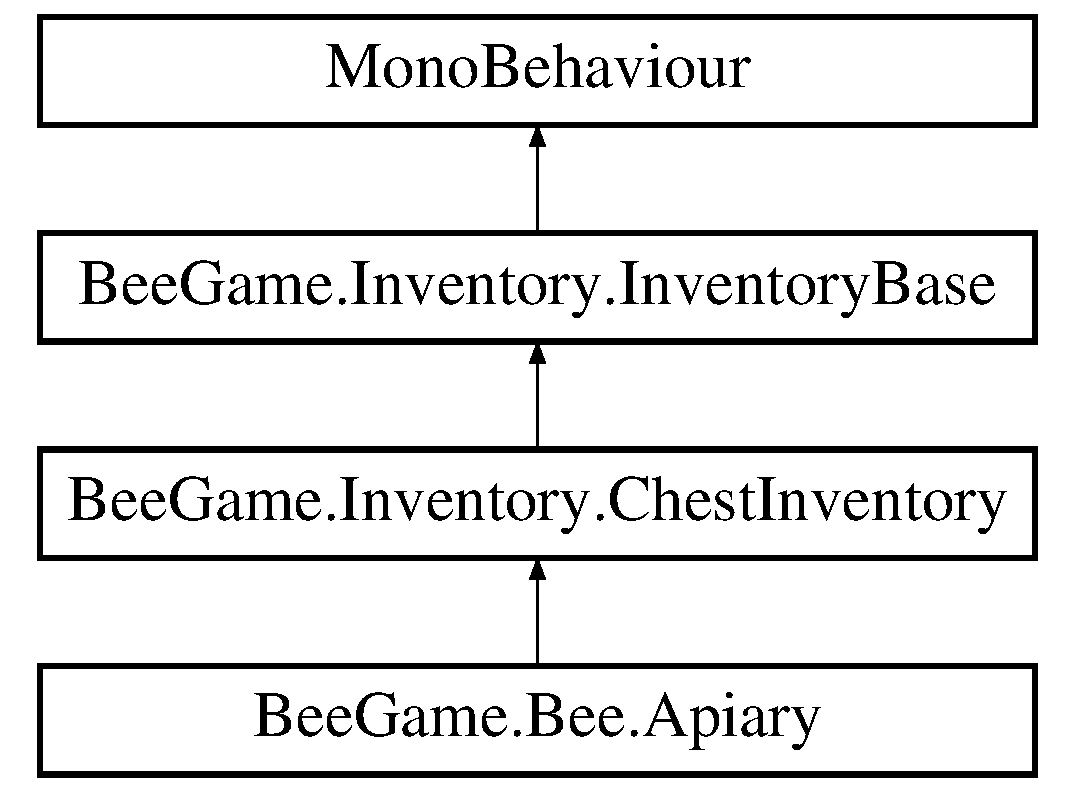
\includegraphics[height=4.000000cm]{class_bee_game_1_1_bee_1_1_apiary}
\end{center}
\end{figure}
\subsection*{Public Attributes}
\begin{DoxyCompactItemize}
\item 
Slider \hyperlink{class_bee_game_1_1_bee_1_1_apiary_a7af4d39f709090d5e5f0c8877e3bbb8d}{ticker}
\item 
\hyperlink{struct_bee_game_1_1_bee_1_1_bee_data}{Bee\+Data} \hyperlink{class_bee_game_1_1_bee_1_1_apiary_a3b3bbe1a8ba0be1c3310a2660b1cdf42}{combining\+Bee}
\item 
\hyperlink{struct_bee_game_1_1_bee_1_1_bee_data}{Bee\+Data} \mbox{[}$\,$\mbox{]} \hyperlink{class_bee_game_1_1_bee_1_1_apiary_abcab0d8cecc18c58a9d01cdf997c7420}{bees}
\item 
\hyperlink{struct_bee_game_1_1_bee_1_1_bee_data}{Bee\+Data} \mbox{[}$\,$\mbox{]} \hyperlink{class_bee_game_1_1_bee_1_1_apiary_a930b4325062b0d6c80581784c23976e8}{new\+Bees}
\end{DoxyCompactItemize}
\subsection*{Private Member Functions}
\begin{DoxyCompactItemize}
\item 
void \hyperlink{class_bee_game_1_1_bee_1_1_apiary_abdaff537d5798876ccbcb8dff82df4d7}{Update} ()
\item 
void \hyperlink{class_bee_game_1_1_bee_1_1_apiary_a13ae008ce398b022806823585c6eb6de}{Reduce\+Timer} ()
\item 
bool \hyperlink{class_bee_game_1_1_bee_1_1_apiary_ac8dbe3e7896909c1fd16f4f998f7b137}{Check\+For\+Bees} ()
\item 
void \hyperlink{class_bee_game_1_1_bee_1_1_apiary_a5e302eef156ac1610cb37720d41b8077}{Combine\+Bees} (\hyperlink{namespace_bee_game_1_1_enums_a9376a1582db99d20c756e24de728944f}{Bee\+Type} type)
\item 
void \hyperlink{class_bee_game_1_1_bee_1_1_apiary_aaa6f9e38434722e3db40ae753a8bb752}{Make\+Items} (\hyperlink{struct_bee_game_1_1_items_1_1_item}{Item}\mbox{[}$\,$\mbox{]} \+\_\+items)
\item 
\hyperlink{struct_bee_game_1_1_items_1_1_item}{Item} \mbox{[}$\,$\mbox{]} \hyperlink{class_bee_game_1_1_bee_1_1_apiary_abb65875e61a806c8b2787d0c7d8229bd}{Return\+Items} (\hyperlink{struct_bee_game_1_1_bee_1_1_bee_data}{Bee\+Data}\mbox{[}$\,$\mbox{]} \+\_\+bees)
\item 
bool \hyperlink{class_bee_game_1_1_bee_1_1_apiary_aa142a57151e9d0ea82e06b22ee530137}{Check\+Slots\+Empty} ()
\begin{DoxyCompactList}\small\item\em Checks if the slots that the new items will be put into are empty \end{DoxyCompactList}\item 
\hyperlink{struct_bee_game_1_1_bee_1_1_bee_data}{Bee\+Data} \mbox{[}$\,$\mbox{]} \hyperlink{class_bee_game_1_1_bee_1_1_apiary_a4aca0b267cdb220e7377165e30eb0324}{Get\+Bees} ()
\begin{DoxyCompactList}\small\item\em Gets the \hyperlink{namespace_bee_game_1_1_items}{Items} in \hyperlink{class_bee_game_1_1_inventory_1_1_inventory_base_a48dcba7ad7bfa1bed8c9ae290fb32857}{inventory\+G\+UI} positons 25 -\/ 26 \end{DoxyCompactList}\item 
\hyperlink{struct_bee_game_1_1_bee_1_1_bee_data}{Bee\+Data} \hyperlink{class_bee_game_1_1_bee_1_1_apiary_ae3a597a3e45de14511f10d17bd5d539b}{New\+Bee} (\hyperlink{struct_bee_game_1_1_bee_1_1_bee_data}{Bee\+Data}\mbox{[}$\,$\mbox{]} \+\_\+bees)
\begin{DoxyCompactList}\small\item\em Makes a New \hyperlink{namespace_bee_game_1_1_bee}{Bee} missing the bee type \end{DoxyCompactList}\item 
\hyperlink{namespace_bee_game_1_1_enums_aa2ead984825678d83c42d48f6382619c}{Bee\+Species} \hyperlink{class_bee_game_1_1_bee_1_1_apiary_ae8d3e50eae58fd390e27203d76124f27}{Return\+Bee\+Species} (\hyperlink{struct_bee_game_1_1_bee_1_1_bee_data}{Bee\+Data} bee)
\begin{DoxyCompactList}\small\item\em Returns the new bee species that the bees allel is based on the combination weights see\+: Bee\+Dictionarys.\+bee\+Mutation\+Chance \end{DoxyCompactList}\item 
float \hyperlink{class_bee_game_1_1_bee_1_1_apiary_a1523391d65f498bd64df18f62840c2f0}{Rand} (float\mbox{[}$\,$\mbox{]} weights)
\begin{DoxyCompactList}\small\item\em Will generate a random number between 0 and the total for the given weights \end{DoxyCompactList}\item 
float \mbox{[}$\,$\mbox{]} \hyperlink{class_bee_game_1_1_bee_1_1_apiary_a0baa1876277fd0e541f0f6b2d347e69b}{Get\+Weights} (\hyperlink{namespace_bee_game_1_1_enums_aa2ead984825678d83c42d48f6382619c}{Bee\+Species}\mbox{[}$\,$\mbox{]} types)
\begin{DoxyCompactList}\small\item\em Gets the weights for the given bee species \end{DoxyCompactList}\item 
int \hyperlink{class_bee_game_1_1_bee_1_1_apiary_a2bdcdda97b0d7f0e4717aa2da979ee65}{Return\+Change} (int bee1, int bee2, int max\+Change, int min\+Change=0)
\begin{DoxyCompactList}\small\item\em Returns the ammout of change compared to the old bee the new bees stats will be \end{DoxyCompactList}\item 
int \mbox{[}$\,$\mbox{]} \hyperlink{class_bee_game_1_1_bee_1_1_apiary_a09fe0446372a57b69863b432e0fdee5e}{Temp\+Tol} (\hyperlink{struct_bee_game_1_1_bee_1_1_bee_data}{Bee\+Data} bee)
\item 
int \mbox{[}$\,$\mbox{]} \hyperlink{class_bee_game_1_1_bee_1_1_apiary_a066f8a76bdd01acbaed48e25768f36e4}{Humidity\+Tol} (\hyperlink{struct_bee_game_1_1_bee_1_1_bee_data}{Bee\+Data} bee)
\item 
bool \hyperlink{class_bee_game_1_1_bee_1_1_apiary_a88c438661490f5f8c0213353be1d5cac}{Return\+Nocturnal} (\hyperlink{struct_bee_game_1_1_bee_1_1_bee_data}{Bee\+Data} bee)
\begin{DoxyCompactList}\small\item\em Is the bee nocturnal. Both bees must not have \hyperlink{struct_bee_game_1_1_bee_1_1_bee_data_a4cd90eee8d255726d982116f14b444b2}{Bee\+Data.\+nocturnal} is not null \end{DoxyCompactList}\item 
bool \hyperlink{class_bee_game_1_1_bee_1_1_apiary_a3c794be5d19c1445f3a48ebc82d49980}{Return\+Flyer} (\hyperlink{struct_bee_game_1_1_bee_1_1_bee_data}{Bee\+Data} bee)
\begin{DoxyCompactList}\small\item\em Is the bee a flyer. Both bees must not have \hyperlink{struct_bee_game_1_1_bee_1_1_bee_data_af78a352321613693c3e94c98f655ac63}{Bee\+Data.\+flyer} is not null \end{DoxyCompactList}\end{DoxyCompactItemize}
\subsection*{Private Attributes}
\begin{DoxyCompactItemize}
\item 
bool \hyperlink{class_bee_game_1_1_bee_1_1_apiary_ae6f4b8692da57eba10d3b593430b2384}{is\+Combining}
\item 
System.\+Random \hyperlink{class_bee_game_1_1_bee_1_1_apiary_a272ac8b385ad3a7cd358b0959d561be7}{rand}
\item 
int \hyperlink{class_bee_game_1_1_bee_1_1_apiary_a0bdb20aaaa311091ddc2f4505dfdb17d}{mutation\+Multiplyer} = 1
\end{DoxyCompactItemize}
\subsection*{Additional Inherited Members}


\subsection{Detailed Description}


\begin{DoxyRefDesc}{Todo}
\item[\hyperlink{todo__todo000001}{Todo}]Add summarys to this \end{DoxyRefDesc}


Definition at line 14 of file Apiary.\+cs.



\subsection{Member Function Documentation}
\mbox{\Hypertarget{class_bee_game_1_1_bee_1_1_apiary_ac8dbe3e7896909c1fd16f4f998f7b137}\label{class_bee_game_1_1_bee_1_1_apiary_ac8dbe3e7896909c1fd16f4f998f7b137}} 
\index{Bee\+Game\+::\+Bee\+::\+Apiary@{Bee\+Game\+::\+Bee\+::\+Apiary}!Check\+For\+Bees@{Check\+For\+Bees}}
\index{Check\+For\+Bees@{Check\+For\+Bees}!Bee\+Game\+::\+Bee\+::\+Apiary@{Bee\+Game\+::\+Bee\+::\+Apiary}}
\subsubsection{\texorpdfstring{Check\+For\+Bees()}{CheckForBees()}}
{\footnotesize\ttfamily bool Bee\+Game.\+Bee.\+Apiary.\+Check\+For\+Bees (\begin{DoxyParamCaption}{ }\end{DoxyParamCaption})\hspace{0.3cm}{\ttfamily [private]}}



Definition at line 56 of file Apiary.\+cs.


\begin{DoxyCode}
57         \{
58             \hyperlink{class_bee_game_1_1_bee_1_1_apiary_abcab0d8cecc18c58a9d01cdf997c7420}{bees} = \hyperlink{class_bee_game_1_1_bee_1_1_apiary_a4aca0b267cdb220e7377165e30eb0324}{GetBees}();
59 
60             \textcolor{keywordflow}{if} (\hyperlink{class_bee_game_1_1_bee_1_1_apiary_aa142a57151e9d0ea82e06b22ee530137}{CheckSlotsEmpty}())
61             \{
62                 \textcolor{keywordflow}{if} (\hyperlink{class_bee_game_1_1_bee_1_1_apiary_abcab0d8cecc18c58a9d01cdf997c7420}{bees} != null)
63                 \{
64                     \textcolor{keywordflow}{if}(\hyperlink{class_bee_game_1_1_bee_1_1_apiary_abcab0d8cecc18c58a9d01cdf997c7420}{bees}[0].beeType == \hyperlink{namespace_bee_game_1_1_enums_a9376a1582db99d20c756e24de728944f}{BeeType}.QUEEN)
65                     \{
66                         \hyperlink{class_bee_game_1_1_bee_1_1_apiary_a5e302eef156ac1610cb37720d41b8077}{CombineBees}(\hyperlink{namespace_bee_game_1_1_enums_a9376a1582db99d20c756e24de728944f}{BeeType}.QUEEN);
67                         \textcolor{keywordflow}{return} \textcolor{keyword}{true};
68                     \}
69                     \textcolor{keywordflow}{else} \textcolor{keywordflow}{if} (\hyperlink{class_bee_game_1_1_bee_1_1_apiary_abcab0d8cecc18c58a9d01cdf997c7420}{bees}[0].beeType == \hyperlink{namespace_bee_game_1_1_enums_a9376a1582db99d20c756e24de728944f}{BeeType}.PRINCESS && 
      \hyperlink{class_bee_game_1_1_bee_1_1_apiary_abcab0d8cecc18c58a9d01cdf997c7420}{bees}[1].\hyperlink{struct_bee_game_1_1_bee_1_1_bee_data_acfb6e209ae7bd1b52928580fcce4c743}{beeType} == \hyperlink{namespace_bee_game_1_1_enums_a9376a1582db99d20c756e24de728944f}{BeeType}.DRONE)
70                     \{
71                         \hyperlink{class_bee_game_1_1_bee_1_1_apiary_a5e302eef156ac1610cb37720d41b8077}{CombineBees}(\hyperlink{namespace_bee_game_1_1_enums_a9376a1582db99d20c756e24de728944f}{BeeType}.PRINCESS);
72                         \textcolor{keywordflow}{return} \textcolor{keyword}{true};
73                     \}
74                 \}
75             \}
76 
77             \textcolor{keywordflow}{return} \textcolor{keyword}{false};
78         \}
\end{DoxyCode}
\mbox{\Hypertarget{class_bee_game_1_1_bee_1_1_apiary_aa142a57151e9d0ea82e06b22ee530137}\label{class_bee_game_1_1_bee_1_1_apiary_aa142a57151e9d0ea82e06b22ee530137}} 
\index{Bee\+Game\+::\+Bee\+::\+Apiary@{Bee\+Game\+::\+Bee\+::\+Apiary}!Check\+Slots\+Empty@{Check\+Slots\+Empty}}
\index{Check\+Slots\+Empty@{Check\+Slots\+Empty}!Bee\+Game\+::\+Bee\+::\+Apiary@{Bee\+Game\+::\+Bee\+::\+Apiary}}
\subsubsection{\texorpdfstring{Check\+Slots\+Empty()}{CheckSlotsEmpty()}}
{\footnotesize\ttfamily bool Bee\+Game.\+Bee.\+Apiary.\+Check\+Slots\+Empty (\begin{DoxyParamCaption}{ }\end{DoxyParamCaption})\hspace{0.3cm}{\ttfamily [private]}}



Checks if the slots that the new items will be put into are empty 

\begin{DoxyReturn}{Returns}
true if the slots are empty
\end{DoxyReturn}


Definition at line 157 of file Apiary.\+cs.


\begin{DoxyCode}
158         \{
159             \textcolor{keywordflow}{for} (\textcolor{keywordtype}{int} i = \hyperlink{class_bee_game_1_1_inventory_1_1_inventory_base_a48dcba7ad7bfa1bed8c9ae290fb32857}{inventoryGUI}.Length - 1; i >= 27; i--)
160             \{
161                 \textcolor{keywordflow}{if}(\hyperlink{class_bee_game_1_1_inventory_1_1_inventory_base_a48dcba7ad7bfa1bed8c9ae290fb32857}{inventoryGUI}[i].item.itemId != null)
162                 \{
163                     \textcolor{keywordflow}{return} \textcolor{keyword}{false};
164                 \}
165             \}
166 
167             \textcolor{keywordflow}{return} \textcolor{keyword}{true};
168         \}
\end{DoxyCode}
\mbox{\Hypertarget{class_bee_game_1_1_bee_1_1_apiary_a5e302eef156ac1610cb37720d41b8077}\label{class_bee_game_1_1_bee_1_1_apiary_a5e302eef156ac1610cb37720d41b8077}} 
\index{Bee\+Game\+::\+Bee\+::\+Apiary@{Bee\+Game\+::\+Bee\+::\+Apiary}!Combine\+Bees@{Combine\+Bees}}
\index{Combine\+Bees@{Combine\+Bees}!Bee\+Game\+::\+Bee\+::\+Apiary@{Bee\+Game\+::\+Bee\+::\+Apiary}}
\subsubsection{\texorpdfstring{Combine\+Bees()}{CombineBees()}}
{\footnotesize\ttfamily void Bee\+Game.\+Bee.\+Apiary.\+Combine\+Bees (\begin{DoxyParamCaption}\item[{\hyperlink{namespace_bee_game_1_1_enums_a9376a1582db99d20c756e24de728944f}{Bee\+Type}}]{type }\end{DoxyParamCaption})\hspace{0.3cm}{\ttfamily [private]}}



Definition at line 80 of file Apiary.\+cs.


\begin{DoxyCode}
81         \{
82             \hyperlink{class_bee_game_1_1_bee_1_1_apiary_a272ac8b385ad3a7cd358b0959d561be7}{rand} = \textcolor{keyword}{new} \hyperlink{namespace_system}{System}.Random();
83 
84             \textcolor{keywordflow}{switch} (type)
85             \{
86                 \textcolor{keywordflow}{case} \hyperlink{namespace_bee_game_1_1_enums_a9376a1582db99d20c756e24de728944f}{BeeType}.QUEEN:
87                     \hyperlink{class_bee_game_1_1_bee_1_1_apiary_a3b3bbe1a8ba0be1c3310a2660b1cdf42}{combiningBee} = \hyperlink{class_bee_game_1_1_bee_1_1_apiary_abcab0d8cecc18c58a9d01cdf997c7420}{bees}[0];
88                     \textcolor{keywordflow}{break};
89                 \textcolor{keywordflow}{case} \hyperlink{namespace_bee_game_1_1_enums_a9376a1582db99d20c756e24de728944f}{BeeType}.PRINCESS:
90                     \hyperlink{class_bee_game_1_1_bee_1_1_apiary_a3b3bbe1a8ba0be1c3310a2660b1cdf42}{combiningBee} = \hyperlink{class_bee_game_1_1_bee_1_1_apiary_abcab0d8cecc18c58a9d01cdf997c7420}{bees}[0];
91                     \hyperlink{class_bee_game_1_1_bee_1_1_apiary_a3b3bbe1a8ba0be1c3310a2660b1cdf42}{combiningBee}.\hyperlink{struct_bee_game_1_1_bee_1_1_bee_data_ab12331d23b41365d0a1be0d7eba7fa0f}{combiningData}.
      \hyperlink{struct_bee_game_1_1_bee_1_1_combining_bee_data_abdf4646728337da76097aed9b74347ae}{ToCombiningBeeData}(\hyperlink{class_bee_game_1_1_bee_1_1_apiary_abcab0d8cecc18c58a9d01cdf997c7420}{bees}[1]);
92                     \hyperlink{class_bee_game_1_1_inventory_1_1_inventory_base_a48dcba7ad7bfa1bed8c9ae290fb32857}{inventoryGUI}[25].\hyperlink{class_bee_game_1_1_inventory_1_1_inventory_slot_a31b201e7eef9ed0001a447b3f76a7a81}{item}.\hyperlink{struct_bee_game_1_1_items_1_1_item_a0593f3b7b3ff5daa864f3c6d0ccd77ca}{beeItem} = 
      \hyperlink{class_bee_game_1_1_bee_1_1_apiary_a3b3bbe1a8ba0be1c3310a2660b1cdf42}{combiningBee};
93                     \hyperlink{class_bee_game_1_1_inventory_1_1_inventory_base_a48dcba7ad7bfa1bed8c9ae290fb32857}{inventoryGUI}[25].\hyperlink{class_bee_game_1_1_inventory_1_1_inventory_slot_a31b201e7eef9ed0001a447b3f76a7a81}{item}.\hyperlink{struct_bee_game_1_1_items_1_1_item_a80c66aa30f64c498640a4b0ba1ec37b0}{SetBeeType}(
      \hyperlink{namespace_bee_game_1_1_enums_a9376a1582db99d20c756e24de728944f}{BeeType}.QUEEN);
94                     \hyperlink{class_bee_game_1_1_inventory_1_1_inventory_base_a48dcba7ad7bfa1bed8c9ae290fb32857}{inventoryGUI}[26].\hyperlink{class_bee_game_1_1_inventory_1_1_inventory_slot_a31b201e7eef9ed0001a447b3f76a7a81}{item} = \textcolor{keyword}{new} \hyperlink{struct_bee_game_1_1_items_1_1_item}{Item}();
95                     \textcolor{keywordflow}{break};
96                 \textcolor{keywordflow}{default}:
97                     \textcolor{keywordflow}{break};
98             \}
99             
100             \hyperlink{class_bee_game_1_1_bee_1_1_apiary_a930b4325062b0d6c80581784c23976e8}{newBees} = \textcolor{keyword}{new} BeeData[\hyperlink{class_bee_game_1_1_bee_1_1_apiary_a3b3bbe1a8ba0be1c3310a2660b1cdf42}{combiningBee}.\hyperlink{struct_bee_game_1_1_bee_1_1_bee_data_a12b5a0d54c6c9162a69a88c349b044d1}{pFertility}];
101 
102             \textcolor{keywordflow}{for} (\textcolor{keywordtype}{int} i = 0; i < \hyperlink{class_bee_game_1_1_bee_1_1_apiary_a930b4325062b0d6c80581784c23976e8}{newBees}.Length; i++)
103             \{
104                 \hyperlink{class_bee_game_1_1_bee_1_1_apiary_a930b4325062b0d6c80581784c23976e8}{newBees}[i] = \hyperlink{class_bee_game_1_1_bee_1_1_apiary_ae3a597a3e45de14511f10d17bd5d539b}{NewBee}(\hyperlink{class_bee_game_1_1_bee_1_1_apiary_abcab0d8cecc18c58a9d01cdf997c7420}{bees});
105             \}
106 
107             \hyperlink{class_bee_game_1_1_bee_1_1_apiary_a7af4d39f709090d5e5f0c8877e3bbb8d}{ticker}.maxValue = (float)\hyperlink{class_bee_game_1_1_bee_1_1_apiary_abcab0d8cecc18c58a9d01cdf997c7420}{bees}[0].pLifespan;
108             \hyperlink{class_bee_game_1_1_bee_1_1_apiary_a7af4d39f709090d5e5f0c8877e3bbb8d}{ticker}.value = \hyperlink{class_bee_game_1_1_bee_1_1_apiary_a7af4d39f709090d5e5f0c8877e3bbb8d}{ticker}.maxValue;
109         \}
\end{DoxyCode}
\mbox{\Hypertarget{class_bee_game_1_1_bee_1_1_apiary_a4aca0b267cdb220e7377165e30eb0324}\label{class_bee_game_1_1_bee_1_1_apiary_a4aca0b267cdb220e7377165e30eb0324}} 
\index{Bee\+Game\+::\+Bee\+::\+Apiary@{Bee\+Game\+::\+Bee\+::\+Apiary}!Get\+Bees@{Get\+Bees}}
\index{Get\+Bees@{Get\+Bees}!Bee\+Game\+::\+Bee\+::\+Apiary@{Bee\+Game\+::\+Bee\+::\+Apiary}}
\subsubsection{\texorpdfstring{Get\+Bees()}{GetBees()}}
{\footnotesize\ttfamily \hyperlink{struct_bee_game_1_1_bee_1_1_bee_data}{Bee\+Data} \mbox{[}$\,$\mbox{]} Bee\+Game.\+Bee.\+Apiary.\+Get\+Bees (\begin{DoxyParamCaption}{ }\end{DoxyParamCaption})\hspace{0.3cm}{\ttfamily [private]}}



Gets the \hyperlink{namespace_bee_game_1_1_items}{Items} in \hyperlink{class_bee_game_1_1_inventory_1_1_inventory_base_a48dcba7ad7bfa1bed8c9ae290fb32857}{inventory\+G\+UI} positons 25 -\/ 26 

\begin{DoxyReturn}{Returns}
Bee\+Data\mbox{[}$\,$\mbox{]} of the bees in \hyperlink{class_bee_game_1_1_inventory_1_1_inventory_base_a48dcba7ad7bfa1bed8c9ae290fb32857}{inventory\+G\+UI} positons 25 -\/ 26
\end{DoxyReturn}


Definition at line 174 of file Apiary.\+cs.


\begin{DoxyCode}
175         \{
176             BeeData bee1 = \textcolor{keyword}{new} BeeData();
177             BeeData bee2 = \textcolor{keyword}{new} BeeData();
178 
179             \textcolor{keywordtype}{bool} returnNull = \textcolor{keyword}{true};
180 
181             \textcolor{keywordflow}{if} (\hyperlink{class_bee_game_1_1_inventory_1_1_inventory_base_a48dcba7ad7bfa1bed8c9ae290fb32857}{inventoryGUI}[25].item.itemId != null)
182             \{
183                 \textcolor{keywordflow}{if} (\hyperlink{class_bee_game_1_1_inventory_1_1_inventory_base_a48dcba7ad7bfa1bed8c9ae290fb32857}{inventoryGUI}[25].item.itemType == \hyperlink{namespace_bee_game_1_1_enums_aa1fa1a04627915b8e72d3bb1c5c3fa82}{ItemType}.BEE)
184                 \{
185                     bee1 = \hyperlink{class_bee_game_1_1_inventory_1_1_inventory_base_a48dcba7ad7bfa1bed8c9ae290fb32857}{inventoryGUI}[25].\hyperlink{class_bee_game_1_1_inventory_1_1_inventory_slot_a31b201e7eef9ed0001a447b3f76a7a81}{item}.\hyperlink{struct_bee_game_1_1_items_1_1_item_a3751a7c44aa4ff5975f1487ade757d9f}{ReturnBeeData}();
186                     returnNull = \textcolor{keyword}{false};
187                 \}
188             \}
189             \textcolor{keywordflow}{if} (\hyperlink{class_bee_game_1_1_inventory_1_1_inventory_base_a48dcba7ad7bfa1bed8c9ae290fb32857}{inventoryGUI}[26].item.itemId != null)
190             \{
191                 \textcolor{keywordflow}{if} (\hyperlink{class_bee_game_1_1_inventory_1_1_inventory_base_a48dcba7ad7bfa1bed8c9ae290fb32857}{inventoryGUI}[26].item.itemType == \hyperlink{namespace_bee_game_1_1_enums_aa1fa1a04627915b8e72d3bb1c5c3fa82}{ItemType}.BEE)
192                 \{
193                     bee2 = \hyperlink{class_bee_game_1_1_inventory_1_1_inventory_base_a48dcba7ad7bfa1bed8c9ae290fb32857}{inventoryGUI}[26].\hyperlink{class_bee_game_1_1_inventory_1_1_inventory_slot_a31b201e7eef9ed0001a447b3f76a7a81}{item}.\hyperlink{struct_bee_game_1_1_items_1_1_item_a3751a7c44aa4ff5975f1487ade757d9f}{ReturnBeeData}();
194                 \}
195             \}
196 
197             \textcolor{keywordflow}{if}(!returnNull)
198             \{
199                 \textcolor{keywordflow}{return} \textcolor{keyword}{new} BeeData[2] \{ bee1, bee2 \};
200             \}
201             \textcolor{keywordflow}{else}
202             \{
203                 \textcolor{keywordflow}{return} null;
204             \}
205         \}
\end{DoxyCode}
\mbox{\Hypertarget{class_bee_game_1_1_bee_1_1_apiary_a0baa1876277fd0e541f0f6b2d347e69b}\label{class_bee_game_1_1_bee_1_1_apiary_a0baa1876277fd0e541f0f6b2d347e69b}} 
\index{Bee\+Game\+::\+Bee\+::\+Apiary@{Bee\+Game\+::\+Bee\+::\+Apiary}!Get\+Weights@{Get\+Weights}}
\index{Get\+Weights@{Get\+Weights}!Bee\+Game\+::\+Bee\+::\+Apiary@{Bee\+Game\+::\+Bee\+::\+Apiary}}
\subsubsection{\texorpdfstring{Get\+Weights()}{GetWeights()}}
{\footnotesize\ttfamily float \mbox{[}$\,$\mbox{]} Bee\+Game.\+Bee.\+Apiary.\+Get\+Weights (\begin{DoxyParamCaption}\item[{\hyperlink{namespace_bee_game_1_1_enums_aa2ead984825678d83c42d48f6382619c}{Bee\+Species} \mbox{[}$\,$\mbox{]}}]{types }\end{DoxyParamCaption})\hspace{0.3cm}{\ttfamily [private]}}



Gets the weights for the given bee species 


\begin{DoxyParams}{Parameters}
{\em types} & Bee\+Species\mbox{[}$\,$\mbox{]}\\
\hline
\end{DoxyParams}
\begin{DoxyReturn}{Returns}
\hyperlink{}{for the } weights
\end{DoxyReturn}


Definition at line 319 of file Apiary.\+cs.


\begin{DoxyCode}
320         \{
321             \textcolor{keywordtype}{float}[] weights = \textcolor{keyword}{new} \textcolor{keywordtype}{float}[types.Length + 2];
322             var totalWeight = 0f;
323 
324             \textcolor{keywordflow}{for} (\textcolor{keywordtype}{int} i = 0; i < types.Length; i++)
325             \{
326                 var weight = \hyperlink{class_bee_game_1_1_core_1_1_bee_dictionarys}{BeeDictionarys}.\hyperlink{class_bee_game_1_1_core_1_1_bee_dictionarys_adb5fe5760a94dbff606bc1d20ee67aaa}{GetMutationChance}(types[i]);
327                 weights[i] = weight;
328                 totalWeight += weight;
329             \}
330 
331             var half = (1f - totalWeight) / 2;
332 
333             weights[weights.Length - 2] = half;
334             weights[weights.Length - 1] = half;
335 
336             \textcolor{keywordflow}{return} weights;
337         \}
\end{DoxyCode}
\mbox{\Hypertarget{class_bee_game_1_1_bee_1_1_apiary_a066f8a76bdd01acbaed48e25768f36e4}\label{class_bee_game_1_1_bee_1_1_apiary_a066f8a76bdd01acbaed48e25768f36e4}} 
\index{Bee\+Game\+::\+Bee\+::\+Apiary@{Bee\+Game\+::\+Bee\+::\+Apiary}!Humidity\+Tol@{Humidity\+Tol}}
\index{Humidity\+Tol@{Humidity\+Tol}!Bee\+Game\+::\+Bee\+::\+Apiary@{Bee\+Game\+::\+Bee\+::\+Apiary}}
\subsubsection{\texorpdfstring{Humidity\+Tol()}{HumidityTol()}}
{\footnotesize\ttfamily int \mbox{[}$\,$\mbox{]} Bee\+Game.\+Bee.\+Apiary.\+Humidity\+Tol (\begin{DoxyParamCaption}\item[{\hyperlink{struct_bee_game_1_1_bee_1_1_bee_data}{Bee\+Data}}]{bee }\end{DoxyParamCaption})\hspace{0.3cm}{\ttfamily [private]}}



Definition at line 377 of file Apiary.\+cs.


\begin{DoxyCode}
378         \{
379             BeeData[] \_bees = \textcolor{keyword}{new} BeeData[2] \{ bee, bee.combiningData.ToBeeData() \};
380             \textcolor{keywordflow}{return} \_bees[\hyperlink{class_bee_game_1_1_bee_1_1_apiary_a272ac8b385ad3a7cd358b0959d561be7}{rand}.Next(0, 2)].humidTol;
381         \}
\end{DoxyCode}
\mbox{\Hypertarget{class_bee_game_1_1_bee_1_1_apiary_aaa6f9e38434722e3db40ae753a8bb752}\label{class_bee_game_1_1_bee_1_1_apiary_aaa6f9e38434722e3db40ae753a8bb752}} 
\index{Bee\+Game\+::\+Bee\+::\+Apiary@{Bee\+Game\+::\+Bee\+::\+Apiary}!Make\+Items@{Make\+Items}}
\index{Make\+Items@{Make\+Items}!Bee\+Game\+::\+Bee\+::\+Apiary@{Bee\+Game\+::\+Bee\+::\+Apiary}}
\subsubsection{\texorpdfstring{Make\+Items()}{MakeItems()}}
{\footnotesize\ttfamily void Bee\+Game.\+Bee.\+Apiary.\+Make\+Items (\begin{DoxyParamCaption}\item[{\hyperlink{struct_bee_game_1_1_items_1_1_item}{Item} \mbox{[}$\,$\mbox{]}}]{\+\_\+items }\end{DoxyParamCaption})\hspace{0.3cm}{\ttfamily [private]}}



Definition at line 111 of file Apiary.\+cs.


\begin{DoxyCode}
112         \{
113             \textcolor{keywordflow}{if} (\_items != null)
114             \{
115                 \textcolor{keywordflow}{for} (\textcolor{keywordtype}{int} i = 0; i < \_items.Length; i++)
116                 \{
117                     \textcolor{keywordflow}{for} (\textcolor{keywordtype}{int} h = \hyperlink{class_bee_game_1_1_inventory_1_1_inventory_base_a48dcba7ad7bfa1bed8c9ae290fb32857}{inventoryGUI}.Length - 1; h >= 27; h--)
118                     \{
119                         \textcolor{keywordflow}{if} (\hyperlink{class_bee_game_1_1_inventory_1_1_inventory_base_a48dcba7ad7bfa1bed8c9ae290fb32857}{inventoryGUI}[h].item.itemId == null)
120                         \{
121                             \hyperlink{class_bee_game_1_1_inventory_1_1_inventory_base_a48dcba7ad7bfa1bed8c9ae290fb32857}{inventoryGUI}[h].\hyperlink{class_bee_game_1_1_inventory_1_1_inventory_slot_a31b201e7eef9ed0001a447b3f76a7a81}{item} = \_items[i];
122                             \textcolor{keywordflow}{break};
123                         \}
124                     \}
125                 \}
126             \}
127 
128             \hyperlink{class_bee_game_1_1_inventory_1_1_inventory_base_a48dcba7ad7bfa1bed8c9ae290fb32857}{inventoryGUI}[25].\hyperlink{class_bee_game_1_1_inventory_1_1_inventory_slot_a31b201e7eef9ed0001a447b3f76a7a81}{item} = \textcolor{keyword}{new} \hyperlink{struct_bee_game_1_1_items_1_1_item}{Item}();
129         \}
\end{DoxyCode}
\mbox{\Hypertarget{class_bee_game_1_1_bee_1_1_apiary_ae3a597a3e45de14511f10d17bd5d539b}\label{class_bee_game_1_1_bee_1_1_apiary_ae3a597a3e45de14511f10d17bd5d539b}} 
\index{Bee\+Game\+::\+Bee\+::\+Apiary@{Bee\+Game\+::\+Bee\+::\+Apiary}!New\+Bee@{New\+Bee}}
\index{New\+Bee@{New\+Bee}!Bee\+Game\+::\+Bee\+::\+Apiary@{Bee\+Game\+::\+Bee\+::\+Apiary}}
\subsubsection{\texorpdfstring{New\+Bee()}{NewBee()}}
{\footnotesize\ttfamily \hyperlink{struct_bee_game_1_1_bee_1_1_bee_data}{Bee\+Data} Bee\+Game.\+Bee.\+Apiary.\+New\+Bee (\begin{DoxyParamCaption}\item[{\hyperlink{struct_bee_game_1_1_bee_1_1_bee_data}{Bee\+Data} \mbox{[}$\,$\mbox{]}}]{\+\_\+bees }\end{DoxyParamCaption})\hspace{0.3cm}{\ttfamily [private]}}



Makes a New \hyperlink{namespace_bee_game_1_1_bee}{Bee} missing the bee type 


\begin{DoxyParams}{Parameters}
{\em \+\_\+bees} & \hyperlink{struct_bee_game_1_1_bee_1_1_bee_data}{Bee\+Data} without a \hyperlink{struct_bee_game_1_1_bee_1_1_bee_data_acfb6e209ae7bd1b52928580fcce4c743}{Bee\+Data.\+bee\+Type}\\
\hline
\end{DoxyParams}
Setting the primary stats of the bee (Phenotype) /summary$>$

Setting the secondary trait of the bee (Secondary) /summary$>$

Sets the temp\+Pref and temp\+Tol of the new bee /summary$>$

Sets the humid\+Pref and humid\+Tol of the new bee /summary$>$ 

Definition at line 211 of file Apiary.\+cs.


\begin{DoxyCode}
212         \{
213             BeeData newBee = \textcolor{keyword}{new} BeeData();
214 
218             newBee.pSpecies = \hyperlink{class_bee_game_1_1_bee_1_1_apiary_ae8d3e50eae58fd390e27203d76124f27}{ReturnBeeSpecies}(\hyperlink{class_bee_game_1_1_bee_1_1_apiary_a3b3bbe1a8ba0be1c3310a2660b1cdf42}{combiningBee});
219             newBee.pLifespan = (\hyperlink{namespace_bee_game_1_1_enums_ae3853807ded2f4d99a0d4a7fb4b2bc46}{BeeLifeSpan})\hyperlink{class_bee_game_1_1_bee_1_1_apiary_a2bdcdda97b0d7f0e4717aa2da979ee65}{ReturnChange}((\textcolor{keywordtype}{int})
      \hyperlink{class_bee_game_1_1_bee_1_1_apiary_a3b3bbe1a8ba0be1c3310a2660b1cdf42}{combiningBee}.\hyperlink{struct_bee_game_1_1_bee_1_1_bee_data_af5c384db9813e463bb0d66cb8b443d87}{sLifespan}, (int)\hyperlink{class_bee_game_1_1_bee_1_1_apiary_a3b3bbe1a8ba0be1c3310a2660b1cdf42}{combiningBee}.
      \hyperlink{struct_bee_game_1_1_bee_1_1_bee_data_ab12331d23b41365d0a1be0d7eba7fa0f}{combiningData}.\hyperlink{struct_bee_game_1_1_bee_1_1_combining_bee_data_a2635fae2aa8e50991d7733624883e671}{sLifespan}, (\textcolor{keywordtype}{int})\hyperlink{namespace_bee_game_1_1_enums_ae3853807ded2f4d99a0d4a7fb4b2bc46}{BeeLifeSpan}.SEATURTLE);
220             newBee.pFertility = (uint)\hyperlink{class_bee_game_1_1_bee_1_1_apiary_a2bdcdda97b0d7f0e4717aa2da979ee65}{ReturnChange}((\textcolor{keywordtype}{int})\hyperlink{class_bee_game_1_1_bee_1_1_apiary_a3b3bbe1a8ba0be1c3310a2660b1cdf42}{combiningBee}.
      \hyperlink{struct_bee_game_1_1_bee_1_1_bee_data_a20a4084334bbbba3942f67622596b596}{sFertility}, (int)\hyperlink{class_bee_game_1_1_bee_1_1_apiary_a3b3bbe1a8ba0be1c3310a2660b1cdf42}{combiningBee}.\hyperlink{struct_bee_game_1_1_bee_1_1_bee_data_ab12331d23b41365d0a1be0d7eba7fa0f}{combiningData}.
      \hyperlink{struct_bee_game_1_1_bee_1_1_combining_bee_data_a02566c65413bebc23e767561c17510d5}{sFertility}, 5, 2);
221             newBee.pEffect = (\hyperlink{namespace_bee_game_1_1_enums_acf7ae32a86385a40fc0c7b55af95c6c3}{BeeEffect})\hyperlink{class_bee_game_1_1_bee_1_1_apiary_a2bdcdda97b0d7f0e4717aa2da979ee65}{ReturnChange}((\textcolor{keywordtype}{int})
      \hyperlink{class_bee_game_1_1_bee_1_1_apiary_a3b3bbe1a8ba0be1c3310a2660b1cdf42}{combiningBee}.\hyperlink{struct_bee_game_1_1_bee_1_1_bee_data_ac65b550d77e529a62cb60acf86502bc2}{sEffect}, (int)\hyperlink{class_bee_game_1_1_bee_1_1_apiary_a3b3bbe1a8ba0be1c3310a2660b1cdf42}{combiningBee}.
      \hyperlink{struct_bee_game_1_1_bee_1_1_bee_data_ab12331d23b41365d0a1be0d7eba7fa0f}{combiningData}.\hyperlink{struct_bee_game_1_1_bee_1_1_combining_bee_data_a6706a04242c477e5934d779fde7e7b8e}{sEffect}, (\textcolor{keywordtype}{int})\hyperlink{namespace_bee_game_1_1_enums_acf7ae32a86385a40fc0c7b55af95c6c3}{BeeEffect}.POSION);
222             newBee.pProdSpeed = (\hyperlink{namespace_bee_game_1_1_enums_afee18200a21cc4b8e1d0cdb669930f14}{BeeProductionSpeed})
      \hyperlink{class_bee_game_1_1_bee_1_1_apiary_a2bdcdda97b0d7f0e4717aa2da979ee65}{ReturnChange}((\textcolor{keywordtype}{int})\hyperlink{class_bee_game_1_1_bee_1_1_apiary_a3b3bbe1a8ba0be1c3310a2660b1cdf42}{combiningBee}.\hyperlink{struct_bee_game_1_1_bee_1_1_bee_data_af2e94ee206fd06b8314888f8ba3d56e9}{sProdSpeed}, (int)
      \hyperlink{class_bee_game_1_1_bee_1_1_apiary_a3b3bbe1a8ba0be1c3310a2660b1cdf42}{combiningBee}.\hyperlink{struct_bee_game_1_1_bee_1_1_bee_data_ab12331d23b41365d0a1be0d7eba7fa0f}{combiningData}.\hyperlink{struct_bee_game_1_1_bee_1_1_combining_bee_data_a253d2a55fe2cb1a3d01492a6f961b995}{sProdSpeed}, (\textcolor{keywordtype}{int})
      \hyperlink{namespace_bee_game_1_1_enums_afee18200a21cc4b8e1d0cdb669930f14}{BeeProductionSpeed}.FAST);
223 
227             newBee.sSpecies = \hyperlink{class_bee_game_1_1_bee_1_1_apiary_ae8d3e50eae58fd390e27203d76124f27}{ReturnBeeSpecies}(\hyperlink{class_bee_game_1_1_bee_1_1_apiary_a3b3bbe1a8ba0be1c3310a2660b1cdf42}{combiningBee});
228             newBee.sLifespan = (\hyperlink{namespace_bee_game_1_1_enums_ae3853807ded2f4d99a0d4a7fb4b2bc46}{BeeLifeSpan})\hyperlink{class_bee_game_1_1_bee_1_1_apiary_a2bdcdda97b0d7f0e4717aa2da979ee65}{ReturnChange}((\textcolor{keywordtype}{int})
      \hyperlink{class_bee_game_1_1_bee_1_1_apiary_a3b3bbe1a8ba0be1c3310a2660b1cdf42}{combiningBee}.\hyperlink{struct_bee_game_1_1_bee_1_1_bee_data_af5c384db9813e463bb0d66cb8b443d87}{sLifespan}, (int)\hyperlink{class_bee_game_1_1_bee_1_1_apiary_a3b3bbe1a8ba0be1c3310a2660b1cdf42}{combiningBee}.
      \hyperlink{struct_bee_game_1_1_bee_1_1_bee_data_ab12331d23b41365d0a1be0d7eba7fa0f}{combiningData}.\hyperlink{struct_bee_game_1_1_bee_1_1_combining_bee_data_a2635fae2aa8e50991d7733624883e671}{sLifespan}, (\textcolor{keywordtype}{int})\hyperlink{namespace_bee_game_1_1_enums_ae3853807ded2f4d99a0d4a7fb4b2bc46}{BeeLifeSpan}.SEATURTLE);
229             newBee.sFertility = (uint)\hyperlink{class_bee_game_1_1_bee_1_1_apiary_a2bdcdda97b0d7f0e4717aa2da979ee65}{ReturnChange}((\textcolor{keywordtype}{int})\hyperlink{class_bee_game_1_1_bee_1_1_apiary_a3b3bbe1a8ba0be1c3310a2660b1cdf42}{combiningBee}.
      \hyperlink{struct_bee_game_1_1_bee_1_1_bee_data_a20a4084334bbbba3942f67622596b596}{sFertility}, (int)\hyperlink{class_bee_game_1_1_bee_1_1_apiary_a3b3bbe1a8ba0be1c3310a2660b1cdf42}{combiningBee}.\hyperlink{struct_bee_game_1_1_bee_1_1_bee_data_ab12331d23b41365d0a1be0d7eba7fa0f}{combiningData}.
      \hyperlink{struct_bee_game_1_1_bee_1_1_combining_bee_data_a02566c65413bebc23e767561c17510d5}{sFertility}, 5, 2);
230             newBee.sEffect = (\hyperlink{namespace_bee_game_1_1_enums_acf7ae32a86385a40fc0c7b55af95c6c3}{BeeEffect})\hyperlink{class_bee_game_1_1_bee_1_1_apiary_a2bdcdda97b0d7f0e4717aa2da979ee65}{ReturnChange}((\textcolor{keywordtype}{int})
      \hyperlink{class_bee_game_1_1_bee_1_1_apiary_a3b3bbe1a8ba0be1c3310a2660b1cdf42}{combiningBee}.\hyperlink{struct_bee_game_1_1_bee_1_1_bee_data_ac65b550d77e529a62cb60acf86502bc2}{sEffect}, (int)\hyperlink{class_bee_game_1_1_bee_1_1_apiary_a3b3bbe1a8ba0be1c3310a2660b1cdf42}{combiningBee}.
      \hyperlink{struct_bee_game_1_1_bee_1_1_bee_data_ab12331d23b41365d0a1be0d7eba7fa0f}{combiningData}.\hyperlink{struct_bee_game_1_1_bee_1_1_combining_bee_data_a6706a04242c477e5934d779fde7e7b8e}{sEffect}, (\textcolor{keywordtype}{int})\hyperlink{namespace_bee_game_1_1_enums_acf7ae32a86385a40fc0c7b55af95c6c3}{BeeEffect}.POSION);
231             newBee.sProdSpeed = (\hyperlink{namespace_bee_game_1_1_enums_afee18200a21cc4b8e1d0cdb669930f14}{BeeProductionSpeed})
      \hyperlink{class_bee_game_1_1_bee_1_1_apiary_a2bdcdda97b0d7f0e4717aa2da979ee65}{ReturnChange}((\textcolor{keywordtype}{int})\hyperlink{class_bee_game_1_1_bee_1_1_apiary_a3b3bbe1a8ba0be1c3310a2660b1cdf42}{combiningBee}.\hyperlink{struct_bee_game_1_1_bee_1_1_bee_data_af2e94ee206fd06b8314888f8ba3d56e9}{sProdSpeed}, (int)
      \hyperlink{class_bee_game_1_1_bee_1_1_apiary_a3b3bbe1a8ba0be1c3310a2660b1cdf42}{combiningBee}.\hyperlink{struct_bee_game_1_1_bee_1_1_bee_data_ab12331d23b41365d0a1be0d7eba7fa0f}{combiningData}.\hyperlink{struct_bee_game_1_1_bee_1_1_combining_bee_data_a253d2a55fe2cb1a3d01492a6f961b995}{sProdSpeed}, (\textcolor{keywordtype}{int})
      \hyperlink{namespace_bee_game_1_1_enums_afee18200a21cc4b8e1d0cdb669930f14}{BeeProductionSpeed}.FAST);
232 
236             newBee.tempPref = (\hyperlink{namespace_bee_game_1_1_enums_a9db0f9ac859fab168654d657f248b024}{BeeTempPreferance})\hyperlink{class_bee_game_1_1_bee_1_1_apiary_a2bdcdda97b0d7f0e4717aa2da979ee65}{ReturnChange}((\textcolor{keywordtype}{int})
      \hyperlink{class_bee_game_1_1_bee_1_1_apiary_a3b3bbe1a8ba0be1c3310a2660b1cdf42}{combiningBee}.\hyperlink{struct_bee_game_1_1_bee_1_1_bee_data_ab7c3b5184d04319359a7f31fa0a4dc8c}{tempPref}, (int)\hyperlink{class_bee_game_1_1_bee_1_1_apiary_a3b3bbe1a8ba0be1c3310a2660b1cdf42}{combiningBee}.
      \hyperlink{struct_bee_game_1_1_bee_1_1_bee_data_ab12331d23b41365d0a1be0d7eba7fa0f}{combiningData}.\hyperlink{struct_bee_game_1_1_bee_1_1_combining_bee_data_a93f8cb5caf0b68dd597da1b3ab9e27b5}{tempPref}, (\textcolor{keywordtype}{int})\hyperlink{namespace_bee_game_1_1_enums_a9db0f9ac859fab168654d657f248b024}{BeeTempPreferance}.HELL);
237             newBee.tempTol = \hyperlink{class_bee_game_1_1_bee_1_1_apiary_a09fe0446372a57b69863b432e0fdee5e}{TempTol}(\hyperlink{class_bee_game_1_1_bee_1_1_apiary_a3b3bbe1a8ba0be1c3310a2660b1cdf42}{combiningBee});
238 
242             newBee.humidPref = (\hyperlink{namespace_bee_game_1_1_enums_a66566cbc9da8d1d1e402156b4bd3bf9d}{BeeHumidityPreferance})
      \hyperlink{class_bee_game_1_1_bee_1_1_apiary_a2bdcdda97b0d7f0e4717aa2da979ee65}{ReturnChange}((\textcolor{keywordtype}{int})\hyperlink{class_bee_game_1_1_bee_1_1_apiary_a3b3bbe1a8ba0be1c3310a2660b1cdf42}{combiningBee}.\hyperlink{struct_bee_game_1_1_bee_1_1_bee_data_a6b786e9cb8f5bbf7b6d1a16d7c7eb37e}{humidPref}, (int)
      \hyperlink{class_bee_game_1_1_bee_1_1_apiary_a3b3bbe1a8ba0be1c3310a2660b1cdf42}{combiningBee}.\hyperlink{struct_bee_game_1_1_bee_1_1_bee_data_ab12331d23b41365d0a1be0d7eba7fa0f}{combiningData}.\hyperlink{struct_bee_game_1_1_bee_1_1_combining_bee_data_ab9a9a9623d942632f8007711b65f909e}{humidPref}, (\textcolor{keywordtype}{int})
      \hyperlink{namespace_bee_game_1_1_enums_a66566cbc9da8d1d1e402156b4bd3bf9d}{BeeHumidityPreferance}.HUMID);
243             newBee.humidTol = \hyperlink{class_bee_game_1_1_bee_1_1_apiary_a066f8a76bdd01acbaed48e25768f36e4}{HumidityTol}(\hyperlink{class_bee_game_1_1_bee_1_1_apiary_a3b3bbe1a8ba0be1c3310a2660b1cdf42}{combiningBee});
244 
245             newBee.nocturnal = \hyperlink{class_bee_game_1_1_bee_1_1_apiary_a88c438661490f5f8c0213353be1d5cac}{ReturnNocturnal}(\hyperlink{class_bee_game_1_1_bee_1_1_apiary_a3b3bbe1a8ba0be1c3310a2660b1cdf42}{combiningBee});
246             newBee.flyer = \hyperlink{class_bee_game_1_1_bee_1_1_apiary_a3c794be5d19c1445f3a48ebc82d49980}{ReturnFlyer}(\hyperlink{class_bee_game_1_1_bee_1_1_apiary_a3b3bbe1a8ba0be1c3310a2660b1cdf42}{combiningBee});
247 
248             \textcolor{keywordflow}{return} newBee;
249         \}
\end{DoxyCode}
\mbox{\Hypertarget{class_bee_game_1_1_bee_1_1_apiary_a1523391d65f498bd64df18f62840c2f0}\label{class_bee_game_1_1_bee_1_1_apiary_a1523391d65f498bd64df18f62840c2f0}} 
\index{Bee\+Game\+::\+Bee\+::\+Apiary@{Bee\+Game\+::\+Bee\+::\+Apiary}!Rand@{Rand}}
\index{Rand@{Rand}!Bee\+Game\+::\+Bee\+::\+Apiary@{Bee\+Game\+::\+Bee\+::\+Apiary}}
\subsubsection{\texorpdfstring{Rand()}{Rand()}}
{\footnotesize\ttfamily float Bee\+Game.\+Bee.\+Apiary.\+Rand (\begin{DoxyParamCaption}\item[{float \mbox{[}$\,$\mbox{]}}]{weights }\end{DoxyParamCaption})\hspace{0.3cm}{\ttfamily [private]}}



Will generate a random number between 0 and the total for the given weights 


\begin{DoxyParams}{Parameters}
{\em weights} & The chance of the the bee conveting into that species\\
\hline
\end{DoxyParams}
\begin{DoxyReturn}{Returns}
Float between 0 -\/ weight total
\end{DoxyReturn}


Definition at line 302 of file Apiary.\+cs.


\begin{DoxyCode}
303         \{
304             var totalWeights = 0f;
305 
306             \textcolor{keywordflow}{for} (\textcolor{keywordtype}{int} i = 0; i < weights.Length; i++)
307             \{
308                 totalWeights += weights[i];
309             \}
310 
311             \textcolor{keywordflow}{return} (\textcolor{keywordtype}{float})Math.Round(\hyperlink{namespace_unity_engine}{UnityEngine}.Random.Range(0, totalWeights), 2);
312         \}
\end{DoxyCode}
\mbox{\Hypertarget{class_bee_game_1_1_bee_1_1_apiary_a13ae008ce398b022806823585c6eb6de}\label{class_bee_game_1_1_bee_1_1_apiary_a13ae008ce398b022806823585c6eb6de}} 
\index{Bee\+Game\+::\+Bee\+::\+Apiary@{Bee\+Game\+::\+Bee\+::\+Apiary}!Reduce\+Timer@{Reduce\+Timer}}
\index{Reduce\+Timer@{Reduce\+Timer}!Bee\+Game\+::\+Bee\+::\+Apiary@{Bee\+Game\+::\+Bee\+::\+Apiary}}
\subsubsection{\texorpdfstring{Reduce\+Timer()}{ReduceTimer()}}
{\footnotesize\ttfamily void Bee\+Game.\+Bee.\+Apiary.\+Reduce\+Timer (\begin{DoxyParamCaption}{ }\end{DoxyParamCaption})\hspace{0.3cm}{\ttfamily [private]}}



Definition at line 31 of file Apiary.\+cs.


\begin{DoxyCode}
32         \{
33             \textcolor{keywordflow}{if}(\hyperlink{class_bee_game_1_1_bee_1_1_apiary_ae6f4b8692da57eba10d3b593430b2384}{isCombining})
34             \{
35                 \textcolor{keywordflow}{if}(\hyperlink{class_bee_game_1_1_inventory_1_1_inventory_base_a48dcba7ad7bfa1bed8c9ae290fb32857}{inventoryGUI}[25].item.itemId == null)
36                 \{
37                     \hyperlink{class_bee_game_1_1_bee_1_1_apiary_ae6f4b8692da57eba10d3b593430b2384}{isCombining} = \textcolor{keyword}{false};
38                     \hyperlink{class_bee_game_1_1_bee_1_1_apiary_a930b4325062b0d6c80581784c23976e8}{newBees} = null;
39                 \}
40                 \textcolor{keywordflow}{else} \textcolor{keywordflow}{if}(\hyperlink{class_bee_game_1_1_bee_1_1_apiary_a7af4d39f709090d5e5f0c8877e3bbb8d}{ticker}.value > 0)
41                 \{
42                     \hyperlink{class_bee_game_1_1_bee_1_1_apiary_a7af4d39f709090d5e5f0c8877e3bbb8d}{ticker}.value -= (float)\hyperlink{class_bee_game_1_1_bee_1_1_apiary_abcab0d8cecc18c58a9d01cdf997c7420}{bees}[0].pLifespan / 100f;
43                 \}
44                 \textcolor{keywordflow}{else}
45                 \{
46                     \hyperlink{class_bee_game_1_1_bee_1_1_apiary_aaa6f9e38434722e3db40ae753a8bb752}{MakeItems}(\hyperlink{class_bee_game_1_1_bee_1_1_apiary_abb65875e61a806c8b2787d0c7d8229bd}{ReturnItems}(\hyperlink{class_bee_game_1_1_bee_1_1_apiary_a930b4325062b0d6c80581784c23976e8}{newBees}));
47                     \hyperlink{class_bee_game_1_1_bee_1_1_apiary_ae6f4b8692da57eba10d3b593430b2384}{isCombining} = \textcolor{keyword}{false};
48                 \}
49             \}
50             \textcolor{keywordflow}{else}
51             \{
52                 \hyperlink{class_bee_game_1_1_bee_1_1_apiary_ae6f4b8692da57eba10d3b593430b2384}{isCombining} = \hyperlink{class_bee_game_1_1_bee_1_1_apiary_ac8dbe3e7896909c1fd16f4f998f7b137}{CheckForBees}();
53             \}
54         \}
\end{DoxyCode}
\mbox{\Hypertarget{class_bee_game_1_1_bee_1_1_apiary_ae8d3e50eae58fd390e27203d76124f27}\label{class_bee_game_1_1_bee_1_1_apiary_ae8d3e50eae58fd390e27203d76124f27}} 
\index{Bee\+Game\+::\+Bee\+::\+Apiary@{Bee\+Game\+::\+Bee\+::\+Apiary}!Return\+Bee\+Species@{Return\+Bee\+Species}}
\index{Return\+Bee\+Species@{Return\+Bee\+Species}!Bee\+Game\+::\+Bee\+::\+Apiary@{Bee\+Game\+::\+Bee\+::\+Apiary}}
\subsubsection{\texorpdfstring{Return\+Bee\+Species()}{ReturnBeeSpecies()}}
{\footnotesize\ttfamily \hyperlink{namespace_bee_game_1_1_enums_aa2ead984825678d83c42d48f6382619c}{Bee\+Species} Bee\+Game.\+Bee.\+Apiary.\+Return\+Bee\+Species (\begin{DoxyParamCaption}\item[{\hyperlink{struct_bee_game_1_1_bee_1_1_bee_data}{Bee\+Data}}]{bee }\end{DoxyParamCaption})\hspace{0.3cm}{\ttfamily [private]}}



Returns the new bee species that the bees allel is based on the combination weights see\+: Bee\+Dictionarys.\+bee\+Mutation\+Chance 


\begin{DoxyParams}{Parameters}
{\em bee1} & \hyperlink{struct_bee_game_1_1_bee_1_1_bee_data}{Bee\+Data}\\
\hline
{\em bee2} & \hyperlink{struct_bee_game_1_1_bee_1_1_bee_data}{Bee\+Data}\\
\hline
\end{DoxyParams}
\begin{DoxyReturn}{Returns}
Bee\+Species
\end{DoxyReturn}


Definition at line 257 of file Apiary.\+cs.


\begin{DoxyCode}
258         \{
259             \hyperlink{namespace_bee_game_1_1_enums_aa2ead984825678d83c42d48f6382619c}{BeeSpecies}[] possibleCombinationTypes = \hyperlink{class_bee_game_1_1_core_1_1_bee_dictionarys}{BeeDictionarys}.
      \hyperlink{class_bee_game_1_1_core_1_1_bee_dictionarys_ac2d555d589392daf8d2919b6bf1fbad1}{GetCombination}(bee.sSpecies, bee.combiningData.sSpecies);
260             \hyperlink{namespace_bee_game_1_1_enums_aa2ead984825678d83c42d48f6382619c}{BeeSpecies}[] possibleTypes;
261             \textcolor{keywordtype}{float}[] weights;
262 
263             \textcolor{keywordflow}{if} (possibleCombinationTypes != null)
264             \{
265                 possibleTypes = \textcolor{keyword}{new} \hyperlink{namespace_bee_game_1_1_enums_aa2ead984825678d83c42d48f6382619c}{BeeSpecies}[possibleCombinationTypes.Length + 2];
266                 weights = \hyperlink{class_bee_game_1_1_bee_1_1_apiary_a0baa1876277fd0e541f0f6b2d347e69b}{GetWeights}(possibleCombinationTypes);
267                 
268                 \textcolor{keywordflow}{for} (\textcolor{keywordtype}{int} i = 0; i < possibleCombinationTypes.Length; i++)
269                 \{
270                     possibleTypes[i] = possibleCombinationTypes[i];
271                 \}
272             \}
273             \textcolor{keywordflow}{else}
274             \{
275                 possibleTypes = \textcolor{keyword}{new} \hyperlink{namespace_bee_game_1_1_enums_aa2ead984825678d83c42d48f6382619c}{BeeSpecies}[2];
276                 weights = \textcolor{keyword}{new} \textcolor{keywordtype}{float}[2] \{ 0.5f, 0.5f \};
277             \}
278             possibleTypes[possibleTypes.Length - 2] = bee.sSpecies;
279             possibleTypes[possibleTypes.Length - 1] = bee.combiningData.sSpecies;
280 
281             var randomNum = \hyperlink{class_bee_game_1_1_bee_1_1_apiary_a1523391d65f498bd64df18f62840c2f0}{Rand}(weights);
282             var weightsSum = 0f;
283 
284             \textcolor{keywordflow}{for} (\textcolor{keywordtype}{int} i = 0; i < weights.Length; i++)
285             \{
286                 \textcolor{keywordflow}{if}(randomNum <= weightsSum)
287                 \{
288                     \textcolor{keywordflow}{return} possibleTypes[i];
289                 \}
290 
291                 weightsSum += weights[i];
292             \}
293 
294             \textcolor{keywordflow}{return} 0;
295         \}
\end{DoxyCode}
\mbox{\Hypertarget{class_bee_game_1_1_bee_1_1_apiary_a2bdcdda97b0d7f0e4717aa2da979ee65}\label{class_bee_game_1_1_bee_1_1_apiary_a2bdcdda97b0d7f0e4717aa2da979ee65}} 
\index{Bee\+Game\+::\+Bee\+::\+Apiary@{Bee\+Game\+::\+Bee\+::\+Apiary}!Return\+Change@{Return\+Change}}
\index{Return\+Change@{Return\+Change}!Bee\+Game\+::\+Bee\+::\+Apiary@{Bee\+Game\+::\+Bee\+::\+Apiary}}
\subsubsection{\texorpdfstring{Return\+Change()}{ReturnChange()}}
{\footnotesize\ttfamily int Bee\+Game.\+Bee.\+Apiary.\+Return\+Change (\begin{DoxyParamCaption}\item[{int}]{bee1,  }\item[{int}]{bee2,  }\item[{int}]{max\+Change,  }\item[{int}]{min\+Change = {\ttfamily 0} }\end{DoxyParamCaption})\hspace{0.3cm}{\ttfamily [private]}}



Returns the ammout of change compared to the old bee the new bees stats will be 


\begin{DoxyParams}{Parameters}
{\em bee1} & \hyperlink{struct_bee_game_1_1_bee_1_1_bee_data}{Bee\+Data}.enum\\
\hline
{\em bee2} & \hyperlink{struct_bee_game_1_1_bee_1_1_bee_data}{Bee\+Data}.enum\\
\hline
{\em max\+Change} & The maximum ammout of chnage that a stat can have\\
\hline
\end{DoxyParams}
\begin{DoxyReturn}{Returns}
int that reperesents a enum value
\end{DoxyReturn}


Definition at line 346 of file Apiary.\+cs.


\begin{DoxyCode}
347         \{
348             var change = 0;
349             \textcolor{keywordflow}{if} (bee1 < bee2)
350             \{
351                 change = \hyperlink{class_bee_game_1_1_bee_1_1_apiary_a272ac8b385ad3a7cd358b0959d561be7}{rand}.Next(bee1, bee2 + 1);
352             \}
353             \textcolor{keywordflow}{else}
354             \{
355                 change = \hyperlink{class_bee_game_1_1_bee_1_1_apiary_a272ac8b385ad3a7cd358b0959d561be7}{rand}.Next(bee2, bee1 + 1);
356             \}
357 
358             change += \hyperlink{class_bee_game_1_1_bee_1_1_apiary_a272ac8b385ad3a7cd358b0959d561be7}{rand}.Next(-\hyperlink{class_bee_game_1_1_bee_1_1_apiary_a0bdb20aaaa311091ddc2f4505dfdb17d}{mutationMultiplyer}, 
      \hyperlink{class_bee_game_1_1_bee_1_1_apiary_a0bdb20aaaa311091ddc2f4505dfdb17d}{mutationMultiplyer});
359 
360             \textcolor{keywordflow}{if} (change < minChange)
361             \{
362                 \textcolor{keywordflow}{return} minChange;
363             \}
364             \textcolor{keywordflow}{else} \textcolor{keywordflow}{if} (change > maxChange)
365             \{
366                 \textcolor{keywordflow}{return} maxChange;
367             \}
368             \textcolor{keywordflow}{return} change;
369         \}
\end{DoxyCode}
\mbox{\Hypertarget{class_bee_game_1_1_bee_1_1_apiary_a3c794be5d19c1445f3a48ebc82d49980}\label{class_bee_game_1_1_bee_1_1_apiary_a3c794be5d19c1445f3a48ebc82d49980}} 
\index{Bee\+Game\+::\+Bee\+::\+Apiary@{Bee\+Game\+::\+Bee\+::\+Apiary}!Return\+Flyer@{Return\+Flyer}}
\index{Return\+Flyer@{Return\+Flyer}!Bee\+Game\+::\+Bee\+::\+Apiary@{Bee\+Game\+::\+Bee\+::\+Apiary}}
\subsubsection{\texorpdfstring{Return\+Flyer()}{ReturnFlyer()}}
{\footnotesize\ttfamily bool Bee\+Game.\+Bee.\+Apiary.\+Return\+Flyer (\begin{DoxyParamCaption}\item[{\hyperlink{struct_bee_game_1_1_bee_1_1_bee_data}{Bee\+Data}}]{bee }\end{DoxyParamCaption})\hspace{0.3cm}{\ttfamily [private]}}



Is the bee a flyer. Both bees must not have \hyperlink{struct_bee_game_1_1_bee_1_1_bee_data_af78a352321613693c3e94c98f655ac63}{Bee\+Data.\+flyer} is not null 


\begin{DoxyParams}{Parameters}
{\em bees} & 2 bees both with \hyperlink{struct_bee_game_1_1_bee_1_1_bee_data_af78a352321613693c3e94c98f655ac63}{Bee\+Data.\+flyer} not null\\
\hline
\end{DoxyParams}
\begin{DoxyReturn}{Returns}
bool?
\end{DoxyReturn}


Definition at line 399 of file Apiary.\+cs.


\begin{DoxyCode}
400         \{
401             BeeData[] \_bees = \textcolor{keyword}{new} BeeData[2] \{ bee, bee.combiningData.ToBeeData() \};
402             \textcolor{keywordflow}{return} \_bees[\hyperlink{class_bee_game_1_1_bee_1_1_apiary_a272ac8b385ad3a7cd358b0959d561be7}{rand}.Next(0, 2)].flyer;
403         \}
\end{DoxyCode}
\mbox{\Hypertarget{class_bee_game_1_1_bee_1_1_apiary_abb65875e61a806c8b2787d0c7d8229bd}\label{class_bee_game_1_1_bee_1_1_apiary_abb65875e61a806c8b2787d0c7d8229bd}} 
\index{Bee\+Game\+::\+Bee\+::\+Apiary@{Bee\+Game\+::\+Bee\+::\+Apiary}!Return\+Items@{Return\+Items}}
\index{Return\+Items@{Return\+Items}!Bee\+Game\+::\+Bee\+::\+Apiary@{Bee\+Game\+::\+Bee\+::\+Apiary}}
\subsubsection{\texorpdfstring{Return\+Items()}{ReturnItems()}}
{\footnotesize\ttfamily \hyperlink{struct_bee_game_1_1_items_1_1_item}{Item} \mbox{[}$\,$\mbox{]} Bee\+Game.\+Bee.\+Apiary.\+Return\+Items (\begin{DoxyParamCaption}\item[{\hyperlink{struct_bee_game_1_1_bee_1_1_bee_data}{Bee\+Data} \mbox{[}$\,$\mbox{]}}]{\+\_\+bees }\end{DoxyParamCaption})\hspace{0.3cm}{\ttfamily [private]}}



Definition at line 131 of file Apiary.\+cs.


\begin{DoxyCode}
132         \{
133             \_bees[0].beeType = \hyperlink{namespace_bee_game_1_1_enums_a9376a1582db99d20c756e24de728944f}{BeeType}.DRONE;
134             \_bees[1].beeType = \hyperlink{namespace_bee_game_1_1_enums_a9376a1582db99d20c756e24de728944f}{BeeType}.PRINCESS;
135 
136             \textcolor{keywordflow}{for} (\textcolor{keywordtype}{int} i = \_bees.Length - 1; i >= 2; i--)
137             \{
138                 \_bees[i].beeType = (\hyperlink{namespace_bee_game_1_1_enums_a9376a1582db99d20c756e24de728944f}{BeeType})\hyperlink{class_bee_game_1_1_bee_1_1_apiary_a272ac8b385ad3a7cd358b0959d561be7}{rand}.Next(1, 3);
139             \}
140 
141             \hyperlink{struct_bee_game_1_1_items_1_1_item}{Item}[] items = \textcolor{keyword}{new} \hyperlink{struct_bee_game_1_1_items_1_1_item}{Item}[\_bees.Length];
142 
143             \textcolor{keywordflow}{for} (\textcolor{keywordtype}{int} i = 0; i < items.Length; i++)
144             \{
145                 items[i] = \textcolor{keyword}{new} \hyperlink{struct_bee_game_1_1_items_1_1_item}{Item}(\textcolor{stringliteral}{"1"});
146 
147                 items[i].\hyperlink{struct_bee_game_1_1_items_1_1_item_a4bc320f90a3fb06467046eedeb88ed13}{UpdateBeeData}(\_bees[i]);
148             \}
149 
150             \textcolor{keywordflow}{return} items;
151         \}
\end{DoxyCode}
\mbox{\Hypertarget{class_bee_game_1_1_bee_1_1_apiary_a88c438661490f5f8c0213353be1d5cac}\label{class_bee_game_1_1_bee_1_1_apiary_a88c438661490f5f8c0213353be1d5cac}} 
\index{Bee\+Game\+::\+Bee\+::\+Apiary@{Bee\+Game\+::\+Bee\+::\+Apiary}!Return\+Nocturnal@{Return\+Nocturnal}}
\index{Return\+Nocturnal@{Return\+Nocturnal}!Bee\+Game\+::\+Bee\+::\+Apiary@{Bee\+Game\+::\+Bee\+::\+Apiary}}
\subsubsection{\texorpdfstring{Return\+Nocturnal()}{ReturnNocturnal()}}
{\footnotesize\ttfamily bool Bee\+Game.\+Bee.\+Apiary.\+Return\+Nocturnal (\begin{DoxyParamCaption}\item[{\hyperlink{struct_bee_game_1_1_bee_1_1_bee_data}{Bee\+Data}}]{bee }\end{DoxyParamCaption})\hspace{0.3cm}{\ttfamily [private]}}



Is the bee nocturnal. Both bees must not have \hyperlink{struct_bee_game_1_1_bee_1_1_bee_data_a4cd90eee8d255726d982116f14b444b2}{Bee\+Data.\+nocturnal} is not null 


\begin{DoxyParams}{Parameters}
{\em bees} & 2 bees both with \hyperlink{struct_bee_game_1_1_bee_1_1_bee_data_a4cd90eee8d255726d982116f14b444b2}{Bee\+Data.\+nocturnal} not null\\
\hline
\end{DoxyParams}
\begin{DoxyReturn}{Returns}
bool?
\end{DoxyReturn}


Definition at line 388 of file Apiary.\+cs.


\begin{DoxyCode}
389         \{
390             BeeData[] \_bees = \textcolor{keyword}{new} BeeData[2] \{ bee, bee.combiningData.ToBeeData() \};
391             \textcolor{keywordflow}{return} \_bees[\hyperlink{class_bee_game_1_1_bee_1_1_apiary_a272ac8b385ad3a7cd358b0959d561be7}{rand}.Next(0, 2)].nocturnal;
392         \}
\end{DoxyCode}
\mbox{\Hypertarget{class_bee_game_1_1_bee_1_1_apiary_a09fe0446372a57b69863b432e0fdee5e}\label{class_bee_game_1_1_bee_1_1_apiary_a09fe0446372a57b69863b432e0fdee5e}} 
\index{Bee\+Game\+::\+Bee\+::\+Apiary@{Bee\+Game\+::\+Bee\+::\+Apiary}!Temp\+Tol@{Temp\+Tol}}
\index{Temp\+Tol@{Temp\+Tol}!Bee\+Game\+::\+Bee\+::\+Apiary@{Bee\+Game\+::\+Bee\+::\+Apiary}}
\subsubsection{\texorpdfstring{Temp\+Tol()}{TempTol()}}
{\footnotesize\ttfamily int \mbox{[}$\,$\mbox{]} Bee\+Game.\+Bee.\+Apiary.\+Temp\+Tol (\begin{DoxyParamCaption}\item[{\hyperlink{struct_bee_game_1_1_bee_1_1_bee_data}{Bee\+Data}}]{bee }\end{DoxyParamCaption})\hspace{0.3cm}{\ttfamily [private]}}



Definition at line 371 of file Apiary.\+cs.


\begin{DoxyCode}
372         \{
373             BeeData[] \_bees = \textcolor{keyword}{new} BeeData[2] \{ bee, bee.combiningData.ToBeeData() \};
374             \textcolor{keywordflow}{return} \_bees[\hyperlink{class_bee_game_1_1_bee_1_1_apiary_a272ac8b385ad3a7cd358b0959d561be7}{rand}.Next(0, 2)].tempTol;
375         \}
\end{DoxyCode}
\mbox{\Hypertarget{class_bee_game_1_1_bee_1_1_apiary_abdaff537d5798876ccbcb8dff82df4d7}\label{class_bee_game_1_1_bee_1_1_apiary_abdaff537d5798876ccbcb8dff82df4d7}} 
\index{Bee\+Game\+::\+Bee\+::\+Apiary@{Bee\+Game\+::\+Bee\+::\+Apiary}!Update@{Update}}
\index{Update@{Update}!Bee\+Game\+::\+Bee\+::\+Apiary@{Bee\+Game\+::\+Bee\+::\+Apiary}}
\subsubsection{\texorpdfstring{Update()}{Update()}}
{\footnotesize\ttfamily void Bee\+Game.\+Bee.\+Apiary.\+Update (\begin{DoxyParamCaption}{ }\end{DoxyParamCaption})\hspace{0.3cm}{\ttfamily [private]}}



Definition at line 25 of file Apiary.\+cs.


\begin{DoxyCode}
26         \{
27             \hyperlink{class_bee_game_1_1_inventory_1_1_chest_inventory_aecb5561a169d112e46b2270d8b8548e5}{UpdateChest}();
28             \hyperlink{class_bee_game_1_1_bee_1_1_apiary_a13ae008ce398b022806823585c6eb6de}{ReduceTimer}();
29         \}
\end{DoxyCode}


\subsection{Member Data Documentation}
\mbox{\Hypertarget{class_bee_game_1_1_bee_1_1_apiary_abcab0d8cecc18c58a9d01cdf997c7420}\label{class_bee_game_1_1_bee_1_1_apiary_abcab0d8cecc18c58a9d01cdf997c7420}} 
\index{Bee\+Game\+::\+Bee\+::\+Apiary@{Bee\+Game\+::\+Bee\+::\+Apiary}!bees@{bees}}
\index{bees@{bees}!Bee\+Game\+::\+Bee\+::\+Apiary@{Bee\+Game\+::\+Bee\+::\+Apiary}}
\subsubsection{\texorpdfstring{bees}{bees}}
{\footnotesize\ttfamily \hyperlink{struct_bee_game_1_1_bee_1_1_bee_data}{Bee\+Data} \mbox{[}$\,$\mbox{]} Bee\+Game.\+Bee.\+Apiary.\+bees}



Definition at line 22 of file Apiary.\+cs.

\mbox{\Hypertarget{class_bee_game_1_1_bee_1_1_apiary_a3b3bbe1a8ba0be1c3310a2660b1cdf42}\label{class_bee_game_1_1_bee_1_1_apiary_a3b3bbe1a8ba0be1c3310a2660b1cdf42}} 
\index{Bee\+Game\+::\+Bee\+::\+Apiary@{Bee\+Game\+::\+Bee\+::\+Apiary}!combining\+Bee@{combining\+Bee}}
\index{combining\+Bee@{combining\+Bee}!Bee\+Game\+::\+Bee\+::\+Apiary@{Bee\+Game\+::\+Bee\+::\+Apiary}}
\subsubsection{\texorpdfstring{combining\+Bee}{combiningBee}}
{\footnotesize\ttfamily \hyperlink{struct_bee_game_1_1_bee_1_1_bee_data}{Bee\+Data} Bee\+Game.\+Bee.\+Apiary.\+combining\+Bee}



Definition at line 21 of file Apiary.\+cs.

\mbox{\Hypertarget{class_bee_game_1_1_bee_1_1_apiary_ae6f4b8692da57eba10d3b593430b2384}\label{class_bee_game_1_1_bee_1_1_apiary_ae6f4b8692da57eba10d3b593430b2384}} 
\index{Bee\+Game\+::\+Bee\+::\+Apiary@{Bee\+Game\+::\+Bee\+::\+Apiary}!is\+Combining@{is\+Combining}}
\index{is\+Combining@{is\+Combining}!Bee\+Game\+::\+Bee\+::\+Apiary@{Bee\+Game\+::\+Bee\+::\+Apiary}}
\subsubsection{\texorpdfstring{is\+Combining}{isCombining}}
{\footnotesize\ttfamily bool Bee\+Game.\+Bee.\+Apiary.\+is\+Combining\hspace{0.3cm}{\ttfamily [private]}}



Definition at line 16 of file Apiary.\+cs.

\mbox{\Hypertarget{class_bee_game_1_1_bee_1_1_apiary_a0bdb20aaaa311091ddc2f4505dfdb17d}\label{class_bee_game_1_1_bee_1_1_apiary_a0bdb20aaaa311091ddc2f4505dfdb17d}} 
\index{Bee\+Game\+::\+Bee\+::\+Apiary@{Bee\+Game\+::\+Bee\+::\+Apiary}!mutation\+Multiplyer@{mutation\+Multiplyer}}
\index{mutation\+Multiplyer@{mutation\+Multiplyer}!Bee\+Game\+::\+Bee\+::\+Apiary@{Bee\+Game\+::\+Bee\+::\+Apiary}}
\subsubsection{\texorpdfstring{mutation\+Multiplyer}{mutationMultiplyer}}
{\footnotesize\ttfamily int Bee\+Game.\+Bee.\+Apiary.\+mutation\+Multiplyer = 1\hspace{0.3cm}{\ttfamily [private]}}



Definition at line 18 of file Apiary.\+cs.

\mbox{\Hypertarget{class_bee_game_1_1_bee_1_1_apiary_a930b4325062b0d6c80581784c23976e8}\label{class_bee_game_1_1_bee_1_1_apiary_a930b4325062b0d6c80581784c23976e8}} 
\index{Bee\+Game\+::\+Bee\+::\+Apiary@{Bee\+Game\+::\+Bee\+::\+Apiary}!new\+Bees@{new\+Bees}}
\index{new\+Bees@{new\+Bees}!Bee\+Game\+::\+Bee\+::\+Apiary@{Bee\+Game\+::\+Bee\+::\+Apiary}}
\subsubsection{\texorpdfstring{new\+Bees}{newBees}}
{\footnotesize\ttfamily \hyperlink{struct_bee_game_1_1_bee_1_1_bee_data}{Bee\+Data} \mbox{[}$\,$\mbox{]} Bee\+Game.\+Bee.\+Apiary.\+new\+Bees}



Definition at line 23 of file Apiary.\+cs.

\mbox{\Hypertarget{class_bee_game_1_1_bee_1_1_apiary_a272ac8b385ad3a7cd358b0959d561be7}\label{class_bee_game_1_1_bee_1_1_apiary_a272ac8b385ad3a7cd358b0959d561be7}} 
\index{Bee\+Game\+::\+Bee\+::\+Apiary@{Bee\+Game\+::\+Bee\+::\+Apiary}!rand@{rand}}
\index{rand@{rand}!Bee\+Game\+::\+Bee\+::\+Apiary@{Bee\+Game\+::\+Bee\+::\+Apiary}}
\subsubsection{\texorpdfstring{rand}{rand}}
{\footnotesize\ttfamily System.\+Random Bee\+Game.\+Bee.\+Apiary.\+rand\hspace{0.3cm}{\ttfamily [private]}}



Definition at line 17 of file Apiary.\+cs.

\mbox{\Hypertarget{class_bee_game_1_1_bee_1_1_apiary_a7af4d39f709090d5e5f0c8877e3bbb8d}\label{class_bee_game_1_1_bee_1_1_apiary_a7af4d39f709090d5e5f0c8877e3bbb8d}} 
\index{Bee\+Game\+::\+Bee\+::\+Apiary@{Bee\+Game\+::\+Bee\+::\+Apiary}!ticker@{ticker}}
\index{ticker@{ticker}!Bee\+Game\+::\+Bee\+::\+Apiary@{Bee\+Game\+::\+Bee\+::\+Apiary}}
\subsubsection{\texorpdfstring{ticker}{ticker}}
{\footnotesize\ttfamily Slider Bee\+Game.\+Bee.\+Apiary.\+ticker}



Definition at line 20 of file Apiary.\+cs.



The documentation for this class was generated from the following file\+:\begin{DoxyCompactItemize}
\item 
C\+:/\+Users/\+Toothless/\+Documents/\+Git\+Hub/\+Bee\+Game/\+Code/\+Bee\+Game/\+Bee\+Game/\+Bee/\hyperlink{_apiary_8cs}{Apiary.\+cs}\end{DoxyCompactItemize}

\hypertarget{struct_bee_game_1_1_bee_1_1_bee_data}{}\section{Bee\+Game.\+Bee.\+Bee\+Data Struct Reference}
\label{struct_bee_game_1_1_bee_1_1_bee_data}\index{Bee\+Game.\+Bee.\+Bee\+Data@{Bee\+Game.\+Bee.\+Bee\+Data}}


Data Storgae for the \hyperlink{namespace_bee_game_1_1_bee}{Bee}\textquotesingle{}s in the game  


\subsection*{Public Member Functions}
\begin{DoxyCompactItemize}
\item 
\hyperlink{struct_bee_game_1_1_bee_1_1_bee_data_ae105a46ac786f4ba927efeaf4ef02f86}{Bee\+Data} (\hyperlink{struct_bee_game_1_1_bee_1_1_bee_data}{Bee\+Data} data)
\begin{DoxyCompactList}\small\item\em \hyperlink{namespace_bee_game_1_1_bee}{Bee} data constructor, sets the phenotype and the secondary to the same values \end{DoxyCompactList}\item 
void \hyperlink{struct_bee_game_1_1_bee_1_1_bee_data_a3141a8d2ea0b8da9b88fc61dd1134b65}{Set\+Bee\+Type} (\hyperlink{namespace_bee_game_1_1_enums_a9376a1582db99d20c756e24de728944f}{Bee\+Type} type)
\item 
void \hyperlink{struct_bee_game_1_1_bee_1_1_bee_data_ae672215675ea4965bd36669043913581}{Update\+Produced\+Items} ()
\begin{DoxyCompactList}\small\item\em Updates \hyperlink{struct_bee_game_1_1_bee_1_1_bee_data_a3c49396295407e1744f501e86c32d61c}{produced\+Items} to the current items that whould be produced by the phenotype bee species \end{DoxyCompactList}\item 
override int \hyperlink{struct_bee_game_1_1_bee_1_1_bee_data_ab11b7e2d244cb0021c52ae0b839ff6c3}{Get\+Hash\+Code} ()
\begin{DoxyCompactList}\small\item\em Makes a unique hashcode for the bee object useing all of the bee\textquotesingle{}s data \end{DoxyCompactList}\item 
override bool \hyperlink{struct_bee_game_1_1_bee_1_1_bee_data_a5909cd9eb6bbe6f7f2ef348e135b6c86}{Equals} (object obj)
\begin{DoxyCompactList}\small\item\em Overriding to make c\# happy \end{DoxyCompactList}\end{DoxyCompactItemize}
\subsection*{Static Public Member Functions}
\begin{DoxyCompactItemize}
\item 
static bool \hyperlink{struct_bee_game_1_1_bee_1_1_bee_data_aafcbf3edbd35377ba1ed6bd1597427f2}{operator==} (\hyperlink{struct_bee_game_1_1_bee_1_1_bee_data}{Bee\+Data} a, \hyperlink{struct_bee_game_1_1_bee_1_1_bee_data}{Bee\+Data} b)
\begin{DoxyCompactList}\small\item\em Overriding the Equality operator \end{DoxyCompactList}\item 
static bool \hyperlink{struct_bee_game_1_1_bee_1_1_bee_data_ae4242a16e9b9a05d7291dd819a651b46}{operator!=} (\hyperlink{struct_bee_game_1_1_bee_1_1_bee_data}{Bee\+Data} a, \hyperlink{struct_bee_game_1_1_bee_1_1_bee_data}{Bee\+Data} b)
\begin{DoxyCompactList}\small\item\em Overriding the not equal operator \end{DoxyCompactList}\end{DoxyCompactItemize}
\subsection*{Public Attributes}
\begin{DoxyCompactItemize}
\item 
bool \hyperlink{struct_bee_game_1_1_bee_1_1_bee_data_a9d7e31a11e286cf83d8b350557af42f7}{can\+See\+Bee\+Data}
\begin{DoxyCompactList}\small\item\em Can the bees data be seen in the inventory? \end{DoxyCompactList}\item 
\hyperlink{namespace_bee_game_1_1_enums_a9376a1582db99d20c756e24de728944f}{Bee\+Type} \hyperlink{struct_bee_game_1_1_bee_1_1_bee_data_acfb6e209ae7bd1b52928580fcce4c743}{bee\+Type}
\begin{DoxyCompactList}\small\item\em Bee\+Type of the \hyperlink{namespace_bee_game_1_1_bee}{Bee} \end{DoxyCompactList}\item 
\hyperlink{namespace_bee_game_1_1_enums_aa2ead984825678d83c42d48f6382619c}{Bee\+Species} \hyperlink{struct_bee_game_1_1_bee_1_1_bee_data_a87db9add2bcc463ab444eb4ac7a4e228}{p\+Species}
\begin{DoxyCompactList}\small\item\em Primary \hyperlink{namespace_bee_game_1_1_enums_aa2ead984825678d83c42d48f6382619c}{Bee\+Game.\+Enums.\+Bee\+Species} of the \hyperlink{namespace_bee_game_1_1_bee}{Bee} \end{DoxyCompactList}\item 
\hyperlink{namespace_bee_game_1_1_enums_ae3853807ded2f4d99a0d4a7fb4b2bc46}{Bee\+Life\+Span} \hyperlink{struct_bee_game_1_1_bee_1_1_bee_data_aa24b1efdb25e8c5592d88940f9afc1e9}{p\+Lifespan}
\begin{DoxyCompactList}\small\item\em Primary \hyperlink{namespace_bee_game_1_1_enums_ae3853807ded2f4d99a0d4a7fb4b2bc46}{Bee\+Game.\+Enums.\+Bee\+Life\+Span} of the \hyperlink{namespace_bee_game_1_1_bee}{Bee} \end{DoxyCompactList}\item 
uint \hyperlink{struct_bee_game_1_1_bee_1_1_bee_data_a12b5a0d54c6c9162a69a88c349b044d1}{p\+Fertility}
\begin{DoxyCompactList}\small\item\em Primary Fertility of the \hyperlink{namespace_bee_game_1_1_bee}{Bee} \end{DoxyCompactList}\item 
\hyperlink{namespace_bee_game_1_1_enums_acf7ae32a86385a40fc0c7b55af95c6c3}{Bee\+Effect} \hyperlink{struct_bee_game_1_1_bee_1_1_bee_data_a652a963fb73f2a096a001d817c0ef2be}{p\+Effect}
\begin{DoxyCompactList}\small\item\em Primary \hyperlink{namespace_bee_game_1_1_enums_acf7ae32a86385a40fc0c7b55af95c6c3}{Bee\+Game.\+Enums.\+Bee\+Effect} of the \hyperlink{namespace_bee_game_1_1_bee}{Bee} \end{DoxyCompactList}\item 
\hyperlink{namespace_bee_game_1_1_enums_afee18200a21cc4b8e1d0cdb669930f14}{Bee\+Production\+Speed} \hyperlink{struct_bee_game_1_1_bee_1_1_bee_data_a8fa39d271a23500ad826041b46d9feaf}{p\+Prod\+Speed}
\begin{DoxyCompactList}\small\item\em Primary \hyperlink{namespace_bee_game_1_1_enums_afee18200a21cc4b8e1d0cdb669930f14}{Bee\+Game.\+Enums.\+Bee\+Production\+Speed} of the \hyperlink{namespace_bee_game_1_1_bee}{Bee} \end{DoxyCompactList}\item 
\hyperlink{namespace_bee_game_1_1_enums_aa2ead984825678d83c42d48f6382619c}{Bee\+Species} \hyperlink{struct_bee_game_1_1_bee_1_1_bee_data_add33b8a3084a342ad7176a9366c2fc55}{s\+Species}
\begin{DoxyCompactList}\small\item\em Secondary \hyperlink{namespace_bee_game_1_1_enums_aa2ead984825678d83c42d48f6382619c}{Bee\+Game.\+Enums.\+Bee\+Species} of the \hyperlink{namespace_bee_game_1_1_bee}{Bee} \end{DoxyCompactList}\item 
\hyperlink{namespace_bee_game_1_1_enums_ae3853807ded2f4d99a0d4a7fb4b2bc46}{Bee\+Life\+Span} \hyperlink{struct_bee_game_1_1_bee_1_1_bee_data_af5c384db9813e463bb0d66cb8b443d87}{s\+Lifespan}
\begin{DoxyCompactList}\small\item\em Secondary \hyperlink{namespace_bee_game_1_1_enums_ae3853807ded2f4d99a0d4a7fb4b2bc46}{Bee\+Game.\+Enums.\+Bee\+Life\+Span} of the \hyperlink{namespace_bee_game_1_1_bee}{Bee} \end{DoxyCompactList}\item 
uint \hyperlink{struct_bee_game_1_1_bee_1_1_bee_data_a20a4084334bbbba3942f67622596b596}{s\+Fertility}
\begin{DoxyCompactList}\small\item\em Secondary Fertility of the \hyperlink{namespace_bee_game_1_1_bee}{Bee} \end{DoxyCompactList}\item 
\hyperlink{namespace_bee_game_1_1_enums_acf7ae32a86385a40fc0c7b55af95c6c3}{Bee\+Effect} \hyperlink{struct_bee_game_1_1_bee_1_1_bee_data_ac65b550d77e529a62cb60acf86502bc2}{s\+Effect}
\begin{DoxyCompactList}\small\item\em Secondary \hyperlink{namespace_bee_game_1_1_enums_acf7ae32a86385a40fc0c7b55af95c6c3}{Bee\+Game.\+Enums.\+Bee\+Effect} of the \hyperlink{namespace_bee_game_1_1_bee}{Bee} \end{DoxyCompactList}\item 
\hyperlink{namespace_bee_game_1_1_enums_afee18200a21cc4b8e1d0cdb669930f14}{Bee\+Production\+Speed} \hyperlink{struct_bee_game_1_1_bee_1_1_bee_data_af2e94ee206fd06b8314888f8ba3d56e9}{s\+Prod\+Speed}
\begin{DoxyCompactList}\small\item\em Secondary \hyperlink{namespace_bee_game_1_1_enums_afee18200a21cc4b8e1d0cdb669930f14}{Bee\+Game.\+Enums.\+Bee\+Production\+Speed} of the \hyperlink{namespace_bee_game_1_1_bee}{Bee} \end{DoxyCompactList}\item 
\hyperlink{namespace_bee_game_1_1_enums_a9db0f9ac859fab168654d657f248b024}{Bee\+Temp\+Preferance} \hyperlink{struct_bee_game_1_1_bee_1_1_bee_data_ab7c3b5184d04319359a7f31fa0a4dc8c}{temp\+Pref}
\begin{DoxyCompactList}\small\item\em Preferd \hyperlink{namespace_bee_game_1_1_enums_a9db0f9ac859fab168654d657f248b024}{Bee\+Game.\+Enums.\+Bee\+Temp\+Preferance} of the \hyperlink{namespace_bee_game_1_1_bee}{Bee} \end{DoxyCompactList}\item 
int \mbox{[}$\,$\mbox{]} \hyperlink{struct_bee_game_1_1_bee_1_1_bee_data_aa333655c6249bb86cba999dcdf45c614}{temp\+Tol}
\begin{DoxyCompactList}\small\item\em The variance of the prefered \hyperlink{namespace_bee_game_1_1_enums_a9db0f9ac859fab168654d657f248b024}{Bee\+Game.\+Enums.\+Bee\+Temp\+Preferance} that the bee can withstand eg \mbox{[}-\/1, +2\mbox{]} \end{DoxyCompactList}\item 
\hyperlink{namespace_bee_game_1_1_enums_a66566cbc9da8d1d1e402156b4bd3bf9d}{Bee\+Humidity\+Preferance} \hyperlink{struct_bee_game_1_1_bee_1_1_bee_data_a6b786e9cb8f5bbf7b6d1a16d7c7eb37e}{humid\+Pref}
\begin{DoxyCompactList}\small\item\em Preferd \hyperlink{namespace_bee_game_1_1_enums_a66566cbc9da8d1d1e402156b4bd3bf9d}{Bee\+Game.\+Enums.\+Bee\+Humidity\+Preferance} of the \hyperlink{namespace_bee_game_1_1_bee}{Bee} \end{DoxyCompactList}\item 
int \mbox{[}$\,$\mbox{]} \hyperlink{struct_bee_game_1_1_bee_1_1_bee_data_a7d9953fe200dd4eb57a86db5fd7062e3}{humid\+Tol}
\begin{DoxyCompactList}\small\item\em The variance of the prefered \hyperlink{namespace_bee_game_1_1_enums_a66566cbc9da8d1d1e402156b4bd3bf9d}{Bee\+Game.\+Enums.\+Bee\+Humidity\+Preferance} that the bee can withstand eg \mbox{[}-\/1, +2\mbox{]} \end{DoxyCompactList}\item 
bool \hyperlink{struct_bee_game_1_1_bee_1_1_bee_data_a4cd90eee8d255726d982116f14b444b2}{nocturnal}
\begin{DoxyCompactList}\small\item\em Will the bee work at night \end{DoxyCompactList}\item 
bool \hyperlink{struct_bee_game_1_1_bee_1_1_bee_data_af78a352321613693c3e94c98f655ac63}{flyer}
\begin{DoxyCompactList}\small\item\em Will the bee work during the rain/snow/wind \end{DoxyCompactList}\item 
\hyperlink{struct_bee_game_1_1_bee_1_1_combining_bee_data}{Combining\+Bee\+Data} \hyperlink{struct_bee_game_1_1_bee_1_1_bee_data_ab12331d23b41365d0a1be0d7eba7fa0f}{combining\+Data}
\begin{DoxyCompactList}\small\item\em Only used when the bee is a Queen and conations the data that the bee is being combined with. Value is also non-\/serialized \end{DoxyCompactList}\item 
\hyperlink{struct_bee_game_1_1_items_1_1_item}{Item} \mbox{[}$\,$\mbox{]} \hyperlink{struct_bee_game_1_1_bee_1_1_bee_data_a3c49396295407e1744f501e86c32d61c}{produced\+Items}
\begin{DoxyCompactList}\small\item\em The items produced by the bee other than offspring \end{DoxyCompactList}\end{DoxyCompactItemize}


\subsection{Detailed Description}
Data Storgae for the \hyperlink{namespace_bee_game_1_1_bee}{Bee}\textquotesingle{}s in the game 



Definition at line 12 of file Bee\+Data.\+cs.



\subsection{Constructor \& Destructor Documentation}
\mbox{\Hypertarget{struct_bee_game_1_1_bee_1_1_bee_data_ae105a46ac786f4ba927efeaf4ef02f86}\label{struct_bee_game_1_1_bee_1_1_bee_data_ae105a46ac786f4ba927efeaf4ef02f86}} 
\index{Bee\+Game\+::\+Bee\+::\+Bee\+Data@{Bee\+Game\+::\+Bee\+::\+Bee\+Data}!Bee\+Data@{Bee\+Data}}
\index{Bee\+Data@{Bee\+Data}!Bee\+Game\+::\+Bee\+::\+Bee\+Data@{Bee\+Game\+::\+Bee\+::\+Bee\+Data}}
\subsubsection{\texorpdfstring{Bee\+Data()}{BeeData()}}
{\footnotesize\ttfamily Bee\+Game.\+Bee.\+Bee\+Data.\+Bee\+Data (\begin{DoxyParamCaption}\item[{\hyperlink{struct_bee_game_1_1_bee_1_1_bee_data}{Bee\+Data}}]{data }\end{DoxyParamCaption})}



\hyperlink{namespace_bee_game_1_1_bee}{Bee} data constructor, sets the phenotype and the secondary to the same values 


\begin{DoxyParams}{Parameters}
{\em data} & \hyperlink{struct_bee_game_1_1_bee_1_1_bee_data}{Bee\+Data}\\
\hline
\end{DoxyParams}


Definition at line 114 of file Bee\+Data.\+cs.


\begin{DoxyCode}
115         \{
116             \textcolor{keyword}{this} = data;
117 
118             this.\hyperlink{struct_bee_game_1_1_bee_1_1_bee_data_add33b8a3084a342ad7176a9366c2fc55}{sSpecies} = data.pSpecies;
119             this.\hyperlink{struct_bee_game_1_1_bee_1_1_bee_data_acfb6e209ae7bd1b52928580fcce4c743}{beeType} = data.beeType;
120             this.\hyperlink{struct_bee_game_1_1_bee_1_1_bee_data_af5c384db9813e463bb0d66cb8b443d87}{sLifespan} = data.pLifespan;
121             this.\hyperlink{struct_bee_game_1_1_bee_1_1_bee_data_a20a4084334bbbba3942f67622596b596}{sFertility} = data.pFertility;
122             this.\hyperlink{struct_bee_game_1_1_bee_1_1_bee_data_ac65b550d77e529a62cb60acf86502bc2}{sEffect} = data.pEffect;
123             this.\hyperlink{struct_bee_game_1_1_bee_1_1_bee_data_af2e94ee206fd06b8314888f8ba3d56e9}{sProdSpeed} = data.pProdSpeed;
124 
125             this.\hyperlink{struct_bee_game_1_1_bee_1_1_bee_data_a3c49396295407e1744f501e86c32d61c}{producedItems} = \hyperlink{class_bee_game_1_1_core_1_1_bee_dictionarys}{BeeDictionarys}.
      \hyperlink{class_bee_game_1_1_core_1_1_bee_dictionarys_a2cd137701cfdcfeb25d5e7a73397e1b4}{GetItems}(\hyperlink{struct_bee_game_1_1_bee_1_1_bee_data_a87db9add2bcc463ab444eb4ac7a4e228}{pSpecies});
126         \}
\end{DoxyCode}


\subsection{Member Function Documentation}
\mbox{\Hypertarget{struct_bee_game_1_1_bee_1_1_bee_data_a5909cd9eb6bbe6f7f2ef348e135b6c86}\label{struct_bee_game_1_1_bee_1_1_bee_data_a5909cd9eb6bbe6f7f2ef348e135b6c86}} 
\index{Bee\+Game\+::\+Bee\+::\+Bee\+Data@{Bee\+Game\+::\+Bee\+::\+Bee\+Data}!Equals@{Equals}}
\index{Equals@{Equals}!Bee\+Game\+::\+Bee\+::\+Bee\+Data@{Bee\+Game\+::\+Bee\+::\+Bee\+Data}}
\subsubsection{\texorpdfstring{Equals()}{Equals()}}
{\footnotesize\ttfamily override bool Bee\+Game.\+Bee.\+Bee\+Data.\+Equals (\begin{DoxyParamCaption}\item[{object}]{obj }\end{DoxyParamCaption})}



Overriding to make c\# happy 


\begin{DoxyParams}{Parameters}
{\em obj} & object\\
\hline
\end{DoxyParams}
\begin{DoxyReturn}{Returns}
true if objects are equal
\end{DoxyReturn}


Definition at line 163 of file Bee\+Data.\+cs.


\begin{DoxyCode}
164         \{
165             \textcolor{keywordflow}{return} base.Equals(obj);
166         \}
\end{DoxyCode}
\mbox{\Hypertarget{struct_bee_game_1_1_bee_1_1_bee_data_ab11b7e2d244cb0021c52ae0b839ff6c3}\label{struct_bee_game_1_1_bee_1_1_bee_data_ab11b7e2d244cb0021c52ae0b839ff6c3}} 
\index{Bee\+Game\+::\+Bee\+::\+Bee\+Data@{Bee\+Game\+::\+Bee\+::\+Bee\+Data}!Get\+Hash\+Code@{Get\+Hash\+Code}}
\index{Get\+Hash\+Code@{Get\+Hash\+Code}!Bee\+Game\+::\+Bee\+::\+Bee\+Data@{Bee\+Game\+::\+Bee\+::\+Bee\+Data}}
\subsubsection{\texorpdfstring{Get\+Hash\+Code()}{GetHashCode()}}
{\footnotesize\ttfamily override int Bee\+Game.\+Bee.\+Bee\+Data.\+Get\+Hash\+Code (\begin{DoxyParamCaption}{ }\end{DoxyParamCaption})}



Makes a unique hashcode for the bee object useing all of the bee\textquotesingle{}s data 



Definition at line 145 of file Bee\+Data.\+cs.


\begin{DoxyCode}
146         \{
147             unchecked
148             \{
149                 var hashcode = 13;
150                 hashcode += (hashcode * 397) ^ (\textcolor{keywordtype}{int})\hyperlink{struct_bee_game_1_1_bee_1_1_bee_data_a87db9add2bcc463ab444eb4ac7a4e228}{pSpecies} ^ (int)
      \hyperlink{struct_bee_game_1_1_bee_1_1_bee_data_acfb6e209ae7bd1b52928580fcce4c743}{beeType} ^ (\textcolor{keywordtype}{int})\hyperlink{struct_bee_game_1_1_bee_1_1_bee_data_aa24b1efdb25e8c5592d88940f9afc1e9}{pLifespan} ^ (int)\hyperlink{struct_bee_game_1_1_bee_1_1_bee_data_a12b5a0d54c6c9162a69a88c349b044d1}{pFertility} ^ (\textcolor{keywordtype}{int})
      \hyperlink{struct_bee_game_1_1_bee_1_1_bee_data_a652a963fb73f2a096a001d817c0ef2be}{pEffect} ^ (int)\hyperlink{struct_bee_game_1_1_bee_1_1_bee_data_a8fa39d271a23500ad826041b46d9feaf}{pProdSpeed};
151                 hashcode += (hashcode * 397) ^ (\textcolor{keywordtype}{int})\hyperlink{struct_bee_game_1_1_bee_1_1_bee_data_add33b8a3084a342ad7176a9366c2fc55}{sSpecies} ^ (int)
      \hyperlink{struct_bee_game_1_1_bee_1_1_bee_data_af5c384db9813e463bb0d66cb8b443d87}{sLifespan} ^ (\textcolor{keywordtype}{int})\hyperlink{struct_bee_game_1_1_bee_1_1_bee_data_a20a4084334bbbba3942f67622596b596}{sFertility} ^ (int)\hyperlink{struct_bee_game_1_1_bee_1_1_bee_data_ac65b550d77e529a62cb60acf86502bc2}{sEffect} ^ (\textcolor{keywordtype}{int})
      \hyperlink{struct_bee_game_1_1_bee_1_1_bee_data_af2e94ee206fd06b8314888f8ba3d56e9}{sProdSpeed};
152                 hashcode += (hashcode * 397) ^ (\textcolor{keywordtype}{int})\hyperlink{struct_bee_game_1_1_bee_1_1_bee_data_ab7c3b5184d04319359a7f31fa0a4dc8c}{tempPref} ^ (int)
      \hyperlink{struct_bee_game_1_1_bee_1_1_bee_data_a6b786e9cb8f5bbf7b6d1a16d7c7eb37e}{humidPref};
153 
154                 \textcolor{keywordflow}{return} hashcode;
155             \}
156         \}
\end{DoxyCode}
\mbox{\Hypertarget{struct_bee_game_1_1_bee_1_1_bee_data_ae4242a16e9b9a05d7291dd819a651b46}\label{struct_bee_game_1_1_bee_1_1_bee_data_ae4242a16e9b9a05d7291dd819a651b46}} 
\index{Bee\+Game\+::\+Bee\+::\+Bee\+Data@{Bee\+Game\+::\+Bee\+::\+Bee\+Data}!operator"!=@{operator"!=}}
\index{operator"!=@{operator"!=}!Bee\+Game\+::\+Bee\+::\+Bee\+Data@{Bee\+Game\+::\+Bee\+::\+Bee\+Data}}
\subsubsection{\texorpdfstring{operator"!=()}{operator!=()}}
{\footnotesize\ttfamily static bool Bee\+Game.\+Bee.\+Bee\+Data.\+operator!= (\begin{DoxyParamCaption}\item[{\hyperlink{struct_bee_game_1_1_bee_1_1_bee_data}{Bee\+Data}}]{a,  }\item[{\hyperlink{struct_bee_game_1_1_bee_1_1_bee_data}{Bee\+Data}}]{b }\end{DoxyParamCaption})\hspace{0.3cm}{\ttfamily [static]}}



Overriding the not equal operator 


\begin{DoxyParams}{Parameters}
{\em a} & \hyperlink{namespace_bee_game_1_1_bee}{Bee} 1\\
\hline
{\em b} & \hyperlink{namespace_bee_game_1_1_bee}{Bee} 2\\
\hline
\end{DoxyParams}
\begin{DoxyReturn}{Returns}
Inverse ==
\end{DoxyReturn}


Definition at line 185 of file Bee\+Data.\+cs.


\begin{DoxyCode}
186         \{
187             \textcolor{keywordflow}{return} !(a == b);
188         \}
\end{DoxyCode}
\mbox{\Hypertarget{struct_bee_game_1_1_bee_1_1_bee_data_aafcbf3edbd35377ba1ed6bd1597427f2}\label{struct_bee_game_1_1_bee_1_1_bee_data_aafcbf3edbd35377ba1ed6bd1597427f2}} 
\index{Bee\+Game\+::\+Bee\+::\+Bee\+Data@{Bee\+Game\+::\+Bee\+::\+Bee\+Data}!operator==@{operator==}}
\index{operator==@{operator==}!Bee\+Game\+::\+Bee\+::\+Bee\+Data@{Bee\+Game\+::\+Bee\+::\+Bee\+Data}}
\subsubsection{\texorpdfstring{operator==()}{operator==()}}
{\footnotesize\ttfamily static bool Bee\+Game.\+Bee.\+Bee\+Data.\+operator== (\begin{DoxyParamCaption}\item[{\hyperlink{struct_bee_game_1_1_bee_1_1_bee_data}{Bee\+Data}}]{a,  }\item[{\hyperlink{struct_bee_game_1_1_bee_1_1_bee_data}{Bee\+Data}}]{b }\end{DoxyParamCaption})\hspace{0.3cm}{\ttfamily [static]}}



Overriding the Equality operator 


\begin{DoxyParams}{Parameters}
{\em a} & \hyperlink{namespace_bee_game_1_1_bee}{Bee} 1\\
\hline
{\em b} & \hyperlink{namespace_bee_game_1_1_bee}{Bee} 2\\
\hline
\end{DoxyParams}
\begin{DoxyReturn}{Returns}
true is A Equal to B
\end{DoxyReturn}


Definition at line 174 of file Bee\+Data.\+cs.


\begin{DoxyCode}
175         \{
176             \textcolor{keywordflow}{return} a.GetHashCode() == b.GetHashCode();
177         \}
\end{DoxyCode}
\mbox{\Hypertarget{struct_bee_game_1_1_bee_1_1_bee_data_a3141a8d2ea0b8da9b88fc61dd1134b65}\label{struct_bee_game_1_1_bee_1_1_bee_data_a3141a8d2ea0b8da9b88fc61dd1134b65}} 
\index{Bee\+Game\+::\+Bee\+::\+Bee\+Data@{Bee\+Game\+::\+Bee\+::\+Bee\+Data}!Set\+Bee\+Type@{Set\+Bee\+Type}}
\index{Set\+Bee\+Type@{Set\+Bee\+Type}!Bee\+Game\+::\+Bee\+::\+Bee\+Data@{Bee\+Game\+::\+Bee\+::\+Bee\+Data}}
\subsubsection{\texorpdfstring{Set\+Bee\+Type()}{SetBeeType()}}
{\footnotesize\ttfamily void Bee\+Game.\+Bee.\+Bee\+Data.\+Set\+Bee\+Type (\begin{DoxyParamCaption}\item[{\hyperlink{namespace_bee_game_1_1_enums_a9376a1582db99d20c756e24de728944f}{Bee\+Type}}]{type }\end{DoxyParamCaption})}



Definition at line 128 of file Bee\+Data.\+cs.


\begin{DoxyCode}
129         \{
130             this.\hyperlink{struct_bee_game_1_1_bee_1_1_bee_data_acfb6e209ae7bd1b52928580fcce4c743}{beeType} = type;
131         \}
\end{DoxyCode}
\mbox{\Hypertarget{struct_bee_game_1_1_bee_1_1_bee_data_ae672215675ea4965bd36669043913581}\label{struct_bee_game_1_1_bee_1_1_bee_data_ae672215675ea4965bd36669043913581}} 
\index{Bee\+Game\+::\+Bee\+::\+Bee\+Data@{Bee\+Game\+::\+Bee\+::\+Bee\+Data}!Update\+Produced\+Items@{Update\+Produced\+Items}}
\index{Update\+Produced\+Items@{Update\+Produced\+Items}!Bee\+Game\+::\+Bee\+::\+Bee\+Data@{Bee\+Game\+::\+Bee\+::\+Bee\+Data}}
\subsubsection{\texorpdfstring{Update\+Produced\+Items()}{UpdateProducedItems()}}
{\footnotesize\ttfamily void Bee\+Game.\+Bee.\+Bee\+Data.\+Update\+Produced\+Items (\begin{DoxyParamCaption}{ }\end{DoxyParamCaption})}



Updates \hyperlink{struct_bee_game_1_1_bee_1_1_bee_data_a3c49396295407e1744f501e86c32d61c}{produced\+Items} to the current items that whould be produced by the phenotype bee species 



Definition at line 136 of file Bee\+Data.\+cs.


\begin{DoxyCode}
137         \{
138             this.\hyperlink{struct_bee_game_1_1_bee_1_1_bee_data_a3c49396295407e1744f501e86c32d61c}{producedItems} = \hyperlink{class_bee_game_1_1_core_1_1_bee_dictionarys}{BeeDictionarys}.
      \hyperlink{class_bee_game_1_1_core_1_1_bee_dictionarys_a2cd137701cfdcfeb25d5e7a73397e1b4}{GetItems}(\hyperlink{struct_bee_game_1_1_bee_1_1_bee_data_a87db9add2bcc463ab444eb4ac7a4e228}{pSpecies});
139         \}
\end{DoxyCode}


\subsection{Member Data Documentation}
\mbox{\Hypertarget{struct_bee_game_1_1_bee_1_1_bee_data_acfb6e209ae7bd1b52928580fcce4c743}\label{struct_bee_game_1_1_bee_1_1_bee_data_acfb6e209ae7bd1b52928580fcce4c743}} 
\index{Bee\+Game\+::\+Bee\+::\+Bee\+Data@{Bee\+Game\+::\+Bee\+::\+Bee\+Data}!bee\+Type@{bee\+Type}}
\index{bee\+Type@{bee\+Type}!Bee\+Game\+::\+Bee\+::\+Bee\+Data@{Bee\+Game\+::\+Bee\+::\+Bee\+Data}}
\subsubsection{\texorpdfstring{bee\+Type}{beeType}}
{\footnotesize\ttfamily \hyperlink{namespace_bee_game_1_1_enums_a9376a1582db99d20c756e24de728944f}{Bee\+Type} Bee\+Game.\+Bee.\+Bee\+Data.\+bee\+Type}



Bee\+Type of the \hyperlink{namespace_bee_game_1_1_bee}{Bee} 



Definition at line 23 of file Bee\+Data.\+cs.

\mbox{\Hypertarget{struct_bee_game_1_1_bee_1_1_bee_data_a9d7e31a11e286cf83d8b350557af42f7}\label{struct_bee_game_1_1_bee_1_1_bee_data_a9d7e31a11e286cf83d8b350557af42f7}} 
\index{Bee\+Game\+::\+Bee\+::\+Bee\+Data@{Bee\+Game\+::\+Bee\+::\+Bee\+Data}!can\+See\+Bee\+Data@{can\+See\+Bee\+Data}}
\index{can\+See\+Bee\+Data@{can\+See\+Bee\+Data}!Bee\+Game\+::\+Bee\+::\+Bee\+Data@{Bee\+Game\+::\+Bee\+::\+Bee\+Data}}
\subsubsection{\texorpdfstring{can\+See\+Bee\+Data}{canSeeBeeData}}
{\footnotesize\ttfamily bool Bee\+Game.\+Bee.\+Bee\+Data.\+can\+See\+Bee\+Data}



Can the bees data be seen in the inventory? 



Definition at line 17 of file Bee\+Data.\+cs.

\mbox{\Hypertarget{struct_bee_game_1_1_bee_1_1_bee_data_ab12331d23b41365d0a1be0d7eba7fa0f}\label{struct_bee_game_1_1_bee_1_1_bee_data_ab12331d23b41365d0a1be0d7eba7fa0f}} 
\index{Bee\+Game\+::\+Bee\+::\+Bee\+Data@{Bee\+Game\+::\+Bee\+::\+Bee\+Data}!combining\+Data@{combining\+Data}}
\index{combining\+Data@{combining\+Data}!Bee\+Game\+::\+Bee\+::\+Bee\+Data@{Bee\+Game\+::\+Bee\+::\+Bee\+Data}}
\subsubsection{\texorpdfstring{combining\+Data}{combiningData}}
{\footnotesize\ttfamily \hyperlink{struct_bee_game_1_1_bee_1_1_combining_bee_data}{Combining\+Bee\+Data} Bee\+Game.\+Bee.\+Bee\+Data.\+combining\+Data}



Only used when the bee is a Queen and conations the data that the bee is being combined with. Value is also non-\/serialized 



Definition at line 102 of file Bee\+Data.\+cs.

\mbox{\Hypertarget{struct_bee_game_1_1_bee_1_1_bee_data_af78a352321613693c3e94c98f655ac63}\label{struct_bee_game_1_1_bee_1_1_bee_data_af78a352321613693c3e94c98f655ac63}} 
\index{Bee\+Game\+::\+Bee\+::\+Bee\+Data@{Bee\+Game\+::\+Bee\+::\+Bee\+Data}!flyer@{flyer}}
\index{flyer@{flyer}!Bee\+Game\+::\+Bee\+::\+Bee\+Data@{Bee\+Game\+::\+Bee\+::\+Bee\+Data}}
\subsubsection{\texorpdfstring{flyer}{flyer}}
{\footnotesize\ttfamily bool Bee\+Game.\+Bee.\+Bee\+Data.\+flyer}



Will the bee work during the rain/snow/wind 



Definition at line 97 of file Bee\+Data.\+cs.

\mbox{\Hypertarget{struct_bee_game_1_1_bee_1_1_bee_data_a6b786e9cb8f5bbf7b6d1a16d7c7eb37e}\label{struct_bee_game_1_1_bee_1_1_bee_data_a6b786e9cb8f5bbf7b6d1a16d7c7eb37e}} 
\index{Bee\+Game\+::\+Bee\+::\+Bee\+Data@{Bee\+Game\+::\+Bee\+::\+Bee\+Data}!humid\+Pref@{humid\+Pref}}
\index{humid\+Pref@{humid\+Pref}!Bee\+Game\+::\+Bee\+::\+Bee\+Data@{Bee\+Game\+::\+Bee\+::\+Bee\+Data}}
\subsubsection{\texorpdfstring{humid\+Pref}{humidPref}}
{\footnotesize\ttfamily \hyperlink{namespace_bee_game_1_1_enums_a66566cbc9da8d1d1e402156b4bd3bf9d}{Bee\+Humidity\+Preferance} Bee\+Game.\+Bee.\+Bee\+Data.\+humid\+Pref}



Preferd \hyperlink{namespace_bee_game_1_1_enums_a66566cbc9da8d1d1e402156b4bd3bf9d}{Bee\+Game.\+Enums.\+Bee\+Humidity\+Preferance} of the \hyperlink{namespace_bee_game_1_1_bee}{Bee} 



Definition at line 85 of file Bee\+Data.\+cs.

\mbox{\Hypertarget{struct_bee_game_1_1_bee_1_1_bee_data_a7d9953fe200dd4eb57a86db5fd7062e3}\label{struct_bee_game_1_1_bee_1_1_bee_data_a7d9953fe200dd4eb57a86db5fd7062e3}} 
\index{Bee\+Game\+::\+Bee\+::\+Bee\+Data@{Bee\+Game\+::\+Bee\+::\+Bee\+Data}!humid\+Tol@{humid\+Tol}}
\index{humid\+Tol@{humid\+Tol}!Bee\+Game\+::\+Bee\+::\+Bee\+Data@{Bee\+Game\+::\+Bee\+::\+Bee\+Data}}
\subsubsection{\texorpdfstring{humid\+Tol}{humidTol}}
{\footnotesize\ttfamily int \mbox{[}$\,$\mbox{]} Bee\+Game.\+Bee.\+Bee\+Data.\+humid\+Tol}



The variance of the prefered \hyperlink{namespace_bee_game_1_1_enums_a66566cbc9da8d1d1e402156b4bd3bf9d}{Bee\+Game.\+Enums.\+Bee\+Humidity\+Preferance} that the bee can withstand eg \mbox{[}-\/1, +2\mbox{]} 



Definition at line 89 of file Bee\+Data.\+cs.

\mbox{\Hypertarget{struct_bee_game_1_1_bee_1_1_bee_data_a4cd90eee8d255726d982116f14b444b2}\label{struct_bee_game_1_1_bee_1_1_bee_data_a4cd90eee8d255726d982116f14b444b2}} 
\index{Bee\+Game\+::\+Bee\+::\+Bee\+Data@{Bee\+Game\+::\+Bee\+::\+Bee\+Data}!nocturnal@{nocturnal}}
\index{nocturnal@{nocturnal}!Bee\+Game\+::\+Bee\+::\+Bee\+Data@{Bee\+Game\+::\+Bee\+::\+Bee\+Data}}
\subsubsection{\texorpdfstring{nocturnal}{nocturnal}}
{\footnotesize\ttfamily bool Bee\+Game.\+Bee.\+Bee\+Data.\+nocturnal}



Will the bee work at night 



Definition at line 93 of file Bee\+Data.\+cs.

\mbox{\Hypertarget{struct_bee_game_1_1_bee_1_1_bee_data_a652a963fb73f2a096a001d817c0ef2be}\label{struct_bee_game_1_1_bee_1_1_bee_data_a652a963fb73f2a096a001d817c0ef2be}} 
\index{Bee\+Game\+::\+Bee\+::\+Bee\+Data@{Bee\+Game\+::\+Bee\+::\+Bee\+Data}!p\+Effect@{p\+Effect}}
\index{p\+Effect@{p\+Effect}!Bee\+Game\+::\+Bee\+::\+Bee\+Data@{Bee\+Game\+::\+Bee\+::\+Bee\+Data}}
\subsubsection{\texorpdfstring{p\+Effect}{pEffect}}
{\footnotesize\ttfamily \hyperlink{namespace_bee_game_1_1_enums_acf7ae32a86385a40fc0c7b55af95c6c3}{Bee\+Effect} Bee\+Game.\+Bee.\+Bee\+Data.\+p\+Effect}



Primary \hyperlink{namespace_bee_game_1_1_enums_acf7ae32a86385a40fc0c7b55af95c6c3}{Bee\+Game.\+Enums.\+Bee\+Effect} of the \hyperlink{namespace_bee_game_1_1_bee}{Bee} 



Definition at line 42 of file Bee\+Data.\+cs.

\mbox{\Hypertarget{struct_bee_game_1_1_bee_1_1_bee_data_a12b5a0d54c6c9162a69a88c349b044d1}\label{struct_bee_game_1_1_bee_1_1_bee_data_a12b5a0d54c6c9162a69a88c349b044d1}} 
\index{Bee\+Game\+::\+Bee\+::\+Bee\+Data@{Bee\+Game\+::\+Bee\+::\+Bee\+Data}!p\+Fertility@{p\+Fertility}}
\index{p\+Fertility@{p\+Fertility}!Bee\+Game\+::\+Bee\+::\+Bee\+Data@{Bee\+Game\+::\+Bee\+::\+Bee\+Data}}
\subsubsection{\texorpdfstring{p\+Fertility}{pFertility}}
{\footnotesize\ttfamily uint Bee\+Game.\+Bee.\+Bee\+Data.\+p\+Fertility}



Primary Fertility of the \hyperlink{namespace_bee_game_1_1_bee}{Bee} 



Definition at line 38 of file Bee\+Data.\+cs.

\mbox{\Hypertarget{struct_bee_game_1_1_bee_1_1_bee_data_aa24b1efdb25e8c5592d88940f9afc1e9}\label{struct_bee_game_1_1_bee_1_1_bee_data_aa24b1efdb25e8c5592d88940f9afc1e9}} 
\index{Bee\+Game\+::\+Bee\+::\+Bee\+Data@{Bee\+Game\+::\+Bee\+::\+Bee\+Data}!p\+Lifespan@{p\+Lifespan}}
\index{p\+Lifespan@{p\+Lifespan}!Bee\+Game\+::\+Bee\+::\+Bee\+Data@{Bee\+Game\+::\+Bee\+::\+Bee\+Data}}
\subsubsection{\texorpdfstring{p\+Lifespan}{pLifespan}}
{\footnotesize\ttfamily \hyperlink{namespace_bee_game_1_1_enums_ae3853807ded2f4d99a0d4a7fb4b2bc46}{Bee\+Life\+Span} Bee\+Game.\+Bee.\+Bee\+Data.\+p\+Lifespan}



Primary \hyperlink{namespace_bee_game_1_1_enums_ae3853807ded2f4d99a0d4a7fb4b2bc46}{Bee\+Game.\+Enums.\+Bee\+Life\+Span} of the \hyperlink{namespace_bee_game_1_1_bee}{Bee} 



Definition at line 34 of file Bee\+Data.\+cs.

\mbox{\Hypertarget{struct_bee_game_1_1_bee_1_1_bee_data_a8fa39d271a23500ad826041b46d9feaf}\label{struct_bee_game_1_1_bee_1_1_bee_data_a8fa39d271a23500ad826041b46d9feaf}} 
\index{Bee\+Game\+::\+Bee\+::\+Bee\+Data@{Bee\+Game\+::\+Bee\+::\+Bee\+Data}!p\+Prod\+Speed@{p\+Prod\+Speed}}
\index{p\+Prod\+Speed@{p\+Prod\+Speed}!Bee\+Game\+::\+Bee\+::\+Bee\+Data@{Bee\+Game\+::\+Bee\+::\+Bee\+Data}}
\subsubsection{\texorpdfstring{p\+Prod\+Speed}{pProdSpeed}}
{\footnotesize\ttfamily \hyperlink{namespace_bee_game_1_1_enums_afee18200a21cc4b8e1d0cdb669930f14}{Bee\+Production\+Speed} Bee\+Game.\+Bee.\+Bee\+Data.\+p\+Prod\+Speed}



Primary \hyperlink{namespace_bee_game_1_1_enums_afee18200a21cc4b8e1d0cdb669930f14}{Bee\+Game.\+Enums.\+Bee\+Production\+Speed} of the \hyperlink{namespace_bee_game_1_1_bee}{Bee} 



Definition at line 46 of file Bee\+Data.\+cs.

\mbox{\Hypertarget{struct_bee_game_1_1_bee_1_1_bee_data_a3c49396295407e1744f501e86c32d61c}\label{struct_bee_game_1_1_bee_1_1_bee_data_a3c49396295407e1744f501e86c32d61c}} 
\index{Bee\+Game\+::\+Bee\+::\+Bee\+Data@{Bee\+Game\+::\+Bee\+::\+Bee\+Data}!produced\+Items@{produced\+Items}}
\index{produced\+Items@{produced\+Items}!Bee\+Game\+::\+Bee\+::\+Bee\+Data@{Bee\+Game\+::\+Bee\+::\+Bee\+Data}}
\subsubsection{\texorpdfstring{produced\+Items}{producedItems}}
{\footnotesize\ttfamily \hyperlink{struct_bee_game_1_1_items_1_1_item}{Item} \mbox{[}$\,$\mbox{]} Bee\+Game.\+Bee.\+Bee\+Data.\+produced\+Items}



The items produced by the bee other than offspring 



Definition at line 107 of file Bee\+Data.\+cs.

\mbox{\Hypertarget{struct_bee_game_1_1_bee_1_1_bee_data_a87db9add2bcc463ab444eb4ac7a4e228}\label{struct_bee_game_1_1_bee_1_1_bee_data_a87db9add2bcc463ab444eb4ac7a4e228}} 
\index{Bee\+Game\+::\+Bee\+::\+Bee\+Data@{Bee\+Game\+::\+Bee\+::\+Bee\+Data}!p\+Species@{p\+Species}}
\index{p\+Species@{p\+Species}!Bee\+Game\+::\+Bee\+::\+Bee\+Data@{Bee\+Game\+::\+Bee\+::\+Bee\+Data}}
\subsubsection{\texorpdfstring{p\+Species}{pSpecies}}
{\footnotesize\ttfamily \hyperlink{namespace_bee_game_1_1_enums_aa2ead984825678d83c42d48f6382619c}{Bee\+Species} Bee\+Game.\+Bee.\+Bee\+Data.\+p\+Species}



Primary \hyperlink{namespace_bee_game_1_1_enums_aa2ead984825678d83c42d48f6382619c}{Bee\+Game.\+Enums.\+Bee\+Species} of the \hyperlink{namespace_bee_game_1_1_bee}{Bee} 



Definition at line 30 of file Bee\+Data.\+cs.

\mbox{\Hypertarget{struct_bee_game_1_1_bee_1_1_bee_data_ac65b550d77e529a62cb60acf86502bc2}\label{struct_bee_game_1_1_bee_1_1_bee_data_ac65b550d77e529a62cb60acf86502bc2}} 
\index{Bee\+Game\+::\+Bee\+::\+Bee\+Data@{Bee\+Game\+::\+Bee\+::\+Bee\+Data}!s\+Effect@{s\+Effect}}
\index{s\+Effect@{s\+Effect}!Bee\+Game\+::\+Bee\+::\+Bee\+Data@{Bee\+Game\+::\+Bee\+::\+Bee\+Data}}
\subsubsection{\texorpdfstring{s\+Effect}{sEffect}}
{\footnotesize\ttfamily \hyperlink{namespace_bee_game_1_1_enums_acf7ae32a86385a40fc0c7b55af95c6c3}{Bee\+Effect} Bee\+Game.\+Bee.\+Bee\+Data.\+s\+Effect}



Secondary \hyperlink{namespace_bee_game_1_1_enums_acf7ae32a86385a40fc0c7b55af95c6c3}{Bee\+Game.\+Enums.\+Bee\+Effect} of the \hyperlink{namespace_bee_game_1_1_bee}{Bee} 



Definition at line 66 of file Bee\+Data.\+cs.

\mbox{\Hypertarget{struct_bee_game_1_1_bee_1_1_bee_data_a20a4084334bbbba3942f67622596b596}\label{struct_bee_game_1_1_bee_1_1_bee_data_a20a4084334bbbba3942f67622596b596}} 
\index{Bee\+Game\+::\+Bee\+::\+Bee\+Data@{Bee\+Game\+::\+Bee\+::\+Bee\+Data}!s\+Fertility@{s\+Fertility}}
\index{s\+Fertility@{s\+Fertility}!Bee\+Game\+::\+Bee\+::\+Bee\+Data@{Bee\+Game\+::\+Bee\+::\+Bee\+Data}}
\subsubsection{\texorpdfstring{s\+Fertility}{sFertility}}
{\footnotesize\ttfamily uint Bee\+Game.\+Bee.\+Bee\+Data.\+s\+Fertility}



Secondary Fertility of the \hyperlink{namespace_bee_game_1_1_bee}{Bee} 



Definition at line 62 of file Bee\+Data.\+cs.

\mbox{\Hypertarget{struct_bee_game_1_1_bee_1_1_bee_data_af5c384db9813e463bb0d66cb8b443d87}\label{struct_bee_game_1_1_bee_1_1_bee_data_af5c384db9813e463bb0d66cb8b443d87}} 
\index{Bee\+Game\+::\+Bee\+::\+Bee\+Data@{Bee\+Game\+::\+Bee\+::\+Bee\+Data}!s\+Lifespan@{s\+Lifespan}}
\index{s\+Lifespan@{s\+Lifespan}!Bee\+Game\+::\+Bee\+::\+Bee\+Data@{Bee\+Game\+::\+Bee\+::\+Bee\+Data}}
\subsubsection{\texorpdfstring{s\+Lifespan}{sLifespan}}
{\footnotesize\ttfamily \hyperlink{namespace_bee_game_1_1_enums_ae3853807ded2f4d99a0d4a7fb4b2bc46}{Bee\+Life\+Span} Bee\+Game.\+Bee.\+Bee\+Data.\+s\+Lifespan}



Secondary \hyperlink{namespace_bee_game_1_1_enums_ae3853807ded2f4d99a0d4a7fb4b2bc46}{Bee\+Game.\+Enums.\+Bee\+Life\+Span} of the \hyperlink{namespace_bee_game_1_1_bee}{Bee} 



Definition at line 58 of file Bee\+Data.\+cs.

\mbox{\Hypertarget{struct_bee_game_1_1_bee_1_1_bee_data_af2e94ee206fd06b8314888f8ba3d56e9}\label{struct_bee_game_1_1_bee_1_1_bee_data_af2e94ee206fd06b8314888f8ba3d56e9}} 
\index{Bee\+Game\+::\+Bee\+::\+Bee\+Data@{Bee\+Game\+::\+Bee\+::\+Bee\+Data}!s\+Prod\+Speed@{s\+Prod\+Speed}}
\index{s\+Prod\+Speed@{s\+Prod\+Speed}!Bee\+Game\+::\+Bee\+::\+Bee\+Data@{Bee\+Game\+::\+Bee\+::\+Bee\+Data}}
\subsubsection{\texorpdfstring{s\+Prod\+Speed}{sProdSpeed}}
{\footnotesize\ttfamily \hyperlink{namespace_bee_game_1_1_enums_afee18200a21cc4b8e1d0cdb669930f14}{Bee\+Production\+Speed} Bee\+Game.\+Bee.\+Bee\+Data.\+s\+Prod\+Speed}



Secondary \hyperlink{namespace_bee_game_1_1_enums_afee18200a21cc4b8e1d0cdb669930f14}{Bee\+Game.\+Enums.\+Bee\+Production\+Speed} of the \hyperlink{namespace_bee_game_1_1_bee}{Bee} 



Definition at line 70 of file Bee\+Data.\+cs.

\mbox{\Hypertarget{struct_bee_game_1_1_bee_1_1_bee_data_add33b8a3084a342ad7176a9366c2fc55}\label{struct_bee_game_1_1_bee_1_1_bee_data_add33b8a3084a342ad7176a9366c2fc55}} 
\index{Bee\+Game\+::\+Bee\+::\+Bee\+Data@{Bee\+Game\+::\+Bee\+::\+Bee\+Data}!s\+Species@{s\+Species}}
\index{s\+Species@{s\+Species}!Bee\+Game\+::\+Bee\+::\+Bee\+Data@{Bee\+Game\+::\+Bee\+::\+Bee\+Data}}
\subsubsection{\texorpdfstring{s\+Species}{sSpecies}}
{\footnotesize\ttfamily \hyperlink{namespace_bee_game_1_1_enums_aa2ead984825678d83c42d48f6382619c}{Bee\+Species} Bee\+Game.\+Bee.\+Bee\+Data.\+s\+Species}



Secondary \hyperlink{namespace_bee_game_1_1_enums_aa2ead984825678d83c42d48f6382619c}{Bee\+Game.\+Enums.\+Bee\+Species} of the \hyperlink{namespace_bee_game_1_1_bee}{Bee} 



Definition at line 54 of file Bee\+Data.\+cs.

\mbox{\Hypertarget{struct_bee_game_1_1_bee_1_1_bee_data_ab7c3b5184d04319359a7f31fa0a4dc8c}\label{struct_bee_game_1_1_bee_1_1_bee_data_ab7c3b5184d04319359a7f31fa0a4dc8c}} 
\index{Bee\+Game\+::\+Bee\+::\+Bee\+Data@{Bee\+Game\+::\+Bee\+::\+Bee\+Data}!temp\+Pref@{temp\+Pref}}
\index{temp\+Pref@{temp\+Pref}!Bee\+Game\+::\+Bee\+::\+Bee\+Data@{Bee\+Game\+::\+Bee\+::\+Bee\+Data}}
\subsubsection{\texorpdfstring{temp\+Pref}{tempPref}}
{\footnotesize\ttfamily \hyperlink{namespace_bee_game_1_1_enums_a9db0f9ac859fab168654d657f248b024}{Bee\+Temp\+Preferance} Bee\+Game.\+Bee.\+Bee\+Data.\+temp\+Pref}



Preferd \hyperlink{namespace_bee_game_1_1_enums_a9db0f9ac859fab168654d657f248b024}{Bee\+Game.\+Enums.\+Bee\+Temp\+Preferance} of the \hyperlink{namespace_bee_game_1_1_bee}{Bee} 



Definition at line 77 of file Bee\+Data.\+cs.

\mbox{\Hypertarget{struct_bee_game_1_1_bee_1_1_bee_data_aa333655c6249bb86cba999dcdf45c614}\label{struct_bee_game_1_1_bee_1_1_bee_data_aa333655c6249bb86cba999dcdf45c614}} 
\index{Bee\+Game\+::\+Bee\+::\+Bee\+Data@{Bee\+Game\+::\+Bee\+::\+Bee\+Data}!temp\+Tol@{temp\+Tol}}
\index{temp\+Tol@{temp\+Tol}!Bee\+Game\+::\+Bee\+::\+Bee\+Data@{Bee\+Game\+::\+Bee\+::\+Bee\+Data}}
\subsubsection{\texorpdfstring{temp\+Tol}{tempTol}}
{\footnotesize\ttfamily int \mbox{[}$\,$\mbox{]} Bee\+Game.\+Bee.\+Bee\+Data.\+temp\+Tol}



The variance of the prefered \hyperlink{namespace_bee_game_1_1_enums_a9db0f9ac859fab168654d657f248b024}{Bee\+Game.\+Enums.\+Bee\+Temp\+Preferance} that the bee can withstand eg \mbox{[}-\/1, +2\mbox{]} 



Definition at line 81 of file Bee\+Data.\+cs.



The documentation for this struct was generated from the following file\+:\begin{DoxyCompactItemize}
\item 
C\+:/\+Users/\+Toothless/\+Documents/\+Git\+Hub/\+Bee\+Game/\+Code/\+Bee\+Game/\+Bee\+Game/\+Bee/\hyperlink{_bee_data_8cs}{Bee\+Data.\+cs}\end{DoxyCompactItemize}

\hypertarget{class_bee_game_1_1_core_1_1_bee_dictionary_equality_comparer}{}\section{Bee\+Game.\+Core.\+Bee\+Dictionary\+Equality\+Comparer Class Reference}
\label{class_bee_game_1_1_core_1_1_bee_dictionary_equality_comparer}\index{Bee\+Game.\+Core.\+Bee\+Dictionary\+Equality\+Comparer@{Bee\+Game.\+Core.\+Bee\+Dictionary\+Equality\+Comparer}}
Inheritance diagram for Bee\+Game.\+Core.\+Bee\+Dictionary\+Equality\+Comparer\+:\begin{figure}[H]
\begin{center}
\leavevmode
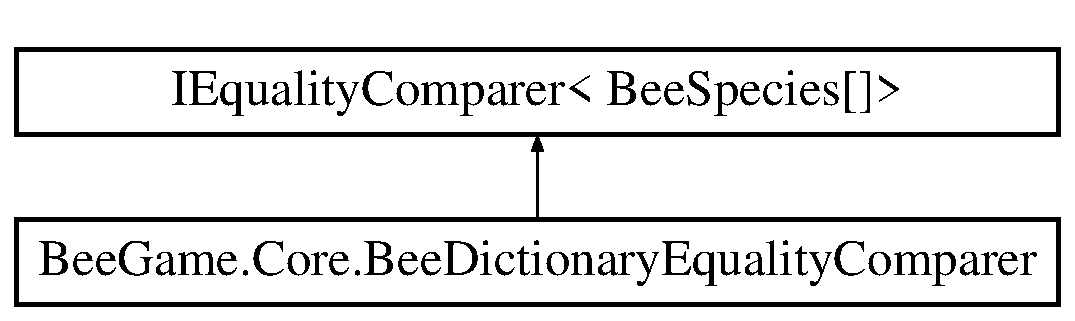
\includegraphics[height=2.000000cm]{class_bee_game_1_1_core_1_1_bee_dictionary_equality_comparer}
\end{center}
\end{figure}
\subsection*{Public Member Functions}
\begin{DoxyCompactItemize}
\item 
bool \hyperlink{class_bee_game_1_1_core_1_1_bee_dictionary_equality_comparer_a04027b45a04e74e25840b185a17c8cba}{Equals} (\hyperlink{namespace_bee_game_1_1_enums_aa2ead984825678d83c42d48f6382619c}{Bee\+Species}\mbox{[}$\,$\mbox{]} x, \hyperlink{namespace_bee_game_1_1_enums_aa2ead984825678d83c42d48f6382619c}{Bee\+Species}\mbox{[}$\,$\mbox{]} y)
\item 
int \hyperlink{class_bee_game_1_1_core_1_1_bee_dictionary_equality_comparer_acf4f3631aea262ea22aee9eaaffba8f4}{Get\+Hash\+Code} (\hyperlink{namespace_bee_game_1_1_enums_aa2ead984825678d83c42d48f6382619c}{Bee\+Species}\mbox{[}$\,$\mbox{]} obj)
\end{DoxyCompactItemize}


\subsection{Detailed Description}


Definition at line 7 of file Bee\+Dictionary\+Equality\+Comparer.\+cs.



\subsection{Member Function Documentation}
\mbox{\Hypertarget{class_bee_game_1_1_core_1_1_bee_dictionary_equality_comparer_a04027b45a04e74e25840b185a17c8cba}\label{class_bee_game_1_1_core_1_1_bee_dictionary_equality_comparer_a04027b45a04e74e25840b185a17c8cba}} 
\index{Bee\+Game\+::\+Core\+::\+Bee\+Dictionary\+Equality\+Comparer@{Bee\+Game\+::\+Core\+::\+Bee\+Dictionary\+Equality\+Comparer}!Equals@{Equals}}
\index{Equals@{Equals}!Bee\+Game\+::\+Core\+::\+Bee\+Dictionary\+Equality\+Comparer@{Bee\+Game\+::\+Core\+::\+Bee\+Dictionary\+Equality\+Comparer}}
\subsubsection{\texorpdfstring{Equals()}{Equals()}}
{\footnotesize\ttfamily bool Bee\+Game.\+Core.\+Bee\+Dictionary\+Equality\+Comparer.\+Equals (\begin{DoxyParamCaption}\item[{\hyperlink{namespace_bee_game_1_1_enums_aa2ead984825678d83c42d48f6382619c}{Bee\+Species} \mbox{[}$\,$\mbox{]}}]{x,  }\item[{\hyperlink{namespace_bee_game_1_1_enums_aa2ead984825678d83c42d48f6382619c}{Bee\+Species} \mbox{[}$\,$\mbox{]}}]{y }\end{DoxyParamCaption})}



Definition at line 9 of file Bee\+Dictionary\+Equality\+Comparer.\+cs.


\begin{DoxyCode}
10         \{
11             \textcolor{keywordflow}{if}(x.Contains(y[0]) && x.Contains(y[1]))
12             \{
13                 \textcolor{keywordflow}{return} \textcolor{keyword}{true};
14             \}
15 
16             \textcolor{keywordflow}{if}(x.Length != y.Length)
17             \{
18                 \textcolor{keywordflow}{return} \textcolor{keyword}{false};
19             \}
20             
21             \textcolor{keywordflow}{if}(x.Intersect(y).Count() == x.Length)
22             \{
23                 \textcolor{keywordflow}{return} \textcolor{keyword}{true};
24             \}
25 
26             \textcolor{keywordflow}{return} \textcolor{keyword}{false};
27         \}
\end{DoxyCode}
\mbox{\Hypertarget{class_bee_game_1_1_core_1_1_bee_dictionary_equality_comparer_acf4f3631aea262ea22aee9eaaffba8f4}\label{class_bee_game_1_1_core_1_1_bee_dictionary_equality_comparer_acf4f3631aea262ea22aee9eaaffba8f4}} 
\index{Bee\+Game\+::\+Core\+::\+Bee\+Dictionary\+Equality\+Comparer@{Bee\+Game\+::\+Core\+::\+Bee\+Dictionary\+Equality\+Comparer}!Get\+Hash\+Code@{Get\+Hash\+Code}}
\index{Get\+Hash\+Code@{Get\+Hash\+Code}!Bee\+Game\+::\+Core\+::\+Bee\+Dictionary\+Equality\+Comparer@{Bee\+Game\+::\+Core\+::\+Bee\+Dictionary\+Equality\+Comparer}}
\subsubsection{\texorpdfstring{Get\+Hash\+Code()}{GetHashCode()}}
{\footnotesize\ttfamily int Bee\+Game.\+Core.\+Bee\+Dictionary\+Equality\+Comparer.\+Get\+Hash\+Code (\begin{DoxyParamCaption}\item[{\hyperlink{namespace_bee_game_1_1_enums_aa2ead984825678d83c42d48f6382619c}{Bee\+Species} \mbox{[}$\,$\mbox{]}}]{obj }\end{DoxyParamCaption})}



Definition at line 29 of file Bee\+Dictionary\+Equality\+Comparer.\+cs.


\begin{DoxyCode}
30         \{
31             unchecked
32             \{
33                 \textcolor{keywordtype}{int} hashcode = 13;
34 
35                 \textcolor{keywordflow}{for}(\textcolor{keywordtype}{int} i = 0; i < obj.Length; i++)
36                 \{
37                     hashcode += (int)obj[i];
38                 \}
39 
40                 \textcolor{keywordflow}{return} hashcode;
41             \}
42         \}
\end{DoxyCode}


The documentation for this class was generated from the following file\+:\begin{DoxyCompactItemize}
\item 
C\+:/\+Users/\+Toothless/\+Documents/\+Git\+Hub/\+Bee\+Game/\+Code/\+Bee\+Game/\+Bee\+Game/\+Core/\hyperlink{_bee_dictionary_equality_comparer_8cs}{Bee\+Dictionary\+Equality\+Comparer.\+cs}\end{DoxyCompactItemize}

\hypertarget{class_bee_game_1_1_core_1_1_bee_dictionarys}{}\section{Bee\+Game.\+Core.\+Bee\+Dictionarys Class Reference}
\label{class_bee_game_1_1_core_1_1_bee_dictionarys}\index{Bee\+Game.\+Core.\+Bee\+Dictionarys@{Bee\+Game.\+Core.\+Bee\+Dictionarys}}


 


\subsection*{Static Public Member Functions}
\begin{DoxyCompactItemize}
\item 
static \hyperlink{struct_bee_game_1_1_bee_1_1_bee_data}{Bee\+Data} \hyperlink{class_bee_game_1_1_core_1_1_bee_dictionarys_acc616a791a2b14382dbff21433551596}{Get\+Default\+Bee\+Data} (\hyperlink{namespace_bee_game_1_1_enums_aa2ead984825678d83c42d48f6382619c}{Bee\+Species} bee\+Species)
\begin{DoxyCompactList}\small\item\em Returns the default bee data for a given species \end{DoxyCompactList}\item 
static \hyperlink{namespace_bee_game_1_1_enums_aa2ead984825678d83c42d48f6382619c}{Bee\+Species} \mbox{[}$\,$\mbox{]} \hyperlink{class_bee_game_1_1_core_1_1_bee_dictionarys_ac2d555d589392daf8d2919b6bf1fbad1}{Get\+Combination} (\hyperlink{namespace_bee_game_1_1_enums_aa2ead984825678d83c42d48f6382619c}{Bee\+Species} species1, \hyperlink{namespace_bee_game_1_1_enums_aa2ead984825678d83c42d48f6382619c}{Bee\+Species} species2)
\item 
static float \hyperlink{class_bee_game_1_1_core_1_1_bee_dictionarys_adb5fe5760a94dbff606bc1d20ee67aaa}{Get\+Mutation\+Chance} (\hyperlink{namespace_bee_game_1_1_enums_aa2ead984825678d83c42d48f6382619c}{Bee\+Species} species)
\item 
static float \mbox{[}$\,$\mbox{]} \hyperlink{class_bee_game_1_1_core_1_1_bee_dictionarys_ae563db005a03a49d25cb6cdbd4d3a82e}{Get\+Mutation\+Chance} (\hyperlink{namespace_bee_game_1_1_enums_aa2ead984825678d83c42d48f6382619c}{Bee\+Species}\mbox{[}$\,$\mbox{]} species)
\begin{DoxyCompactList}\small\item\em Returns the mutation chances for each of the Bee\+Species\mbox{[}$\,$\mbox{]} that are given. Returns values in the same order they are given \end{DoxyCompactList}\item 
static \hyperlink{struct_bee_game_1_1_items_1_1_item}{Item} \mbox{[}$\,$\mbox{]} \hyperlink{class_bee_game_1_1_core_1_1_bee_dictionarys_a2cd137701cfdcfeb25d5e7a73397e1b4}{Get\+Items} (\hyperlink{namespace_bee_game_1_1_enums_aa2ead984825678d83c42d48f6382619c}{Bee\+Species} species)
\end{DoxyCompactItemize}
\subsection*{Static Private Attributes}
\begin{DoxyCompactItemize}
\item 
static Dictionary$<$ \hyperlink{namespace_bee_game_1_1_enums_aa2ead984825678d83c42d48f6382619c}{Bee\+Species}, \hyperlink{struct_bee_game_1_1_bee_1_1_bee_data}{Bee\+Data} $>$ \hyperlink{class_bee_game_1_1_core_1_1_bee_dictionarys_a4bd3dbe3fc155e206801656c07212a96}{bee\+Default\+Data}
\begin{DoxyCompactList}\small\item\em Contains the default data for all the bee species, this will then be edited in the alveary/apiary according to the bees it is combined with \end{DoxyCompactList}\item 
static Dictionary$<$ \hyperlink{namespace_bee_game_1_1_enums_aa2ead984825678d83c42d48f6382619c}{Bee\+Species}\mbox{[}$\,$\mbox{]}, \hyperlink{namespace_bee_game_1_1_enums_aa2ead984825678d83c42d48f6382619c}{Bee\+Species}\mbox{[}$\,$\mbox{]}$>$ \hyperlink{class_bee_game_1_1_core_1_1_bee_dictionarys_a1ebc1dfba158d134ff8b28082c9a2cb2}{bee\+Combinations}
\item 
static Dictionary$<$ \hyperlink{namespace_bee_game_1_1_enums_aa2ead984825678d83c42d48f6382619c}{Bee\+Species}, float $>$ \hyperlink{class_bee_game_1_1_core_1_1_bee_dictionarys_a8928aea7b0d5b04fbf7b5055a9921385}{bee\+Mutation\+Chance}
\item 
static Dictionary$<$ \hyperlink{namespace_bee_game_1_1_enums_aa2ead984825678d83c42d48f6382619c}{Bee\+Species}, \hyperlink{struct_bee_game_1_1_items_1_1_item}{Item}\mbox{[}$\,$\mbox{]}$>$ \hyperlink{class_bee_game_1_1_core_1_1_bee_dictionarys_a08901f100e7fa17a7a441b32ec680146}{items}
\end{DoxyCompactItemize}


\subsection{Detailed Description}


\begin{DoxyRefDesc}{Todo}
\item[\hyperlink{todo__todo000004}{Todo}]add summary tags to all dictionarys \end{DoxyRefDesc}


Definition at line 12 of file Bee\+Dictionarys.\+cs.



\subsection{Member Function Documentation}
\mbox{\Hypertarget{class_bee_game_1_1_core_1_1_bee_dictionarys_ac2d555d589392daf8d2919b6bf1fbad1}\label{class_bee_game_1_1_core_1_1_bee_dictionarys_ac2d555d589392daf8d2919b6bf1fbad1}} 
\index{Bee\+Game\+::\+Core\+::\+Bee\+Dictionarys@{Bee\+Game\+::\+Core\+::\+Bee\+Dictionarys}!Get\+Combination@{Get\+Combination}}
\index{Get\+Combination@{Get\+Combination}!Bee\+Game\+::\+Core\+::\+Bee\+Dictionarys@{Bee\+Game\+::\+Core\+::\+Bee\+Dictionarys}}
\subsubsection{\texorpdfstring{Get\+Combination()}{GetCombination()}}
{\footnotesize\ttfamily static \hyperlink{namespace_bee_game_1_1_enums_aa2ead984825678d83c42d48f6382619c}{Bee\+Species} \mbox{[}$\,$\mbox{]} Bee\+Game.\+Core.\+Bee\+Dictionarys.\+Get\+Combination (\begin{DoxyParamCaption}\item[{\hyperlink{namespace_bee_game_1_1_enums_aa2ead984825678d83c42d48f6382619c}{Bee\+Species}}]{species1,  }\item[{\hyperlink{namespace_bee_game_1_1_enums_aa2ead984825678d83c42d48f6382619c}{Bee\+Species}}]{species2 }\end{DoxyParamCaption})\hspace{0.3cm}{\ttfamily [static]}}



Definition at line 50 of file Bee\+Dictionarys.\+cs.


\begin{DoxyCode}
51         \{
52             \hyperlink{namespace_bee_game_1_1_enums_aa2ead984825678d83c42d48f6382619c}{BeeSpecies}[] speciesArray = \textcolor{keyword}{new} \hyperlink{namespace_bee_game_1_1_enums_aa2ead984825678d83c42d48f6382619c}{BeeSpecies}[2] \{ species1, species2 \};
53 
54             \hyperlink{namespace_bee_game_1_1_enums_aa2ead984825678d83c42d48f6382619c}{BeeSpecies}[][] keyss = \hyperlink{class_bee_game_1_1_core_1_1_bee_dictionarys_a1ebc1dfba158d134ff8b28082c9a2cb2}{beeCombinations}.Keys.ToArray();
55             BeeDictionaryEqualityComparer comp = \textcolor{keyword}{new} BeeDictionaryEqualityComparer();
56 
57             \textcolor{keywordflow}{for} (\textcolor{keywordtype}{int} i = 0; i < keyss.Length; i++)
58             \{
59                 \textcolor{keywordflow}{if}(comp.Equals(keyss[i], speciesArray))
60                 \{
61                     \textcolor{keywordflow}{return} \hyperlink{class_bee_game_1_1_core_1_1_bee_dictionarys_a1ebc1dfba158d134ff8b28082c9a2cb2}{beeCombinations}[keyss[i]];
62                 \}
63             \}
64 
65             \textcolor{keywordflow}{return} null;
66         \}
\end{DoxyCode}
\mbox{\Hypertarget{class_bee_game_1_1_core_1_1_bee_dictionarys_acc616a791a2b14382dbff21433551596}\label{class_bee_game_1_1_core_1_1_bee_dictionarys_acc616a791a2b14382dbff21433551596}} 
\index{Bee\+Game\+::\+Core\+::\+Bee\+Dictionarys@{Bee\+Game\+::\+Core\+::\+Bee\+Dictionarys}!Get\+Default\+Bee\+Data@{Get\+Default\+Bee\+Data}}
\index{Get\+Default\+Bee\+Data@{Get\+Default\+Bee\+Data}!Bee\+Game\+::\+Core\+::\+Bee\+Dictionarys@{Bee\+Game\+::\+Core\+::\+Bee\+Dictionarys}}
\subsubsection{\texorpdfstring{Get\+Default\+Bee\+Data()}{GetDefaultBeeData()}}
{\footnotesize\ttfamily static \hyperlink{struct_bee_game_1_1_bee_1_1_bee_data}{Bee\+Data} Bee\+Game.\+Core.\+Bee\+Dictionarys.\+Get\+Default\+Bee\+Data (\begin{DoxyParamCaption}\item[{\hyperlink{namespace_bee_game_1_1_enums_aa2ead984825678d83c42d48f6382619c}{Bee\+Species}}]{bee\+Species }\end{DoxyParamCaption})\hspace{0.3cm}{\ttfamily [static]}}



Returns the default bee data for a given species 


\begin{DoxyParams}{Parameters}
{\em bee\+Species} & Bee\+Species\\
\hline
\end{DoxyParams}
\begin{DoxyReturn}{Returns}
Returns the default Bee\+Data for the given species
\end{DoxyReturn}


Definition at line 29 of file Bee\+Dictionarys.\+cs.


\begin{DoxyCode}
30         \{
31             \textcolor{keywordflow}{if} (\hyperlink{class_bee_game_1_1_core_1_1_bee_dictionarys_a4bd3dbe3fc155e206801656c07212a96}{beeDefaultData}.ContainsKey(beeSpecies))
32             \{
33                 \hyperlink{struct_bee_game_1_1_bee_1_1_bee_data}{BeeData} bee = \textcolor{keyword}{new} \hyperlink{struct_bee_game_1_1_bee_1_1_bee_data}{BeeData}(\hyperlink{class_bee_game_1_1_core_1_1_bee_dictionarys_a4bd3dbe3fc155e206801656c07212a96}{beeDefaultData}[beeSpecies]);
34                 \textcolor{keywordflow}{return} bee;
35             \}
36             \textcolor{keywordflow}{else}
37             \{
38                 \textcolor{keywordflow}{return} null;
39             \}
40         \}
\end{DoxyCode}
\mbox{\Hypertarget{class_bee_game_1_1_core_1_1_bee_dictionarys_a2cd137701cfdcfeb25d5e7a73397e1b4}\label{class_bee_game_1_1_core_1_1_bee_dictionarys_a2cd137701cfdcfeb25d5e7a73397e1b4}} 
\index{Bee\+Game\+::\+Core\+::\+Bee\+Dictionarys@{Bee\+Game\+::\+Core\+::\+Bee\+Dictionarys}!Get\+Items@{Get\+Items}}
\index{Get\+Items@{Get\+Items}!Bee\+Game\+::\+Core\+::\+Bee\+Dictionarys@{Bee\+Game\+::\+Core\+::\+Bee\+Dictionarys}}
\subsubsection{\texorpdfstring{Get\+Items()}{GetItems()}}
{\footnotesize\ttfamily static \hyperlink{struct_bee_game_1_1_items_1_1_item}{Item} \mbox{[}$\,$\mbox{]} Bee\+Game.\+Core.\+Bee\+Dictionarys.\+Get\+Items (\begin{DoxyParamCaption}\item[{\hyperlink{namespace_bee_game_1_1_enums_aa2ead984825678d83c42d48f6382619c}{Bee\+Species}}]{species }\end{DoxyParamCaption})\hspace{0.3cm}{\ttfamily [static]}}



Definition at line 123 of file Bee\+Dictionarys.\+cs.


\begin{DoxyCode}
124         \{
125             \textcolor{keywordflow}{return} \hyperlink{class_bee_game_1_1_core_1_1_bee_dictionarys_a08901f100e7fa17a7a441b32ec680146}{items}[species];
126         \}
\end{DoxyCode}
\mbox{\Hypertarget{class_bee_game_1_1_core_1_1_bee_dictionarys_adb5fe5760a94dbff606bc1d20ee67aaa}\label{class_bee_game_1_1_core_1_1_bee_dictionarys_adb5fe5760a94dbff606bc1d20ee67aaa}} 
\index{Bee\+Game\+::\+Core\+::\+Bee\+Dictionarys@{Bee\+Game\+::\+Core\+::\+Bee\+Dictionarys}!Get\+Mutation\+Chance@{Get\+Mutation\+Chance}}
\index{Get\+Mutation\+Chance@{Get\+Mutation\+Chance}!Bee\+Game\+::\+Core\+::\+Bee\+Dictionarys@{Bee\+Game\+::\+Core\+::\+Bee\+Dictionarys}}
\subsubsection{\texorpdfstring{Get\+Mutation\+Chance()}{GetMutationChance()}\hspace{0.1cm}{\footnotesize\ttfamily [1/2]}}
{\footnotesize\ttfamily static float Bee\+Game.\+Core.\+Bee\+Dictionarys.\+Get\+Mutation\+Chance (\begin{DoxyParamCaption}\item[{\hyperlink{namespace_bee_game_1_1_enums_aa2ead984825678d83c42d48f6382619c}{Bee\+Species}}]{species }\end{DoxyParamCaption})\hspace{0.3cm}{\ttfamily [static]}}



Definition at line 76 of file Bee\+Dictionarys.\+cs.


\begin{DoxyCode}
77         \{
78             \textcolor{keywordflow}{if}(\hyperlink{class_bee_game_1_1_core_1_1_bee_dictionarys_a8928aea7b0d5b04fbf7b5055a9921385}{beeMutationChance}.ContainsKey(species))
79             \{
80                 \textcolor{keywordflow}{return} \hyperlink{class_bee_game_1_1_core_1_1_bee_dictionarys_a8928aea7b0d5b04fbf7b5055a9921385}{beeMutationChance}[species];
81             \}
82             \textcolor{keywordflow}{else}
83             \{
84                 \textcolor{keywordflow}{return} 1f;
85             \}
86         \}
\end{DoxyCode}
\mbox{\Hypertarget{class_bee_game_1_1_core_1_1_bee_dictionarys_ae563db005a03a49d25cb6cdbd4d3a82e}\label{class_bee_game_1_1_core_1_1_bee_dictionarys_ae563db005a03a49d25cb6cdbd4d3a82e}} 
\index{Bee\+Game\+::\+Core\+::\+Bee\+Dictionarys@{Bee\+Game\+::\+Core\+::\+Bee\+Dictionarys}!Get\+Mutation\+Chance@{Get\+Mutation\+Chance}}
\index{Get\+Mutation\+Chance@{Get\+Mutation\+Chance}!Bee\+Game\+::\+Core\+::\+Bee\+Dictionarys@{Bee\+Game\+::\+Core\+::\+Bee\+Dictionarys}}
\subsubsection{\texorpdfstring{Get\+Mutation\+Chance()}{GetMutationChance()}\hspace{0.1cm}{\footnotesize\ttfamily [2/2]}}
{\footnotesize\ttfamily static float \mbox{[}$\,$\mbox{]} Bee\+Game.\+Core.\+Bee\+Dictionarys.\+Get\+Mutation\+Chance (\begin{DoxyParamCaption}\item[{\hyperlink{namespace_bee_game_1_1_enums_aa2ead984825678d83c42d48f6382619c}{Bee\+Species} \mbox{[}$\,$\mbox{]}}]{species }\end{DoxyParamCaption})\hspace{0.3cm}{\ttfamily [static]}}



Returns the mutation chances for each of the Bee\+Species\mbox{[}$\,$\mbox{]} that are given. Returns values in the same order they are given 


\begin{DoxyParams}{Parameters}
{\em species} & Bee\+Species that the mutation chances are required for\\
\hline
\end{DoxyParams}
\begin{DoxyReturn}{Returns}
Return null if the Bee\+Species is not in the \hyperlink{class_bee_game_1_1_core_1_1_bee_dictionarys_a8928aea7b0d5b04fbf7b5055a9921385}{bee\+Mutation\+Chance} dictionary else it will return the mutation chances as a float array
\end{DoxyReturn}


Definition at line 93 of file Bee\+Dictionarys.\+cs.


\begin{DoxyCode}
94         \{
95             \textcolor{keywordflow}{for} (\textcolor{keywordtype}{int} i = 0; i < species.Length; i++)
96             \{
97                 \textcolor{keywordflow}{if}(!\hyperlink{class_bee_game_1_1_core_1_1_bee_dictionarys_a8928aea7b0d5b04fbf7b5055a9921385}{beeMutationChance}.ContainsKey(species[i]))
98                 \{
99                     \textcolor{keywordflow}{return} null;
100                 \}
101             \}
102 
103             \textcolor{keywordtype}{float}[] returnValues = \textcolor{keyword}{new} \textcolor{keywordtype}{float}[species.Length];
104 
105             \textcolor{keywordflow}{for} (\textcolor{keywordtype}{int} i = 0; i < species.Length; i++)
106             \{
107                 returnValues[i] = \hyperlink{class_bee_game_1_1_core_1_1_bee_dictionarys_a8928aea7b0d5b04fbf7b5055a9921385}{beeMutationChance}[species[i]];
108             \}
109 
110             \textcolor{keywordflow}{return} returnValues;
111         \}
\end{DoxyCode}


\subsection{Member Data Documentation}
\mbox{\Hypertarget{class_bee_game_1_1_core_1_1_bee_dictionarys_a1ebc1dfba158d134ff8b28082c9a2cb2}\label{class_bee_game_1_1_core_1_1_bee_dictionarys_a1ebc1dfba158d134ff8b28082c9a2cb2}} 
\index{Bee\+Game\+::\+Core\+::\+Bee\+Dictionarys@{Bee\+Game\+::\+Core\+::\+Bee\+Dictionarys}!bee\+Combinations@{bee\+Combinations}}
\index{bee\+Combinations@{bee\+Combinations}!Bee\+Game\+::\+Core\+::\+Bee\+Dictionarys@{Bee\+Game\+::\+Core\+::\+Bee\+Dictionarys}}
\subsubsection{\texorpdfstring{bee\+Combinations}{beeCombinations}}
{\footnotesize\ttfamily Dictionary$<$\hyperlink{namespace_bee_game_1_1_enums_aa2ead984825678d83c42d48f6382619c}{Bee\+Species}\mbox{[}$\,$\mbox{]}, \hyperlink{namespace_bee_game_1_1_enums_aa2ead984825678d83c42d48f6382619c}{Bee\+Species}\mbox{[}$\,$\mbox{]}$>$ Bee\+Game.\+Core.\+Bee\+Dictionarys.\+bee\+Combinations\hspace{0.3cm}{\ttfamily [static]}, {\ttfamily [private]}}

{\bfseries Initial value\+:}
\begin{DoxyCode}
= \textcolor{keyword}{new} Dictionary<BeeSpecies[], BeeSpecies[]>(\textcolor{keyword}{new} BeeDictionaryEqualityComparer())
        \{
            \{\textcolor{keyword}{new} \hyperlink{namespace_bee_game_1_1_enums_aa2ead984825678d83c42d48f6382619c}{BeeSpecies}[6] \{\hyperlink{namespace_bee_game_1_1_enums_aa2ead984825678d83c42d48f6382619c}{BeeSpecies}.FOREST, 
      \hyperlink{namespace_bee_game_1_1_enums_aa2ead984825678d83c42d48f6382619c}{BeeSpecies}.MEADOWS, \hyperlink{namespace_bee_game_1_1_enums_aa2ead984825678d83c42d48f6382619c}{BeeSpecies}.TROPICAL, \hyperlink{namespace_bee_game_1_1_enums_aa2ead984825678d83c42d48f6382619c}{BeeSpecies}.WINTRY, 
      \hyperlink{namespace_bee_game_1_1_enums_aa2ead984825678d83c42d48f6382619c}{BeeSpecies}.MODEST, \hyperlink{namespace_bee_game_1_1_enums_aa2ead984825678d83c42d48f6382619c}{BeeSpecies}.MARSHY\}, \textcolor{keyword}{new} \hyperlink{namespace_bee_game_1_1_enums_aa2ead984825678d83c42d48f6382619c}{BeeSpecies}[1] \{
      \hyperlink{namespace_bee_game_1_1_enums_aa2ead984825678d83c42d48f6382619c}{BeeSpecies}.COMMON\} \},
            \{\textcolor{keyword}{new} \hyperlink{namespace_bee_game_1_1_enums_aa2ead984825678d83c42d48f6382619c}{BeeSpecies}[2] \{\hyperlink{namespace_bee_game_1_1_enums_aa2ead984825678d83c42d48f6382619c}{BeeSpecies}.SETADFAST, 
      \hyperlink{namespace_bee_game_1_1_enums_aa2ead984825678d83c42d48f6382619c}{BeeSpecies}.VALIANT\}, \textcolor{keyword}{new} \hyperlink{namespace_bee_game_1_1_enums_aa2ead984825678d83c42d48f6382619c}{BeeSpecies}[1] \{\hyperlink{namespace_bee_game_1_1_enums_aa2ead984825678d83c42d48f6382619c}{BeeSpecies}.HEROIC\} \}
        \}
\end{DoxyCode}


Definition at line 44 of file Bee\+Dictionarys.\+cs.

\mbox{\Hypertarget{class_bee_game_1_1_core_1_1_bee_dictionarys_a4bd3dbe3fc155e206801656c07212a96}\label{class_bee_game_1_1_core_1_1_bee_dictionarys_a4bd3dbe3fc155e206801656c07212a96}} 
\index{Bee\+Game\+::\+Core\+::\+Bee\+Dictionarys@{Bee\+Game\+::\+Core\+::\+Bee\+Dictionarys}!bee\+Default\+Data@{bee\+Default\+Data}}
\index{bee\+Default\+Data@{bee\+Default\+Data}!Bee\+Game\+::\+Core\+::\+Bee\+Dictionarys@{Bee\+Game\+::\+Core\+::\+Bee\+Dictionarys}}
\subsubsection{\texorpdfstring{bee\+Default\+Data}{beeDefaultData}}
{\footnotesize\ttfamily Dictionary$<$\hyperlink{namespace_bee_game_1_1_enums_aa2ead984825678d83c42d48f6382619c}{Bee\+Species}, \hyperlink{struct_bee_game_1_1_bee_1_1_bee_data}{Bee\+Data}$>$ Bee\+Game.\+Core.\+Bee\+Dictionarys.\+bee\+Default\+Data\hspace{0.3cm}{\ttfamily [static]}, {\ttfamily [private]}}

{\bfseries Initial value\+:}
\begin{DoxyCode}
= \textcolor{keyword}{new} Dictionary<BeeSpecies, BeeData>()
        \{
            \{ \hyperlink{namespace_bee_game_1_1_enums_aa2ead984825678d83c42d48f6382619c}{BeeSpecies}.FOREST, \textcolor{keyword}{new} BeeData \{pSpecies = \hyperlink{namespace_bee_game_1_1_enums_aa2ead984825678d83c42d48f6382619c}{BeeSpecies}.FOREST, pLifespan =
       \hyperlink{namespace_bee_game_1_1_enums_ae3853807ded2f4d99a0d4a7fb4b2bc46}{BeeLifeSpan}.NORMAL, pFertility = 3, pEffect = \hyperlink{namespace_bee_game_1_1_enums_acf7ae32a86385a40fc0c7b55af95c6c3}{BeeEffect}.NONE, pProdSpeed = 
      \hyperlink{namespace_bee_game_1_1_enums_afee18200a21cc4b8e1d0cdb669930f14}{BeeProductionSpeed}.NORMAL, tempPref = \hyperlink{namespace_bee_game_1_1_enums_a9db0f9ac859fab168654d657f248b024}{BeeTempPreferance}.TEMPERATE, 
      tempTol = \textcolor{keyword}{new} \textcolor{keywordtype}{int}[] \{-1, 1\}, humidPref = \hyperlink{namespace_bee_game_1_1_enums_a66566cbc9da8d1d1e402156b4bd3bf9d}{BeeHumidityPreferance}.TEMPERATE, humidTol = \textcolor{keyword}{new} \textcolor{keywordtype}{int}
      [] \{-1, 1\}, nocturnal = \textcolor{keyword}{false}, flyer = \textcolor{keyword}{false}\} \},
            \{ \hyperlink{namespace_bee_game_1_1_enums_aa2ead984825678d83c42d48f6382619c}{BeeSpecies}.MEADOWS, \textcolor{keyword}{new} BeeData \{pSpecies = \hyperlink{namespace_bee_game_1_1_enums_aa2ead984825678d83c42d48f6382619c}{BeeSpecies}.MEADOWS, pLifespan
       = \hyperlink{namespace_bee_game_1_1_enums_ae3853807ded2f4d99a0d4a7fb4b2bc46}{BeeLifeSpan}.NORMAL, pFertility = 3, pEffect = \hyperlink{namespace_bee_game_1_1_enums_acf7ae32a86385a40fc0c7b55af95c6c3}{BeeEffect}.NONE, pProdSpeed = 
      \hyperlink{namespace_bee_game_1_1_enums_afee18200a21cc4b8e1d0cdb669930f14}{BeeProductionSpeed}.NORMAL, tempPref = \hyperlink{namespace_bee_game_1_1_enums_a9db0f9ac859fab168654d657f248b024}{BeeTempPreferance}.TEMPERATE, 
      tempTol = \textcolor{keyword}{new} \textcolor{keywordtype}{int}[] \{-1, 1\}, humidPref = \hyperlink{namespace_bee_game_1_1_enums_a66566cbc9da8d1d1e402156b4bd3bf9d}{BeeHumidityPreferance}.TEMPERATE, humidTol = \textcolor{keyword}{new} \textcolor{keywordtype}{int}
      [] \{-1, 1\}, nocturnal = \textcolor{keyword}{false}, flyer = \textcolor{keyword}{false}\} \}
        \}
\end{DoxyCode}


Contains the default data for all the bee species, this will then be edited in the alveary/apiary according to the bees it is combined with 



Definition at line 18 of file Bee\+Dictionarys.\+cs.

\mbox{\Hypertarget{class_bee_game_1_1_core_1_1_bee_dictionarys_a8928aea7b0d5b04fbf7b5055a9921385}\label{class_bee_game_1_1_core_1_1_bee_dictionarys_a8928aea7b0d5b04fbf7b5055a9921385}} 
\index{Bee\+Game\+::\+Core\+::\+Bee\+Dictionarys@{Bee\+Game\+::\+Core\+::\+Bee\+Dictionarys}!bee\+Mutation\+Chance@{bee\+Mutation\+Chance}}
\index{bee\+Mutation\+Chance@{bee\+Mutation\+Chance}!Bee\+Game\+::\+Core\+::\+Bee\+Dictionarys@{Bee\+Game\+::\+Core\+::\+Bee\+Dictionarys}}
\subsubsection{\texorpdfstring{bee\+Mutation\+Chance}{beeMutationChance}}
{\footnotesize\ttfamily Dictionary$<$\hyperlink{namespace_bee_game_1_1_enums_aa2ead984825678d83c42d48f6382619c}{Bee\+Species}, float$>$ Bee\+Game.\+Core.\+Bee\+Dictionarys.\+bee\+Mutation\+Chance\hspace{0.3cm}{\ttfamily [static]}, {\ttfamily [private]}}

{\bfseries Initial value\+:}
\begin{DoxyCode}
= \textcolor{keyword}{new} Dictionary<BeeSpecies, float>()
        \{
            \{\hyperlink{namespace_bee_game_1_1_enums_aa2ead984825678d83c42d48f6382619c}{BeeSpecies}.COMMON, 0.15f \},
            \{\hyperlink{namespace_bee_game_1_1_enums_aa2ead984825678d83c42d48f6382619c}{BeeSpecies}.HEROIC, 0.06f \}
        \}
\end{DoxyCode}


Definition at line 70 of file Bee\+Dictionarys.\+cs.

\mbox{\Hypertarget{class_bee_game_1_1_core_1_1_bee_dictionarys_a08901f100e7fa17a7a441b32ec680146}\label{class_bee_game_1_1_core_1_1_bee_dictionarys_a08901f100e7fa17a7a441b32ec680146}} 
\index{Bee\+Game\+::\+Core\+::\+Bee\+Dictionarys@{Bee\+Game\+::\+Core\+::\+Bee\+Dictionarys}!items@{items}}
\index{items@{items}!Bee\+Game\+::\+Core\+::\+Bee\+Dictionarys@{Bee\+Game\+::\+Core\+::\+Bee\+Dictionarys}}
\subsubsection{\texorpdfstring{items}{items}}
{\footnotesize\ttfamily Dictionary$<$\hyperlink{namespace_bee_game_1_1_enums_aa2ead984825678d83c42d48f6382619c}{Bee\+Species}, \hyperlink{struct_bee_game_1_1_items_1_1_item}{Item}\mbox{[}$\,$\mbox{]}$>$ Bee\+Game.\+Core.\+Bee\+Dictionarys.\+items\hspace{0.3cm}{\ttfamily [static]}, {\ttfamily [private]}}

{\bfseries Initial value\+:}
\begin{DoxyCode}
= \textcolor{keyword}{new} Dictionary<BeeSpecies, Item[]>()
        \{
            \{\hyperlink{namespace_bee_game_1_1_enums_aa2ead984825678d83c42d48f6382619c}{BeeSpecies}.FOREST, \textcolor{keyword}{new} Item[1] \},
            \{\hyperlink{namespace_bee_game_1_1_enums_aa2ead984825678d83c42d48f6382619c}{BeeSpecies}.MEADOWS, \textcolor{keyword}{new} Item[1] \},
            \{\hyperlink{namespace_bee_game_1_1_enums_aa2ead984825678d83c42d48f6382619c}{BeeSpecies}.TROPICAL, \textcolor{keyword}{new} Item[1] \}
        \}
\end{DoxyCode}


Definition at line 115 of file Bee\+Dictionarys.\+cs.



The documentation for this class was generated from the following file\+:\begin{DoxyCompactItemize}
\item 
C\+:/\+Users/\+Toothless/\+Documents/\+Git\+Hub/\+Bee\+Game/\+Code/\+Bee\+Game/\+Bee\+Game/\+Core/\hyperlink{_bee_dictionarys_8cs}{Bee\+Dictionarys.\+cs}\end{DoxyCompactItemize}

\hypertarget{class_bee_game_1_1_blocks_1_1_block}{}\section{Bee\+Game.\+Blocks.\+Block Class Reference}
\label{class_bee_game_1_1_blocks_1_1_block}\index{Bee\+Game.\+Blocks.\+Block@{Bee\+Game.\+Blocks.\+Block}}
\subsection*{Public Member Functions}
\begin{DoxyCompactItemize}
\item 
override int \hyperlink{class_bee_game_1_1_blocks_1_1_block_a803b906cb4fcfdb10157177a1468dbac}{Get\+Hash\+Code} ()
\begin{DoxyCompactList}\small\item\em Makes c\# happy \end{DoxyCompactList}\item 
override bool \hyperlink{class_bee_game_1_1_blocks_1_1_block_a03187300c8fd940defb0dbe2793d1d83}{Equals} (object obj)
\begin{DoxyCompactList}\small\item\em Makes c\# happy \end{DoxyCompactList}\end{DoxyCompactItemize}
\subsection*{Static Public Member Functions}
\begin{DoxyCompactItemize}
\item 
static bool \hyperlink{class_bee_game_1_1_blocks_1_1_block_a620f4aba15b9280f1c659dc4557f8cd8}{operator==} (\hyperlink{class_bee_game_1_1_blocks_1_1_block}{Block} a, \hyperlink{class_bee_game_1_1_blocks_1_1_block}{Block} b)
\begin{DoxyCompactList}\small\item\em Returns true if block a and block b have the same position \end{DoxyCompactList}\item 
static bool \hyperlink{class_bee_game_1_1_blocks_1_1_block_ac5ac088908d491883260b5c24d3caf79}{operator!=} (\hyperlink{class_bee_game_1_1_blocks_1_1_block}{Block} a, \hyperlink{class_bee_game_1_1_blocks_1_1_block}{Block} b)
\begin{DoxyCompactList}\small\item\em Retuns inverse of == \end{DoxyCompactList}\end{DoxyCompactItemize}
\subsection*{Public Attributes}
\begin{DoxyCompactItemize}
\item 
\hyperlink{struct_bee_game_1_1_items_1_1_item}{Item} \hyperlink{class_bee_game_1_1_blocks_1_1_block_addc8d61c8acab21b0f15df5fed804f11}{item}
\begin{DoxyCompactList}\small\item\em Item that this block is \end{DoxyCompactList}\item 
\hyperlink{struct_bee_game_1_1_t_h_vector3}{T\+H\+Vector3} \hyperlink{class_bee_game_1_1_blocks_1_1_block_a4bdeec76cfc1291eab6cebcd569620e6}{position}
\begin{DoxyCompactList}\small\item\em Objects positon as a \hyperlink{struct_bee_game_1_1_t_h_vector3}{T\+H\+Vector3} \end{DoxyCompactList}\item 
\hyperlink{struct_bee_game_1_1_items_1_1_item}{Item} \mbox{[}$\,$\mbox{]} \hyperlink{class_bee_game_1_1_blocks_1_1_block_a54846c7c7ec2f512484b3060de977fac}{inventory\+Items}
\begin{DoxyCompactList}\small\item\em \hyperlink{namespace_bee_game_1_1_items}{Items} in this blocks inventory (may not be used) \end{DoxyCompactList}\end{DoxyCompactItemize}


\subsection{Detailed Description}


Definition at line 9 of file Block.\+cs.



\subsection{Member Function Documentation}
\mbox{\Hypertarget{class_bee_game_1_1_blocks_1_1_block_a03187300c8fd940defb0dbe2793d1d83}\label{class_bee_game_1_1_blocks_1_1_block_a03187300c8fd940defb0dbe2793d1d83}} 
\index{Bee\+Game\+::\+Blocks\+::\+Block@{Bee\+Game\+::\+Blocks\+::\+Block}!Equals@{Equals}}
\index{Equals@{Equals}!Bee\+Game\+::\+Blocks\+::\+Block@{Bee\+Game\+::\+Blocks\+::\+Block}}
\subsubsection{\texorpdfstring{Equals()}{Equals()}}
{\footnotesize\ttfamily override bool Bee\+Game.\+Blocks.\+Block.\+Equals (\begin{DoxyParamCaption}\item[{object}]{obj }\end{DoxyParamCaption})}



Makes c\# happy 


\begin{DoxyParams}{Parameters}
{\em obj} & Object\\
\hline
\end{DoxyParams}
\begin{DoxyReturn}{Returns}
true if object are the same
\end{DoxyReturn}


Definition at line 38 of file Block.\+cs.


\begin{DoxyCode}
39         \{
40             \textcolor{keywordflow}{return} base.Equals(obj);
41         \}
\end{DoxyCode}
\mbox{\Hypertarget{class_bee_game_1_1_blocks_1_1_block_a803b906cb4fcfdb10157177a1468dbac}\label{class_bee_game_1_1_blocks_1_1_block_a803b906cb4fcfdb10157177a1468dbac}} 
\index{Bee\+Game\+::\+Blocks\+::\+Block@{Bee\+Game\+::\+Blocks\+::\+Block}!Get\+Hash\+Code@{Get\+Hash\+Code}}
\index{Get\+Hash\+Code@{Get\+Hash\+Code}!Bee\+Game\+::\+Blocks\+::\+Block@{Bee\+Game\+::\+Blocks\+::\+Block}}
\subsubsection{\texorpdfstring{Get\+Hash\+Code()}{GetHashCode()}}
{\footnotesize\ttfamily override int Bee\+Game.\+Blocks.\+Block.\+Get\+Hash\+Code (\begin{DoxyParamCaption}{ }\end{DoxyParamCaption})}



Makes c\# happy 

\begin{DoxyReturn}{Returns}
Object Hash\+Code
\end{DoxyReturn}


Definition at line 29 of file Block.\+cs.


\begin{DoxyCode}
30         \{
31             \textcolor{keywordflow}{return} base.GetHashCode();
32         \}
\end{DoxyCode}
\mbox{\Hypertarget{class_bee_game_1_1_blocks_1_1_block_ac5ac088908d491883260b5c24d3caf79}\label{class_bee_game_1_1_blocks_1_1_block_ac5ac088908d491883260b5c24d3caf79}} 
\index{Bee\+Game\+::\+Blocks\+::\+Block@{Bee\+Game\+::\+Blocks\+::\+Block}!operator"!=@{operator"!=}}
\index{operator"!=@{operator"!=}!Bee\+Game\+::\+Blocks\+::\+Block@{Bee\+Game\+::\+Blocks\+::\+Block}}
\subsubsection{\texorpdfstring{operator"!=()}{operator!=()}}
{\footnotesize\ttfamily static bool Bee\+Game.\+Blocks.\+Block.\+operator!= (\begin{DoxyParamCaption}\item[{\hyperlink{class_bee_game_1_1_blocks_1_1_block}{Block}}]{a,  }\item[{\hyperlink{class_bee_game_1_1_blocks_1_1_block}{Block}}]{b }\end{DoxyParamCaption})\hspace{0.3cm}{\ttfamily [static]}}



Retuns inverse of == 


\begin{DoxyParams}{Parameters}
{\em a} & \hyperlink{class_bee_game_1_1_blocks_1_1_block}{Block} 1\\
\hline
{\em b} & \hyperlink{class_bee_game_1_1_blocks_1_1_block}{Block} 2\\
\hline
\end{DoxyParams}
\begin{DoxyReturn}{Returns}
Inverse if ==
\end{DoxyReturn}


Definition at line 60 of file Block.\+cs.


\begin{DoxyCode}
61         \{
62             \textcolor{keywordflow}{return} (a == b);
63         \}
\end{DoxyCode}
\mbox{\Hypertarget{class_bee_game_1_1_blocks_1_1_block_a620f4aba15b9280f1c659dc4557f8cd8}\label{class_bee_game_1_1_blocks_1_1_block_a620f4aba15b9280f1c659dc4557f8cd8}} 
\index{Bee\+Game\+::\+Blocks\+::\+Block@{Bee\+Game\+::\+Blocks\+::\+Block}!operator==@{operator==}}
\index{operator==@{operator==}!Bee\+Game\+::\+Blocks\+::\+Block@{Bee\+Game\+::\+Blocks\+::\+Block}}
\subsubsection{\texorpdfstring{operator==()}{operator==()}}
{\footnotesize\ttfamily static bool Bee\+Game.\+Blocks.\+Block.\+operator== (\begin{DoxyParamCaption}\item[{\hyperlink{class_bee_game_1_1_blocks_1_1_block}{Block}}]{a,  }\item[{\hyperlink{class_bee_game_1_1_blocks_1_1_block}{Block}}]{b }\end{DoxyParamCaption})\hspace{0.3cm}{\ttfamily [static]}}



Returns true if block a and block b have the same position 


\begin{DoxyParams}{Parameters}
{\em a} & \hyperlink{class_bee_game_1_1_blocks_1_1_block}{Block} 1\\
\hline
{\em b} & \hyperlink{class_bee_game_1_1_blocks_1_1_block}{Block} 2\\
\hline
\end{DoxyParams}
\begin{DoxyReturn}{Returns}
true if both blocks have the same position
\end{DoxyReturn}


Definition at line 48 of file Block.\+cs.


\begin{DoxyCode}
49         \{
50             \textcolor{keywordflow}{if} (a.GetType() != b.GetType()) \textcolor{keywordflow}{return} \textcolor{keyword}{false};
51             \textcolor{keywordflow}{if} (a.position != b.position) \textcolor{keywordflow}{return} \textcolor{keyword}{false};
52             \textcolor{keywordflow}{return} \textcolor{keyword}{true};
53         \}
\end{DoxyCode}


\subsection{Member Data Documentation}
\mbox{\Hypertarget{class_bee_game_1_1_blocks_1_1_block_a54846c7c7ec2f512484b3060de977fac}\label{class_bee_game_1_1_blocks_1_1_block_a54846c7c7ec2f512484b3060de977fac}} 
\index{Bee\+Game\+::\+Blocks\+::\+Block@{Bee\+Game\+::\+Blocks\+::\+Block}!inventory\+Items@{inventory\+Items}}
\index{inventory\+Items@{inventory\+Items}!Bee\+Game\+::\+Blocks\+::\+Block@{Bee\+Game\+::\+Blocks\+::\+Block}}
\subsubsection{\texorpdfstring{inventory\+Items}{inventoryItems}}
{\footnotesize\ttfamily \hyperlink{struct_bee_game_1_1_items_1_1_item}{Item} \mbox{[}$\,$\mbox{]} Bee\+Game.\+Blocks.\+Block.\+inventory\+Items}



\hyperlink{namespace_bee_game_1_1_items}{Items} in this blocks inventory (may not be used) 



Definition at line 23 of file Block.\+cs.

\mbox{\Hypertarget{class_bee_game_1_1_blocks_1_1_block_addc8d61c8acab21b0f15df5fed804f11}\label{class_bee_game_1_1_blocks_1_1_block_addc8d61c8acab21b0f15df5fed804f11}} 
\index{Bee\+Game\+::\+Blocks\+::\+Block@{Bee\+Game\+::\+Blocks\+::\+Block}!item@{item}}
\index{item@{item}!Bee\+Game\+::\+Blocks\+::\+Block@{Bee\+Game\+::\+Blocks\+::\+Block}}
\subsubsection{\texorpdfstring{item}{item}}
{\footnotesize\ttfamily \hyperlink{struct_bee_game_1_1_items_1_1_item}{Item} Bee\+Game.\+Blocks.\+Block.\+item}



Item that this block is 



Definition at line 14 of file Block.\+cs.

\mbox{\Hypertarget{class_bee_game_1_1_blocks_1_1_block_a4bdeec76cfc1291eab6cebcd569620e6}\label{class_bee_game_1_1_blocks_1_1_block_a4bdeec76cfc1291eab6cebcd569620e6}} 
\index{Bee\+Game\+::\+Blocks\+::\+Block@{Bee\+Game\+::\+Blocks\+::\+Block}!position@{position}}
\index{position@{position}!Bee\+Game\+::\+Blocks\+::\+Block@{Bee\+Game\+::\+Blocks\+::\+Block}}
\subsubsection{\texorpdfstring{position}{position}}
{\footnotesize\ttfamily \hyperlink{struct_bee_game_1_1_t_h_vector3}{T\+H\+Vector3} Bee\+Game.\+Blocks.\+Block.\+position}



Objects positon as a \hyperlink{struct_bee_game_1_1_t_h_vector3}{T\+H\+Vector3} 



Definition at line 18 of file Block.\+cs.



The documentation for this class was generated from the following file\+:\begin{DoxyCompactItemize}
\item 
C\+:/\+Users/\+Toothless/\+Documents/\+Git\+Hub/\+Bee\+Game/\+Code/\+Bee\+Game/\+Bee\+Game/\+Blocks/\hyperlink{_block_8cs}{Block.\+cs}\end{DoxyCompactItemize}

\hypertarget{class_bee_game_1_1_blocks_1_1_block_game_object_interface}{}\section{Bee\+Game.\+Blocks.\+Block\+Game\+Object\+Interface Class Reference}
\label{class_bee_game_1_1_blocks_1_1_block_game_object_interface}\index{Bee\+Game.\+Blocks.\+Block\+Game\+Object\+Interface@{Bee\+Game.\+Blocks.\+Block\+Game\+Object\+Interface}}


Interface between Game\+Object and \hyperlink{class_bee_game_1_1_blocks_1_1_block}{Block} data as Mono\+Behaviour dreived classes are Non-\/\+Serializable using c\# Binary\+Formatter  


Inheritance diagram for Bee\+Game.\+Blocks.\+Block\+Game\+Object\+Interface\+:\begin{figure}[H]
\begin{center}
\leavevmode
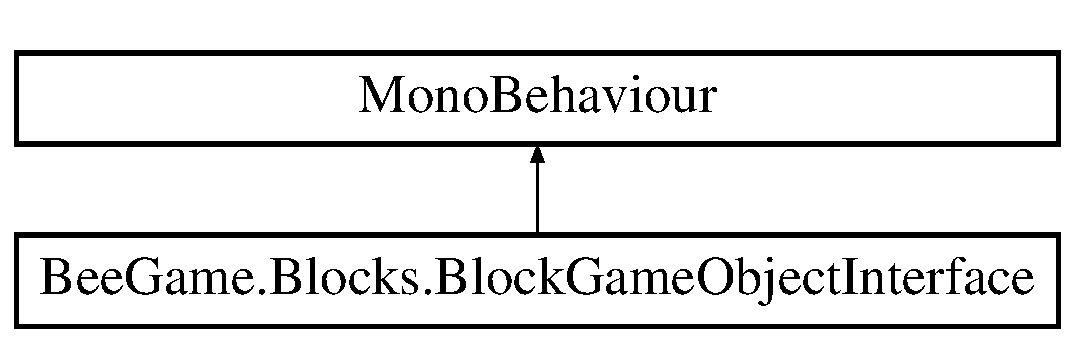
\includegraphics[height=2.000000cm]{class_bee_game_1_1_blocks_1_1_block_game_object_interface}
\end{center}
\end{figure}
\subsection*{Public Member Functions}
\begin{DoxyCompactItemize}
\item 
void \hyperlink{class_bee_game_1_1_blocks_1_1_block_game_object_interface_a3ddd5f34156385516a9ad3572160fd99}{Update\+Block\+Data} (\hyperlink{struct_bee_game_1_1_items_1_1_item}{Item} item, \hyperlink{struct_bee_game_1_1_t_h_vector3}{T\+H\+Vector3} \+\_\+position)
\begin{DoxyCompactList}\small\item\em Updates the \hyperlink{class_bee_game_1_1_blocks_1_1_block}{Block} that this Game\+Object is reprsenting \end{DoxyCompactList}\item 
void \hyperlink{class_bee_game_1_1_blocks_1_1_block_game_object_interface_ad3f4f53d3fdb09f46f05a23faa08c12a}{Update\+Block\+Data} (\hyperlink{class_bee_game_1_1_blocks_1_1_block}{Block} block\+Data)
\begin{DoxyCompactList}\small\item\em Overload that can be used if \hyperlink{class_bee_game_1_1_blocks_1_1_block}{Block} possibly contains items eg a chest \end{DoxyCompactList}\item 
\hyperlink{class_bee_game_1_1_blocks_1_1_block}{Block} \hyperlink{class_bee_game_1_1_blocks_1_1_block_game_object_interface_a40b044d5bf2a857ea25796685e23f768}{Return\+Block\+Data} ()
\begin{DoxyCompactList}\small\item\em Returns the block\textquotesingle{}s block data \end{DoxyCompactList}\item 
\hyperlink{struct_bee_game_1_1_items_1_1_item}{Item} \hyperlink{class_bee_game_1_1_blocks_1_1_block_game_object_interface_a224ae292be961a0c3b7675e5a85ddb1b}{Return\+Item\+Data} ()
\begin{DoxyCompactList}\small\item\em Returns the blocks item data \end{DoxyCompactList}\item 
Game\+Object \hyperlink{class_bee_game_1_1_blocks_1_1_block_game_object_interface_acc64daab8f2771a344aa386fa4b86c3b}{Get\+Block\+Gameobject} ()
\begin{DoxyCompactList}\small\item\em Returns the blocks Game\+Object \end{DoxyCompactList}\item 
void \hyperlink{class_bee_game_1_1_blocks_1_1_block_game_object_interface_a2e81344ecd9ed4dc9ce8b4a93b119ca2}{Update\+Chest\+Data} (\hyperlink{struct_bee_game_1_1_items_1_1_item}{Item}\mbox{[}$\,$\mbox{]} items)
\begin{DoxyCompactList}\small\item\em updates the chest inventory data \end{DoxyCompactList}\item 
\hyperlink{struct_bee_game_1_1_items_1_1_item}{Item} \mbox{[}$\,$\mbox{]} \hyperlink{class_bee_game_1_1_blocks_1_1_block_game_object_interface_a9e53e6213fec0b1f7a3ed16f50e3d894}{Apply\+Item\+Array} ()
\begin{DoxyCompactList}\small\item\em Returns the items currently in the chests inventory \end{DoxyCompactList}\item 
void \hyperlink{class_bee_game_1_1_blocks_1_1_block_game_object_interface_acecdd76ab9fd7639409fe29ebd29d4fd}{Update\+Item\+Array} (\hyperlink{struct_bee_game_1_1_items_1_1_item}{Item}\mbox{[}$\,$\mbox{]} items)
\begin{DoxyCompactList}\small\item\em updates \hyperlink{class_bee_game_1_1_blocks_1_1_block_a54846c7c7ec2f512484b3060de977fac}{Block.\+inventory\+Items} \end{DoxyCompactList}\end{DoxyCompactItemize}
\subsection*{Public Attributes}
\begin{DoxyCompactItemize}
\item 
\hyperlink{class_bee_game_1_1_blocks_1_1_block}{Block} \hyperlink{class_bee_game_1_1_blocks_1_1_block_game_object_interface_a238bad3b956ec84c8b1cc3127948b75d}{block}
\begin{DoxyCompactList}\small\item\em This blocks block data \end{DoxyCompactList}\end{DoxyCompactItemize}


\subsection{Detailed Description}
Interface between Game\+Object and \hyperlink{class_bee_game_1_1_blocks_1_1_block}{Block} data as Mono\+Behaviour dreived classes are Non-\/\+Serializable using c\# Binary\+Formatter 



Definition at line 11 of file Block\+Game\+Object\+Interface.\+cs.



\subsection{Member Function Documentation}
\mbox{\Hypertarget{class_bee_game_1_1_blocks_1_1_block_game_object_interface_a9e53e6213fec0b1f7a3ed16f50e3d894}\label{class_bee_game_1_1_blocks_1_1_block_game_object_interface_a9e53e6213fec0b1f7a3ed16f50e3d894}} 
\index{Bee\+Game\+::\+Blocks\+::\+Block\+Game\+Object\+Interface@{Bee\+Game\+::\+Blocks\+::\+Block\+Game\+Object\+Interface}!Apply\+Item\+Array@{Apply\+Item\+Array}}
\index{Apply\+Item\+Array@{Apply\+Item\+Array}!Bee\+Game\+::\+Blocks\+::\+Block\+Game\+Object\+Interface@{Bee\+Game\+::\+Blocks\+::\+Block\+Game\+Object\+Interface}}
\subsubsection{\texorpdfstring{Apply\+Item\+Array()}{ApplyItemArray()}}
{\footnotesize\ttfamily \hyperlink{struct_bee_game_1_1_items_1_1_item}{Item} \mbox{[}$\,$\mbox{]} Bee\+Game.\+Blocks.\+Block\+Game\+Object\+Interface.\+Apply\+Item\+Array (\begin{DoxyParamCaption}{ }\end{DoxyParamCaption})}



Returns the items currently in the chests inventory 

\begin{DoxyReturn}{Returns}
Item\mbox{[}$\,$\mbox{]}
\end{DoxyReturn}


Definition at line 86 of file Block\+Game\+Object\+Interface.\+cs.


\begin{DoxyCode}
87         \{
88             \textcolor{keywordflow}{return} \hyperlink{class_bee_game_1_1_blocks_1_1_block_game_object_interface_a238bad3b956ec84c8b1cc3127948b75d}{block}.\hyperlink{class_bee_game_1_1_blocks_1_1_block_a54846c7c7ec2f512484b3060de977fac}{inventoryItems};
89         \}
\end{DoxyCode}
\mbox{\Hypertarget{class_bee_game_1_1_blocks_1_1_block_game_object_interface_acc64daab8f2771a344aa386fa4b86c3b}\label{class_bee_game_1_1_blocks_1_1_block_game_object_interface_acc64daab8f2771a344aa386fa4b86c3b}} 
\index{Bee\+Game\+::\+Blocks\+::\+Block\+Game\+Object\+Interface@{Bee\+Game\+::\+Blocks\+::\+Block\+Game\+Object\+Interface}!Get\+Block\+Gameobject@{Get\+Block\+Gameobject}}
\index{Get\+Block\+Gameobject@{Get\+Block\+Gameobject}!Bee\+Game\+::\+Blocks\+::\+Block\+Game\+Object\+Interface@{Bee\+Game\+::\+Blocks\+::\+Block\+Game\+Object\+Interface}}
\subsubsection{\texorpdfstring{Get\+Block\+Gameobject()}{GetBlockGameobject()}}
{\footnotesize\ttfamily Game\+Object Bee\+Game.\+Blocks.\+Block\+Game\+Object\+Interface.\+Get\+Block\+Gameobject (\begin{DoxyParamCaption}{ }\end{DoxyParamCaption})}



Returns the blocks Game\+Object 

\begin{DoxyReturn}{Returns}
Game\+Object
\end{DoxyReturn}


Definition at line 64 of file Block\+Game\+Object\+Interface.\+cs.


\begin{DoxyCode}
65         \{
66             \hyperlink{class_bee_game_1_1_blocks_1_1_block_game_object_interface_a238bad3b956ec84c8b1cc3127948b75d}{block}.\hyperlink{class_bee_game_1_1_blocks_1_1_block_addc8d61c8acab21b0f15df5fed804f11}{item}.\hyperlink{struct_bee_game_1_1_items_1_1_item_a29abdb5010a23262e7562720bb85c171}{UpdateSpriteAndObject}();
67             \textcolor{keywordflow}{return} \hyperlink{class_bee_game_1_1_blocks_1_1_block_game_object_interface_a238bad3b956ec84c8b1cc3127948b75d}{block}.\hyperlink{class_bee_game_1_1_blocks_1_1_block_addc8d61c8acab21b0f15df5fed804f11}{item}.\hyperlink{struct_bee_game_1_1_items_1_1_item_af28a8cd4a0eff9d4c18189c5ab525f18}{itemGameobject};
68         \}
\end{DoxyCode}
\mbox{\Hypertarget{class_bee_game_1_1_blocks_1_1_block_game_object_interface_a40b044d5bf2a857ea25796685e23f768}\label{class_bee_game_1_1_blocks_1_1_block_game_object_interface_a40b044d5bf2a857ea25796685e23f768}} 
\index{Bee\+Game\+::\+Blocks\+::\+Block\+Game\+Object\+Interface@{Bee\+Game\+::\+Blocks\+::\+Block\+Game\+Object\+Interface}!Return\+Block\+Data@{Return\+Block\+Data}}
\index{Return\+Block\+Data@{Return\+Block\+Data}!Bee\+Game\+::\+Blocks\+::\+Block\+Game\+Object\+Interface@{Bee\+Game\+::\+Blocks\+::\+Block\+Game\+Object\+Interface}}
\subsubsection{\texorpdfstring{Return\+Block\+Data()}{ReturnBlockData()}}
{\footnotesize\ttfamily \hyperlink{class_bee_game_1_1_blocks_1_1_block}{Block} Bee\+Game.\+Blocks.\+Block\+Game\+Object\+Interface.\+Return\+Block\+Data (\begin{DoxyParamCaption}{ }\end{DoxyParamCaption})}



Returns the block\textquotesingle{}s block data 

\begin{DoxyReturn}{Returns}
\hyperlink{class_bee_game_1_1_blocks_1_1_block}{Block}
\end{DoxyReturn}


Definition at line 46 of file Block\+Game\+Object\+Interface.\+cs.


\begin{DoxyCode}
47         \{
48             \textcolor{keywordflow}{return} \hyperlink{class_bee_game_1_1_blocks_1_1_block_game_object_interface_a238bad3b956ec84c8b1cc3127948b75d}{block};
49         \}
\end{DoxyCode}
\mbox{\Hypertarget{class_bee_game_1_1_blocks_1_1_block_game_object_interface_a224ae292be961a0c3b7675e5a85ddb1b}\label{class_bee_game_1_1_blocks_1_1_block_game_object_interface_a224ae292be961a0c3b7675e5a85ddb1b}} 
\index{Bee\+Game\+::\+Blocks\+::\+Block\+Game\+Object\+Interface@{Bee\+Game\+::\+Blocks\+::\+Block\+Game\+Object\+Interface}!Return\+Item\+Data@{Return\+Item\+Data}}
\index{Return\+Item\+Data@{Return\+Item\+Data}!Bee\+Game\+::\+Blocks\+::\+Block\+Game\+Object\+Interface@{Bee\+Game\+::\+Blocks\+::\+Block\+Game\+Object\+Interface}}
\subsubsection{\texorpdfstring{Return\+Item\+Data()}{ReturnItemData()}}
{\footnotesize\ttfamily \hyperlink{struct_bee_game_1_1_items_1_1_item}{Item} Bee\+Game.\+Blocks.\+Block\+Game\+Object\+Interface.\+Return\+Item\+Data (\begin{DoxyParamCaption}{ }\end{DoxyParamCaption})}



Returns the blocks item data 

\begin{DoxyReturn}{Returns}
\hyperlink{class_bee_game_1_1_blocks_1_1_block_addc8d61c8acab21b0f15df5fed804f11}{Block.\+item}
\end{DoxyReturn}


Definition at line 55 of file Block\+Game\+Object\+Interface.\+cs.


\begin{DoxyCode}
56         \{
57             \textcolor{keywordflow}{return} \hyperlink{class_bee_game_1_1_blocks_1_1_block_game_object_interface_a238bad3b956ec84c8b1cc3127948b75d}{block}.\hyperlink{class_bee_game_1_1_blocks_1_1_block_addc8d61c8acab21b0f15df5fed804f11}{item};
58         \}
\end{DoxyCode}
\mbox{\Hypertarget{class_bee_game_1_1_blocks_1_1_block_game_object_interface_a3ddd5f34156385516a9ad3572160fd99}\label{class_bee_game_1_1_blocks_1_1_block_game_object_interface_a3ddd5f34156385516a9ad3572160fd99}} 
\index{Bee\+Game\+::\+Blocks\+::\+Block\+Game\+Object\+Interface@{Bee\+Game\+::\+Blocks\+::\+Block\+Game\+Object\+Interface}!Update\+Block\+Data@{Update\+Block\+Data}}
\index{Update\+Block\+Data@{Update\+Block\+Data}!Bee\+Game\+::\+Blocks\+::\+Block\+Game\+Object\+Interface@{Bee\+Game\+::\+Blocks\+::\+Block\+Game\+Object\+Interface}}
\subsubsection{\texorpdfstring{Update\+Block\+Data()}{UpdateBlockData()}\hspace{0.1cm}{\footnotesize\ttfamily [1/2]}}
{\footnotesize\ttfamily void Bee\+Game.\+Blocks.\+Block\+Game\+Object\+Interface.\+Update\+Block\+Data (\begin{DoxyParamCaption}\item[{\hyperlink{struct_bee_game_1_1_items_1_1_item}{Item}}]{item,  }\item[{\hyperlink{struct_bee_game_1_1_t_h_vector3}{T\+H\+Vector3}}]{\+\_\+position }\end{DoxyParamCaption})}



Updates the \hyperlink{class_bee_game_1_1_blocks_1_1_block}{Block} that this Game\+Object is reprsenting 


\begin{DoxyParams}{Parameters}
{\em item} & Item this this block is\\
\hline
{\em \+\_\+position} & positon of the block\\
\hline
\end{DoxyParams}


Definition at line 24 of file Block\+Game\+Object\+Interface.\+cs.


\begin{DoxyCode}
25         \{
26             \hyperlink{class_bee_game_1_1_blocks_1_1_block_game_object_interface_a238bad3b956ec84c8b1cc3127948b75d}{block} = \textcolor{keyword}{new} Block();
27             \hyperlink{class_bee_game_1_1_blocks_1_1_block_game_object_interface_a238bad3b956ec84c8b1cc3127948b75d}{block}.\hyperlink{class_bee_game_1_1_blocks_1_1_block_addc8d61c8acab21b0f15df5fed804f11}{item} = item;
28             \hyperlink{class_bee_game_1_1_blocks_1_1_block_game_object_interface_a238bad3b956ec84c8b1cc3127948b75d}{block}.\hyperlink{class_bee_game_1_1_blocks_1_1_block_a4bdeec76cfc1291eab6cebcd569620e6}{position} = \_position;
29             \hyperlink{class_bee_game_1_1_blocks_1_1_block_game_object_interface_a238bad3b956ec84c8b1cc3127948b75d}{block}.\hyperlink{class_bee_game_1_1_blocks_1_1_block_addc8d61c8acab21b0f15df5fed804f11}{item}.\hyperlink{struct_bee_game_1_1_items_1_1_item_aaa169917b0e0f8472f20398d5d448388}{stackCount} = 1;
30         \}
\end{DoxyCode}
\mbox{\Hypertarget{class_bee_game_1_1_blocks_1_1_block_game_object_interface_ad3f4f53d3fdb09f46f05a23faa08c12a}\label{class_bee_game_1_1_blocks_1_1_block_game_object_interface_ad3f4f53d3fdb09f46f05a23faa08c12a}} 
\index{Bee\+Game\+::\+Blocks\+::\+Block\+Game\+Object\+Interface@{Bee\+Game\+::\+Blocks\+::\+Block\+Game\+Object\+Interface}!Update\+Block\+Data@{Update\+Block\+Data}}
\index{Update\+Block\+Data@{Update\+Block\+Data}!Bee\+Game\+::\+Blocks\+::\+Block\+Game\+Object\+Interface@{Bee\+Game\+::\+Blocks\+::\+Block\+Game\+Object\+Interface}}
\subsubsection{\texorpdfstring{Update\+Block\+Data()}{UpdateBlockData()}\hspace{0.1cm}{\footnotesize\ttfamily [2/2]}}
{\footnotesize\ttfamily void Bee\+Game.\+Blocks.\+Block\+Game\+Object\+Interface.\+Update\+Block\+Data (\begin{DoxyParamCaption}\item[{\hyperlink{class_bee_game_1_1_blocks_1_1_block}{Block}}]{block\+Data }\end{DoxyParamCaption})}



Overload that can be used if \hyperlink{class_bee_game_1_1_blocks_1_1_block}{Block} possibly contains items eg a chest 


\begin{DoxyParams}{Parameters}
{\em block\+Data} & \hyperlink{namespace_bee_game_1_1_blocks}{Blocks} data\\
\hline
\end{DoxyParams}


Definition at line 36 of file Block\+Game\+Object\+Interface.\+cs.


\begin{DoxyCode}
37         \{
38             \hyperlink{class_bee_game_1_1_blocks_1_1_block_game_object_interface_a238bad3b956ec84c8b1cc3127948b75d}{block} = blockData;
39             \hyperlink{class_bee_game_1_1_blocks_1_1_block_game_object_interface_a238bad3b956ec84c8b1cc3127948b75d}{block}.\hyperlink{class_bee_game_1_1_blocks_1_1_block_addc8d61c8acab21b0f15df5fed804f11}{item}.\hyperlink{struct_bee_game_1_1_items_1_1_item_aaa169917b0e0f8472f20398d5d448388}{stackCount} = 1;
40         \}
\end{DoxyCode}
\mbox{\Hypertarget{class_bee_game_1_1_blocks_1_1_block_game_object_interface_a2e81344ecd9ed4dc9ce8b4a93b119ca2}\label{class_bee_game_1_1_blocks_1_1_block_game_object_interface_a2e81344ecd9ed4dc9ce8b4a93b119ca2}} 
\index{Bee\+Game\+::\+Blocks\+::\+Block\+Game\+Object\+Interface@{Bee\+Game\+::\+Blocks\+::\+Block\+Game\+Object\+Interface}!Update\+Chest\+Data@{Update\+Chest\+Data}}
\index{Update\+Chest\+Data@{Update\+Chest\+Data}!Bee\+Game\+::\+Blocks\+::\+Block\+Game\+Object\+Interface@{Bee\+Game\+::\+Blocks\+::\+Block\+Game\+Object\+Interface}}
\subsubsection{\texorpdfstring{Update\+Chest\+Data()}{UpdateChestData()}}
{\footnotesize\ttfamily void Bee\+Game.\+Blocks.\+Block\+Game\+Object\+Interface.\+Update\+Chest\+Data (\begin{DoxyParamCaption}\item[{\hyperlink{struct_bee_game_1_1_items_1_1_item}{Item} \mbox{[}$\,$\mbox{]}}]{items }\end{DoxyParamCaption})}



updates the chest inventory data 


\begin{DoxyParams}{Parameters}
{\em items} & Item\\
\hline
\end{DoxyParams}


Definition at line 76 of file Block\+Game\+Object\+Interface.\+cs.


\begin{DoxyCode}
77         \{
78             \hyperlink{class_bee_game_1_1_blocks_1_1_block_game_object_interface_a238bad3b956ec84c8b1cc3127948b75d}{block}.\hyperlink{class_bee_game_1_1_blocks_1_1_block_a54846c7c7ec2f512484b3060de977fac}{inventoryItems} = \textcolor{keyword}{new} \hyperlink{struct_bee_game_1_1_items_1_1_item}{Item}[items.Length];
79             \hyperlink{class_bee_game_1_1_blocks_1_1_block_game_object_interface_a238bad3b956ec84c8b1cc3127948b75d}{block}.\hyperlink{class_bee_game_1_1_blocks_1_1_block_a54846c7c7ec2f512484b3060de977fac}{inventoryItems} = items;
80         \}
\end{DoxyCode}
\mbox{\Hypertarget{class_bee_game_1_1_blocks_1_1_block_game_object_interface_acecdd76ab9fd7639409fe29ebd29d4fd}\label{class_bee_game_1_1_blocks_1_1_block_game_object_interface_acecdd76ab9fd7639409fe29ebd29d4fd}} 
\index{Bee\+Game\+::\+Blocks\+::\+Block\+Game\+Object\+Interface@{Bee\+Game\+::\+Blocks\+::\+Block\+Game\+Object\+Interface}!Update\+Item\+Array@{Update\+Item\+Array}}
\index{Update\+Item\+Array@{Update\+Item\+Array}!Bee\+Game\+::\+Blocks\+::\+Block\+Game\+Object\+Interface@{Bee\+Game\+::\+Blocks\+::\+Block\+Game\+Object\+Interface}}
\subsubsection{\texorpdfstring{Update\+Item\+Array()}{UpdateItemArray()}}
{\footnotesize\ttfamily void Bee\+Game.\+Blocks.\+Block\+Game\+Object\+Interface.\+Update\+Item\+Array (\begin{DoxyParamCaption}\item[{\hyperlink{struct_bee_game_1_1_items_1_1_item}{Item} \mbox{[}$\,$\mbox{]}}]{items }\end{DoxyParamCaption})}



updates \hyperlink{class_bee_game_1_1_blocks_1_1_block_a54846c7c7ec2f512484b3060de977fac}{Block.\+inventory\+Items} 


\begin{DoxyParams}{Parameters}
{\em items} & Item\mbox{[}$\,$\mbox{]}\\
\hline
\end{DoxyParams}


Definition at line 95 of file Block\+Game\+Object\+Interface.\+cs.


\begin{DoxyCode}
96         \{
97             \textcolor{keywordflow}{if} (items != null)
98             \{
99                 \hyperlink{class_bee_game_1_1_blocks_1_1_block_game_object_interface_a238bad3b956ec84c8b1cc3127948b75d}{block}.\hyperlink{class_bee_game_1_1_blocks_1_1_block_a54846c7c7ec2f512484b3060de977fac}{inventoryItems} = \textcolor{keyword}{new} \hyperlink{struct_bee_game_1_1_items_1_1_item}{Item}[items.Length];
100                 \hyperlink{class_bee_game_1_1_blocks_1_1_block_game_object_interface_a238bad3b956ec84c8b1cc3127948b75d}{block}.\hyperlink{class_bee_game_1_1_blocks_1_1_block_a54846c7c7ec2f512484b3060de977fac}{inventoryItems} = items;
101             \}
102         \}
\end{DoxyCode}


\subsection{Member Data Documentation}
\mbox{\Hypertarget{class_bee_game_1_1_blocks_1_1_block_game_object_interface_a238bad3b956ec84c8b1cc3127948b75d}\label{class_bee_game_1_1_blocks_1_1_block_game_object_interface_a238bad3b956ec84c8b1cc3127948b75d}} 
\index{Bee\+Game\+::\+Blocks\+::\+Block\+Game\+Object\+Interface@{Bee\+Game\+::\+Blocks\+::\+Block\+Game\+Object\+Interface}!block@{block}}
\index{block@{block}!Bee\+Game\+::\+Blocks\+::\+Block\+Game\+Object\+Interface@{Bee\+Game\+::\+Blocks\+::\+Block\+Game\+Object\+Interface}}
\subsubsection{\texorpdfstring{block}{block}}
{\footnotesize\ttfamily \hyperlink{class_bee_game_1_1_blocks_1_1_block}{Block} Bee\+Game.\+Blocks.\+Block\+Game\+Object\+Interface.\+block}



This blocks block data 



Definition at line 17 of file Block\+Game\+Object\+Interface.\+cs.



The documentation for this class was generated from the following file\+:\begin{DoxyCompactItemize}
\item 
C\+:/\+Users/\+Toothless/\+Documents/\+Git\+Hub/\+Bee\+Game/\+Code/\+Bee\+Game/\+Bee\+Game/\+Blocks/\hyperlink{_block_game_object_interface_8cs}{Block\+Game\+Object\+Interface.\+cs}\end{DoxyCompactItemize}

\hypertarget{class_bee_game_1_1_inventory_1_1_chest_inventory}{}\section{Bee\+Game.\+Inventory.\+Chest\+Inventory Class Reference}
\label{class_bee_game_1_1_inventory_1_1_chest_inventory}\index{Bee\+Game.\+Inventory.\+Chest\+Inventory@{Bee\+Game.\+Inventory.\+Chest\+Inventory}}
Inheritance diagram for Bee\+Game.\+Inventory.\+Chest\+Inventory\+:\begin{figure}[H]
\begin{center}
\leavevmode
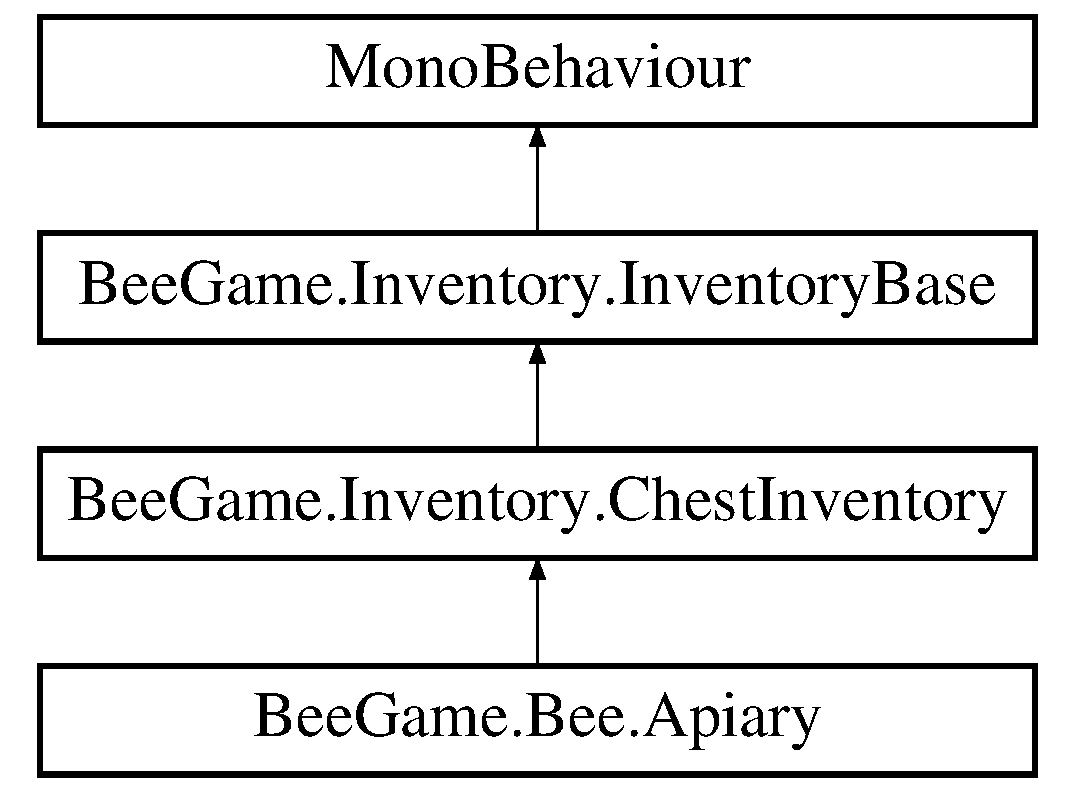
\includegraphics[height=4.000000cm]{class_bee_game_1_1_inventory_1_1_chest_inventory}
\end{center}
\end{figure}
\subsection*{Public Member Functions}
\begin{DoxyCompactItemize}
\item 
void \hyperlink{class_bee_game_1_1_inventory_1_1_chest_inventory_aecb5561a169d112e46b2270d8b8548e5}{Update\+Chest} ()
\item 
void \hyperlink{class_bee_game_1_1_inventory_1_1_chest_inventory_a9d38ab66a63c4d54bbba631e267a7149}{Chest\+Broken} ()
\item 
void \hyperlink{class_bee_game_1_1_inventory_1_1_chest_inventory_a0a42c60f89a1c79ce2be4f23da86e7b6}{Close\+Chest} ()
\begin{DoxyCompactList}\small\item\em Hides the chests invetoy and sets \hyperlink{class_bee_game_1_1_inventory_1_1_chest_inventory_a3e3529178934f2a4a8e91529c148457c}{inventory\+Open} to false \end{DoxyCompactList}\item 
void \hyperlink{class_bee_game_1_1_inventory_1_1_chest_inventory_a67be88b98076c96c0dd4450093a21c20}{Open\+Chest} (\hyperlink{class_bee_game_1_1_inventory_1_1_player_inventory}{Player\+Inventory} \+\_\+player\+Inventory)
\begin{DoxyCompactList}\small\item\em Shows the chests inventory and displayes the given players inventory within it by calling \hyperlink{class_bee_game_1_1_inventory_1_1_chest_inventory_ac08125dcf875928b702044b7a7b22a01}{Put\+Player\+Items\+In\+Chest(\+Player\+Inventory)} with the given \hyperlink{class_bee_game_1_1_inventory_1_1_player_inventory}{Player\+Inventory} sets \hyperlink{class_bee_game_1_1_inventory_1_1_chest_inventory_a3e3529178934f2a4a8e91529c148457c}{inventory\+Open} to true \end{DoxyCompactList}\end{DoxyCompactItemize}
\subsection*{Public Attributes}
\begin{DoxyCompactItemize}
\item 
Game\+Object \hyperlink{class_bee_game_1_1_inventory_1_1_chest_inventory_ac6fe8eed65557a7eb99e56d201c55466}{inventory}
\begin{DoxyCompactList}\small\item\em The chests inventory Game\+Object \end{DoxyCompactList}\end{DoxyCompactItemize}
\subsection*{Protected Attributes}
\begin{DoxyCompactItemize}
\item 
\hyperlink{class_bee_game_1_1_blocks_1_1_block_game_object_interface}{Block\+Game\+Object\+Interface} \hyperlink{class_bee_game_1_1_inventory_1_1_chest_inventory_aa18498b9af704585d4c747ff5a7444f8}{block\+Interface}
\begin{DoxyCompactList}\small\item\em The chests block interface where the items int he inventory will be stored \end{DoxyCompactList}\end{DoxyCompactItemize}
\subsection*{Private Member Functions}
\begin{DoxyCompactItemize}
\item 
void \hyperlink{class_bee_game_1_1_inventory_1_1_chest_inventory_aa1ba251e8466684dc8a16b53afadbf90}{Awake} ()
\begin{DoxyCompactList}\small\item\em When the chest is made the number of slots is calculated and the inventory is set to be inactive \end{DoxyCompactList}\item 
void \hyperlink{class_bee_game_1_1_inventory_1_1_chest_inventory_a3476b739dab6ac46a8152da085d8399a}{Start} ()
\begin{DoxyCompactList}\small\item\em Sets the \hyperlink{class_bee_game_1_1_inventory_1_1_chest_inventory_aa18498b9af704585d4c747ff5a7444f8}{block\+Interface} Makes the \hyperlink{class_bee_game_1_1_inventory_1_1_inventory_base_a405502a6eabf14e1498d96dc8aff5e8d}{Inventory\+Base.\+slotand\+Item} array \end{DoxyCompactList}\item 
void \hyperlink{class_bee_game_1_1_inventory_1_1_chest_inventory_ad2b02fa5934d7447cd236180435a4d0f}{Update} ()
\begin{DoxyCompactList}\small\item\em If the inventory os open checks if it should be closed, if it sould calls \hyperlink{class_bee_game_1_1_inventory_1_1_chest_inventory_a0a42c60f89a1c79ce2be4f23da86e7b6}{Close\+Chest}. Also Updates the chests \hyperlink{class_bee_game_1_1_inventory_1_1_inventory_base}{Inventory\+Base} by calling \hyperlink{class_bee_game_1_1_inventory_1_1_inventory_base_aa1a965cf7ba9e04b22a4ef85ad133854}{Inventory\+Base.\+Update\+Base} \end{DoxyCompactList}\item 
void \hyperlink{class_bee_game_1_1_inventory_1_1_chest_inventory_a3e9326154a7f2602ba03bd6b21aba93f}{Save\+Chest\+Items} ()
\begin{DoxyCompactList}\small\item\em Puts the chests current contence into the item\mbox{[}\mbox{]} in Block\+Game\+Object\+Interface \end{DoxyCompactList}\item 
void \hyperlink{class_bee_game_1_1_inventory_1_1_chest_inventory_a426c17adf8e95a36e24f9793f6c90b48}{Update\+Player\+Inventory} (\hyperlink{class_bee_game_1_1_inventory_1_1_player_inventory}{Player\+Inventory} \+\_\+playerinventoy)
\begin{DoxyCompactList}\small\item\em When the chest is closed this updates the player inventory to any changes eg and item has been added or removed \end{DoxyCompactList}\item 
void \hyperlink{class_bee_game_1_1_inventory_1_1_chest_inventory_ac08125dcf875928b702044b7a7b22a01}{Put\+Player\+Items\+In\+Chest} (\hyperlink{class_bee_game_1_1_inventory_1_1_player_inventory}{Player\+Inventory} \+\_\+playerinventory)
\begin{DoxyCompactList}\small\item\em Puts the items in the players inventory in the correct slots so that they are displayed correctly in the chest \end{DoxyCompactList}\end{DoxyCompactItemize}
\subsection*{Private Attributes}
\begin{DoxyCompactItemize}
\item 
\hyperlink{class_bee_game_1_1_inventory_1_1_player_inventory}{Player\+Inventory} \hyperlink{class_bee_game_1_1_inventory_1_1_chest_inventory_a79ff450013724b84c1c21858c63404b0}{playerinventory}
\begin{DoxyCompactList}\small\item\em The players inventory \end{DoxyCompactList}\item 
bool \hyperlink{class_bee_game_1_1_inventory_1_1_chest_inventory_a3e3529178934f2a4a8e91529c148457c}{inventory\+Open}
\begin{DoxyCompactList}\small\item\em Is the inventory Open \end{DoxyCompactList}\end{DoxyCompactItemize}
\subsection*{Additional Inherited Members}


\subsection{Detailed Description}


Definition at line 8 of file Chest\+Inventory.\+cs.



\subsection{Member Function Documentation}
\mbox{\Hypertarget{class_bee_game_1_1_inventory_1_1_chest_inventory_aa1ba251e8466684dc8a16b53afadbf90}\label{class_bee_game_1_1_inventory_1_1_chest_inventory_aa1ba251e8466684dc8a16b53afadbf90}} 
\index{Bee\+Game\+::\+Inventory\+::\+Chest\+Inventory@{Bee\+Game\+::\+Inventory\+::\+Chest\+Inventory}!Awake@{Awake}}
\index{Awake@{Awake}!Bee\+Game\+::\+Inventory\+::\+Chest\+Inventory@{Bee\+Game\+::\+Inventory\+::\+Chest\+Inventory}}
\subsubsection{\texorpdfstring{Awake()}{Awake()}}
{\footnotesize\ttfamily void Bee\+Game.\+Inventory.\+Chest\+Inventory.\+Awake (\begin{DoxyParamCaption}{ }\end{DoxyParamCaption})\hspace{0.3cm}{\ttfamily [private]}}



When the chest is made the number of slots is calculated and the inventory is set to be inactive 



Definition at line 38 of file Chest\+Inventory.\+cs.


\begin{DoxyCode}
39         \{
40             \textcolor{comment}{//slots = (uint)inventoryGUI.Length - 25;}
41             \hyperlink{class_bee_game_1_1_inventory_1_1_chest_inventory_ac6fe8eed65557a7eb99e56d201c55466}{inventory}.SetActive(\textcolor{keyword}{false});
42         \}
\end{DoxyCode}
\mbox{\Hypertarget{class_bee_game_1_1_inventory_1_1_chest_inventory_a9d38ab66a63c4d54bbba631e267a7149}\label{class_bee_game_1_1_inventory_1_1_chest_inventory_a9d38ab66a63c4d54bbba631e267a7149}} 
\index{Bee\+Game\+::\+Inventory\+::\+Chest\+Inventory@{Bee\+Game\+::\+Inventory\+::\+Chest\+Inventory}!Chest\+Broken@{Chest\+Broken}}
\index{Chest\+Broken@{Chest\+Broken}!Bee\+Game\+::\+Inventory\+::\+Chest\+Inventory@{Bee\+Game\+::\+Inventory\+::\+Chest\+Inventory}}
\subsubsection{\texorpdfstring{Chest\+Broken()}{ChestBroken()}}
{\footnotesize\ttfamily void Bee\+Game.\+Inventory.\+Chest\+Inventory.\+Chest\+Broken (\begin{DoxyParamCaption}{ }\end{DoxyParamCaption})}





\begin{DoxyRefDesc}{Todo}
\item[\hyperlink{todo__todo000005}{Todo}]Currently this finction does nothing, must finish, should spawn items in the chests inventory when it is broken \end{DoxyRefDesc}


Definition at line 91 of file Chest\+Inventory.\+cs.


\begin{DoxyCode}
92         \{
93         \}
\end{DoxyCode}
\mbox{\Hypertarget{class_bee_game_1_1_inventory_1_1_chest_inventory_a0a42c60f89a1c79ce2be4f23da86e7b6}\label{class_bee_game_1_1_inventory_1_1_chest_inventory_a0a42c60f89a1c79ce2be4f23da86e7b6}} 
\index{Bee\+Game\+::\+Inventory\+::\+Chest\+Inventory@{Bee\+Game\+::\+Inventory\+::\+Chest\+Inventory}!Close\+Chest@{Close\+Chest}}
\index{Close\+Chest@{Close\+Chest}!Bee\+Game\+::\+Inventory\+::\+Chest\+Inventory@{Bee\+Game\+::\+Inventory\+::\+Chest\+Inventory}}
\subsubsection{\texorpdfstring{Close\+Chest()}{CloseChest()}}
{\footnotesize\ttfamily void Bee\+Game.\+Inventory.\+Chest\+Inventory.\+Close\+Chest (\begin{DoxyParamCaption}{ }\end{DoxyParamCaption})}



Hides the chests invetoy and sets \hyperlink{class_bee_game_1_1_inventory_1_1_chest_inventory_a3e3529178934f2a4a8e91529c148457c}{inventory\+Open} to false 



Definition at line 106 of file Chest\+Inventory.\+cs.


\begin{DoxyCode}
107         \{
108             \hyperlink{class_bee_game_1_1_inventory_1_1_chest_inventory_ac6fe8eed65557a7eb99e56d201c55466}{inventory}.SetActive(\textcolor{keyword}{false});
109             \hyperlink{class_bee_game_1_1_inventory_1_1_chest_inventory_a79ff450013724b84c1c21858c63404b0}{playerinventory}.\hyperlink{class_bee_game_1_1_inventory_1_1_player_inventory_a595e1144315e0e9be0b825b538643e1f}{heldObjectInventory}.SetActive(\textcolor{keyword}{true});
110             \hyperlink{class_bee_game_1_1_inventory_1_1_chest_inventory_a426c17adf8e95a36e24f9793f6c90b48}{UpdatePlayerInventory}(\hyperlink{class_bee_game_1_1_inventory_1_1_chest_inventory_a79ff450013724b84c1c21858c63404b0}{playerinventory});
111             
112             Time.timeScale = 1;
113             Cursor.visible = \textcolor{keyword}{false};
114             Cursor.lockState = CursorLockMode.Locked;
115 
116             \hyperlink{class_bee_game_1_1_inventory_1_1_chest_inventory_a3e3529178934f2a4a8e91529c148457c}{inventoryOpen} = \textcolor{keyword}{false};
117         \}
\end{DoxyCode}
\mbox{\Hypertarget{class_bee_game_1_1_inventory_1_1_chest_inventory_a67be88b98076c96c0dd4450093a21c20}\label{class_bee_game_1_1_inventory_1_1_chest_inventory_a67be88b98076c96c0dd4450093a21c20}} 
\index{Bee\+Game\+::\+Inventory\+::\+Chest\+Inventory@{Bee\+Game\+::\+Inventory\+::\+Chest\+Inventory}!Open\+Chest@{Open\+Chest}}
\index{Open\+Chest@{Open\+Chest}!Bee\+Game\+::\+Inventory\+::\+Chest\+Inventory@{Bee\+Game\+::\+Inventory\+::\+Chest\+Inventory}}
\subsubsection{\texorpdfstring{Open\+Chest()}{OpenChest()}}
{\footnotesize\ttfamily void Bee\+Game.\+Inventory.\+Chest\+Inventory.\+Open\+Chest (\begin{DoxyParamCaption}\item[{\hyperlink{class_bee_game_1_1_inventory_1_1_player_inventory}{Player\+Inventory}}]{\+\_\+player\+Inventory }\end{DoxyParamCaption})}



Shows the chests inventory and displayes the given players inventory within it by calling \hyperlink{class_bee_game_1_1_inventory_1_1_chest_inventory_ac08125dcf875928b702044b7a7b22a01}{Put\+Player\+Items\+In\+Chest(\+Player\+Inventory)} with the given \hyperlink{class_bee_game_1_1_inventory_1_1_player_inventory}{Player\+Inventory} sets \hyperlink{class_bee_game_1_1_inventory_1_1_chest_inventory_a3e3529178934f2a4a8e91529c148457c}{inventory\+Open} to true 


\begin{DoxyParams}{Parameters}
{\em \+\_\+player\+Inventory} & \hyperlink{class_bee_game_1_1_inventory_1_1_player_inventory}{Player\+Inventory}\\
\hline
\end{DoxyParams}


Definition at line 124 of file Chest\+Inventory.\+cs.


\begin{DoxyCode}
125         \{
126             \_playerInventory.heldObjectInventory.SetActive(\textcolor{keyword}{false});
127             \hyperlink{class_bee_game_1_1_inventory_1_1_chest_inventory_ac08125dcf875928b702044b7a7b22a01}{PutPlayerItemsInChest}(\_playerInventory);
128 
129             Time.timeScale = 0;
130             Cursor.visible = \textcolor{keyword}{true};
131             Cursor.lockState = CursorLockMode.None;
132 
133             \hyperlink{class_bee_game_1_1_inventory_1_1_chest_inventory_ac6fe8eed65557a7eb99e56d201c55466}{inventory}.SetActive(\textcolor{keyword}{true});
134 
135             \hyperlink{class_bee_game_1_1_inventory_1_1_chest_inventory_a3e3529178934f2a4a8e91529c148457c}{inventoryOpen} = \textcolor{keyword}{true};
136         \}
\end{DoxyCode}
\mbox{\Hypertarget{class_bee_game_1_1_inventory_1_1_chest_inventory_ac08125dcf875928b702044b7a7b22a01}\label{class_bee_game_1_1_inventory_1_1_chest_inventory_ac08125dcf875928b702044b7a7b22a01}} 
\index{Bee\+Game\+::\+Inventory\+::\+Chest\+Inventory@{Bee\+Game\+::\+Inventory\+::\+Chest\+Inventory}!Put\+Player\+Items\+In\+Chest@{Put\+Player\+Items\+In\+Chest}}
\index{Put\+Player\+Items\+In\+Chest@{Put\+Player\+Items\+In\+Chest}!Bee\+Game\+::\+Inventory\+::\+Chest\+Inventory@{Bee\+Game\+::\+Inventory\+::\+Chest\+Inventory}}
\subsubsection{\texorpdfstring{Put\+Player\+Items\+In\+Chest()}{PutPlayerItemsInChest()}}
{\footnotesize\ttfamily void Bee\+Game.\+Inventory.\+Chest\+Inventory.\+Put\+Player\+Items\+In\+Chest (\begin{DoxyParamCaption}\item[{\hyperlink{class_bee_game_1_1_inventory_1_1_player_inventory}{Player\+Inventory}}]{\+\_\+playerinventory }\end{DoxyParamCaption})\hspace{0.3cm}{\ttfamily [private]}}



Puts the items in the players inventory in the correct slots so that they are displayed correctly in the chest 


\begin{DoxyParams}{Parameters}
{\em \+\_\+playerinventory} & \hyperlink{class_bee_game_1_1_inventory_1_1_player_inventory}{Player\+Inventory}\\
\hline
\end{DoxyParams}


Definition at line 156 of file Chest\+Inventory.\+cs.


\begin{DoxyCode}
157         \{
158             \textcolor{keywordflow}{for}(\textcolor{keywordtype}{int} i = 0; i < \_playerinventory.slotandItem.Length; i++)
159             \{
160                 \hyperlink{class_bee_game_1_1_inventory_1_1_inventory_base_a405502a6eabf14e1498d96dc8aff5e8d}{slotandItem}[i] = \_playerinventory.slotandItem[i];
161             \}
162 
163             \hyperlink{class_bee_game_1_1_inventory_1_1_chest_inventory_a79ff450013724b84c1c21858c63404b0}{playerinventory} = \_playerinventory;
164             \hyperlink{class_bee_game_1_1_inventory_1_1_inventory_base_ac8edbffe8b164d66297c127654c844c4}{UpdateSlots}();
165         \}
\end{DoxyCode}
\mbox{\Hypertarget{class_bee_game_1_1_inventory_1_1_chest_inventory_a3e9326154a7f2602ba03bd6b21aba93f}\label{class_bee_game_1_1_inventory_1_1_chest_inventory_a3e9326154a7f2602ba03bd6b21aba93f}} 
\index{Bee\+Game\+::\+Inventory\+::\+Chest\+Inventory@{Bee\+Game\+::\+Inventory\+::\+Chest\+Inventory}!Save\+Chest\+Items@{Save\+Chest\+Items}}
\index{Save\+Chest\+Items@{Save\+Chest\+Items}!Bee\+Game\+::\+Inventory\+::\+Chest\+Inventory@{Bee\+Game\+::\+Inventory\+::\+Chest\+Inventory}}
\subsubsection{\texorpdfstring{Save\+Chest\+Items()}{SaveChestItems()}}
{\footnotesize\ttfamily void Bee\+Game.\+Inventory.\+Chest\+Inventory.\+Save\+Chest\+Items (\begin{DoxyParamCaption}{ }\end{DoxyParamCaption})\hspace{0.3cm}{\ttfamily [private]}}



Puts the chests current contence into the item\mbox{[}\mbox{]} in Block\+Game\+Object\+Interface 



Definition at line 98 of file Chest\+Inventory.\+cs.


\begin{DoxyCode}
99         \{
100             \hyperlink{class_bee_game_1_1_inventory_1_1_chest_inventory_aa18498b9af704585d4c747ff5a7444f8}{blockInterface}.\hyperlink{class_bee_game_1_1_blocks_1_1_block_game_object_interface_acecdd76ab9fd7639409fe29ebd29d4fd}{UpdateItemArray}(
      \hyperlink{class_bee_game_1_1_inventory_1_1_inventory_base_a405502a6eabf14e1498d96dc8aff5e8d}{slotandItem});
101         \}
\end{DoxyCode}
\mbox{\Hypertarget{class_bee_game_1_1_inventory_1_1_chest_inventory_a3476b739dab6ac46a8152da085d8399a}\label{class_bee_game_1_1_inventory_1_1_chest_inventory_a3476b739dab6ac46a8152da085d8399a}} 
\index{Bee\+Game\+::\+Inventory\+::\+Chest\+Inventory@{Bee\+Game\+::\+Inventory\+::\+Chest\+Inventory}!Start@{Start}}
\index{Start@{Start}!Bee\+Game\+::\+Inventory\+::\+Chest\+Inventory@{Bee\+Game\+::\+Inventory\+::\+Chest\+Inventory}}
\subsubsection{\texorpdfstring{Start()}{Start()}}
{\footnotesize\ttfamily void Bee\+Game.\+Inventory.\+Chest\+Inventory.\+Start (\begin{DoxyParamCaption}{ }\end{DoxyParamCaption})\hspace{0.3cm}{\ttfamily [private]}}



Sets the \hyperlink{class_bee_game_1_1_inventory_1_1_chest_inventory_aa18498b9af704585d4c747ff5a7444f8}{block\+Interface} Makes the \hyperlink{class_bee_game_1_1_inventory_1_1_inventory_base_a405502a6eabf14e1498d96dc8aff5e8d}{Inventory\+Base.\+slotand\+Item} array 



Definition at line 48 of file Chest\+Inventory.\+cs.


\begin{DoxyCode}
49         \{
50             \hyperlink{class_bee_game_1_1_inventory_1_1_chest_inventory_aa18498b9af704585d4c747ff5a7444f8}{blockInterface} = GetComponent<BlockGameObjectInterface>();
51             \hyperlink{class_bee_game_1_1_inventory_1_1_inventory_base_a405502a6eabf14e1498d96dc8aff5e8d}{slotandItem} = \hyperlink{class_bee_game_1_1_inventory_1_1_chest_inventory_aa18498b9af704585d4c747ff5a7444f8}{blockInterface}.\hyperlink{class_bee_game_1_1_blocks_1_1_block_game_object_interface_a9e53e6213fec0b1f7a3ed16f50e3d894}{ApplyItemArray}();
52 
53             \textcolor{keywordflow}{if}(slotandItem == null)
54             \{
55                 slotandItem = \textcolor{keyword}{new} \hyperlink{struct_bee_game_1_1_items_1_1_item}{Item}[\hyperlink{class_bee_game_1_1_inventory_1_1_inventory_base_a48dcba7ad7bfa1bed8c9ae290fb32857}{inventoryGUI}.Length];
56             \}
57 
58             \hyperlink{class_bee_game_1_1_inventory_1_1_inventory_base_ac8edbffe8b164d66297c127654c844c4}{UpdateSlots}();
59             \hyperlink{class_bee_game_1_1_inventory_1_1_inventory_base_aa1a965cf7ba9e04b22a4ef85ad133854}{UpdateBase}();
60         \}
\end{DoxyCode}
\mbox{\Hypertarget{class_bee_game_1_1_inventory_1_1_chest_inventory_ad2b02fa5934d7447cd236180435a4d0f}\label{class_bee_game_1_1_inventory_1_1_chest_inventory_ad2b02fa5934d7447cd236180435a4d0f}} 
\index{Bee\+Game\+::\+Inventory\+::\+Chest\+Inventory@{Bee\+Game\+::\+Inventory\+::\+Chest\+Inventory}!Update@{Update}}
\index{Update@{Update}!Bee\+Game\+::\+Inventory\+::\+Chest\+Inventory@{Bee\+Game\+::\+Inventory\+::\+Chest\+Inventory}}
\subsubsection{\texorpdfstring{Update()}{Update()}}
{\footnotesize\ttfamily void Bee\+Game.\+Inventory.\+Chest\+Inventory.\+Update (\begin{DoxyParamCaption}{ }\end{DoxyParamCaption})\hspace{0.3cm}{\ttfamily [private]}}



If the inventory os open checks if it should be closed, if it sould calls \hyperlink{class_bee_game_1_1_inventory_1_1_chest_inventory_a0a42c60f89a1c79ce2be4f23da86e7b6}{Close\+Chest}. Also Updates the chests \hyperlink{class_bee_game_1_1_inventory_1_1_inventory_base}{Inventory\+Base} by calling \hyperlink{class_bee_game_1_1_inventory_1_1_inventory_base_aa1a965cf7ba9e04b22a4ef85ad133854}{Inventory\+Base.\+Update\+Base} 



Definition at line 65 of file Chest\+Inventory.\+cs.


\begin{DoxyCode}
66         \{
67             \hyperlink{class_bee_game_1_1_inventory_1_1_chest_inventory_aecb5561a169d112e46b2270d8b8548e5}{UpdateChest}();
68         \}
\end{DoxyCode}
\mbox{\Hypertarget{class_bee_game_1_1_inventory_1_1_chest_inventory_aecb5561a169d112e46b2270d8b8548e5}\label{class_bee_game_1_1_inventory_1_1_chest_inventory_aecb5561a169d112e46b2270d8b8548e5}} 
\index{Bee\+Game\+::\+Inventory\+::\+Chest\+Inventory@{Bee\+Game\+::\+Inventory\+::\+Chest\+Inventory}!Update\+Chest@{Update\+Chest}}
\index{Update\+Chest@{Update\+Chest}!Bee\+Game\+::\+Inventory\+::\+Chest\+Inventory@{Bee\+Game\+::\+Inventory\+::\+Chest\+Inventory}}
\subsubsection{\texorpdfstring{Update\+Chest()}{UpdateChest()}}
{\footnotesize\ttfamily void Bee\+Game.\+Inventory.\+Chest\+Inventory.\+Update\+Chest (\begin{DoxyParamCaption}{ }\end{DoxyParamCaption})}



Definition at line 70 of file Chest\+Inventory.\+cs.


\begin{DoxyCode}
71         \{
72             \textcolor{keywordflow}{if} (\hyperlink{class_bee_game_1_1_inventory_1_1_chest_inventory_a3e3529178934f2a4a8e91529c148457c}{inventoryOpen})
73             \{
74                 \hyperlink{class_bee_game_1_1_inventory_1_1_inventory_base_aa1a965cf7ba9e04b22a4ef85ad133854}{UpdateBase}();
75             \}
76 
77             \textcolor{keywordflow}{if} (\hyperlink{class_bee_game_1_1_core_1_1_input_manager}{InputManager}.\hyperlink{class_bee_game_1_1_core_1_1_input_manager_ac90aab89652007118b67f60e962103c5}{GetButtonDown}(\textcolor{stringliteral}{"Inventory"}))
78             \{
79                 \textcolor{keywordflow}{if} (\hyperlink{class_bee_game_1_1_inventory_1_1_chest_inventory_a3e3529178934f2a4a8e91529c148457c}{inventoryOpen})
80                 \{
81                     \hyperlink{class_bee_game_1_1_inventory_1_1_chest_inventory_a0a42c60f89a1c79ce2be4f23da86e7b6}{CloseChest}();
82                 \}
83             \}
84 
85             \hyperlink{class_bee_game_1_1_inventory_1_1_chest_inventory_a3e9326154a7f2602ba03bd6b21aba93f}{SaveChestItems}();
86         \}
\end{DoxyCode}
\mbox{\Hypertarget{class_bee_game_1_1_inventory_1_1_chest_inventory_a426c17adf8e95a36e24f9793f6c90b48}\label{class_bee_game_1_1_inventory_1_1_chest_inventory_a426c17adf8e95a36e24f9793f6c90b48}} 
\index{Bee\+Game\+::\+Inventory\+::\+Chest\+Inventory@{Bee\+Game\+::\+Inventory\+::\+Chest\+Inventory}!Update\+Player\+Inventory@{Update\+Player\+Inventory}}
\index{Update\+Player\+Inventory@{Update\+Player\+Inventory}!Bee\+Game\+::\+Inventory\+::\+Chest\+Inventory@{Bee\+Game\+::\+Inventory\+::\+Chest\+Inventory}}
\subsubsection{\texorpdfstring{Update\+Player\+Inventory()}{UpdatePlayerInventory()}}
{\footnotesize\ttfamily void Bee\+Game.\+Inventory.\+Chest\+Inventory.\+Update\+Player\+Inventory (\begin{DoxyParamCaption}\item[{\hyperlink{class_bee_game_1_1_inventory_1_1_player_inventory}{Player\+Inventory}}]{\+\_\+playerinventoy }\end{DoxyParamCaption})\hspace{0.3cm}{\ttfamily [private]}}



When the chest is closed this updates the player inventory to any changes eg and item has been added or removed 


\begin{DoxyParams}{Parameters}
{\em \+\_\+playerinventoy} & \hyperlink{class_bee_game_1_1_inventory_1_1_inventory_base_ac8edbffe8b164d66297c127654c844c4}{Player\+Inventory.\+Update\+Slots}\\
\hline
\end{DoxyParams}


Definition at line 142 of file Chest\+Inventory.\+cs.


\begin{DoxyCode}
143         \{
144             \textcolor{keywordflow}{for}(\textcolor{keywordtype}{int} i = 0; i < \_playerinventoy.slotandItem.Length; i++)
145             \{
146                 \_playerinventoy.slotandItem[i] = \hyperlink{class_bee_game_1_1_inventory_1_1_inventory_base_a405502a6eabf14e1498d96dc8aff5e8d}{slotandItem}[i];
147             \}
148 
149             \_playerinventoy.UpdateSlots();
150         \}
\end{DoxyCode}


\subsection{Member Data Documentation}
\mbox{\Hypertarget{class_bee_game_1_1_inventory_1_1_chest_inventory_aa18498b9af704585d4c747ff5a7444f8}\label{class_bee_game_1_1_inventory_1_1_chest_inventory_aa18498b9af704585d4c747ff5a7444f8}} 
\index{Bee\+Game\+::\+Inventory\+::\+Chest\+Inventory@{Bee\+Game\+::\+Inventory\+::\+Chest\+Inventory}!block\+Interface@{block\+Interface}}
\index{block\+Interface@{block\+Interface}!Bee\+Game\+::\+Inventory\+::\+Chest\+Inventory@{Bee\+Game\+::\+Inventory\+::\+Chest\+Inventory}}
\subsubsection{\texorpdfstring{block\+Interface}{blockInterface}}
{\footnotesize\ttfamily \hyperlink{class_bee_game_1_1_blocks_1_1_block_game_object_interface}{Block\+Game\+Object\+Interface} Bee\+Game.\+Inventory.\+Chest\+Inventory.\+block\+Interface\hspace{0.3cm}{\ttfamily [protected]}}



The chests block interface where the items int he inventory will be stored 



Definition at line 17 of file Chest\+Inventory.\+cs.

\mbox{\Hypertarget{class_bee_game_1_1_inventory_1_1_chest_inventory_ac6fe8eed65557a7eb99e56d201c55466}\label{class_bee_game_1_1_inventory_1_1_chest_inventory_ac6fe8eed65557a7eb99e56d201c55466}} 
\index{Bee\+Game\+::\+Inventory\+::\+Chest\+Inventory@{Bee\+Game\+::\+Inventory\+::\+Chest\+Inventory}!inventory@{inventory}}
\index{inventory@{inventory}!Bee\+Game\+::\+Inventory\+::\+Chest\+Inventory@{Bee\+Game\+::\+Inventory\+::\+Chest\+Inventory}}
\subsubsection{\texorpdfstring{inventory}{inventory}}
{\footnotesize\ttfamily Game\+Object Bee\+Game.\+Inventory.\+Chest\+Inventory.\+inventory}



The chests inventory Game\+Object 



Definition at line 13 of file Chest\+Inventory.\+cs.

\mbox{\Hypertarget{class_bee_game_1_1_inventory_1_1_chest_inventory_a3e3529178934f2a4a8e91529c148457c}\label{class_bee_game_1_1_inventory_1_1_chest_inventory_a3e3529178934f2a4a8e91529c148457c}} 
\index{Bee\+Game\+::\+Inventory\+::\+Chest\+Inventory@{Bee\+Game\+::\+Inventory\+::\+Chest\+Inventory}!inventory\+Open@{inventory\+Open}}
\index{inventory\+Open@{inventory\+Open}!Bee\+Game\+::\+Inventory\+::\+Chest\+Inventory@{Bee\+Game\+::\+Inventory\+::\+Chest\+Inventory}}
\subsubsection{\texorpdfstring{inventory\+Open}{inventoryOpen}}
{\footnotesize\ttfamily bool Bee\+Game.\+Inventory.\+Chest\+Inventory.\+inventory\+Open\hspace{0.3cm}{\ttfamily [private]}}



Is the inventory Open 



Definition at line 33 of file Chest\+Inventory.\+cs.

\mbox{\Hypertarget{class_bee_game_1_1_inventory_1_1_chest_inventory_a79ff450013724b84c1c21858c63404b0}\label{class_bee_game_1_1_inventory_1_1_chest_inventory_a79ff450013724b84c1c21858c63404b0}} 
\index{Bee\+Game\+::\+Inventory\+::\+Chest\+Inventory@{Bee\+Game\+::\+Inventory\+::\+Chest\+Inventory}!playerinventory@{playerinventory}}
\index{playerinventory@{playerinventory}!Bee\+Game\+::\+Inventory\+::\+Chest\+Inventory@{Bee\+Game\+::\+Inventory\+::\+Chest\+Inventory}}
\subsubsection{\texorpdfstring{playerinventory}{playerinventory}}
{\footnotesize\ttfamily \hyperlink{class_bee_game_1_1_inventory_1_1_player_inventory}{Player\+Inventory} Bee\+Game.\+Inventory.\+Chest\+Inventory.\+playerinventory\hspace{0.3cm}{\ttfamily [private]}}



The players inventory 



Definition at line 22 of file Chest\+Inventory.\+cs.



The documentation for this class was generated from the following file\+:\begin{DoxyCompactItemize}
\item 
C\+:/\+Users/\+Toothless/\+Documents/\+Git\+Hub/\+Bee\+Game/\+Code/\+Bee\+Game/\+Bee\+Game/\+Inventory/\hyperlink{_chest_inventory_8cs}{Chest\+Inventory.\+cs}\end{DoxyCompactItemize}

\hypertarget{struct_bee_game_1_1_bee_1_1_combining_bee_data}{}\section{Bee\+Game.\+Bee.\+Combining\+Bee\+Data Struct Reference}
\label{struct_bee_game_1_1_bee_1_1_combining_bee_data}\index{Bee\+Game.\+Bee.\+Combining\+Bee\+Data@{Bee\+Game.\+Bee.\+Combining\+Bee\+Data}}


Holds the data that the bee queen in conbining with. Exists due to a \hyperlink{struct_bee_game_1_1_bee_1_1_bee_data}{Bee\+Data} variable with in a \hyperlink{struct_bee_game_1_1_bee_1_1_bee_data}{Bee\+Data} is to deep for serialization /summary$>$  


\subsection*{Public Member Functions}
\begin{DoxyCompactItemize}
\item 
void \hyperlink{struct_bee_game_1_1_bee_1_1_combining_bee_data_abdf4646728337da76097aed9b74347ae}{To\+Combining\+Bee\+Data} (\hyperlink{struct_bee_game_1_1_bee_1_1_bee_data}{Bee\+Data} data)
\item 
\hyperlink{struct_bee_game_1_1_bee_1_1_bee_data}{Bee\+Data} \hyperlink{struct_bee_game_1_1_bee_1_1_combining_bee_data_a8f49452b4800bbc401a225e2676eeca0}{To\+Bee\+Data} ()
\begin{DoxyCompactList}\small\item\em Reconverts the \hyperlink{struct_bee_game_1_1_bee_1_1_combining_bee_data}{Combining\+Bee\+Data} back to normal \hyperlink{struct_bee_game_1_1_bee_1_1_bee_data}{Bee\+Data} \end{DoxyCompactList}\end{DoxyCompactItemize}
\subsection*{Public Attributes}
\begin{DoxyCompactItemize}
\item 
\hyperlink{namespace_bee_game_1_1_enums_aa2ead984825678d83c42d48f6382619c}{Bee\+Species} \hyperlink{struct_bee_game_1_1_bee_1_1_combining_bee_data_a7e519ea913d51073b7da7815e85a4eeb}{species}
\item 
\hyperlink{namespace_bee_game_1_1_enums_ae3853807ded2f4d99a0d4a7fb4b2bc46}{Bee\+Life\+Span} \hyperlink{struct_bee_game_1_1_bee_1_1_combining_bee_data_a2635fae2aa8e50991d7733624883e671}{s\+Lifespan}
\begin{DoxyCompactList}\small\item\em Secondary \hyperlink{namespace_bee_game_1_1_enums_ae3853807ded2f4d99a0d4a7fb4b2bc46}{Bee\+Game.\+Enums.\+Bee\+Life\+Span} of the \hyperlink{namespace_bee_game_1_1_bee}{Bee} \end{DoxyCompactList}\item 
uint \hyperlink{struct_bee_game_1_1_bee_1_1_combining_bee_data_a02566c65413bebc23e767561c17510d5}{s\+Fertility}
\begin{DoxyCompactList}\small\item\em Secondary Fertility of the \hyperlink{namespace_bee_game_1_1_bee}{Bee} \end{DoxyCompactList}\item 
\hyperlink{namespace_bee_game_1_1_enums_acf7ae32a86385a40fc0c7b55af95c6c3}{Bee\+Effect} \hyperlink{struct_bee_game_1_1_bee_1_1_combining_bee_data_a6706a04242c477e5934d779fde7e7b8e}{s\+Effect}
\begin{DoxyCompactList}\small\item\em Secondary \hyperlink{namespace_bee_game_1_1_enums_acf7ae32a86385a40fc0c7b55af95c6c3}{Bee\+Game.\+Enums.\+Bee\+Effect} of the \hyperlink{namespace_bee_game_1_1_bee}{Bee} \end{DoxyCompactList}\item 
\hyperlink{namespace_bee_game_1_1_enums_afee18200a21cc4b8e1d0cdb669930f14}{Bee\+Production\+Speed} \hyperlink{struct_bee_game_1_1_bee_1_1_combining_bee_data_a253d2a55fe2cb1a3d01492a6f961b995}{s\+Prod\+Speed}
\begin{DoxyCompactList}\small\item\em Secondary \hyperlink{namespace_bee_game_1_1_enums_afee18200a21cc4b8e1d0cdb669930f14}{Bee\+Game.\+Enums.\+Bee\+Production\+Speed} of the \hyperlink{namespace_bee_game_1_1_bee}{Bee} \end{DoxyCompactList}\item 
\hyperlink{namespace_bee_game_1_1_enums_aa2ead984825678d83c42d48f6382619c}{Bee\+Species} \hyperlink{struct_bee_game_1_1_bee_1_1_combining_bee_data_a8359d180e7a0704e81bb7f37b9aac021}{s\+Species}
\begin{DoxyCompactList}\small\item\em Secondary \hyperlink{namespace_bee_game_1_1_enums_aa2ead984825678d83c42d48f6382619c}{Bee\+Game.\+Enums.\+Bee\+Species} of the \hyperlink{namespace_bee_game_1_1_bee}{Bee} \end{DoxyCompactList}\item 
\hyperlink{namespace_bee_game_1_1_enums_a9db0f9ac859fab168654d657f248b024}{Bee\+Temp\+Preferance} \hyperlink{struct_bee_game_1_1_bee_1_1_combining_bee_data_a93f8cb5caf0b68dd597da1b3ab9e27b5}{temp\+Pref}
\begin{DoxyCompactList}\small\item\em Preferd \hyperlink{namespace_bee_game_1_1_enums_a9db0f9ac859fab168654d657f248b024}{Bee\+Game.\+Enums.\+Bee\+Temp\+Preferance} of the \hyperlink{namespace_bee_game_1_1_bee}{Bee} \end{DoxyCompactList}\item 
int \mbox{[}$\,$\mbox{]} \hyperlink{struct_bee_game_1_1_bee_1_1_combining_bee_data_a31cebfaca3139379e30a43fa0ac7e338}{temp\+Tol}
\begin{DoxyCompactList}\small\item\em The variance of the prefered \hyperlink{namespace_bee_game_1_1_enums_a9db0f9ac859fab168654d657f248b024}{Bee\+Game.\+Enums.\+Bee\+Temp\+Preferance} that the bee can withstand eg \mbox{[}-\/1, +2\mbox{]} \end{DoxyCompactList}\item 
\hyperlink{namespace_bee_game_1_1_enums_a66566cbc9da8d1d1e402156b4bd3bf9d}{Bee\+Humidity\+Preferance} \hyperlink{struct_bee_game_1_1_bee_1_1_combining_bee_data_ab9a9a9623d942632f8007711b65f909e}{humid\+Pref}
\begin{DoxyCompactList}\small\item\em Preferd \hyperlink{namespace_bee_game_1_1_enums_a66566cbc9da8d1d1e402156b4bd3bf9d}{Bee\+Game.\+Enums.\+Bee\+Humidity\+Preferance} of the \hyperlink{namespace_bee_game_1_1_bee}{Bee} \end{DoxyCompactList}\item 
int \mbox{[}$\,$\mbox{]} \hyperlink{struct_bee_game_1_1_bee_1_1_combining_bee_data_a98c56c89bcd5f983b4d022c113f789e3}{humid\+Tol}
\begin{DoxyCompactList}\small\item\em The variance of the prefered \hyperlink{namespace_bee_game_1_1_enums_a66566cbc9da8d1d1e402156b4bd3bf9d}{Bee\+Game.\+Enums.\+Bee\+Humidity\+Preferance} that the bee can withstand eg \mbox{[}-\/1, +2\mbox{]} \end{DoxyCompactList}\item 
bool \hyperlink{struct_bee_game_1_1_bee_1_1_combining_bee_data_a337800df462a764c58328d21d2398d6c}{nocturnal}
\begin{DoxyCompactList}\small\item\em Will the bee work at night \end{DoxyCompactList}\item 
bool \hyperlink{struct_bee_game_1_1_bee_1_1_combining_bee_data_ac0af7556cf90035ff830a6e121e8d4c4}{flyer}
\begin{DoxyCompactList}\small\item\em Will the bee work during the rain/snow/wind \end{DoxyCompactList}\end{DoxyCompactItemize}


\subsection{Detailed Description}
Holds the data that the bee queen in conbining with. Exists due to a \hyperlink{struct_bee_game_1_1_bee_1_1_bee_data}{Bee\+Data} variable with in a \hyperlink{struct_bee_game_1_1_bee_1_1_bee_data}{Bee\+Data} is to deep for serialization /summary$>$ 

Definition at line 197 of file Bee\+Data.\+cs.



\subsection{Member Function Documentation}
\mbox{\Hypertarget{struct_bee_game_1_1_bee_1_1_combining_bee_data_a8f49452b4800bbc401a225e2676eeca0}\label{struct_bee_game_1_1_bee_1_1_combining_bee_data_a8f49452b4800bbc401a225e2676eeca0}} 
\index{Bee\+Game\+::\+Bee\+::\+Combining\+Bee\+Data@{Bee\+Game\+::\+Bee\+::\+Combining\+Bee\+Data}!To\+Bee\+Data@{To\+Bee\+Data}}
\index{To\+Bee\+Data@{To\+Bee\+Data}!Bee\+Game\+::\+Bee\+::\+Combining\+Bee\+Data@{Bee\+Game\+::\+Bee\+::\+Combining\+Bee\+Data}}
\subsubsection{\texorpdfstring{To\+Bee\+Data()}{ToBeeData()}}
{\footnotesize\ttfamily \hyperlink{struct_bee_game_1_1_bee_1_1_bee_data}{Bee\+Data} Bee\+Game.\+Bee.\+Combining\+Bee\+Data.\+To\+Bee\+Data (\begin{DoxyParamCaption}{ }\end{DoxyParamCaption})}



Reconverts the \hyperlink{struct_bee_game_1_1_bee_1_1_combining_bee_data}{Combining\+Bee\+Data} back to normal \hyperlink{struct_bee_game_1_1_bee_1_1_bee_data}{Bee\+Data} 


\begin{DoxyParams}{Parameters}
{\em data} & \\
\hline
\end{DoxyParams}


Definition at line 273 of file Bee\+Data.\+cs.


\begin{DoxyCode}
274         \{
275             BeeData bee = \textcolor{keyword}{new} BeeData();
276 
277             bee.nocturnal = \hyperlink{struct_bee_game_1_1_bee_1_1_combining_bee_data_a337800df462a764c58328d21d2398d6c}{nocturnal};
278             bee.tempTol = \hyperlink{struct_bee_game_1_1_bee_1_1_combining_bee_data_a31cebfaca3139379e30a43fa0ac7e338}{tempTol};
279             bee.humidTol = \hyperlink{struct_bee_game_1_1_bee_1_1_combining_bee_data_a98c56c89bcd5f983b4d022c113f789e3}{humidTol};
280             bee.flyer = \hyperlink{struct_bee_game_1_1_bee_1_1_combining_bee_data_ac0af7556cf90035ff830a6e121e8d4c4}{flyer};
281 
282             \textcolor{keywordflow}{return} bee;
283         \}
\end{DoxyCode}
\mbox{\Hypertarget{struct_bee_game_1_1_bee_1_1_combining_bee_data_abdf4646728337da76097aed9b74347ae}\label{struct_bee_game_1_1_bee_1_1_combining_bee_data_abdf4646728337da76097aed9b74347ae}} 
\index{Bee\+Game\+::\+Bee\+::\+Combining\+Bee\+Data@{Bee\+Game\+::\+Bee\+::\+Combining\+Bee\+Data}!To\+Combining\+Bee\+Data@{To\+Combining\+Bee\+Data}}
\index{To\+Combining\+Bee\+Data@{To\+Combining\+Bee\+Data}!Bee\+Game\+::\+Bee\+::\+Combining\+Bee\+Data@{Bee\+Game\+::\+Bee\+::\+Combining\+Bee\+Data}}
\subsubsection{\texorpdfstring{To\+Combining\+Bee\+Data()}{ToCombiningBeeData()}}
{\footnotesize\ttfamily void Bee\+Game.\+Bee.\+Combining\+Bee\+Data.\+To\+Combining\+Bee\+Data (\begin{DoxyParamCaption}\item[{\hyperlink{struct_bee_game_1_1_bee_1_1_bee_data}{Bee\+Data}}]{data }\end{DoxyParamCaption})}





\begin{DoxyRefDesc}{Todo}
\item[\hyperlink{todo__todo000002}{Todo}]comment this \end{DoxyRefDesc}

\begin{DoxyParams}{Parameters}
{\em data} & \\
\hline
\end{DoxyParams}


Definition at line 253 of file Bee\+Data.\+cs.


\begin{DoxyCode}
254         \{
255             \hyperlink{struct_bee_game_1_1_bee_1_1_combining_bee_data_a7e519ea913d51073b7da7815e85a4eeb}{species} = data.pSpecies;
256             \hyperlink{struct_bee_game_1_1_bee_1_1_combining_bee_data_a8359d180e7a0704e81bb7f37b9aac021}{sSpecies} = data.sSpecies;
257             \hyperlink{struct_bee_game_1_1_bee_1_1_combining_bee_data_a2635fae2aa8e50991d7733624883e671}{sLifespan} = data.sLifespan;
258             \hyperlink{struct_bee_game_1_1_bee_1_1_combining_bee_data_a02566c65413bebc23e767561c17510d5}{sFertility} = data.sFertility;
259             \hyperlink{struct_bee_game_1_1_bee_1_1_combining_bee_data_a6706a04242c477e5934d779fde7e7b8e}{sEffect} = data.sEffect;
260             \hyperlink{struct_bee_game_1_1_bee_1_1_combining_bee_data_a253d2a55fe2cb1a3d01492a6f961b995}{sProdSpeed} = data.sProdSpeed;
261             \hyperlink{struct_bee_game_1_1_bee_1_1_combining_bee_data_a93f8cb5caf0b68dd597da1b3ab9e27b5}{tempPref} = data.tempPref;
262             \hyperlink{struct_bee_game_1_1_bee_1_1_combining_bee_data_a31cebfaca3139379e30a43fa0ac7e338}{tempTol} = data.tempTol;
263             \hyperlink{struct_bee_game_1_1_bee_1_1_combining_bee_data_ab9a9a9623d942632f8007711b65f909e}{humidPref} = data.humidPref;
264             \hyperlink{struct_bee_game_1_1_bee_1_1_combining_bee_data_a98c56c89bcd5f983b4d022c113f789e3}{humidTol} = data.humidTol;
265             \hyperlink{struct_bee_game_1_1_bee_1_1_combining_bee_data_a337800df462a764c58328d21d2398d6c}{nocturnal} = data.nocturnal;
266             \hyperlink{struct_bee_game_1_1_bee_1_1_combining_bee_data_ac0af7556cf90035ff830a6e121e8d4c4}{flyer} = data.flyer;
267         \}
\end{DoxyCode}


\subsection{Member Data Documentation}
\mbox{\Hypertarget{struct_bee_game_1_1_bee_1_1_combining_bee_data_ac0af7556cf90035ff830a6e121e8d4c4}\label{struct_bee_game_1_1_bee_1_1_combining_bee_data_ac0af7556cf90035ff830a6e121e8d4c4}} 
\index{Bee\+Game\+::\+Bee\+::\+Combining\+Bee\+Data@{Bee\+Game\+::\+Bee\+::\+Combining\+Bee\+Data}!flyer@{flyer}}
\index{flyer@{flyer}!Bee\+Game\+::\+Bee\+::\+Combining\+Bee\+Data@{Bee\+Game\+::\+Bee\+::\+Combining\+Bee\+Data}}
\subsubsection{\texorpdfstring{flyer}{flyer}}
{\footnotesize\ttfamily bool Bee\+Game.\+Bee.\+Combining\+Bee\+Data.\+flyer}



Will the bee work during the rain/snow/wind 



Definition at line 246 of file Bee\+Data.\+cs.

\mbox{\Hypertarget{struct_bee_game_1_1_bee_1_1_combining_bee_data_ab9a9a9623d942632f8007711b65f909e}\label{struct_bee_game_1_1_bee_1_1_combining_bee_data_ab9a9a9623d942632f8007711b65f909e}} 
\index{Bee\+Game\+::\+Bee\+::\+Combining\+Bee\+Data@{Bee\+Game\+::\+Bee\+::\+Combining\+Bee\+Data}!humid\+Pref@{humid\+Pref}}
\index{humid\+Pref@{humid\+Pref}!Bee\+Game\+::\+Bee\+::\+Combining\+Bee\+Data@{Bee\+Game\+::\+Bee\+::\+Combining\+Bee\+Data}}
\subsubsection{\texorpdfstring{humid\+Pref}{humidPref}}
{\footnotesize\ttfamily \hyperlink{namespace_bee_game_1_1_enums_a66566cbc9da8d1d1e402156b4bd3bf9d}{Bee\+Humidity\+Preferance} Bee\+Game.\+Bee.\+Combining\+Bee\+Data.\+humid\+Pref}



Preferd \hyperlink{namespace_bee_game_1_1_enums_a66566cbc9da8d1d1e402156b4bd3bf9d}{Bee\+Game.\+Enums.\+Bee\+Humidity\+Preferance} of the \hyperlink{namespace_bee_game_1_1_bee}{Bee} 



Definition at line 234 of file Bee\+Data.\+cs.

\mbox{\Hypertarget{struct_bee_game_1_1_bee_1_1_combining_bee_data_a98c56c89bcd5f983b4d022c113f789e3}\label{struct_bee_game_1_1_bee_1_1_combining_bee_data_a98c56c89bcd5f983b4d022c113f789e3}} 
\index{Bee\+Game\+::\+Bee\+::\+Combining\+Bee\+Data@{Bee\+Game\+::\+Bee\+::\+Combining\+Bee\+Data}!humid\+Tol@{humid\+Tol}}
\index{humid\+Tol@{humid\+Tol}!Bee\+Game\+::\+Bee\+::\+Combining\+Bee\+Data@{Bee\+Game\+::\+Bee\+::\+Combining\+Bee\+Data}}
\subsubsection{\texorpdfstring{humid\+Tol}{humidTol}}
{\footnotesize\ttfamily int \mbox{[}$\,$\mbox{]} Bee\+Game.\+Bee.\+Combining\+Bee\+Data.\+humid\+Tol}



The variance of the prefered \hyperlink{namespace_bee_game_1_1_enums_a66566cbc9da8d1d1e402156b4bd3bf9d}{Bee\+Game.\+Enums.\+Bee\+Humidity\+Preferance} that the bee can withstand eg \mbox{[}-\/1, +2\mbox{]} 



Definition at line 238 of file Bee\+Data.\+cs.

\mbox{\Hypertarget{struct_bee_game_1_1_bee_1_1_combining_bee_data_a337800df462a764c58328d21d2398d6c}\label{struct_bee_game_1_1_bee_1_1_combining_bee_data_a337800df462a764c58328d21d2398d6c}} 
\index{Bee\+Game\+::\+Bee\+::\+Combining\+Bee\+Data@{Bee\+Game\+::\+Bee\+::\+Combining\+Bee\+Data}!nocturnal@{nocturnal}}
\index{nocturnal@{nocturnal}!Bee\+Game\+::\+Bee\+::\+Combining\+Bee\+Data@{Bee\+Game\+::\+Bee\+::\+Combining\+Bee\+Data}}
\subsubsection{\texorpdfstring{nocturnal}{nocturnal}}
{\footnotesize\ttfamily bool Bee\+Game.\+Bee.\+Combining\+Bee\+Data.\+nocturnal}



Will the bee work at night 



Definition at line 242 of file Bee\+Data.\+cs.

\mbox{\Hypertarget{struct_bee_game_1_1_bee_1_1_combining_bee_data_a6706a04242c477e5934d779fde7e7b8e}\label{struct_bee_game_1_1_bee_1_1_combining_bee_data_a6706a04242c477e5934d779fde7e7b8e}} 
\index{Bee\+Game\+::\+Bee\+::\+Combining\+Bee\+Data@{Bee\+Game\+::\+Bee\+::\+Combining\+Bee\+Data}!s\+Effect@{s\+Effect}}
\index{s\+Effect@{s\+Effect}!Bee\+Game\+::\+Bee\+::\+Combining\+Bee\+Data@{Bee\+Game\+::\+Bee\+::\+Combining\+Bee\+Data}}
\subsubsection{\texorpdfstring{s\+Effect}{sEffect}}
{\footnotesize\ttfamily \hyperlink{namespace_bee_game_1_1_enums_acf7ae32a86385a40fc0c7b55af95c6c3}{Bee\+Effect} Bee\+Game.\+Bee.\+Combining\+Bee\+Data.\+s\+Effect}



Secondary \hyperlink{namespace_bee_game_1_1_enums_acf7ae32a86385a40fc0c7b55af95c6c3}{Bee\+Game.\+Enums.\+Bee\+Effect} of the \hyperlink{namespace_bee_game_1_1_bee}{Bee} 



Definition at line 213 of file Bee\+Data.\+cs.

\mbox{\Hypertarget{struct_bee_game_1_1_bee_1_1_combining_bee_data_a02566c65413bebc23e767561c17510d5}\label{struct_bee_game_1_1_bee_1_1_combining_bee_data_a02566c65413bebc23e767561c17510d5}} 
\index{Bee\+Game\+::\+Bee\+::\+Combining\+Bee\+Data@{Bee\+Game\+::\+Bee\+::\+Combining\+Bee\+Data}!s\+Fertility@{s\+Fertility}}
\index{s\+Fertility@{s\+Fertility}!Bee\+Game\+::\+Bee\+::\+Combining\+Bee\+Data@{Bee\+Game\+::\+Bee\+::\+Combining\+Bee\+Data}}
\subsubsection{\texorpdfstring{s\+Fertility}{sFertility}}
{\footnotesize\ttfamily uint Bee\+Game.\+Bee.\+Combining\+Bee\+Data.\+s\+Fertility}



Secondary Fertility of the \hyperlink{namespace_bee_game_1_1_bee}{Bee} 



Definition at line 209 of file Bee\+Data.\+cs.

\mbox{\Hypertarget{struct_bee_game_1_1_bee_1_1_combining_bee_data_a2635fae2aa8e50991d7733624883e671}\label{struct_bee_game_1_1_bee_1_1_combining_bee_data_a2635fae2aa8e50991d7733624883e671}} 
\index{Bee\+Game\+::\+Bee\+::\+Combining\+Bee\+Data@{Bee\+Game\+::\+Bee\+::\+Combining\+Bee\+Data}!s\+Lifespan@{s\+Lifespan}}
\index{s\+Lifespan@{s\+Lifespan}!Bee\+Game\+::\+Bee\+::\+Combining\+Bee\+Data@{Bee\+Game\+::\+Bee\+::\+Combining\+Bee\+Data}}
\subsubsection{\texorpdfstring{s\+Lifespan}{sLifespan}}
{\footnotesize\ttfamily \hyperlink{namespace_bee_game_1_1_enums_ae3853807ded2f4d99a0d4a7fb4b2bc46}{Bee\+Life\+Span} Bee\+Game.\+Bee.\+Combining\+Bee\+Data.\+s\+Lifespan}



Secondary \hyperlink{namespace_bee_game_1_1_enums_ae3853807ded2f4d99a0d4a7fb4b2bc46}{Bee\+Game.\+Enums.\+Bee\+Life\+Span} of the \hyperlink{namespace_bee_game_1_1_bee}{Bee} 



Definition at line 205 of file Bee\+Data.\+cs.

\mbox{\Hypertarget{struct_bee_game_1_1_bee_1_1_combining_bee_data_a7e519ea913d51073b7da7815e85a4eeb}\label{struct_bee_game_1_1_bee_1_1_combining_bee_data_a7e519ea913d51073b7da7815e85a4eeb}} 
\index{Bee\+Game\+::\+Bee\+::\+Combining\+Bee\+Data@{Bee\+Game\+::\+Bee\+::\+Combining\+Bee\+Data}!species@{species}}
\index{species@{species}!Bee\+Game\+::\+Bee\+::\+Combining\+Bee\+Data@{Bee\+Game\+::\+Bee\+::\+Combining\+Bee\+Data}}
\subsubsection{\texorpdfstring{species}{species}}
{\footnotesize\ttfamily \hyperlink{namespace_bee_game_1_1_enums_aa2ead984825678d83c42d48f6382619c}{Bee\+Species} Bee\+Game.\+Bee.\+Combining\+Bee\+Data.\+species}



Definition at line 199 of file Bee\+Data.\+cs.

\mbox{\Hypertarget{struct_bee_game_1_1_bee_1_1_combining_bee_data_a253d2a55fe2cb1a3d01492a6f961b995}\label{struct_bee_game_1_1_bee_1_1_combining_bee_data_a253d2a55fe2cb1a3d01492a6f961b995}} 
\index{Bee\+Game\+::\+Bee\+::\+Combining\+Bee\+Data@{Bee\+Game\+::\+Bee\+::\+Combining\+Bee\+Data}!s\+Prod\+Speed@{s\+Prod\+Speed}}
\index{s\+Prod\+Speed@{s\+Prod\+Speed}!Bee\+Game\+::\+Bee\+::\+Combining\+Bee\+Data@{Bee\+Game\+::\+Bee\+::\+Combining\+Bee\+Data}}
\subsubsection{\texorpdfstring{s\+Prod\+Speed}{sProdSpeed}}
{\footnotesize\ttfamily \hyperlink{namespace_bee_game_1_1_enums_afee18200a21cc4b8e1d0cdb669930f14}{Bee\+Production\+Speed} Bee\+Game.\+Bee.\+Combining\+Bee\+Data.\+s\+Prod\+Speed}



Secondary \hyperlink{namespace_bee_game_1_1_enums_afee18200a21cc4b8e1d0cdb669930f14}{Bee\+Game.\+Enums.\+Bee\+Production\+Speed} of the \hyperlink{namespace_bee_game_1_1_bee}{Bee} 



Definition at line 217 of file Bee\+Data.\+cs.

\mbox{\Hypertarget{struct_bee_game_1_1_bee_1_1_combining_bee_data_a8359d180e7a0704e81bb7f37b9aac021}\label{struct_bee_game_1_1_bee_1_1_combining_bee_data_a8359d180e7a0704e81bb7f37b9aac021}} 
\index{Bee\+Game\+::\+Bee\+::\+Combining\+Bee\+Data@{Bee\+Game\+::\+Bee\+::\+Combining\+Bee\+Data}!s\+Species@{s\+Species}}
\index{s\+Species@{s\+Species}!Bee\+Game\+::\+Bee\+::\+Combining\+Bee\+Data@{Bee\+Game\+::\+Bee\+::\+Combining\+Bee\+Data}}
\subsubsection{\texorpdfstring{s\+Species}{sSpecies}}
{\footnotesize\ttfamily \hyperlink{namespace_bee_game_1_1_enums_aa2ead984825678d83c42d48f6382619c}{Bee\+Species} Bee\+Game.\+Bee.\+Combining\+Bee\+Data.\+s\+Species}



Secondary \hyperlink{namespace_bee_game_1_1_enums_aa2ead984825678d83c42d48f6382619c}{Bee\+Game.\+Enums.\+Bee\+Species} of the \hyperlink{namespace_bee_game_1_1_bee}{Bee} 



Definition at line 222 of file Bee\+Data.\+cs.

\mbox{\Hypertarget{struct_bee_game_1_1_bee_1_1_combining_bee_data_a93f8cb5caf0b68dd597da1b3ab9e27b5}\label{struct_bee_game_1_1_bee_1_1_combining_bee_data_a93f8cb5caf0b68dd597da1b3ab9e27b5}} 
\index{Bee\+Game\+::\+Bee\+::\+Combining\+Bee\+Data@{Bee\+Game\+::\+Bee\+::\+Combining\+Bee\+Data}!temp\+Pref@{temp\+Pref}}
\index{temp\+Pref@{temp\+Pref}!Bee\+Game\+::\+Bee\+::\+Combining\+Bee\+Data@{Bee\+Game\+::\+Bee\+::\+Combining\+Bee\+Data}}
\subsubsection{\texorpdfstring{temp\+Pref}{tempPref}}
{\footnotesize\ttfamily \hyperlink{namespace_bee_game_1_1_enums_a9db0f9ac859fab168654d657f248b024}{Bee\+Temp\+Preferance} Bee\+Game.\+Bee.\+Combining\+Bee\+Data.\+temp\+Pref}



Preferd \hyperlink{namespace_bee_game_1_1_enums_a9db0f9ac859fab168654d657f248b024}{Bee\+Game.\+Enums.\+Bee\+Temp\+Preferance} of the \hyperlink{namespace_bee_game_1_1_bee}{Bee} 



Definition at line 226 of file Bee\+Data.\+cs.

\mbox{\Hypertarget{struct_bee_game_1_1_bee_1_1_combining_bee_data_a31cebfaca3139379e30a43fa0ac7e338}\label{struct_bee_game_1_1_bee_1_1_combining_bee_data_a31cebfaca3139379e30a43fa0ac7e338}} 
\index{Bee\+Game\+::\+Bee\+::\+Combining\+Bee\+Data@{Bee\+Game\+::\+Bee\+::\+Combining\+Bee\+Data}!temp\+Tol@{temp\+Tol}}
\index{temp\+Tol@{temp\+Tol}!Bee\+Game\+::\+Bee\+::\+Combining\+Bee\+Data@{Bee\+Game\+::\+Bee\+::\+Combining\+Bee\+Data}}
\subsubsection{\texorpdfstring{temp\+Tol}{tempTol}}
{\footnotesize\ttfamily int \mbox{[}$\,$\mbox{]} Bee\+Game.\+Bee.\+Combining\+Bee\+Data.\+temp\+Tol}



The variance of the prefered \hyperlink{namespace_bee_game_1_1_enums_a9db0f9ac859fab168654d657f248b024}{Bee\+Game.\+Enums.\+Bee\+Temp\+Preferance} that the bee can withstand eg \mbox{[}-\/1, +2\mbox{]} 



Definition at line 230 of file Bee\+Data.\+cs.



The documentation for this struct was generated from the following file\+:\begin{DoxyCompactItemize}
\item 
C\+:/\+Users/\+Toothless/\+Documents/\+Git\+Hub/\+Bee\+Game/\+Code/\+Bee\+Game/\+Bee\+Game/\+Bee/\hyperlink{_bee_data_8cs}{Bee\+Data.\+cs}\end{DoxyCompactItemize}

\hypertarget{class_bee_game_1_1_core_1_1_extenstion_methods}{}\section{Bee\+Game.\+Core.\+Extenstion\+Methods Class Reference}
\label{class_bee_game_1_1_core_1_1_extenstion_methods}\index{Bee\+Game.\+Core.\+Extenstion\+Methods@{Bee\+Game.\+Core.\+Extenstion\+Methods}}
\subsection*{Static Public Member Functions}
\begin{DoxyCompactItemize}
\item 
static Vector3 \hyperlink{class_bee_game_1_1_core_1_1_extenstion_methods_a95fbadd32275cb0c5fc065655f91bec8}{To\+Unity\+Vector3} (this \hyperlink{struct_bee_game_1_1_t_h_vector3}{T\+H\+Vector3} \+\_\+th\+Vector3)
\item 
static \hyperlink{struct_bee_game_1_1_t_h_vector3}{T\+H\+Vector3} \hyperlink{class_bee_game_1_1_core_1_1_extenstion_methods_a18389aa1c5683971b53d71029ae14a72}{To\+T\+H\+Vecotr3} (this Vector3 \+\_\+vector3)
\end{DoxyCompactItemize}


\subsection{Detailed Description}


Definition at line 9 of file Extenstion\+Methods.\+cs.



\subsection{Member Function Documentation}
\mbox{\Hypertarget{class_bee_game_1_1_core_1_1_extenstion_methods_a18389aa1c5683971b53d71029ae14a72}\label{class_bee_game_1_1_core_1_1_extenstion_methods_a18389aa1c5683971b53d71029ae14a72}} 
\index{Bee\+Game\+::\+Core\+::\+Extenstion\+Methods@{Bee\+Game\+::\+Core\+::\+Extenstion\+Methods}!To\+T\+H\+Vecotr3@{To\+T\+H\+Vecotr3}}
\index{To\+T\+H\+Vecotr3@{To\+T\+H\+Vecotr3}!Bee\+Game\+::\+Core\+::\+Extenstion\+Methods@{Bee\+Game\+::\+Core\+::\+Extenstion\+Methods}}
\subsubsection{\texorpdfstring{To\+T\+H\+Vecotr3()}{ToTHVecotr3()}}
{\footnotesize\ttfamily static \hyperlink{struct_bee_game_1_1_t_h_vector3}{T\+H\+Vector3} Bee\+Game.\+Core.\+Extenstion\+Methods.\+To\+T\+H\+Vecotr3 (\begin{DoxyParamCaption}\item[{this Vector3}]{\+\_\+vector3 }\end{DoxyParamCaption})\hspace{0.3cm}{\ttfamily [static]}}



Definition at line 16 of file Extenstion\+Methods.\+cs.


\begin{DoxyCode}
17         \{
18             \textcolor{keywordflow}{return} \textcolor{keyword}{new} THVector3(\_vector3);
19         \}
\end{DoxyCode}
\mbox{\Hypertarget{class_bee_game_1_1_core_1_1_extenstion_methods_a95fbadd32275cb0c5fc065655f91bec8}\label{class_bee_game_1_1_core_1_1_extenstion_methods_a95fbadd32275cb0c5fc065655f91bec8}} 
\index{Bee\+Game\+::\+Core\+::\+Extenstion\+Methods@{Bee\+Game\+::\+Core\+::\+Extenstion\+Methods}!To\+Unity\+Vector3@{To\+Unity\+Vector3}}
\index{To\+Unity\+Vector3@{To\+Unity\+Vector3}!Bee\+Game\+::\+Core\+::\+Extenstion\+Methods@{Bee\+Game\+::\+Core\+::\+Extenstion\+Methods}}
\subsubsection{\texorpdfstring{To\+Unity\+Vector3()}{ToUnityVector3()}}
{\footnotesize\ttfamily static Vector3 Bee\+Game.\+Core.\+Extenstion\+Methods.\+To\+Unity\+Vector3 (\begin{DoxyParamCaption}\item[{this \hyperlink{struct_bee_game_1_1_t_h_vector3}{T\+H\+Vector3}}]{\+\_\+th\+Vector3 }\end{DoxyParamCaption})\hspace{0.3cm}{\ttfamily [static]}}



Definition at line 11 of file Extenstion\+Methods.\+cs.


\begin{DoxyCode}
12         \{
13             \textcolor{keywordflow}{return} \textcolor{keyword}{new} Vector3(\_thVector3.x, \_thVector3.y, \_thVector3.z);
14         \}
\end{DoxyCode}


The documentation for this class was generated from the following file\+:\begin{DoxyCompactItemize}
\item 
C\+:/\+Users/\+Toothless/\+Documents/\+Git\+Hub/\+Bee\+Game/\+Code/\+Bee\+Game/\+Bee\+Game/\+Core/\hyperlink{_extenstion_methods_8cs}{Extenstion\+Methods.\+cs}\end{DoxyCompactItemize}

\hypertarget{class_bee_game_1_1_core_1_1_input_manager}{}\section{Bee\+Game.\+Core.\+Input\+Manager Class Reference}
\label{class_bee_game_1_1_core_1_1_input_manager}\index{Bee\+Game.\+Core.\+Input\+Manager@{Bee\+Game.\+Core.\+Input\+Manager}}


My implementation of the unity input system. Acts as a buffer layer to the unity system so that the input keys can be changed at runtime  


\subsection*{Static Public Member Functions}
\begin{DoxyCompactItemize}
\item 
static bool \hyperlink{class_bee_game_1_1_core_1_1_input_manager_ac90aab89652007118b67f60e962103c5}{Get\+Button\+Down} (string button)
\begin{DoxyCompactList}\small\item\em Has the given button been pressed this update \end{DoxyCompactList}\item 
static bool \hyperlink{class_bee_game_1_1_core_1_1_input_manager_a2bd5bb8dc1aaf482f50b9751037eb64c}{Get\+Button} (string button)
\begin{DoxyCompactList}\small\item\em Is the given button currently being held down \end{DoxyCompactList}\item 
static bool \hyperlink{class_bee_game_1_1_core_1_1_input_manager_a48509279629e2144c23c3d2a9dee4257}{Get\+Button\+Up} (string button)
\begin{DoxyCompactList}\small\item\em Has the given button been relesed this update \end{DoxyCompactList}\end{DoxyCompactItemize}
\subsection*{Static Private Attributes}
\begin{DoxyCompactItemize}
\item 
static Dictionary$<$ string, Key\+Code $>$ \hyperlink{class_bee_game_1_1_core_1_1_input_manager_ad0a5b4a5db00803c01ecb3431e208ca1}{input\+Buttons}
\begin{DoxyCompactList}\small\item\em Button identifiers and Key\+Code \end{DoxyCompactList}\end{DoxyCompactItemize}


\subsection{Detailed Description}
My implementation of the unity input system. Acts as a buffer layer to the unity system so that the input keys can be changed at runtime 



Definition at line 11 of file Input\+Manager.\+cs.



\subsection{Member Function Documentation}
\mbox{\Hypertarget{class_bee_game_1_1_core_1_1_input_manager_a2bd5bb8dc1aaf482f50b9751037eb64c}\label{class_bee_game_1_1_core_1_1_input_manager_a2bd5bb8dc1aaf482f50b9751037eb64c}} 
\index{Bee\+Game\+::\+Core\+::\+Input\+Manager@{Bee\+Game\+::\+Core\+::\+Input\+Manager}!Get\+Button@{Get\+Button}}
\index{Get\+Button@{Get\+Button}!Bee\+Game\+::\+Core\+::\+Input\+Manager@{Bee\+Game\+::\+Core\+::\+Input\+Manager}}
\subsubsection{\texorpdfstring{Get\+Button()}{GetButton()}}
{\footnotesize\ttfamily static bool Bee\+Game.\+Core.\+Input\+Manager.\+Get\+Button (\begin{DoxyParamCaption}\item[{string}]{button }\end{DoxyParamCaption})\hspace{0.3cm}{\ttfamily [static]}}



Is the given button currently being held down 


\begin{DoxyParams}{Parameters}
{\em button} & The button name eg \char`\"{}\+Forward\char`\"{}\\
\hline
\end{DoxyParams}
\begin{DoxyReturn}{Returns}
true if the given button is currently being held down
\end{DoxyReturn}


Definition at line 46 of file Input\+Manager.\+cs.


\begin{DoxyCode}
47         \{
48             \textcolor{keywordflow}{if} (!\hyperlink{class_bee_game_1_1_core_1_1_input_manager_ad0a5b4a5db00803c01ecb3431e208ca1}{inputButtons}.ContainsKey(button))
49             \{
50                 \textcolor{keywordflow}{throw} \textcolor{keyword}{new} Exception(\textcolor{stringliteral}{"Input Manager: Key button name not defined: "} + button);
51             \}
52 
53             \textcolor{keywordflow}{return} Input.GetKey(\hyperlink{class_bee_game_1_1_core_1_1_input_manager_ad0a5b4a5db00803c01ecb3431e208ca1}{inputButtons}[button]);
54         \}
\end{DoxyCode}
\mbox{\Hypertarget{class_bee_game_1_1_core_1_1_input_manager_ac90aab89652007118b67f60e962103c5}\label{class_bee_game_1_1_core_1_1_input_manager_ac90aab89652007118b67f60e962103c5}} 
\index{Bee\+Game\+::\+Core\+::\+Input\+Manager@{Bee\+Game\+::\+Core\+::\+Input\+Manager}!Get\+Button\+Down@{Get\+Button\+Down}}
\index{Get\+Button\+Down@{Get\+Button\+Down}!Bee\+Game\+::\+Core\+::\+Input\+Manager@{Bee\+Game\+::\+Core\+::\+Input\+Manager}}
\subsubsection{\texorpdfstring{Get\+Button\+Down()}{GetButtonDown()}}
{\footnotesize\ttfamily static bool Bee\+Game.\+Core.\+Input\+Manager.\+Get\+Button\+Down (\begin{DoxyParamCaption}\item[{string}]{button }\end{DoxyParamCaption})\hspace{0.3cm}{\ttfamily [static]}}



Has the given button been pressed this update 


\begin{DoxyParams}{Parameters}
{\em button} & The button name eg \char`\"{}\+Inventory\char`\"{}\\
\hline
\end{DoxyParams}
\begin{DoxyReturn}{Returns}
true if the given button has been pressed this update
\end{DoxyReturn}


Definition at line 32 of file Input\+Manager.\+cs.


\begin{DoxyCode}
33         \{
34             \textcolor{keywordflow}{if}(!\hyperlink{class_bee_game_1_1_core_1_1_input_manager_ad0a5b4a5db00803c01ecb3431e208ca1}{inputButtons}.ContainsKey(button))
35             \{
36                 \textcolor{keywordflow}{throw} \textcolor{keyword}{new} Exception(\textcolor{stringliteral}{"Input Manager: Key button name not defined: "} + button);
37             \}
38 
39             \textcolor{keywordflow}{return} Input.GetKeyDown(\hyperlink{class_bee_game_1_1_core_1_1_input_manager_ad0a5b4a5db00803c01ecb3431e208ca1}{inputButtons}[button]);
40         \}
\end{DoxyCode}
\mbox{\Hypertarget{class_bee_game_1_1_core_1_1_input_manager_a48509279629e2144c23c3d2a9dee4257}\label{class_bee_game_1_1_core_1_1_input_manager_a48509279629e2144c23c3d2a9dee4257}} 
\index{Bee\+Game\+::\+Core\+::\+Input\+Manager@{Bee\+Game\+::\+Core\+::\+Input\+Manager}!Get\+Button\+Up@{Get\+Button\+Up}}
\index{Get\+Button\+Up@{Get\+Button\+Up}!Bee\+Game\+::\+Core\+::\+Input\+Manager@{Bee\+Game\+::\+Core\+::\+Input\+Manager}}
\subsubsection{\texorpdfstring{Get\+Button\+Up()}{GetButtonUp()}}
{\footnotesize\ttfamily static bool Bee\+Game.\+Core.\+Input\+Manager.\+Get\+Button\+Up (\begin{DoxyParamCaption}\item[{string}]{button }\end{DoxyParamCaption})\hspace{0.3cm}{\ttfamily [static]}}



Has the given button been relesed this update 


\begin{DoxyParams}{Parameters}
{\em button} & Button name eg \char`\"{}\+Inventory\char`\"{}\\
\hline
\end{DoxyParams}
\begin{DoxyReturn}{Returns}
true if the button has been relesed during this update
\end{DoxyReturn}


Definition at line 60 of file Input\+Manager.\+cs.


\begin{DoxyCode}
61         \{
62             \textcolor{keywordflow}{if} (!\hyperlink{class_bee_game_1_1_core_1_1_input_manager_ad0a5b4a5db00803c01ecb3431e208ca1}{inputButtons}.ContainsKey(button))
63             \{
64                 \textcolor{keywordflow}{throw} \textcolor{keyword}{new} Exception(\textcolor{stringliteral}{"Input Manager: Key button name not defined: "} + button);
65             \}
66 
67             \textcolor{keywordflow}{return} Input.GetKeyUp(\hyperlink{class_bee_game_1_1_core_1_1_input_manager_ad0a5b4a5db00803c01ecb3431e208ca1}{inputButtons}[button]);
68         \}
\end{DoxyCode}


\subsection{Member Data Documentation}
\mbox{\Hypertarget{class_bee_game_1_1_core_1_1_input_manager_ad0a5b4a5db00803c01ecb3431e208ca1}\label{class_bee_game_1_1_core_1_1_input_manager_ad0a5b4a5db00803c01ecb3431e208ca1}} 
\index{Bee\+Game\+::\+Core\+::\+Input\+Manager@{Bee\+Game\+::\+Core\+::\+Input\+Manager}!input\+Buttons@{input\+Buttons}}
\index{input\+Buttons@{input\+Buttons}!Bee\+Game\+::\+Core\+::\+Input\+Manager@{Bee\+Game\+::\+Core\+::\+Input\+Manager}}
\subsubsection{\texorpdfstring{input\+Buttons}{inputButtons}}
{\footnotesize\ttfamily Dictionary$<$string, Key\+Code$>$ Bee\+Game.\+Core.\+Input\+Manager.\+input\+Buttons\hspace{0.3cm}{\ttfamily [static]}, {\ttfamily [private]}}

{\bfseries Initial value\+:}
\begin{DoxyCode}
= \textcolor{keyword}{new} Dictionary<string, KeyCode>()
        \{
            \{\textcolor{stringliteral}{"Forward"} , KeyCode.W\},
            \{\textcolor{stringliteral}{"Backward"}, KeyCode.S \},
            \{\textcolor{stringliteral}{"Right"}, KeyCode.D \},
            \{\textcolor{stringliteral}{"Left"}, KeyCode.A \},
            \{\textcolor{stringliteral}{"Inventory"}, KeyCode.E \},
            \{\textcolor{stringliteral}{"Place/Interact"}, KeyCode.Mouse1 \},
            \{\textcolor{stringliteral}{"Break Block"}, KeyCode.Mouse0 \}
        \}
\end{DoxyCode}


Button identifiers and Key\+Code 



Definition at line 16 of file Input\+Manager.\+cs.



The documentation for this class was generated from the following file\+:\begin{DoxyCompactItemize}
\item 
C\+:/\+Users/\+Toothless/\+Documents/\+Git\+Hub/\+Bee\+Game/\+Code/\+Bee\+Game/\+Bee\+Game/\+Core/\hyperlink{_input_manager_8cs}{Input\+Manager.\+cs}\end{DoxyCompactItemize}

\hypertarget{class_bee_game_1_1_inventory_1_1_inventory_base}{}\section{Bee\+Game.\+Inventory.\+Inventory\+Base Class Reference}
\label{class_bee_game_1_1_inventory_1_1_inventory_base}\index{Bee\+Game.\+Inventory.\+Inventory\+Base@{Bee\+Game.\+Inventory.\+Inventory\+Base}}
Inheritance diagram for Bee\+Game.\+Inventory.\+Inventory\+Base\+:\begin{figure}[H]
\begin{center}
\leavevmode
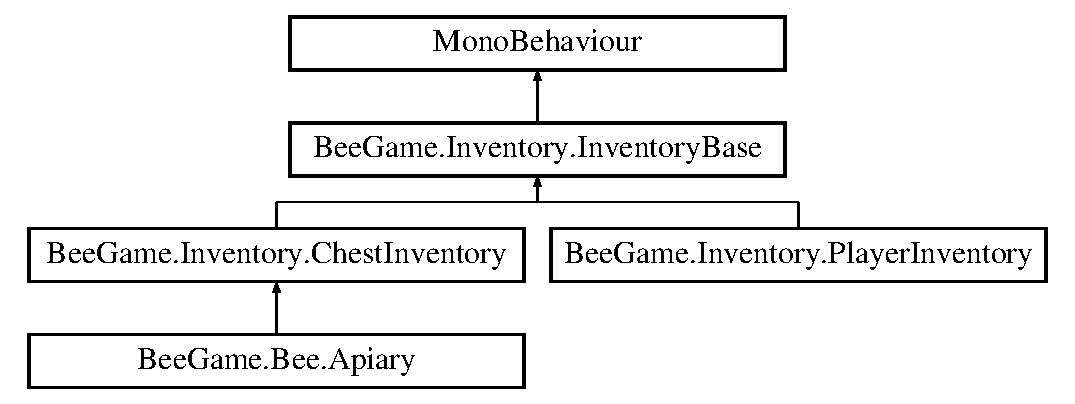
\includegraphics[height=4.000000cm]{class_bee_game_1_1_inventory_1_1_inventory_base}
\end{center}
\end{figure}
\subsection*{Public Member Functions}
\begin{DoxyCompactItemize}
\item 
void \hyperlink{class_bee_game_1_1_inventory_1_1_inventory_base_ac8edbffe8b164d66297c127654c844c4}{Update\+Slots} ()
\begin{DoxyCompactList}\small\item\em Only used when the inventory needs to be updated eg when the player is remade or when a chest is remade \end{DoxyCompactList}\end{DoxyCompactItemize}
\subsection*{Public Attributes}
\begin{DoxyCompactItemize}
\item 
\hyperlink{struct_bee_game_1_1_items_1_1_item}{Item} \hyperlink{class_bee_game_1_1_inventory_1_1_inventory_base_aa018ec0acd2aa39dd922f0a1bc1411e6}{floating\+Item}
\begin{DoxyCompactList}\small\item\em The Item that is currently being moved by the player \end{DoxyCompactList}\item 
Game\+Object \hyperlink{class_bee_game_1_1_inventory_1_1_inventory_base_af1def3187f007a5a3bb6fbe71854afdc}{item\+Info\+Pannel}
\begin{DoxyCompactList}\small\item\em Where the item\textquotesingle{}s information will show in the inventory \end{DoxyCompactList}\item 
\hyperlink{class_bee_game_1_1_inventory_1_1_inventory_slot}{Inventory\+Slot} \mbox{[}$\,$\mbox{]} \hyperlink{class_bee_game_1_1_inventory_1_1_inventory_base_a48dcba7ad7bfa1bed8c9ae290fb32857}{inventory\+G\+UI}
\begin{DoxyCompactList}\small\item\em The Unity G\+UI elements acting as the inventory slots \end{DoxyCompactList}\item 
\hyperlink{struct_bee_game_1_1_items_1_1_item}{Item} \mbox{[}$\,$\mbox{]} \hyperlink{class_bee_game_1_1_inventory_1_1_inventory_base_a405502a6eabf14e1498d96dc8aff5e8d}{slotand\+Item}
\begin{DoxyCompactList}\small\item\em The item in each of the unventory slots \end{DoxyCompactList}\end{DoxyCompactItemize}
\subsection*{Protected Member Functions}
\begin{DoxyCompactItemize}
\item 
void \hyperlink{class_bee_game_1_1_inventory_1_1_inventory_base_aa1a965cf7ba9e04b22a4ef85ad133854}{Update\+Base} ()
\begin{DoxyCompactList}\small\item\em Updates the base inventory methods as unitys Update method is hidden due to this being a parent class \end{DoxyCompactList}\item 
void \hyperlink{class_bee_game_1_1_inventory_1_1_inventory_base_aad83f463fba0efeffa7bdd2f92963ea9}{Update\+Slot\+And\+Item} ()
\begin{DoxyCompactList}\small\item\em Updates the slotand\+Item variable so their when the player is saved the inventory items are correct \end{DoxyCompactList}\end{DoxyCompactItemize}
\subsection*{Private Member Functions}
\begin{DoxyCompactItemize}
\item 
void \hyperlink{class_bee_game_1_1_inventory_1_1_inventory_base_a22d2b2a1621c8cf19925692ac8cc5923}{Start} ()
\begin{DoxyCompactList}\small\item\em Sets the parent inventory variable for each of the inventory slots \end{DoxyCompactList}\item 
void \hyperlink{class_bee_game_1_1_inventory_1_1_inventory_base_abceadbaeed5505437ba8141da8642dc7}{Update\+Item\+Display\+Data} ()
\begin{DoxyCompactList}\small\item\em Updates the item info pannel to the right hand side of the inventory \end{DoxyCompactList}\item 
void \hyperlink{class_bee_game_1_1_inventory_1_1_inventory_base_a53861c2cc0bd7af6a6569168c8866bf4}{Drop\+Item} ()
\begin{DoxyCompactList}\small\item\em Drops the item that is currently held in the floating item slot \end{DoxyCompactList}\end{DoxyCompactItemize}


\subsection{Detailed Description}


Definition at line 11 of file Inventory\+Base.\+cs.



\subsection{Member Function Documentation}
\mbox{\Hypertarget{class_bee_game_1_1_inventory_1_1_inventory_base_a53861c2cc0bd7af6a6569168c8866bf4}\label{class_bee_game_1_1_inventory_1_1_inventory_base_a53861c2cc0bd7af6a6569168c8866bf4}} 
\index{Bee\+Game\+::\+Inventory\+::\+Inventory\+Base@{Bee\+Game\+::\+Inventory\+::\+Inventory\+Base}!Drop\+Item@{Drop\+Item}}
\index{Drop\+Item@{Drop\+Item}!Bee\+Game\+::\+Inventory\+::\+Inventory\+Base@{Bee\+Game\+::\+Inventory\+::\+Inventory\+Base}}
\subsubsection{\texorpdfstring{Drop\+Item()}{DropItem()}}
{\footnotesize\ttfamily void Bee\+Game.\+Inventory.\+Inventory\+Base.\+Drop\+Item (\begin{DoxyParamCaption}{ }\end{DoxyParamCaption})\hspace{0.3cm}{\ttfamily [private]}}



Drops the item that is currently held in the floating item slot 



Definition at line 116 of file Inventory\+Base.\+cs.


\begin{DoxyCode}
117         \{
118             \textcolor{keywordflow}{if} ((Input.GetButtonDown(\textcolor{stringliteral}{"Fire1"}) || Input.GetButtonDown(\textcolor{stringliteral}{"Fire2"})) && (
      \hyperlink{class_bee_game_1_1_inventory_1_1_inventory_base_aa018ec0acd2aa39dd922f0a1bc1411e6}{floatingItem}.\hyperlink{struct_bee_game_1_1_items_1_1_item_aa85bfeab893271c26f8ca41b638ada1c}{itemId} != null && \hyperlink{class_bee_game_1_1_inventory_1_1_inventory_base_aa018ec0acd2aa39dd922f0a1bc1411e6}{floatingItem}.\hyperlink{struct_bee_game_1_1_items_1_1_item_aa85bfeab893271c26f8ca41b638ada1c}{itemId} != \textcolor{stringliteral}{""}))
119             \{
120                 \textcolor{keywordflow}{if} (!EventSystem.current.IsPointerOverGameObject())
121                 \{
122                     GameObject temp = Instantiate(\hyperlink{class_bee_game_1_1_inventory_1_1_inventory_base_aa018ec0acd2aa39dd922f0a1bc1411e6}{floatingItem}.
      \hyperlink{struct_bee_game_1_1_items_1_1_item_af28a8cd4a0eff9d4c18189c5ab525f18}{itemGameobject});
123                     temp.GetComponent<Transform>().position = transform.position;
124                     temp.GetComponent<\hyperlink{class_bee_game_1_1_items_1_1_item_game_object_interface}{ItemGameObjectInterface}>().
      \hyperlink{class_bee_game_1_1_items_1_1_item_game_object_interface_aa88fbff044f2dceb7633b1b41175d085}{UpdateItemData}(\hyperlink{class_bee_game_1_1_inventory_1_1_inventory_base_aa018ec0acd2aa39dd922f0a1bc1411e6}{floatingItem});
125                     \hyperlink{class_bee_game_1_1_inventory_1_1_inventory_base_aa018ec0acd2aa39dd922f0a1bc1411e6}{floatingItem} = \textcolor{keyword}{new} \hyperlink{struct_bee_game_1_1_items_1_1_item}{Item}();
126                 \}
127             \}
128         \}
\end{DoxyCode}
\mbox{\Hypertarget{class_bee_game_1_1_inventory_1_1_inventory_base_a22d2b2a1621c8cf19925692ac8cc5923}\label{class_bee_game_1_1_inventory_1_1_inventory_base_a22d2b2a1621c8cf19925692ac8cc5923}} 
\index{Bee\+Game\+::\+Inventory\+::\+Inventory\+Base@{Bee\+Game\+::\+Inventory\+::\+Inventory\+Base}!Start@{Start}}
\index{Start@{Start}!Bee\+Game\+::\+Inventory\+::\+Inventory\+Base@{Bee\+Game\+::\+Inventory\+::\+Inventory\+Base}}
\subsubsection{\texorpdfstring{Start()}{Start()}}
{\footnotesize\ttfamily void Bee\+Game.\+Inventory.\+Inventory\+Base.\+Start (\begin{DoxyParamCaption}{ }\end{DoxyParamCaption})\hspace{0.3cm}{\ttfamily [private]}}



Sets the parent inventory variable for each of the inventory slots 



Definition at line 33 of file Inventory\+Base.\+cs.


\begin{DoxyCode}
34         \{
35             \textcolor{keywordflow}{for} (\textcolor{keywordtype}{int} i = 0; i < \hyperlink{class_bee_game_1_1_inventory_1_1_inventory_base_a48dcba7ad7bfa1bed8c9ae290fb32857}{inventoryGUI}.Length; i++)
36             \{
37                 \hyperlink{class_bee_game_1_1_inventory_1_1_inventory_base_a48dcba7ad7bfa1bed8c9ae290fb32857}{inventoryGUI}[i].\hyperlink{class_bee_game_1_1_inventory_1_1_inventory_slot_a06c37b35f2512ee2f0652a93129808e4}{parentInventory} = \textcolor{keyword}{this};
38             \}
39         \}
\end{DoxyCode}
\mbox{\Hypertarget{class_bee_game_1_1_inventory_1_1_inventory_base_aa1a965cf7ba9e04b22a4ef85ad133854}\label{class_bee_game_1_1_inventory_1_1_inventory_base_aa1a965cf7ba9e04b22a4ef85ad133854}} 
\index{Bee\+Game\+::\+Inventory\+::\+Inventory\+Base@{Bee\+Game\+::\+Inventory\+::\+Inventory\+Base}!Update\+Base@{Update\+Base}}
\index{Update\+Base@{Update\+Base}!Bee\+Game\+::\+Inventory\+::\+Inventory\+Base@{Bee\+Game\+::\+Inventory\+::\+Inventory\+Base}}
\subsubsection{\texorpdfstring{Update\+Base()}{UpdateBase()}}
{\footnotesize\ttfamily void Bee\+Game.\+Inventory.\+Inventory\+Base.\+Update\+Base (\begin{DoxyParamCaption}{ }\end{DoxyParamCaption})\hspace{0.3cm}{\ttfamily [protected]}}



Updates the base inventory methods as unitys Update method is hidden due to this being a parent class 



Definition at line 44 of file Inventory\+Base.\+cs.


\begin{DoxyCode}
45         \{
46             \hyperlink{class_bee_game_1_1_inventory_1_1_inventory_base_aad83f463fba0efeffa7bdd2f92963ea9}{UpdateSlotAndItem}();
47             \hyperlink{class_bee_game_1_1_inventory_1_1_inventory_base_a53861c2cc0bd7af6a6569168c8866bf4}{DropItem}();
48             \hyperlink{class_bee_game_1_1_inventory_1_1_inventory_base_abceadbaeed5505437ba8141da8642dc7}{UpdateItemDisplayData}();
49         \}
\end{DoxyCode}
\mbox{\Hypertarget{class_bee_game_1_1_inventory_1_1_inventory_base_abceadbaeed5505437ba8141da8642dc7}\label{class_bee_game_1_1_inventory_1_1_inventory_base_abceadbaeed5505437ba8141da8642dc7}} 
\index{Bee\+Game\+::\+Inventory\+::\+Inventory\+Base@{Bee\+Game\+::\+Inventory\+::\+Inventory\+Base}!Update\+Item\+Display\+Data@{Update\+Item\+Display\+Data}}
\index{Update\+Item\+Display\+Data@{Update\+Item\+Display\+Data}!Bee\+Game\+::\+Inventory\+::\+Inventory\+Base@{Bee\+Game\+::\+Inventory\+::\+Inventory\+Base}}
\subsubsection{\texorpdfstring{Update\+Item\+Display\+Data()}{UpdateItemDisplayData()}}
{\footnotesize\ttfamily void Bee\+Game.\+Inventory.\+Inventory\+Base.\+Update\+Item\+Display\+Data (\begin{DoxyParamCaption}{ }\end{DoxyParamCaption})\hspace{0.3cm}{\ttfamily [private]}}



Updates the item info pannel to the right hand side of the inventory 



Definition at line 54 of file Inventory\+Base.\+cs.


\begin{DoxyCode}
55         \{
56             \textcolor{keywordflow}{if}(\hyperlink{class_bee_game_1_1_inventory_1_1_inventory_base_aa018ec0acd2aa39dd922f0a1bc1411e6}{floatingItem}.\hyperlink{struct_bee_game_1_1_items_1_1_item_aa85bfeab893271c26f8ca41b638ada1c}{itemId} != \textcolor{stringliteral}{""} && \hyperlink{class_bee_game_1_1_inventory_1_1_inventory_base_aa018ec0acd2aa39dd922f0a1bc1411e6}{floatingItem}.
      \hyperlink{struct_bee_game_1_1_items_1_1_item_aa85bfeab893271c26f8ca41b638ada1c}{itemId} != null)
57             \{
58                 Text[] infoPannnelTexts = \hyperlink{class_bee_game_1_1_inventory_1_1_inventory_base_af1def3187f007a5a3bb6fbe71854afdc}{itemInfoPannel}.GetComponentsInChildren<Text>();
59 
60                 infoPannnelTexts[0].text = \hyperlink{class_bee_game_1_1_inventory_1_1_inventory_base_aa018ec0acd2aa39dd922f0a1bc1411e6}{floatingItem}.\hyperlink{struct_bee_game_1_1_items_1_1_item_a0b0bd7eb510757f650f1be3d05b23fc8}{name};
61                 \textcolor{keywordflow}{if} (\hyperlink{class_bee_game_1_1_inventory_1_1_inventory_base_aa018ec0acd2aa39dd922f0a1bc1411e6}{floatingItem}.\hyperlink{struct_bee_game_1_1_items_1_1_item_a0593f3b7b3ff5daa864f3c6d0ccd77ca}{beeItem} != null)
62                 \{
63                     \textcolor{keywordflow}{if}(\hyperlink{class_bee_game_1_1_inventory_1_1_inventory_base_aa018ec0acd2aa39dd922f0a1bc1411e6}{floatingItem}.\hyperlink{struct_bee_game_1_1_items_1_1_item_a59ee527a4e9cd5b3e0ed2ec30f248a28}{CanSeeBeeData}())
64                     \{
65                         infoPannnelTexts[1].text = \hyperlink{class_bee_game_1_1_inventory_1_1_inventory_base_aa018ec0acd2aa39dd922f0a1bc1411e6}{floatingItem}.
      \hyperlink{struct_bee_game_1_1_items_1_1_item_a1c2f63541269f310381704fc7cc5bc5d}{ReturnBeeDataAsText}();
66                     \}
67                     \textcolor{keywordflow}{else}
68                     \{
69                         infoPannnelTexts[1].text = \hyperlink{class_bee_game_1_1_inventory_1_1_inventory_base_aa018ec0acd2aa39dd922f0a1bc1411e6}{floatingItem}.
      \hyperlink{struct_bee_game_1_1_items_1_1_item_a3173b5fb0a51e9063335e5cbf93c2e1b}{description};
70                     \}
71                 \}
72                 \textcolor{keywordflow}{else}
73                 \{
74                     infoPannnelTexts[1].text = \hyperlink{class_bee_game_1_1_inventory_1_1_inventory_base_aa018ec0acd2aa39dd922f0a1bc1411e6}{floatingItem}.
      \hyperlink{struct_bee_game_1_1_items_1_1_item_a3173b5fb0a51e9063335e5cbf93c2e1b}{description};
75                 \}
76             \}
77         \}
\end{DoxyCode}
\mbox{\Hypertarget{class_bee_game_1_1_inventory_1_1_inventory_base_aad83f463fba0efeffa7bdd2f92963ea9}\label{class_bee_game_1_1_inventory_1_1_inventory_base_aad83f463fba0efeffa7bdd2f92963ea9}} 
\index{Bee\+Game\+::\+Inventory\+::\+Inventory\+Base@{Bee\+Game\+::\+Inventory\+::\+Inventory\+Base}!Update\+Slot\+And\+Item@{Update\+Slot\+And\+Item}}
\index{Update\+Slot\+And\+Item@{Update\+Slot\+And\+Item}!Bee\+Game\+::\+Inventory\+::\+Inventory\+Base@{Bee\+Game\+::\+Inventory\+::\+Inventory\+Base}}
\subsubsection{\texorpdfstring{Update\+Slot\+And\+Item()}{UpdateSlotAndItem()}}
{\footnotesize\ttfamily void Bee\+Game.\+Inventory.\+Inventory\+Base.\+Update\+Slot\+And\+Item (\begin{DoxyParamCaption}{ }\end{DoxyParamCaption})\hspace{0.3cm}{\ttfamily [protected]}}



Updates the slotand\+Item variable so their when the player is saved the inventory items are correct 



Definition at line 82 of file Inventory\+Base.\+cs.


\begin{DoxyCode}
83         \{
84             \textcolor{keywordflow}{if}(\hyperlink{class_bee_game_1_1_inventory_1_1_inventory_base_a405502a6eabf14e1498d96dc8aff5e8d}{slotandItem} == null)
85             \{
86                 \hyperlink{class_bee_game_1_1_inventory_1_1_inventory_base_a405502a6eabf14e1498d96dc8aff5e8d}{slotandItem} = \textcolor{keyword}{new} \hyperlink{struct_bee_game_1_1_items_1_1_item}{Item}[\hyperlink{class_bee_game_1_1_inventory_1_1_inventory_base_a48dcba7ad7bfa1bed8c9ae290fb32857}{inventoryGUI}.Length];
87             \}
88 
89             \textcolor{keywordflow}{if}(\hyperlink{class_bee_game_1_1_inventory_1_1_inventory_base_a405502a6eabf14e1498d96dc8aff5e8d}{slotandItem}.Length  < \hyperlink{class_bee_game_1_1_inventory_1_1_inventory_base_a48dcba7ad7bfa1bed8c9ae290fb32857}{inventoryGUI}.Length)
90             \{
91                 \hyperlink{class_bee_game_1_1_inventory_1_1_inventory_base_a405502a6eabf14e1498d96dc8aff5e8d}{slotandItem} = \textcolor{keyword}{new} \hyperlink{struct_bee_game_1_1_items_1_1_item}{Item}[\hyperlink{class_bee_game_1_1_inventory_1_1_inventory_base_a48dcba7ad7bfa1bed8c9ae290fb32857}{inventoryGUI}.Length];
92             \}
93 
94             \textcolor{keywordflow}{for} (\textcolor{keywordtype}{int} i = 0; i < \hyperlink{class_bee_game_1_1_inventory_1_1_inventory_base_a48dcba7ad7bfa1bed8c9ae290fb32857}{inventoryGUI}.Length; i++)
95             \{
96                 \hyperlink{class_bee_game_1_1_inventory_1_1_inventory_base_a405502a6eabf14e1498d96dc8aff5e8d}{slotandItem}[i] = \hyperlink{class_bee_game_1_1_inventory_1_1_inventory_base_a48dcba7ad7bfa1bed8c9ae290fb32857}{inventoryGUI}[i].\hyperlink{class_bee_game_1_1_inventory_1_1_inventory_slot_a31b201e7eef9ed0001a447b3f76a7a81}{item};
97             \}
98         \}
\end{DoxyCode}
\mbox{\Hypertarget{class_bee_game_1_1_inventory_1_1_inventory_base_ac8edbffe8b164d66297c127654c844c4}\label{class_bee_game_1_1_inventory_1_1_inventory_base_ac8edbffe8b164d66297c127654c844c4}} 
\index{Bee\+Game\+::\+Inventory\+::\+Inventory\+Base@{Bee\+Game\+::\+Inventory\+::\+Inventory\+Base}!Update\+Slots@{Update\+Slots}}
\index{Update\+Slots@{Update\+Slots}!Bee\+Game\+::\+Inventory\+::\+Inventory\+Base@{Bee\+Game\+::\+Inventory\+::\+Inventory\+Base}}
\subsubsection{\texorpdfstring{Update\+Slots()}{UpdateSlots()}}
{\footnotesize\ttfamily void Bee\+Game.\+Inventory.\+Inventory\+Base.\+Update\+Slots (\begin{DoxyParamCaption}{ }\end{DoxyParamCaption})}



Only used when the inventory needs to be updated eg when the player is remade or when a chest is remade 



Definition at line 103 of file Inventory\+Base.\+cs.


\begin{DoxyCode}
104         \{
105             \hyperlink{class_bee_game_1_1_inventory_1_1_inventory_base_a22d2b2a1621c8cf19925692ac8cc5923}{Start}();
106             \textcolor{keywordflow}{for} (\textcolor{keywordtype}{int} i = 0; i < \hyperlink{class_bee_game_1_1_inventory_1_1_inventory_base_a48dcba7ad7bfa1bed8c9ae290fb32857}{inventoryGUI}.Length; i++)
107             \{
108                 \hyperlink{class_bee_game_1_1_inventory_1_1_inventory_base_a48dcba7ad7bfa1bed8c9ae290fb32857}{inventoryGUI}[i].\hyperlink{class_bee_game_1_1_inventory_1_1_inventory_slot_a31b201e7eef9ed0001a447b3f76a7a81}{item} = \hyperlink{class_bee_game_1_1_inventory_1_1_inventory_base_a405502a6eabf14e1498d96dc8aff5e8d}{slotandItem}[i];
109                 \hyperlink{class_bee_game_1_1_inventory_1_1_inventory_base_a48dcba7ad7bfa1bed8c9ae290fb32857}{inventoryGUI}[i].\hyperlink{class_bee_game_1_1_inventory_1_1_inventory_slot_a31b201e7eef9ed0001a447b3f76a7a81}{item}.\hyperlink{struct_bee_game_1_1_items_1_1_item_a29abdb5010a23262e7562720bb85c171}{UpdateSpriteAndObject}();
110             \}
111         \}
\end{DoxyCode}


\subsection{Member Data Documentation}
\mbox{\Hypertarget{class_bee_game_1_1_inventory_1_1_inventory_base_aa018ec0acd2aa39dd922f0a1bc1411e6}\label{class_bee_game_1_1_inventory_1_1_inventory_base_aa018ec0acd2aa39dd922f0a1bc1411e6}} 
\index{Bee\+Game\+::\+Inventory\+::\+Inventory\+Base@{Bee\+Game\+::\+Inventory\+::\+Inventory\+Base}!floating\+Item@{floating\+Item}}
\index{floating\+Item@{floating\+Item}!Bee\+Game\+::\+Inventory\+::\+Inventory\+Base@{Bee\+Game\+::\+Inventory\+::\+Inventory\+Base}}
\subsubsection{\texorpdfstring{floating\+Item}{floatingItem}}
{\footnotesize\ttfamily \hyperlink{struct_bee_game_1_1_items_1_1_item}{Item} Bee\+Game.\+Inventory.\+Inventory\+Base.\+floating\+Item}



The Item that is currently being moved by the player 



Definition at line 16 of file Inventory\+Base.\+cs.

\mbox{\Hypertarget{class_bee_game_1_1_inventory_1_1_inventory_base_a48dcba7ad7bfa1bed8c9ae290fb32857}\label{class_bee_game_1_1_inventory_1_1_inventory_base_a48dcba7ad7bfa1bed8c9ae290fb32857}} 
\index{Bee\+Game\+::\+Inventory\+::\+Inventory\+Base@{Bee\+Game\+::\+Inventory\+::\+Inventory\+Base}!inventory\+G\+UI@{inventory\+G\+UI}}
\index{inventory\+G\+UI@{inventory\+G\+UI}!Bee\+Game\+::\+Inventory\+::\+Inventory\+Base@{Bee\+Game\+::\+Inventory\+::\+Inventory\+Base}}
\subsubsection{\texorpdfstring{inventory\+G\+UI}{inventoryGUI}}
{\footnotesize\ttfamily \hyperlink{class_bee_game_1_1_inventory_1_1_inventory_slot}{Inventory\+Slot} \mbox{[}$\,$\mbox{]} Bee\+Game.\+Inventory.\+Inventory\+Base.\+inventory\+G\+UI}



The Unity G\+UI elements acting as the inventory slots 



Definition at line 24 of file Inventory\+Base.\+cs.

\mbox{\Hypertarget{class_bee_game_1_1_inventory_1_1_inventory_base_af1def3187f007a5a3bb6fbe71854afdc}\label{class_bee_game_1_1_inventory_1_1_inventory_base_af1def3187f007a5a3bb6fbe71854afdc}} 
\index{Bee\+Game\+::\+Inventory\+::\+Inventory\+Base@{Bee\+Game\+::\+Inventory\+::\+Inventory\+Base}!item\+Info\+Pannel@{item\+Info\+Pannel}}
\index{item\+Info\+Pannel@{item\+Info\+Pannel}!Bee\+Game\+::\+Inventory\+::\+Inventory\+Base@{Bee\+Game\+::\+Inventory\+::\+Inventory\+Base}}
\subsubsection{\texorpdfstring{item\+Info\+Pannel}{itemInfoPannel}}
{\footnotesize\ttfamily Game\+Object Bee\+Game.\+Inventory.\+Inventory\+Base.\+item\+Info\+Pannel}



Where the item\textquotesingle{}s information will show in the inventory 



Definition at line 20 of file Inventory\+Base.\+cs.

\mbox{\Hypertarget{class_bee_game_1_1_inventory_1_1_inventory_base_a405502a6eabf14e1498d96dc8aff5e8d}\label{class_bee_game_1_1_inventory_1_1_inventory_base_a405502a6eabf14e1498d96dc8aff5e8d}} 
\index{Bee\+Game\+::\+Inventory\+::\+Inventory\+Base@{Bee\+Game\+::\+Inventory\+::\+Inventory\+Base}!slotand\+Item@{slotand\+Item}}
\index{slotand\+Item@{slotand\+Item}!Bee\+Game\+::\+Inventory\+::\+Inventory\+Base@{Bee\+Game\+::\+Inventory\+::\+Inventory\+Base}}
\subsubsection{\texorpdfstring{slotand\+Item}{slotandItem}}
{\footnotesize\ttfamily \hyperlink{struct_bee_game_1_1_items_1_1_item}{Item} \mbox{[}$\,$\mbox{]} Bee\+Game.\+Inventory.\+Inventory\+Base.\+slotand\+Item}



The item in each of the unventory slots 



Definition at line 28 of file Inventory\+Base.\+cs.



The documentation for this class was generated from the following file\+:\begin{DoxyCompactItemize}
\item 
C\+:/\+Users/\+Toothless/\+Documents/\+Git\+Hub/\+Bee\+Game/\+Code/\+Bee\+Game/\+Bee\+Game/\+Inventory/\hyperlink{_inventory_base_8cs}{Inventory\+Base.\+cs}\end{DoxyCompactItemize}

\hypertarget{class_bee_game_1_1_inventory_1_1_inventory_slot}{}\section{Bee\+Game.\+Inventory.\+Inventory\+Slot Class Reference}
\label{class_bee_game_1_1_inventory_1_1_inventory_slot}\index{Bee\+Game.\+Inventory.\+Inventory\+Slot@{Bee\+Game.\+Inventory.\+Inventory\+Slot}}
Inheritance diagram for Bee\+Game.\+Inventory.\+Inventory\+Slot\+:\begin{figure}[H]
\begin{center}
\leavevmode
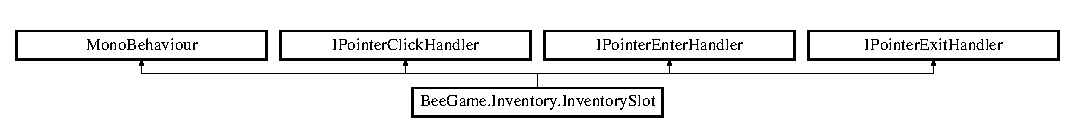
\includegraphics[height=1.339713cm]{class_bee_game_1_1_inventory_1_1_inventory_slot}
\end{center}
\end{figure}
\subsection*{Public Member Functions}
\begin{DoxyCompactItemize}
\item 
void \hyperlink{class_bee_game_1_1_inventory_1_1_inventory_slot_a471790f0d1eb55a483b0a530c6371c09}{On\+Pointer\+Enter} (Pointer\+Event\+Data event\+Data)
\begin{DoxyCompactList}\small\item\em Updates the side pannel to show the items data \end{DoxyCompactList}\item 
void \hyperlink{class_bee_game_1_1_inventory_1_1_inventory_slot_a13a4046ae2c80a52f3b1ed44fc1a5ef1}{On\+Pointer\+Exit} (Pointer\+Event\+Data event\+Data)
\begin{DoxyCompactList}\small\item\em Removes the items data from the item data desplay pannel \end{DoxyCompactList}\item 
void \hyperlink{class_bee_game_1_1_inventory_1_1_inventory_slot_abe33997cbde05772253494f20f949483}{Update\+Graphic} ()
\begin{DoxyCompactList}\small\item\em Updates the graphic on the slot G\+UI \end{DoxyCompactList}\item 
void \hyperlink{class_bee_game_1_1_inventory_1_1_inventory_slot_adc03a9101c901f82a3dfc778db98cf1f}{Update\+Selected\+Slot} (bool selected)
\begin{DoxyCompactList}\small\item\em Only used for the hotbar item slots \end{DoxyCompactList}\item 
void \hyperlink{class_bee_game_1_1_inventory_1_1_inventory_slot_a582545a412e4b746be55d36a11e61e96}{On\+Pointer\+Click} (Pointer\+Event\+Data event\+Data)
\begin{DoxyCompactList}\small\item\em When the slot is clicked this is called. Controlls how an item is moved around the inventory \end{DoxyCompactList}\end{DoxyCompactItemize}
\subsection*{Public Attributes}
\begin{DoxyCompactItemize}
\item 
bool \hyperlink{class_bee_game_1_1_inventory_1_1_inventory_slot_a249f89b637bf8cdb83785b68ce617b4c}{can\+Place\+Object\+In\+Slot} = true
\begin{DoxyCompactList}\small\item\em Can an Item be place into the inventory slot by the player? Default = true \end{DoxyCompactList}\item 
\hyperlink{class_bee_game_1_1_inventory_1_1_inventory_base}{Inventory\+Base} \hyperlink{class_bee_game_1_1_inventory_1_1_inventory_slot_a06c37b35f2512ee2f0652a93129808e4}{parent\+Inventory}
\begin{DoxyCompactList}\small\item\em The inventory that is slot is attached to \hyperlink{class_bee_game_1_1_inventory_1_1_inventory_base}{Inventory\+Base} \end{DoxyCompactList}\item 
Text \hyperlink{class_bee_game_1_1_inventory_1_1_inventory_slot_adbdcece869818ee00193cf27bd9f46d4}{number}
\begin{DoxyCompactList}\small\item\em The Unity G\+UI Text element that will display the stack count number \end{DoxyCompactList}\item 
Game\+Object \hyperlink{class_bee_game_1_1_inventory_1_1_inventory_slot_aa45b9de343c847b7c8d7db4163f765ec}{item\+Info\+Pannel}
\begin{DoxyCompactList}\small\item\em The item info pannel where the item data should be displayed \end{DoxyCompactList}\item 
\hyperlink{struct_bee_game_1_1_items_1_1_item}{Item} \hyperlink{class_bee_game_1_1_inventory_1_1_inventory_slot_a31b201e7eef9ed0001a447b3f76a7a81}{item}
\begin{DoxyCompactList}\small\item\em The item in the slot \end{DoxyCompactList}\end{DoxyCompactItemize}
\subsection*{Private Member Functions}
\begin{DoxyCompactItemize}
\item 
void \hyperlink{class_bee_game_1_1_inventory_1_1_inventory_slot_ae5fe19d6bdefd8c6ceb6800bba276f93}{Start} ()
\item 
void \hyperlink{class_bee_game_1_1_inventory_1_1_inventory_slot_a30c6d192daefd9e7108cad1bafda814a}{Update} ()
\begin{DoxyCompactList}\small\item\em Updates the slot every frame, when it is being viewed \end{DoxyCompactList}\item 
void \hyperlink{class_bee_game_1_1_inventory_1_1_inventory_slot_a58cc9b63c6af1dceccee17210b73f70d}{Update\+Stack\+Number} ()
\begin{DoxyCompactList}\small\item\em Updates the stack number on the G\+UI \end{DoxyCompactList}\end{DoxyCompactItemize}
\subsection*{Private Attributes}
\begin{DoxyCompactItemize}
\item 
bool \hyperlink{class_bee_game_1_1_inventory_1_1_inventory_slot_a3c2a56594821f0567448a541b1236961}{is\+Selected}
\begin{DoxyCompactList}\small\item\em Is this slot currently selected in the hotbar (Default = False) \end{DoxyCompactList}\end{DoxyCompactItemize}


\subsection{Detailed Description}


Definition at line 10 of file Inventory\+Slot.\+cs.



\subsection{Member Function Documentation}
\mbox{\Hypertarget{class_bee_game_1_1_inventory_1_1_inventory_slot_a582545a412e4b746be55d36a11e61e96}\label{class_bee_game_1_1_inventory_1_1_inventory_slot_a582545a412e4b746be55d36a11e61e96}} 
\index{Bee\+Game\+::\+Inventory\+::\+Inventory\+Slot@{Bee\+Game\+::\+Inventory\+::\+Inventory\+Slot}!On\+Pointer\+Click@{On\+Pointer\+Click}}
\index{On\+Pointer\+Click@{On\+Pointer\+Click}!Bee\+Game\+::\+Inventory\+::\+Inventory\+Slot@{Bee\+Game\+::\+Inventory\+::\+Inventory\+Slot}}
\subsubsection{\texorpdfstring{On\+Pointer\+Click()}{OnPointerClick()}}
{\footnotesize\ttfamily void Bee\+Game.\+Inventory.\+Inventory\+Slot.\+On\+Pointer\+Click (\begin{DoxyParamCaption}\item[{Pointer\+Event\+Data}]{event\+Data }\end{DoxyParamCaption})}



When the slot is clicked this is called. Controlls how an item is moved around the inventory 


\begin{DoxyParams}{Parameters}
{\em event\+Data} & Right, Left, or Middle click\\
\hline
\end{DoxyParams}


Definition at line 176 of file Inventory\+Slot.\+cs.


\begin{DoxyCode}
177         \{
178             \textcolor{keywordflow}{if} (eventData.button == PointerEventData.InputButton.Left)
179             \{
180                 \textcolor{comment}{//if their is something in the item slot}
181                 \textcolor{keywordflow}{if} (\hyperlink{class_bee_game_1_1_inventory_1_1_inventory_slot_a31b201e7eef9ed0001a447b3f76a7a81}{item}.\hyperlink{struct_bee_game_1_1_items_1_1_item_aa85bfeab893271c26f8ca41b638ada1c}{itemId} != \textcolor{stringliteral}{""} && \hyperlink{class_bee_game_1_1_inventory_1_1_inventory_slot_a31b201e7eef9ed0001a447b3f76a7a81}{item}.\hyperlink{struct_bee_game_1_1_items_1_1_item_aa85bfeab893271c26f8ca41b638ada1c}{itemId} != null)
182                 \{
183                     \textcolor{comment}{//if their is somethign in the floating item}
184                     \textcolor{keywordflow}{if} (\hyperlink{class_bee_game_1_1_inventory_1_1_inventory_slot_a06c37b35f2512ee2f0652a93129808e4}{parentInventory}.\hyperlink{class_bee_game_1_1_inventory_1_1_inventory_base_aa018ec0acd2aa39dd922f0a1bc1411e6}{floatingItem}.
      \hyperlink{struct_bee_game_1_1_items_1_1_item_aa85bfeab893271c26f8ca41b638ada1c}{itemId} != \textcolor{stringliteral}{""} && \hyperlink{class_bee_game_1_1_inventory_1_1_inventory_slot_a06c37b35f2512ee2f0652a93129808e4}{parentInventory}.\hyperlink{class_bee_game_1_1_inventory_1_1_inventory_base_aa018ec0acd2aa39dd922f0a1bc1411e6}{floatingItem}.
      \hyperlink{struct_bee_game_1_1_items_1_1_item_aa85bfeab893271c26f8ca41b638ada1c}{itemId} != null)
185                     \{
186                         \textcolor{comment}{//if something can be place into the slot}
187                         \textcolor{keywordflow}{if} (\hyperlink{class_bee_game_1_1_inventory_1_1_inventory_slot_a249f89b637bf8cdb83785b68ce617b4c}{canPlaceObjectInSlot})
188                         \{
189                             \textcolor{comment}{//if items in both the slot and floating item are the same}
190                             \textcolor{keywordflow}{if} (\hyperlink{class_bee_game_1_1_inventory_1_1_inventory_slot_a31b201e7eef9ed0001a447b3f76a7a81}{item} == \hyperlink{class_bee_game_1_1_inventory_1_1_inventory_slot_a06c37b35f2512ee2f0652a93129808e4}{parentInventory}.
      \hyperlink{class_bee_game_1_1_inventory_1_1_inventory_base_aa018ec0acd2aa39dd922f0a1bc1411e6}{floatingItem})
191                             \{
192                                 \textcolor{keywordflow}{if} (\hyperlink{class_bee_game_1_1_inventory_1_1_inventory_slot_a31b201e7eef9ed0001a447b3f76a7a81}{item}.\hyperlink{struct_bee_game_1_1_items_1_1_item_aaa169917b0e0f8472f20398d5d448388}{stackCount} + 
      \hyperlink{class_bee_game_1_1_inventory_1_1_inventory_slot_a06c37b35f2512ee2f0652a93129808e4}{parentInventory}.\hyperlink{class_bee_game_1_1_inventory_1_1_inventory_base_aa018ec0acd2aa39dd922f0a1bc1411e6}{floatingItem}.\hyperlink{struct_bee_game_1_1_items_1_1_item_aaa169917b0e0f8472f20398d5d448388}{stackCount} < 
      \hyperlink{class_bee_game_1_1_inventory_1_1_inventory_slot_a31b201e7eef9ed0001a447b3f76a7a81}{item}.\hyperlink{struct_bee_game_1_1_items_1_1_item_a045f162bbb378f44e8b89af901b29ff3}{maxStackCount} + 1)
193                                 \{
194                                     \hyperlink{class_bee_game_1_1_inventory_1_1_inventory_slot_a31b201e7eef9ed0001a447b3f76a7a81}{item}.\hyperlink{struct_bee_game_1_1_items_1_1_item_aaa169917b0e0f8472f20398d5d448388}{stackCount} += 
      \hyperlink{class_bee_game_1_1_inventory_1_1_inventory_slot_a06c37b35f2512ee2f0652a93129808e4}{parentInventory}.\hyperlink{class_bee_game_1_1_inventory_1_1_inventory_base_aa018ec0acd2aa39dd922f0a1bc1411e6}{floatingItem}.\hyperlink{struct_bee_game_1_1_items_1_1_item_aaa169917b0e0f8472f20398d5d448388}{stackCount};
195                                     \hyperlink{class_bee_game_1_1_inventory_1_1_inventory_slot_a06c37b35f2512ee2f0652a93129808e4}{parentInventory}.\hyperlink{class_bee_game_1_1_inventory_1_1_inventory_base_aa018ec0acd2aa39dd922f0a1bc1411e6}{floatingItem} = \textcolor{keyword}{new} 
      \hyperlink{struct_bee_game_1_1_items_1_1_item}{Item}();
196                                 \}
197                                 \textcolor{keywordflow}{else}
198                                 \{
199                                     \textcolor{comment}{//if neither of the stacks are full but both of them added are more
       than the max stack count}
200                                     \textcolor{keywordflow}{if} (\hyperlink{class_bee_game_1_1_inventory_1_1_inventory_slot_a06c37b35f2512ee2f0652a93129808e4}{parentInventory}.
      \hyperlink{class_bee_game_1_1_inventory_1_1_inventory_base_aa018ec0acd2aa39dd922f0a1bc1411e6}{floatingItem}.\hyperlink{struct_bee_game_1_1_items_1_1_item_aaa169917b0e0f8472f20398d5d448388}{stackCount} != \hyperlink{class_bee_game_1_1_inventory_1_1_inventory_slot_a31b201e7eef9ed0001a447b3f76a7a81}{item}.\hyperlink{struct_bee_game_1_1_items_1_1_item_a045f162bbb378f44e8b89af901b29ff3}{maxStackCount} && 
      \hyperlink{class_bee_game_1_1_inventory_1_1_inventory_slot_a31b201e7eef9ed0001a447b3f76a7a81}{item}.\hyperlink{struct_bee_game_1_1_items_1_1_item_aaa169917b0e0f8472f20398d5d448388}{stackCount} != \hyperlink{class_bee_game_1_1_inventory_1_1_inventory_slot_a31b201e7eef9ed0001a447b3f76a7a81}{item}.\hyperlink{struct_bee_game_1_1_items_1_1_item_a045f162bbb378f44e8b89af901b29ff3}{maxStackCount})
201                                     \{
202                                         \textcolor{keywordtype}{int} \textcolor{keyword}{remove} = (\hyperlink{class_bee_game_1_1_inventory_1_1_inventory_slot_a31b201e7eef9ed0001a447b3f76a7a81}{item}.\hyperlink{struct_bee_game_1_1_items_1_1_item_aaa169917b0e0f8472f20398d5d448388}{stackCount} + 
      \hyperlink{class_bee_game_1_1_inventory_1_1_inventory_slot_a06c37b35f2512ee2f0652a93129808e4}{parentInventory}.\hyperlink{class_bee_game_1_1_inventory_1_1_inventory_base_aa018ec0acd2aa39dd922f0a1bc1411e6}{floatingItem}.\hyperlink{struct_bee_game_1_1_items_1_1_item_aaa169917b0e0f8472f20398d5d448388}{stackCount}) - 
      \hyperlink{class_bee_game_1_1_inventory_1_1_inventory_slot_a31b201e7eef9ed0001a447b3f76a7a81}{item}.\hyperlink{struct_bee_game_1_1_items_1_1_item_a045f162bbb378f44e8b89af901b29ff3}{maxStackCount};
203                                         \hyperlink{class_bee_game_1_1_inventory_1_1_inventory_slot_a31b201e7eef9ed0001a447b3f76a7a81}{item}.\hyperlink{struct_bee_game_1_1_items_1_1_item_aaa169917b0e0f8472f20398d5d448388}{stackCount} = \hyperlink{class_bee_game_1_1_inventory_1_1_inventory_slot_a31b201e7eef9ed0001a447b3f76a7a81}{item}.
      \hyperlink{struct_bee_game_1_1_items_1_1_item_a045f162bbb378f44e8b89af901b29ff3}{maxStackCount};
204                                         \hyperlink{class_bee_game_1_1_inventory_1_1_inventory_slot_a06c37b35f2512ee2f0652a93129808e4}{parentInventory}.
      \hyperlink{class_bee_game_1_1_inventory_1_1_inventory_base_aa018ec0acd2aa39dd922f0a1bc1411e6}{floatingItem}.\hyperlink{struct_bee_game_1_1_items_1_1_item_aaa169917b0e0f8472f20398d5d448388}{stackCount} -= \textcolor{keyword}{remove};
205 
206                                         if (\hyperlink{class_bee_game_1_1_inventory_1_1_inventory_slot_a06c37b35f2512ee2f0652a93129808e4}{parentInventory}.
      \hyperlink{class_bee_game_1_1_inventory_1_1_inventory_base_aa018ec0acd2aa39dd922f0a1bc1411e6}{floatingItem}.\hyperlink{struct_bee_game_1_1_items_1_1_item_aaa169917b0e0f8472f20398d5d448388}{stackCount} < 1)
207                                         \{
208                                             \hyperlink{class_bee_game_1_1_inventory_1_1_inventory_slot_a06c37b35f2512ee2f0652a93129808e4}{parentInventory}.
      \hyperlink{class_bee_game_1_1_inventory_1_1_inventory_base_aa018ec0acd2aa39dd922f0a1bc1411e6}{floatingItem} = \textcolor{keyword}{new} \hyperlink{struct_bee_game_1_1_items_1_1_item}{Item}();
209                                         \}
210                                     \}
211                                     \textcolor{comment}{//if both stacks are full swap the stacks}
212                                     \textcolor{keywordflow}{else}
213                                     \{
214                                         \hyperlink{struct_bee_game_1_1_items_1_1_item}{Item} temp = \hyperlink{class_bee_game_1_1_inventory_1_1_inventory_slot_a31b201e7eef9ed0001a447b3f76a7a81}{item};
215                                         \hyperlink{class_bee_game_1_1_inventory_1_1_inventory_slot_a31b201e7eef9ed0001a447b3f76a7a81}{item} = \hyperlink{class_bee_game_1_1_inventory_1_1_inventory_slot_a06c37b35f2512ee2f0652a93129808e4}{parentInventory}.
      \hyperlink{class_bee_game_1_1_inventory_1_1_inventory_base_aa018ec0acd2aa39dd922f0a1bc1411e6}{floatingItem};
216                                         \hyperlink{class_bee_game_1_1_inventory_1_1_inventory_slot_a06c37b35f2512ee2f0652a93129808e4}{parentInventory}.
      \hyperlink{class_bee_game_1_1_inventory_1_1_inventory_base_aa018ec0acd2aa39dd922f0a1bc1411e6}{floatingItem} = temp;
217                                     \}
218                                 \}
219                             \}
220                             \textcolor{comment}{//if the items are not the same swap them}
221                             \textcolor{keywordflow}{else}
222                             \{
223                                 \hyperlink{struct_bee_game_1_1_items_1_1_item}{Item} temp = \hyperlink{class_bee_game_1_1_inventory_1_1_inventory_slot_a31b201e7eef9ed0001a447b3f76a7a81}{item};
224                                 \hyperlink{class_bee_game_1_1_inventory_1_1_inventory_slot_a31b201e7eef9ed0001a447b3f76a7a81}{item} = \hyperlink{class_bee_game_1_1_inventory_1_1_inventory_slot_a06c37b35f2512ee2f0652a93129808e4}{parentInventory}.
      \hyperlink{class_bee_game_1_1_inventory_1_1_inventory_base_aa018ec0acd2aa39dd922f0a1bc1411e6}{floatingItem};
225                                 \hyperlink{class_bee_game_1_1_inventory_1_1_inventory_slot_a06c37b35f2512ee2f0652a93129808e4}{parentInventory}.\hyperlink{class_bee_game_1_1_inventory_1_1_inventory_base_aa018ec0acd2aa39dd922f0a1bc1411e6}{floatingItem} = temp;
226                             \}
227                         \}
228                     \}
229                     \textcolor{comment}{//if their isn't something in the floting item copy this slots item in to it and empty
       the slot}
230                     \textcolor{keywordflow}{else}
231                     \{
232                         \hyperlink{class_bee_game_1_1_inventory_1_1_inventory_slot_a06c37b35f2512ee2f0652a93129808e4}{parentInventory}.\hyperlink{class_bee_game_1_1_inventory_1_1_inventory_base_aa018ec0acd2aa39dd922f0a1bc1411e6}{floatingItem} = 
      \hyperlink{class_bee_game_1_1_inventory_1_1_inventory_slot_a31b201e7eef9ed0001a447b3f76a7a81}{item};
233                         \hyperlink{class_bee_game_1_1_inventory_1_1_inventory_slot_a31b201e7eef9ed0001a447b3f76a7a81}{item} = \textcolor{keyword}{new} \hyperlink{struct_bee_game_1_1_items_1_1_item}{Item}();
234                     \}
235                 \}
236                 \textcolor{keywordflow}{else}
237                 \{
238                     \textcolor{comment}{//if something can be place into the slot}
239                     \textcolor{keywordflow}{if}(\hyperlink{class_bee_game_1_1_inventory_1_1_inventory_slot_a249f89b637bf8cdb83785b68ce617b4c}{canPlaceObjectInSlot})
240                     \{
241                         \textcolor{comment}{//if their isnt something in the slot but ther is something in the floting item put
       floting item into the slot and empty the floating item }
242                         \textcolor{keywordflow}{if} (\hyperlink{class_bee_game_1_1_inventory_1_1_inventory_slot_a06c37b35f2512ee2f0652a93129808e4}{parentInventory}.\hyperlink{class_bee_game_1_1_inventory_1_1_inventory_base_aa018ec0acd2aa39dd922f0a1bc1411e6}{floatingItem}.
      \hyperlink{struct_bee_game_1_1_items_1_1_item_aa85bfeab893271c26f8ca41b638ada1c}{itemId} != \textcolor{stringliteral}{""} && \hyperlink{class_bee_game_1_1_inventory_1_1_inventory_slot_a06c37b35f2512ee2f0652a93129808e4}{parentInventory}.\hyperlink{class_bee_game_1_1_inventory_1_1_inventory_base_aa018ec0acd2aa39dd922f0a1bc1411e6}{floatingItem}.
      \hyperlink{struct_bee_game_1_1_items_1_1_item_aa85bfeab893271c26f8ca41b638ada1c}{itemId} != null)
243                         \{
244                             \hyperlink{class_bee_game_1_1_inventory_1_1_inventory_slot_a31b201e7eef9ed0001a447b3f76a7a81}{item} = \hyperlink{class_bee_game_1_1_inventory_1_1_inventory_slot_a06c37b35f2512ee2f0652a93129808e4}{parentInventory}.
      \hyperlink{class_bee_game_1_1_inventory_1_1_inventory_base_aa018ec0acd2aa39dd922f0a1bc1411e6}{floatingItem};
245                             \hyperlink{class_bee_game_1_1_inventory_1_1_inventory_slot_a06c37b35f2512ee2f0652a93129808e4}{parentInventory}.\hyperlink{class_bee_game_1_1_inventory_1_1_inventory_base_aa018ec0acd2aa39dd922f0a1bc1411e6}{floatingItem} = \textcolor{keyword}{new} 
      \hyperlink{struct_bee_game_1_1_items_1_1_item}{Item}();
246                         \}
247                     \}
248                 \}
249             \}
250             \textcolor{keywordflow}{else} \textcolor{keywordflow}{if} (eventData.button == PointerEventData.InputButton.Right)
251             \{
252                 \textcolor{comment}{//if their is something in the item slot}
253                 \textcolor{keywordflow}{if} (\hyperlink{class_bee_game_1_1_inventory_1_1_inventory_slot_a31b201e7eef9ed0001a447b3f76a7a81}{item}.\hyperlink{struct_bee_game_1_1_items_1_1_item_aa85bfeab893271c26f8ca41b638ada1c}{itemId} != \textcolor{stringliteral}{""} && \hyperlink{class_bee_game_1_1_inventory_1_1_inventory_slot_a31b201e7eef9ed0001a447b3f76a7a81}{item}.\hyperlink{struct_bee_game_1_1_items_1_1_item_aa85bfeab893271c26f8ca41b638ada1c}{itemId} != null)
254                 \{
255                     \textcolor{comment}{//if their is somethign in the floating item}
256                     \textcolor{keywordflow}{if} (\hyperlink{class_bee_game_1_1_inventory_1_1_inventory_slot_a06c37b35f2512ee2f0652a93129808e4}{parentInventory}.\hyperlink{class_bee_game_1_1_inventory_1_1_inventory_base_aa018ec0acd2aa39dd922f0a1bc1411e6}{floatingItem}.
      \hyperlink{struct_bee_game_1_1_items_1_1_item_aa85bfeab893271c26f8ca41b638ada1c}{itemId} != \textcolor{stringliteral}{""} && \hyperlink{class_bee_game_1_1_inventory_1_1_inventory_slot_a06c37b35f2512ee2f0652a93129808e4}{parentInventory}.\hyperlink{class_bee_game_1_1_inventory_1_1_inventory_base_aa018ec0acd2aa39dd922f0a1bc1411e6}{floatingItem}.
      \hyperlink{struct_bee_game_1_1_items_1_1_item_aa85bfeab893271c26f8ca41b638ada1c}{itemId} != null)
257                     \{
258                         \textcolor{comment}{//If soemthign can be place into the slot}
259                         \textcolor{keywordflow}{if} (\hyperlink{class_bee_game_1_1_inventory_1_1_inventory_slot_a249f89b637bf8cdb83785b68ce617b4c}{canPlaceObjectInSlot})
260                         \{
261                             \textcolor{keywordflow}{if} (\hyperlink{class_bee_game_1_1_inventory_1_1_inventory_slot_a06c37b35f2512ee2f0652a93129808e4}{parentInventory}.\hyperlink{class_bee_game_1_1_inventory_1_1_inventory_base_aa018ec0acd2aa39dd922f0a1bc1411e6}{floatingItem} == 
      \hyperlink{class_bee_game_1_1_inventory_1_1_inventory_slot_a31b201e7eef9ed0001a447b3f76a7a81}{item})
262                             \{
263                                 \textcolor{keywordflow}{if} (\hyperlink{class_bee_game_1_1_inventory_1_1_inventory_slot_a31b201e7eef9ed0001a447b3f76a7a81}{item}.\hyperlink{struct_bee_game_1_1_items_1_1_item_aaa169917b0e0f8472f20398d5d448388}{stackCount} + 1 < \hyperlink{class_bee_game_1_1_inventory_1_1_inventory_slot_a31b201e7eef9ed0001a447b3f76a7a81}{item}.
      \hyperlink{struct_bee_game_1_1_items_1_1_item_a045f162bbb378f44e8b89af901b29ff3}{maxStackCount} + 1)
264                                 \{
265                                     \hyperlink{class_bee_game_1_1_inventory_1_1_inventory_slot_a31b201e7eef9ed0001a447b3f76a7a81}{item}.\hyperlink{struct_bee_game_1_1_items_1_1_item_aaa169917b0e0f8472f20398d5d448388}{stackCount}++;
266                                     \hyperlink{class_bee_game_1_1_inventory_1_1_inventory_slot_a06c37b35f2512ee2f0652a93129808e4}{parentInventory}.\hyperlink{class_bee_game_1_1_inventory_1_1_inventory_base_aa018ec0acd2aa39dd922f0a1bc1411e6}{floatingItem}.
      \hyperlink{struct_bee_game_1_1_items_1_1_item_aaa169917b0e0f8472f20398d5d448388}{stackCount}--;
267 
268                                     \textcolor{keywordflow}{if} (\hyperlink{class_bee_game_1_1_inventory_1_1_inventory_slot_a06c37b35f2512ee2f0652a93129808e4}{parentInventory}.
      \hyperlink{class_bee_game_1_1_inventory_1_1_inventory_base_aa018ec0acd2aa39dd922f0a1bc1411e6}{floatingItem}.\hyperlink{struct_bee_game_1_1_items_1_1_item_aaa169917b0e0f8472f20398d5d448388}{stackCount} < 1)
269                                     \{
270                                         \hyperlink{class_bee_game_1_1_inventory_1_1_inventory_slot_a06c37b35f2512ee2f0652a93129808e4}{parentInventory}.
      \hyperlink{class_bee_game_1_1_inventory_1_1_inventory_base_aa018ec0acd2aa39dd922f0a1bc1411e6}{floatingItem} = \textcolor{keyword}{new} \hyperlink{struct_bee_game_1_1_items_1_1_item}{Item}();
271                                     \}
272                                 \}
273 
274                             \}
275                         \}
276                     \}
277                     \textcolor{comment}{//if their is nothign in the floting item add half of the stack to it}
278                     \textcolor{keywordflow}{else}
279                     \{
280                         \textcolor{keywordtype}{int} give = (\hyperlink{class_bee_game_1_1_inventory_1_1_inventory_slot_a31b201e7eef9ed0001a447b3f76a7a81}{item}.\hyperlink{struct_bee_game_1_1_items_1_1_item_aaa169917b0e0f8472f20398d5d448388}{stackCount} + 1) / 2;
281                         \hyperlink{class_bee_game_1_1_inventory_1_1_inventory_slot_a06c37b35f2512ee2f0652a93129808e4}{parentInventory}.\hyperlink{class_bee_game_1_1_inventory_1_1_inventory_base_aa018ec0acd2aa39dd922f0a1bc1411e6}{floatingItem} = 
      \hyperlink{class_bee_game_1_1_inventory_1_1_inventory_slot_a31b201e7eef9ed0001a447b3f76a7a81}{item};
282                         \hyperlink{class_bee_game_1_1_inventory_1_1_inventory_slot_a06c37b35f2512ee2f0652a93129808e4}{parentInventory}.\hyperlink{class_bee_game_1_1_inventory_1_1_inventory_base_aa018ec0acd2aa39dd922f0a1bc1411e6}{floatingItem}.
      \hyperlink{struct_bee_game_1_1_items_1_1_item_aaa169917b0e0f8472f20398d5d448388}{stackCount} = give;
283                         \hyperlink{class_bee_game_1_1_inventory_1_1_inventory_slot_a31b201e7eef9ed0001a447b3f76a7a81}{item}.\hyperlink{struct_bee_game_1_1_items_1_1_item_aaa169917b0e0f8472f20398d5d448388}{stackCount} -= give;
284 
285                         \textcolor{keywordflow}{if} (\hyperlink{class_bee_game_1_1_inventory_1_1_inventory_slot_a31b201e7eef9ed0001a447b3f76a7a81}{item}.\hyperlink{struct_bee_game_1_1_items_1_1_item_aaa169917b0e0f8472f20398d5d448388}{stackCount} < 1)
286                         \{
287                             \hyperlink{class_bee_game_1_1_inventory_1_1_inventory_slot_a31b201e7eef9ed0001a447b3f76a7a81}{item} = \textcolor{keyword}{new} \hyperlink{struct_bee_game_1_1_items_1_1_item}{Item}();
288                         \}
289                     \}
290                 \}
291                 \textcolor{keywordflow}{else} \textcolor{keywordflow}{if} (\hyperlink{class_bee_game_1_1_inventory_1_1_inventory_slot_a06c37b35f2512ee2f0652a93129808e4}{parentInventory}.\hyperlink{class_bee_game_1_1_inventory_1_1_inventory_base_aa018ec0acd2aa39dd922f0a1bc1411e6}{floatingItem}.
      \hyperlink{struct_bee_game_1_1_items_1_1_item_aa85bfeab893271c26f8ca41b638ada1c}{itemId} != \textcolor{stringliteral}{""} && \hyperlink{class_bee_game_1_1_inventory_1_1_inventory_slot_a06c37b35f2512ee2f0652a93129808e4}{parentInventory}.\hyperlink{class_bee_game_1_1_inventory_1_1_inventory_base_aa018ec0acd2aa39dd922f0a1bc1411e6}{floatingItem}.
      \hyperlink{struct_bee_game_1_1_items_1_1_item_aa85bfeab893271c26f8ca41b638ada1c}{itemId} != null)
292                 \{
293                     \textcolor{comment}{//if something can be place into the item slot}
294                     \textcolor{keywordflow}{if} (\hyperlink{class_bee_game_1_1_inventory_1_1_inventory_slot_a249f89b637bf8cdb83785b68ce617b4c}{canPlaceObjectInSlot})
295                     \{
296                         \hyperlink{class_bee_game_1_1_inventory_1_1_inventory_slot_a31b201e7eef9ed0001a447b3f76a7a81}{item} = \hyperlink{class_bee_game_1_1_inventory_1_1_inventory_slot_a06c37b35f2512ee2f0652a93129808e4}{parentInventory}.\hyperlink{class_bee_game_1_1_inventory_1_1_inventory_base_aa018ec0acd2aa39dd922f0a1bc1411e6}{floatingItem};
297                         \hyperlink{class_bee_game_1_1_inventory_1_1_inventory_slot_a31b201e7eef9ed0001a447b3f76a7a81}{item}.\hyperlink{struct_bee_game_1_1_items_1_1_item_aaa169917b0e0f8472f20398d5d448388}{stackCount} = 1;
298                         \hyperlink{class_bee_game_1_1_inventory_1_1_inventory_slot_a06c37b35f2512ee2f0652a93129808e4}{parentInventory}.\hyperlink{class_bee_game_1_1_inventory_1_1_inventory_base_aa018ec0acd2aa39dd922f0a1bc1411e6}{floatingItem}.
      \hyperlink{struct_bee_game_1_1_items_1_1_item_aaa169917b0e0f8472f20398d5d448388}{stackCount} -= 1;
299 
300                         \textcolor{keywordflow}{if} (\hyperlink{class_bee_game_1_1_inventory_1_1_inventory_slot_a06c37b35f2512ee2f0652a93129808e4}{parentInventory}.\hyperlink{class_bee_game_1_1_inventory_1_1_inventory_base_aa018ec0acd2aa39dd922f0a1bc1411e6}{floatingItem}.
      \hyperlink{struct_bee_game_1_1_items_1_1_item_aaa169917b0e0f8472f20398d5d448388}{stackCount} < 1)
301                         \{
302                             \hyperlink{class_bee_game_1_1_inventory_1_1_inventory_slot_a06c37b35f2512ee2f0652a93129808e4}{parentInventory}.\hyperlink{class_bee_game_1_1_inventory_1_1_inventory_base_aa018ec0acd2aa39dd922f0a1bc1411e6}{floatingItem} = \textcolor{keyword}{new} 
      \hyperlink{struct_bee_game_1_1_items_1_1_item}{Item}();
303                         \}
304                     \}
305                 \}
306 
307                 \hyperlink{class_bee_game_1_1_inventory_1_1_inventory_slot_abe33997cbde05772253494f20f949483}{UpdateGraphic}();
308                 \hyperlink{class_bee_game_1_1_inventory_1_1_inventory_slot_a58cc9b63c6af1dceccee17210b73f70d}{UpdateStackNumber}();
309             \}
310         \}
\end{DoxyCode}
\mbox{\Hypertarget{class_bee_game_1_1_inventory_1_1_inventory_slot_a471790f0d1eb55a483b0a530c6371c09}\label{class_bee_game_1_1_inventory_1_1_inventory_slot_a471790f0d1eb55a483b0a530c6371c09}} 
\index{Bee\+Game\+::\+Inventory\+::\+Inventory\+Slot@{Bee\+Game\+::\+Inventory\+::\+Inventory\+Slot}!On\+Pointer\+Enter@{On\+Pointer\+Enter}}
\index{On\+Pointer\+Enter@{On\+Pointer\+Enter}!Bee\+Game\+::\+Inventory\+::\+Inventory\+Slot@{Bee\+Game\+::\+Inventory\+::\+Inventory\+Slot}}
\subsubsection{\texorpdfstring{On\+Pointer\+Enter()}{OnPointerEnter()}}
{\footnotesize\ttfamily void Bee\+Game.\+Inventory.\+Inventory\+Slot.\+On\+Pointer\+Enter (\begin{DoxyParamCaption}\item[{Pointer\+Event\+Data}]{event\+Data }\end{DoxyParamCaption})}



Updates the side pannel to show the items data 


\begin{DoxyParams}{Parameters}
{\em event\+Data} & unused only their to satisfy interface\\
\hline
\end{DoxyParams}


Definition at line 84 of file Inventory\+Slot.\+cs.


\begin{DoxyCode}
85         \{
86             \textcolor{keywordflow}{if} (\hyperlink{class_bee_game_1_1_inventory_1_1_inventory_slot_a06c37b35f2512ee2f0652a93129808e4}{parentInventory}.\hyperlink{class_bee_game_1_1_inventory_1_1_inventory_base_aa018ec0acd2aa39dd922f0a1bc1411e6}{floatingItem}.\hyperlink{struct_bee_game_1_1_items_1_1_item_aa85bfeab893271c26f8ca41b638ada1c}{itemId} == \textcolor{stringliteral}{""} || 
      \hyperlink{class_bee_game_1_1_inventory_1_1_inventory_slot_a06c37b35f2512ee2f0652a93129808e4}{parentInventory}.\hyperlink{class_bee_game_1_1_inventory_1_1_inventory_base_aa018ec0acd2aa39dd922f0a1bc1411e6}{floatingItem}.\hyperlink{struct_bee_game_1_1_items_1_1_item_aa85bfeab893271c26f8ca41b638ada1c}{itemId} == null)
87             \{
88                 \textcolor{keywordflow}{if} (\hyperlink{class_bee_game_1_1_inventory_1_1_inventory_slot_a31b201e7eef9ed0001a447b3f76a7a81}{item}.\hyperlink{struct_bee_game_1_1_items_1_1_item_aa85bfeab893271c26f8ca41b638ada1c}{itemId} != \textcolor{stringliteral}{""})
89                 \{
90                     Text[] infoPannnelTexts = \hyperlink{class_bee_game_1_1_inventory_1_1_inventory_slot_aa45b9de343c847b7c8d7db4163f765ec}{itemInfoPannel}.GetComponentsInChildren<Text>();
91 
92                     infoPannnelTexts[0].text = \hyperlink{class_bee_game_1_1_inventory_1_1_inventory_slot_a31b201e7eef9ed0001a447b3f76a7a81}{item}.\hyperlink{struct_bee_game_1_1_items_1_1_item_a0b0bd7eb510757f650f1be3d05b23fc8}{name};
93                     \textcolor{keywordflow}{if} (\hyperlink{class_bee_game_1_1_inventory_1_1_inventory_slot_a31b201e7eef9ed0001a447b3f76a7a81}{item}.\hyperlink{struct_bee_game_1_1_items_1_1_item_a0593f3b7b3ff5daa864f3c6d0ccd77ca}{beeItem} != null)
94                     \{
95                         \textcolor{keywordflow}{if} (\hyperlink{class_bee_game_1_1_inventory_1_1_inventory_slot_a31b201e7eef9ed0001a447b3f76a7a81}{item}.\hyperlink{struct_bee_game_1_1_items_1_1_item_a59ee527a4e9cd5b3e0ed2ec30f248a28}{CanSeeBeeData}())
96                         \{
97                             infoPannnelTexts[1].text = \hyperlink{class_bee_game_1_1_inventory_1_1_inventory_slot_a31b201e7eef9ed0001a447b3f76a7a81}{item}.
      \hyperlink{struct_bee_game_1_1_items_1_1_item_a1c2f63541269f310381704fc7cc5bc5d}{ReturnBeeDataAsText}();
98                         \}
99                         \textcolor{keywordflow}{else}
100                         \{
101                             infoPannnelTexts[1].text = \hyperlink{class_bee_game_1_1_inventory_1_1_inventory_slot_a31b201e7eef9ed0001a447b3f76a7a81}{item}.\hyperlink{struct_bee_game_1_1_items_1_1_item_a3173b5fb0a51e9063335e5cbf93c2e1b}{description};
102                         \}
103                     \}
104                     \textcolor{keywordflow}{else}
105                     \{
106                         infoPannnelTexts[1].text = \hyperlink{class_bee_game_1_1_inventory_1_1_inventory_slot_a31b201e7eef9ed0001a447b3f76a7a81}{item}.\hyperlink{struct_bee_game_1_1_items_1_1_item_a3173b5fb0a51e9063335e5cbf93c2e1b}{description};
107                     \}
108                 \}
109                 \textcolor{keywordflow}{else}
110                 \{
111                     Text[] infoPannnelTexts = \hyperlink{class_bee_game_1_1_inventory_1_1_inventory_slot_aa45b9de343c847b7c8d7db4163f765ec}{itemInfoPannel}.GetComponentsInChildren<Text>();
112 
113                     infoPannnelTexts[0].text = \textcolor{stringliteral}{""};
114                     infoPannnelTexts[1].text = \textcolor{stringliteral}{""};
115                 \}
116             \}
117         \}
\end{DoxyCode}
\mbox{\Hypertarget{class_bee_game_1_1_inventory_1_1_inventory_slot_a13a4046ae2c80a52f3b1ed44fc1a5ef1}\label{class_bee_game_1_1_inventory_1_1_inventory_slot_a13a4046ae2c80a52f3b1ed44fc1a5ef1}} 
\index{Bee\+Game\+::\+Inventory\+::\+Inventory\+Slot@{Bee\+Game\+::\+Inventory\+::\+Inventory\+Slot}!On\+Pointer\+Exit@{On\+Pointer\+Exit}}
\index{On\+Pointer\+Exit@{On\+Pointer\+Exit}!Bee\+Game\+::\+Inventory\+::\+Inventory\+Slot@{Bee\+Game\+::\+Inventory\+::\+Inventory\+Slot}}
\subsubsection{\texorpdfstring{On\+Pointer\+Exit()}{OnPointerExit()}}
{\footnotesize\ttfamily void Bee\+Game.\+Inventory.\+Inventory\+Slot.\+On\+Pointer\+Exit (\begin{DoxyParamCaption}\item[{Pointer\+Event\+Data}]{event\+Data }\end{DoxyParamCaption})}



Removes the items data from the item data desplay pannel 


\begin{DoxyParams}{Parameters}
{\em event\+Data} & unused only their to satisfy interface\\
\hline
\end{DoxyParams}


Definition at line 123 of file Inventory\+Slot.\+cs.


\begin{DoxyCode}
124         \{
125             \textcolor{keywordflow}{if} (\hyperlink{class_bee_game_1_1_inventory_1_1_inventory_slot_a06c37b35f2512ee2f0652a93129808e4}{parentInventory}.\hyperlink{class_bee_game_1_1_inventory_1_1_inventory_base_aa018ec0acd2aa39dd922f0a1bc1411e6}{floatingItem}.\hyperlink{struct_bee_game_1_1_items_1_1_item_aa85bfeab893271c26f8ca41b638ada1c}{itemId} == \textcolor{stringliteral}{""})
126             \{
127                 Text[] infoPannnelTexts = \hyperlink{class_bee_game_1_1_inventory_1_1_inventory_slot_aa45b9de343c847b7c8d7db4163f765ec}{itemInfoPannel}.GetComponentsInChildren<Text>();
128 
129                 infoPannnelTexts[0].text = \textcolor{stringliteral}{""};
130                 infoPannnelTexts[1].text = \textcolor{stringliteral}{""};
131             \}
132         \}
\end{DoxyCode}
\mbox{\Hypertarget{class_bee_game_1_1_inventory_1_1_inventory_slot_ae5fe19d6bdefd8c6ceb6800bba276f93}\label{class_bee_game_1_1_inventory_1_1_inventory_slot_ae5fe19d6bdefd8c6ceb6800bba276f93}} 
\index{Bee\+Game\+::\+Inventory\+::\+Inventory\+Slot@{Bee\+Game\+::\+Inventory\+::\+Inventory\+Slot}!Start@{Start}}
\index{Start@{Start}!Bee\+Game\+::\+Inventory\+::\+Inventory\+Slot@{Bee\+Game\+::\+Inventory\+::\+Inventory\+Slot}}
\subsubsection{\texorpdfstring{Start()}{Start()}}
{\footnotesize\ttfamily void Bee\+Game.\+Inventory.\+Inventory\+Slot.\+Start (\begin{DoxyParamCaption}{ }\end{DoxyParamCaption})\hspace{0.3cm}{\ttfamily [private]}}



Definition at line 39 of file Inventory\+Slot.\+cs.


\begin{DoxyCode}
40         \{
41             \hyperlink{class_bee_game_1_1_inventory_1_1_inventory_slot_adbdcece869818ee00193cf27bd9f46d4}{number}.color = Color.green;
42         \}
\end{DoxyCode}
\mbox{\Hypertarget{class_bee_game_1_1_inventory_1_1_inventory_slot_a30c6d192daefd9e7108cad1bafda814a}\label{class_bee_game_1_1_inventory_1_1_inventory_slot_a30c6d192daefd9e7108cad1bafda814a}} 
\index{Bee\+Game\+::\+Inventory\+::\+Inventory\+Slot@{Bee\+Game\+::\+Inventory\+::\+Inventory\+Slot}!Update@{Update}}
\index{Update@{Update}!Bee\+Game\+::\+Inventory\+::\+Inventory\+Slot@{Bee\+Game\+::\+Inventory\+::\+Inventory\+Slot}}
\subsubsection{\texorpdfstring{Update()}{Update()}}
{\footnotesize\ttfamily void Bee\+Game.\+Inventory.\+Inventory\+Slot.\+Update (\begin{DoxyParamCaption}{ }\end{DoxyParamCaption})\hspace{0.3cm}{\ttfamily [private]}}



Updates the slot every frame, when it is being viewed 



Definition at line 47 of file Inventory\+Slot.\+cs.


\begin{DoxyCode}
48         \{
49             \textcolor{keywordflow}{if} (\hyperlink{class_bee_game_1_1_inventory_1_1_inventory_slot_a31b201e7eef9ed0001a447b3f76a7a81}{item}.\hyperlink{struct_bee_game_1_1_items_1_1_item_aaa169917b0e0f8472f20398d5d448388}{stackCount} < 1)
50             \{
51                 \hyperlink{class_bee_game_1_1_inventory_1_1_inventory_slot_a31b201e7eef9ed0001a447b3f76a7a81}{item} = \textcolor{keyword}{new} \hyperlink{struct_bee_game_1_1_items_1_1_item}{Item}();
52             \}
53             \hyperlink{class_bee_game_1_1_inventory_1_1_inventory_slot_abe33997cbde05772253494f20f949483}{UpdateGraphic}();
54             \hyperlink{class_bee_game_1_1_inventory_1_1_inventory_slot_a58cc9b63c6af1dceccee17210b73f70d}{UpdateStackNumber}();
55         \}
\end{DoxyCode}
\mbox{\Hypertarget{class_bee_game_1_1_inventory_1_1_inventory_slot_abe33997cbde05772253494f20f949483}\label{class_bee_game_1_1_inventory_1_1_inventory_slot_abe33997cbde05772253494f20f949483}} 
\index{Bee\+Game\+::\+Inventory\+::\+Inventory\+Slot@{Bee\+Game\+::\+Inventory\+::\+Inventory\+Slot}!Update\+Graphic@{Update\+Graphic}}
\index{Update\+Graphic@{Update\+Graphic}!Bee\+Game\+::\+Inventory\+::\+Inventory\+Slot@{Bee\+Game\+::\+Inventory\+::\+Inventory\+Slot}}
\subsubsection{\texorpdfstring{Update\+Graphic()}{UpdateGraphic()}}
{\footnotesize\ttfamily void Bee\+Game.\+Inventory.\+Inventory\+Slot.\+Update\+Graphic (\begin{DoxyParamCaption}{ }\end{DoxyParamCaption})}



Updates the graphic on the slot G\+UI 



Definition at line 138 of file Inventory\+Slot.\+cs.


\begin{DoxyCode}
139         \{
140             \textcolor{keywordflow}{if} (\hyperlink{class_bee_game_1_1_inventory_1_1_inventory_slot_a31b201e7eef9ed0001a447b3f76a7a81}{item}.\hyperlink{struct_bee_game_1_1_items_1_1_item_aa85bfeab893271c26f8ca41b638ada1c}{itemId} == null)
141             \{
142                 GetComponent<Image>().sprite = null;
143                 GetComponent<Image>().color = Color.white;
144             \}
145             \textcolor{keywordflow}{else}
146             \{
147                 \hyperlink{class_bee_game_1_1_inventory_1_1_inventory_slot_a31b201e7eef9ed0001a447b3f76a7a81}{item}.\hyperlink{struct_bee_game_1_1_items_1_1_item_a29abdb5010a23262e7562720bb85c171}{UpdateSpriteAndObject}();
148                 GetComponent<Image>().sprite = \hyperlink{class_bee_game_1_1_inventory_1_1_inventory_slot_a31b201e7eef9ed0001a447b3f76a7a81}{item}.\hyperlink{struct_bee_game_1_1_items_1_1_item_abd1dd5d605d0768bce6402f64f5cb699}{itemSpriteObject};
149             \}
150 
151             \hyperlink{class_bee_game_1_1_inventory_1_1_inventory_slot_adc03a9101c901f82a3dfc778db98cf1f}{UpdateSelectedSlot}(\hyperlink{class_bee_game_1_1_inventory_1_1_inventory_slot_a3c2a56594821f0567448a541b1236961}{isSelected});
152         \}
\end{DoxyCode}
\mbox{\Hypertarget{class_bee_game_1_1_inventory_1_1_inventory_slot_adc03a9101c901f82a3dfc778db98cf1f}\label{class_bee_game_1_1_inventory_1_1_inventory_slot_adc03a9101c901f82a3dfc778db98cf1f}} 
\index{Bee\+Game\+::\+Inventory\+::\+Inventory\+Slot@{Bee\+Game\+::\+Inventory\+::\+Inventory\+Slot}!Update\+Selected\+Slot@{Update\+Selected\+Slot}}
\index{Update\+Selected\+Slot@{Update\+Selected\+Slot}!Bee\+Game\+::\+Inventory\+::\+Inventory\+Slot@{Bee\+Game\+::\+Inventory\+::\+Inventory\+Slot}}
\subsubsection{\texorpdfstring{Update\+Selected\+Slot()}{UpdateSelectedSlot()}}
{\footnotesize\ttfamily void Bee\+Game.\+Inventory.\+Inventory\+Slot.\+Update\+Selected\+Slot (\begin{DoxyParamCaption}\item[{bool}]{selected }\end{DoxyParamCaption})}



Only used for the hotbar item slots 


\begin{DoxyParams}{Parameters}
{\em selected} & Is his the slot the player currently has selected in the hotbar?\\
\hline
\end{DoxyParams}


Definition at line 158 of file Inventory\+Slot.\+cs.


\begin{DoxyCode}
159         \{
160             \hyperlink{class_bee_game_1_1_inventory_1_1_inventory_slot_a3c2a56594821f0567448a541b1236961}{isSelected} = selected;
161 
162             \textcolor{keywordflow}{if} (selected)
163             \{
164                 GetComponent<Image>().color = Color.gray;
165             \}
166             \textcolor{keywordflow}{else}
167             \{
168                 GetComponent<Image>().color = Color.white;
169             \}
170         \}
\end{DoxyCode}
\mbox{\Hypertarget{class_bee_game_1_1_inventory_1_1_inventory_slot_a58cc9b63c6af1dceccee17210b73f70d}\label{class_bee_game_1_1_inventory_1_1_inventory_slot_a58cc9b63c6af1dceccee17210b73f70d}} 
\index{Bee\+Game\+::\+Inventory\+::\+Inventory\+Slot@{Bee\+Game\+::\+Inventory\+::\+Inventory\+Slot}!Update\+Stack\+Number@{Update\+Stack\+Number}}
\index{Update\+Stack\+Number@{Update\+Stack\+Number}!Bee\+Game\+::\+Inventory\+::\+Inventory\+Slot@{Bee\+Game\+::\+Inventory\+::\+Inventory\+Slot}}
\subsubsection{\texorpdfstring{Update\+Stack\+Number()}{UpdateStackNumber()}}
{\footnotesize\ttfamily void Bee\+Game.\+Inventory.\+Inventory\+Slot.\+Update\+Stack\+Number (\begin{DoxyParamCaption}{ }\end{DoxyParamCaption})\hspace{0.3cm}{\ttfamily [private]}}



Updates the stack number on the G\+UI 



Definition at line 60 of file Inventory\+Slot.\+cs.


\begin{DoxyCode}
61         \{
62             \textcolor{keywordflow}{if} (\hyperlink{class_bee_game_1_1_inventory_1_1_inventory_slot_a31b201e7eef9ed0001a447b3f76a7a81}{item}.\hyperlink{struct_bee_game_1_1_items_1_1_item_aa85bfeab893271c26f8ca41b638ada1c}{itemId} != \textcolor{stringliteral}{""})
63             \{
64                 \textcolor{keywordflow}{if} (\hyperlink{class_bee_game_1_1_inventory_1_1_inventory_slot_a31b201e7eef9ed0001a447b3f76a7a81}{item}.\hyperlink{struct_bee_game_1_1_items_1_1_item_aa85bfeab893271c26f8ca41b638ada1c}{itemId} != null)
65                 \{
66                     \hyperlink{class_bee_game_1_1_inventory_1_1_inventory_slot_adbdcece869818ee00193cf27bd9f46d4}{number}.text = \hyperlink{class_bee_game_1_1_inventory_1_1_inventory_slot_a31b201e7eef9ed0001a447b3f76a7a81}{item}.\hyperlink{struct_bee_game_1_1_items_1_1_item_aaa169917b0e0f8472f20398d5d448388}{stackCount}.ToString();
67                 \}
68                 \textcolor{keywordflow}{else}
69                 \{
70                     \hyperlink{class_bee_game_1_1_inventory_1_1_inventory_slot_adbdcece869818ee00193cf27bd9f46d4}{number}.text = \textcolor{stringliteral}{" "};
71                 \}
72             \}
73             \textcolor{keywordflow}{else}
74             \{
75                 \hyperlink{class_bee_game_1_1_inventory_1_1_inventory_slot_adbdcece869818ee00193cf27bd9f46d4}{number}.text = \textcolor{stringliteral}{" "};
76             \}
77         \}
\end{DoxyCode}


\subsection{Member Data Documentation}
\mbox{\Hypertarget{class_bee_game_1_1_inventory_1_1_inventory_slot_a249f89b637bf8cdb83785b68ce617b4c}\label{class_bee_game_1_1_inventory_1_1_inventory_slot_a249f89b637bf8cdb83785b68ce617b4c}} 
\index{Bee\+Game\+::\+Inventory\+::\+Inventory\+Slot@{Bee\+Game\+::\+Inventory\+::\+Inventory\+Slot}!can\+Place\+Object\+In\+Slot@{can\+Place\+Object\+In\+Slot}}
\index{can\+Place\+Object\+In\+Slot@{can\+Place\+Object\+In\+Slot}!Bee\+Game\+::\+Inventory\+::\+Inventory\+Slot@{Bee\+Game\+::\+Inventory\+::\+Inventory\+Slot}}
\subsubsection{\texorpdfstring{can\+Place\+Object\+In\+Slot}{canPlaceObjectInSlot}}
{\footnotesize\ttfamily bool Bee\+Game.\+Inventory.\+Inventory\+Slot.\+can\+Place\+Object\+In\+Slot = true}



Can an Item be place into the inventory slot by the player? Default = true 



Definition at line 15 of file Inventory\+Slot.\+cs.

\mbox{\Hypertarget{class_bee_game_1_1_inventory_1_1_inventory_slot_a3c2a56594821f0567448a541b1236961}\label{class_bee_game_1_1_inventory_1_1_inventory_slot_a3c2a56594821f0567448a541b1236961}} 
\index{Bee\+Game\+::\+Inventory\+::\+Inventory\+Slot@{Bee\+Game\+::\+Inventory\+::\+Inventory\+Slot}!is\+Selected@{is\+Selected}}
\index{is\+Selected@{is\+Selected}!Bee\+Game\+::\+Inventory\+::\+Inventory\+Slot@{Bee\+Game\+::\+Inventory\+::\+Inventory\+Slot}}
\subsubsection{\texorpdfstring{is\+Selected}{isSelected}}
{\footnotesize\ttfamily bool Bee\+Game.\+Inventory.\+Inventory\+Slot.\+is\+Selected\hspace{0.3cm}{\ttfamily [private]}}



Is this slot currently selected in the hotbar (Default = False) 



Definition at line 37 of file Inventory\+Slot.\+cs.

\mbox{\Hypertarget{class_bee_game_1_1_inventory_1_1_inventory_slot_a31b201e7eef9ed0001a447b3f76a7a81}\label{class_bee_game_1_1_inventory_1_1_inventory_slot_a31b201e7eef9ed0001a447b3f76a7a81}} 
\index{Bee\+Game\+::\+Inventory\+::\+Inventory\+Slot@{Bee\+Game\+::\+Inventory\+::\+Inventory\+Slot}!item@{item}}
\index{item@{item}!Bee\+Game\+::\+Inventory\+::\+Inventory\+Slot@{Bee\+Game\+::\+Inventory\+::\+Inventory\+Slot}}
\subsubsection{\texorpdfstring{item}{item}}
{\footnotesize\ttfamily \hyperlink{struct_bee_game_1_1_items_1_1_item}{Item} Bee\+Game.\+Inventory.\+Inventory\+Slot.\+item}



The item in the slot 



Definition at line 32 of file Inventory\+Slot.\+cs.

\mbox{\Hypertarget{class_bee_game_1_1_inventory_1_1_inventory_slot_aa45b9de343c847b7c8d7db4163f765ec}\label{class_bee_game_1_1_inventory_1_1_inventory_slot_aa45b9de343c847b7c8d7db4163f765ec}} 
\index{Bee\+Game\+::\+Inventory\+::\+Inventory\+Slot@{Bee\+Game\+::\+Inventory\+::\+Inventory\+Slot}!item\+Info\+Pannel@{item\+Info\+Pannel}}
\index{item\+Info\+Pannel@{item\+Info\+Pannel}!Bee\+Game\+::\+Inventory\+::\+Inventory\+Slot@{Bee\+Game\+::\+Inventory\+::\+Inventory\+Slot}}
\subsubsection{\texorpdfstring{item\+Info\+Pannel}{itemInfoPannel}}
{\footnotesize\ttfamily Game\+Object Bee\+Game.\+Inventory.\+Inventory\+Slot.\+item\+Info\+Pannel}



The item info pannel where the item data should be displayed 



Definition at line 28 of file Inventory\+Slot.\+cs.

\mbox{\Hypertarget{class_bee_game_1_1_inventory_1_1_inventory_slot_adbdcece869818ee00193cf27bd9f46d4}\label{class_bee_game_1_1_inventory_1_1_inventory_slot_adbdcece869818ee00193cf27bd9f46d4}} 
\index{Bee\+Game\+::\+Inventory\+::\+Inventory\+Slot@{Bee\+Game\+::\+Inventory\+::\+Inventory\+Slot}!number@{number}}
\index{number@{number}!Bee\+Game\+::\+Inventory\+::\+Inventory\+Slot@{Bee\+Game\+::\+Inventory\+::\+Inventory\+Slot}}
\subsubsection{\texorpdfstring{number}{number}}
{\footnotesize\ttfamily Text Bee\+Game.\+Inventory.\+Inventory\+Slot.\+number}



The Unity G\+UI Text element that will display the stack count number 



Definition at line 24 of file Inventory\+Slot.\+cs.

\mbox{\Hypertarget{class_bee_game_1_1_inventory_1_1_inventory_slot_a06c37b35f2512ee2f0652a93129808e4}\label{class_bee_game_1_1_inventory_1_1_inventory_slot_a06c37b35f2512ee2f0652a93129808e4}} 
\index{Bee\+Game\+::\+Inventory\+::\+Inventory\+Slot@{Bee\+Game\+::\+Inventory\+::\+Inventory\+Slot}!parent\+Inventory@{parent\+Inventory}}
\index{parent\+Inventory@{parent\+Inventory}!Bee\+Game\+::\+Inventory\+::\+Inventory\+Slot@{Bee\+Game\+::\+Inventory\+::\+Inventory\+Slot}}
\subsubsection{\texorpdfstring{parent\+Inventory}{parentInventory}}
{\footnotesize\ttfamily \hyperlink{class_bee_game_1_1_inventory_1_1_inventory_base}{Inventory\+Base} Bee\+Game.\+Inventory.\+Inventory\+Slot.\+parent\+Inventory}



The inventory that is slot is attached to \hyperlink{class_bee_game_1_1_inventory_1_1_inventory_base}{Inventory\+Base} 



Definition at line 20 of file Inventory\+Slot.\+cs.



The documentation for this class was generated from the following file\+:\begin{DoxyCompactItemize}
\item 
C\+:/\+Users/\+Toothless/\+Documents/\+Git\+Hub/\+Bee\+Game/\+Code/\+Bee\+Game/\+Bee\+Game/\+Inventory/\hyperlink{_inventory_slot_8cs}{Inventory\+Slot.\+cs}\end{DoxyCompactItemize}

\hypertarget{struct_bee_game_1_1_items_1_1_item}{}\section{Bee\+Game.\+Items.\+Item Struct Reference}
\label{struct_bee_game_1_1_items_1_1_item}\index{Bee\+Game.\+Items.\+Item@{Bee\+Game.\+Items.\+Item}}


Storage for the \hyperlink{struct_bee_game_1_1_items_1_1_item}{Item} Data  


\subsection*{Public Member Functions}
\begin{DoxyCompactItemize}
\item 
\hyperlink{struct_bee_game_1_1_items_1_1_item_a38da9d1a85c2c67bc86f2d655386dbb2}{Item} (string \+\_\+item\+ID)
\begin{DoxyCompactList}\small\item\em Applies the item\textquotesingle{}s default data and updates the sprite/gameobejct \end{DoxyCompactList}\item 
\hyperlink{struct_bee_game_1_1_items_1_1_item_a6835b101e630bc6350059de3b058bae9}{Item} (\hyperlink{struct_bee_game_1_1_items_1_1_item}{Item} item)
\begin{DoxyCompactList}\small\item\em Constructor here incase it is needed \end{DoxyCompactList}\item 
void \hyperlink{struct_bee_game_1_1_items_1_1_item_a29abdb5010a23262e7562720bb85c171}{Update\+Sprite\+And\+Object} ()
\begin{DoxyCompactList}\small\item\em Updates the \hyperlink{struct_bee_game_1_1_items_1_1_item}{Item}\textquotesingle{}s Sprite and Game\+Object \end{DoxyCompactList}\item 
bool \hyperlink{struct_bee_game_1_1_items_1_1_item_a59ee527a4e9cd5b3e0ed2ec30f248a28}{Can\+See\+Bee\+Data} ()
\begin{DoxyCompactList}\small\item\em Can the bees data be seen in the inventory \end{DoxyCompactList}\item 
void \hyperlink{struct_bee_game_1_1_items_1_1_item_a9db12ff0f21d98b4505b661f6315a569}{Apply\+Default\+Bee\+Data} (\hyperlink{namespace_bee_game_1_1_enums_aa2ead984825678d83c42d48f6382619c}{Bee\+Species} dominant\+Species)
\begin{DoxyCompactList}\small\item\em Applies the default Bee\+Data to the \hyperlink{struct_bee_game_1_1_items_1_1_item_a0593f3b7b3ff5daa864f3c6d0ccd77ca}{bee\+Item} \end{DoxyCompactList}\item 
void \hyperlink{struct_bee_game_1_1_items_1_1_item_a80c66aa30f64c498640a4b0ba1ec37b0}{Set\+Bee\+Type} (\hyperlink{namespace_bee_game_1_1_enums_a9376a1582db99d20c756e24de728944f}{Bee\+Type} beetype)
\begin{DoxyCompactList}\small\item\em Only used when the default bees are made for quests \end{DoxyCompactList}\item 
void \hyperlink{struct_bee_game_1_1_items_1_1_item_a4bc320f90a3fb06467046eedeb88ed13}{Update\+Bee\+Data} (\hyperlink{struct_bee_game_1_1_bee_1_1_bee_data}{Bee\+Data} \+\_\+beedata)
\begin{DoxyCompactList}\small\item\em Updates the bee data for the item \end{DoxyCompactList}\item 
\hyperlink{struct_bee_game_1_1_bee_1_1_bee_data}{Bee\+Data} \hyperlink{struct_bee_game_1_1_items_1_1_item_a3751a7c44aa4ff5975f1487ade757d9f}{Return\+Bee\+Data} ()
\begin{DoxyCompactList}\small\item\em Returns this items Bee\+Data \end{DoxyCompactList}\item 
string \hyperlink{struct_bee_game_1_1_items_1_1_item_a1c2f63541269f310381704fc7cc5bc5d}{Return\+Bee\+Data\+As\+Text} ()
\begin{DoxyCompactList}\small\item\em Returns the Bee\+Data as text \end{DoxyCompactList}\item 
override string \hyperlink{struct_bee_game_1_1_items_1_1_item_ac8039eff360bc9120180a54a0aaf13d8}{To\+String} ()
\begin{DoxyCompactList}\small\item\em Overrides the default To\+String to make it more useful \end{DoxyCompactList}\item 
override bool \hyperlink{struct_bee_game_1_1_items_1_1_item_adb0ce56e232551efc18b4e4c6e3fc1ae}{Equals} (object obj)
\begin{DoxyCompactList}\small\item\em Makes c\# happy \end{DoxyCompactList}\item 
override int \hyperlink{struct_bee_game_1_1_items_1_1_item_a6fc3c59404158c419ce0128802cbad60}{Get\+Hash\+Code} ()
\begin{DoxyCompactList}\small\item\em Makes a Hashcode for each item that is the same for 2 items with same same data but dirrerent for items with different data \end{DoxyCompactList}\end{DoxyCompactItemize}
\subsection*{Static Public Member Functions}
\begin{DoxyCompactItemize}
\item 
static bool \hyperlink{struct_bee_game_1_1_items_1_1_item_a33e02e23b17caf1ab0f6ff9c6ee3dd89}{operator==} (\hyperlink{struct_bee_game_1_1_items_1_1_item}{Item} a, \hyperlink{struct_bee_game_1_1_items_1_1_item}{Item} b)
\begin{DoxyCompactList}\small\item\em Overriding equals operator \end{DoxyCompactList}\item 
static bool \hyperlink{struct_bee_game_1_1_items_1_1_item_aedf7a9ae2db756f3351e5931dd0e2ee1}{operator!=} (\hyperlink{struct_bee_game_1_1_items_1_1_item}{Item} a, \hyperlink{struct_bee_game_1_1_items_1_1_item}{Item} b)
\begin{DoxyCompactList}\small\item\em Overiding the not equals operator \end{DoxyCompactList}\end{DoxyCompactItemize}
\subsection*{Public Attributes}
\begin{DoxyCompactItemize}
\item 
\hyperlink{struct_bee_game_1_1_t_h_vector3}{T\+H\+Vector3} \hyperlink{struct_bee_game_1_1_items_1_1_item_a1343526a0c4c00b82b75513e7852e112}{pos}
\begin{DoxyCompactList}\small\item\em The items current positon (only used if not in an inventory \end{DoxyCompactList}\item 
\hyperlink{namespace_bee_game_1_1_enums_aa1fa1a04627915b8e72d3bb1c5c3fa82}{Item\+Type} \hyperlink{struct_bee_game_1_1_items_1_1_item_a496672c00ab90403cbbbac6fab48f8ba}{item\+Type}
\begin{DoxyCompactList}\small\item\em This items Item\+Type \end{DoxyCompactList}\item 
string \hyperlink{struct_bee_game_1_1_items_1_1_item_aa85bfeab893271c26f8ca41b638ada1c}{item\+Id}
\begin{DoxyCompactList}\small\item\em \hyperlink{namespace_bee_game_1_1_items}{Items} ID \end{DoxyCompactList}\item 
string \hyperlink{struct_bee_game_1_1_items_1_1_item_a0b0bd7eb510757f650f1be3d05b23fc8}{name}
\begin{DoxyCompactList}\small\item\em \hyperlink{namespace_bee_game_1_1_items}{Items} Name \end{DoxyCompactList}\item 
string \hyperlink{struct_bee_game_1_1_items_1_1_item_a3173b5fb0a51e9063335e5cbf93c2e1b}{description}
\begin{DoxyCompactList}\small\item\em \hyperlink{namespace_bee_game_1_1_items}{Items} Description \end{DoxyCompactList}\item 
bool \hyperlink{struct_bee_game_1_1_items_1_1_item_ae95da57ec69cdb64b656caa5aa42b8c7}{is\+Placeable}
\begin{DoxyCompactList}\small\item\em Is the item Placeable \end{DoxyCompactList}\item 
bool \hyperlink{struct_bee_game_1_1_items_1_1_item_a2a58e4a805a560661ce6a4f1f21bfa1d}{is\+Stackable}
\begin{DoxyCompactList}\small\item\em Is the item stackable \end{DoxyCompactList}\item 
int \hyperlink{struct_bee_game_1_1_items_1_1_item_a045f162bbb378f44e8b89af901b29ff3}{max\+Stack\+Count}
\begin{DoxyCompactList}\small\item\em The max stack count of the item \end{DoxyCompactList}\item 
int \hyperlink{struct_bee_game_1_1_items_1_1_item_aaa169917b0e0f8472f20398d5d448388}{stack\+Count}
\begin{DoxyCompactList}\small\item\em The current stack count of the item \end{DoxyCompactList}\item 
string \hyperlink{struct_bee_game_1_1_items_1_1_item_ade55c08e49c1c4017c91978119876387}{object\+Name}
\begin{DoxyCompactList}\small\item\em Name of the items Game\+Object \end{DoxyCompactList}\item 
Game\+Object \hyperlink{struct_bee_game_1_1_items_1_1_item_af28a8cd4a0eff9d4c18189c5ab525f18}{item\+Gameobject}
\begin{DoxyCompactList}\small\item\em The items Game\+Objetc \end{DoxyCompactList}\item 
string \hyperlink{struct_bee_game_1_1_items_1_1_item_a268ba3cca2e9fa79fb5aff3c880f6505}{sprite\+Name}
\begin{DoxyCompactList}\small\item\em The items sprite name \end{DoxyCompactList}\item 
Sprite \hyperlink{struct_bee_game_1_1_items_1_1_item_abd1dd5d605d0768bce6402f64f5cb699}{item\+Sprite\+Object}
\begin{DoxyCompactList}\small\item\em This items Sprite \end{DoxyCompactList}\item 
\hyperlink{struct_bee_game_1_1_bee_1_1_bee_data}{Bee\+Data} \hyperlink{struct_bee_game_1_1_items_1_1_item_a0593f3b7b3ff5daa864f3c6d0ccd77ca}{bee\+Item}
\begin{DoxyCompactList}\small\item\em The \hyperlink{namespace_bee_game_1_1_items}{Items} \hyperlink{namespace_bee_game_1_1_bee}{Bee} Data (null by default) \end{DoxyCompactList}\end{DoxyCompactItemize}


\subsection{Detailed Description}
Storage for the \hyperlink{struct_bee_game_1_1_items_1_1_item}{Item} Data 



Definition at line 13 of file Item.\+cs.



\subsection{Constructor \& Destructor Documentation}
\mbox{\Hypertarget{struct_bee_game_1_1_items_1_1_item_a38da9d1a85c2c67bc86f2d655386dbb2}\label{struct_bee_game_1_1_items_1_1_item_a38da9d1a85c2c67bc86f2d655386dbb2}} 
\index{Bee\+Game\+::\+Items\+::\+Item@{Bee\+Game\+::\+Items\+::\+Item}!Item@{Item}}
\index{Item@{Item}!Bee\+Game\+::\+Items\+::\+Item@{Bee\+Game\+::\+Items\+::\+Item}}
\subsubsection{\texorpdfstring{Item()}{Item()}\hspace{0.1cm}{\footnotesize\ttfamily [1/2]}}
{\footnotesize\ttfamily Bee\+Game.\+Items.\+Item.\+Item (\begin{DoxyParamCaption}\item[{string}]{\+\_\+item\+ID }\end{DoxyParamCaption})}



Applies the item\textquotesingle{}s default data and updates the sprite/gameobejct 


\begin{DoxyParams}{Parameters}
{\em \+\_\+item\+ID} & \hyperlink{struct_bee_game_1_1_items_1_1_item}{Item} ID\\
\hline
\end{DoxyParams}


Definition at line 88 of file Item.\+cs.


\begin{DoxyCode}
89         \{
90             \textcolor{keyword}{this} = \hyperlink{class_bee_game_1_1_core_1_1_item_dictionary}{ItemDictionary}.\hyperlink{class_bee_game_1_1_core_1_1_item_dictionary_a936e5313065bf33e4ed0cd766fa0fedb}{GetItem}(\_itemID);
91             this.\hyperlink{struct_bee_game_1_1_items_1_1_item_aaa169917b0e0f8472f20398d5d448388}{stackCount} = 1;
92             this.\hyperlink{struct_bee_game_1_1_items_1_1_item_a29abdb5010a23262e7562720bb85c171}{UpdateSpriteAndObject}();
93         \}
\end{DoxyCode}
\mbox{\Hypertarget{struct_bee_game_1_1_items_1_1_item_a6835b101e630bc6350059de3b058bae9}\label{struct_bee_game_1_1_items_1_1_item_a6835b101e630bc6350059de3b058bae9}} 
\index{Bee\+Game\+::\+Items\+::\+Item@{Bee\+Game\+::\+Items\+::\+Item}!Item@{Item}}
\index{Item@{Item}!Bee\+Game\+::\+Items\+::\+Item@{Bee\+Game\+::\+Items\+::\+Item}}
\subsubsection{\texorpdfstring{Item()}{Item()}\hspace{0.1cm}{\footnotesize\ttfamily [2/2]}}
{\footnotesize\ttfamily Bee\+Game.\+Items.\+Item.\+Item (\begin{DoxyParamCaption}\item[{\hyperlink{struct_bee_game_1_1_items_1_1_item}{Item}}]{item }\end{DoxyParamCaption})}



Constructor here incase it is needed 


\begin{DoxyParams}{Parameters}
{\em item} & \hyperlink{struct_bee_game_1_1_items_1_1_item}{Item}\\
\hline
\end{DoxyParams}


Definition at line 99 of file Item.\+cs.


\begin{DoxyCode}
100         \{
101             \textcolor{keyword}{this} = item;
102             this.\hyperlink{struct_bee_game_1_1_items_1_1_item_a29abdb5010a23262e7562720bb85c171}{UpdateSpriteAndObject}();
103         \}
\end{DoxyCode}


\subsection{Member Function Documentation}
\mbox{\Hypertarget{struct_bee_game_1_1_items_1_1_item_a9db12ff0f21d98b4505b661f6315a569}\label{struct_bee_game_1_1_items_1_1_item_a9db12ff0f21d98b4505b661f6315a569}} 
\index{Bee\+Game\+::\+Items\+::\+Item@{Bee\+Game\+::\+Items\+::\+Item}!Apply\+Default\+Bee\+Data@{Apply\+Default\+Bee\+Data}}
\index{Apply\+Default\+Bee\+Data@{Apply\+Default\+Bee\+Data}!Bee\+Game\+::\+Items\+::\+Item@{Bee\+Game\+::\+Items\+::\+Item}}
\subsubsection{\texorpdfstring{Apply\+Default\+Bee\+Data()}{ApplyDefaultBeeData()}}
{\footnotesize\ttfamily void Bee\+Game.\+Items.\+Item.\+Apply\+Default\+Bee\+Data (\begin{DoxyParamCaption}\item[{\hyperlink{namespace_bee_game_1_1_enums_aa2ead984825678d83c42d48f6382619c}{Bee\+Species}}]{dominant\+Species }\end{DoxyParamCaption})}



Applies the default Bee\+Data to the \hyperlink{struct_bee_game_1_1_items_1_1_item_a0593f3b7b3ff5daa864f3c6d0ccd77ca}{bee\+Item} 


\begin{DoxyParams}{Parameters}
{\em dominant\+Species} & Dominant Bee\+Species\\
\hline
\end{DoxyParams}


Definition at line 130 of file Item.\+cs.


\begin{DoxyCode}
131         \{
132             \hyperlink{struct_bee_game_1_1_items_1_1_item_a0593f3b7b3ff5daa864f3c6d0ccd77ca}{beeItem} = \textcolor{keyword}{new} \hyperlink{struct_bee_game_1_1_bee_1_1_bee_data}{BeeData}();
133             \hyperlink{struct_bee_game_1_1_items_1_1_item_a0593f3b7b3ff5daa864f3c6d0ccd77ca}{beeItem} = \hyperlink{class_bee_game_1_1_core_1_1_bee_dictionarys}{BeeDictionarys}.\hyperlink{class_bee_game_1_1_core_1_1_bee_dictionarys_acc616a791a2b14382dbff21433551596}{GetDefaultBeeData}(
      dominantSpecies);
134             \hyperlink{struct_bee_game_1_1_bee_1_1_bee_data}{BeeData} \_beedata = (\hyperlink{struct_bee_game_1_1_bee_1_1_bee_data}{BeeData})\hyperlink{struct_bee_game_1_1_items_1_1_item_a0593f3b7b3ff5daa864f3c6d0ccd77ca}{beeItem};
135 
136             \hyperlink{struct_bee_game_1_1_items_1_1_item_a0b0bd7eb510757f650f1be3d05b23fc8}{name} = (\textcolor{keywordtype}{char}.ToUpper(\_beedata.\hyperlink{struct_bee_game_1_1_bee_1_1_bee_data_a87db9add2bcc463ab444eb4ac7a4e228}{pSpecies}.ToString()[0]).
      \hyperlink{struct_bee_game_1_1_items_1_1_item_ac8039eff360bc9120180a54a0aaf13d8}{ToString}() + \_beedata.\hyperlink{struct_bee_game_1_1_bee_1_1_bee_data_a87db9add2bcc463ab444eb4ac7a4e228}{pSpecies}.ToString().ToLower().Substring(1)) + \textcolor{stringliteral}{" "} + (\textcolor{keywordtype}{char}.ToUpper(
      \_beedata.\hyperlink{struct_bee_game_1_1_bee_1_1_bee_data_acfb6e209ae7bd1b52928580fcce4c743}{beeType}.ToString()[0]).\hyperlink{struct_bee_game_1_1_items_1_1_item_ac8039eff360bc9120180a54a0aaf13d8}{ToString}() + \_beedata.\hyperlink{struct_bee_game_1_1_bee_1_1_bee_data_acfb6e209ae7bd1b52928580fcce4c743}{beeType}.ToString().ToLower().
      Substring(1));
137             \hyperlink{struct_bee_game_1_1_items_1_1_item_aa85bfeab893271c26f8ca41b638ada1c}{itemId} = \hyperlink{struct_bee_game_1_1_items_1_1_item_aa85bfeab893271c26f8ca41b638ada1c}{itemId} + \textcolor{stringliteral}{"/"} + \hyperlink{struct_bee_game_1_1_items_1_1_item_a0593f3b7b3ff5daa864f3c6d0ccd77ca}{beeItem}.\hyperlink{struct_bee_game_1_1_bee_1_1_bee_data_ab11b7e2d244cb0021c52ae0b839ff6c3}{GetHashCode}().ToString();
138         \}
\end{DoxyCode}
\mbox{\Hypertarget{struct_bee_game_1_1_items_1_1_item_a59ee527a4e9cd5b3e0ed2ec30f248a28}\label{struct_bee_game_1_1_items_1_1_item_a59ee527a4e9cd5b3e0ed2ec30f248a28}} 
\index{Bee\+Game\+::\+Items\+::\+Item@{Bee\+Game\+::\+Items\+::\+Item}!Can\+See\+Bee\+Data@{Can\+See\+Bee\+Data}}
\index{Can\+See\+Bee\+Data@{Can\+See\+Bee\+Data}!Bee\+Game\+::\+Items\+::\+Item@{Bee\+Game\+::\+Items\+::\+Item}}
\subsubsection{\texorpdfstring{Can\+See\+Bee\+Data()}{CanSeeBeeData()}}
{\footnotesize\ttfamily bool Bee\+Game.\+Items.\+Item.\+Can\+See\+Bee\+Data (\begin{DoxyParamCaption}{ }\end{DoxyParamCaption})}



Can the bees data be seen in the inventory 

\begin{DoxyReturn}{Returns}
true of data can be seen
\end{DoxyReturn}


Definition at line 120 of file Item.\+cs.


\begin{DoxyCode}
121         \{
122             \hyperlink{struct_bee_game_1_1_bee_1_1_bee_data}{BeeData} \_beeitem = (\hyperlink{struct_bee_game_1_1_bee_1_1_bee_data}{BeeData})\hyperlink{struct_bee_game_1_1_items_1_1_item_a0593f3b7b3ff5daa864f3c6d0ccd77ca}{beeItem};
123             \textcolor{keywordflow}{return} \_beeitem.\hyperlink{struct_bee_game_1_1_bee_1_1_bee_data_a9d7e31a11e286cf83d8b350557af42f7}{canSeeBeeData};
124         \}
\end{DoxyCode}
\mbox{\Hypertarget{struct_bee_game_1_1_items_1_1_item_adb0ce56e232551efc18b4e4c6e3fc1ae}\label{struct_bee_game_1_1_items_1_1_item_adb0ce56e232551efc18b4e4c6e3fc1ae}} 
\index{Bee\+Game\+::\+Items\+::\+Item@{Bee\+Game\+::\+Items\+::\+Item}!Equals@{Equals}}
\index{Equals@{Equals}!Bee\+Game\+::\+Items\+::\+Item@{Bee\+Game\+::\+Items\+::\+Item}}
\subsubsection{\texorpdfstring{Equals()}{Equals()}}
{\footnotesize\ttfamily override bool Bee\+Game.\+Items.\+Item.\+Equals (\begin{DoxyParamCaption}\item[{object}]{obj }\end{DoxyParamCaption})}



Makes c\# happy 


\begin{DoxyParams}{Parameters}
{\em obj} & Objetc\\
\hline
\end{DoxyParams}
\begin{DoxyReturn}{Returns}
true if objetcs are the same
\end{DoxyReturn}


Definition at line 205 of file Item.\+cs.


\begin{DoxyCode}
206         \{
207             \textcolor{keywordflow}{return} base.Equals(obj);
208         \}
\end{DoxyCode}
\mbox{\Hypertarget{struct_bee_game_1_1_items_1_1_item_a6fc3c59404158c419ce0128802cbad60}\label{struct_bee_game_1_1_items_1_1_item_a6fc3c59404158c419ce0128802cbad60}} 
\index{Bee\+Game\+::\+Items\+::\+Item@{Bee\+Game\+::\+Items\+::\+Item}!Get\+Hash\+Code@{Get\+Hash\+Code}}
\index{Get\+Hash\+Code@{Get\+Hash\+Code}!Bee\+Game\+::\+Items\+::\+Item@{Bee\+Game\+::\+Items\+::\+Item}}
\subsubsection{\texorpdfstring{Get\+Hash\+Code()}{GetHashCode()}}
{\footnotesize\ttfamily override int Bee\+Game.\+Items.\+Item.\+Get\+Hash\+Code (\begin{DoxyParamCaption}{ }\end{DoxyParamCaption})}



Makes a Hashcode for each item that is the same for 2 items with same same data but dirrerent for items with different data 

\begin{DoxyReturn}{Returns}
\hyperlink{struct_bee_game_1_1_items_1_1_item}{Item} Hash\+Code(int)
\end{DoxyReturn}


Definition at line 214 of file Item.\+cs.


\begin{DoxyCode}
215         \{
216             unchecked
217             \{
218                 \textcolor{keywordtype}{int} itemNameValue = 0;
219                 \textcolor{keywordtype}{int} itemIdValue = 0;
220 
221                 \textcolor{keywordflow}{if} (this.\hyperlink{struct_bee_game_1_1_items_1_1_item_a0b0bd7eb510757f650f1be3d05b23fc8}{name} != null)
222                 \{
223                     \textcolor{keywordflow}{for} (\textcolor{keywordtype}{int} i = 0; i < this.\hyperlink{struct_bee_game_1_1_items_1_1_item_a0b0bd7eb510757f650f1be3d05b23fc8}{name}.Length; i++)
224                     \{
225                         itemNameValue += this.\hyperlink{struct_bee_game_1_1_items_1_1_item_a0b0bd7eb510757f650f1be3d05b23fc8}{name}[i];
226                     \}
227 
228                     \textcolor{keywordflow}{for} (\textcolor{keywordtype}{int} i = 0; i < this.\hyperlink{struct_bee_game_1_1_items_1_1_item_aa85bfeab893271c26f8ca41b638ada1c}{itemId}.Length; i++)
229                     \{
230                         itemIdValue += this.\hyperlink{struct_bee_game_1_1_items_1_1_item_aa85bfeab893271c26f8ca41b638ada1c}{itemId}[i];
231                     \}
232                 \}
233 
234                 \textcolor{comment}{//sets the starting hascode numeber}
235                 var hashcode = 13;
236                 \textcolor{comment}{//uses the itemid}
237                 hashcode = itemIdValue;
238                 \textcolor{comment}{//adds on the itemname value}
239                 hashcode += itemNameValue;
240                 \textcolor{comment}{//adds on the bee data}
241                 hashcode += \hyperlink{struct_bee_game_1_1_items_1_1_item_a0593f3b7b3ff5daa864f3c6d0ccd77ca}{beeItem}.\hyperlink{struct_bee_game_1_1_bee_1_1_bee_data_ab11b7e2d244cb0021c52ae0b839ff6c3}{GetHashCode}();
242                 \textcolor{keywordflow}{return} hashcode;
243             \}
244         \}
\end{DoxyCode}
\mbox{\Hypertarget{struct_bee_game_1_1_items_1_1_item_aedf7a9ae2db756f3351e5931dd0e2ee1}\label{struct_bee_game_1_1_items_1_1_item_aedf7a9ae2db756f3351e5931dd0e2ee1}} 
\index{Bee\+Game\+::\+Items\+::\+Item@{Bee\+Game\+::\+Items\+::\+Item}!operator"!=@{operator"!=}}
\index{operator"!=@{operator"!=}!Bee\+Game\+::\+Items\+::\+Item@{Bee\+Game\+::\+Items\+::\+Item}}
\subsubsection{\texorpdfstring{operator"!=()}{operator!=()}}
{\footnotesize\ttfamily static bool Bee\+Game.\+Items.\+Item.\+operator!= (\begin{DoxyParamCaption}\item[{\hyperlink{struct_bee_game_1_1_items_1_1_item}{Item}}]{a,  }\item[{\hyperlink{struct_bee_game_1_1_items_1_1_item}{Item}}]{b }\end{DoxyParamCaption})\hspace{0.3cm}{\ttfamily [static]}}



Overiding the not equals operator 


\begin{DoxyParams}{Parameters}
{\em a} & \hyperlink{struct_bee_game_1_1_items_1_1_item}{Item} a\\
\hline
{\em b} & \hyperlink{struct_bee_game_1_1_items_1_1_item}{Item} b\\
\hline
\end{DoxyParams}
\begin{DoxyReturn}{Returns}
inverse of ==
\end{DoxyReturn}


Definition at line 264 of file Item.\+cs.


\begin{DoxyCode}
265         \{
266             \textcolor{keywordflow}{return} !(a == b);
267         \}
\end{DoxyCode}
\mbox{\Hypertarget{struct_bee_game_1_1_items_1_1_item_a33e02e23b17caf1ab0f6ff9c6ee3dd89}\label{struct_bee_game_1_1_items_1_1_item_a33e02e23b17caf1ab0f6ff9c6ee3dd89}} 
\index{Bee\+Game\+::\+Items\+::\+Item@{Bee\+Game\+::\+Items\+::\+Item}!operator==@{operator==}}
\index{operator==@{operator==}!Bee\+Game\+::\+Items\+::\+Item@{Bee\+Game\+::\+Items\+::\+Item}}
\subsubsection{\texorpdfstring{operator==()}{operator==()}}
{\footnotesize\ttfamily static bool Bee\+Game.\+Items.\+Item.\+operator== (\begin{DoxyParamCaption}\item[{\hyperlink{struct_bee_game_1_1_items_1_1_item}{Item}}]{a,  }\item[{\hyperlink{struct_bee_game_1_1_items_1_1_item}{Item}}]{b }\end{DoxyParamCaption})\hspace{0.3cm}{\ttfamily [static]}}



Overriding equals operator 


\begin{DoxyParams}{Parameters}
{\em a} & \hyperlink{struct_bee_game_1_1_items_1_1_item}{Item} 1\\
\hline
{\em b} & \hyperlink{struct_bee_game_1_1_items_1_1_item}{Item} 2\\
\hline
\end{DoxyParams}
\begin{DoxyReturn}{Returns}
true if items are the same (have the same hashcode)
\end{DoxyReturn}


Definition at line 252 of file Item.\+cs.


\begin{DoxyCode}
253         \{
254             \textcolor{keywordflow}{if} ((\textcolor{keywordtype}{object})a == null && (\textcolor{keywordtype}{object})b != null) \textcolor{keywordflow}{return} \textcolor{keyword}{false};
255             \textcolor{keywordflow}{if} ((\textcolor{keywordtype}{object})a != null && (\textcolor{keywordtype}{object})b == null) \textcolor{keywordflow}{return} \textcolor{keyword}{false};
256             \textcolor{keywordflow}{return} a.GetHashCode() == b.GetHashCode();
257         \}
\end{DoxyCode}
\mbox{\Hypertarget{struct_bee_game_1_1_items_1_1_item_a3751a7c44aa4ff5975f1487ade757d9f}\label{struct_bee_game_1_1_items_1_1_item_a3751a7c44aa4ff5975f1487ade757d9f}} 
\index{Bee\+Game\+::\+Items\+::\+Item@{Bee\+Game\+::\+Items\+::\+Item}!Return\+Bee\+Data@{Return\+Bee\+Data}}
\index{Return\+Bee\+Data@{Return\+Bee\+Data}!Bee\+Game\+::\+Items\+::\+Item@{Bee\+Game\+::\+Items\+::\+Item}}
\subsubsection{\texorpdfstring{Return\+Bee\+Data()}{ReturnBeeData()}}
{\footnotesize\ttfamily \hyperlink{struct_bee_game_1_1_bee_1_1_bee_data}{Bee\+Data} Bee\+Game.\+Items.\+Item.\+Return\+Bee\+Data (\begin{DoxyParamCaption}{ }\end{DoxyParamCaption})}



Returns this items Bee\+Data 

\begin{DoxyReturn}{Returns}
Bee\+Data
\end{DoxyReturn}


Definition at line 168 of file Item.\+cs.


\begin{DoxyCode}
169         \{
170             \textcolor{keywordflow}{return} (\hyperlink{struct_bee_game_1_1_bee_1_1_bee_data}{BeeData})\hyperlink{struct_bee_game_1_1_items_1_1_item_a0593f3b7b3ff5daa864f3c6d0ccd77ca}{beeItem};
171         \}
\end{DoxyCode}
\mbox{\Hypertarget{struct_bee_game_1_1_items_1_1_item_a1c2f63541269f310381704fc7cc5bc5d}\label{struct_bee_game_1_1_items_1_1_item_a1c2f63541269f310381704fc7cc5bc5d}} 
\index{Bee\+Game\+::\+Items\+::\+Item@{Bee\+Game\+::\+Items\+::\+Item}!Return\+Bee\+Data\+As\+Text@{Return\+Bee\+Data\+As\+Text}}
\index{Return\+Bee\+Data\+As\+Text@{Return\+Bee\+Data\+As\+Text}!Bee\+Game\+::\+Items\+::\+Item@{Bee\+Game\+::\+Items\+::\+Item}}
\subsubsection{\texorpdfstring{Return\+Bee\+Data\+As\+Text()}{ReturnBeeDataAsText()}}
{\footnotesize\ttfamily string Bee\+Game.\+Items.\+Item.\+Return\+Bee\+Data\+As\+Text (\begin{DoxyParamCaption}{ }\end{DoxyParamCaption})}



Returns the Bee\+Data as text 

\begin{DoxyReturn}{Returns}
Bee\+Data formated to string
\end{DoxyReturn}


Definition at line 177 of file Item.\+cs.


\begin{DoxyCode}
178         \{
179             \textcolor{keywordflow}{if}(\hyperlink{struct_bee_game_1_1_items_1_1_item_a0593f3b7b3ff5daa864f3c6d0ccd77ca}{beeItem} != null)
180             \{
181                 \hyperlink{struct_bee_game_1_1_bee_1_1_bee_data}{BeeData} tempBee = (\hyperlink{struct_bee_game_1_1_bee_1_1_bee_data}{BeeData})\hyperlink{struct_bee_game_1_1_items_1_1_item_a0593f3b7b3ff5daa864f3c6d0ccd77ca}{beeItem};
182                 \textcolor{keywordtype}{string} returnText = \textcolor{stringliteral}{"Donimant Species : "} + tempBee.\hyperlink{struct_bee_game_1_1_bee_1_1_bee_data_a87db9add2bcc463ab444eb4ac7a4e228}{pSpecies} + \textcolor{stringliteral}{"\(\backslash\)nDominaint
       BeeType: "} + tempBee.\hyperlink{struct_bee_game_1_1_bee_1_1_bee_data_acfb6e209ae7bd1b52928580fcce4c743}{beeType} + \textcolor{stringliteral}{"\(\backslash\)nDominant Lifespan: "} + tempBee.\hyperlink{struct_bee_game_1_1_bee_1_1_bee_data_aa24b1efdb25e8c5592d88940f9afc1e9}{pLifespan} + \textcolor{stringliteral}{"\(\backslash\)nDominant Fertility:
       "} + tempBee.\hyperlink{struct_bee_game_1_1_bee_1_1_bee_data_a12b5a0d54c6c9162a69a88c349b044d1}{pFertility} + \textcolor{stringliteral}{"Dominant Effect: "} + tempBee.\hyperlink{struct_bee_game_1_1_bee_1_1_bee_data_a652a963fb73f2a096a001d817c0ef2be}{pEffect} + \textcolor{stringliteral}{"Dominant Production
       Speed: "} + tempBee.\hyperlink{struct_bee_game_1_1_bee_1_1_bee_data_a8fa39d271a23500ad826041b46d9feaf}{pProdSpeed};
183                 \textcolor{keywordflow}{return} returnText;
184             \}
185 
186             \textcolor{keywordflow}{return} null;
187         \}
\end{DoxyCode}
\mbox{\Hypertarget{struct_bee_game_1_1_items_1_1_item_a80c66aa30f64c498640a4b0ba1ec37b0}\label{struct_bee_game_1_1_items_1_1_item_a80c66aa30f64c498640a4b0ba1ec37b0}} 
\index{Bee\+Game\+::\+Items\+::\+Item@{Bee\+Game\+::\+Items\+::\+Item}!Set\+Bee\+Type@{Set\+Bee\+Type}}
\index{Set\+Bee\+Type@{Set\+Bee\+Type}!Bee\+Game\+::\+Items\+::\+Item@{Bee\+Game\+::\+Items\+::\+Item}}
\subsubsection{\texorpdfstring{Set\+Bee\+Type()}{SetBeeType()}}
{\footnotesize\ttfamily void Bee\+Game.\+Items.\+Item.\+Set\+Bee\+Type (\begin{DoxyParamCaption}\item[{\hyperlink{namespace_bee_game_1_1_enums_a9376a1582db99d20c756e24de728944f}{Bee\+Type}}]{beetype }\end{DoxyParamCaption})}



Only used when the default bees are made for quests 


\begin{DoxyParams}{Parameters}
{\em beetype} & Bee\+Type\\
\hline
\end{DoxyParams}


Definition at line 144 of file Item.\+cs.


\begin{DoxyCode}
145         \{
146             \hyperlink{struct_bee_game_1_1_bee_1_1_bee_data}{BeeData} \_beeItem = (\hyperlink{struct_bee_game_1_1_bee_1_1_bee_data}{BeeData})\hyperlink{struct_bee_game_1_1_items_1_1_item_a0593f3b7b3ff5daa864f3c6d0ccd77ca}{beeItem};
147             \_beeItem.\hyperlink{struct_bee_game_1_1_bee_1_1_bee_data_acfb6e209ae7bd1b52928580fcce4c743}{beeType} = beetype;
148             \hyperlink{struct_bee_game_1_1_items_1_1_item_a0b0bd7eb510757f650f1be3d05b23fc8}{name} = (\textcolor{keywordtype}{char}.ToUpper(\_beeItem.\hyperlink{struct_bee_game_1_1_bee_1_1_bee_data_a87db9add2bcc463ab444eb4ac7a4e228}{pSpecies}.ToString()[0]).
      \hyperlink{struct_bee_game_1_1_items_1_1_item_ac8039eff360bc9120180a54a0aaf13d8}{ToString}() + \_beeItem.\hyperlink{struct_bee_game_1_1_bee_1_1_bee_data_a87db9add2bcc463ab444eb4ac7a4e228}{pSpecies}.ToString().ToLower().Substring(1)) + \textcolor{stringliteral}{" "} + (\textcolor{keywordtype}{char}.ToUpper(
      \_beeItem.\hyperlink{struct_bee_game_1_1_bee_1_1_bee_data_acfb6e209ae7bd1b52928580fcce4c743}{beeType}.ToString()[0]).\hyperlink{struct_bee_game_1_1_items_1_1_item_ac8039eff360bc9120180a54a0aaf13d8}{ToString}() + \_beeItem.\hyperlink{struct_bee_game_1_1_bee_1_1_bee_data_acfb6e209ae7bd1b52928580fcce4c743}{beeType}.ToString().ToLower().
      Substring(1));
149             \hyperlink{struct_bee_game_1_1_items_1_1_item_a0593f3b7b3ff5daa864f3c6d0ccd77ca}{beeItem} = \_beeItem;
150             \hyperlink{struct_bee_game_1_1_items_1_1_item_aa85bfeab893271c26f8ca41b638ada1c}{itemId} = \hyperlink{struct_bee_game_1_1_items_1_1_item_aa85bfeab893271c26f8ca41b638ada1c}{itemId} + \textcolor{stringliteral}{"/"} + \hyperlink{struct_bee_game_1_1_items_1_1_item_a0593f3b7b3ff5daa864f3c6d0ccd77ca}{beeItem}.\hyperlink{struct_bee_game_1_1_bee_1_1_bee_data_ab11b7e2d244cb0021c52ae0b839ff6c3}{GetHashCode}().ToString();
151         \}
\end{DoxyCode}
\mbox{\Hypertarget{struct_bee_game_1_1_items_1_1_item_ac8039eff360bc9120180a54a0aaf13d8}\label{struct_bee_game_1_1_items_1_1_item_ac8039eff360bc9120180a54a0aaf13d8}} 
\index{Bee\+Game\+::\+Items\+::\+Item@{Bee\+Game\+::\+Items\+::\+Item}!To\+String@{To\+String}}
\index{To\+String@{To\+String}!Bee\+Game\+::\+Items\+::\+Item@{Bee\+Game\+::\+Items\+::\+Item}}
\subsubsection{\texorpdfstring{To\+String()}{ToString()}}
{\footnotesize\ttfamily override string Bee\+Game.\+Items.\+Item.\+To\+String (\begin{DoxyParamCaption}{ }\end{DoxyParamCaption})}



Overrides the default To\+String to make it more useful 

\begin{DoxyReturn}{Returns}
The \hyperlink{struct_bee_game_1_1_items_1_1_item}{Item}\textquotesingle{}s name
\end{DoxyReturn}


Definition at line 194 of file Item.\+cs.


\begin{DoxyCode}
195         \{
196             \textcolor{keywordflow}{return} \hyperlink{struct_bee_game_1_1_items_1_1_item_a0b0bd7eb510757f650f1be3d05b23fc8}{name} + \textcolor{stringliteral}{" : "} + \hyperlink{struct_bee_game_1_1_items_1_1_item_aa85bfeab893271c26f8ca41b638ada1c}{itemId};
197         \}
\end{DoxyCode}
\mbox{\Hypertarget{struct_bee_game_1_1_items_1_1_item_a4bc320f90a3fb06467046eedeb88ed13}\label{struct_bee_game_1_1_items_1_1_item_a4bc320f90a3fb06467046eedeb88ed13}} 
\index{Bee\+Game\+::\+Items\+::\+Item@{Bee\+Game\+::\+Items\+::\+Item}!Update\+Bee\+Data@{Update\+Bee\+Data}}
\index{Update\+Bee\+Data@{Update\+Bee\+Data}!Bee\+Game\+::\+Items\+::\+Item@{Bee\+Game\+::\+Items\+::\+Item}}
\subsubsection{\texorpdfstring{Update\+Bee\+Data()}{UpdateBeeData()}}
{\footnotesize\ttfamily void Bee\+Game.\+Items.\+Item.\+Update\+Bee\+Data (\begin{DoxyParamCaption}\item[{\hyperlink{struct_bee_game_1_1_bee_1_1_bee_data}{Bee\+Data}}]{\+\_\+beedata }\end{DoxyParamCaption})}



Updates the bee data for the item 


\begin{DoxyParams}{Parameters}
{\em \+\_\+beedata} & Bee\+Data\\
\hline
\end{DoxyParams}


Definition at line 157 of file Item.\+cs.


\begin{DoxyCode}
158         \{
159             \hyperlink{struct_bee_game_1_1_items_1_1_item_a0593f3b7b3ff5daa864f3c6d0ccd77ca}{beeItem} = \_beedata;
160             \hyperlink{struct_bee_game_1_1_items_1_1_item_a0b0bd7eb510757f650f1be3d05b23fc8}{name} = (\textcolor{keywordtype}{char}.ToUpper(\_beedata.\hyperlink{struct_bee_game_1_1_bee_1_1_bee_data_a87db9add2bcc463ab444eb4ac7a4e228}{pSpecies}.ToString()[0]).
      \hyperlink{struct_bee_game_1_1_items_1_1_item_ac8039eff360bc9120180a54a0aaf13d8}{ToString}() + \_beedata.\hyperlink{struct_bee_game_1_1_bee_1_1_bee_data_a87db9add2bcc463ab444eb4ac7a4e228}{pSpecies}.ToString().ToLower().Substring(1)) + \textcolor{stringliteral}{" "} + (\textcolor{keywordtype}{char}.ToUpper(
      \_beedata.\hyperlink{struct_bee_game_1_1_bee_1_1_bee_data_acfb6e209ae7bd1b52928580fcce4c743}{beeType}.ToString()[0]).\hyperlink{struct_bee_game_1_1_items_1_1_item_ac8039eff360bc9120180a54a0aaf13d8}{ToString}() + \_beedata.\hyperlink{struct_bee_game_1_1_bee_1_1_bee_data_acfb6e209ae7bd1b52928580fcce4c743}{beeType}.ToString().ToLower().
      Substring(1));
161             \hyperlink{struct_bee_game_1_1_items_1_1_item_aa85bfeab893271c26f8ca41b638ada1c}{itemId} = \hyperlink{struct_bee_game_1_1_items_1_1_item_aa85bfeab893271c26f8ca41b638ada1c}{itemId} + \textcolor{stringliteral}{"/"} + \hyperlink{struct_bee_game_1_1_items_1_1_item_a0593f3b7b3ff5daa864f3c6d0ccd77ca}{beeItem}.\hyperlink{struct_bee_game_1_1_bee_1_1_bee_data_ab11b7e2d244cb0021c52ae0b839ff6c3}{GetHashCode}().ToString();
162         \}
\end{DoxyCode}
\mbox{\Hypertarget{struct_bee_game_1_1_items_1_1_item_a29abdb5010a23262e7562720bb85c171}\label{struct_bee_game_1_1_items_1_1_item_a29abdb5010a23262e7562720bb85c171}} 
\index{Bee\+Game\+::\+Items\+::\+Item@{Bee\+Game\+::\+Items\+::\+Item}!Update\+Sprite\+And\+Object@{Update\+Sprite\+And\+Object}}
\index{Update\+Sprite\+And\+Object@{Update\+Sprite\+And\+Object}!Bee\+Game\+::\+Items\+::\+Item@{Bee\+Game\+::\+Items\+::\+Item}}
\subsubsection{\texorpdfstring{Update\+Sprite\+And\+Object()}{UpdateSpriteAndObject()}}
{\footnotesize\ttfamily void Bee\+Game.\+Items.\+Item.\+Update\+Sprite\+And\+Object (\begin{DoxyParamCaption}{ }\end{DoxyParamCaption})}



Updates the \hyperlink{struct_bee_game_1_1_items_1_1_item}{Item}\textquotesingle{}s Sprite and Game\+Object 



Definition at line 108 of file Item.\+cs.


\begin{DoxyCode}
109         \{
110             this.\hyperlink{struct_bee_game_1_1_items_1_1_item_af28a8cd4a0eff9d4c18189c5ab525f18}{itemGameobject} = \hyperlink{class_bee_game_1_1_core_1_1_prefab_dictionary}{PrefabDictionary}.
      \hyperlink{class_bee_game_1_1_core_1_1_prefab_dictionary_a5435ea289663e612fc964438691e32d0}{GetGameObjectItemFromDictionary}(\hyperlink{struct_bee_game_1_1_items_1_1_item_ade55c08e49c1c4017c91978119876387}{objectName});
111             this.\hyperlink{struct_bee_game_1_1_items_1_1_item_abd1dd5d605d0768bce6402f64f5cb699}{itemSpriteObject} = \hyperlink{class_bee_game_1_1_core_1_1_sprite_dictionary}{SpriteDictionary}.
      \hyperlink{class_bee_game_1_1_core_1_1_sprite_dictionary_a17fca1828cb89197a540e2e7ab0c43cd}{GetSpriteItemFromDictionary}(\hyperlink{struct_bee_game_1_1_items_1_1_item_a268ba3cca2e9fa79fb5aff3c880f6505}{spriteName});
112         \}
\end{DoxyCode}


\subsection{Member Data Documentation}
\mbox{\Hypertarget{struct_bee_game_1_1_items_1_1_item_a0593f3b7b3ff5daa864f3c6d0ccd77ca}\label{struct_bee_game_1_1_items_1_1_item_a0593f3b7b3ff5daa864f3c6d0ccd77ca}} 
\index{Bee\+Game\+::\+Items\+::\+Item@{Bee\+Game\+::\+Items\+::\+Item}!bee\+Item@{bee\+Item}}
\index{bee\+Item@{bee\+Item}!Bee\+Game\+::\+Items\+::\+Item@{Bee\+Game\+::\+Items\+::\+Item}}
\subsubsection{\texorpdfstring{bee\+Item}{beeItem}}
{\footnotesize\ttfamily \hyperlink{struct_bee_game_1_1_bee_1_1_bee_data}{Bee\+Data} Bee\+Game.\+Items.\+Item.\+bee\+Item}



The \hyperlink{namespace_bee_game_1_1_items}{Items} \hyperlink{namespace_bee_game_1_1_bee}{Bee} Data (null by default) 



Definition at line 80 of file Item.\+cs.

\mbox{\Hypertarget{struct_bee_game_1_1_items_1_1_item_a3173b5fb0a51e9063335e5cbf93c2e1b}\label{struct_bee_game_1_1_items_1_1_item_a3173b5fb0a51e9063335e5cbf93c2e1b}} 
\index{Bee\+Game\+::\+Items\+::\+Item@{Bee\+Game\+::\+Items\+::\+Item}!description@{description}}
\index{description@{description}!Bee\+Game\+::\+Items\+::\+Item@{Bee\+Game\+::\+Items\+::\+Item}}
\subsubsection{\texorpdfstring{description}{description}}
{\footnotesize\ttfamily string Bee\+Game.\+Items.\+Item.\+description}



\hyperlink{namespace_bee_game_1_1_items}{Items} Description 



Definition at line 37 of file Item.\+cs.

\mbox{\Hypertarget{struct_bee_game_1_1_items_1_1_item_ae95da57ec69cdb64b656caa5aa42b8c7}\label{struct_bee_game_1_1_items_1_1_item_ae95da57ec69cdb64b656caa5aa42b8c7}} 
\index{Bee\+Game\+::\+Items\+::\+Item@{Bee\+Game\+::\+Items\+::\+Item}!is\+Placeable@{is\+Placeable}}
\index{is\+Placeable@{is\+Placeable}!Bee\+Game\+::\+Items\+::\+Item@{Bee\+Game\+::\+Items\+::\+Item}}
\subsubsection{\texorpdfstring{is\+Placeable}{isPlaceable}}
{\footnotesize\ttfamily bool Bee\+Game.\+Items.\+Item.\+is\+Placeable}



Is the item Placeable 



Definition at line 41 of file Item.\+cs.

\mbox{\Hypertarget{struct_bee_game_1_1_items_1_1_item_a2a58e4a805a560661ce6a4f1f21bfa1d}\label{struct_bee_game_1_1_items_1_1_item_a2a58e4a805a560661ce6a4f1f21bfa1d}} 
\index{Bee\+Game\+::\+Items\+::\+Item@{Bee\+Game\+::\+Items\+::\+Item}!is\+Stackable@{is\+Stackable}}
\index{is\+Stackable@{is\+Stackable}!Bee\+Game\+::\+Items\+::\+Item@{Bee\+Game\+::\+Items\+::\+Item}}
\subsubsection{\texorpdfstring{is\+Stackable}{isStackable}}
{\footnotesize\ttfamily bool Bee\+Game.\+Items.\+Item.\+is\+Stackable}



Is the item stackable 



Definition at line 45 of file Item.\+cs.

\mbox{\Hypertarget{struct_bee_game_1_1_items_1_1_item_af28a8cd4a0eff9d4c18189c5ab525f18}\label{struct_bee_game_1_1_items_1_1_item_af28a8cd4a0eff9d4c18189c5ab525f18}} 
\index{Bee\+Game\+::\+Items\+::\+Item@{Bee\+Game\+::\+Items\+::\+Item}!item\+Gameobject@{item\+Gameobject}}
\index{item\+Gameobject@{item\+Gameobject}!Bee\+Game\+::\+Items\+::\+Item@{Bee\+Game\+::\+Items\+::\+Item}}
\subsubsection{\texorpdfstring{item\+Gameobject}{itemGameobject}}
{\footnotesize\ttfamily Game\+Object Bee\+Game.\+Items.\+Item.\+item\+Gameobject}



The items Game\+Objetc 



Definition at line 63 of file Item.\+cs.

\mbox{\Hypertarget{struct_bee_game_1_1_items_1_1_item_aa85bfeab893271c26f8ca41b638ada1c}\label{struct_bee_game_1_1_items_1_1_item_aa85bfeab893271c26f8ca41b638ada1c}} 
\index{Bee\+Game\+::\+Items\+::\+Item@{Bee\+Game\+::\+Items\+::\+Item}!item\+Id@{item\+Id}}
\index{item\+Id@{item\+Id}!Bee\+Game\+::\+Items\+::\+Item@{Bee\+Game\+::\+Items\+::\+Item}}
\subsubsection{\texorpdfstring{item\+Id}{itemId}}
{\footnotesize\ttfamily string Bee\+Game.\+Items.\+Item.\+item\+Id}



\hyperlink{namespace_bee_game_1_1_items}{Items} ID 



Definition at line 29 of file Item.\+cs.

\mbox{\Hypertarget{struct_bee_game_1_1_items_1_1_item_abd1dd5d605d0768bce6402f64f5cb699}\label{struct_bee_game_1_1_items_1_1_item_abd1dd5d605d0768bce6402f64f5cb699}} 
\index{Bee\+Game\+::\+Items\+::\+Item@{Bee\+Game\+::\+Items\+::\+Item}!item\+Sprite\+Object@{item\+Sprite\+Object}}
\index{item\+Sprite\+Object@{item\+Sprite\+Object}!Bee\+Game\+::\+Items\+::\+Item@{Bee\+Game\+::\+Items\+::\+Item}}
\subsubsection{\texorpdfstring{item\+Sprite\+Object}{itemSpriteObject}}
{\footnotesize\ttfamily Sprite Bee\+Game.\+Items.\+Item.\+item\+Sprite\+Object}



This items Sprite 



Definition at line 73 of file Item.\+cs.

\mbox{\Hypertarget{struct_bee_game_1_1_items_1_1_item_a496672c00ab90403cbbbac6fab48f8ba}\label{struct_bee_game_1_1_items_1_1_item_a496672c00ab90403cbbbac6fab48f8ba}} 
\index{Bee\+Game\+::\+Items\+::\+Item@{Bee\+Game\+::\+Items\+::\+Item}!item\+Type@{item\+Type}}
\index{item\+Type@{item\+Type}!Bee\+Game\+::\+Items\+::\+Item@{Bee\+Game\+::\+Items\+::\+Item}}
\subsubsection{\texorpdfstring{item\+Type}{itemType}}
{\footnotesize\ttfamily \hyperlink{namespace_bee_game_1_1_enums_aa1fa1a04627915b8e72d3bb1c5c3fa82}{Item\+Type} Bee\+Game.\+Items.\+Item.\+item\+Type}



This items Item\+Type 



Definition at line 23 of file Item.\+cs.

\mbox{\Hypertarget{struct_bee_game_1_1_items_1_1_item_a045f162bbb378f44e8b89af901b29ff3}\label{struct_bee_game_1_1_items_1_1_item_a045f162bbb378f44e8b89af901b29ff3}} 
\index{Bee\+Game\+::\+Items\+::\+Item@{Bee\+Game\+::\+Items\+::\+Item}!max\+Stack\+Count@{max\+Stack\+Count}}
\index{max\+Stack\+Count@{max\+Stack\+Count}!Bee\+Game\+::\+Items\+::\+Item@{Bee\+Game\+::\+Items\+::\+Item}}
\subsubsection{\texorpdfstring{max\+Stack\+Count}{maxStackCount}}
{\footnotesize\ttfamily int Bee\+Game.\+Items.\+Item.\+max\+Stack\+Count}



The max stack count of the item 



Definition at line 49 of file Item.\+cs.

\mbox{\Hypertarget{struct_bee_game_1_1_items_1_1_item_a0b0bd7eb510757f650f1be3d05b23fc8}\label{struct_bee_game_1_1_items_1_1_item_a0b0bd7eb510757f650f1be3d05b23fc8}} 
\index{Bee\+Game\+::\+Items\+::\+Item@{Bee\+Game\+::\+Items\+::\+Item}!name@{name}}
\index{name@{name}!Bee\+Game\+::\+Items\+::\+Item@{Bee\+Game\+::\+Items\+::\+Item}}
\subsubsection{\texorpdfstring{name}{name}}
{\footnotesize\ttfamily string Bee\+Game.\+Items.\+Item.\+name}



\hyperlink{namespace_bee_game_1_1_items}{Items} Name 



Definition at line 33 of file Item.\+cs.

\mbox{\Hypertarget{struct_bee_game_1_1_items_1_1_item_ade55c08e49c1c4017c91978119876387}\label{struct_bee_game_1_1_items_1_1_item_ade55c08e49c1c4017c91978119876387}} 
\index{Bee\+Game\+::\+Items\+::\+Item@{Bee\+Game\+::\+Items\+::\+Item}!object\+Name@{object\+Name}}
\index{object\+Name@{object\+Name}!Bee\+Game\+::\+Items\+::\+Item@{Bee\+Game\+::\+Items\+::\+Item}}
\subsubsection{\texorpdfstring{object\+Name}{objectName}}
{\footnotesize\ttfamily string Bee\+Game.\+Items.\+Item.\+object\+Name}



Name of the items Game\+Object 



Definition at line 58 of file Item.\+cs.

\mbox{\Hypertarget{struct_bee_game_1_1_items_1_1_item_a1343526a0c4c00b82b75513e7852e112}\label{struct_bee_game_1_1_items_1_1_item_a1343526a0c4c00b82b75513e7852e112}} 
\index{Bee\+Game\+::\+Items\+::\+Item@{Bee\+Game\+::\+Items\+::\+Item}!pos@{pos}}
\index{pos@{pos}!Bee\+Game\+::\+Items\+::\+Item@{Bee\+Game\+::\+Items\+::\+Item}}
\subsubsection{\texorpdfstring{pos}{pos}}
{\footnotesize\ttfamily \hyperlink{struct_bee_game_1_1_t_h_vector3}{T\+H\+Vector3} Bee\+Game.\+Items.\+Item.\+pos}



The items current positon (only used if not in an inventory 



Definition at line 18 of file Item.\+cs.

\mbox{\Hypertarget{struct_bee_game_1_1_items_1_1_item_a268ba3cca2e9fa79fb5aff3c880f6505}\label{struct_bee_game_1_1_items_1_1_item_a268ba3cca2e9fa79fb5aff3c880f6505}} 
\index{Bee\+Game\+::\+Items\+::\+Item@{Bee\+Game\+::\+Items\+::\+Item}!sprite\+Name@{sprite\+Name}}
\index{sprite\+Name@{sprite\+Name}!Bee\+Game\+::\+Items\+::\+Item@{Bee\+Game\+::\+Items\+::\+Item}}
\subsubsection{\texorpdfstring{sprite\+Name}{spriteName}}
{\footnotesize\ttfamily string Bee\+Game.\+Items.\+Item.\+sprite\+Name}



The items sprite name 



Definition at line 68 of file Item.\+cs.

\mbox{\Hypertarget{struct_bee_game_1_1_items_1_1_item_aaa169917b0e0f8472f20398d5d448388}\label{struct_bee_game_1_1_items_1_1_item_aaa169917b0e0f8472f20398d5d448388}} 
\index{Bee\+Game\+::\+Items\+::\+Item@{Bee\+Game\+::\+Items\+::\+Item}!stack\+Count@{stack\+Count}}
\index{stack\+Count@{stack\+Count}!Bee\+Game\+::\+Items\+::\+Item@{Bee\+Game\+::\+Items\+::\+Item}}
\subsubsection{\texorpdfstring{stack\+Count}{stackCount}}
{\footnotesize\ttfamily int Bee\+Game.\+Items.\+Item.\+stack\+Count}



The current stack count of the item 



Definition at line 53 of file Item.\+cs.



The documentation for this struct was generated from the following file\+:\begin{DoxyCompactItemize}
\item 
C\+:/\+Users/\+Toothless/\+Documents/\+Git\+Hub/\+Bee\+Game/\+Code/\+Bee\+Game/\+Bee\+Game/\+Items/\hyperlink{_item_8cs}{Item.\+cs}\end{DoxyCompactItemize}

\hypertarget{class_bee_game_1_1_core_1_1_item_dictionary}{}\section{Bee\+Game.\+Core.\+Item\+Dictionary Class Reference}
\label{class_bee_game_1_1_core_1_1_item_dictionary}\index{Bee\+Game.\+Core.\+Item\+Dictionary@{Bee\+Game.\+Core.\+Item\+Dictionary}}
\subsection*{Static Public Member Functions}
\begin{DoxyCompactItemize}
\item 
static \hyperlink{struct_bee_game_1_1_items_1_1_item}{Item} \hyperlink{class_bee_game_1_1_core_1_1_item_dictionary_a936e5313065bf33e4ed0cd766fa0fedb}{Get\+Item} (string item\+Id)
\begin{DoxyCompactList}\small\item\em Returns an item from the dictionary \end{DoxyCompactList}\end{DoxyCompactItemize}
\subsection*{Static Private Member Functions}
\begin{DoxyCompactItemize}
\item 
static \hyperlink{struct_bee_game_1_1_items_1_1_item}{Item} \hyperlink{class_bee_game_1_1_core_1_1_item_dictionary_aa74683c6433f643da6967e10862ac026}{Add\+Item} (string \+\_\+item\+Id, \hyperlink{namespace_bee_game_1_1_enums_aa1fa1a04627915b8e72d3bb1c5c3fa82}{Item\+Type} \+\_\+item\+Type, string \+\_\+item\+Name, string \+\_\+item\+Description, bool \+\_\+is\+Placeable, int \+\_\+max\+Stack\+Count, string \+\_\+object\+Name, string \+\_\+sprite\+Name)
\begin{DoxyCompactList}\small\item\em Adds and item to the item dictionary \end{DoxyCompactList}\end{DoxyCompactItemize}
\subsection*{Static Private Attributes}
\begin{DoxyCompactItemize}
\item 
static Dictionary$<$ string, \hyperlink{struct_bee_game_1_1_items_1_1_item}{Item} $>$ \hyperlink{class_bee_game_1_1_core_1_1_item_dictionary_aa9828e91ace773227fd20008786b6a22}{items}
\end{DoxyCompactItemize}


\subsection{Detailed Description}


Definition at line 7 of file Item\+Dictionary.\+cs.



\subsection{Member Function Documentation}
\mbox{\Hypertarget{class_bee_game_1_1_core_1_1_item_dictionary_aa74683c6433f643da6967e10862ac026}\label{class_bee_game_1_1_core_1_1_item_dictionary_aa74683c6433f643da6967e10862ac026}} 
\index{Bee\+Game\+::\+Core\+::\+Item\+Dictionary@{Bee\+Game\+::\+Core\+::\+Item\+Dictionary}!Add\+Item@{Add\+Item}}
\index{Add\+Item@{Add\+Item}!Bee\+Game\+::\+Core\+::\+Item\+Dictionary@{Bee\+Game\+::\+Core\+::\+Item\+Dictionary}}
\subsubsection{\texorpdfstring{Add\+Item()}{AddItem()}}
{\footnotesize\ttfamily static \hyperlink{struct_bee_game_1_1_items_1_1_item}{Item} Bee\+Game.\+Core.\+Item\+Dictionary.\+Add\+Item (\begin{DoxyParamCaption}\item[{string}]{\+\_\+item\+Id,  }\item[{\hyperlink{namespace_bee_game_1_1_enums_aa1fa1a04627915b8e72d3bb1c5c3fa82}{Item\+Type}}]{\+\_\+item\+Type,  }\item[{string}]{\+\_\+item\+Name,  }\item[{string}]{\+\_\+item\+Description,  }\item[{bool}]{\+\_\+is\+Placeable,  }\item[{int}]{\+\_\+max\+Stack\+Count,  }\item[{string}]{\+\_\+object\+Name,  }\item[{string}]{\+\_\+sprite\+Name }\end{DoxyParamCaption})\hspace{0.3cm}{\ttfamily [static]}, {\ttfamily [private]}}



Adds and item to the item dictionary 


\begin{DoxyParams}{Parameters}
{\em \+\_\+item\+Id} & Id of the item\\
\hline
{\em \+\_\+item\+Type} & Item\+Type\\
\hline
{\em \+\_\+item\+Name} & Name of the item\\
\hline
{\em \+\_\+item\+Description} & Item\textquotesingle{}s description\\
\hline
{\em \+\_\+is\+Placeable} & Can the item be placed\\
\hline
{\em \+\_\+max\+Stack\+Count} & Max stack count of the item\\
\hline
{\em \+\_\+object\+Name} & Name of the items game object\\
\hline
{\em \+\_\+sprite\+Name} & Name of the items sprite\\
\hline
\end{DoxyParams}
\begin{DoxyReturn}{Returns}
Item with data
\end{DoxyReturn}


Definition at line 46 of file Item\+Dictionary.\+cs.


\begin{DoxyCode}
47         \{
48             \hyperlink{struct_bee_game_1_1_items_1_1_item}{Item} newItem = \textcolor{keyword}{new} \hyperlink{struct_bee_game_1_1_items_1_1_item}{Item}();
49 
50             newItem.\hyperlink{struct_bee_game_1_1_items_1_1_item_aa85bfeab893271c26f8ca41b638ada1c}{itemId} = \_itemId;
51             newItem.\hyperlink{struct_bee_game_1_1_items_1_1_item_a496672c00ab90403cbbbac6fab48f8ba}{itemType} = \_itemType;
52             newItem.\hyperlink{struct_bee_game_1_1_items_1_1_item_a0b0bd7eb510757f650f1be3d05b23fc8}{name} = \_itemName;
53             newItem.\hyperlink{struct_bee_game_1_1_items_1_1_item_a3173b5fb0a51e9063335e5cbf93c2e1b}{description} = \_itemDescription;
54             newItem.\hyperlink{struct_bee_game_1_1_items_1_1_item_ae95da57ec69cdb64b656caa5aa42b8c7}{isPlaceable} = \_isPlaceable;
55             newItem.\hyperlink{struct_bee_game_1_1_items_1_1_item_a045f162bbb378f44e8b89af901b29ff3}{maxStackCount} = \_maxStackCount;
56 
57             \textcolor{keywordflow}{if}(\_maxStackCount > 1)
58             \{
59                 newItem.\hyperlink{struct_bee_game_1_1_items_1_1_item_a2a58e4a805a560661ce6a4f1f21bfa1d}{isStackable} = \textcolor{keyword}{true};
60             \}
61             \textcolor{keywordflow}{else}
62             \{
63                 newItem.\hyperlink{struct_bee_game_1_1_items_1_1_item_a2a58e4a805a560661ce6a4f1f21bfa1d}{isStackable} = \textcolor{keyword}{false};
64             \}
65 
66             newItem.\hyperlink{struct_bee_game_1_1_items_1_1_item_ade55c08e49c1c4017c91978119876387}{objectName} = \_objectName;
67             newItem.\hyperlink{struct_bee_game_1_1_items_1_1_item_a268ba3cca2e9fa79fb5aff3c880f6505}{spriteName} = \_spriteName;
68 
69             \textcolor{keywordflow}{return} newItem;
70         \}
\end{DoxyCode}
\mbox{\Hypertarget{class_bee_game_1_1_core_1_1_item_dictionary_a936e5313065bf33e4ed0cd766fa0fedb}\label{class_bee_game_1_1_core_1_1_item_dictionary_a936e5313065bf33e4ed0cd766fa0fedb}} 
\index{Bee\+Game\+::\+Core\+::\+Item\+Dictionary@{Bee\+Game\+::\+Core\+::\+Item\+Dictionary}!Get\+Item@{Get\+Item}}
\index{Get\+Item@{Get\+Item}!Bee\+Game\+::\+Core\+::\+Item\+Dictionary@{Bee\+Game\+::\+Core\+::\+Item\+Dictionary}}
\subsubsection{\texorpdfstring{Get\+Item()}{GetItem()}}
{\footnotesize\ttfamily static \hyperlink{struct_bee_game_1_1_items_1_1_item}{Item} Bee\+Game.\+Core.\+Item\+Dictionary.\+Get\+Item (\begin{DoxyParamCaption}\item[{string}]{item\+Id }\end{DoxyParamCaption})\hspace{0.3cm}{\ttfamily [static]}}



Returns an item from the dictionary 


\begin{DoxyParams}{Parameters}
{\em item\+Id} & \hyperlink{namespace_bee_game_1_1_items}{Items} ID\\
\hline
\end{DoxyParams}
\begin{DoxyReturn}{Returns}
Item
\end{DoxyReturn}


Definition at line 22 of file Item\+Dictionary.\+cs.


\begin{DoxyCode}
23         \{
24             \textcolor{keywordflow}{if}(\hyperlink{class_bee_game_1_1_core_1_1_item_dictionary_aa9828e91ace773227fd20008786b6a22}{items}.Count > 0)
25             \{
26                 \textcolor{keywordflow}{return} \hyperlink{class_bee_game_1_1_core_1_1_item_dictionary_aa9828e91ace773227fd20008786b6a22}{items}[itemId];
27             \}
28             \textcolor{keywordflow}{else}
29             \{
30                 \textcolor{keywordflow}{return} \textcolor{keyword}{new} \hyperlink{struct_bee_game_1_1_items_1_1_item}{Item}();
31             \}            
32         \}
\end{DoxyCode}


\subsection{Member Data Documentation}
\mbox{\Hypertarget{class_bee_game_1_1_core_1_1_item_dictionary_aa9828e91ace773227fd20008786b6a22}\label{class_bee_game_1_1_core_1_1_item_dictionary_aa9828e91ace773227fd20008786b6a22}} 
\index{Bee\+Game\+::\+Core\+::\+Item\+Dictionary@{Bee\+Game\+::\+Core\+::\+Item\+Dictionary}!items@{items}}
\index{items@{items}!Bee\+Game\+::\+Core\+::\+Item\+Dictionary@{Bee\+Game\+::\+Core\+::\+Item\+Dictionary}}
\subsubsection{\texorpdfstring{items}{items}}
{\footnotesize\ttfamily Dictionary$<$string, \hyperlink{struct_bee_game_1_1_items_1_1_item}{Item}$>$ Bee\+Game.\+Core.\+Item\+Dictionary.\+items\hspace{0.3cm}{\ttfamily [static]}, {\ttfamily [private]}}

{\bfseries Initial value\+:}
\begin{DoxyCode}
= \textcolor{keyword}{new} Dictionary<string, Item>()
        \{
            \{\textcolor{stringliteral}{"0"}, \hyperlink{class_bee_game_1_1_core_1_1_item_dictionary_aa74683c6433f643da6967e10862ac026}{AddItem}(\textcolor{stringliteral}{"0"}, \hyperlink{namespace_bee_game_1_1_enums_aa1fa1a04627915b8e72d3bb1c5c3fa82}{ItemType}.ITEM, \textcolor{stringliteral}{"Test Item"}, \textcolor{stringliteral}{"Test \(\backslash\)n Item"}, \textcolor{keyword}{false}, 3, \textcolor{stringliteral}{"Bee"}, \textcolor{stringliteral}{
      "Test\_Item"}) \},
            \{\textcolor{stringliteral}{"1"}, \hyperlink{class_bee_game_1_1_core_1_1_item_dictionary_aa74683c6433f643da6967e10862ac026}{AddItem}(\textcolor{stringliteral}{"1"}, \hyperlink{namespace_bee_game_1_1_enums_aa1fa1a04627915b8e72d3bb1c5c3fa82}{ItemType}.BEE, \textcolor{stringliteral}{"Bee"}, \textcolor{stringliteral}{"Bee"}, \textcolor{keyword}{false}, 1, \textcolor{stringliteral}{"Bee"}, \textcolor{stringliteral}{"Bee"}) \},
            \{\textcolor{stringliteral}{"2"}, \hyperlink{class_bee_game_1_1_core_1_1_item_dictionary_aa74683c6433f643da6967e10862ac026}{AddItem}(\textcolor{stringliteral}{"2"}, \hyperlink{namespace_bee_game_1_1_enums_aa1fa1a04627915b8e72d3bb1c5c3fa82}{ItemType}.ITEM, \textcolor{stringliteral}{"Chest"}, \textcolor{stringliteral}{"Chest"}, \textcolor{keyword}{true}, 64, \textcolor{stringliteral}{"Chest"}, \textcolor{stringliteral}{"Chest"}) 
      \},
            \{\textcolor{stringliteral}{"3"}, \hyperlink{class_bee_game_1_1_core_1_1_item_dictionary_aa74683c6433f643da6967e10862ac026}{AddItem}(\textcolor{stringliteral}{"3"}, \hyperlink{namespace_bee_game_1_1_enums_aa1fa1a04627915b8e72d3bb1c5c3fa82}{ItemType}.ITEM, \textcolor{stringliteral}{"Apiary"}, \textcolor{stringliteral}{"Apiary"}, \textcolor{keyword}{true}, 16, \textcolor{stringliteral}{"Apiary"}, \textcolor{stringliteral}{"
      Apiary"}) \}
        \}
\end{DoxyCode}


Definition at line 9 of file Item\+Dictionary.\+cs.



The documentation for this class was generated from the following file\+:\begin{DoxyCompactItemize}
\item 
C\+:/\+Users/\+Toothless/\+Documents/\+Git\+Hub/\+Bee\+Game/\+Code/\+Bee\+Game/\+Bee\+Game/\+Core/\hyperlink{_item_dictionary_8cs}{Item\+Dictionary.\+cs}\end{DoxyCompactItemize}

\hypertarget{class_bee_game_1_1_items_1_1_item_game_object_interface}{}\section{Bee\+Game.\+Items.\+Item\+Game\+Object\+Interface Class Reference}
\label{class_bee_game_1_1_items_1_1_item_game_object_interface}\index{Bee\+Game.\+Items.\+Item\+Game\+Object\+Interface@{Bee\+Game.\+Items.\+Item\+Game\+Object\+Interface}}


Interfaces between the \hyperlink{struct_bee_game_1_1_items_1_1_item}{Item} and the Unity Game\+Object as Game\+Object is not serializable with c\# System.\+Runtime.\+Serialization.\+Formatters.\+Binary.\+Binary\+Formatter and neither is Mono\+Behaviour  


Inheritance diagram for Bee\+Game.\+Items.\+Item\+Game\+Object\+Interface\+:\begin{figure}[H]
\begin{center}
\leavevmode
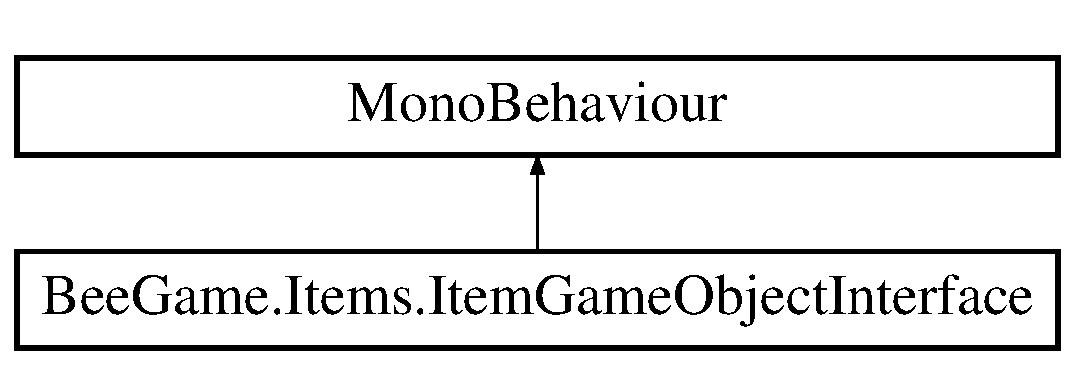
\includegraphics[height=2.000000cm]{class_bee_game_1_1_items_1_1_item_game_object_interface}
\end{center}
\end{figure}
\subsection*{Public Member Functions}
\begin{DoxyCompactItemize}
\item 
void \hyperlink{class_bee_game_1_1_items_1_1_item_game_object_interface_aa88fbff044f2dceb7633b1b41175d085}{Update\+Item\+Data} (\hyperlink{struct_bee_game_1_1_items_1_1_item}{Item} \+\_\+item)
\end{DoxyCompactItemize}
\subsection*{Public Attributes}
\begin{DoxyCompactItemize}
\item 
\hyperlink{struct_bee_game_1_1_items_1_1_item}{Item} \hyperlink{class_bee_game_1_1_items_1_1_item_game_object_interface_abe9476a5393ff778bd99f684b24886ad}{item}
\begin{DoxyCompactList}\small\item\em This interfaces \hyperlink{struct_bee_game_1_1_items_1_1_item}{Item} \end{DoxyCompactList}\end{DoxyCompactItemize}
\subsection*{Private Member Functions}
\begin{DoxyCompactItemize}
\item 
void \hyperlink{class_bee_game_1_1_items_1_1_item_game_object_interface_a1d99080fb7b3b79116ee4638dd4fc127}{Awake} ()
\begin{DoxyCompactList}\small\item\em When this item is made set its position \end{DoxyCompactList}\item 
void \hyperlink{class_bee_game_1_1_items_1_1_item_game_object_interface_a33075cc11237c1f56022d1c380679f27}{Update} ()
\begin{DoxyCompactList}\small\item\em if the item does not have a parent sets it\textquotesingle{}s location to where it is \end{DoxyCompactList}\end{DoxyCompactItemize}


\subsection{Detailed Description}
Interfaces between the \hyperlink{struct_bee_game_1_1_items_1_1_item}{Item} and the Unity Game\+Object as Game\+Object is not serializable with c\# System.\+Runtime.\+Serialization.\+Formatters.\+Binary.\+Binary\+Formatter and neither is Mono\+Behaviour 



Definition at line 11 of file Item\+Game\+Object\+Interface.\+cs.



\subsection{Member Function Documentation}
\mbox{\Hypertarget{class_bee_game_1_1_items_1_1_item_game_object_interface_a1d99080fb7b3b79116ee4638dd4fc127}\label{class_bee_game_1_1_items_1_1_item_game_object_interface_a1d99080fb7b3b79116ee4638dd4fc127}} 
\index{Bee\+Game\+::\+Items\+::\+Item\+Game\+Object\+Interface@{Bee\+Game\+::\+Items\+::\+Item\+Game\+Object\+Interface}!Awake@{Awake}}
\index{Awake@{Awake}!Bee\+Game\+::\+Items\+::\+Item\+Game\+Object\+Interface@{Bee\+Game\+::\+Items\+::\+Item\+Game\+Object\+Interface}}
\subsubsection{\texorpdfstring{Awake()}{Awake()}}
{\footnotesize\ttfamily void Bee\+Game.\+Items.\+Item\+Game\+Object\+Interface.\+Awake (\begin{DoxyParamCaption}{ }\end{DoxyParamCaption})\hspace{0.3cm}{\ttfamily [private]}}



When this item is made set its position 



Definition at line 21 of file Item\+Game\+Object\+Interface.\+cs.


\begin{DoxyCode}
22         \{
23             \textcolor{keywordflow}{if}(\hyperlink{class_bee_game_1_1_items_1_1_item_game_object_interface_abe9476a5393ff778bd99f684b24886ad}{item}.\hyperlink{struct_bee_game_1_1_items_1_1_item_a1343526a0c4c00b82b75513e7852e112}{pos}.\hyperlink{struct_bee_game_1_1_t_h_vector3_a3a414a33eefb779cc52428463f428b6d}{x} != 0)
24             \{
25                 transform.position = \hyperlink{class_bee_game_1_1_items_1_1_item_game_object_interface_abe9476a5393ff778bd99f684b24886ad}{item}.\hyperlink{struct_bee_game_1_1_items_1_1_item_a1343526a0c4c00b82b75513e7852e112}{pos}.ToUnityVector3();
26             \}
27         \}
\end{DoxyCode}
\mbox{\Hypertarget{class_bee_game_1_1_items_1_1_item_game_object_interface_a33075cc11237c1f56022d1c380679f27}\label{class_bee_game_1_1_items_1_1_item_game_object_interface_a33075cc11237c1f56022d1c380679f27}} 
\index{Bee\+Game\+::\+Items\+::\+Item\+Game\+Object\+Interface@{Bee\+Game\+::\+Items\+::\+Item\+Game\+Object\+Interface}!Update@{Update}}
\index{Update@{Update}!Bee\+Game\+::\+Items\+::\+Item\+Game\+Object\+Interface@{Bee\+Game\+::\+Items\+::\+Item\+Game\+Object\+Interface}}
\subsubsection{\texorpdfstring{Update()}{Update()}}
{\footnotesize\ttfamily void Bee\+Game.\+Items.\+Item\+Game\+Object\+Interface.\+Update (\begin{DoxyParamCaption}{ }\end{DoxyParamCaption})\hspace{0.3cm}{\ttfamily [private]}}



if the item does not have a parent sets it\textquotesingle{}s location to where it is 



Definition at line 32 of file Item\+Game\+Object\+Interface.\+cs.


\begin{DoxyCode}
33         \{
34             \textcolor{keywordflow}{if}(transform.parent == null)
35             \{
36                 \hyperlink{class_bee_game_1_1_items_1_1_item_game_object_interface_abe9476a5393ff778bd99f684b24886ad}{item}.\hyperlink{struct_bee_game_1_1_items_1_1_item_a1343526a0c4c00b82b75513e7852e112}{pos} = \textcolor{keyword}{new} THVector3(transform.position);
37             \}
38         \}
\end{DoxyCode}
\mbox{\Hypertarget{class_bee_game_1_1_items_1_1_item_game_object_interface_aa88fbff044f2dceb7633b1b41175d085}\label{class_bee_game_1_1_items_1_1_item_game_object_interface_aa88fbff044f2dceb7633b1b41175d085}} 
\index{Bee\+Game\+::\+Items\+::\+Item\+Game\+Object\+Interface@{Bee\+Game\+::\+Items\+::\+Item\+Game\+Object\+Interface}!Update\+Item\+Data@{Update\+Item\+Data}}
\index{Update\+Item\+Data@{Update\+Item\+Data}!Bee\+Game\+::\+Items\+::\+Item\+Game\+Object\+Interface@{Bee\+Game\+::\+Items\+::\+Item\+Game\+Object\+Interface}}
\subsubsection{\texorpdfstring{Update\+Item\+Data()}{UpdateItemData()}}
{\footnotesize\ttfamily void Bee\+Game.\+Items.\+Item\+Game\+Object\+Interface.\+Update\+Item\+Data (\begin{DoxyParamCaption}\item[{\hyperlink{struct_bee_game_1_1_items_1_1_item}{Item}}]{\+\_\+item }\end{DoxyParamCaption})}



Definition at line 40 of file Item\+Game\+Object\+Interface.\+cs.


\begin{DoxyCode}
41         \{
42             \hyperlink{class_bee_game_1_1_items_1_1_item_game_object_interface_abe9476a5393ff778bd99f684b24886ad}{item} = \_item;
43         \}
\end{DoxyCode}


\subsection{Member Data Documentation}
\mbox{\Hypertarget{class_bee_game_1_1_items_1_1_item_game_object_interface_abe9476a5393ff778bd99f684b24886ad}\label{class_bee_game_1_1_items_1_1_item_game_object_interface_abe9476a5393ff778bd99f684b24886ad}} 
\index{Bee\+Game\+::\+Items\+::\+Item\+Game\+Object\+Interface@{Bee\+Game\+::\+Items\+::\+Item\+Game\+Object\+Interface}!item@{item}}
\index{item@{item}!Bee\+Game\+::\+Items\+::\+Item\+Game\+Object\+Interface@{Bee\+Game\+::\+Items\+::\+Item\+Game\+Object\+Interface}}
\subsubsection{\texorpdfstring{item}{item}}
{\footnotesize\ttfamily \hyperlink{struct_bee_game_1_1_items_1_1_item}{Item} Bee\+Game.\+Items.\+Item\+Game\+Object\+Interface.\+item}



This interfaces \hyperlink{struct_bee_game_1_1_items_1_1_item}{Item} 



Definition at line 16 of file Item\+Game\+Object\+Interface.\+cs.



The documentation for this class was generated from the following file\+:\begin{DoxyCompactItemize}
\item 
C\+:/\+Users/\+Toothless/\+Documents/\+Git\+Hub/\+Bee\+Game/\+Code/\+Bee\+Game/\+Bee\+Game/\+Items/\hyperlink{_item_game_object_interface_8cs}{Item\+Game\+Object\+Interface.\+cs}\end{DoxyCompactItemize}

\hypertarget{class_bee_game_1_1_core_1_1_load_prefabs}{}\section{Bee\+Game.\+Core.\+Load\+Prefabs Class Reference}
\label{class_bee_game_1_1_core_1_1_load_prefabs}\index{Bee\+Game.\+Core.\+Load\+Prefabs@{Bee\+Game.\+Core.\+Load\+Prefabs}}
\subsection*{Static Public Member Functions}
\begin{DoxyCompactItemize}
\item 
static void \hyperlink{class_bee_game_1_1_core_1_1_load_prefabs_ae6045dba0f7f8bad5a1256ff46747614}{Prefab\+Load} ()
\begin{DoxyCompactList}\small\item\em Loads the prefabs from file into prefab dictionary as Game\+Objects \end{DoxyCompactList}\end{DoxyCompactItemize}
\subsection*{Static Private Attributes}
\begin{DoxyCompactItemize}
\item 
static string \hyperlink{class_bee_game_1_1_core_1_1_load_prefabs_a0f61e1d478ea8953fc4cfa5fa4a59b90}{prefab\+Path}
\item 
static string \mbox{[}$\,$\mbox{]} \hyperlink{class_bee_game_1_1_core_1_1_load_prefabs_a774463c4978def7fe0052c4ed1b46549}{split\+Characters} = new string\mbox{[}2\mbox{]} \{ \char`\"{}/\char`\"{}, \char`\"{}.\char`\"{} \}
\end{DoxyCompactItemize}


\subsection{Detailed Description}


Definition at line 7 of file Load\+Prefabs.\+cs.



\subsection{Member Function Documentation}
\mbox{\Hypertarget{class_bee_game_1_1_core_1_1_load_prefabs_ae6045dba0f7f8bad5a1256ff46747614}\label{class_bee_game_1_1_core_1_1_load_prefabs_ae6045dba0f7f8bad5a1256ff46747614}} 
\index{Bee\+Game\+::\+Core\+::\+Load\+Prefabs@{Bee\+Game\+::\+Core\+::\+Load\+Prefabs}!Prefab\+Load@{Prefab\+Load}}
\index{Prefab\+Load@{Prefab\+Load}!Bee\+Game\+::\+Core\+::\+Load\+Prefabs@{Bee\+Game\+::\+Core\+::\+Load\+Prefabs}}
\subsubsection{\texorpdfstring{Prefab\+Load()}{PrefabLoad()}}
{\footnotesize\ttfamily static void Bee\+Game.\+Core.\+Load\+Prefabs.\+Prefab\+Load (\begin{DoxyParamCaption}{ }\end{DoxyParamCaption})\hspace{0.3cm}{\ttfamily [static]}}



Loads the prefabs from file into prefab dictionary as Game\+Objects 



Definition at line 15 of file Load\+Prefabs.\+cs.


\begin{DoxyCode}
16         \{
17             \hyperlink{class_bee_game_1_1_core_1_1_load_prefabs_a0f61e1d478ea8953fc4cfa5fa4a59b90}{prefabPath} = Application.dataPath + \textcolor{stringliteral}{"/Resources/Prefabs/"};
18 
19             \textcolor{comment}{//finds all .prefab files in the directory}
20             \textcolor{keywordflow}{foreach} (\textcolor{keywordtype}{string} s \textcolor{keywordflow}{in} Directory.GetFiles(\hyperlink{class_bee_game_1_1_core_1_1_load_prefabs_a0f61e1d478ea8953fc4cfa5fa4a59b90}{prefabPath}, \textcolor{stringliteral}{"*.prefab"}))
21             \{
22                 \textcolor{keywordtype}{string} prefabName;
23                 \textcolor{keywordtype}{string}[] splitPath;
24 
25                 splitPath = s.Split(\hyperlink{class_bee_game_1_1_core_1_1_load_prefabs_a774463c4978def7fe0052c4ed1b46549}{splitCharacters}, StringSplitOptions.None);
26 
27                 prefabName = splitPath[splitPath.Length - 2];
28 
29                 \textcolor{comment}{//loads found prefab into the profab dictionary}
30                 PrefabDictionary.AddToPrefabDictionary(prefabName, (GameObject)Resources.Load(\textcolor{stringliteral}{"Prefabs/"} + 
      prefabName, typeof(GameObject)));
31             \}
32         \}
\end{DoxyCode}


\subsection{Member Data Documentation}
\mbox{\Hypertarget{class_bee_game_1_1_core_1_1_load_prefabs_a0f61e1d478ea8953fc4cfa5fa4a59b90}\label{class_bee_game_1_1_core_1_1_load_prefabs_a0f61e1d478ea8953fc4cfa5fa4a59b90}} 
\index{Bee\+Game\+::\+Core\+::\+Load\+Prefabs@{Bee\+Game\+::\+Core\+::\+Load\+Prefabs}!prefab\+Path@{prefab\+Path}}
\index{prefab\+Path@{prefab\+Path}!Bee\+Game\+::\+Core\+::\+Load\+Prefabs@{Bee\+Game\+::\+Core\+::\+Load\+Prefabs}}
\subsubsection{\texorpdfstring{prefab\+Path}{prefabPath}}
{\footnotesize\ttfamily string Bee\+Game.\+Core.\+Load\+Prefabs.\+prefab\+Path\hspace{0.3cm}{\ttfamily [static]}, {\ttfamily [private]}}



Definition at line 9 of file Load\+Prefabs.\+cs.

\mbox{\Hypertarget{class_bee_game_1_1_core_1_1_load_prefabs_a774463c4978def7fe0052c4ed1b46549}\label{class_bee_game_1_1_core_1_1_load_prefabs_a774463c4978def7fe0052c4ed1b46549}} 
\index{Bee\+Game\+::\+Core\+::\+Load\+Prefabs@{Bee\+Game\+::\+Core\+::\+Load\+Prefabs}!split\+Characters@{split\+Characters}}
\index{split\+Characters@{split\+Characters}!Bee\+Game\+::\+Core\+::\+Load\+Prefabs@{Bee\+Game\+::\+Core\+::\+Load\+Prefabs}}
\subsubsection{\texorpdfstring{split\+Characters}{splitCharacters}}
{\footnotesize\ttfamily string \mbox{[}$\,$\mbox{]} Bee\+Game.\+Core.\+Load\+Prefabs.\+split\+Characters = new string\mbox{[}2\mbox{]} \{ \char`\"{}/\char`\"{}, \char`\"{}.\char`\"{} \}\hspace{0.3cm}{\ttfamily [static]}, {\ttfamily [private]}}



Definition at line 10 of file Load\+Prefabs.\+cs.



The documentation for this class was generated from the following file\+:\begin{DoxyCompactItemize}
\item 
C\+:/\+Users/\+Toothless/\+Documents/\+Git\+Hub/\+Bee\+Game/\+Code/\+Bee\+Game/\+Bee\+Game/\+Core/\hyperlink{_load_prefabs_8cs}{Load\+Prefabs.\+cs}\end{DoxyCompactItemize}

\hypertarget{class_load_resources}{}\section{Load\+Resources Class Reference}
\label{class_load_resources}\index{Load\+Resources@{Load\+Resources}}
Inheritance diagram for Load\+Resources\+:\begin{figure}[H]
\begin{center}
\leavevmode
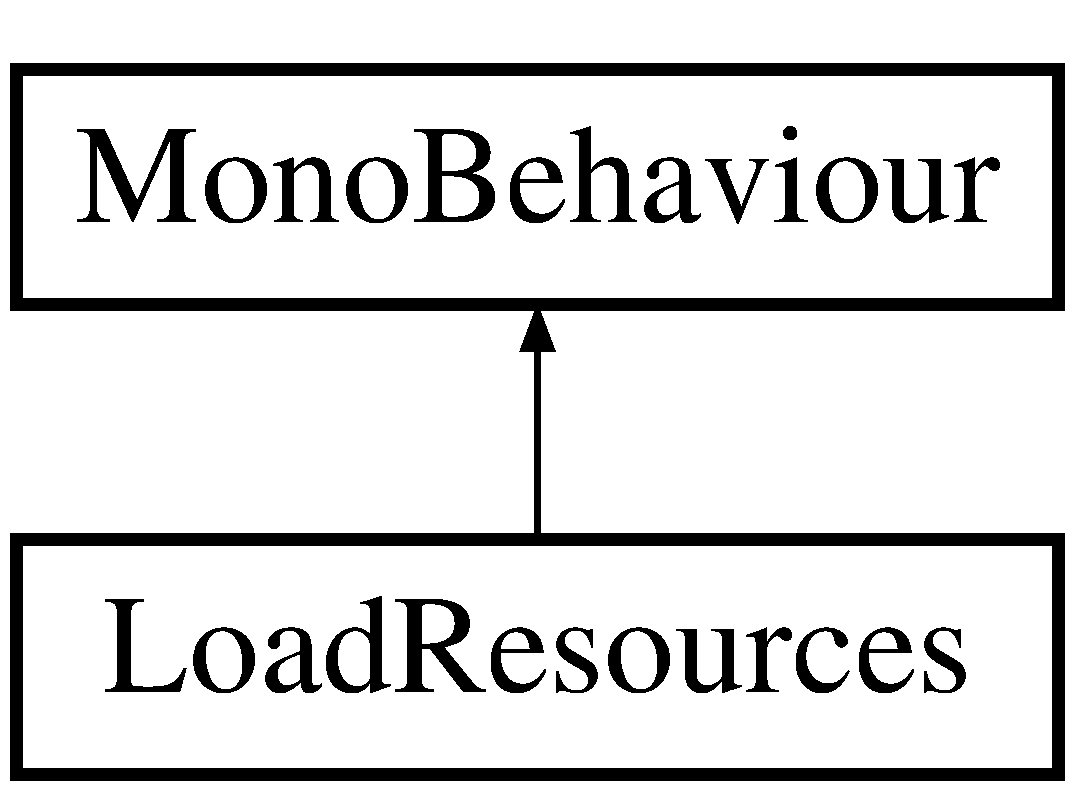
\includegraphics[height=2.000000cm]{class_load_resources}
\end{center}
\end{figure}
\subsection*{Private Member Functions}
\begin{DoxyCompactItemize}
\item 
void \hyperlink{class_load_resources_ac4b32bb35a4c789b1b3fe3b5044001a9}{Start} ()
\item 
void \hyperlink{class_load_resources_a04079f1843cc361e1dc63237af7f24fd}{Fixed\+Update} ()
\end{DoxyCompactItemize}


\subsection{Detailed Description}


Definition at line 5 of file Load\+Resources.\+cs.



\subsection{Member Function Documentation}
\mbox{\Hypertarget{class_load_resources_a04079f1843cc361e1dc63237af7f24fd}\label{class_load_resources_a04079f1843cc361e1dc63237af7f24fd}} 
\index{Load\+Resources@{Load\+Resources}!Fixed\+Update@{Fixed\+Update}}
\index{Fixed\+Update@{Fixed\+Update}!Load\+Resources@{Load\+Resources}}
\subsubsection{\texorpdfstring{Fixed\+Update()}{FixedUpdate()}}
{\footnotesize\ttfamily void Load\+Resources.\+Fixed\+Update (\begin{DoxyParamCaption}{ }\end{DoxyParamCaption})\hspace{0.3cm}{\ttfamily [private]}}



Definition at line 15 of file Load\+Resources.\+cs.


\begin{DoxyCode}
16     \{
17         \hyperlink{class_bee_game_1_1_serialization_1_1_serialization}{Serialization}.\hyperlink{class_bee_game_1_1_serialization_1_1_serialization_ac1a39ee414803d84d970c1d6c03facbc}{Save}();
18     \}
\end{DoxyCode}
\mbox{\Hypertarget{class_load_resources_ac4b32bb35a4c789b1b3fe3b5044001a9}\label{class_load_resources_ac4b32bb35a4c789b1b3fe3b5044001a9}} 
\index{Load\+Resources@{Load\+Resources}!Start@{Start}}
\index{Start@{Start}!Load\+Resources@{Load\+Resources}}
\subsubsection{\texorpdfstring{Start()}{Start()}}
{\footnotesize\ttfamily void Load\+Resources.\+Start (\begin{DoxyParamCaption}{ }\end{DoxyParamCaption})\hspace{0.3cm}{\ttfamily [private]}}



Definition at line 7 of file Load\+Resources.\+cs.


\begin{DoxyCode}
8     \{
9         \hyperlink{class_bee_game_1_1_core_1_1_load_prefabs}{LoadPrefabs}.\hyperlink{class_bee_game_1_1_core_1_1_load_prefabs_ae6045dba0f7f8bad5a1256ff46747614}{PrefabLoad}();
10         \hyperlink{class_bee_game_1_1_core_1_1_load_sprites}{LoadSprites}.\hyperlink{class_bee_game_1_1_core_1_1_load_sprites_a501313d9f5961420d4a9a0ede72f6907}{SpriteLoad}();
11 
12         \hyperlink{class_bee_game_1_1_serialization_1_1_serialization}{Serialization}.\hyperlink{class_bee_game_1_1_serialization_1_1_serialization_a08f39770d6cc2b4a86fd7d7f00ff56a7}{Load}();
13     \}
\end{DoxyCode}


The documentation for this class was generated from the following file\+:\begin{DoxyCompactItemize}
\item 
C\+:/\+Users/\+Toothless/\+Documents/\+Git\+Hub/\+Bee\+Game/\+Code/\+Bee\+Game/\+Bee\+Game/test/\hyperlink{_load_resources_8cs}{Load\+Resources.\+cs}\end{DoxyCompactItemize}

\hypertarget{class_bee_game_1_1_core_1_1_load_sprites}{}\section{Bee\+Game.\+Core.\+Load\+Sprites Class Reference}
\label{class_bee_game_1_1_core_1_1_load_sprites}\index{Bee\+Game.\+Core.\+Load\+Sprites@{Bee\+Game.\+Core.\+Load\+Sprites}}
\subsection*{Static Public Member Functions}
\begin{DoxyCompactItemize}
\item 
static void \hyperlink{class_bee_game_1_1_core_1_1_load_sprites_a501313d9f5961420d4a9a0ede72f6907}{Sprite\+Load} ()
\begin{DoxyCompactList}\small\item\em Loads the sprites in the sprite file into the sprite dictionary \end{DoxyCompactList}\end{DoxyCompactItemize}
\subsection*{Static Private Member Functions}
\begin{DoxyCompactItemize}
\item 
static List$<$ List$<$ string $>$ $>$ \hyperlink{class_bee_game_1_1_core_1_1_load_sprites_a3dca64c0b272b40389047ae9722bfcd3}{Get\+Sprite\+Names} ()
\begin{DoxyCompactList}\small\item\em Looks in the Sprite Names file for the sprite names and filenames \end{DoxyCompactList}\end{DoxyCompactItemize}
\subsection*{Static Private Attributes}
\begin{DoxyCompactItemize}
\item 
static string \mbox{[}$\,$\mbox{]} \hyperlink{class_bee_game_1_1_core_1_1_load_sprites_aaef6cb35c513009a03c13d1307d5bcba}{split\+Characters} = new string\mbox{[}3\mbox{]} \{ \char`\"{}/\char`\"{}, \char`\"{}.\char`\"{}, \char`\"{},\char`\"{}\}
\end{DoxyCompactItemize}


\subsection{Detailed Description}


Definition at line 8 of file Load\+Sprites.\+cs.



\subsection{Member Function Documentation}
\mbox{\Hypertarget{class_bee_game_1_1_core_1_1_load_sprites_a3dca64c0b272b40389047ae9722bfcd3}\label{class_bee_game_1_1_core_1_1_load_sprites_a3dca64c0b272b40389047ae9722bfcd3}} 
\index{Bee\+Game\+::\+Core\+::\+Load\+Sprites@{Bee\+Game\+::\+Core\+::\+Load\+Sprites}!Get\+Sprite\+Names@{Get\+Sprite\+Names}}
\index{Get\+Sprite\+Names@{Get\+Sprite\+Names}!Bee\+Game\+::\+Core\+::\+Load\+Sprites@{Bee\+Game\+::\+Core\+::\+Load\+Sprites}}
\subsubsection{\texorpdfstring{Get\+Sprite\+Names()}{GetSpriteNames()}}
{\footnotesize\ttfamily static List$<$List$<$string$>$ $>$ Bee\+Game.\+Core.\+Load\+Sprites.\+Get\+Sprite\+Names (\begin{DoxyParamCaption}{ }\end{DoxyParamCaption})\hspace{0.3cm}{\ttfamily [static]}, {\ttfamily [private]}}



Looks in the Sprite Names file for the sprite names and filenames 

\begin{DoxyReturn}{Returns}
Sprite Names and File names
\end{DoxyReturn}


Definition at line 29 of file Load\+Sprites.\+cs.


\begin{DoxyCode}
30         \{
31             \textcolor{keywordtype}{string} path = Application.dataPath + \textcolor{stringliteral}{"/Resources/Sprites/SpriteNames.dat"};
32             \textcolor{keywordtype}{string} lineText = \textcolor{stringliteral}{""};
33             List<List<string>> returnSprites = \textcolor{keyword}{new} List<List<string>>();
34 
35             \textcolor{keywordflow}{if}(File.Exists(path))
36             \{
37                 StreamReader objReader;
38                 objReader = \textcolor{keyword}{new} StreamReader(path);
39 
40                 \textcolor{keywordflow}{do}
41                 \{
42                     lineText = objReader.ReadLine();
43                     \textcolor{keywordtype}{string}[] splitSprite = lineText.Split(\hyperlink{class_bee_game_1_1_core_1_1_load_sprites_aaef6cb35c513009a03c13d1307d5bcba}{splitCharacters}, 
      StringSplitOptions.None);
44 
45                     List<string> temp = \textcolor{keyword}{new} List<string>() \{ splitSprite[0], splitSprite[1] \};
46 
47                     returnSprites.Add(temp);
48 
49                 \} \textcolor{keywordflow}{while} (objReader.Peek() != -1);
50 
51                 objReader.Close();
52             \}
53 
54             \textcolor{keywordflow}{return} returnSprites;
55         \}
\end{DoxyCode}
\mbox{\Hypertarget{class_bee_game_1_1_core_1_1_load_sprites_a501313d9f5961420d4a9a0ede72f6907}\label{class_bee_game_1_1_core_1_1_load_sprites_a501313d9f5961420d4a9a0ede72f6907}} 
\index{Bee\+Game\+::\+Core\+::\+Load\+Sprites@{Bee\+Game\+::\+Core\+::\+Load\+Sprites}!Sprite\+Load@{Sprite\+Load}}
\index{Sprite\+Load@{Sprite\+Load}!Bee\+Game\+::\+Core\+::\+Load\+Sprites@{Bee\+Game\+::\+Core\+::\+Load\+Sprites}}
\subsubsection{\texorpdfstring{Sprite\+Load()}{SpriteLoad()}}
{\footnotesize\ttfamily static void Bee\+Game.\+Core.\+Load\+Sprites.\+Sprite\+Load (\begin{DoxyParamCaption}{ }\end{DoxyParamCaption})\hspace{0.3cm}{\ttfamily [static]}}



Loads the sprites in the sprite file into the sprite dictionary 



Definition at line 15 of file Load\+Sprites.\+cs.


\begin{DoxyCode}
16         \{            
17             List<List<string>> sprites = \hyperlink{class_bee_game_1_1_core_1_1_load_sprites_a3dca64c0b272b40389047ae9722bfcd3}{GetSpriteNames}();
18             
19             \textcolor{keywordflow}{for}(\textcolor{keywordtype}{int} i = 0; i < sprites.Count; i++)
20             \{
21                 SpriteDictionary.AddToSpriteDictionary(sprites[i][0], (Sprite)Resources.Load(\textcolor{stringliteral}{"Sprites/"} + 
      sprites[i][1], typeof(Sprite)));
22             \}
23         \}
\end{DoxyCode}


\subsection{Member Data Documentation}
\mbox{\Hypertarget{class_bee_game_1_1_core_1_1_load_sprites_aaef6cb35c513009a03c13d1307d5bcba}\label{class_bee_game_1_1_core_1_1_load_sprites_aaef6cb35c513009a03c13d1307d5bcba}} 
\index{Bee\+Game\+::\+Core\+::\+Load\+Sprites@{Bee\+Game\+::\+Core\+::\+Load\+Sprites}!split\+Characters@{split\+Characters}}
\index{split\+Characters@{split\+Characters}!Bee\+Game\+::\+Core\+::\+Load\+Sprites@{Bee\+Game\+::\+Core\+::\+Load\+Sprites}}
\subsubsection{\texorpdfstring{split\+Characters}{splitCharacters}}
{\footnotesize\ttfamily string \mbox{[}$\,$\mbox{]} Bee\+Game.\+Core.\+Load\+Sprites.\+split\+Characters = new string\mbox{[}3\mbox{]} \{ \char`\"{}/\char`\"{}, \char`\"{}.\char`\"{}, \char`\"{},\char`\"{}\}\hspace{0.3cm}{\ttfamily [static]}, {\ttfamily [private]}}



Definition at line 10 of file Load\+Sprites.\+cs.



The documentation for this class was generated from the following file\+:\begin{DoxyCompactItemize}
\item 
C\+:/\+Users/\+Toothless/\+Documents/\+Git\+Hub/\+Bee\+Game/\+Code/\+Bee\+Game/\+Bee\+Game/\+Core/\hyperlink{_load_sprites_8cs}{Load\+Sprites.\+cs}\end{DoxyCompactItemize}

\hypertarget{class_bee_game_1_1_player_1_1_movement_1_1_move_player}{}\section{Bee\+Game.\+Player.\+Movement.\+Move\+Player Class Reference}
\label{class_bee_game_1_1_player_1_1_movement_1_1_move_player}\index{Bee\+Game.\+Player.\+Movement.\+Move\+Player@{Bee\+Game.\+Player.\+Movement.\+Move\+Player}}
Inheritance diagram for Bee\+Game.\+Player.\+Movement.\+Move\+Player\+:\begin{figure}[H]
\begin{center}
\leavevmode
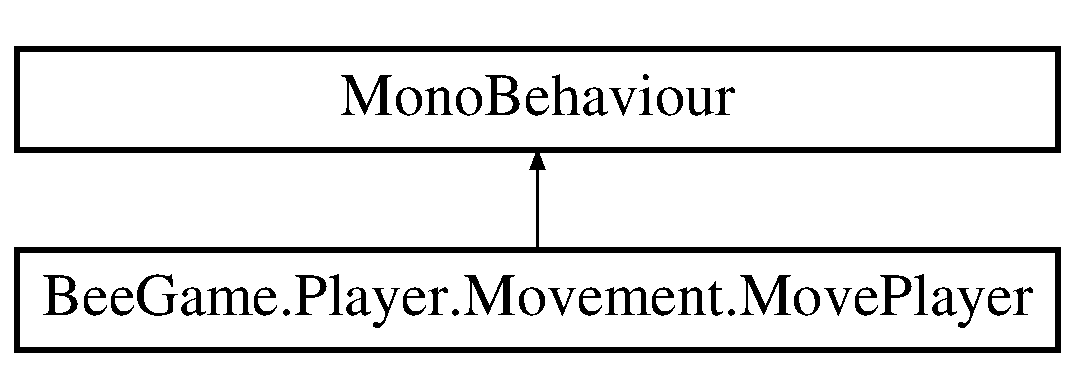
\includegraphics[height=2.000000cm]{class_bee_game_1_1_player_1_1_movement_1_1_move_player}
\end{center}
\end{figure}
\subsection*{Public Attributes}
\begin{DoxyCompactItemize}
\item 
Character\+Controller \hyperlink{class_bee_game_1_1_player_1_1_movement_1_1_move_player_a386e52132d02c2d1c7a2cec66fc223d4}{my\+Conroller}
\item 
float \hyperlink{class_bee_game_1_1_player_1_1_movement_1_1_move_player_a1c75a28f84c06c8d446d3880338ceee8}{speed}
\end{DoxyCompactItemize}
\subsection*{Private Member Functions}
\begin{DoxyCompactItemize}
\item 
void \hyperlink{class_bee_game_1_1_player_1_1_movement_1_1_move_player_af8a97d75b3d79d0773579b8651e2fde2}{Update} ()
\item 
void \hyperlink{class_bee_game_1_1_player_1_1_movement_1_1_move_player_a2ec43ce7923ff96fa77b358f02d1ab37}{Move} ()
\end{DoxyCompactItemize}


\subsection{Detailed Description}


Definition at line 9 of file Move\+Player.\+cs.



\subsection{Member Function Documentation}
\mbox{\Hypertarget{class_bee_game_1_1_player_1_1_movement_1_1_move_player_a2ec43ce7923ff96fa77b358f02d1ab37}\label{class_bee_game_1_1_player_1_1_movement_1_1_move_player_a2ec43ce7923ff96fa77b358f02d1ab37}} 
\index{Bee\+Game\+::\+Player\+::\+Movement\+::\+Move\+Player@{Bee\+Game\+::\+Player\+::\+Movement\+::\+Move\+Player}!Move@{Move}}
\index{Move@{Move}!Bee\+Game\+::\+Player\+::\+Movement\+::\+Move\+Player@{Bee\+Game\+::\+Player\+::\+Movement\+::\+Move\+Player}}
\subsubsection{\texorpdfstring{Move()}{Move()}}
{\footnotesize\ttfamily void Bee\+Game.\+Player.\+Movement.\+Move\+Player.\+Move (\begin{DoxyParamCaption}{ }\end{DoxyParamCaption})\hspace{0.3cm}{\ttfamily [private]}}



Definition at line 19 of file Move\+Player.\+cs.


\begin{DoxyCode}
20         \{
21             \textcolor{keywordflow}{if}(\hyperlink{class_bee_game_1_1_core_1_1_input_manager}{InputManager}.\hyperlink{class_bee_game_1_1_core_1_1_input_manager_a2bd5bb8dc1aaf482f50b9751037eb64c}{GetButton}(\textcolor{stringliteral}{"Forward"}))
22             \{
23                 \hyperlink{class_bee_game_1_1_player_1_1_movement_1_1_move_player_a386e52132d02c2d1c7a2cec66fc223d4}{myConroller}.SimpleMove(transform.forward * \hyperlink{class_bee_game_1_1_player_1_1_movement_1_1_move_player_a1c75a28f84c06c8d446d3880338ceee8}{speed} * Time.deltaTime * Time.
      timeScale);
24             \}
25 
26             \textcolor{keywordflow}{if}(\hyperlink{class_bee_game_1_1_core_1_1_input_manager}{InputManager}.\hyperlink{class_bee_game_1_1_core_1_1_input_manager_a2bd5bb8dc1aaf482f50b9751037eb64c}{GetButton}(\textcolor{stringliteral}{"Backward"}))
27             \{
28                 \hyperlink{class_bee_game_1_1_player_1_1_movement_1_1_move_player_a386e52132d02c2d1c7a2cec66fc223d4}{myConroller}.SimpleMove(transform.forward * -\hyperlink{class_bee_game_1_1_player_1_1_movement_1_1_move_player_a1c75a28f84c06c8d446d3880338ceee8}{speed} * Time.deltaTime * Time.
      timeScale);
29             \}
30 
31             \textcolor{keywordflow}{if}(\hyperlink{class_bee_game_1_1_core_1_1_input_manager}{InputManager}.\hyperlink{class_bee_game_1_1_core_1_1_input_manager_a2bd5bb8dc1aaf482f50b9751037eb64c}{GetButton}(\textcolor{stringliteral}{"Right"}))
32             \{
33                 \hyperlink{class_bee_game_1_1_player_1_1_movement_1_1_move_player_a386e52132d02c2d1c7a2cec66fc223d4}{myConroller}.SimpleMove(transform.right * \hyperlink{class_bee_game_1_1_player_1_1_movement_1_1_move_player_a1c75a28f84c06c8d446d3880338ceee8}{speed} * Time.deltaTime * Time.
      timeScale);
34             \}
35 
36             \textcolor{keywordflow}{if} (\hyperlink{class_bee_game_1_1_core_1_1_input_manager}{InputManager}.\hyperlink{class_bee_game_1_1_core_1_1_input_manager_a2bd5bb8dc1aaf482f50b9751037eb64c}{GetButton}(\textcolor{stringliteral}{"Left"}))
37             \{
38                 \hyperlink{class_bee_game_1_1_player_1_1_movement_1_1_move_player_a386e52132d02c2d1c7a2cec66fc223d4}{myConroller}.SimpleMove(transform.right * -\hyperlink{class_bee_game_1_1_player_1_1_movement_1_1_move_player_a1c75a28f84c06c8d446d3880338ceee8}{speed} * Time.deltaTime * Time.
      timeScale);
39             \}
40         \}
\end{DoxyCode}
\mbox{\Hypertarget{class_bee_game_1_1_player_1_1_movement_1_1_move_player_af8a97d75b3d79d0773579b8651e2fde2}\label{class_bee_game_1_1_player_1_1_movement_1_1_move_player_af8a97d75b3d79d0773579b8651e2fde2}} 
\index{Bee\+Game\+::\+Player\+::\+Movement\+::\+Move\+Player@{Bee\+Game\+::\+Player\+::\+Movement\+::\+Move\+Player}!Update@{Update}}
\index{Update@{Update}!Bee\+Game\+::\+Player\+::\+Movement\+::\+Move\+Player@{Bee\+Game\+::\+Player\+::\+Movement\+::\+Move\+Player}}
\subsubsection{\texorpdfstring{Update()}{Update()}}
{\footnotesize\ttfamily void Bee\+Game.\+Player.\+Movement.\+Move\+Player.\+Update (\begin{DoxyParamCaption}{ }\end{DoxyParamCaption})\hspace{0.3cm}{\ttfamily [private]}}



Definition at line 14 of file Move\+Player.\+cs.


\begin{DoxyCode}
15         \{
16             \hyperlink{class_bee_game_1_1_player_1_1_movement_1_1_move_player_a2ec43ce7923ff96fa77b358f02d1ab37}{Move}();
17         \}
\end{DoxyCode}


\subsection{Member Data Documentation}
\mbox{\Hypertarget{class_bee_game_1_1_player_1_1_movement_1_1_move_player_a386e52132d02c2d1c7a2cec66fc223d4}\label{class_bee_game_1_1_player_1_1_movement_1_1_move_player_a386e52132d02c2d1c7a2cec66fc223d4}} 
\index{Bee\+Game\+::\+Player\+::\+Movement\+::\+Move\+Player@{Bee\+Game\+::\+Player\+::\+Movement\+::\+Move\+Player}!my\+Conroller@{my\+Conroller}}
\index{my\+Conroller@{my\+Conroller}!Bee\+Game\+::\+Player\+::\+Movement\+::\+Move\+Player@{Bee\+Game\+::\+Player\+::\+Movement\+::\+Move\+Player}}
\subsubsection{\texorpdfstring{my\+Conroller}{myConroller}}
{\footnotesize\ttfamily Character\+Controller Bee\+Game.\+Player.\+Movement.\+Move\+Player.\+my\+Conroller}



Definition at line 11 of file Move\+Player.\+cs.

\mbox{\Hypertarget{class_bee_game_1_1_player_1_1_movement_1_1_move_player_a1c75a28f84c06c8d446d3880338ceee8}\label{class_bee_game_1_1_player_1_1_movement_1_1_move_player_a1c75a28f84c06c8d446d3880338ceee8}} 
\index{Bee\+Game\+::\+Player\+::\+Movement\+::\+Move\+Player@{Bee\+Game\+::\+Player\+::\+Movement\+::\+Move\+Player}!speed@{speed}}
\index{speed@{speed}!Bee\+Game\+::\+Player\+::\+Movement\+::\+Move\+Player@{Bee\+Game\+::\+Player\+::\+Movement\+::\+Move\+Player}}
\subsubsection{\texorpdfstring{speed}{speed}}
{\footnotesize\ttfamily float Bee\+Game.\+Player.\+Movement.\+Move\+Player.\+speed}



Definition at line 12 of file Move\+Player.\+cs.



The documentation for this class was generated from the following file\+:\begin{DoxyCompactItemize}
\item 
C\+:/\+Users/\+Toothless/\+Documents/\+Git\+Hub/\+Bee\+Game/\+Code/\+Bee\+Game/\+Bee\+Game/\+Player/\+Movement/\hyperlink{_move_player_8cs}{Move\+Player.\+cs}\end{DoxyCompactItemize}

\hypertarget{class_bee_game_1_1_player_1_1_player_interact}{}\section{Bee\+Game.\+Player.\+Player\+Interact Class Reference}
\label{class_bee_game_1_1_player_1_1_player_interact}\index{Bee\+Game.\+Player.\+Player\+Interact@{Bee\+Game.\+Player.\+Player\+Interact}}
Inheritance diagram for Bee\+Game.\+Player.\+Player\+Interact\+:\begin{figure}[H]
\begin{center}
\leavevmode
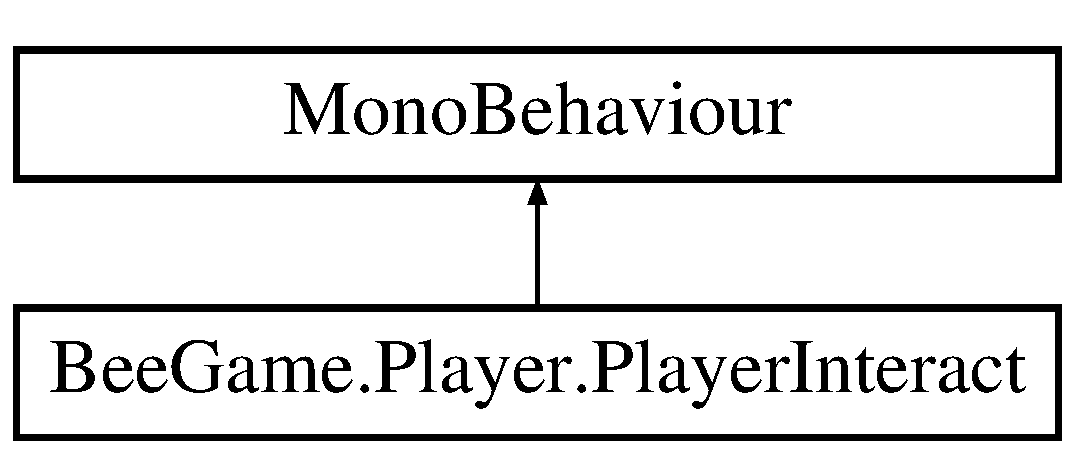
\includegraphics[height=2.000000cm]{class_bee_game_1_1_player_1_1_player_interact}
\end{center}
\end{figure}
\subsection*{Public Attributes}
\begin{DoxyCompactItemize}
\item 
\hyperlink{class_bee_game_1_1_inventory_1_1_player_inventory}{Player\+Inventory} \hyperlink{class_bee_game_1_1_player_1_1_player_interact_af158edc4bacd34c13fffaa1fe4839de2}{player\+Inventory}
\begin{DoxyCompactList}\small\item\em The players inventory \end{DoxyCompactList}\end{DoxyCompactItemize}
\subsection*{Private Member Functions}
\begin{DoxyCompactItemize}
\item 
void \hyperlink{class_bee_game_1_1_player_1_1_player_interact_a8f1c9ab307b82d47066e0d93f27bddbc}{Awake} ()
\begin{DoxyCompactList}\small\item\em Makes a selector and sets it\textquotesingle{}s transform \end{DoxyCompactList}\item 
void \hyperlink{class_bee_game_1_1_player_1_1_player_interact_a795e661cbe900f8a46f8d8667ec43474}{Update} ()
\begin{DoxyCompactList}\small\item\em Every update check for if the user wants to break, place, or interact with a block \end{DoxyCompactList}\item 
void \hyperlink{class_bee_game_1_1_player_1_1_player_interact_a22c84b1a000dbc8775eb9e9d396f26ff}{Update\+Selector} ()
\begin{DoxyCompactList}\small\item\em Updates where the block selector is based on the current look positon \end{DoxyCompactList}\item 
bool \hyperlink{class_bee_game_1_1_player_1_1_player_interact_a47059ea03d8b16b406ed5218c52198a3}{Interact} ()
\begin{DoxyCompactList}\small\item\em Can the player already interact with what is selected \end{DoxyCompactList}\item 
void \hyperlink{class_bee_game_1_1_player_1_1_player_interact_a55ce2fd36c1120aed30893502f1e909f}{Placeblock} ()
\begin{DoxyCompactList}\small\item\em Places a block at the location currently being looked at \end{DoxyCompactList}\item 
bool \hyperlink{class_bee_game_1_1_player_1_1_player_interact_a74a5e5d022edcbc28ab6956cbc8266c8}{Check\+For\+Block} (Vector3 check\+Poz)
\begin{DoxyCompactList}\small\item\em Checks if their is a block already in the position where the new one is supposed to be spawned \end{DoxyCompactList}\item 
void \hyperlink{class_bee_game_1_1_player_1_1_player_interact_a3507c5b70c4aecb332338d518b691875}{Break\+Block} ()
\begin{DoxyCompactList}\small\item\em Breaks the block that the player is looking at \end{DoxyCompactList}\item 
void \hyperlink{class_bee_game_1_1_player_1_1_player_interact_a5e24c97ecd41cfaceaf71d08409d8cca}{Empty\+Block\+Inventory} (Game\+Object \+\_\+game\+Object)
\begin{DoxyCompactList}\small\item\em Emptys the blocks inventory \end{DoxyCompactList}\item 
void \hyperlink{class_bee_game_1_1_player_1_1_player_interact_aacd8f7a70e55d018285ac5f0fd799fd9}{Look\+Poz} ()
\begin{DoxyCompactList}\small\item\em Gets the postion of where the player is looking and sets it to the grid \end{DoxyCompactList}\end{DoxyCompactItemize}
\subsection*{Private Attributes}
\begin{DoxyCompactItemize}
\item 
Game\+Object \hyperlink{class_bee_game_1_1_player_1_1_player_interact_ae6cde5e9d6378a1d750e442fecc9595e}{selector}
\begin{DoxyCompactList}\small\item\em the selector Game\+Object \end{DoxyCompactList}\item 
Raycast\+Hit \hyperlink{class_bee_game_1_1_player_1_1_player_interact_a39537118b4601a3596122f124b684024}{hit}
\begin{DoxyCompactList}\small\item\em What the player is looking at \end{DoxyCompactList}\item 
Vector3 \hyperlink{class_bee_game_1_1_player_1_1_player_interact_ad7b39d8900f206f680945437ff3259a8}{hit\+Alligned}
\begin{DoxyCompactList}\small\item\em The position of the selector alligned to the grid \end{DoxyCompactList}\end{DoxyCompactItemize}


\subsection{Detailed Description}


Definition at line 10 of file Player\+Interact.\+cs.



\subsection{Member Function Documentation}
\mbox{\Hypertarget{class_bee_game_1_1_player_1_1_player_interact_a8f1c9ab307b82d47066e0d93f27bddbc}\label{class_bee_game_1_1_player_1_1_player_interact_a8f1c9ab307b82d47066e0d93f27bddbc}} 
\index{Bee\+Game\+::\+Player\+::\+Player\+Interact@{Bee\+Game\+::\+Player\+::\+Player\+Interact}!Awake@{Awake}}
\index{Awake@{Awake}!Bee\+Game\+::\+Player\+::\+Player\+Interact@{Bee\+Game\+::\+Player\+::\+Player\+Interact}}
\subsubsection{\texorpdfstring{Awake()}{Awake()}}
{\footnotesize\ttfamily void Bee\+Game.\+Player.\+Player\+Interact.\+Awake (\begin{DoxyParamCaption}{ }\end{DoxyParamCaption})\hspace{0.3cm}{\ttfamily [private]}}



Makes a selector and sets it\textquotesingle{}s transform 



Definition at line 32 of file Player\+Interact.\+cs.


\begin{DoxyCode}
33         \{
34             \hyperlink{class_bee_game_1_1_player_1_1_player_interact_ae6cde5e9d6378a1d750e442fecc9595e}{selector} = \hyperlink{class_bee_game_1_1_core_1_1_prefab_dictionary}{PrefabDictionary}.
      \hyperlink{class_bee_game_1_1_core_1_1_prefab_dictionary_a5435ea289663e612fc964438691e32d0}{GetGameObjectItemFromDictionary}(\textcolor{stringliteral}{"Selector"});
35             \hyperlink{class_bee_game_1_1_player_1_1_player_interact_ae6cde5e9d6378a1d750e442fecc9595e}{selector} = Instantiate(\hyperlink{class_bee_game_1_1_player_1_1_player_interact_ae6cde5e9d6378a1d750e442fecc9595e}{selector});
36             \hyperlink{class_bee_game_1_1_player_1_1_player_interact_ae6cde5e9d6378a1d750e442fecc9595e}{selector}.transform.parent = transform;
37         \}
\end{DoxyCode}
\mbox{\Hypertarget{class_bee_game_1_1_player_1_1_player_interact_a3507c5b70c4aecb332338d518b691875}\label{class_bee_game_1_1_player_1_1_player_interact_a3507c5b70c4aecb332338d518b691875}} 
\index{Bee\+Game\+::\+Player\+::\+Player\+Interact@{Bee\+Game\+::\+Player\+::\+Player\+Interact}!Break\+Block@{Break\+Block}}
\index{Break\+Block@{Break\+Block}!Bee\+Game\+::\+Player\+::\+Player\+Interact@{Bee\+Game\+::\+Player\+::\+Player\+Interact}}
\subsubsection{\texorpdfstring{Break\+Block()}{BreakBlock()}}
{\footnotesize\ttfamily void Bee\+Game.\+Player.\+Player\+Interact.\+Break\+Block (\begin{DoxyParamCaption}{ }\end{DoxyParamCaption})\hspace{0.3cm}{\ttfamily [private]}}



Breaks the block that the player is looking at 



Definition at line 136 of file Player\+Interact.\+cs.


\begin{DoxyCode}
137         \{
138             \textcolor{keywordflow}{if}(\hyperlink{class_bee_game_1_1_player_1_1_player_interact_a39537118b4601a3596122f124b684024}{hit}.transform != null)
139             \{
140                 \textcolor{keywordflow}{if} (\hyperlink{class_bee_game_1_1_player_1_1_player_interact_a39537118b4601a3596122f124b684024}{hit}.transform.tag == \textcolor{stringliteral}{"Block"})
141                 \{
142                     \hyperlink{class_bee_game_1_1_serialization_1_1_serialization}{Serialization}.Serialization.
      \hyperlink{class_bee_game_1_1_serialization_1_1_serialization_a248f000bbdc4c3dad2f03018d63fbb9f}{RemoveFromSaveBlocks}(\hyperlink{class_bee_game_1_1_player_1_1_player_interact_a39537118b4601a3596122f124b684024}{hit}.transform.gameObject);
143                     GameObject objectToRemove = \hyperlink{class_bee_game_1_1_player_1_1_player_interact_a39537118b4601a3596122f124b684024}{hit}.collider.gameObject;
144 
145                     \hyperlink{class_bee_game_1_1_player_1_1_player_interact_a5e24c97ecd41cfaceaf71d08409d8cca}{EmptyBlockInventory}(objectToRemove);
146 
147                     \textcolor{keywordflow}{for} (\textcolor{keywordtype}{int} i = objectToRemove.GetComponents<Component>().Length - 1; i >= 4; i--)
148                     \{
149                         Destroy(objectToRemove.GetComponents<Component>()[i]);
150                     \}
151 
152                     objectToRemove.AddComponent<\hyperlink{class_bee_game_1_1_items_1_1_item_game_object_interface}{ItemGameObjectInterface}>();
153                     objectToRemove.GetComponent<\hyperlink{class_bee_game_1_1_items_1_1_item_game_object_interface}{ItemGameObjectInterface}>().
      UpdateItemData(objectToRemove.GetComponent<\hyperlink{class_bee_game_1_1_blocks_1_1_block_game_object_interface}{BlockGameObjectInterface}>().
      \hyperlink{class_bee_game_1_1_blocks_1_1_block_game_object_interface_a224ae292be961a0c3b7675e5a85ddb1b}{ReturnItemData}());
154 
155                     objectToRemove.tag = \textcolor{stringliteral}{"Item"};
156                 \}
157             \}
158         \}
\end{DoxyCode}
\mbox{\Hypertarget{class_bee_game_1_1_player_1_1_player_interact_a74a5e5d022edcbc28ab6956cbc8266c8}\label{class_bee_game_1_1_player_1_1_player_interact_a74a5e5d022edcbc28ab6956cbc8266c8}} 
\index{Bee\+Game\+::\+Player\+::\+Player\+Interact@{Bee\+Game\+::\+Player\+::\+Player\+Interact}!Check\+For\+Block@{Check\+For\+Block}}
\index{Check\+For\+Block@{Check\+For\+Block}!Bee\+Game\+::\+Player\+::\+Player\+Interact@{Bee\+Game\+::\+Player\+::\+Player\+Interact}}
\subsubsection{\texorpdfstring{Check\+For\+Block()}{CheckForBlock()}}
{\footnotesize\ttfamily bool Bee\+Game.\+Player.\+Player\+Interact.\+Check\+For\+Block (\begin{DoxyParamCaption}\item[{Vector3}]{check\+Poz }\end{DoxyParamCaption})\hspace{0.3cm}{\ttfamily [private]}}



Checks if their is a block already in the position where the new one is supposed to be spawned 


\begin{DoxyParams}{Parameters}
{\em check\+Poz} & the Position that sould be checked\\
\hline
\end{DoxyParams}
\begin{DoxyReturn}{Returns}
Returns true if their is a block in the positon
\end{DoxyReturn}


Definition at line 128 of file Player\+Interact.\+cs.


\begin{DoxyCode}
129         \{
130             \textcolor{keywordflow}{return} Physics.CheckSphere(checkPoz, 0.1f);
131         \}
\end{DoxyCode}
\mbox{\Hypertarget{class_bee_game_1_1_player_1_1_player_interact_a5e24c97ecd41cfaceaf71d08409d8cca}\label{class_bee_game_1_1_player_1_1_player_interact_a5e24c97ecd41cfaceaf71d08409d8cca}} 
\index{Bee\+Game\+::\+Player\+::\+Player\+Interact@{Bee\+Game\+::\+Player\+::\+Player\+Interact}!Empty\+Block\+Inventory@{Empty\+Block\+Inventory}}
\index{Empty\+Block\+Inventory@{Empty\+Block\+Inventory}!Bee\+Game\+::\+Player\+::\+Player\+Interact@{Bee\+Game\+::\+Player\+::\+Player\+Interact}}
\subsubsection{\texorpdfstring{Empty\+Block\+Inventory()}{EmptyBlockInventory()}}
{\footnotesize\ttfamily void Bee\+Game.\+Player.\+Player\+Interact.\+Empty\+Block\+Inventory (\begin{DoxyParamCaption}\item[{Game\+Object}]{\+\_\+game\+Object }\end{DoxyParamCaption})\hspace{0.3cm}{\ttfamily [private]}}



Emptys the blocks inventory 


\begin{DoxyParams}{Parameters}
{\em \+\_\+game\+Object} & Gameo\+Object to destroy\\
\hline
\end{DoxyParams}


Definition at line 164 of file Player\+Interact.\+cs.


\begin{DoxyCode}
165         \{
166             \textcolor{keywordflow}{if}(\_gameObject.GetComponent<\hyperlink{class_bee_game_1_1_inventory_1_1_chest_inventory}{ChestInventory}>())
167             \{
168                 \_gameObject.GetComponent<\hyperlink{class_bee_game_1_1_inventory_1_1_chest_inventory}{ChestInventory}>().ChestBroken();
169             \}
170         \}
\end{DoxyCode}
\mbox{\Hypertarget{class_bee_game_1_1_player_1_1_player_interact_a47059ea03d8b16b406ed5218c52198a3}\label{class_bee_game_1_1_player_1_1_player_interact_a47059ea03d8b16b406ed5218c52198a3}} 
\index{Bee\+Game\+::\+Player\+::\+Player\+Interact@{Bee\+Game\+::\+Player\+::\+Player\+Interact}!Interact@{Interact}}
\index{Interact@{Interact}!Bee\+Game\+::\+Player\+::\+Player\+Interact@{Bee\+Game\+::\+Player\+::\+Player\+Interact}}
\subsubsection{\texorpdfstring{Interact()}{Interact()}}
{\footnotesize\ttfamily bool Bee\+Game.\+Player.\+Player\+Interact.\+Interact (\begin{DoxyParamCaption}{ }\end{DoxyParamCaption})\hspace{0.3cm}{\ttfamily [private]}}



Can the player already interact with what is selected 

\begin{DoxyReturn}{Returns}
true if selected object can be interacted with
\end{DoxyReturn}


Definition at line 78 of file Player\+Interact.\+cs.


\begin{DoxyCode}
79         \{
80             \textcolor{keywordflow}{if}(\hyperlink{class_bee_game_1_1_player_1_1_player_interact_a39537118b4601a3596122f124b684024}{hit}.transform != null)
81             \{
82                 \textcolor{keywordflow}{if}(\hyperlink{class_bee_game_1_1_player_1_1_player_interact_a39537118b4601a3596122f124b684024}{hit}.collider.tag == \textcolor{stringliteral}{"Block"})
83                 \{
84                     \textcolor{comment}{// <TODO> Add other interaction scripts here when neccicary}
85                     \textcolor{keywordflow}{if}(\hyperlink{class_bee_game_1_1_player_1_1_player_interact_a39537118b4601a3596122f124b684024}{hit}.collider.GetComponent<\hyperlink{class_bee_game_1_1_inventory_1_1_chest_inventory}{ChestInventory}>())
86                     \{
87                         \hyperlink{class_bee_game_1_1_player_1_1_player_interact_a39537118b4601a3596122f124b684024}{hit}.collider.GetComponent<\hyperlink{class_bee_game_1_1_inventory_1_1_chest_inventory}{ChestInventory}>().OpenChest(
      \hyperlink{class_bee_game_1_1_player_1_1_player_interact_af158edc4bacd34c13fffaa1fe4839de2}{playerInventory});
88                         \textcolor{keywordflow}{return} \textcolor{keyword}{true};
89                     \}
90                     \textcolor{keywordflow}{return} \textcolor{keyword}{false};
91                 \}
92                 \textcolor{keywordflow}{return} \textcolor{keyword}{false};
93             \}
94             \textcolor{keywordflow}{return} \textcolor{keyword}{false};
95         \}
\end{DoxyCode}
\mbox{\Hypertarget{class_bee_game_1_1_player_1_1_player_interact_aacd8f7a70e55d018285ac5f0fd799fd9}\label{class_bee_game_1_1_player_1_1_player_interact_aacd8f7a70e55d018285ac5f0fd799fd9}} 
\index{Bee\+Game\+::\+Player\+::\+Player\+Interact@{Bee\+Game\+::\+Player\+::\+Player\+Interact}!Look\+Poz@{Look\+Poz}}
\index{Look\+Poz@{Look\+Poz}!Bee\+Game\+::\+Player\+::\+Player\+Interact@{Bee\+Game\+::\+Player\+::\+Player\+Interact}}
\subsubsection{\texorpdfstring{Look\+Poz()}{LookPoz()}}
{\footnotesize\ttfamily void Bee\+Game.\+Player.\+Player\+Interact.\+Look\+Poz (\begin{DoxyParamCaption}{ }\end{DoxyParamCaption})\hspace{0.3cm}{\ttfamily [private]}}



Gets the postion of where the player is looking and sets it to the grid 



Definition at line 175 of file Player\+Interact.\+cs.


\begin{DoxyCode}
176         \{
177             Physics.Raycast(transform.position, transform.forward, out \hyperlink{class_bee_game_1_1_player_1_1_player_interact_a39537118b4601a3596122f124b684024}{hit});
178 
179             \textcolor{keywordflow}{if}(hit.transform != null)
180             \{
181                 \textcolor{keywordflow}{if} (hit.collider.tag != \textcolor{stringliteral}{"Block"})
182                 \{
183                     \hyperlink{class_bee_game_1_1_player_1_1_player_interact_ad7b39d8900f206f680945437ff3259a8}{hitAlligned} = \textcolor{keyword}{new} Vector3((\textcolor{keywordtype}{int})hit.point.x, (\textcolor{keywordtype}{int})hit.point.y, (\textcolor{keywordtype}{int})hit.point
      .z);
184                 \}
185                 \textcolor{keywordflow}{else}
186                 \{
187                     \hyperlink{class_bee_game_1_1_player_1_1_player_interact_ad7b39d8900f206f680945437ff3259a8}{hitAlligned} = hit.transform.position;
188                 \}
189             \}
190         \}
\end{DoxyCode}
\mbox{\Hypertarget{class_bee_game_1_1_player_1_1_player_interact_a55ce2fd36c1120aed30893502f1e909f}\label{class_bee_game_1_1_player_1_1_player_interact_a55ce2fd36c1120aed30893502f1e909f}} 
\index{Bee\+Game\+::\+Player\+::\+Player\+Interact@{Bee\+Game\+::\+Player\+::\+Player\+Interact}!Placeblock@{Placeblock}}
\index{Placeblock@{Placeblock}!Bee\+Game\+::\+Player\+::\+Player\+Interact@{Bee\+Game\+::\+Player\+::\+Player\+Interact}}
\subsubsection{\texorpdfstring{Placeblock()}{Placeblock()}}
{\footnotesize\ttfamily void Bee\+Game.\+Player.\+Player\+Interact.\+Placeblock (\begin{DoxyParamCaption}{ }\end{DoxyParamCaption})\hspace{0.3cm}{\ttfamily [private]}}



Places a block at the location currently being looked at 



Definition at line 100 of file Player\+Interact.\+cs.


\begin{DoxyCode}
101         \{
102             \textcolor{keywordflow}{if} (\hyperlink{class_bee_game_1_1_player_1_1_player_interact_af158edc4bacd34c13fffaa1fe4839de2}{playerInventory}.\hyperlink{class_bee_game_1_1_inventory_1_1_player_inventory_a5745fc23291d5916c116500b384bc66e}{ItemPlaceable}())
103             \{
104                 \textcolor{keywordflow}{if} (!\hyperlink{class_bee_game_1_1_player_1_1_player_interact_a74a5e5d022edcbc28ab6956cbc8266c8}{CheckForBlock}((\hyperlink{class_bee_game_1_1_player_1_1_player_interact_ad7b39d8900f206f680945437ff3259a8}{hitAlligned} + \hyperlink{class_bee_game_1_1_player_1_1_player_interact_a39537118b4601a3596122f124b684024}{hit}.normal)))
105                 \{
106                     \textcolor{comment}{//Spawns the GameObject}
107                     GameObject temp = Instantiate(\hyperlink{class_bee_game_1_1_player_1_1_player_interact_af158edc4bacd34c13fffaa1fe4839de2}{playerInventory}.
      \hyperlink{class_bee_game_1_1_inventory_1_1_player_inventory_a30f01639eaee55b92c8feb4a5ab2e5df}{BlockToPlace}(), \hyperlink{class_bee_game_1_1_player_1_1_player_interact_ad7b39d8900f206f680945437ff3259a8}{hitAlligned} + \hyperlink{class_bee_game_1_1_player_1_1_player_interact_a39537118b4601a3596122f124b684024}{hit}.normal, Quaternion.identity);
108                     \textcolor{comment}{//sets the tag}
109                     temp.tag = \textcolor{stringliteral}{"Block"};
110 
111                     Destroy(temp.GetComponent<\hyperlink{class_bee_game_1_1_items_1_1_item_game_object_interface}{ItemGameObjectInterface}>());
112                     temp.AddComponent<\hyperlink{class_bee_game_1_1_blocks_1_1_block_game_object_interface}{BlockGameObjectInterface}>();
113                     temp.GetComponent<\hyperlink{class_bee_game_1_1_blocks_1_1_block_game_object_interface}{BlockGameObjectInterface}>().UpdateBlockData(
      \hyperlink{class_bee_game_1_1_player_1_1_player_interact_af158edc4bacd34c13fffaa1fe4839de2}{playerInventory}.\hyperlink{class_bee_game_1_1_inventory_1_1_player_inventory_a52e75cc8105c299708ac8ccad0d01828}{ItemData}(), \hyperlink{class_bee_game_1_1_core_1_1_extenstion_methods}{ExtenstionMethods}.
      \hyperlink{class_bee_game_1_1_core_1_1_extenstion_methods_a18389aa1c5683971b53d71029ae14a72}{ToTHVecotr3}(temp.transform.position));
114 
115                     \textcolor{comment}{//subtracts from the inventory stack count}
116                     \hyperlink{class_bee_game_1_1_player_1_1_player_interact_af158edc4bacd34c13fffaa1fe4839de2}{playerInventory}.\hyperlink{class_bee_game_1_1_inventory_1_1_player_inventory_ae50a91db412070ff4e43b93c70a4e28d}{RemoveItemFromStack}();
117 
118                     \hyperlink{class_bee_game_1_1_serialization_1_1_serialization}{Serialization}.Serialization.\hyperlink{class_bee_game_1_1_serialization_1_1_serialization_a1cc1b4dcf2acafaa063b5fde22a0dd41}{AddToSaveBlocks}(temp);
119                 \}
120             \}
121         \}
\end{DoxyCode}
\mbox{\Hypertarget{class_bee_game_1_1_player_1_1_player_interact_a795e661cbe900f8a46f8d8667ec43474}\label{class_bee_game_1_1_player_1_1_player_interact_a795e661cbe900f8a46f8d8667ec43474}} 
\index{Bee\+Game\+::\+Player\+::\+Player\+Interact@{Bee\+Game\+::\+Player\+::\+Player\+Interact}!Update@{Update}}
\index{Update@{Update}!Bee\+Game\+::\+Player\+::\+Player\+Interact@{Bee\+Game\+::\+Player\+::\+Player\+Interact}}
\subsubsection{\texorpdfstring{Update()}{Update()}}
{\footnotesize\ttfamily void Bee\+Game.\+Player.\+Player\+Interact.\+Update (\begin{DoxyParamCaption}{ }\end{DoxyParamCaption})\hspace{0.3cm}{\ttfamily [private]}}



Every update check for if the user wants to break, place, or interact with a block 



Definition at line 42 of file Player\+Interact.\+cs.


\begin{DoxyCode}
43         \{
44             \hyperlink{class_bee_game_1_1_player_1_1_player_interact_aacd8f7a70e55d018285ac5f0fd799fd9}{LookPoz}();
45 
46             \hyperlink{class_bee_game_1_1_player_1_1_player_interact_a22c84b1a000dbc8775eb9e9d396f26ff}{UpdateSelector}();
47 
48             \textcolor{keywordflow}{if}(Time.timeScale > 0)
49             \{
50                 \textcolor{keywordflow}{if} (\hyperlink{class_bee_game_1_1_core_1_1_input_manager}{InputManager}.\hyperlink{class_bee_game_1_1_core_1_1_input_manager_ac90aab89652007118b67f60e962103c5}{GetButtonDown}(\textcolor{stringliteral}{"Break Block"}))
51                 \{
52                     \hyperlink{class_bee_game_1_1_player_1_1_player_interact_a3507c5b70c4aecb332338d518b691875}{BreakBlock}();
53                 \}
54 
55                 \textcolor{keywordflow}{if} (\hyperlink{class_bee_game_1_1_core_1_1_input_manager}{InputManager}.\hyperlink{class_bee_game_1_1_core_1_1_input_manager_ac90aab89652007118b67f60e962103c5}{GetButtonDown}(\textcolor{stringliteral}{"Place/Interact"}))
56                 \{
57                     \textcolor{keywordflow}{if} (!\hyperlink{class_bee_game_1_1_player_1_1_player_interact_a47059ea03d8b16b406ed5218c52198a3}{Interact}())
58                     \{
59                         \hyperlink{class_bee_game_1_1_player_1_1_player_interact_a55ce2fd36c1120aed30893502f1e909f}{Placeblock}();
60                     \}
61                 \}
62             \}
63         \}
\end{DoxyCode}
\mbox{\Hypertarget{class_bee_game_1_1_player_1_1_player_interact_a22c84b1a000dbc8775eb9e9d396f26ff}\label{class_bee_game_1_1_player_1_1_player_interact_a22c84b1a000dbc8775eb9e9d396f26ff}} 
\index{Bee\+Game\+::\+Player\+::\+Player\+Interact@{Bee\+Game\+::\+Player\+::\+Player\+Interact}!Update\+Selector@{Update\+Selector}}
\index{Update\+Selector@{Update\+Selector}!Bee\+Game\+::\+Player\+::\+Player\+Interact@{Bee\+Game\+::\+Player\+::\+Player\+Interact}}
\subsubsection{\texorpdfstring{Update\+Selector()}{UpdateSelector()}}
{\footnotesize\ttfamily void Bee\+Game.\+Player.\+Player\+Interact.\+Update\+Selector (\begin{DoxyParamCaption}{ }\end{DoxyParamCaption})\hspace{0.3cm}{\ttfamily [private]}}



Updates where the block selector is based on the current look positon 



Definition at line 68 of file Player\+Interact.\+cs.


\begin{DoxyCode}
69         \{
70             \hyperlink{class_bee_game_1_1_player_1_1_player_interact_ae6cde5e9d6378a1d750e442fecc9595e}{selector}.transform.position = \hyperlink{class_bee_game_1_1_player_1_1_player_interact_ad7b39d8900f206f680945437ff3259a8}{hitAlligned};
71             \hyperlink{class_bee_game_1_1_player_1_1_player_interact_ae6cde5e9d6378a1d750e442fecc9595e}{selector}.transform.rotation = Quaternion.identity;
72         \}
\end{DoxyCode}


\subsection{Member Data Documentation}
\mbox{\Hypertarget{class_bee_game_1_1_player_1_1_player_interact_a39537118b4601a3596122f124b684024}\label{class_bee_game_1_1_player_1_1_player_interact_a39537118b4601a3596122f124b684024}} 
\index{Bee\+Game\+::\+Player\+::\+Player\+Interact@{Bee\+Game\+::\+Player\+::\+Player\+Interact}!hit@{hit}}
\index{hit@{hit}!Bee\+Game\+::\+Player\+::\+Player\+Interact@{Bee\+Game\+::\+Player\+::\+Player\+Interact}}
\subsubsection{\texorpdfstring{hit}{hit}}
{\footnotesize\ttfamily Raycast\+Hit Bee\+Game.\+Player.\+Player\+Interact.\+hit\hspace{0.3cm}{\ttfamily [private]}}



What the player is looking at 



Definition at line 23 of file Player\+Interact.\+cs.

\mbox{\Hypertarget{class_bee_game_1_1_player_1_1_player_interact_ad7b39d8900f206f680945437ff3259a8}\label{class_bee_game_1_1_player_1_1_player_interact_ad7b39d8900f206f680945437ff3259a8}} 
\index{Bee\+Game\+::\+Player\+::\+Player\+Interact@{Bee\+Game\+::\+Player\+::\+Player\+Interact}!hit\+Alligned@{hit\+Alligned}}
\index{hit\+Alligned@{hit\+Alligned}!Bee\+Game\+::\+Player\+::\+Player\+Interact@{Bee\+Game\+::\+Player\+::\+Player\+Interact}}
\subsubsection{\texorpdfstring{hit\+Alligned}{hitAlligned}}
{\footnotesize\ttfamily Vector3 Bee\+Game.\+Player.\+Player\+Interact.\+hit\+Alligned\hspace{0.3cm}{\ttfamily [private]}}



The position of the selector alligned to the grid 



Definition at line 27 of file Player\+Interact.\+cs.

\mbox{\Hypertarget{class_bee_game_1_1_player_1_1_player_interact_af158edc4bacd34c13fffaa1fe4839de2}\label{class_bee_game_1_1_player_1_1_player_interact_af158edc4bacd34c13fffaa1fe4839de2}} 
\index{Bee\+Game\+::\+Player\+::\+Player\+Interact@{Bee\+Game\+::\+Player\+::\+Player\+Interact}!player\+Inventory@{player\+Inventory}}
\index{player\+Inventory@{player\+Inventory}!Bee\+Game\+::\+Player\+::\+Player\+Interact@{Bee\+Game\+::\+Player\+::\+Player\+Interact}}
\subsubsection{\texorpdfstring{player\+Inventory}{playerInventory}}
{\footnotesize\ttfamily \hyperlink{class_bee_game_1_1_inventory_1_1_player_inventory}{Player\+Inventory} Bee\+Game.\+Player.\+Player\+Interact.\+player\+Inventory}



The players inventory 



Definition at line 15 of file Player\+Interact.\+cs.

\mbox{\Hypertarget{class_bee_game_1_1_player_1_1_player_interact_ae6cde5e9d6378a1d750e442fecc9595e}\label{class_bee_game_1_1_player_1_1_player_interact_ae6cde5e9d6378a1d750e442fecc9595e}} 
\index{Bee\+Game\+::\+Player\+::\+Player\+Interact@{Bee\+Game\+::\+Player\+::\+Player\+Interact}!selector@{selector}}
\index{selector@{selector}!Bee\+Game\+::\+Player\+::\+Player\+Interact@{Bee\+Game\+::\+Player\+::\+Player\+Interact}}
\subsubsection{\texorpdfstring{selector}{selector}}
{\footnotesize\ttfamily Game\+Object Bee\+Game.\+Player.\+Player\+Interact.\+selector\hspace{0.3cm}{\ttfamily [private]}}



the selector Game\+Object 



Definition at line 19 of file Player\+Interact.\+cs.



The documentation for this class was generated from the following file\+:\begin{DoxyCompactItemize}
\item 
C\+:/\+Users/\+Toothless/\+Documents/\+Git\+Hub/\+Bee\+Game/\+Code/\+Bee\+Game/\+Bee\+Game/\+Player/\hyperlink{_player_interact_8cs}{Player\+Interact.\+cs}\end{DoxyCompactItemize}

\hypertarget{class_bee_game_1_1_inventory_1_1_player_inventory}{}\section{Bee\+Game.\+Inventory.\+Player\+Inventory Class Reference}
\label{class_bee_game_1_1_inventory_1_1_player_inventory}\index{Bee\+Game.\+Inventory.\+Player\+Inventory@{Bee\+Game.\+Inventory.\+Player\+Inventory}}
Inheritance diagram for Bee\+Game.\+Inventory.\+Player\+Inventory\+:\begin{figure}[H]
\begin{center}
\leavevmode
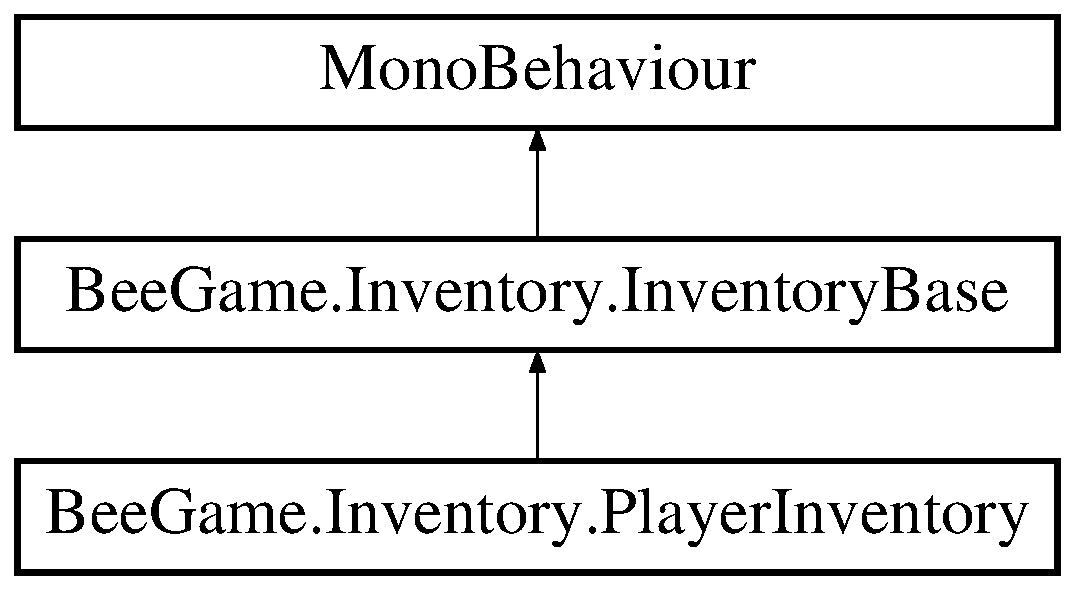
\includegraphics[height=3.000000cm]{class_bee_game_1_1_inventory_1_1_player_inventory}
\end{center}
\end{figure}
\subsection*{Public Member Functions}
\begin{DoxyCompactItemize}
\item 
\hyperlink{struct_bee_game_1_1_items_1_1_item}{Item} \hyperlink{class_bee_game_1_1_inventory_1_1_player_inventory_a52e75cc8105c299708ac8ccad0d01828}{Item\+Data} ()
\begin{DoxyCompactList}\small\item\em the item data that is currently being held \end{DoxyCompactList}\item 
bool \hyperlink{class_bee_game_1_1_inventory_1_1_player_inventory_a5745fc23291d5916c116500b384bc66e}{Item\+Placeable} ()
\begin{DoxyCompactList}\small\item\em Is the item currently selected placeable \end{DoxyCompactList}\item 
Game\+Object \hyperlink{class_bee_game_1_1_inventory_1_1_player_inventory_a30f01639eaee55b92c8feb4a5ab2e5df}{Block\+To\+Place} ()
\begin{DoxyCompactList}\small\item\em Returns the Game\+Object to be instantiated \end{DoxyCompactList}\item 
void \hyperlink{class_bee_game_1_1_inventory_1_1_player_inventory_ae50a91db412070ff4e43b93c70a4e28d}{Remove\+Item\+From\+Stack} ()
\begin{DoxyCompactList}\small\item\em Removes an item from the stack count \end{DoxyCompactList}\item 
void \hyperlink{class_bee_game_1_1_inventory_1_1_player_inventory_a370bc5a57950cdb31f834af4523a8436}{Held\+Player\+Item} (int direction)
\begin{DoxyCompactList}\small\item\em Changes the item currently held by the player \end{DoxyCompactList}\end{DoxyCompactItemize}
\subsection*{Public Attributes}
\begin{DoxyCompactItemize}
\item 
Game\+Object \hyperlink{class_bee_game_1_1_inventory_1_1_player_inventory_a102e6767793ea61ae62dce5840fd405b}{inventory}
\item 
Game\+Object \hyperlink{class_bee_game_1_1_inventory_1_1_player_inventory_a595e1144315e0e9be0b825b538643e1f}{held\+Object\+Inventory}
\begin{DoxyCompactList}\small\item\em The held object inventory(hotbar) of the player \end{DoxyCompactList}\end{DoxyCompactItemize}
\subsection*{Private Member Functions}
\begin{DoxyCompactItemize}
\item 
void \hyperlink{class_bee_game_1_1_inventory_1_1_player_inventory_a3cda67cea8a2cae1ce032a8f0d74912a}{Start} ()
\item 
void \hyperlink{class_bee_game_1_1_inventory_1_1_player_inventory_a340eeb707be60a6ecf909728deaad6c5}{Update} ()
\begin{DoxyCompactList}\small\item\em Will update the players inventory every frame \end{DoxyCompactList}\item 
void \hyperlink{class_bee_game_1_1_inventory_1_1_player_inventory_a1b86d5439ebb9f5dc6d9fefe3351cdc7}{Update\+Hotbar\+Item} ()
\begin{DoxyCompactList}\small\item\em Checks wether the player as selected a dirrerent hotbar item and updates accordingly \end{DoxyCompactList}\item 
void \hyperlink{class_bee_game_1_1_inventory_1_1_player_inventory_a226c92d8b805827199cdd1ed9796a326}{Show\+Hide\+Inventory} ()
\begin{DoxyCompactList}\small\item\em Shows and hides the player inventory \end{DoxyCompactList}\item 
void \hyperlink{class_bee_game_1_1_inventory_1_1_player_inventory_a84caefeadcff40e4fd6e888307a7a1e9}{Pickup\+Item} ()
\begin{DoxyCompactList}\small\item\em Picksup an item on the ground if their is enough space in the inventory \end{DoxyCompactList}\item 
void \hyperlink{class_bee_game_1_1_inventory_1_1_player_inventory_a95bef0a0a994161176a5034fb9bc3444}{Change\+Selected\+Item} (int direction)
\begin{DoxyCompactList}\small\item\em Changes the invenotry slot graphic of the selected slot \end{DoxyCompactList}\item 
void \hyperlink{class_bee_game_1_1_inventory_1_1_player_inventory_a469e47caa8a5bbb4fad1fdd5ec5b4113}{Update\+Held\+Game\+Object} ()
\begin{DoxyCompactList}\small\item\em Updates the object that is currently spawned to represent the object the player is holding \end{DoxyCompactList}\item 
void \hyperlink{class_bee_game_1_1_inventory_1_1_player_inventory_a0e00b423e304507a227ed84df2b6039c}{Spawn\+Object} ()
\begin{DoxyCompactList}\small\item\em Spawns the object that is currently being held by the player \end{DoxyCompactList}\end{DoxyCompactItemize}
\subsection*{Private Attributes}
\begin{DoxyCompactItemize}
\item 
int \hyperlink{class_bee_game_1_1_inventory_1_1_player_inventory_ac2978979c5c8e45fccc7d3a10882ea1b}{current\+Held\+Item\+Index}
\begin{DoxyCompactList}\small\item\em the inventory slot index of the slot the player currently has selected in the hotbar \end{DoxyCompactList}\item 
Game\+Object \hyperlink{class_bee_game_1_1_inventory_1_1_player_inventory_ae30e4d599863e910244ff52ba53a1dfb}{held\+Object}
\begin{DoxyCompactList}\small\item\em The item currently held by the player \end{DoxyCompactList}\item 
int \hyperlink{class_bee_game_1_1_inventory_1_1_player_inventory_a2e16150bcef69b49276c1617d4f2c030}{previous\+Held\+Index}
\end{DoxyCompactItemize}
\subsection*{Additional Inherited Members}


\subsection{Detailed Description}


Definition at line 8 of file Player\+Inventory.\+cs.



\subsection{Member Function Documentation}
\mbox{\Hypertarget{class_bee_game_1_1_inventory_1_1_player_inventory_a30f01639eaee55b92c8feb4a5ab2e5df}\label{class_bee_game_1_1_inventory_1_1_player_inventory_a30f01639eaee55b92c8feb4a5ab2e5df}} 
\index{Bee\+Game\+::\+Inventory\+::\+Player\+Inventory@{Bee\+Game\+::\+Inventory\+::\+Player\+Inventory}!Block\+To\+Place@{Block\+To\+Place}}
\index{Block\+To\+Place@{Block\+To\+Place}!Bee\+Game\+::\+Inventory\+::\+Player\+Inventory@{Bee\+Game\+::\+Inventory\+::\+Player\+Inventory}}
\subsubsection{\texorpdfstring{Block\+To\+Place()}{BlockToPlace()}}
{\footnotesize\ttfamily Game\+Object Bee\+Game.\+Inventory.\+Player\+Inventory.\+Block\+To\+Place (\begin{DoxyParamCaption}{ }\end{DoxyParamCaption})}



Returns the Game\+Object to be instantiated 

\begin{DoxyReturn}{Returns}
Gameobject of the currently selected item
\end{DoxyReturn}


Definition at line 154 of file Player\+Inventory.\+cs.


\begin{DoxyCode}
155         \{
156             \textcolor{keywordflow}{return} \hyperlink{class_bee_game_1_1_inventory_1_1_inventory_base_a48dcba7ad7bfa1bed8c9ae290fb32857}{inventoryGUI}[\hyperlink{class_bee_game_1_1_inventory_1_1_player_inventory_ac2978979c5c8e45fccc7d3a10882ea1b}{currentHeldItemIndex}].
      \hyperlink{class_bee_game_1_1_inventory_1_1_inventory_slot_a31b201e7eef9ed0001a447b3f76a7a81}{item}.\hyperlink{struct_bee_game_1_1_items_1_1_item_af28a8cd4a0eff9d4c18189c5ab525f18}{itemGameobject};
157         \}
\end{DoxyCode}
\mbox{\Hypertarget{class_bee_game_1_1_inventory_1_1_player_inventory_a95bef0a0a994161176a5034fb9bc3444}\label{class_bee_game_1_1_inventory_1_1_player_inventory_a95bef0a0a994161176a5034fb9bc3444}} 
\index{Bee\+Game\+::\+Inventory\+::\+Player\+Inventory@{Bee\+Game\+::\+Inventory\+::\+Player\+Inventory}!Change\+Selected\+Item@{Change\+Selected\+Item}}
\index{Change\+Selected\+Item@{Change\+Selected\+Item}!Bee\+Game\+::\+Inventory\+::\+Player\+Inventory@{Bee\+Game\+::\+Inventory\+::\+Player\+Inventory}}
\subsubsection{\texorpdfstring{Change\+Selected\+Item()}{ChangeSelectedItem()}}
{\footnotesize\ttfamily void Bee\+Game.\+Inventory.\+Player\+Inventory.\+Change\+Selected\+Item (\begin{DoxyParamCaption}\item[{int}]{direction }\end{DoxyParamCaption})\hspace{0.3cm}{\ttfamily [private]}}



Changes the invenotry slot graphic of the selected slot 


\begin{DoxyParams}{Parameters}
{\em direction} & The index of the slot to be selected\\
\hline
\end{DoxyParams}


Definition at line 194 of file Player\+Inventory.\+cs.


\begin{DoxyCode}
195         \{
196             \hyperlink{class_bee_game_1_1_inventory_1_1_inventory_base_a48dcba7ad7bfa1bed8c9ae290fb32857}{inventoryGUI}[\hyperlink{class_bee_game_1_1_inventory_1_1_player_inventory_ac2978979c5c8e45fccc7d3a10882ea1b}{currentHeldItemIndex}].
      \hyperlink{class_bee_game_1_1_inventory_1_1_inventory_slot_abe33997cbde05772253494f20f949483}{UpdateGraphic}();
197             \hyperlink{class_bee_game_1_1_inventory_1_1_inventory_base_a48dcba7ad7bfa1bed8c9ae290fb32857}{inventoryGUI}[\hyperlink{class_bee_game_1_1_inventory_1_1_player_inventory_ac2978979c5c8e45fccc7d3a10882ea1b}{currentHeldItemIndex}].
      \hyperlink{class_bee_game_1_1_inventory_1_1_inventory_slot_adc03a9101c901f82a3dfc778db98cf1f}{UpdateSelectedSlot}(\textcolor{keyword}{false});
198             \hyperlink{class_bee_game_1_1_inventory_1_1_player_inventory_ac2978979c5c8e45fccc7d3a10882ea1b}{currentHeldItemIndex} = direction;
199             \hyperlink{class_bee_game_1_1_inventory_1_1_inventory_base_a48dcba7ad7bfa1bed8c9ae290fb32857}{inventoryGUI}[\hyperlink{class_bee_game_1_1_inventory_1_1_player_inventory_ac2978979c5c8e45fccc7d3a10882ea1b}{currentHeldItemIndex}].
      \hyperlink{class_bee_game_1_1_inventory_1_1_inventory_slot_abe33997cbde05772253494f20f949483}{UpdateGraphic}();
200             \hyperlink{class_bee_game_1_1_inventory_1_1_inventory_base_a48dcba7ad7bfa1bed8c9ae290fb32857}{inventoryGUI}[\hyperlink{class_bee_game_1_1_inventory_1_1_player_inventory_ac2978979c5c8e45fccc7d3a10882ea1b}{currentHeldItemIndex}].
      \hyperlink{class_bee_game_1_1_inventory_1_1_inventory_slot_adc03a9101c901f82a3dfc778db98cf1f}{UpdateSelectedSlot}(\textcolor{keyword}{true});
201         \}
\end{DoxyCode}
\mbox{\Hypertarget{class_bee_game_1_1_inventory_1_1_player_inventory_a370bc5a57950cdb31f834af4523a8436}\label{class_bee_game_1_1_inventory_1_1_player_inventory_a370bc5a57950cdb31f834af4523a8436}} 
\index{Bee\+Game\+::\+Inventory\+::\+Player\+Inventory@{Bee\+Game\+::\+Inventory\+::\+Player\+Inventory}!Held\+Player\+Item@{Held\+Player\+Item}}
\index{Held\+Player\+Item@{Held\+Player\+Item}!Bee\+Game\+::\+Inventory\+::\+Player\+Inventory@{Bee\+Game\+::\+Inventory\+::\+Player\+Inventory}}
\subsubsection{\texorpdfstring{Held\+Player\+Item()}{HeldPlayerItem()}}
{\footnotesize\ttfamily void Bee\+Game.\+Inventory.\+Player\+Inventory.\+Held\+Player\+Item (\begin{DoxyParamCaption}\item[{int}]{direction }\end{DoxyParamCaption})}



Changes the item currently held by the player 


\begin{DoxyParams}{Parameters}
{\em direction} & The direction that the player scrolled in (+ = right, -\/ = left)\\
\hline
\end{DoxyParams}


Definition at line 172 of file Player\+Inventory.\+cs.


\begin{DoxyCode}
173         \{
174             \textcolor{keywordflow}{if} (\hyperlink{class_bee_game_1_1_inventory_1_1_player_inventory_ac2978979c5c8e45fccc7d3a10882ea1b}{currentHeldItemIndex} + direction < inventoryGUI.Length &&
       currentHeldItemIndex + direction > \hyperlink{class_bee_game_1_1_inventory_1_1_inventory_base_a48dcba7ad7bfa1bed8c9ae290fb32857}{inventoryGUI}.Length - 6)
175             \{
176                 \hyperlink{class_bee_game_1_1_inventory_1_1_player_inventory_a95bef0a0a994161176a5034fb9bc3444}{ChangeSelectedItem}(\hyperlink{class_bee_game_1_1_inventory_1_1_player_inventory_ac2978979c5c8e45fccc7d3a10882ea1b}{currentHeldItemIndex} + direction);
177             \}
178             \textcolor{keywordflow}{else} \textcolor{keywordflow}{if} (\hyperlink{class_bee_game_1_1_inventory_1_1_player_inventory_ac2978979c5c8e45fccc7d3a10882ea1b}{currentHeldItemIndex} + direction >= 
      \hyperlink{class_bee_game_1_1_inventory_1_1_inventory_base_a48dcba7ad7bfa1bed8c9ae290fb32857}{inventoryGUI}.Length)
179             \{
180                 \hyperlink{class_bee_game_1_1_inventory_1_1_player_inventory_a95bef0a0a994161176a5034fb9bc3444}{ChangeSelectedItem}(\hyperlink{class_bee_game_1_1_inventory_1_1_inventory_base_a48dcba7ad7bfa1bed8c9ae290fb32857}{inventoryGUI}.Length - 5);
181             \}
182             \textcolor{keywordflow}{else} \textcolor{keywordflow}{if} (\hyperlink{class_bee_game_1_1_inventory_1_1_player_inventory_ac2978979c5c8e45fccc7d3a10882ea1b}{currentHeldItemIndex} + direction < 
      \hyperlink{class_bee_game_1_1_inventory_1_1_inventory_base_a48dcba7ad7bfa1bed8c9ae290fb32857}{inventoryGUI}.Length)
183             \{
184                 \hyperlink{class_bee_game_1_1_inventory_1_1_player_inventory_a95bef0a0a994161176a5034fb9bc3444}{ChangeSelectedItem}(\hyperlink{class_bee_game_1_1_inventory_1_1_inventory_base_a48dcba7ad7bfa1bed8c9ae290fb32857}{inventoryGUI}.Length - 1);
185             \}
186 
187             \hyperlink{class_bee_game_1_1_inventory_1_1_player_inventory_a469e47caa8a5bbb4fad1fdd5ec5b4113}{UpdateHeldGameObject}();
188         \}
\end{DoxyCode}
\mbox{\Hypertarget{class_bee_game_1_1_inventory_1_1_player_inventory_a52e75cc8105c299708ac8ccad0d01828}\label{class_bee_game_1_1_inventory_1_1_player_inventory_a52e75cc8105c299708ac8ccad0d01828}} 
\index{Bee\+Game\+::\+Inventory\+::\+Player\+Inventory@{Bee\+Game\+::\+Inventory\+::\+Player\+Inventory}!Item\+Data@{Item\+Data}}
\index{Item\+Data@{Item\+Data}!Bee\+Game\+::\+Inventory\+::\+Player\+Inventory@{Bee\+Game\+::\+Inventory\+::\+Player\+Inventory}}
\subsubsection{\texorpdfstring{Item\+Data()}{ItemData()}}
{\footnotesize\ttfamily \hyperlink{struct_bee_game_1_1_items_1_1_item}{Item} Bee\+Game.\+Inventory.\+Player\+Inventory.\+Item\+Data (\begin{DoxyParamCaption}{ }\end{DoxyParamCaption})}



the item data that is currently being held 

\begin{DoxyReturn}{Returns}
Return the itm data that is currently being held
\end{DoxyReturn}


Definition at line 136 of file Player\+Inventory.\+cs.


\begin{DoxyCode}
137         \{
138             \textcolor{keywordflow}{return} \hyperlink{class_bee_game_1_1_inventory_1_1_inventory_base_a48dcba7ad7bfa1bed8c9ae290fb32857}{inventoryGUI}[\hyperlink{class_bee_game_1_1_inventory_1_1_player_inventory_ac2978979c5c8e45fccc7d3a10882ea1b}{currentHeldItemIndex}].
      \hyperlink{class_bee_game_1_1_inventory_1_1_inventory_slot_a31b201e7eef9ed0001a447b3f76a7a81}{item};
139         \}
\end{DoxyCode}
\mbox{\Hypertarget{class_bee_game_1_1_inventory_1_1_player_inventory_a5745fc23291d5916c116500b384bc66e}\label{class_bee_game_1_1_inventory_1_1_player_inventory_a5745fc23291d5916c116500b384bc66e}} 
\index{Bee\+Game\+::\+Inventory\+::\+Player\+Inventory@{Bee\+Game\+::\+Inventory\+::\+Player\+Inventory}!Item\+Placeable@{Item\+Placeable}}
\index{Item\+Placeable@{Item\+Placeable}!Bee\+Game\+::\+Inventory\+::\+Player\+Inventory@{Bee\+Game\+::\+Inventory\+::\+Player\+Inventory}}
\subsubsection{\texorpdfstring{Item\+Placeable()}{ItemPlaceable()}}
{\footnotesize\ttfamily bool Bee\+Game.\+Inventory.\+Player\+Inventory.\+Item\+Placeable (\begin{DoxyParamCaption}{ }\end{DoxyParamCaption})}



Is the item currently selected placeable 

\begin{DoxyReturn}{Returns}
true is the item currently held is placeable
\end{DoxyReturn}


Definition at line 146 of file Player\+Inventory.\+cs.


\begin{DoxyCode}
147         \{
148             \textcolor{keywordflow}{return} \hyperlink{class_bee_game_1_1_inventory_1_1_inventory_base_a48dcba7ad7bfa1bed8c9ae290fb32857}{inventoryGUI}[\hyperlink{class_bee_game_1_1_inventory_1_1_player_inventory_ac2978979c5c8e45fccc7d3a10882ea1b}{currentHeldItemIndex}].
      \hyperlink{class_bee_game_1_1_inventory_1_1_inventory_slot_a31b201e7eef9ed0001a447b3f76a7a81}{item}.\hyperlink{struct_bee_game_1_1_items_1_1_item_ae95da57ec69cdb64b656caa5aa42b8c7}{isPlaceable};
149         \}
\end{DoxyCode}
\mbox{\Hypertarget{class_bee_game_1_1_inventory_1_1_player_inventory_a84caefeadcff40e4fd6e888307a7a1e9}\label{class_bee_game_1_1_inventory_1_1_player_inventory_a84caefeadcff40e4fd6e888307a7a1e9}} 
\index{Bee\+Game\+::\+Inventory\+::\+Player\+Inventory@{Bee\+Game\+::\+Inventory\+::\+Player\+Inventory}!Pickup\+Item@{Pickup\+Item}}
\index{Pickup\+Item@{Pickup\+Item}!Bee\+Game\+::\+Inventory\+::\+Player\+Inventory@{Bee\+Game\+::\+Inventory\+::\+Player\+Inventory}}
\subsubsection{\texorpdfstring{Pickup\+Item()}{PickupItem()}}
{\footnotesize\ttfamily void Bee\+Game.\+Inventory.\+Player\+Inventory.\+Pickup\+Item (\begin{DoxyParamCaption}{ }\end{DoxyParamCaption})\hspace{0.3cm}{\ttfamily [private]}}



Picksup an item on the ground if their is enough space in the inventory 



Definition at line 97 of file Player\+Inventory.\+cs.


\begin{DoxyCode}
98         \{
99             RaycastHit[] cols = Physics.SphereCastAll(transform.position, 4f, Vector3.up);
100 
101             \textcolor{keywordflow}{for} (\textcolor{keywordtype}{int} i = 0; i < cols.Length; i++)
102             \{
103                 \textcolor{keywordflow}{if} (cols[i].collider.tag == \textcolor{stringliteral}{"Item"} && cols[i].collider.transform.parent != transform.parent
      )
104                 \{
105                     \hyperlink{struct_bee_game_1_1_items_1_1_item}{Item} item = cols[i].collider.GetComponent<
      \hyperlink{class_bee_game_1_1_items_1_1_item_game_object_interface}{ItemGameObjectInterface}>().item;
106 
107                     \textcolor{keywordflow}{for} (\textcolor{keywordtype}{int} h = 0; h < \hyperlink{class_bee_game_1_1_inventory_1_1_inventory_base_a48dcba7ad7bfa1bed8c9ae290fb32857}{inventoryGUI}.Length; h++)
108                     \{
109                         \textcolor{keywordflow}{if} (\hyperlink{class_bee_game_1_1_inventory_1_1_inventory_base_a48dcba7ad7bfa1bed8c9ae290fb32857}{inventoryGUI}[h].item.\hyperlink{struct_bee_game_1_1_items_1_1_item_aa85bfeab893271c26f8ca41b638ada1c}{itemId} == \textcolor{stringliteral}{""})
110                         \{
111                             \hyperlink{class_bee_game_1_1_inventory_1_1_inventory_base_a48dcba7ad7bfa1bed8c9ae290fb32857}{inventoryGUI}[h].\hyperlink{class_bee_game_1_1_inventory_1_1_inventory_slot_a31b201e7eef9ed0001a447b3f76a7a81}{item} = item;
112                             Destroy(cols[i].collider.gameObject);
113                             \textcolor{keywordflow}{break};
114                         \}
115                         \textcolor{keywordflow}{if} (\hyperlink{class_bee_game_1_1_inventory_1_1_inventory_base_a48dcba7ad7bfa1bed8c9ae290fb32857}{inventoryGUI}[h].item == item)
116                         \{
117                             \textcolor{keywordflow}{if} (\hyperlink{class_bee_game_1_1_inventory_1_1_inventory_base_a48dcba7ad7bfa1bed8c9ae290fb32857}{inventoryGUI}[h].item.\hyperlink{struct_bee_game_1_1_items_1_1_item_a2a58e4a805a560661ce6a4f1f21bfa1d}{isStackable})
118                             \{
119                                 \textcolor{keywordflow}{if} (\hyperlink{class_bee_game_1_1_inventory_1_1_inventory_base_a48dcba7ad7bfa1bed8c9ae290fb32857}{inventoryGUI}[h].item.\hyperlink{struct_bee_game_1_1_items_1_1_item_aaa169917b0e0f8472f20398d5d448388}{stackCount} + item.
      \hyperlink{struct_bee_game_1_1_items_1_1_item_aaa169917b0e0f8472f20398d5d448388}{stackCount} < \hyperlink{class_bee_game_1_1_inventory_1_1_inventory_base_a48dcba7ad7bfa1bed8c9ae290fb32857}{inventoryGUI}[h].\hyperlink{class_bee_game_1_1_inventory_1_1_inventory_slot_a31b201e7eef9ed0001a447b3f76a7a81}{item}.\hyperlink{struct_bee_game_1_1_items_1_1_item_a045f162bbb378f44e8b89af901b29ff3}{maxStackCount} + 1)
120                                 \{
121                                     \hyperlink{class_bee_game_1_1_inventory_1_1_inventory_base_a48dcba7ad7bfa1bed8c9ae290fb32857}{inventoryGUI}[h].\hyperlink{class_bee_game_1_1_inventory_1_1_inventory_slot_a31b201e7eef9ed0001a447b3f76a7a81}{item}.
      \hyperlink{struct_bee_game_1_1_items_1_1_item_aaa169917b0e0f8472f20398d5d448388}{stackCount}++;
122                                     Destroy(cols[i].collider.gameObject);
123                                     \textcolor{keywordflow}{break};
124                                 \}
125                             \}
126                         \}
127                     \}
128                 \}
129             \}
130         \}
\end{DoxyCode}
\mbox{\Hypertarget{class_bee_game_1_1_inventory_1_1_player_inventory_ae50a91db412070ff4e43b93c70a4e28d}\label{class_bee_game_1_1_inventory_1_1_player_inventory_ae50a91db412070ff4e43b93c70a4e28d}} 
\index{Bee\+Game\+::\+Inventory\+::\+Player\+Inventory@{Bee\+Game\+::\+Inventory\+::\+Player\+Inventory}!Remove\+Item\+From\+Stack@{Remove\+Item\+From\+Stack}}
\index{Remove\+Item\+From\+Stack@{Remove\+Item\+From\+Stack}!Bee\+Game\+::\+Inventory\+::\+Player\+Inventory@{Bee\+Game\+::\+Inventory\+::\+Player\+Inventory}}
\subsubsection{\texorpdfstring{Remove\+Item\+From\+Stack()}{RemoveItemFromStack()}}
{\footnotesize\ttfamily void Bee\+Game.\+Inventory.\+Player\+Inventory.\+Remove\+Item\+From\+Stack (\begin{DoxyParamCaption}{ }\end{DoxyParamCaption})}



Removes an item from the stack count 



Definition at line 161 of file Player\+Inventory.\+cs.


\begin{DoxyCode}
162         \{
163             \hyperlink{class_bee_game_1_1_inventory_1_1_inventory_base_a48dcba7ad7bfa1bed8c9ae290fb32857}{inventoryGUI}[\hyperlink{class_bee_game_1_1_inventory_1_1_player_inventory_ac2978979c5c8e45fccc7d3a10882ea1b}{currentHeldItemIndex}].
      \hyperlink{class_bee_game_1_1_inventory_1_1_inventory_slot_a31b201e7eef9ed0001a447b3f76a7a81}{item}.\hyperlink{struct_bee_game_1_1_items_1_1_item_aaa169917b0e0f8472f20398d5d448388}{stackCount} -= 1;
164         \}
\end{DoxyCode}
\mbox{\Hypertarget{class_bee_game_1_1_inventory_1_1_player_inventory_a226c92d8b805827199cdd1ed9796a326}\label{class_bee_game_1_1_inventory_1_1_player_inventory_a226c92d8b805827199cdd1ed9796a326}} 
\index{Bee\+Game\+::\+Inventory\+::\+Player\+Inventory@{Bee\+Game\+::\+Inventory\+::\+Player\+Inventory}!Show\+Hide\+Inventory@{Show\+Hide\+Inventory}}
\index{Show\+Hide\+Inventory@{Show\+Hide\+Inventory}!Bee\+Game\+::\+Inventory\+::\+Player\+Inventory@{Bee\+Game\+::\+Inventory\+::\+Player\+Inventory}}
\subsubsection{\texorpdfstring{Show\+Hide\+Inventory()}{ShowHideInventory()}}
{\footnotesize\ttfamily void Bee\+Game.\+Inventory.\+Player\+Inventory.\+Show\+Hide\+Inventory (\begin{DoxyParamCaption}{ }\end{DoxyParamCaption})\hspace{0.3cm}{\ttfamily [private]}}



Shows and hides the player inventory 



Definition at line 71 of file Player\+Inventory.\+cs.


\begin{DoxyCode}
72         \{
73             \textcolor{keywordflow}{if} (\hyperlink{class_bee_game_1_1_inventory_1_1_player_inventory_a595e1144315e0e9be0b825b538643e1f}{heldObjectInventory}.activeInHierarchy)
74             \{
75                 \textcolor{keywordflow}{if} (\hyperlink{class_bee_game_1_1_core_1_1_input_manager}{InputManager}.\hyperlink{class_bee_game_1_1_core_1_1_input_manager_ac90aab89652007118b67f60e962103c5}{GetButtonDown}(\textcolor{stringliteral}{"Inventory"}))
76                 \{
77                     \hyperlink{class_bee_game_1_1_inventory_1_1_player_inventory_a102e6767793ea61ae62dce5840fd405b}{inventory}.SetActive(!\hyperlink{class_bee_game_1_1_inventory_1_1_player_inventory_a102e6767793ea61ae62dce5840fd405b}{inventory}.activeInHierarchy);
78                     Cursor.visible = !Cursor.visible;
79                 \}
80 
81                 \textcolor{keywordflow}{if} (Cursor.visible)
82                 \{
83                     Time.timeScale = 0;
84                     Cursor.lockState = CursorLockMode.None;
85                 \}
86                 \textcolor{keywordflow}{else}
87                 \{
88                     Time.timeScale = 1;
89                     Cursor.lockState = CursorLockMode.Locked;
90                 \}
91             \}
92         \}
\end{DoxyCode}
\mbox{\Hypertarget{class_bee_game_1_1_inventory_1_1_player_inventory_a0e00b423e304507a227ed84df2b6039c}\label{class_bee_game_1_1_inventory_1_1_player_inventory_a0e00b423e304507a227ed84df2b6039c}} 
\index{Bee\+Game\+::\+Inventory\+::\+Player\+Inventory@{Bee\+Game\+::\+Inventory\+::\+Player\+Inventory}!Spawn\+Object@{Spawn\+Object}}
\index{Spawn\+Object@{Spawn\+Object}!Bee\+Game\+::\+Inventory\+::\+Player\+Inventory@{Bee\+Game\+::\+Inventory\+::\+Player\+Inventory}}
\subsubsection{\texorpdfstring{Spawn\+Object()}{SpawnObject()}}
{\footnotesize\ttfamily void Bee\+Game.\+Inventory.\+Player\+Inventory.\+Spawn\+Object (\begin{DoxyParamCaption}{ }\end{DoxyParamCaption})\hspace{0.3cm}{\ttfamily [private]}}



Spawns the object that is currently being held by the player 



Definition at line 239 of file Player\+Inventory.\+cs.


\begin{DoxyCode}
240         \{
241             \textcolor{keywordflow}{if}(\hyperlink{class_bee_game_1_1_inventory_1_1_inventory_base_a48dcba7ad7bfa1bed8c9ae290fb32857}{inventoryGUI}[\hyperlink{class_bee_game_1_1_inventory_1_1_player_inventory_ac2978979c5c8e45fccc7d3a10882ea1b}{currentHeldItemIndex}].item.itemGameobject)
242             \{
243                 \hyperlink{class_bee_game_1_1_inventory_1_1_player_inventory_ae30e4d599863e910244ff52ba53a1dfb}{heldObject} = Instantiate(\hyperlink{class_bee_game_1_1_inventory_1_1_inventory_base_a48dcba7ad7bfa1bed8c9ae290fb32857}{inventoryGUI}[currentHeldItemIndex].item.
      itemGameobject, transform.position, Quaternion.identity);
244                 \hyperlink{class_bee_game_1_1_inventory_1_1_player_inventory_ae30e4d599863e910244ff52ba53a1dfb}{heldObject}.layer = LayerMask.NameToLayer(\textcolor{stringliteral}{"Ignore Raycast"});
245                 \hyperlink{class_bee_game_1_1_inventory_1_1_player_inventory_ae30e4d599863e910244ff52ba53a1dfb}{heldObject}.tag = \textcolor{stringliteral}{"Player"};
246                 \hyperlink{class_bee_game_1_1_inventory_1_1_player_inventory_ae30e4d599863e910244ff52ba53a1dfb}{heldObject}.transform.localScale = \textcolor{keyword}{new} Vector3(0.1f, 0.1f, 0.1f);
247 
248                 \textcolor{keywordflow}{for} (\textcolor{keywordtype}{int} i = \hyperlink{class_bee_game_1_1_inventory_1_1_player_inventory_ae30e4d599863e910244ff52ba53a1dfb}{heldObject}.GetComponents<Component>().Length - 1; i >= 4; i--)
249                 \{
250                     Destroy(\hyperlink{class_bee_game_1_1_inventory_1_1_player_inventory_ae30e4d599863e910244ff52ba53a1dfb}{heldObject}.GetComponents<Component>()[i]);
251                 \}
252             \}
253         \}
\end{DoxyCode}
\mbox{\Hypertarget{class_bee_game_1_1_inventory_1_1_player_inventory_a3cda67cea8a2cae1ce032a8f0d74912a}\label{class_bee_game_1_1_inventory_1_1_player_inventory_a3cda67cea8a2cae1ce032a8f0d74912a}} 
\index{Bee\+Game\+::\+Inventory\+::\+Player\+Inventory@{Bee\+Game\+::\+Inventory\+::\+Player\+Inventory}!Start@{Start}}
\index{Start@{Start}!Bee\+Game\+::\+Inventory\+::\+Player\+Inventory@{Bee\+Game\+::\+Inventory\+::\+Player\+Inventory}}
\subsubsection{\texorpdfstring{Start()}{Start()}}
{\footnotesize\ttfamily void Bee\+Game.\+Inventory.\+Player\+Inventory.\+Start (\begin{DoxyParamCaption}{ }\end{DoxyParamCaption})\hspace{0.3cm}{\ttfamily [private]}}



Definition at line 30 of file Player\+Inventory.\+cs.


\begin{DoxyCode}
31         \{
32             \hyperlink{class_bee_game_1_1_inventory_1_1_player_inventory_a595e1144315e0e9be0b825b538643e1f}{heldObjectInventory} = GameObject.Find(\textcolor{stringliteral}{"Inventory"});
33             \hyperlink{class_bee_game_1_1_inventory_1_1_player_inventory_ac2978979c5c8e45fccc7d3a10882ea1b}{currentHeldItemIndex} = \hyperlink{class_bee_game_1_1_inventory_1_1_inventory_base_a48dcba7ad7bfa1bed8c9ae290fb32857}{inventoryGUI}.Length - 5;
34             \hyperlink{class_bee_game_1_1_inventory_1_1_inventory_base_a48dcba7ad7bfa1bed8c9ae290fb32857}{inventoryGUI}[\hyperlink{class_bee_game_1_1_inventory_1_1_player_inventory_ac2978979c5c8e45fccc7d3a10882ea1b}{currentHeldItemIndex}].
      \hyperlink{class_bee_game_1_1_inventory_1_1_inventory_slot_adc03a9101c901f82a3dfc778db98cf1f}{UpdateSelectedSlot}(\textcolor{keyword}{true});
35         \}
\end{DoxyCode}
\mbox{\Hypertarget{class_bee_game_1_1_inventory_1_1_player_inventory_a340eeb707be60a6ecf909728deaad6c5}\label{class_bee_game_1_1_inventory_1_1_player_inventory_a340eeb707be60a6ecf909728deaad6c5}} 
\index{Bee\+Game\+::\+Inventory\+::\+Player\+Inventory@{Bee\+Game\+::\+Inventory\+::\+Player\+Inventory}!Update@{Update}}
\index{Update@{Update}!Bee\+Game\+::\+Inventory\+::\+Player\+Inventory@{Bee\+Game\+::\+Inventory\+::\+Player\+Inventory}}
\subsubsection{\texorpdfstring{Update()}{Update()}}
{\footnotesize\ttfamily void Bee\+Game.\+Inventory.\+Player\+Inventory.\+Update (\begin{DoxyParamCaption}{ }\end{DoxyParamCaption})\hspace{0.3cm}{\ttfamily [private]}}



Will update the players inventory every frame 



Definition at line 40 of file Player\+Inventory.\+cs.


\begin{DoxyCode}
41         \{
42             \hyperlink{class_bee_game_1_1_inventory_1_1_inventory_base_aa1a965cf7ba9e04b22a4ef85ad133854}{UpdateBase}();
43             \hyperlink{class_bee_game_1_1_inventory_1_1_player_inventory_a1b86d5439ebb9f5dc6d9fefe3351cdc7}{UpdateHotbarItem}();
44             \hyperlink{class_bee_game_1_1_inventory_1_1_player_inventory_a84caefeadcff40e4fd6e888307a7a1e9}{PickupItem}();
45             \hyperlink{class_bee_game_1_1_inventory_1_1_player_inventory_a226c92d8b805827199cdd1ed9796a326}{ShowHideInventory}();
46             
47             \hyperlink{class_bee_game_1_1_inventory_1_1_player_inventory_a469e47caa8a5bbb4fad1fdd5ec5b4113}{UpdateHeldGameObject}();
48         \}
\end{DoxyCode}
\mbox{\Hypertarget{class_bee_game_1_1_inventory_1_1_player_inventory_a469e47caa8a5bbb4fad1fdd5ec5b4113}\label{class_bee_game_1_1_inventory_1_1_player_inventory_a469e47caa8a5bbb4fad1fdd5ec5b4113}} 
\index{Bee\+Game\+::\+Inventory\+::\+Player\+Inventory@{Bee\+Game\+::\+Inventory\+::\+Player\+Inventory}!Update\+Held\+Game\+Object@{Update\+Held\+Game\+Object}}
\index{Update\+Held\+Game\+Object@{Update\+Held\+Game\+Object}!Bee\+Game\+::\+Inventory\+::\+Player\+Inventory@{Bee\+Game\+::\+Inventory\+::\+Player\+Inventory}}
\subsubsection{\texorpdfstring{Update\+Held\+Game\+Object()}{UpdateHeldGameObject()}}
{\footnotesize\ttfamily void Bee\+Game.\+Inventory.\+Player\+Inventory.\+Update\+Held\+Game\+Object (\begin{DoxyParamCaption}{ }\end{DoxyParamCaption})\hspace{0.3cm}{\ttfamily [private]}}



Updates the object that is currently spawned to represent the object the player is holding 



Definition at line 209 of file Player\+Inventory.\+cs.


\begin{DoxyCode}
210         \{
211             \textcolor{keywordflow}{if}(\hyperlink{class_bee_game_1_1_inventory_1_1_player_inventory_ae30e4d599863e910244ff52ba53a1dfb}{heldObject} == null && (\hyperlink{class_bee_game_1_1_inventory_1_1_player_inventory_a2e16150bcef69b49276c1617d4f2c030}{previousHeldIndex} != 
      \hyperlink{class_bee_game_1_1_inventory_1_1_player_inventory_ac2978979c5c8e45fccc7d3a10882ea1b}{currentHeldItemIndex}))
212             \{
213                 \textcolor{keywordflow}{if}(\hyperlink{class_bee_game_1_1_inventory_1_1_inventory_base_a48dcba7ad7bfa1bed8c9ae290fb32857}{inventoryGUI}[\hyperlink{class_bee_game_1_1_inventory_1_1_player_inventory_ac2978979c5c8e45fccc7d3a10882ea1b}{currentHeldItemIndex}].item.itemId != null)
214                 \{
215                     \hyperlink{class_bee_game_1_1_inventory_1_1_player_inventory_a2e16150bcef69b49276c1617d4f2c030}{previousHeldIndex} = \hyperlink{class_bee_game_1_1_inventory_1_1_player_inventory_ac2978979c5c8e45fccc7d3a10882ea1b}{currentHeldItemIndex};
216                     \hyperlink{class_bee_game_1_1_inventory_1_1_player_inventory_a0e00b423e304507a227ed84df2b6039c}{SpawnObject}();
217                 \}
218             \}
219             \textcolor{keywordflow}{else} \textcolor{keywordflow}{if}(\hyperlink{class_bee_game_1_1_inventory_1_1_player_inventory_a2e16150bcef69b49276c1617d4f2c030}{previousHeldIndex} != \hyperlink{class_bee_game_1_1_inventory_1_1_player_inventory_ac2978979c5c8e45fccc7d3a10882ea1b}{currentHeldItemIndex})
220             \{
221                 Destroy(\hyperlink{class_bee_game_1_1_inventory_1_1_player_inventory_ae30e4d599863e910244ff52ba53a1dfb}{heldObject});
222                 \hyperlink{class_bee_game_1_1_inventory_1_1_player_inventory_a2e16150bcef69b49276c1617d4f2c030}{previousHeldIndex} = \hyperlink{class_bee_game_1_1_inventory_1_1_player_inventory_ac2978979c5c8e45fccc7d3a10882ea1b}{currentHeldItemIndex};
223 
224                 \textcolor{keywordflow}{if} (\hyperlink{class_bee_game_1_1_inventory_1_1_inventory_base_a48dcba7ad7bfa1bed8c9ae290fb32857}{inventoryGUI}[\hyperlink{class_bee_game_1_1_inventory_1_1_player_inventory_ac2978979c5c8e45fccc7d3a10882ea1b}{currentHeldItemIndex}].item.itemId != null)
225                 \{
226                     \hyperlink{class_bee_game_1_1_inventory_1_1_player_inventory_a0e00b423e304507a227ed84df2b6039c}{SpawnObject}();
227                 \}
228             \}
229             \textcolor{keywordflow}{else} \textcolor{keywordflow}{if}(\hyperlink{class_bee_game_1_1_inventory_1_1_player_inventory_ae30e4d599863e910244ff52ba53a1dfb}{heldObject} != null && \hyperlink{class_bee_game_1_1_inventory_1_1_inventory_base_a48dcba7ad7bfa1bed8c9ae290fb32857}{inventoryGUI}[
      \hyperlink{class_bee_game_1_1_inventory_1_1_player_inventory_ac2978979c5c8e45fccc7d3a10882ea1b}{currentHeldItemIndex}].item.itemId == null)
230             \{
231                 Destroy(\hyperlink{class_bee_game_1_1_inventory_1_1_player_inventory_ae30e4d599863e910244ff52ba53a1dfb}{heldObject});
232                 \hyperlink{class_bee_game_1_1_inventory_1_1_player_inventory_a2e16150bcef69b49276c1617d4f2c030}{previousHeldIndex} = \hyperlink{class_bee_game_1_1_inventory_1_1_player_inventory_ac2978979c5c8e45fccc7d3a10882ea1b}{currentHeldItemIndex};
233             \}
234         \}
\end{DoxyCode}
\mbox{\Hypertarget{class_bee_game_1_1_inventory_1_1_player_inventory_a1b86d5439ebb9f5dc6d9fefe3351cdc7}\label{class_bee_game_1_1_inventory_1_1_player_inventory_a1b86d5439ebb9f5dc6d9fefe3351cdc7}} 
\index{Bee\+Game\+::\+Inventory\+::\+Player\+Inventory@{Bee\+Game\+::\+Inventory\+::\+Player\+Inventory}!Update\+Hotbar\+Item@{Update\+Hotbar\+Item}}
\index{Update\+Hotbar\+Item@{Update\+Hotbar\+Item}!Bee\+Game\+::\+Inventory\+::\+Player\+Inventory@{Bee\+Game\+::\+Inventory\+::\+Player\+Inventory}}
\subsubsection{\texorpdfstring{Update\+Hotbar\+Item()}{UpdateHotbarItem()}}
{\footnotesize\ttfamily void Bee\+Game.\+Inventory.\+Player\+Inventory.\+Update\+Hotbar\+Item (\begin{DoxyParamCaption}{ }\end{DoxyParamCaption})\hspace{0.3cm}{\ttfamily [private]}}



Checks wether the player as selected a dirrerent hotbar item and updates accordingly 



Definition at line 53 of file Player\+Inventory.\+cs.


\begin{DoxyCode}
54         \{
55             \textcolor{keywordflow}{if} (Time.timeScale > 0)
56             \{
57                 \textcolor{keywordflow}{if} (Input.GetAxis(\textcolor{stringliteral}{"Mouse ScrollWheel"}) > 0)
58                 \{
59                     \hyperlink{class_bee_game_1_1_inventory_1_1_player_inventory_a370bc5a57950cdb31f834af4523a8436}{HeldPlayerItem}(1);
60                 \}
61                 \textcolor{keywordflow}{else} \textcolor{keywordflow}{if} (Input.GetAxis(\textcolor{stringliteral}{"Mouse ScrollWheel"}) < 0)
62                 \{
63                     \hyperlink{class_bee_game_1_1_inventory_1_1_player_inventory_a370bc5a57950cdb31f834af4523a8436}{HeldPlayerItem}(-1);
64                 \}
65             \}
66         \}
\end{DoxyCode}


\subsection{Member Data Documentation}
\mbox{\Hypertarget{class_bee_game_1_1_inventory_1_1_player_inventory_ac2978979c5c8e45fccc7d3a10882ea1b}\label{class_bee_game_1_1_inventory_1_1_player_inventory_ac2978979c5c8e45fccc7d3a10882ea1b}} 
\index{Bee\+Game\+::\+Inventory\+::\+Player\+Inventory@{Bee\+Game\+::\+Inventory\+::\+Player\+Inventory}!current\+Held\+Item\+Index@{current\+Held\+Item\+Index}}
\index{current\+Held\+Item\+Index@{current\+Held\+Item\+Index}!Bee\+Game\+::\+Inventory\+::\+Player\+Inventory@{Bee\+Game\+::\+Inventory\+::\+Player\+Inventory}}
\subsubsection{\texorpdfstring{current\+Held\+Item\+Index}{currentHeldItemIndex}}
{\footnotesize\ttfamily int Bee\+Game.\+Inventory.\+Player\+Inventory.\+current\+Held\+Item\+Index\hspace{0.3cm}{\ttfamily [private]}}



the inventory slot index of the slot the player currently has selected in the hotbar 



Definition at line 22 of file Player\+Inventory.\+cs.

\mbox{\Hypertarget{class_bee_game_1_1_inventory_1_1_player_inventory_ae30e4d599863e910244ff52ba53a1dfb}\label{class_bee_game_1_1_inventory_1_1_player_inventory_ae30e4d599863e910244ff52ba53a1dfb}} 
\index{Bee\+Game\+::\+Inventory\+::\+Player\+Inventory@{Bee\+Game\+::\+Inventory\+::\+Player\+Inventory}!held\+Object@{held\+Object}}
\index{held\+Object@{held\+Object}!Bee\+Game\+::\+Inventory\+::\+Player\+Inventory@{Bee\+Game\+::\+Inventory\+::\+Player\+Inventory}}
\subsubsection{\texorpdfstring{held\+Object}{heldObject}}
{\footnotesize\ttfamily Game\+Object Bee\+Game.\+Inventory.\+Player\+Inventory.\+held\+Object\hspace{0.3cm}{\ttfamily [private]}}



The item currently held by the player 



Definition at line 28 of file Player\+Inventory.\+cs.

\mbox{\Hypertarget{class_bee_game_1_1_inventory_1_1_player_inventory_a595e1144315e0e9be0b825b538643e1f}\label{class_bee_game_1_1_inventory_1_1_player_inventory_a595e1144315e0e9be0b825b538643e1f}} 
\index{Bee\+Game\+::\+Inventory\+::\+Player\+Inventory@{Bee\+Game\+::\+Inventory\+::\+Player\+Inventory}!held\+Object\+Inventory@{held\+Object\+Inventory}}
\index{held\+Object\+Inventory@{held\+Object\+Inventory}!Bee\+Game\+::\+Inventory\+::\+Player\+Inventory@{Bee\+Game\+::\+Inventory\+::\+Player\+Inventory}}
\subsubsection{\texorpdfstring{held\+Object\+Inventory}{heldObjectInventory}}
{\footnotesize\ttfamily Game\+Object Bee\+Game.\+Inventory.\+Player\+Inventory.\+held\+Object\+Inventory}



The held object inventory(hotbar) of the player 



Definition at line 16 of file Player\+Inventory.\+cs.

\mbox{\Hypertarget{class_bee_game_1_1_inventory_1_1_player_inventory_a102e6767793ea61ae62dce5840fd405b}\label{class_bee_game_1_1_inventory_1_1_player_inventory_a102e6767793ea61ae62dce5840fd405b}} 
\index{Bee\+Game\+::\+Inventory\+::\+Player\+Inventory@{Bee\+Game\+::\+Inventory\+::\+Player\+Inventory}!inventory@{inventory}}
\index{inventory@{inventory}!Bee\+Game\+::\+Inventory\+::\+Player\+Inventory@{Bee\+Game\+::\+Inventory\+::\+Player\+Inventory}}
\subsubsection{\texorpdfstring{inventory}{inventory}}
{\footnotesize\ttfamily Game\+Object Bee\+Game.\+Inventory.\+Player\+Inventory.\+inventory}



Definition at line 10 of file Player\+Inventory.\+cs.

\mbox{\Hypertarget{class_bee_game_1_1_inventory_1_1_player_inventory_a2e16150bcef69b49276c1617d4f2c030}\label{class_bee_game_1_1_inventory_1_1_player_inventory_a2e16150bcef69b49276c1617d4f2c030}} 
\index{Bee\+Game\+::\+Inventory\+::\+Player\+Inventory@{Bee\+Game\+::\+Inventory\+::\+Player\+Inventory}!previous\+Held\+Index@{previous\+Held\+Index}}
\index{previous\+Held\+Index@{previous\+Held\+Index}!Bee\+Game\+::\+Inventory\+::\+Player\+Inventory@{Bee\+Game\+::\+Inventory\+::\+Player\+Inventory}}
\subsubsection{\texorpdfstring{previous\+Held\+Index}{previousHeldIndex}}
{\footnotesize\ttfamily int Bee\+Game.\+Inventory.\+Player\+Inventory.\+previous\+Held\+Index\hspace{0.3cm}{\ttfamily [private]}}



Definition at line 205 of file Player\+Inventory.\+cs.



The documentation for this class was generated from the following file\+:\begin{DoxyCompactItemize}
\item 
C\+:/\+Users/\+Toothless/\+Documents/\+Git\+Hub/\+Bee\+Game/\+Code/\+Bee\+Game/\+Bee\+Game/\+Inventory/\hyperlink{_player_inventory_8cs}{Player\+Inventory.\+cs}\end{DoxyCompactItemize}

\hypertarget{class_bee_game_1_1_player_1_1_movement_1_1_player_look}{}\section{Bee\+Game.\+Player.\+Movement.\+Player\+Look Class Reference}
\label{class_bee_game_1_1_player_1_1_movement_1_1_player_look}\index{Bee\+Game.\+Player.\+Movement.\+Player\+Look@{Bee\+Game.\+Player.\+Movement.\+Player\+Look}}
Inheritance diagram for Bee\+Game.\+Player.\+Movement.\+Player\+Look\+:\begin{figure}[H]
\begin{center}
\leavevmode
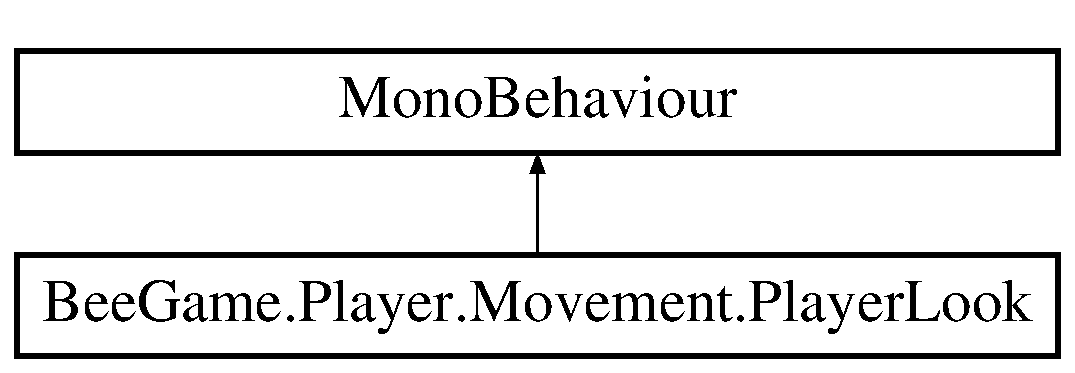
\includegraphics[height=2.000000cm]{class_bee_game_1_1_player_1_1_movement_1_1_player_look}
\end{center}
\end{figure}
\subsection*{Public Attributes}
\begin{DoxyCompactItemize}
\item 
Transform \hyperlink{class_bee_game_1_1_player_1_1_movement_1_1_player_look_a1b69a0e4304df8fa02e0de3e01b6496b}{my\+Transform}
\item 
float \hyperlink{class_bee_game_1_1_player_1_1_movement_1_1_player_look_a3f8df80729aadaeec0471cf881ff608b}{rotation\+Lock}
\item 
float \hyperlink{class_bee_game_1_1_player_1_1_movement_1_1_player_look_ac3a467fcbf2ab53ee216168c51a1349e}{speed} = 5
\end{DoxyCompactItemize}
\subsection*{Private Member Functions}
\begin{DoxyCompactItemize}
\item 
void \hyperlink{class_bee_game_1_1_player_1_1_movement_1_1_player_look_aab0cc79656034e470e212ef2250837f8}{Start} ()
\item 
void \hyperlink{class_bee_game_1_1_player_1_1_movement_1_1_player_look_a6c3528a5b241f1169b8c5584401bbed2}{Update} ()
\item 
void \hyperlink{class_bee_game_1_1_player_1_1_movement_1_1_player_look_a7ff4392d11c1a3c25b80a207de1b5536}{Look} ()
\end{DoxyCompactItemize}
\subsection*{Private Attributes}
\begin{DoxyCompactItemize}
\item 
float \hyperlink{class_bee_game_1_1_player_1_1_movement_1_1_player_look_a3eb9d7e0aad01bed50a29e2ae00b24d6}{y\+Rot} = 0
\item 
float \hyperlink{class_bee_game_1_1_player_1_1_movement_1_1_player_look_a1a939bae4cc533cc5bb4ad9aa6a5bd91}{x\+Rot} = 0
\end{DoxyCompactItemize}


\subsection{Detailed Description}


Definition at line 8 of file Player\+Look.\+cs.



\subsection{Member Function Documentation}
\mbox{\Hypertarget{class_bee_game_1_1_player_1_1_movement_1_1_player_look_a7ff4392d11c1a3c25b80a207de1b5536}\label{class_bee_game_1_1_player_1_1_movement_1_1_player_look_a7ff4392d11c1a3c25b80a207de1b5536}} 
\index{Bee\+Game\+::\+Player\+::\+Movement\+::\+Player\+Look@{Bee\+Game\+::\+Player\+::\+Movement\+::\+Player\+Look}!Look@{Look}}
\index{Look@{Look}!Bee\+Game\+::\+Player\+::\+Movement\+::\+Player\+Look@{Bee\+Game\+::\+Player\+::\+Movement\+::\+Player\+Look}}
\subsubsection{\texorpdfstring{Look()}{Look()}}
{\footnotesize\ttfamily void Bee\+Game.\+Player.\+Movement.\+Player\+Look.\+Look (\begin{DoxyParamCaption}{ }\end{DoxyParamCaption})\hspace{0.3cm}{\ttfamily [private]}}



Definition at line 28 of file Player\+Look.\+cs.


\begin{DoxyCode}
29         \{
30             \hyperlink{class_bee_game_1_1_player_1_1_movement_1_1_player_look_a3eb9d7e0aad01bed50a29e2ae00b24d6}{yRot} += Input.GetAxis(\textcolor{stringliteral}{"Mouse X"}) * \hyperlink{class_bee_game_1_1_player_1_1_movement_1_1_player_look_ac3a467fcbf2ab53ee216168c51a1349e}{speed} * Time.timeScale;
31             \hyperlink{class_bee_game_1_1_player_1_1_movement_1_1_player_look_a1a939bae4cc533cc5bb4ad9aa6a5bd91}{xRot} -= Input.GetAxis(\textcolor{stringliteral}{"Mouse Y"}) * \hyperlink{class_bee_game_1_1_player_1_1_movement_1_1_player_look_ac3a467fcbf2ab53ee216168c51a1349e}{speed} * Time.timeScale;
32 
33             \hyperlink{class_bee_game_1_1_player_1_1_movement_1_1_player_look_a1a939bae4cc533cc5bb4ad9aa6a5bd91}{xRot} = Mathf.Clamp(\hyperlink{class_bee_game_1_1_player_1_1_movement_1_1_player_look_a1a939bae4cc533cc5bb4ad9aa6a5bd91}{xRot}, -\hyperlink{class_bee_game_1_1_player_1_1_movement_1_1_player_look_a3f8df80729aadaeec0471cf881ff608b}{rotationLock}, 
      \hyperlink{class_bee_game_1_1_player_1_1_movement_1_1_player_look_a3f8df80729aadaeec0471cf881ff608b}{rotationLock});
34 
35             \hyperlink{class_bee_game_1_1_player_1_1_movement_1_1_player_look_a1b69a0e4304df8fa02e0de3e01b6496b}{myTransform}.rotation = Quaternion.Euler(\hyperlink{class_bee_game_1_1_player_1_1_movement_1_1_player_look_a1a939bae4cc533cc5bb4ad9aa6a5bd91}{xRot}, \hyperlink{class_bee_game_1_1_player_1_1_movement_1_1_player_look_a3eb9d7e0aad01bed50a29e2ae00b24d6}{yRot}, 0);
36         \}
\end{DoxyCode}
\mbox{\Hypertarget{class_bee_game_1_1_player_1_1_movement_1_1_player_look_aab0cc79656034e470e212ef2250837f8}\label{class_bee_game_1_1_player_1_1_movement_1_1_player_look_aab0cc79656034e470e212ef2250837f8}} 
\index{Bee\+Game\+::\+Player\+::\+Movement\+::\+Player\+Look@{Bee\+Game\+::\+Player\+::\+Movement\+::\+Player\+Look}!Start@{Start}}
\index{Start@{Start}!Bee\+Game\+::\+Player\+::\+Movement\+::\+Player\+Look@{Bee\+Game\+::\+Player\+::\+Movement\+::\+Player\+Look}}
\subsubsection{\texorpdfstring{Start()}{Start()}}
{\footnotesize\ttfamily void Bee\+Game.\+Player.\+Movement.\+Player\+Look.\+Start (\begin{DoxyParamCaption}{ }\end{DoxyParamCaption})\hspace{0.3cm}{\ttfamily [private]}}



Definition at line 17 of file Player\+Look.\+cs.


\begin{DoxyCode}
18         \{
19             Cursor.lockState = CursorLockMode.Locked;
20             Cursor.visible = \textcolor{keyword}{false};
21         \}
\end{DoxyCode}
\mbox{\Hypertarget{class_bee_game_1_1_player_1_1_movement_1_1_player_look_a6c3528a5b241f1169b8c5584401bbed2}\label{class_bee_game_1_1_player_1_1_movement_1_1_player_look_a6c3528a5b241f1169b8c5584401bbed2}} 
\index{Bee\+Game\+::\+Player\+::\+Movement\+::\+Player\+Look@{Bee\+Game\+::\+Player\+::\+Movement\+::\+Player\+Look}!Update@{Update}}
\index{Update@{Update}!Bee\+Game\+::\+Player\+::\+Movement\+::\+Player\+Look@{Bee\+Game\+::\+Player\+::\+Movement\+::\+Player\+Look}}
\subsubsection{\texorpdfstring{Update()}{Update()}}
{\footnotesize\ttfamily void Bee\+Game.\+Player.\+Movement.\+Player\+Look.\+Update (\begin{DoxyParamCaption}{ }\end{DoxyParamCaption})\hspace{0.3cm}{\ttfamily [private]}}



Definition at line 23 of file Player\+Look.\+cs.


\begin{DoxyCode}
24         \{
25             \hyperlink{class_bee_game_1_1_player_1_1_movement_1_1_player_look_a7ff4392d11c1a3c25b80a207de1b5536}{Look}();
26         \}
\end{DoxyCode}


\subsection{Member Data Documentation}
\mbox{\Hypertarget{class_bee_game_1_1_player_1_1_movement_1_1_player_look_a1b69a0e4304df8fa02e0de3e01b6496b}\label{class_bee_game_1_1_player_1_1_movement_1_1_player_look_a1b69a0e4304df8fa02e0de3e01b6496b}} 
\index{Bee\+Game\+::\+Player\+::\+Movement\+::\+Player\+Look@{Bee\+Game\+::\+Player\+::\+Movement\+::\+Player\+Look}!my\+Transform@{my\+Transform}}
\index{my\+Transform@{my\+Transform}!Bee\+Game\+::\+Player\+::\+Movement\+::\+Player\+Look@{Bee\+Game\+::\+Player\+::\+Movement\+::\+Player\+Look}}
\subsubsection{\texorpdfstring{my\+Transform}{myTransform}}
{\footnotesize\ttfamily Transform Bee\+Game.\+Player.\+Movement.\+Player\+Look.\+my\+Transform}



Definition at line 10 of file Player\+Look.\+cs.

\mbox{\Hypertarget{class_bee_game_1_1_player_1_1_movement_1_1_player_look_a3f8df80729aadaeec0471cf881ff608b}\label{class_bee_game_1_1_player_1_1_movement_1_1_player_look_a3f8df80729aadaeec0471cf881ff608b}} 
\index{Bee\+Game\+::\+Player\+::\+Movement\+::\+Player\+Look@{Bee\+Game\+::\+Player\+::\+Movement\+::\+Player\+Look}!rotation\+Lock@{rotation\+Lock}}
\index{rotation\+Lock@{rotation\+Lock}!Bee\+Game\+::\+Player\+::\+Movement\+::\+Player\+Look@{Bee\+Game\+::\+Player\+::\+Movement\+::\+Player\+Look}}
\subsubsection{\texorpdfstring{rotation\+Lock}{rotationLock}}
{\footnotesize\ttfamily float Bee\+Game.\+Player.\+Movement.\+Player\+Look.\+rotation\+Lock}



Definition at line 12 of file Player\+Look.\+cs.

\mbox{\Hypertarget{class_bee_game_1_1_player_1_1_movement_1_1_player_look_ac3a467fcbf2ab53ee216168c51a1349e}\label{class_bee_game_1_1_player_1_1_movement_1_1_player_look_ac3a467fcbf2ab53ee216168c51a1349e}} 
\index{Bee\+Game\+::\+Player\+::\+Movement\+::\+Player\+Look@{Bee\+Game\+::\+Player\+::\+Movement\+::\+Player\+Look}!speed@{speed}}
\index{speed@{speed}!Bee\+Game\+::\+Player\+::\+Movement\+::\+Player\+Look@{Bee\+Game\+::\+Player\+::\+Movement\+::\+Player\+Look}}
\subsubsection{\texorpdfstring{speed}{speed}}
{\footnotesize\ttfamily float Bee\+Game.\+Player.\+Movement.\+Player\+Look.\+speed = 5}



Definition at line 13 of file Player\+Look.\+cs.

\mbox{\Hypertarget{class_bee_game_1_1_player_1_1_movement_1_1_player_look_a1a939bae4cc533cc5bb4ad9aa6a5bd91}\label{class_bee_game_1_1_player_1_1_movement_1_1_player_look_a1a939bae4cc533cc5bb4ad9aa6a5bd91}} 
\index{Bee\+Game\+::\+Player\+::\+Movement\+::\+Player\+Look@{Bee\+Game\+::\+Player\+::\+Movement\+::\+Player\+Look}!x\+Rot@{x\+Rot}}
\index{x\+Rot@{x\+Rot}!Bee\+Game\+::\+Player\+::\+Movement\+::\+Player\+Look@{Bee\+Game\+::\+Player\+::\+Movement\+::\+Player\+Look}}
\subsubsection{\texorpdfstring{x\+Rot}{xRot}}
{\footnotesize\ttfamily float Bee\+Game.\+Player.\+Movement.\+Player\+Look.\+x\+Rot = 0\hspace{0.3cm}{\ttfamily [private]}}



Definition at line 15 of file Player\+Look.\+cs.

\mbox{\Hypertarget{class_bee_game_1_1_player_1_1_movement_1_1_player_look_a3eb9d7e0aad01bed50a29e2ae00b24d6}\label{class_bee_game_1_1_player_1_1_movement_1_1_player_look_a3eb9d7e0aad01bed50a29e2ae00b24d6}} 
\index{Bee\+Game\+::\+Player\+::\+Movement\+::\+Player\+Look@{Bee\+Game\+::\+Player\+::\+Movement\+::\+Player\+Look}!y\+Rot@{y\+Rot}}
\index{y\+Rot@{y\+Rot}!Bee\+Game\+::\+Player\+::\+Movement\+::\+Player\+Look@{Bee\+Game\+::\+Player\+::\+Movement\+::\+Player\+Look}}
\subsubsection{\texorpdfstring{y\+Rot}{yRot}}
{\footnotesize\ttfamily float Bee\+Game.\+Player.\+Movement.\+Player\+Look.\+y\+Rot = 0\hspace{0.3cm}{\ttfamily [private]}}



Definition at line 14 of file Player\+Look.\+cs.



The documentation for this class was generated from the following file\+:\begin{DoxyCompactItemize}
\item 
C\+:/\+Users/\+Toothless/\+Documents/\+Git\+Hub/\+Bee\+Game/\+Code/\+Bee\+Game/\+Bee\+Game/\+Player/\+Movement/\hyperlink{_player_look_8cs}{Player\+Look.\+cs}\end{DoxyCompactItemize}

\hypertarget{class_bee_game_1_1_serialization_1_1_player_serialization}{}\section{Bee\+Game.\+Serialization.\+Player\+Serialization Class Reference}
\label{class_bee_game_1_1_serialization_1_1_player_serialization}\index{Bee\+Game.\+Serialization.\+Player\+Serialization@{Bee\+Game.\+Serialization.\+Player\+Serialization}}
\subsection*{Public Member Functions}
\begin{DoxyCompactItemize}
\item 
\hyperlink{class_bee_game_1_1_serialization_1_1_player_serialization_a9be0b00db5f4f0395b8408587f219123}{Player\+Serialization} (Transform player\+Transform)
\item 
Vector3 \hyperlink{class_bee_game_1_1_serialization_1_1_player_serialization_a0dc185edb71e6952aeb2382ee0e51931}{Return\+Transform\+Position} ()
\item 
Quaternion \hyperlink{class_bee_game_1_1_serialization_1_1_player_serialization_a0c8bfc459f24a64f9e6d39305dba1fb2}{Return\+Transfom\+Rotation} ()
\end{DoxyCompactItemize}
\subsection*{Public Attributes}
\begin{DoxyCompactItemize}
\item 
float \hyperlink{class_bee_game_1_1_serialization_1_1_player_serialization_a36758d72f4f33b21f296f5e648b772a5}{x}
\item 
float \hyperlink{class_bee_game_1_1_serialization_1_1_player_serialization_ada22143d639a1fbd59b52943362202ae}{y}
\item 
float \hyperlink{class_bee_game_1_1_serialization_1_1_player_serialization_a9836712a8e5f645bea8304e50fb84e51}{z}
\item 
float \hyperlink{class_bee_game_1_1_serialization_1_1_player_serialization_af292d134d5b6171724f6797e390bde77}{rotw}
\item 
float \hyperlink{class_bee_game_1_1_serialization_1_1_player_serialization_a5c7c1d06654a4aad49a3fb3b9cd11835}{rotx}
\item 
float \hyperlink{class_bee_game_1_1_serialization_1_1_player_serialization_a5411f99b7942e8d4f848b001fc49c39f}{roty}
\item 
float \hyperlink{class_bee_game_1_1_serialization_1_1_player_serialization_adfa5b8ed3fa3ef68460302186054dae5}{rotz}
\end{DoxyCompactItemize}
\subsection*{Private Member Functions}
\begin{DoxyCompactItemize}
\item 
\hyperlink{class_bee_game_1_1_serialization_1_1_player_serialization_ade01db9a4725e62a34ec741336c197a3}{Player\+Serialization} ()
\end{DoxyCompactItemize}


\subsection{Detailed Description}


Definition at line 239 of file Serialization.\+cs.



\subsection{Constructor \& Destructor Documentation}
\mbox{\Hypertarget{class_bee_game_1_1_serialization_1_1_player_serialization_ade01db9a4725e62a34ec741336c197a3}\label{class_bee_game_1_1_serialization_1_1_player_serialization_ade01db9a4725e62a34ec741336c197a3}} 
\index{Bee\+Game\+::\+Serialization\+::\+Player\+Serialization@{Bee\+Game\+::\+Serialization\+::\+Player\+Serialization}!Player\+Serialization@{Player\+Serialization}}
\index{Player\+Serialization@{Player\+Serialization}!Bee\+Game\+::\+Serialization\+::\+Player\+Serialization@{Bee\+Game\+::\+Serialization\+::\+Player\+Serialization}}
\subsubsection{\texorpdfstring{Player\+Serialization()}{PlayerSerialization()}\hspace{0.1cm}{\footnotesize\ttfamily [1/2]}}
{\footnotesize\ttfamily Bee\+Game.\+Serialization.\+Player\+Serialization.\+Player\+Serialization (\begin{DoxyParamCaption}{ }\end{DoxyParamCaption})\hspace{0.3cm}{\ttfamily [private]}}



Definition at line 250 of file Serialization.\+cs.


\begin{DoxyCode}
250 \{ \}
\end{DoxyCode}
\mbox{\Hypertarget{class_bee_game_1_1_serialization_1_1_player_serialization_a9be0b00db5f4f0395b8408587f219123}\label{class_bee_game_1_1_serialization_1_1_player_serialization_a9be0b00db5f4f0395b8408587f219123}} 
\index{Bee\+Game\+::\+Serialization\+::\+Player\+Serialization@{Bee\+Game\+::\+Serialization\+::\+Player\+Serialization}!Player\+Serialization@{Player\+Serialization}}
\index{Player\+Serialization@{Player\+Serialization}!Bee\+Game\+::\+Serialization\+::\+Player\+Serialization@{Bee\+Game\+::\+Serialization\+::\+Player\+Serialization}}
\subsubsection{\texorpdfstring{Player\+Serialization()}{PlayerSerialization()}\hspace{0.1cm}{\footnotesize\ttfamily [2/2]}}
{\footnotesize\ttfamily Bee\+Game.\+Serialization.\+Player\+Serialization.\+Player\+Serialization (\begin{DoxyParamCaption}\item[{Transform}]{player\+Transform }\end{DoxyParamCaption})}



Definition at line 252 of file Serialization.\+cs.


\begin{DoxyCode}
253         \{
254             \hyperlink{class_bee_game_1_1_serialization_1_1_player_serialization_a36758d72f4f33b21f296f5e648b772a5}{x} = playerTransform.position.x;
255             \hyperlink{class_bee_game_1_1_serialization_1_1_player_serialization_ada22143d639a1fbd59b52943362202ae}{y} = playerTransform.position.y;
256             \hyperlink{class_bee_game_1_1_serialization_1_1_player_serialization_a9836712a8e5f645bea8304e50fb84e51}{z} = playerTransform.position.z;
257 
258             \hyperlink{class_bee_game_1_1_serialization_1_1_player_serialization_af292d134d5b6171724f6797e390bde77}{rotw} = playerTransform.rotation.w;
259             \hyperlink{class_bee_game_1_1_serialization_1_1_player_serialization_a5c7c1d06654a4aad49a3fb3b9cd11835}{rotx} = playerTransform.rotation.x;
260             \hyperlink{class_bee_game_1_1_serialization_1_1_player_serialization_a5411f99b7942e8d4f848b001fc49c39f}{roty} = playerTransform.rotation.y;
261             \hyperlink{class_bee_game_1_1_serialization_1_1_player_serialization_adfa5b8ed3fa3ef68460302186054dae5}{rotz} = playerTransform.rotation.z;
262         \}
\end{DoxyCode}


\subsection{Member Function Documentation}
\mbox{\Hypertarget{class_bee_game_1_1_serialization_1_1_player_serialization_a0c8bfc459f24a64f9e6d39305dba1fb2}\label{class_bee_game_1_1_serialization_1_1_player_serialization_a0c8bfc459f24a64f9e6d39305dba1fb2}} 
\index{Bee\+Game\+::\+Serialization\+::\+Player\+Serialization@{Bee\+Game\+::\+Serialization\+::\+Player\+Serialization}!Return\+Transfom\+Rotation@{Return\+Transfom\+Rotation}}
\index{Return\+Transfom\+Rotation@{Return\+Transfom\+Rotation}!Bee\+Game\+::\+Serialization\+::\+Player\+Serialization@{Bee\+Game\+::\+Serialization\+::\+Player\+Serialization}}
\subsubsection{\texorpdfstring{Return\+Transfom\+Rotation()}{ReturnTransfomRotation()}}
{\footnotesize\ttfamily Quaternion Bee\+Game.\+Serialization.\+Player\+Serialization.\+Return\+Transfom\+Rotation (\begin{DoxyParamCaption}{ }\end{DoxyParamCaption})}



Definition at line 269 of file Serialization.\+cs.


\begin{DoxyCode}
270         \{
271             \textcolor{keywordflow}{return} \textcolor{keyword}{new} Quaternion(\hyperlink{class_bee_game_1_1_serialization_1_1_player_serialization_a5c7c1d06654a4aad49a3fb3b9cd11835}{rotx}, \hyperlink{class_bee_game_1_1_serialization_1_1_player_serialization_a5411f99b7942e8d4f848b001fc49c39f}{roty}, \hyperlink{class_bee_game_1_1_serialization_1_1_player_serialization_adfa5b8ed3fa3ef68460302186054dae5}{rotz}, \hyperlink{class_bee_game_1_1_serialization_1_1_player_serialization_af292d134d5b6171724f6797e390bde77}{rotw});
272         \}
\end{DoxyCode}
\mbox{\Hypertarget{class_bee_game_1_1_serialization_1_1_player_serialization_a0dc185edb71e6952aeb2382ee0e51931}\label{class_bee_game_1_1_serialization_1_1_player_serialization_a0dc185edb71e6952aeb2382ee0e51931}} 
\index{Bee\+Game\+::\+Serialization\+::\+Player\+Serialization@{Bee\+Game\+::\+Serialization\+::\+Player\+Serialization}!Return\+Transform\+Position@{Return\+Transform\+Position}}
\index{Return\+Transform\+Position@{Return\+Transform\+Position}!Bee\+Game\+::\+Serialization\+::\+Player\+Serialization@{Bee\+Game\+::\+Serialization\+::\+Player\+Serialization}}
\subsubsection{\texorpdfstring{Return\+Transform\+Position()}{ReturnTransformPosition()}}
{\footnotesize\ttfamily Vector3 Bee\+Game.\+Serialization.\+Player\+Serialization.\+Return\+Transform\+Position (\begin{DoxyParamCaption}{ }\end{DoxyParamCaption})}



Definition at line 264 of file Serialization.\+cs.


\begin{DoxyCode}
265         \{
266             \textcolor{keywordflow}{return} \textcolor{keyword}{new} Vector3(\hyperlink{class_bee_game_1_1_serialization_1_1_player_serialization_a36758d72f4f33b21f296f5e648b772a5}{x}, \hyperlink{class_bee_game_1_1_serialization_1_1_player_serialization_ada22143d639a1fbd59b52943362202ae}{y}, \hyperlink{class_bee_game_1_1_serialization_1_1_player_serialization_a9836712a8e5f645bea8304e50fb84e51}{z});
267         \}
\end{DoxyCode}


\subsection{Member Data Documentation}
\mbox{\Hypertarget{class_bee_game_1_1_serialization_1_1_player_serialization_af292d134d5b6171724f6797e390bde77}\label{class_bee_game_1_1_serialization_1_1_player_serialization_af292d134d5b6171724f6797e390bde77}} 
\index{Bee\+Game\+::\+Serialization\+::\+Player\+Serialization@{Bee\+Game\+::\+Serialization\+::\+Player\+Serialization}!rotw@{rotw}}
\index{rotw@{rotw}!Bee\+Game\+::\+Serialization\+::\+Player\+Serialization@{Bee\+Game\+::\+Serialization\+::\+Player\+Serialization}}
\subsubsection{\texorpdfstring{rotw}{rotw}}
{\footnotesize\ttfamily float Bee\+Game.\+Serialization.\+Player\+Serialization.\+rotw}



Definition at line 245 of file Serialization.\+cs.

\mbox{\Hypertarget{class_bee_game_1_1_serialization_1_1_player_serialization_a5c7c1d06654a4aad49a3fb3b9cd11835}\label{class_bee_game_1_1_serialization_1_1_player_serialization_a5c7c1d06654a4aad49a3fb3b9cd11835}} 
\index{Bee\+Game\+::\+Serialization\+::\+Player\+Serialization@{Bee\+Game\+::\+Serialization\+::\+Player\+Serialization}!rotx@{rotx}}
\index{rotx@{rotx}!Bee\+Game\+::\+Serialization\+::\+Player\+Serialization@{Bee\+Game\+::\+Serialization\+::\+Player\+Serialization}}
\subsubsection{\texorpdfstring{rotx}{rotx}}
{\footnotesize\ttfamily float Bee\+Game.\+Serialization.\+Player\+Serialization.\+rotx}



Definition at line 246 of file Serialization.\+cs.

\mbox{\Hypertarget{class_bee_game_1_1_serialization_1_1_player_serialization_a5411f99b7942e8d4f848b001fc49c39f}\label{class_bee_game_1_1_serialization_1_1_player_serialization_a5411f99b7942e8d4f848b001fc49c39f}} 
\index{Bee\+Game\+::\+Serialization\+::\+Player\+Serialization@{Bee\+Game\+::\+Serialization\+::\+Player\+Serialization}!roty@{roty}}
\index{roty@{roty}!Bee\+Game\+::\+Serialization\+::\+Player\+Serialization@{Bee\+Game\+::\+Serialization\+::\+Player\+Serialization}}
\subsubsection{\texorpdfstring{roty}{roty}}
{\footnotesize\ttfamily float Bee\+Game.\+Serialization.\+Player\+Serialization.\+roty}



Definition at line 247 of file Serialization.\+cs.

\mbox{\Hypertarget{class_bee_game_1_1_serialization_1_1_player_serialization_adfa5b8ed3fa3ef68460302186054dae5}\label{class_bee_game_1_1_serialization_1_1_player_serialization_adfa5b8ed3fa3ef68460302186054dae5}} 
\index{Bee\+Game\+::\+Serialization\+::\+Player\+Serialization@{Bee\+Game\+::\+Serialization\+::\+Player\+Serialization}!rotz@{rotz}}
\index{rotz@{rotz}!Bee\+Game\+::\+Serialization\+::\+Player\+Serialization@{Bee\+Game\+::\+Serialization\+::\+Player\+Serialization}}
\subsubsection{\texorpdfstring{rotz}{rotz}}
{\footnotesize\ttfamily float Bee\+Game.\+Serialization.\+Player\+Serialization.\+rotz}



Definition at line 248 of file Serialization.\+cs.

\mbox{\Hypertarget{class_bee_game_1_1_serialization_1_1_player_serialization_a36758d72f4f33b21f296f5e648b772a5}\label{class_bee_game_1_1_serialization_1_1_player_serialization_a36758d72f4f33b21f296f5e648b772a5}} 
\index{Bee\+Game\+::\+Serialization\+::\+Player\+Serialization@{Bee\+Game\+::\+Serialization\+::\+Player\+Serialization}!x@{x}}
\index{x@{x}!Bee\+Game\+::\+Serialization\+::\+Player\+Serialization@{Bee\+Game\+::\+Serialization\+::\+Player\+Serialization}}
\subsubsection{\texorpdfstring{x}{x}}
{\footnotesize\ttfamily float Bee\+Game.\+Serialization.\+Player\+Serialization.\+x}



Definition at line 241 of file Serialization.\+cs.

\mbox{\Hypertarget{class_bee_game_1_1_serialization_1_1_player_serialization_ada22143d639a1fbd59b52943362202ae}\label{class_bee_game_1_1_serialization_1_1_player_serialization_ada22143d639a1fbd59b52943362202ae}} 
\index{Bee\+Game\+::\+Serialization\+::\+Player\+Serialization@{Bee\+Game\+::\+Serialization\+::\+Player\+Serialization}!y@{y}}
\index{y@{y}!Bee\+Game\+::\+Serialization\+::\+Player\+Serialization@{Bee\+Game\+::\+Serialization\+::\+Player\+Serialization}}
\subsubsection{\texorpdfstring{y}{y}}
{\footnotesize\ttfamily float Bee\+Game.\+Serialization.\+Player\+Serialization.\+y}



Definition at line 242 of file Serialization.\+cs.

\mbox{\Hypertarget{class_bee_game_1_1_serialization_1_1_player_serialization_a9836712a8e5f645bea8304e50fb84e51}\label{class_bee_game_1_1_serialization_1_1_player_serialization_a9836712a8e5f645bea8304e50fb84e51}} 
\index{Bee\+Game\+::\+Serialization\+::\+Player\+Serialization@{Bee\+Game\+::\+Serialization\+::\+Player\+Serialization}!z@{z}}
\index{z@{z}!Bee\+Game\+::\+Serialization\+::\+Player\+Serialization@{Bee\+Game\+::\+Serialization\+::\+Player\+Serialization}}
\subsubsection{\texorpdfstring{z}{z}}
{\footnotesize\ttfamily float Bee\+Game.\+Serialization.\+Player\+Serialization.\+z}



Definition at line 243 of file Serialization.\+cs.



The documentation for this class was generated from the following file\+:\begin{DoxyCompactItemize}
\item 
C\+:/\+Users/\+Toothless/\+Documents/\+Git\+Hub/\+Bee\+Game/\+Code/\+Bee\+Game/\+Bee\+Game/\+Serialization/\hyperlink{_serialization_8cs}{Serialization.\+cs}\end{DoxyCompactItemize}

\hypertarget{class_bee_game_1_1_core_1_1_prefab_dictionary}{}\section{Bee\+Game.\+Core.\+Prefab\+Dictionary Class Reference}
\label{class_bee_game_1_1_core_1_1_prefab_dictionary}\index{Bee\+Game.\+Core.\+Prefab\+Dictionary@{Bee\+Game.\+Core.\+Prefab\+Dictionary}}
\subsection*{Static Public Member Functions}
\begin{DoxyCompactItemize}
\item 
static void \hyperlink{class_bee_game_1_1_core_1_1_prefab_dictionary_a71a5cfc3c0e9ec6d630b2aac96615108}{Add\+To\+Prefab\+Dictionary} (string object\+Name, Game\+Object object\+To\+Add)
\begin{DoxyCompactList}\small\item\em Adds a prefab to the dictionary \end{DoxyCompactList}\item 
static Game\+Object \hyperlink{class_bee_game_1_1_core_1_1_prefab_dictionary_a5435ea289663e612fc964438691e32d0}{Get\+Game\+Object\+Item\+From\+Dictionary} (string object\+Name)
\begin{DoxyCompactList}\small\item\em Returns a Game\+Object from given name \end{DoxyCompactList}\end{DoxyCompactItemize}
\subsection*{Static Private Attributes}
\begin{DoxyCompactItemize}
\item 
static Dictionary$<$ string, Game\+Object $>$ \hyperlink{class_bee_game_1_1_core_1_1_prefab_dictionary_a209d61a11be378eab228e65b439e485f}{prefabs} = new Dictionary$<$string, Game\+Object$>$()
\begin{DoxyCompactList}\small\item\em Stores all prefabs that can be loaded by the game \end{DoxyCompactList}\end{DoxyCompactItemize}


\subsection{Detailed Description}


Definition at line 8 of file Prefab\+Dictionary.\+cs.



\subsection{Member Function Documentation}
\mbox{\Hypertarget{class_bee_game_1_1_core_1_1_prefab_dictionary_a71a5cfc3c0e9ec6d630b2aac96615108}\label{class_bee_game_1_1_core_1_1_prefab_dictionary_a71a5cfc3c0e9ec6d630b2aac96615108}} 
\index{Bee\+Game\+::\+Core\+::\+Prefab\+Dictionary@{Bee\+Game\+::\+Core\+::\+Prefab\+Dictionary}!Add\+To\+Prefab\+Dictionary@{Add\+To\+Prefab\+Dictionary}}
\index{Add\+To\+Prefab\+Dictionary@{Add\+To\+Prefab\+Dictionary}!Bee\+Game\+::\+Core\+::\+Prefab\+Dictionary@{Bee\+Game\+::\+Core\+::\+Prefab\+Dictionary}}
\subsubsection{\texorpdfstring{Add\+To\+Prefab\+Dictionary()}{AddToPrefabDictionary()}}
{\footnotesize\ttfamily static void Bee\+Game.\+Core.\+Prefab\+Dictionary.\+Add\+To\+Prefab\+Dictionary (\begin{DoxyParamCaption}\item[{string}]{object\+Name,  }\item[{Game\+Object}]{object\+To\+Add }\end{DoxyParamCaption})\hspace{0.3cm}{\ttfamily [static]}}



Adds a prefab to the dictionary 


\begin{DoxyParams}{Parameters}
{\em object\+Name} & Name of prefab\\
\hline
{\em object\+To\+Add} & Prefab Game\+Object\\
\hline
\end{DoxyParams}


Definition at line 20 of file Prefab\+Dictionary.\+cs.


\begin{DoxyCode}
21         \{
22             \textcolor{keywordflow}{if} (\hyperlink{class_bee_game_1_1_core_1_1_prefab_dictionary_a5435ea289663e612fc964438691e32d0}{GetGameObjectItemFromDictionary}(objectName) == null)
23             \{
24                 \hyperlink{class_bee_game_1_1_core_1_1_prefab_dictionary_a209d61a11be378eab228e65b439e485f}{prefabs}.Add(objectName, objectToAdd);
25             \}
26             \textcolor{keywordflow}{else}
27             \{
28                 \hyperlink{class_bee_game_1_1_core_1_1_prefab_dictionary_a209d61a11be378eab228e65b439e485f}{prefabs}[objectName] = objectToAdd;
29             \}
30         \}
\end{DoxyCode}
\mbox{\Hypertarget{class_bee_game_1_1_core_1_1_prefab_dictionary_a5435ea289663e612fc964438691e32d0}\label{class_bee_game_1_1_core_1_1_prefab_dictionary_a5435ea289663e612fc964438691e32d0}} 
\index{Bee\+Game\+::\+Core\+::\+Prefab\+Dictionary@{Bee\+Game\+::\+Core\+::\+Prefab\+Dictionary}!Get\+Game\+Object\+Item\+From\+Dictionary@{Get\+Game\+Object\+Item\+From\+Dictionary}}
\index{Get\+Game\+Object\+Item\+From\+Dictionary@{Get\+Game\+Object\+Item\+From\+Dictionary}!Bee\+Game\+::\+Core\+::\+Prefab\+Dictionary@{Bee\+Game\+::\+Core\+::\+Prefab\+Dictionary}}
\subsubsection{\texorpdfstring{Get\+Game\+Object\+Item\+From\+Dictionary()}{GetGameObjectItemFromDictionary()}}
{\footnotesize\ttfamily static Game\+Object Bee\+Game.\+Core.\+Prefab\+Dictionary.\+Get\+Game\+Object\+Item\+From\+Dictionary (\begin{DoxyParamCaption}\item[{string}]{object\+Name }\end{DoxyParamCaption})\hspace{0.3cm}{\ttfamily [static]}}



Returns a Game\+Object from given name 


\begin{DoxyParams}{Parameters}
{\em object\+Name} & item object name\\
\hline
\end{DoxyParams}
\begin{DoxyReturn}{Returns}
Game\+Object
\end{DoxyReturn}


Definition at line 37 of file Prefab\+Dictionary.\+cs.


\begin{DoxyCode}
38         \{
39             \textcolor{keywordflow}{if} (objectName != null)
40             \{
41                 \textcolor{keywordflow}{if} (\hyperlink{class_bee_game_1_1_core_1_1_prefab_dictionary_a209d61a11be378eab228e65b439e485f}{prefabs}.ContainsKey(objectName))
42                 \{
43                     \textcolor{keywordflow}{return} \hyperlink{class_bee_game_1_1_core_1_1_prefab_dictionary_a209d61a11be378eab228e65b439e485f}{prefabs}[objectName];
44                 \}
45             \}
46             \textcolor{keywordflow}{return} null;
47         \}
\end{DoxyCode}


\subsection{Member Data Documentation}
\mbox{\Hypertarget{class_bee_game_1_1_core_1_1_prefab_dictionary_a209d61a11be378eab228e65b439e485f}\label{class_bee_game_1_1_core_1_1_prefab_dictionary_a209d61a11be378eab228e65b439e485f}} 
\index{Bee\+Game\+::\+Core\+::\+Prefab\+Dictionary@{Bee\+Game\+::\+Core\+::\+Prefab\+Dictionary}!prefabs@{prefabs}}
\index{prefabs@{prefabs}!Bee\+Game\+::\+Core\+::\+Prefab\+Dictionary@{Bee\+Game\+::\+Core\+::\+Prefab\+Dictionary}}
\subsubsection{\texorpdfstring{prefabs}{prefabs}}
{\footnotesize\ttfamily Dictionary$<$string, Game\+Object$>$ Bee\+Game.\+Core.\+Prefab\+Dictionary.\+prefabs = new Dictionary$<$string, Game\+Object$>$()\hspace{0.3cm}{\ttfamily [static]}, {\ttfamily [private]}}



Stores all prefabs that can be loaded by the game 



Definition at line 13 of file Prefab\+Dictionary.\+cs.



The documentation for this class was generated from the following file\+:\begin{DoxyCompactItemize}
\item 
C\+:/\+Users/\+Toothless/\+Documents/\+Git\+Hub/\+Bee\+Game/\+Code/\+Bee\+Game/\+Bee\+Game/\+Core/\hyperlink{_prefab_dictionary_8cs}{Prefab\+Dictionary.\+cs}\end{DoxyCompactItemize}

\hypertarget{class_bee_game_1_1_serialization_1_1_serialization}{}\section{Bee\+Game.\+Serialization.\+Serialization Class Reference}
\label{class_bee_game_1_1_serialization_1_1_serialization}\index{Bee\+Game.\+Serialization.\+Serialization@{Bee\+Game.\+Serialization.\+Serialization}}
\subsection*{Static Public Member Functions}
\begin{DoxyCompactItemize}
\item 
static void \hyperlink{class_bee_game_1_1_serialization_1_1_serialization_ac1a39ee414803d84d970c1d6c03facbc}{Save} ()
\item 
static void \hyperlink{class_bee_game_1_1_serialization_1_1_serialization_a08f39770d6cc2b4a86fd7d7f00ff56a7}{Load} ()
\item 
static void \hyperlink{class_bee_game_1_1_serialization_1_1_serialization_a1cc1b4dcf2acafaa063b5fde22a0dd41}{Add\+To\+Save\+Blocks} (Game\+Object block)
\item 
static void \hyperlink{class_bee_game_1_1_serialization_1_1_serialization_a248f000bbdc4c3dad2f03018d63fbb9f}{Remove\+From\+Save\+Blocks} (Game\+Object \+\_\+block)
\end{DoxyCompactItemize}
\subsection*{Static Private Member Functions}
\begin{DoxyCompactItemize}
\item 
static void \hyperlink{class_bee_game_1_1_serialization_1_1_serialization_afefd28e9eab4d1ce6c61ed03b724902d}{Init} ()
\item 
static void \hyperlink{class_bee_game_1_1_serialization_1_1_serialization_a6eef4285def16ce7c5ce67b487e03dd1}{Save\+Items} ()
\item 
static void \hyperlink{class_bee_game_1_1_serialization_1_1_serialization_af06c3b4c0c2baa92fce21403e4fc5372}{Remake\+Items} ()
\item 
static void \hyperlink{class_bee_game_1_1_serialization_1_1_serialization_af90f749946423cc375c37bd7d496691a}{Save\+Blocks} ()
\item 
static void \hyperlink{class_bee_game_1_1_serialization_1_1_serialization_a3641370fc2ffea0db839cf7faf6c3efb}{Load\+Blocks} ()
\item 
static void \hyperlink{class_bee_game_1_1_serialization_1_1_serialization_a86c4e702114f2f6fdf2dd55517d8e691}{Save\+Player} ()
\item 
static void \hyperlink{class_bee_game_1_1_serialization_1_1_serialization_ac2d321fdd05f08085eefcb8f62c6baf0}{Remake\+Player} ()
\item 
static object \mbox{[}$\,$\mbox{]} \hyperlink{class_bee_game_1_1_serialization_1_1_serialization_a733a85a3fd7cb1194269464a71926959}{Load\+Data} (string path)
\item 
static void \hyperlink{class_bee_game_1_1_serialization_1_1_serialization_a5e84293340234b478d4ef6bd8168260f}{Save\+Data} (object\mbox{[}$\,$\mbox{]} data, string path)
\end{DoxyCompactItemize}
\subsection*{Static Private Attributes}
\begin{DoxyCompactItemize}
\item 
static string \hyperlink{class_bee_game_1_1_serialization_1_1_serialization_ab90922fcf58a723ce591487507356310}{base\+Path}
\item 
static object \mbox{[}$\,$\mbox{]} \hyperlink{class_bee_game_1_1_serialization_1_1_serialization_ad79bc6234bf57644744e131bfc1c164d}{all\+Data}
\item 
static object \mbox{[}$\,$\mbox{]} \hyperlink{class_bee_game_1_1_serialization_1_1_serialization_a4c53353a34466434389b58c351edf08d}{player\+Data} = new object\mbox{[}2\mbox{]}
\item 
static object \mbox{[}$\,$\mbox{]} \hyperlink{class_bee_game_1_1_serialization_1_1_serialization_af3359d6ca7e84c9e52a790beb1cc502e}{item}
\item 
static object \mbox{[}$\,$\mbox{]} \hyperlink{class_bee_game_1_1_serialization_1_1_serialization_a0b8dee0f221f22b34bb3de8c146b4d0d}{blocks}
\end{DoxyCompactItemize}


\subsection{Detailed Description}


Definition at line 14 of file Serialization.\+cs.



\subsection{Member Function Documentation}
\mbox{\Hypertarget{class_bee_game_1_1_serialization_1_1_serialization_a1cc1b4dcf2acafaa063b5fde22a0dd41}\label{class_bee_game_1_1_serialization_1_1_serialization_a1cc1b4dcf2acafaa063b5fde22a0dd41}} 
\index{Bee\+Game\+::\+Serialization\+::\+Serialization@{Bee\+Game\+::\+Serialization\+::\+Serialization}!Add\+To\+Save\+Blocks@{Add\+To\+Save\+Blocks}}
\index{Add\+To\+Save\+Blocks@{Add\+To\+Save\+Blocks}!Bee\+Game\+::\+Serialization\+::\+Serialization@{Bee\+Game\+::\+Serialization\+::\+Serialization}}
\subsubsection{\texorpdfstring{Add\+To\+Save\+Blocks()}{AddToSaveBlocks()}}
{\footnotesize\ttfamily static void Bee\+Game.\+Serialization.\+Serialization.\+Add\+To\+Save\+Blocks (\begin{DoxyParamCaption}\item[{Game\+Object}]{block }\end{DoxyParamCaption})\hspace{0.3cm}{\ttfamily [static]}}



Definition at line 94 of file Serialization.\+cs.


\begin{DoxyCode}
95         \{
96             \hyperlink{class_bee_game_1_1_blocks_1_1_block_game_object_interface}{BlockGameObjectInterface} blockItem = block.GetComponent<
      \hyperlink{class_bee_game_1_1_blocks_1_1_block_game_object_interface}{BlockGameObjectInterface}>();
97             
98             Array.Resize(ref \hyperlink{class_bee_game_1_1_serialization_1_1_serialization_a0b8dee0f221f22b34bb3de8c146b4d0d}{blocks}, blocks.Length + 1);
99 
100             blocks[blocks.Length - 1] = blockItem.\hyperlink{class_bee_game_1_1_blocks_1_1_block_game_object_interface_a40b044d5bf2a857ea25796685e23f768}{ReturnBlockData}();
101 
102             \hyperlink{class_bee_game_1_1_serialization_1_1_serialization_af90f749946423cc375c37bd7d496691a}{SaveBlocks}();
103         \}
\end{DoxyCode}
\mbox{\Hypertarget{class_bee_game_1_1_serialization_1_1_serialization_afefd28e9eab4d1ce6c61ed03b724902d}\label{class_bee_game_1_1_serialization_1_1_serialization_afefd28e9eab4d1ce6c61ed03b724902d}} 
\index{Bee\+Game\+::\+Serialization\+::\+Serialization@{Bee\+Game\+::\+Serialization\+::\+Serialization}!Init@{Init}}
\index{Init@{Init}!Bee\+Game\+::\+Serialization\+::\+Serialization@{Bee\+Game\+::\+Serialization\+::\+Serialization}}
\subsubsection{\texorpdfstring{Init()}{Init()}}
{\footnotesize\ttfamily static void Bee\+Game.\+Serialization.\+Serialization.\+Init (\begin{DoxyParamCaption}{ }\end{DoxyParamCaption})\hspace{0.3cm}{\ttfamily [static]}, {\ttfamily [private]}}



Definition at line 22 of file Serialization.\+cs.


\begin{DoxyCode}
23         \{
24             \hyperlink{class_bee_game_1_1_serialization_1_1_serialization_ab90922fcf58a723ce591487507356310}{basePath} = \hyperlink{namespace_unity_engine}{UnityEngine}.Application.dataPath + \textcolor{stringliteral}{"/Saves/"};
25             \hyperlink{class_bee_game_1_1_serialization_1_1_serialization_a0b8dee0f221f22b34bb3de8c146b4d0d}{blocks} = \textcolor{keyword}{new} \textcolor{keywordtype}{object}[1];
26             \hyperlink{class_bee_game_1_1_serialization_1_1_serialization_af3359d6ca7e84c9e52a790beb1cc502e}{item} = \textcolor{keyword}{new} \textcolor{keywordtype}{object}[1];
27         \}
\end{DoxyCode}
\mbox{\Hypertarget{class_bee_game_1_1_serialization_1_1_serialization_a08f39770d6cc2b4a86fd7d7f00ff56a7}\label{class_bee_game_1_1_serialization_1_1_serialization_a08f39770d6cc2b4a86fd7d7f00ff56a7}} 
\index{Bee\+Game\+::\+Serialization\+::\+Serialization@{Bee\+Game\+::\+Serialization\+::\+Serialization}!Load@{Load}}
\index{Load@{Load}!Bee\+Game\+::\+Serialization\+::\+Serialization@{Bee\+Game\+::\+Serialization\+::\+Serialization}}
\subsubsection{\texorpdfstring{Load()}{Load()}}
{\footnotesize\ttfamily static void Bee\+Game.\+Serialization.\+Serialization.\+Load (\begin{DoxyParamCaption}{ }\end{DoxyParamCaption})\hspace{0.3cm}{\ttfamily [static]}}



Definition at line 36 of file Serialization.\+cs.


\begin{DoxyCode}
37         \{
38             \hyperlink{class_bee_game_1_1_serialization_1_1_serialization_afefd28e9eab4d1ce6c61ed03b724902d}{Init}();
39 
40             \hyperlink{class_bee_game_1_1_serialization_1_1_serialization_ac2d321fdd05f08085eefcb8f62c6baf0}{RemakePlayer}();
41             \hyperlink{class_bee_game_1_1_serialization_1_1_serialization_a3641370fc2ffea0db839cf7faf6c3efb}{LoadBlocks}();
42             \hyperlink{class_bee_game_1_1_serialization_1_1_serialization_af06c3b4c0c2baa92fce21403e4fc5372}{RemakeItems}();
43         \}
\end{DoxyCode}
\mbox{\Hypertarget{class_bee_game_1_1_serialization_1_1_serialization_a3641370fc2ffea0db839cf7faf6c3efb}\label{class_bee_game_1_1_serialization_1_1_serialization_a3641370fc2ffea0db839cf7faf6c3efb}} 
\index{Bee\+Game\+::\+Serialization\+::\+Serialization@{Bee\+Game\+::\+Serialization\+::\+Serialization}!Load\+Blocks@{Load\+Blocks}}
\index{Load\+Blocks@{Load\+Blocks}!Bee\+Game\+::\+Serialization\+::\+Serialization@{Bee\+Game\+::\+Serialization\+::\+Serialization}}
\subsubsection{\texorpdfstring{Load\+Blocks()}{LoadBlocks()}}
{\footnotesize\ttfamily static void Bee\+Game.\+Serialization.\+Serialization.\+Load\+Blocks (\begin{DoxyParamCaption}{ }\end{DoxyParamCaption})\hspace{0.3cm}{\ttfamily [static]}, {\ttfamily [private]}}



Definition at line 133 of file Serialization.\+cs.


\begin{DoxyCode}
134         \{
135             \textcolor{keywordflow}{if}(File.Exists(\hyperlink{class_bee_game_1_1_serialization_1_1_serialization_ab90922fcf58a723ce591487507356310}{basePath} + \textcolor{stringliteral}{"blocks.dat"}))
136             \{
137                 \hyperlink{class_bee_game_1_1_serialization_1_1_serialization_a0b8dee0f221f22b34bb3de8c146b4d0d}{blocks} = \hyperlink{class_bee_game_1_1_serialization_1_1_serialization_a733a85a3fd7cb1194269464a71926959}{LoadData}(\hyperlink{class_bee_game_1_1_serialization_1_1_serialization_ab90922fcf58a723ce591487507356310}{basePath} + \textcolor{stringliteral}{"blocks.dat"});
138 
139                 \textcolor{keywordflow}{for}(\textcolor{keywordtype}{int} i = 0; i < \hyperlink{class_bee_game_1_1_serialization_1_1_serialization_a0b8dee0f221f22b34bb3de8c146b4d0d}{blocks}.Length; i++)
140                 \{
141                     \textcolor{keywordflow}{if}(\hyperlink{class_bee_game_1_1_serialization_1_1_serialization_a0b8dee0f221f22b34bb3de8c146b4d0d}{blocks}[i] != null)
142                     \{
143                         \hyperlink{class_bee_game_1_1_blocks_1_1_block}{Block} tempBlock = (\hyperlink{class_bee_game_1_1_blocks_1_1_block}{Block})\hyperlink{class_bee_game_1_1_serialization_1_1_serialization_a0b8dee0f221f22b34bb3de8c146b4d0d}{blocks}[i];
144                         tempBlock.\hyperlink{class_bee_game_1_1_blocks_1_1_block_addc8d61c8acab21b0f15df5fed804f11}{item}.\hyperlink{struct_bee_game_1_1_items_1_1_item_a29abdb5010a23262e7562720bb85c171}{UpdateSpriteAndObject}();
145                         GameObject temp = \hyperlink{namespace_unity_engine}{UnityEngine}.Object.Instantiate(tempBlock.
      \hyperlink{class_bee_game_1_1_blocks_1_1_block_addc8d61c8acab21b0f15df5fed804f11}{item}.\hyperlink{struct_bee_game_1_1_items_1_1_item_af28a8cd4a0eff9d4c18189c5ab525f18}{itemGameobject}, \hyperlink{class_bee_game_1_1_core_1_1_extenstion_methods}{ExtenstionMethods}.
      \hyperlink{class_bee_game_1_1_core_1_1_extenstion_methods_a95fbadd32275cb0c5fc065655f91bec8}{ToUnityVector3}(tempBlock.\hyperlink{class_bee_game_1_1_blocks_1_1_block_a4bdeec76cfc1291eab6cebcd569620e6}{position}), Quaternion.identity);
146                         temp.tag = \textcolor{stringliteral}{"Block"};
147                         \hyperlink{namespace_unity_engine}{UnityEngine}.Object.Destroy(temp.GetComponent<
      \hyperlink{class_bee_game_1_1_items_1_1_item_game_object_interface}{ItemGameObjectInterface}>());
148                         temp.AddComponent<\hyperlink{class_bee_game_1_1_blocks_1_1_block_game_object_interface}{BlockGameObjectInterface}>();
149                         temp.GetComponent<\hyperlink{class_bee_game_1_1_blocks_1_1_block_game_object_interface}{BlockGameObjectInterface}>().
      UpdateBlockData(tempBlock);
150                     \}
151                 \}
152             \}
153         \}
\end{DoxyCode}
\mbox{\Hypertarget{class_bee_game_1_1_serialization_1_1_serialization_a733a85a3fd7cb1194269464a71926959}\label{class_bee_game_1_1_serialization_1_1_serialization_a733a85a3fd7cb1194269464a71926959}} 
\index{Bee\+Game\+::\+Serialization\+::\+Serialization@{Bee\+Game\+::\+Serialization\+::\+Serialization}!Load\+Data@{Load\+Data}}
\index{Load\+Data@{Load\+Data}!Bee\+Game\+::\+Serialization\+::\+Serialization@{Bee\+Game\+::\+Serialization\+::\+Serialization}}
\subsubsection{\texorpdfstring{Load\+Data()}{LoadData()}}
{\footnotesize\ttfamily static object \mbox{[}$\,$\mbox{]} Bee\+Game.\+Serialization.\+Serialization.\+Load\+Data (\begin{DoxyParamCaption}\item[{string}]{path }\end{DoxyParamCaption})\hspace{0.3cm}{\ttfamily [static]}, {\ttfamily [private]}}



Definition at line 195 of file Serialization.\+cs.


\begin{DoxyCode}
196         \{
197             BinaryFormatter bf = \textcolor{keyword}{new} BinaryFormatter();
198             FileStream fs = \textcolor{keyword}{new} FileStream(path, FileMode.Open);
199 
200             \textcolor{keywordflow}{try}
201             \{
202                 \textcolor{keywordtype}{object}[] tempObject = (\textcolor{keywordtype}{object}[])bf.Deserialize(fs);
203 
204                 \textcolor{keywordflow}{return} tempObject;
205             \}
206             \textcolor{keywordflow}{catch}(SerializationException e)
207             \{
208                 Debug.LogWarning(e);
209                 \textcolor{keywordflow}{return} null;
210             \}
211             \textcolor{keywordflow}{finally}
212             \{
213                 fs.Close();
214             \}
215         \}
\end{DoxyCode}
\mbox{\Hypertarget{class_bee_game_1_1_serialization_1_1_serialization_af06c3b4c0c2baa92fce21403e4fc5372}\label{class_bee_game_1_1_serialization_1_1_serialization_af06c3b4c0c2baa92fce21403e4fc5372}} 
\index{Bee\+Game\+::\+Serialization\+::\+Serialization@{Bee\+Game\+::\+Serialization\+::\+Serialization}!Remake\+Items@{Remake\+Items}}
\index{Remake\+Items@{Remake\+Items}!Bee\+Game\+::\+Serialization\+::\+Serialization@{Bee\+Game\+::\+Serialization\+::\+Serialization}}
\subsubsection{\texorpdfstring{Remake\+Items()}{RemakeItems()}}
{\footnotesize\ttfamily static void Bee\+Game.\+Serialization.\+Serialization.\+Remake\+Items (\begin{DoxyParamCaption}{ }\end{DoxyParamCaption})\hspace{0.3cm}{\ttfamily [static]}, {\ttfamily [private]}}



Definition at line 67 of file Serialization.\+cs.


\begin{DoxyCode}
68         \{
69             \textcolor{keywordflow}{if} (File.Exists(\hyperlink{class_bee_game_1_1_serialization_1_1_serialization_ab90922fcf58a723ce591487507356310}{basePath} + \textcolor{stringliteral}{"playerData.dat"}))
70             \{
71                 \hyperlink{class_bee_game_1_1_serialization_1_1_serialization_af3359d6ca7e84c9e52a790beb1cc502e}{item} = \hyperlink{class_bee_game_1_1_serialization_1_1_serialization_a733a85a3fd7cb1194269464a71926959}{LoadData}(\hyperlink{class_bee_game_1_1_serialization_1_1_serialization_ab90922fcf58a723ce591487507356310}{basePath} + \textcolor{stringliteral}{"items.dat"});
72 
73                 \textcolor{keywordflow}{for} (\textcolor{keywordtype}{int} i = 0; i < \hyperlink{class_bee_game_1_1_serialization_1_1_serialization_af3359d6ca7e84c9e52a790beb1cc502e}{item}.Length; i++)
74                 \{
75                     \textcolor{keywordflow}{if}(\hyperlink{class_bee_game_1_1_serialization_1_1_serialization_af3359d6ca7e84c9e52a790beb1cc502e}{item}[i] != null)
76                     \{
77                         \hyperlink{struct_bee_game_1_1_items_1_1_item}{Item} tempItem = (\hyperlink{struct_bee_game_1_1_items_1_1_item}{Item})\hyperlink{class_bee_game_1_1_serialization_1_1_serialization_af3359d6ca7e84c9e52a790beb1cc502e}{item}[i];
78                         tempItem.\hyperlink{struct_bee_game_1_1_items_1_1_item_a29abdb5010a23262e7562720bb85c171}{UpdateSpriteAndObject}();
79                         GameObject temp = \hyperlink{namespace_unity_engine}{UnityEngine}.Object.Instantiate(tempItem.
      \hyperlink{struct_bee_game_1_1_items_1_1_item_af28a8cd4a0eff9d4c18189c5ab525f18}{itemGameobject});
80                         temp.GetComponent<\hyperlink{class_bee_game_1_1_items_1_1_item_game_object_interface}{ItemGameObjectInterface}>().UpdateItemData(
      tempItem);
81                         temp.transform.position = temp.GetComponent<
      \hyperlink{class_bee_game_1_1_items_1_1_item_game_object_interface}{ItemGameObjectInterface}>().\hyperlink{class_bee_game_1_1_serialization_1_1_serialization_af3359d6ca7e84c9e52a790beb1cc502e}{item}.pos.ToUnityVector3();
82 
83                         \textcolor{keywordflow}{for} (\textcolor{keywordtype}{int} h = temp.GetComponents<Component>().Length - 1; h >= 5; h--)
84                         \{
85                             \hyperlink{namespace_unity_engine}{UnityEngine}.Object.Destroy(temp.GetComponents<Component>()[h]);
86                         \}
87                     \}
88                 \}
89             \}
90         \}
\end{DoxyCode}
\mbox{\Hypertarget{class_bee_game_1_1_serialization_1_1_serialization_ac2d321fdd05f08085eefcb8f62c6baf0}\label{class_bee_game_1_1_serialization_1_1_serialization_ac2d321fdd05f08085eefcb8f62c6baf0}} 
\index{Bee\+Game\+::\+Serialization\+::\+Serialization@{Bee\+Game\+::\+Serialization\+::\+Serialization}!Remake\+Player@{Remake\+Player}}
\index{Remake\+Player@{Remake\+Player}!Bee\+Game\+::\+Serialization\+::\+Serialization@{Bee\+Game\+::\+Serialization\+::\+Serialization}}
\subsubsection{\texorpdfstring{Remake\+Player()}{RemakePlayer()}}
{\footnotesize\ttfamily static void Bee\+Game.\+Serialization.\+Serialization.\+Remake\+Player (\begin{DoxyParamCaption}{ }\end{DoxyParamCaption})\hspace{0.3cm}{\ttfamily [static]}, {\ttfamily [private]}}



Definition at line 172 of file Serialization.\+cs.


\begin{DoxyCode}
173         \{
174             \textcolor{keywordflow}{if}(File.Exists(\hyperlink{class_bee_game_1_1_serialization_1_1_serialization_ab90922fcf58a723ce591487507356310}{basePath} + \textcolor{stringliteral}{"playerData.dat"}))
175             \{
176                 \hyperlink{class_bee_game_1_1_serialization_1_1_serialization_a4c53353a34466434389b58c351edf08d}{playerData} = \hyperlink{class_bee_game_1_1_serialization_1_1_serialization_a733a85a3fd7cb1194269464a71926959}{LoadData}(\hyperlink{class_bee_game_1_1_serialization_1_1_serialization_ab90922fcf58a723ce591487507356310}{basePath} + \textcolor{stringliteral}{"playerData.dat"});
177 
178                 GameObject player = \hyperlink{namespace_unity_engine}{UnityEngine}.Object.Instantiate(
      \hyperlink{class_bee_game_1_1_core_1_1_prefab_dictionary}{PrefabDictionary}.\hyperlink{class_bee_game_1_1_core_1_1_prefab_dictionary_a5435ea289663e612fc964438691e32d0}{GetGameObjectItemFromDictionary}(\textcolor{stringliteral}{"Player"}));
179                 player.name = \textcolor{stringliteral}{"Player"};
180 
181                 \textcolor{comment}{//sets players position}
182                 PlayerSerialization playerpoz = \hyperlink{class_bee_game_1_1_serialization_1_1_serialization_a4c53353a34466434389b58c351edf08d}{playerData}[0] as PlayerSerialization;
183                 player.GetComponent<Transform>().position = playerpoz.ReturnTransformPosition();
184                 player.GetComponent<Transform>().rotation = playerpoz.ReturnTransfomRotation();
185 
186                 \textcolor{comment}{//sets players inv}
187                 \hyperlink{struct_bee_game_1_1_items_1_1_item}{Item}[] items = \hyperlink{class_bee_game_1_1_serialization_1_1_serialization_a4c53353a34466434389b58c351edf08d}{playerData}[1] as \hyperlink{struct_bee_game_1_1_items_1_1_item}{Item}[];
188                 player.GetComponentInChildren<\hyperlink{class_bee_game_1_1_inventory_1_1_inventory_base}{InventoryBase}>().slotandItem = items;
189                 player.GetComponentInChildren<\hyperlink{class_bee_game_1_1_inventory_1_1_inventory_base}{InventoryBase}>().UpdateSlots();
190             \}
191         \}
\end{DoxyCode}
\mbox{\Hypertarget{class_bee_game_1_1_serialization_1_1_serialization_a248f000bbdc4c3dad2f03018d63fbb9f}\label{class_bee_game_1_1_serialization_1_1_serialization_a248f000bbdc4c3dad2f03018d63fbb9f}} 
\index{Bee\+Game\+::\+Serialization\+::\+Serialization@{Bee\+Game\+::\+Serialization\+::\+Serialization}!Remove\+From\+Save\+Blocks@{Remove\+From\+Save\+Blocks}}
\index{Remove\+From\+Save\+Blocks@{Remove\+From\+Save\+Blocks}!Bee\+Game\+::\+Serialization\+::\+Serialization@{Bee\+Game\+::\+Serialization\+::\+Serialization}}
\subsubsection{\texorpdfstring{Remove\+From\+Save\+Blocks()}{RemoveFromSaveBlocks()}}
{\footnotesize\ttfamily static void Bee\+Game.\+Serialization.\+Serialization.\+Remove\+From\+Save\+Blocks (\begin{DoxyParamCaption}\item[{Game\+Object}]{\+\_\+block }\end{DoxyParamCaption})\hspace{0.3cm}{\ttfamily [static]}}



Definition at line 105 of file Serialization.\+cs.


\begin{DoxyCode}
106         \{
107             \textcolor{keywordtype}{int} minus = 0;
108             \hyperlink{class_bee_game_1_1_blocks_1_1_block}{Block} block = \_block.GetComponent<\hyperlink{class_bee_game_1_1_blocks_1_1_block_game_object_interface}{BlockGameObjectInterface}>().
      ReturnBlockData();
109 
110             \textcolor{keywordtype}{object}[] temp = \textcolor{keyword}{new} \textcolor{keywordtype}{object}[\hyperlink{class_bee_game_1_1_serialization_1_1_serialization_a0b8dee0f221f22b34bb3de8c146b4d0d}{blocks}.Length - 1];
111 
112             \textcolor{keywordflow}{for}(\textcolor{keywordtype}{int} i = 1; i < \hyperlink{class_bee_game_1_1_serialization_1_1_serialization_a0b8dee0f221f22b34bb3de8c146b4d0d}{blocks}.Length; i++)
113             \{
114                 \textcolor{keywordflow}{if}((\hyperlink{class_bee_game_1_1_blocks_1_1_block}{Block})\hyperlink{class_bee_game_1_1_serialization_1_1_serialization_a0b8dee0f221f22b34bb3de8c146b4d0d}{blocks}[i] == block)
115                 \{
116                     minus += 1;
117                     \textcolor{keywordflow}{continue};
118                 \}
119 
120                 temp[i - minus] = \hyperlink{class_bee_game_1_1_serialization_1_1_serialization_a0b8dee0f221f22b34bb3de8c146b4d0d}{blocks}[i];
121             \}
122 
123             \hyperlink{class_bee_game_1_1_serialization_1_1_serialization_a0b8dee0f221f22b34bb3de8c146b4d0d}{blocks} = \textcolor{keyword}{new} \textcolor{keywordtype}{object}[temp.Length];
124             \hyperlink{class_bee_game_1_1_serialization_1_1_serialization_a0b8dee0f221f22b34bb3de8c146b4d0d}{blocks} = temp;
125         \}
\end{DoxyCode}
\mbox{\Hypertarget{class_bee_game_1_1_serialization_1_1_serialization_ac1a39ee414803d84d970c1d6c03facbc}\label{class_bee_game_1_1_serialization_1_1_serialization_ac1a39ee414803d84d970c1d6c03facbc}} 
\index{Bee\+Game\+::\+Serialization\+::\+Serialization@{Bee\+Game\+::\+Serialization\+::\+Serialization}!Save@{Save}}
\index{Save@{Save}!Bee\+Game\+::\+Serialization\+::\+Serialization@{Bee\+Game\+::\+Serialization\+::\+Serialization}}
\subsubsection{\texorpdfstring{Save()}{Save()}}
{\footnotesize\ttfamily static void Bee\+Game.\+Serialization.\+Serialization.\+Save (\begin{DoxyParamCaption}{ }\end{DoxyParamCaption})\hspace{0.3cm}{\ttfamily [static]}}



Definition at line 29 of file Serialization.\+cs.


\begin{DoxyCode}
30         \{
31             \hyperlink{class_bee_game_1_1_serialization_1_1_serialization_a86c4e702114f2f6fdf2dd55517d8e691}{SavePlayer}();
32             \hyperlink{class_bee_game_1_1_serialization_1_1_serialization_a6eef4285def16ce7c5ce67b487e03dd1}{SaveItems}();
33             \hyperlink{class_bee_game_1_1_serialization_1_1_serialization_af90f749946423cc375c37bd7d496691a}{SaveBlocks}();
34         \}
\end{DoxyCode}
\mbox{\Hypertarget{class_bee_game_1_1_serialization_1_1_serialization_af90f749946423cc375c37bd7d496691a}\label{class_bee_game_1_1_serialization_1_1_serialization_af90f749946423cc375c37bd7d496691a}} 
\index{Bee\+Game\+::\+Serialization\+::\+Serialization@{Bee\+Game\+::\+Serialization\+::\+Serialization}!Save\+Blocks@{Save\+Blocks}}
\index{Save\+Blocks@{Save\+Blocks}!Bee\+Game\+::\+Serialization\+::\+Serialization@{Bee\+Game\+::\+Serialization\+::\+Serialization}}
\subsubsection{\texorpdfstring{Save\+Blocks()}{SaveBlocks()}}
{\footnotesize\ttfamily static void Bee\+Game.\+Serialization.\+Serialization.\+Save\+Blocks (\begin{DoxyParamCaption}{ }\end{DoxyParamCaption})\hspace{0.3cm}{\ttfamily [static]}, {\ttfamily [private]}}



Definition at line 127 of file Serialization.\+cs.


\begin{DoxyCode}
128         \{
129             \hyperlink{class_bee_game_1_1_serialization_1_1_serialization_a0b8dee0f221f22b34bb3de8c146b4d0d}{blocks}[0] = null;
130             \hyperlink{class_bee_game_1_1_serialization_1_1_serialization_a5e84293340234b478d4ef6bd8168260f}{SaveData}(\hyperlink{class_bee_game_1_1_serialization_1_1_serialization_a0b8dee0f221f22b34bb3de8c146b4d0d}{blocks}, \hyperlink{class_bee_game_1_1_serialization_1_1_serialization_ab90922fcf58a723ce591487507356310}{basePath} + \textcolor{stringliteral}{"blocks.dat"});
131         \}
\end{DoxyCode}
\mbox{\Hypertarget{class_bee_game_1_1_serialization_1_1_serialization_a5e84293340234b478d4ef6bd8168260f}\label{class_bee_game_1_1_serialization_1_1_serialization_a5e84293340234b478d4ef6bd8168260f}} 
\index{Bee\+Game\+::\+Serialization\+::\+Serialization@{Bee\+Game\+::\+Serialization\+::\+Serialization}!Save\+Data@{Save\+Data}}
\index{Save\+Data@{Save\+Data}!Bee\+Game\+::\+Serialization\+::\+Serialization@{Bee\+Game\+::\+Serialization\+::\+Serialization}}
\subsubsection{\texorpdfstring{Save\+Data()}{SaveData()}}
{\footnotesize\ttfamily static void Bee\+Game.\+Serialization.\+Serialization.\+Save\+Data (\begin{DoxyParamCaption}\item[{object \mbox{[}$\,$\mbox{]}}]{data,  }\item[{string}]{path }\end{DoxyParamCaption})\hspace{0.3cm}{\ttfamily [static]}, {\ttfamily [private]}}



Definition at line 217 of file Serialization.\+cs.


\begin{DoxyCode}
218         \{
219             BinaryFormatter bf = \textcolor{keyword}{new} BinaryFormatter();
220             FileStream fs = \textcolor{keyword}{new} FileStream(path, FileMode.OpenOrCreate);
221 
222             \textcolor{keywordflow}{try}
223             \{
224                 bf.Serialize(fs, data);
225             \}
226             \textcolor{keywordflow}{catch} (SerializationException e)
227             \{
228                 Debug.LogWarning(e);
229             \}
230             \textcolor{keywordflow}{finally}
231             \{
232                 fs.Close();
233             \}
234         \}
\end{DoxyCode}
\mbox{\Hypertarget{class_bee_game_1_1_serialization_1_1_serialization_a6eef4285def16ce7c5ce67b487e03dd1}\label{class_bee_game_1_1_serialization_1_1_serialization_a6eef4285def16ce7c5ce67b487e03dd1}} 
\index{Bee\+Game\+::\+Serialization\+::\+Serialization@{Bee\+Game\+::\+Serialization\+::\+Serialization}!Save\+Items@{Save\+Items}}
\index{Save\+Items@{Save\+Items}!Bee\+Game\+::\+Serialization\+::\+Serialization@{Bee\+Game\+::\+Serialization\+::\+Serialization}}
\subsubsection{\texorpdfstring{Save\+Items()}{SaveItems()}}
{\footnotesize\ttfamily static void Bee\+Game.\+Serialization.\+Serialization.\+Save\+Items (\begin{DoxyParamCaption}{ }\end{DoxyParamCaption})\hspace{0.3cm}{\ttfamily [static]}, {\ttfamily [private]}}



Definition at line 52 of file Serialization.\+cs.


\begin{DoxyCode}
53         \{
54             GameObject[] items = GameObject.FindGameObjectsWithTag(\textcolor{stringliteral}{"Item"});
55 
56             \hyperlink{class_bee_game_1_1_serialization_1_1_serialization_af3359d6ca7e84c9e52a790beb1cc502e}{item} = \textcolor{keyword}{new} \textcolor{keywordtype}{object}[items.Length];
57 
58             \textcolor{keywordflow}{for}(\textcolor{keywordtype}{int} i = 0; i < items.Length; i++)
59             \{
60                 \hyperlink{class_bee_game_1_1_serialization_1_1_serialization_af3359d6ca7e84c9e52a790beb1cc502e}{item}[i] = items[i].GetComponent<\hyperlink{class_bee_game_1_1_items_1_1_item_game_object_interface}{ItemGameObjectInterface}>().
      \hyperlink{class_bee_game_1_1_serialization_1_1_serialization_af3359d6ca7e84c9e52a790beb1cc502e}{item};
61             \}
62 
63             \hyperlink{class_bee_game_1_1_serialization_1_1_serialization_a5e84293340234b478d4ef6bd8168260f}{SaveData}(\hyperlink{class_bee_game_1_1_serialization_1_1_serialization_af3359d6ca7e84c9e52a790beb1cc502e}{item}, \hyperlink{class_bee_game_1_1_serialization_1_1_serialization_ab90922fcf58a723ce591487507356310}{basePath} + \textcolor{stringliteral}{"items.dat"});
64             
65         \}
\end{DoxyCode}
\mbox{\Hypertarget{class_bee_game_1_1_serialization_1_1_serialization_a86c4e702114f2f6fdf2dd55517d8e691}\label{class_bee_game_1_1_serialization_1_1_serialization_a86c4e702114f2f6fdf2dd55517d8e691}} 
\index{Bee\+Game\+::\+Serialization\+::\+Serialization@{Bee\+Game\+::\+Serialization\+::\+Serialization}!Save\+Player@{Save\+Player}}
\index{Save\+Player@{Save\+Player}!Bee\+Game\+::\+Serialization\+::\+Serialization@{Bee\+Game\+::\+Serialization\+::\+Serialization}}
\subsubsection{\texorpdfstring{Save\+Player()}{SavePlayer()}}
{\footnotesize\ttfamily static void Bee\+Game.\+Serialization.\+Serialization.\+Save\+Player (\begin{DoxyParamCaption}{ }\end{DoxyParamCaption})\hspace{0.3cm}{\ttfamily [static]}, {\ttfamily [private]}}



Definition at line 157 of file Serialization.\+cs.


\begin{DoxyCode}
158         \{
159             GameObject player = GameObject.Find(\textcolor{stringliteral}{"Player"});
160 
161             \textcolor{keywordflow}{if}(player.GetComponentInChildren<\hyperlink{class_bee_game_1_1_inventory_1_1_inventory_base}{InventoryBase}>())
162             \{
163                 PlayerSerialization playerPosition = \textcolor{keyword}{new} PlayerSerialization(player.GetComponent<Transform>
      ());
164 
165                 \hyperlink{class_bee_game_1_1_serialization_1_1_serialization_a4c53353a34466434389b58c351edf08d}{playerData}[0] = playerPosition;
166                 \hyperlink{class_bee_game_1_1_serialization_1_1_serialization_a4c53353a34466434389b58c351edf08d}{playerData}[1] = player.GetComponentInChildren<
      \hyperlink{class_bee_game_1_1_inventory_1_1_inventory_base}{InventoryBase}>().slotandItem;
167 
168                 \hyperlink{class_bee_game_1_1_serialization_1_1_serialization_a5e84293340234b478d4ef6bd8168260f}{SaveData}(\hyperlink{class_bee_game_1_1_serialization_1_1_serialization_a4c53353a34466434389b58c351edf08d}{playerData}, (\hyperlink{class_bee_game_1_1_serialization_1_1_serialization_ab90922fcf58a723ce591487507356310}{basePath} + \textcolor{stringliteral}{"playerData.dat"}));
169             \}
170         \}
\end{DoxyCode}


\subsection{Member Data Documentation}
\mbox{\Hypertarget{class_bee_game_1_1_serialization_1_1_serialization_ad79bc6234bf57644744e131bfc1c164d}\label{class_bee_game_1_1_serialization_1_1_serialization_ad79bc6234bf57644744e131bfc1c164d}} 
\index{Bee\+Game\+::\+Serialization\+::\+Serialization@{Bee\+Game\+::\+Serialization\+::\+Serialization}!all\+Data@{all\+Data}}
\index{all\+Data@{all\+Data}!Bee\+Game\+::\+Serialization\+::\+Serialization@{Bee\+Game\+::\+Serialization\+::\+Serialization}}
\subsubsection{\texorpdfstring{all\+Data}{allData}}
{\footnotesize\ttfamily object \mbox{[}$\,$\mbox{]} Bee\+Game.\+Serialization.\+Serialization.\+all\+Data\hspace{0.3cm}{\ttfamily [static]}, {\ttfamily [private]}}



Definition at line 17 of file Serialization.\+cs.

\mbox{\Hypertarget{class_bee_game_1_1_serialization_1_1_serialization_ab90922fcf58a723ce591487507356310}\label{class_bee_game_1_1_serialization_1_1_serialization_ab90922fcf58a723ce591487507356310}} 
\index{Bee\+Game\+::\+Serialization\+::\+Serialization@{Bee\+Game\+::\+Serialization\+::\+Serialization}!base\+Path@{base\+Path}}
\index{base\+Path@{base\+Path}!Bee\+Game\+::\+Serialization\+::\+Serialization@{Bee\+Game\+::\+Serialization\+::\+Serialization}}
\subsubsection{\texorpdfstring{base\+Path}{basePath}}
{\footnotesize\ttfamily string Bee\+Game.\+Serialization.\+Serialization.\+base\+Path\hspace{0.3cm}{\ttfamily [static]}, {\ttfamily [private]}}



Definition at line 16 of file Serialization.\+cs.

\mbox{\Hypertarget{class_bee_game_1_1_serialization_1_1_serialization_a0b8dee0f221f22b34bb3de8c146b4d0d}\label{class_bee_game_1_1_serialization_1_1_serialization_a0b8dee0f221f22b34bb3de8c146b4d0d}} 
\index{Bee\+Game\+::\+Serialization\+::\+Serialization@{Bee\+Game\+::\+Serialization\+::\+Serialization}!blocks@{blocks}}
\index{blocks@{blocks}!Bee\+Game\+::\+Serialization\+::\+Serialization@{Bee\+Game\+::\+Serialization\+::\+Serialization}}
\subsubsection{\texorpdfstring{blocks}{blocks}}
{\footnotesize\ttfamily object \mbox{[}$\,$\mbox{]} Bee\+Game.\+Serialization.\+Serialization.\+blocks\hspace{0.3cm}{\ttfamily [static]}, {\ttfamily [private]}}



Definition at line 20 of file Serialization.\+cs.

\mbox{\Hypertarget{class_bee_game_1_1_serialization_1_1_serialization_af3359d6ca7e84c9e52a790beb1cc502e}\label{class_bee_game_1_1_serialization_1_1_serialization_af3359d6ca7e84c9e52a790beb1cc502e}} 
\index{Bee\+Game\+::\+Serialization\+::\+Serialization@{Bee\+Game\+::\+Serialization\+::\+Serialization}!item@{item}}
\index{item@{item}!Bee\+Game\+::\+Serialization\+::\+Serialization@{Bee\+Game\+::\+Serialization\+::\+Serialization}}
\subsubsection{\texorpdfstring{item}{item}}
{\footnotesize\ttfamily object \mbox{[}$\,$\mbox{]} Bee\+Game.\+Serialization.\+Serialization.\+item\hspace{0.3cm}{\ttfamily [static]}, {\ttfamily [private]}}



Definition at line 19 of file Serialization.\+cs.

\mbox{\Hypertarget{class_bee_game_1_1_serialization_1_1_serialization_a4c53353a34466434389b58c351edf08d}\label{class_bee_game_1_1_serialization_1_1_serialization_a4c53353a34466434389b58c351edf08d}} 
\index{Bee\+Game\+::\+Serialization\+::\+Serialization@{Bee\+Game\+::\+Serialization\+::\+Serialization}!player\+Data@{player\+Data}}
\index{player\+Data@{player\+Data}!Bee\+Game\+::\+Serialization\+::\+Serialization@{Bee\+Game\+::\+Serialization\+::\+Serialization}}
\subsubsection{\texorpdfstring{player\+Data}{playerData}}
{\footnotesize\ttfamily object \mbox{[}$\,$\mbox{]} Bee\+Game.\+Serialization.\+Serialization.\+player\+Data = new object\mbox{[}2\mbox{]}\hspace{0.3cm}{\ttfamily [static]}, {\ttfamily [private]}}



Definition at line 18 of file Serialization.\+cs.



The documentation for this class was generated from the following file\+:\begin{DoxyCompactItemize}
\item 
C\+:/\+Users/\+Toothless/\+Documents/\+Git\+Hub/\+Bee\+Game/\+Code/\+Bee\+Game/\+Bee\+Game/\+Serialization/\hyperlink{_serialization_8cs}{Serialization.\+cs}\end{DoxyCompactItemize}

\hypertarget{class_spawn_item}{}\section{Spawn\+Item Class Reference}
\label{class_spawn_item}\index{Spawn\+Item@{Spawn\+Item}}
Inheritance diagram for Spawn\+Item\+:\begin{figure}[H]
\begin{center}
\leavevmode
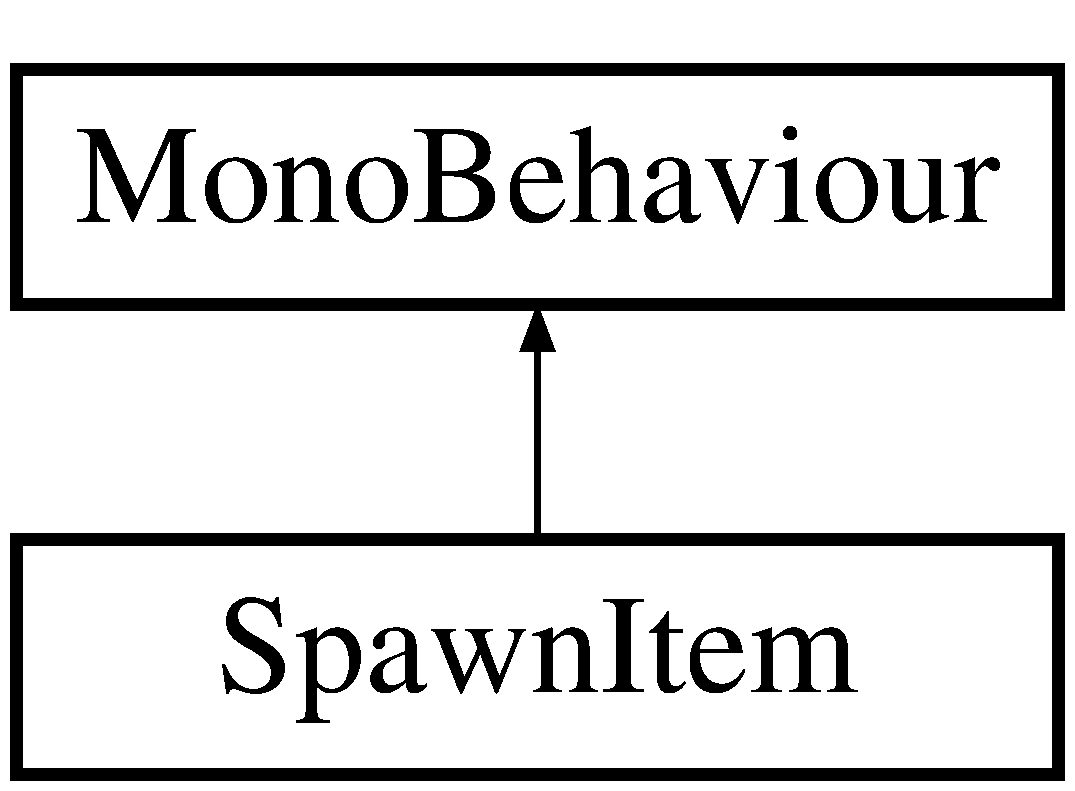
\includegraphics[height=2.000000cm]{class_spawn_item}
\end{center}
\end{figure}
\subsection*{Private Member Functions}
\begin{DoxyCompactItemize}
\item 
void \hyperlink{class_spawn_item_abce0af54142e123b9c4aae4fd6f4656c}{Start} ()
\item 
void \hyperlink{class_spawn_item_a0bcf186dd80f62583686eb240f2107ca}{Test} (string thign)
\item 
void \hyperlink{class_spawn_item_a51a14837f0e601a8487541d8ec502db9}{Update} ()
\item 
float \hyperlink{class_spawn_item_ac77536d30b5e96d90b03ea4b4ee5c2a8}{Rand} (float min, float max)
\item 
\hyperlink{namespace_bee_game_1_1_enums_aa2ead984825678d83c42d48f6382619c}{Bee\+Species} \hyperlink{class_spawn_item_af8aa1bfe3ed53c05d673dd46b26bc97e}{Get\+Random\+Item} ()
\end{DoxyCompactItemize}
\subsection*{Private Attributes}
\begin{DoxyCompactItemize}
\item 
\hyperlink{namespace_bee_game_1_1_enums_aa2ead984825678d83c42d48f6382619c}{Bee\+Species} \mbox{[}$\,$\mbox{]} \hyperlink{class_spawn_item_a0af51e744d43adcc6a295222b5d70a6e}{species} = new \hyperlink{namespace_bee_game_1_1_enums_aa2ead984825678d83c42d48f6382619c}{Bee\+Species}\mbox{[}4\mbox{]} \{ Bee\+Species.\+A\+G\+R\+A\+R\+I\+AN, Bee\+Species.\+A\+U\+S\+T\+ER, Bee\+Species.\+A\+V\+E\+N\+G\+I\+NG, Bee\+Species.\+B\+O\+G\+GY \}
\item 
float \mbox{[}$\,$\mbox{]} \hyperlink{class_spawn_item_a52966f3825c8c50f79c0a9a1ba300b52}{weights} = new float\mbox{[}4\mbox{]} \{ 0.\+5f, 0.\+1f, 0.\+2f, 0.\+2f \}
\end{DoxyCompactItemize}


\subsection{Detailed Description}


Definition at line 9 of file Spawn\+Item.\+cs.



\subsection{Member Function Documentation}
\mbox{\Hypertarget{class_spawn_item_af8aa1bfe3ed53c05d673dd46b26bc97e}\label{class_spawn_item_af8aa1bfe3ed53c05d673dd46b26bc97e}} 
\index{Spawn\+Item@{Spawn\+Item}!Get\+Random\+Item@{Get\+Random\+Item}}
\index{Get\+Random\+Item@{Get\+Random\+Item}!Spawn\+Item@{Spawn\+Item}}
\subsubsection{\texorpdfstring{Get\+Random\+Item()}{GetRandomItem()}}
{\footnotesize\ttfamily \hyperlink{namespace_bee_game_1_1_enums_aa2ead984825678d83c42d48f6382619c}{Bee\+Species} Spawn\+Item.\+Get\+Random\+Item (\begin{DoxyParamCaption}{ }\end{DoxyParamCaption})\hspace{0.3cm}{\ttfamily [private]}}



Definition at line 43 of file Spawn\+Item.\+cs.


\begin{DoxyCode}
44     \{
45         var totalWeight = 0f;
46 
47         \textcolor{keywordflow}{for} (\textcolor{keywordtype}{int} i = 0; i < \hyperlink{class_spawn_item_a52966f3825c8c50f79c0a9a1ba300b52}{weights}.Length; i++)
48         \{
49             totalWeight += \hyperlink{class_spawn_item_a52966f3825c8c50f79c0a9a1ba300b52}{weights}[i];
50         \}
51 
52         var randomNum = \hyperlink{class_spawn_item_ac77536d30b5e96d90b03ea4b4ee5c2a8}{Rand}(0, totalWeight);
53         Math.Round(randomNum, 2);
54         var weightSum = 0f;
55 
56         \textcolor{keywordflow}{for} (\textcolor{keywordtype}{int} i = 0; i < \hyperlink{class_spawn_item_a0af51e744d43adcc6a295222b5d70a6e}{species}.Length; i++)
57         \{
58             weightSum += \hyperlink{class_spawn_item_a52966f3825c8c50f79c0a9a1ba300b52}{weights}[i];
59 
60             \textcolor{keywordflow}{if} ((\textcolor{keywordtype}{float})randomNum <= weightSum)
61             \{
62                 \textcolor{keywordflow}{return} \hyperlink{class_spawn_item_a0af51e744d43adcc6a295222b5d70a6e}{species}[i];
63             \}
64         \}
65 
66         \textcolor{keywordflow}{return} 0;
67     \}
\end{DoxyCode}
\mbox{\Hypertarget{class_spawn_item_ac77536d30b5e96d90b03ea4b4ee5c2a8}\label{class_spawn_item_ac77536d30b5e96d90b03ea4b4ee5c2a8}} 
\index{Spawn\+Item@{Spawn\+Item}!Rand@{Rand}}
\index{Rand@{Rand}!Spawn\+Item@{Spawn\+Item}}
\subsubsection{\texorpdfstring{Rand()}{Rand()}}
{\footnotesize\ttfamily float Spawn\+Item.\+Rand (\begin{DoxyParamCaption}\item[{float}]{min,  }\item[{float}]{max }\end{DoxyParamCaption})\hspace{0.3cm}{\ttfamily [private]}}



Definition at line 35 of file Spawn\+Item.\+cs.


\begin{DoxyCode}
36     \{
37         \hyperlink{namespace_unity_engine}{UnityEngine}.Random rand = \textcolor{keyword}{new} \hyperlink{namespace_unity_engine}{UnityEngine}.Random();
38         \textcolor{keywordtype}{float} number = (max - min);
39 
40         \textcolor{keywordflow}{return} \hyperlink{namespace_unity_engine}{UnityEngine}.Random.Range(min, number);
41     \}
\end{DoxyCode}
\mbox{\Hypertarget{class_spawn_item_abce0af54142e123b9c4aae4fd6f4656c}\label{class_spawn_item_abce0af54142e123b9c4aae4fd6f4656c}} 
\index{Spawn\+Item@{Spawn\+Item}!Start@{Start}}
\index{Start@{Start}!Spawn\+Item@{Spawn\+Item}}
\subsubsection{\texorpdfstring{Start()}{Start()}}
{\footnotesize\ttfamily void Spawn\+Item.\+Start (\begin{DoxyParamCaption}{ }\end{DoxyParamCaption})\hspace{0.3cm}{\ttfamily [private]}}



Definition at line 14 of file Spawn\+Item.\+cs.


\begin{DoxyCode}
15     \{
16         \textcolor{comment}{//Item item = new Item("1");}
17         \textcolor{comment}{//item.ApplyDefaultBeeData(BeeSpecies.FOREST);}
18         \textcolor{comment}{//item.SetBeeType(BeeType.PRINCESS);}
19 
20         \textcolor{comment}{//GameObject temp = Instantiate(item.itemGameobject);}
21         \textcolor{comment}{//temp.GetComponent<ItemGameObjectInterface>().item = item;}
22         \textcolor{comment}{//QuestManager.beeMade += Test;}
23     \}
\end{DoxyCode}
\mbox{\Hypertarget{class_spawn_item_a0bcf186dd80f62583686eb240f2107ca}\label{class_spawn_item_a0bcf186dd80f62583686eb240f2107ca}} 
\index{Spawn\+Item@{Spawn\+Item}!Test@{Test}}
\index{Test@{Test}!Spawn\+Item@{Spawn\+Item}}
\subsubsection{\texorpdfstring{Test()}{Test()}}
{\footnotesize\ttfamily void Spawn\+Item.\+Test (\begin{DoxyParamCaption}\item[{string}]{thign }\end{DoxyParamCaption})\hspace{0.3cm}{\ttfamily [private]}}



Definition at line 25 of file Spawn\+Item.\+cs.


\begin{DoxyCode}
26     \{
27         print(thign);
28     \}
\end{DoxyCode}
\mbox{\Hypertarget{class_spawn_item_a51a14837f0e601a8487541d8ec502db9}\label{class_spawn_item_a51a14837f0e601a8487541d8ec502db9}} 
\index{Spawn\+Item@{Spawn\+Item}!Update@{Update}}
\index{Update@{Update}!Spawn\+Item@{Spawn\+Item}}
\subsubsection{\texorpdfstring{Update()}{Update()}}
{\footnotesize\ttfamily void Spawn\+Item.\+Update (\begin{DoxyParamCaption}{ }\end{DoxyParamCaption})\hspace{0.3cm}{\ttfamily [private]}}



Definition at line 30 of file Spawn\+Item.\+cs.


\begin{DoxyCode}
31     \{
32         \textcolor{comment}{//print(GetRandomItem());}
33     \}
\end{DoxyCode}


\subsection{Member Data Documentation}
\mbox{\Hypertarget{class_spawn_item_a0af51e744d43adcc6a295222b5d70a6e}\label{class_spawn_item_a0af51e744d43adcc6a295222b5d70a6e}} 
\index{Spawn\+Item@{Spawn\+Item}!species@{species}}
\index{species@{species}!Spawn\+Item@{Spawn\+Item}}
\subsubsection{\texorpdfstring{species}{species}}
{\footnotesize\ttfamily \hyperlink{namespace_bee_game_1_1_enums_aa2ead984825678d83c42d48f6382619c}{Bee\+Species} \mbox{[}$\,$\mbox{]} Spawn\+Item.\+species = new \hyperlink{namespace_bee_game_1_1_enums_aa2ead984825678d83c42d48f6382619c}{Bee\+Species}\mbox{[}4\mbox{]} \{ Bee\+Species.\+A\+G\+R\+A\+R\+I\+AN, Bee\+Species.\+A\+U\+S\+T\+ER, Bee\+Species.\+A\+V\+E\+N\+G\+I\+NG, Bee\+Species.\+B\+O\+G\+GY \}\hspace{0.3cm}{\ttfamily [private]}}



Definition at line 11 of file Spawn\+Item.\+cs.

\mbox{\Hypertarget{class_spawn_item_a52966f3825c8c50f79c0a9a1ba300b52}\label{class_spawn_item_a52966f3825c8c50f79c0a9a1ba300b52}} 
\index{Spawn\+Item@{Spawn\+Item}!weights@{weights}}
\index{weights@{weights}!Spawn\+Item@{Spawn\+Item}}
\subsubsection{\texorpdfstring{weights}{weights}}
{\footnotesize\ttfamily float \mbox{[}$\,$\mbox{]} Spawn\+Item.\+weights = new float\mbox{[}4\mbox{]} \{ 0.\+5f, 0.\+1f, 0.\+2f, 0.\+2f \}\hspace{0.3cm}{\ttfamily [private]}}



Definition at line 12 of file Spawn\+Item.\+cs.



The documentation for this class was generated from the following file\+:\begin{DoxyCompactItemize}
\item 
C\+:/\+Users/\+Toothless/\+Documents/\+Git\+Hub/\+Bee\+Game/\+Code/\+Bee\+Game/\+Bee\+Game/test/\hyperlink{_spawn_item_8cs}{Spawn\+Item.\+cs}\end{DoxyCompactItemize}

\hypertarget{class_bee_game_1_1_core_1_1_sprite_dictionary}{}\section{Bee\+Game.\+Core.\+Sprite\+Dictionary Class Reference}
\label{class_bee_game_1_1_core_1_1_sprite_dictionary}\index{Bee\+Game.\+Core.\+Sprite\+Dictionary@{Bee\+Game.\+Core.\+Sprite\+Dictionary}}
\subsection*{Static Public Member Functions}
\begin{DoxyCompactItemize}
\item 
static string \hyperlink{class_bee_game_1_1_core_1_1_sprite_dictionary_ae4d45a1450cc2a99493ca8aee6ebaab6}{Key} ()
\item 
static void \hyperlink{class_bee_game_1_1_core_1_1_sprite_dictionary_a55f237ff9c91a35b88adab2a4be844ed}{Add\+To\+Sprite\+Dictionary} (string sprite\+Name, Sprite sprite\+To\+Add)
\begin{DoxyCompactList}\small\item\em Adds a sprite to the dictionary \end{DoxyCompactList}\item 
static Sprite \hyperlink{class_bee_game_1_1_core_1_1_sprite_dictionary_a17fca1828cb89197a540e2e7ab0c43cd}{Get\+Sprite\+Item\+From\+Dictionary} (string sprite\+Name)
\begin{DoxyCompactList}\small\item\em Returns a Sprite fromthe given sprite name \end{DoxyCompactList}\end{DoxyCompactItemize}
\subsection*{Static Public Attributes}
\begin{DoxyCompactItemize}
\item 
static Dictionary$<$ string, Sprite $>$ \hyperlink{class_bee_game_1_1_core_1_1_sprite_dictionary_a40c5e9e2f9f25548971faadbbbde4529}{sprites} = new Dictionary$<$string, Sprite$>$()
\begin{DoxyCompactList}\small\item\em Stores all sprites that can be loaded by the game \end{DoxyCompactList}\end{DoxyCompactItemize}


\subsection{Detailed Description}


Definition at line 8 of file Sprite\+Dictionary.\+cs.



\subsection{Member Function Documentation}
\mbox{\Hypertarget{class_bee_game_1_1_core_1_1_sprite_dictionary_a55f237ff9c91a35b88adab2a4be844ed}\label{class_bee_game_1_1_core_1_1_sprite_dictionary_a55f237ff9c91a35b88adab2a4be844ed}} 
\index{Bee\+Game\+::\+Core\+::\+Sprite\+Dictionary@{Bee\+Game\+::\+Core\+::\+Sprite\+Dictionary}!Add\+To\+Sprite\+Dictionary@{Add\+To\+Sprite\+Dictionary}}
\index{Add\+To\+Sprite\+Dictionary@{Add\+To\+Sprite\+Dictionary}!Bee\+Game\+::\+Core\+::\+Sprite\+Dictionary@{Bee\+Game\+::\+Core\+::\+Sprite\+Dictionary}}
\subsubsection{\texorpdfstring{Add\+To\+Sprite\+Dictionary()}{AddToSpriteDictionary()}}
{\footnotesize\ttfamily static void Bee\+Game.\+Core.\+Sprite\+Dictionary.\+Add\+To\+Sprite\+Dictionary (\begin{DoxyParamCaption}\item[{string}]{sprite\+Name,  }\item[{Sprite}]{sprite\+To\+Add }\end{DoxyParamCaption})\hspace{0.3cm}{\ttfamily [static]}}



Adds a sprite to the dictionary 


\begin{DoxyParams}{Parameters}
{\em sprite\+Name} & Name of sprite\\
\hline
{\em sprite\+To\+Add} & Sprite\\
\hline
\end{DoxyParams}


Definition at line 31 of file Sprite\+Dictionary.\+cs.


\begin{DoxyCode}
32         \{
33             \textcolor{keywordflow}{if} (\hyperlink{class_bee_game_1_1_core_1_1_sprite_dictionary_a17fca1828cb89197a540e2e7ab0c43cd}{GetSpriteItemFromDictionary}(spriteName) == null)
34             \{
35                 \hyperlink{class_bee_game_1_1_core_1_1_sprite_dictionary_a40c5e9e2f9f25548971faadbbbde4529}{sprites}.Add(spriteName, spriteToAdd);
36             \}
37             \textcolor{keywordflow}{else}
38             \{
39                 \hyperlink{class_bee_game_1_1_core_1_1_sprite_dictionary_a40c5e9e2f9f25548971faadbbbde4529}{sprites}[spriteName] = spriteToAdd;
40             \}
41         \}
\end{DoxyCode}
\mbox{\Hypertarget{class_bee_game_1_1_core_1_1_sprite_dictionary_a17fca1828cb89197a540e2e7ab0c43cd}\label{class_bee_game_1_1_core_1_1_sprite_dictionary_a17fca1828cb89197a540e2e7ab0c43cd}} 
\index{Bee\+Game\+::\+Core\+::\+Sprite\+Dictionary@{Bee\+Game\+::\+Core\+::\+Sprite\+Dictionary}!Get\+Sprite\+Item\+From\+Dictionary@{Get\+Sprite\+Item\+From\+Dictionary}}
\index{Get\+Sprite\+Item\+From\+Dictionary@{Get\+Sprite\+Item\+From\+Dictionary}!Bee\+Game\+::\+Core\+::\+Sprite\+Dictionary@{Bee\+Game\+::\+Core\+::\+Sprite\+Dictionary}}
\subsubsection{\texorpdfstring{Get\+Sprite\+Item\+From\+Dictionary()}{GetSpriteItemFromDictionary()}}
{\footnotesize\ttfamily static Sprite Bee\+Game.\+Core.\+Sprite\+Dictionary.\+Get\+Sprite\+Item\+From\+Dictionary (\begin{DoxyParamCaption}\item[{string}]{sprite\+Name }\end{DoxyParamCaption})\hspace{0.3cm}{\ttfamily [static]}}



Returns a Sprite fromthe given sprite name 


\begin{DoxyParams}{Parameters}
{\em sprite\+Name} & Item sprite name\\
\hline
\end{DoxyParams}
\begin{DoxyReturn}{Returns}
Sprite
\end{DoxyReturn}


Definition at line 48 of file Sprite\+Dictionary.\+cs.


\begin{DoxyCode}
49         \{
50             \textcolor{keywordflow}{if} (spriteName != null)
51             \{
52                 \textcolor{keywordflow}{if} (\hyperlink{class_bee_game_1_1_core_1_1_sprite_dictionary_a40c5e9e2f9f25548971faadbbbde4529}{sprites}.ContainsKey(spriteName))
53                 \{
54                     \textcolor{keywordflow}{return} \hyperlink{class_bee_game_1_1_core_1_1_sprite_dictionary_a40c5e9e2f9f25548971faadbbbde4529}{sprites}[spriteName];
55                 \}
56             \}
57             
58             \textcolor{keywordflow}{return} null;
59         \}
\end{DoxyCode}
\mbox{\Hypertarget{class_bee_game_1_1_core_1_1_sprite_dictionary_ae4d45a1450cc2a99493ca8aee6ebaab6}\label{class_bee_game_1_1_core_1_1_sprite_dictionary_ae4d45a1450cc2a99493ca8aee6ebaab6}} 
\index{Bee\+Game\+::\+Core\+::\+Sprite\+Dictionary@{Bee\+Game\+::\+Core\+::\+Sprite\+Dictionary}!Key@{Key}}
\index{Key@{Key}!Bee\+Game\+::\+Core\+::\+Sprite\+Dictionary@{Bee\+Game\+::\+Core\+::\+Sprite\+Dictionary}}
\subsubsection{\texorpdfstring{Key()}{Key()}}
{\footnotesize\ttfamily static string Bee\+Game.\+Core.\+Sprite\+Dictionary.\+Key (\begin{DoxyParamCaption}{ }\end{DoxyParamCaption})\hspace{0.3cm}{\ttfamily [static]}}



Definition at line 15 of file Sprite\+Dictionary.\+cs.


\begin{DoxyCode}
16         \{
17             \textcolor{keywordtype}{string} returnKeys = \textcolor{stringliteral}{""};
18             \textcolor{keywordflow}{foreach}(\textcolor{keywordtype}{string} k \textcolor{keywordflow}{in} \hyperlink{class_bee_game_1_1_core_1_1_sprite_dictionary_a40c5e9e2f9f25548971faadbbbde4529}{sprites}.Keys)
19             \{
20                 returnKeys += k + \textcolor{stringliteral}{" "};
21             \}
22 
23             \textcolor{keywordflow}{return} returnKeys;
24         \}
\end{DoxyCode}


\subsection{Member Data Documentation}
\mbox{\Hypertarget{class_bee_game_1_1_core_1_1_sprite_dictionary_a40c5e9e2f9f25548971faadbbbde4529}\label{class_bee_game_1_1_core_1_1_sprite_dictionary_a40c5e9e2f9f25548971faadbbbde4529}} 
\index{Bee\+Game\+::\+Core\+::\+Sprite\+Dictionary@{Bee\+Game\+::\+Core\+::\+Sprite\+Dictionary}!sprites@{sprites}}
\index{sprites@{sprites}!Bee\+Game\+::\+Core\+::\+Sprite\+Dictionary@{Bee\+Game\+::\+Core\+::\+Sprite\+Dictionary}}
\subsubsection{\texorpdfstring{sprites}{sprites}}
{\footnotesize\ttfamily Dictionary$<$string, Sprite$>$ Bee\+Game.\+Core.\+Sprite\+Dictionary.\+sprites = new Dictionary$<$string, Sprite$>$()\hspace{0.3cm}{\ttfamily [static]}}



Stores all sprites that can be loaded by the game 



Definition at line 13 of file Sprite\+Dictionary.\+cs.



The documentation for this class was generated from the following file\+:\begin{DoxyCompactItemize}
\item 
C\+:/\+Users/\+Toothless/\+Documents/\+Git\+Hub/\+Bee\+Game/\+Code/\+Bee\+Game/\+Bee\+Game/\+Core/\hyperlink{_sprite_dictionary_8cs}{Sprite\+Dictionary.\+cs}\end{DoxyCompactItemize}

\hypertarget{struct_bee_game_1_1_t_h_vector3}{}\section{Bee\+Game.\+T\+H\+Vector3 Struct Reference}
\label{struct_bee_game_1_1_t_h_vector3}\index{Bee\+Game.\+T\+H\+Vector3@{Bee\+Game.\+T\+H\+Vector3}}
\subsection*{Public Member Functions}
\begin{DoxyCompactItemize}
\item 
\hyperlink{struct_bee_game_1_1_t_h_vector3_ad1b3467b019ea95fc114536aab566fb4}{T\+H\+Vector3} (Vector3 vector)
\item 
\hyperlink{struct_bee_game_1_1_t_h_vector3_aa2dd19cb61f71544d9126e647eb76b4b}{T\+H\+Vector3} (float \+\_\+x, float \+\_\+y, float \+\_\+z)
\item 
override int \hyperlink{struct_bee_game_1_1_t_h_vector3_a4a9942dbfb601a5c857676bc1dd25e43}{Get\+Hash\+Code} ()
\item 
override bool \hyperlink{struct_bee_game_1_1_t_h_vector3_af9efb591754dc8ec5994333babeed7d6}{Equals} (object b)
\end{DoxyCompactItemize}
\subsection*{Static Public Member Functions}
\begin{DoxyCompactItemize}
\item 
static bool \hyperlink{struct_bee_game_1_1_t_h_vector3_a34bd2c518136fe76411bba95f75cebdb}{operator==} (\hyperlink{struct_bee_game_1_1_t_h_vector3}{T\+H\+Vector3} a, \hyperlink{struct_bee_game_1_1_t_h_vector3}{T\+H\+Vector3} b)
\item 
static bool \hyperlink{struct_bee_game_1_1_t_h_vector3_a899f8d05be6344481d7411fee8b933a1}{operator!=} (\hyperlink{struct_bee_game_1_1_t_h_vector3}{T\+H\+Vector3} a, \hyperlink{struct_bee_game_1_1_t_h_vector3}{T\+H\+Vector3} b)
\item 
static \hyperlink{struct_bee_game_1_1_t_h_vector3}{T\+H\+Vector3} \hyperlink{struct_bee_game_1_1_t_h_vector3_a49eda0cb0ef9880dbcc9a60eaede8738}{operator+} (\hyperlink{struct_bee_game_1_1_t_h_vector3}{T\+H\+Vector3} a, \hyperlink{struct_bee_game_1_1_t_h_vector3}{T\+H\+Vector3} b)
\item 
static \hyperlink{struct_bee_game_1_1_t_h_vector3}{T\+H\+Vector3} \hyperlink{struct_bee_game_1_1_t_h_vector3_a036ff2d81d5be5ebbff5fe88555b6c79}{operator-\/} (\hyperlink{struct_bee_game_1_1_t_h_vector3}{T\+H\+Vector3} a, \hyperlink{struct_bee_game_1_1_t_h_vector3}{T\+H\+Vector3} b)
\item 
static \hyperlink{struct_bee_game_1_1_t_h_vector3}{T\+H\+Vector3} \hyperlink{struct_bee_game_1_1_t_h_vector3_a12e036f0743ac6ad26ac3b5c936c2b99}{operator$\ast$} (\hyperlink{struct_bee_game_1_1_t_h_vector3}{T\+H\+Vector3} a, \hyperlink{struct_bee_game_1_1_t_h_vector3}{T\+H\+Vector3} b)
\item 
static \hyperlink{struct_bee_game_1_1_t_h_vector3}{T\+H\+Vector3} \hyperlink{struct_bee_game_1_1_t_h_vector3_a62b6cab97890f7bb66c69c6f60bab04f}{operator$\ast$} (\hyperlink{struct_bee_game_1_1_t_h_vector3}{T\+H\+Vector3} a, float b)
\item 
static \hyperlink{struct_bee_game_1_1_t_h_vector3}{T\+H\+Vector3} \hyperlink{struct_bee_game_1_1_t_h_vector3_a465cd9dbaa1888ead6ea805852847e25}{operator/} (\hyperlink{struct_bee_game_1_1_t_h_vector3}{T\+H\+Vector3} a, \hyperlink{struct_bee_game_1_1_t_h_vector3}{T\+H\+Vector3} b)
\item 
static \hyperlink{struct_bee_game_1_1_t_h_vector3}{T\+H\+Vector3} \hyperlink{struct_bee_game_1_1_t_h_vector3_a20da6def0da94e1266e1b3ee56d2f299}{operator/} (\hyperlink{struct_bee_game_1_1_t_h_vector3}{T\+H\+Vector3} a, float b)
\end{DoxyCompactItemize}
\subsection*{Public Attributes}
\begin{DoxyCompactItemize}
\item 
float \hyperlink{struct_bee_game_1_1_t_h_vector3_a3a414a33eefb779cc52428463f428b6d}{x}
\item 
float \hyperlink{struct_bee_game_1_1_t_h_vector3_a58f88e615565042dbab4e4ba6ab1b3a6}{y}
\item 
float \hyperlink{struct_bee_game_1_1_t_h_vector3_a56c61f039a2cdabc8a371d2faa9838fa}{z}
\end{DoxyCompactItemize}


\subsection{Detailed Description}


Definition at line 8 of file T\+H\+Vector3.\+cs.



\subsection{Constructor \& Destructor Documentation}
\mbox{\Hypertarget{struct_bee_game_1_1_t_h_vector3_ad1b3467b019ea95fc114536aab566fb4}\label{struct_bee_game_1_1_t_h_vector3_ad1b3467b019ea95fc114536aab566fb4}} 
\index{Bee\+Game\+::\+T\+H\+Vector3@{Bee\+Game\+::\+T\+H\+Vector3}!T\+H\+Vector3@{T\+H\+Vector3}}
\index{T\+H\+Vector3@{T\+H\+Vector3}!Bee\+Game\+::\+T\+H\+Vector3@{Bee\+Game\+::\+T\+H\+Vector3}}
\subsubsection{\texorpdfstring{T\+H\+Vector3()}{THVector3()}\hspace{0.1cm}{\footnotesize\ttfamily [1/2]}}
{\footnotesize\ttfamily Bee\+Game.\+T\+H\+Vector3.\+T\+H\+Vector3 (\begin{DoxyParamCaption}\item[{Vector3}]{vector }\end{DoxyParamCaption})}



Definition at line 14 of file T\+H\+Vector3.\+cs.


\begin{DoxyCode}
15         \{
16             \hyperlink{struct_bee_game_1_1_t_h_vector3_a3a414a33eefb779cc52428463f428b6d}{x} = vector.x;
17             \hyperlink{struct_bee_game_1_1_t_h_vector3_a58f88e615565042dbab4e4ba6ab1b3a6}{y} = vector.y;
18             \hyperlink{struct_bee_game_1_1_t_h_vector3_a56c61f039a2cdabc8a371d2faa9838fa}{z} = vector.z;
19         \}
\end{DoxyCode}
\mbox{\Hypertarget{struct_bee_game_1_1_t_h_vector3_aa2dd19cb61f71544d9126e647eb76b4b}\label{struct_bee_game_1_1_t_h_vector3_aa2dd19cb61f71544d9126e647eb76b4b}} 
\index{Bee\+Game\+::\+T\+H\+Vector3@{Bee\+Game\+::\+T\+H\+Vector3}!T\+H\+Vector3@{T\+H\+Vector3}}
\index{T\+H\+Vector3@{T\+H\+Vector3}!Bee\+Game\+::\+T\+H\+Vector3@{Bee\+Game\+::\+T\+H\+Vector3}}
\subsubsection{\texorpdfstring{T\+H\+Vector3()}{THVector3()}\hspace{0.1cm}{\footnotesize\ttfamily [2/2]}}
{\footnotesize\ttfamily Bee\+Game.\+T\+H\+Vector3.\+T\+H\+Vector3 (\begin{DoxyParamCaption}\item[{float}]{\+\_\+x,  }\item[{float}]{\+\_\+y,  }\item[{float}]{\+\_\+z }\end{DoxyParamCaption})}



Definition at line 20 of file T\+H\+Vector3.\+cs.


\begin{DoxyCode}
21         \{
22             \hyperlink{struct_bee_game_1_1_t_h_vector3_a3a414a33eefb779cc52428463f428b6d}{x} = \_x;
23             \hyperlink{struct_bee_game_1_1_t_h_vector3_a58f88e615565042dbab4e4ba6ab1b3a6}{y} = \_y;
24             \hyperlink{struct_bee_game_1_1_t_h_vector3_a56c61f039a2cdabc8a371d2faa9838fa}{z} = \_z;
25         \}
\end{DoxyCode}


\subsection{Member Function Documentation}
\mbox{\Hypertarget{struct_bee_game_1_1_t_h_vector3_af9efb591754dc8ec5994333babeed7d6}\label{struct_bee_game_1_1_t_h_vector3_af9efb591754dc8ec5994333babeed7d6}} 
\index{Bee\+Game\+::\+T\+H\+Vector3@{Bee\+Game\+::\+T\+H\+Vector3}!Equals@{Equals}}
\index{Equals@{Equals}!Bee\+Game\+::\+T\+H\+Vector3@{Bee\+Game\+::\+T\+H\+Vector3}}
\subsubsection{\texorpdfstring{Equals()}{Equals()}}
{\footnotesize\ttfamily override bool Bee\+Game.\+T\+H\+Vector3.\+Equals (\begin{DoxyParamCaption}\item[{object}]{b }\end{DoxyParamCaption})}



Definition at line 32 of file T\+H\+Vector3.\+cs.


\begin{DoxyCode}
33         \{
34             \textcolor{keywordflow}{if} (b == null) \textcolor{keywordflow}{return} \textcolor{keyword}{false};
35             \textcolor{keywordflow}{if} (b.GetType() != GetType()) \textcolor{keywordflow}{return} \textcolor{keyword}{false};
36             \textcolor{keywordflow}{return} (\textcolor{keyword}{this} == (\hyperlink{struct_bee_game_1_1_t_h_vector3_ad1b3467b019ea95fc114536aab566fb4}{THVector3})b);
37         \}
\end{DoxyCode}
\mbox{\Hypertarget{struct_bee_game_1_1_t_h_vector3_a4a9942dbfb601a5c857676bc1dd25e43}\label{struct_bee_game_1_1_t_h_vector3_a4a9942dbfb601a5c857676bc1dd25e43}} 
\index{Bee\+Game\+::\+T\+H\+Vector3@{Bee\+Game\+::\+T\+H\+Vector3}!Get\+Hash\+Code@{Get\+Hash\+Code}}
\index{Get\+Hash\+Code@{Get\+Hash\+Code}!Bee\+Game\+::\+T\+H\+Vector3@{Bee\+Game\+::\+T\+H\+Vector3}}
\subsubsection{\texorpdfstring{Get\+Hash\+Code()}{GetHashCode()}}
{\footnotesize\ttfamily override int Bee\+Game.\+T\+H\+Vector3.\+Get\+Hash\+Code (\begin{DoxyParamCaption}{ }\end{DoxyParamCaption})}



Definition at line 28 of file T\+H\+Vector3.\+cs.


\begin{DoxyCode}
29         \{
30             \textcolor{keywordflow}{return} base.GetHashCode();
31         \}
\end{DoxyCode}
\mbox{\Hypertarget{struct_bee_game_1_1_t_h_vector3_a899f8d05be6344481d7411fee8b933a1}\label{struct_bee_game_1_1_t_h_vector3_a899f8d05be6344481d7411fee8b933a1}} 
\index{Bee\+Game\+::\+T\+H\+Vector3@{Bee\+Game\+::\+T\+H\+Vector3}!operator"!=@{operator"!=}}
\index{operator"!=@{operator"!=}!Bee\+Game\+::\+T\+H\+Vector3@{Bee\+Game\+::\+T\+H\+Vector3}}
\subsubsection{\texorpdfstring{operator"!=()}{operator!=()}}
{\footnotesize\ttfamily static bool Bee\+Game.\+T\+H\+Vector3.\+operator!= (\begin{DoxyParamCaption}\item[{\hyperlink{struct_bee_game_1_1_t_h_vector3}{T\+H\+Vector3}}]{a,  }\item[{\hyperlink{struct_bee_game_1_1_t_h_vector3}{T\+H\+Vector3}}]{b }\end{DoxyParamCaption})\hspace{0.3cm}{\ttfamily [static]}}



Definition at line 53 of file T\+H\+Vector3.\+cs.


\begin{DoxyCode}
54         \{
55             \textcolor{keywordflow}{return} !(a == b);
56         \}
\end{DoxyCode}
\mbox{\Hypertarget{struct_bee_game_1_1_t_h_vector3_a12e036f0743ac6ad26ac3b5c936c2b99}\label{struct_bee_game_1_1_t_h_vector3_a12e036f0743ac6ad26ac3b5c936c2b99}} 
\index{Bee\+Game\+::\+T\+H\+Vector3@{Bee\+Game\+::\+T\+H\+Vector3}!operator$\ast$@{operator$\ast$}}
\index{operator$\ast$@{operator$\ast$}!Bee\+Game\+::\+T\+H\+Vector3@{Bee\+Game\+::\+T\+H\+Vector3}}
\subsubsection{\texorpdfstring{operator$\ast$()}{operator*()}\hspace{0.1cm}{\footnotesize\ttfamily [1/2]}}
{\footnotesize\ttfamily static \hyperlink{struct_bee_game_1_1_t_h_vector3}{T\+H\+Vector3} Bee\+Game.\+T\+H\+Vector3.\+operator$\ast$ (\begin{DoxyParamCaption}\item[{\hyperlink{struct_bee_game_1_1_t_h_vector3}{T\+H\+Vector3}}]{a,  }\item[{\hyperlink{struct_bee_game_1_1_t_h_vector3}{T\+H\+Vector3}}]{b }\end{DoxyParamCaption})\hspace{0.3cm}{\ttfamily [static]}}



Definition at line 65 of file T\+H\+Vector3.\+cs.


\begin{DoxyCode}
66         \{
67             \textcolor{keywordflow}{return} \textcolor{keyword}{new} \hyperlink{struct_bee_game_1_1_t_h_vector3_ad1b3467b019ea95fc114536aab566fb4}{THVector3}(a.x * b.x, a.y * b.y, a.z * b.z);
68         \}
\end{DoxyCode}
\mbox{\Hypertarget{struct_bee_game_1_1_t_h_vector3_a62b6cab97890f7bb66c69c6f60bab04f}\label{struct_bee_game_1_1_t_h_vector3_a62b6cab97890f7bb66c69c6f60bab04f}} 
\index{Bee\+Game\+::\+T\+H\+Vector3@{Bee\+Game\+::\+T\+H\+Vector3}!operator$\ast$@{operator$\ast$}}
\index{operator$\ast$@{operator$\ast$}!Bee\+Game\+::\+T\+H\+Vector3@{Bee\+Game\+::\+T\+H\+Vector3}}
\subsubsection{\texorpdfstring{operator$\ast$()}{operator*()}\hspace{0.1cm}{\footnotesize\ttfamily [2/2]}}
{\footnotesize\ttfamily static \hyperlink{struct_bee_game_1_1_t_h_vector3}{T\+H\+Vector3} Bee\+Game.\+T\+H\+Vector3.\+operator$\ast$ (\begin{DoxyParamCaption}\item[{\hyperlink{struct_bee_game_1_1_t_h_vector3}{T\+H\+Vector3}}]{a,  }\item[{float}]{b }\end{DoxyParamCaption})\hspace{0.3cm}{\ttfamily [static]}}



Definition at line 69 of file T\+H\+Vector3.\+cs.


\begin{DoxyCode}
70         \{
71             \textcolor{keywordflow}{return} \textcolor{keyword}{new} \hyperlink{struct_bee_game_1_1_t_h_vector3_ad1b3467b019ea95fc114536aab566fb4}{THVector3}(a.x * b, a.y * b, a.z * b);
72         \}
\end{DoxyCode}
\mbox{\Hypertarget{struct_bee_game_1_1_t_h_vector3_a49eda0cb0ef9880dbcc9a60eaede8738}\label{struct_bee_game_1_1_t_h_vector3_a49eda0cb0ef9880dbcc9a60eaede8738}} 
\index{Bee\+Game\+::\+T\+H\+Vector3@{Bee\+Game\+::\+T\+H\+Vector3}!operator+@{operator+}}
\index{operator+@{operator+}!Bee\+Game\+::\+T\+H\+Vector3@{Bee\+Game\+::\+T\+H\+Vector3}}
\subsubsection{\texorpdfstring{operator+()}{operator+()}}
{\footnotesize\ttfamily static \hyperlink{struct_bee_game_1_1_t_h_vector3}{T\+H\+Vector3} Bee\+Game.\+T\+H\+Vector3.\+operator+ (\begin{DoxyParamCaption}\item[{\hyperlink{struct_bee_game_1_1_t_h_vector3}{T\+H\+Vector3}}]{a,  }\item[{\hyperlink{struct_bee_game_1_1_t_h_vector3}{T\+H\+Vector3}}]{b }\end{DoxyParamCaption})\hspace{0.3cm}{\ttfamily [static]}}



Definition at line 57 of file T\+H\+Vector3.\+cs.


\begin{DoxyCode}
58         \{
59             \textcolor{keywordflow}{return} \textcolor{keyword}{new} \hyperlink{struct_bee_game_1_1_t_h_vector3_ad1b3467b019ea95fc114536aab566fb4}{THVector3}(a.x + b.x, a.y + b.y, a.z + b.z);
60         \}
\end{DoxyCode}
\mbox{\Hypertarget{struct_bee_game_1_1_t_h_vector3_a036ff2d81d5be5ebbff5fe88555b6c79}\label{struct_bee_game_1_1_t_h_vector3_a036ff2d81d5be5ebbff5fe88555b6c79}} 
\index{Bee\+Game\+::\+T\+H\+Vector3@{Bee\+Game\+::\+T\+H\+Vector3}!operator-\/@{operator-\/}}
\index{operator-\/@{operator-\/}!Bee\+Game\+::\+T\+H\+Vector3@{Bee\+Game\+::\+T\+H\+Vector3}}
\subsubsection{\texorpdfstring{operator-\/()}{operator-()}}
{\footnotesize\ttfamily static \hyperlink{struct_bee_game_1_1_t_h_vector3}{T\+H\+Vector3} Bee\+Game.\+T\+H\+Vector3.\+operator-\/ (\begin{DoxyParamCaption}\item[{\hyperlink{struct_bee_game_1_1_t_h_vector3}{T\+H\+Vector3}}]{a,  }\item[{\hyperlink{struct_bee_game_1_1_t_h_vector3}{T\+H\+Vector3}}]{b }\end{DoxyParamCaption})\hspace{0.3cm}{\ttfamily [static]}}



Definition at line 61 of file T\+H\+Vector3.\+cs.


\begin{DoxyCode}
62         \{
63             \textcolor{keywordflow}{return} \textcolor{keyword}{new} \hyperlink{struct_bee_game_1_1_t_h_vector3_ad1b3467b019ea95fc114536aab566fb4}{THVector3}(a.x - b.x, a.y - b.y, a.z - b.z);
64         \}
\end{DoxyCode}
\mbox{\Hypertarget{struct_bee_game_1_1_t_h_vector3_a465cd9dbaa1888ead6ea805852847e25}\label{struct_bee_game_1_1_t_h_vector3_a465cd9dbaa1888ead6ea805852847e25}} 
\index{Bee\+Game\+::\+T\+H\+Vector3@{Bee\+Game\+::\+T\+H\+Vector3}!operator/@{operator/}}
\index{operator/@{operator/}!Bee\+Game\+::\+T\+H\+Vector3@{Bee\+Game\+::\+T\+H\+Vector3}}
\subsubsection{\texorpdfstring{operator/()}{operator/()}\hspace{0.1cm}{\footnotesize\ttfamily [1/2]}}
{\footnotesize\ttfamily static \hyperlink{struct_bee_game_1_1_t_h_vector3}{T\+H\+Vector3} Bee\+Game.\+T\+H\+Vector3.\+operator/ (\begin{DoxyParamCaption}\item[{\hyperlink{struct_bee_game_1_1_t_h_vector3}{T\+H\+Vector3}}]{a,  }\item[{\hyperlink{struct_bee_game_1_1_t_h_vector3}{T\+H\+Vector3}}]{b }\end{DoxyParamCaption})\hspace{0.3cm}{\ttfamily [static]}}



Definition at line 73 of file T\+H\+Vector3.\+cs.


\begin{DoxyCode}
74         \{
75             \textcolor{keywordflow}{return} \textcolor{keyword}{new} \hyperlink{struct_bee_game_1_1_t_h_vector3_ad1b3467b019ea95fc114536aab566fb4}{THVector3}(a.x / b.x, a.y / b.y, a.z / b.z);
76         \}
\end{DoxyCode}
\mbox{\Hypertarget{struct_bee_game_1_1_t_h_vector3_a20da6def0da94e1266e1b3ee56d2f299}\label{struct_bee_game_1_1_t_h_vector3_a20da6def0da94e1266e1b3ee56d2f299}} 
\index{Bee\+Game\+::\+T\+H\+Vector3@{Bee\+Game\+::\+T\+H\+Vector3}!operator/@{operator/}}
\index{operator/@{operator/}!Bee\+Game\+::\+T\+H\+Vector3@{Bee\+Game\+::\+T\+H\+Vector3}}
\subsubsection{\texorpdfstring{operator/()}{operator/()}\hspace{0.1cm}{\footnotesize\ttfamily [2/2]}}
{\footnotesize\ttfamily static \hyperlink{struct_bee_game_1_1_t_h_vector3}{T\+H\+Vector3} Bee\+Game.\+T\+H\+Vector3.\+operator/ (\begin{DoxyParamCaption}\item[{\hyperlink{struct_bee_game_1_1_t_h_vector3}{T\+H\+Vector3}}]{a,  }\item[{float}]{b }\end{DoxyParamCaption})\hspace{0.3cm}{\ttfamily [static]}}



Definition at line 77 of file T\+H\+Vector3.\+cs.


\begin{DoxyCode}
78         \{
79             \textcolor{keywordflow}{return} \textcolor{keyword}{new} \hyperlink{struct_bee_game_1_1_t_h_vector3_ad1b3467b019ea95fc114536aab566fb4}{THVector3}(a.x / b, a.y / b, a.z / b);
80         \}
\end{DoxyCode}
\mbox{\Hypertarget{struct_bee_game_1_1_t_h_vector3_a34bd2c518136fe76411bba95f75cebdb}\label{struct_bee_game_1_1_t_h_vector3_a34bd2c518136fe76411bba95f75cebdb}} 
\index{Bee\+Game\+::\+T\+H\+Vector3@{Bee\+Game\+::\+T\+H\+Vector3}!operator==@{operator==}}
\index{operator==@{operator==}!Bee\+Game\+::\+T\+H\+Vector3@{Bee\+Game\+::\+T\+H\+Vector3}}
\subsubsection{\texorpdfstring{operator==()}{operator==()}}
{\footnotesize\ttfamily static bool Bee\+Game.\+T\+H\+Vector3.\+operator== (\begin{DoxyParamCaption}\item[{\hyperlink{struct_bee_game_1_1_t_h_vector3}{T\+H\+Vector3}}]{a,  }\item[{\hyperlink{struct_bee_game_1_1_t_h_vector3}{T\+H\+Vector3}}]{b }\end{DoxyParamCaption})\hspace{0.3cm}{\ttfamily [static]}}



Definition at line 41 of file T\+H\+Vector3.\+cs.


\begin{DoxyCode}
42         \{
43 
44             \textcolor{keywordflow}{if}(a.x == b.x && a.y == b.y && a.z == b.z)
45             \{
46                 \textcolor{keywordflow}{return} \textcolor{keyword}{true};
47             \}
48             \textcolor{keywordflow}{else}
49             \{
50                 \textcolor{keywordflow}{return} \textcolor{keyword}{false};
51             \}
52         \}
\end{DoxyCode}


\subsection{Member Data Documentation}
\mbox{\Hypertarget{struct_bee_game_1_1_t_h_vector3_a3a414a33eefb779cc52428463f428b6d}\label{struct_bee_game_1_1_t_h_vector3_a3a414a33eefb779cc52428463f428b6d}} 
\index{Bee\+Game\+::\+T\+H\+Vector3@{Bee\+Game\+::\+T\+H\+Vector3}!x@{x}}
\index{x@{x}!Bee\+Game\+::\+T\+H\+Vector3@{Bee\+Game\+::\+T\+H\+Vector3}}
\subsubsection{\texorpdfstring{x}{x}}
{\footnotesize\ttfamily float Bee\+Game.\+T\+H\+Vector3.\+x}



Definition at line 10 of file T\+H\+Vector3.\+cs.

\mbox{\Hypertarget{struct_bee_game_1_1_t_h_vector3_a58f88e615565042dbab4e4ba6ab1b3a6}\label{struct_bee_game_1_1_t_h_vector3_a58f88e615565042dbab4e4ba6ab1b3a6}} 
\index{Bee\+Game\+::\+T\+H\+Vector3@{Bee\+Game\+::\+T\+H\+Vector3}!y@{y}}
\index{y@{y}!Bee\+Game\+::\+T\+H\+Vector3@{Bee\+Game\+::\+T\+H\+Vector3}}
\subsubsection{\texorpdfstring{y}{y}}
{\footnotesize\ttfamily float Bee\+Game.\+T\+H\+Vector3.\+y}



Definition at line 11 of file T\+H\+Vector3.\+cs.

\mbox{\Hypertarget{struct_bee_game_1_1_t_h_vector3_a56c61f039a2cdabc8a371d2faa9838fa}\label{struct_bee_game_1_1_t_h_vector3_a56c61f039a2cdabc8a371d2faa9838fa}} 
\index{Bee\+Game\+::\+T\+H\+Vector3@{Bee\+Game\+::\+T\+H\+Vector3}!z@{z}}
\index{z@{z}!Bee\+Game\+::\+T\+H\+Vector3@{Bee\+Game\+::\+T\+H\+Vector3}}
\subsubsection{\texorpdfstring{z}{z}}
{\footnotesize\ttfamily float Bee\+Game.\+T\+H\+Vector3.\+z}



Definition at line 12 of file T\+H\+Vector3.\+cs.



The documentation for this struct was generated from the following file\+:\begin{DoxyCompactItemize}
\item 
C\+:/\+Users/\+Toothless/\+Documents/\+Git\+Hub/\+Bee\+Game/\+Code/\+Bee\+Game/\+Bee\+Game/\+Serialization/\hyperlink{_t_h_vector3_8cs}{T\+H\+Vector3.\+cs}\end{DoxyCompactItemize}

\chapter{File Documentation}
\hypertarget{_apiary_8cs}{}\section{C\+:/\+Users/\+Toothless/\+Documents/\+Git\+Hub/\+Bee\+Game/\+Code/\+Bee\+Game/\+Bee\+Game/\+Bee/\+Apiary.cs File Reference}
\label{_apiary_8cs}\index{C\+:/\+Users/\+Toothless/\+Documents/\+Git\+Hub/\+Bee\+Game/\+Code/\+Bee\+Game/\+Bee\+Game/\+Bee/\+Apiary.\+cs@{C\+:/\+Users/\+Toothless/\+Documents/\+Git\+Hub/\+Bee\+Game/\+Code/\+Bee\+Game/\+Bee\+Game/\+Bee/\+Apiary.\+cs}}
\subsection*{Classes}
\begin{DoxyCompactItemize}
\item 
class \hyperlink{class_bee_game_1_1_bee_1_1_apiary}{Bee\+Game.\+Bee.\+Apiary}
\end{DoxyCompactItemize}
\subsection*{Namespaces}
\begin{DoxyCompactItemize}
\item 
namespace \hyperlink{namespace_bee_game_1_1_bee}{Bee\+Game.\+Bee}
\end{DoxyCompactItemize}

\hypertarget{_bee_data_8cs}{}\section{C\+:/\+Users/\+Toothless/\+Documents/\+Git\+Hub/\+Bee\+Game/\+Code/\+Bee\+Game/\+Bee\+Game/\+Bee/\+Bee\+Data.cs File Reference}
\label{_bee_data_8cs}\index{C\+:/\+Users/\+Toothless/\+Documents/\+Git\+Hub/\+Bee\+Game/\+Code/\+Bee\+Game/\+Bee\+Game/\+Bee/\+Bee\+Data.\+cs@{C\+:/\+Users/\+Toothless/\+Documents/\+Git\+Hub/\+Bee\+Game/\+Code/\+Bee\+Game/\+Bee\+Game/\+Bee/\+Bee\+Data.\+cs}}
\subsection*{Classes}
\begin{DoxyCompactItemize}
\item 
struct \hyperlink{struct_bee_game_1_1_bee_1_1_bee_data}{Bee\+Game.\+Bee.\+Bee\+Data}
\begin{DoxyCompactList}\small\item\em Data Storgae for the \hyperlink{namespace_bee_game_1_1_bee}{Bee}\textquotesingle{}s in the game \end{DoxyCompactList}\item 
struct \hyperlink{struct_bee_game_1_1_bee_1_1_combining_bee_data}{Bee\+Game.\+Bee.\+Combining\+Bee\+Data}
\end{DoxyCompactItemize}
\subsection*{Namespaces}
\begin{DoxyCompactItemize}
\item 
namespace \hyperlink{namespace_bee_game_1_1_bee}{Bee\+Game.\+Bee}
\end{DoxyCompactItemize}

\hypertarget{_block_8cs}{}\section{C\+:/\+Users/\+Toothless/\+Documents/\+Git\+Hub/\+Bee\+Game/\+Code/\+Bee\+Game/\+Bee\+Game/\+Blocks/\+Block.cs File Reference}
\label{_block_8cs}\index{C\+:/\+Users/\+Toothless/\+Documents/\+Git\+Hub/\+Bee\+Game/\+Code/\+Bee\+Game/\+Bee\+Game/\+Blocks/\+Block.\+cs@{C\+:/\+Users/\+Toothless/\+Documents/\+Git\+Hub/\+Bee\+Game/\+Code/\+Bee\+Game/\+Bee\+Game/\+Blocks/\+Block.\+cs}}
\subsection*{Classes}
\begin{DoxyCompactItemize}
\item 
class \hyperlink{class_bee_game_1_1_blocks_1_1_block}{Bee\+Game.\+Blocks.\+Block}
\end{DoxyCompactItemize}
\subsection*{Namespaces}
\begin{DoxyCompactItemize}
\item 
namespace \hyperlink{namespace_bee_game_1_1_blocks}{Bee\+Game.\+Blocks}
\end{DoxyCompactItemize}

\hypertarget{_block_game_object_interface_8cs}{}\section{C\+:/\+Users/\+Toothless/\+Documents/\+Git\+Hub/\+Bee\+Game/\+Code/\+Bee\+Game/\+Bee\+Game/\+Blocks/\+Block\+Game\+Object\+Interface.cs File Reference}
\label{_block_game_object_interface_8cs}\index{C\+:/\+Users/\+Toothless/\+Documents/\+Git\+Hub/\+Bee\+Game/\+Code/\+Bee\+Game/\+Bee\+Game/\+Blocks/\+Block\+Game\+Object\+Interface.\+cs@{C\+:/\+Users/\+Toothless/\+Documents/\+Git\+Hub/\+Bee\+Game/\+Code/\+Bee\+Game/\+Bee\+Game/\+Blocks/\+Block\+Game\+Object\+Interface.\+cs}}
\subsection*{Classes}
\begin{DoxyCompactItemize}
\item 
class \hyperlink{class_bee_game_1_1_blocks_1_1_block_game_object_interface}{Bee\+Game.\+Blocks.\+Block\+Game\+Object\+Interface}
\begin{DoxyCompactList}\small\item\em Interface between Game\+Object and \hyperlink{class_bee_game_1_1_blocks_1_1_block}{Block} data as Mono\+Behaviour dreived classes are Non-\/\+Serializable using c\# Binary\+Formatter \end{DoxyCompactList}\end{DoxyCompactItemize}
\subsection*{Namespaces}
\begin{DoxyCompactItemize}
\item 
namespace \hyperlink{namespace_bee_game_1_1_blocks}{Bee\+Game.\+Blocks}
\end{DoxyCompactItemize}

\hypertarget{_bee_dictionary_equality_comparer_8cs}{}\section{C\+:/\+Users/\+Toothless/\+Documents/\+Git\+Hub/\+Bee\+Game/\+Code/\+Bee\+Game/\+Bee\+Game/\+Core/\+Bee\+Dictionary\+Equality\+Comparer.cs File Reference}
\label{_bee_dictionary_equality_comparer_8cs}\index{C\+:/\+Users/\+Toothless/\+Documents/\+Git\+Hub/\+Bee\+Game/\+Code/\+Bee\+Game/\+Bee\+Game/\+Core/\+Bee\+Dictionary\+Equality\+Comparer.\+cs@{C\+:/\+Users/\+Toothless/\+Documents/\+Git\+Hub/\+Bee\+Game/\+Code/\+Bee\+Game/\+Bee\+Game/\+Core/\+Bee\+Dictionary\+Equality\+Comparer.\+cs}}
\subsection*{Classes}
\begin{DoxyCompactItemize}
\item 
class \hyperlink{class_bee_game_1_1_core_1_1_bee_dictionary_equality_comparer}{Bee\+Game.\+Core.\+Bee\+Dictionary\+Equality\+Comparer}
\end{DoxyCompactItemize}
\subsection*{Namespaces}
\begin{DoxyCompactItemize}
\item 
namespace \hyperlink{namespace_bee_game_1_1_core}{Bee\+Game.\+Core}
\end{DoxyCompactItemize}

\hypertarget{_bee_dictionarys_8cs}{}\section{C\+:/\+Users/\+Toothless/\+Documents/\+Git\+Hub/\+Bee\+Game/\+Code/\+Bee\+Game/\+Bee\+Game/\+Core/\+Bee\+Dictionarys.cs File Reference}
\label{_bee_dictionarys_8cs}\index{C\+:/\+Users/\+Toothless/\+Documents/\+Git\+Hub/\+Bee\+Game/\+Code/\+Bee\+Game/\+Bee\+Game/\+Core/\+Bee\+Dictionarys.\+cs@{C\+:/\+Users/\+Toothless/\+Documents/\+Git\+Hub/\+Bee\+Game/\+Code/\+Bee\+Game/\+Bee\+Game/\+Core/\+Bee\+Dictionarys.\+cs}}
\subsection*{Classes}
\begin{DoxyCompactItemize}
\item 
class \hyperlink{class_bee_game_1_1_core_1_1_bee_dictionarys}{Bee\+Game.\+Core.\+Bee\+Dictionarys}
\end{DoxyCompactItemize}
\subsection*{Namespaces}
\begin{DoxyCompactItemize}
\item 
namespace \hyperlink{namespace_bee_game_1_1_core}{Bee\+Game.\+Core}
\end{DoxyCompactItemize}

\hypertarget{_extenstion_methods_8cs}{}\section{C\+:/\+Users/\+Toothless/\+Documents/\+Git\+Hub/\+Bee\+Game/\+Code/\+Bee\+Game/\+Bee\+Game/\+Core/\+Extenstion\+Methods.cs File Reference}
\label{_extenstion_methods_8cs}\index{C\+:/\+Users/\+Toothless/\+Documents/\+Git\+Hub/\+Bee\+Game/\+Code/\+Bee\+Game/\+Bee\+Game/\+Core/\+Extenstion\+Methods.\+cs@{C\+:/\+Users/\+Toothless/\+Documents/\+Git\+Hub/\+Bee\+Game/\+Code/\+Bee\+Game/\+Bee\+Game/\+Core/\+Extenstion\+Methods.\+cs}}
\subsection*{Classes}
\begin{DoxyCompactItemize}
\item 
class \hyperlink{class_bee_game_1_1_core_1_1_extenstion_methods}{Bee\+Game.\+Core.\+Extenstion\+Methods}
\end{DoxyCompactItemize}
\subsection*{Namespaces}
\begin{DoxyCompactItemize}
\item 
namespace \hyperlink{namespace_bee_game_1_1_core}{Bee\+Game.\+Core}
\end{DoxyCompactItemize}

\hypertarget{_input_manager_8cs}{}\section{C\+:/\+Users/\+Toothless/\+Documents/\+Git\+Hub/\+Bee\+Game/\+Code/\+Bee\+Game/\+Bee\+Game/\+Core/\+Input\+Manager.cs File Reference}
\label{_input_manager_8cs}\index{C\+:/\+Users/\+Toothless/\+Documents/\+Git\+Hub/\+Bee\+Game/\+Code/\+Bee\+Game/\+Bee\+Game/\+Core/\+Input\+Manager.\+cs@{C\+:/\+Users/\+Toothless/\+Documents/\+Git\+Hub/\+Bee\+Game/\+Code/\+Bee\+Game/\+Bee\+Game/\+Core/\+Input\+Manager.\+cs}}
\subsection*{Classes}
\begin{DoxyCompactItemize}
\item 
class \hyperlink{class_bee_game_1_1_core_1_1_input_manager}{Bee\+Game.\+Core.\+Input\+Manager}
\begin{DoxyCompactList}\small\item\em My implementation of the unity input system. Acts as a buffer layer to the unity system so that the input keys can be changed at runtime \end{DoxyCompactList}\end{DoxyCompactItemize}
\subsection*{Namespaces}
\begin{DoxyCompactItemize}
\item 
namespace \hyperlink{namespace_bee_game_1_1_core}{Bee\+Game.\+Core}
\end{DoxyCompactItemize}

\hypertarget{_item_dictionary_8cs}{}\section{C\+:/\+Users/\+Toothless/\+Documents/\+Git\+Hub/\+Bee\+Game/\+Code/\+Bee\+Game/\+Bee\+Game/\+Core/\+Item\+Dictionary.cs File Reference}
\label{_item_dictionary_8cs}\index{C\+:/\+Users/\+Toothless/\+Documents/\+Git\+Hub/\+Bee\+Game/\+Code/\+Bee\+Game/\+Bee\+Game/\+Core/\+Item\+Dictionary.\+cs@{C\+:/\+Users/\+Toothless/\+Documents/\+Git\+Hub/\+Bee\+Game/\+Code/\+Bee\+Game/\+Bee\+Game/\+Core/\+Item\+Dictionary.\+cs}}
\subsection*{Classes}
\begin{DoxyCompactItemize}
\item 
class \hyperlink{class_bee_game_1_1_core_1_1_item_dictionary}{Bee\+Game.\+Core.\+Item\+Dictionary}
\end{DoxyCompactItemize}
\subsection*{Namespaces}
\begin{DoxyCompactItemize}
\item 
namespace \hyperlink{namespace_bee_game_1_1_core}{Bee\+Game.\+Core}
\end{DoxyCompactItemize}

\hypertarget{_load_prefabs_8cs}{}\section{C\+:/\+Users/\+Toothless/\+Documents/\+Git\+Hub/\+Bee\+Game/\+Code/\+Bee\+Game/\+Bee\+Game/\+Core/\+Load\+Prefabs.cs File Reference}
\label{_load_prefabs_8cs}\index{C\+:/\+Users/\+Toothless/\+Documents/\+Git\+Hub/\+Bee\+Game/\+Code/\+Bee\+Game/\+Bee\+Game/\+Core/\+Load\+Prefabs.\+cs@{C\+:/\+Users/\+Toothless/\+Documents/\+Git\+Hub/\+Bee\+Game/\+Code/\+Bee\+Game/\+Bee\+Game/\+Core/\+Load\+Prefabs.\+cs}}
\subsection*{Classes}
\begin{DoxyCompactItemize}
\item 
class \hyperlink{class_bee_game_1_1_core_1_1_load_prefabs}{Bee\+Game.\+Core.\+Load\+Prefabs}
\end{DoxyCompactItemize}
\subsection*{Namespaces}
\begin{DoxyCompactItemize}
\item 
namespace \hyperlink{namespace_bee_game_1_1_core}{Bee\+Game.\+Core}
\end{DoxyCompactItemize}

\hypertarget{_load_sprites_8cs}{}\section{C\+:/\+Users/\+Toothless/\+Documents/\+Git\+Hub/\+Bee\+Game/\+Code/\+Bee\+Game/\+Bee\+Game/\+Core/\+Load\+Sprites.cs File Reference}
\label{_load_sprites_8cs}\index{C\+:/\+Users/\+Toothless/\+Documents/\+Git\+Hub/\+Bee\+Game/\+Code/\+Bee\+Game/\+Bee\+Game/\+Core/\+Load\+Sprites.\+cs@{C\+:/\+Users/\+Toothless/\+Documents/\+Git\+Hub/\+Bee\+Game/\+Code/\+Bee\+Game/\+Bee\+Game/\+Core/\+Load\+Sprites.\+cs}}
\subsection*{Classes}
\begin{DoxyCompactItemize}
\item 
class \hyperlink{class_bee_game_1_1_core_1_1_load_sprites}{Bee\+Game.\+Core.\+Load\+Sprites}
\end{DoxyCompactItemize}
\subsection*{Namespaces}
\begin{DoxyCompactItemize}
\item 
namespace \hyperlink{namespace_bee_game_1_1_core}{Bee\+Game.\+Core}
\end{DoxyCompactItemize}

\hypertarget{_prefab_dictionary_8cs}{}\section{C\+:/\+Users/\+Toothless/\+Documents/\+Git\+Hub/\+Bee\+Game/\+Code/\+Bee\+Game/\+Bee\+Game/\+Core/\+Prefab\+Dictionary.cs File Reference}
\label{_prefab_dictionary_8cs}\index{C\+:/\+Users/\+Toothless/\+Documents/\+Git\+Hub/\+Bee\+Game/\+Code/\+Bee\+Game/\+Bee\+Game/\+Core/\+Prefab\+Dictionary.\+cs@{C\+:/\+Users/\+Toothless/\+Documents/\+Git\+Hub/\+Bee\+Game/\+Code/\+Bee\+Game/\+Bee\+Game/\+Core/\+Prefab\+Dictionary.\+cs}}
\subsection*{Classes}
\begin{DoxyCompactItemize}
\item 
class \hyperlink{class_bee_game_1_1_core_1_1_prefab_dictionary}{Bee\+Game.\+Core.\+Prefab\+Dictionary}
\end{DoxyCompactItemize}
\subsection*{Namespaces}
\begin{DoxyCompactItemize}
\item 
namespace \hyperlink{namespace_bee_game_1_1_core}{Bee\+Game.\+Core}
\end{DoxyCompactItemize}

\hypertarget{_sprite_dictionary_8cs}{}\section{C\+:/\+Users/\+Toothless/\+Documents/\+Git\+Hub/\+Bee\+Game/\+Code/\+Bee\+Game/\+Bee\+Game/\+Core/\+Sprite\+Dictionary.cs File Reference}
\label{_sprite_dictionary_8cs}\index{C\+:/\+Users/\+Toothless/\+Documents/\+Git\+Hub/\+Bee\+Game/\+Code/\+Bee\+Game/\+Bee\+Game/\+Core/\+Sprite\+Dictionary.\+cs@{C\+:/\+Users/\+Toothless/\+Documents/\+Git\+Hub/\+Bee\+Game/\+Code/\+Bee\+Game/\+Bee\+Game/\+Core/\+Sprite\+Dictionary.\+cs}}
\subsection*{Classes}
\begin{DoxyCompactItemize}
\item 
class \hyperlink{class_bee_game_1_1_core_1_1_sprite_dictionary}{Bee\+Game.\+Core.\+Sprite\+Dictionary}
\end{DoxyCompactItemize}
\subsection*{Namespaces}
\begin{DoxyCompactItemize}
\item 
namespace \hyperlink{namespace_bee_game_1_1_core}{Bee\+Game.\+Core}
\end{DoxyCompactItemize}

\hypertarget{_enums_8cs}{}\section{C\+:/\+Users/\+Toothless/\+Documents/\+Git\+Hub/\+Bee\+Game/\+Code/\+Bee\+Game/\+Bee\+Game/\+Enums/\+Enums.cs File Reference}
\label{_enums_8cs}\index{C\+:/\+Users/\+Toothless/\+Documents/\+Git\+Hub/\+Bee\+Game/\+Code/\+Bee\+Game/\+Bee\+Game/\+Enums/\+Enums.\+cs@{C\+:/\+Users/\+Toothless/\+Documents/\+Git\+Hub/\+Bee\+Game/\+Code/\+Bee\+Game/\+Bee\+Game/\+Enums/\+Enums.\+cs}}
\subsection*{Namespaces}
\begin{DoxyCompactItemize}
\item 
namespace \hyperlink{namespace_bee_game_1_1_enums}{Bee\+Game.\+Enums}
\end{DoxyCompactItemize}
\subsection*{Enumerations}
\begin{DoxyCompactItemize}
\item 
enum \hyperlink{namespace_bee_game_1_1_enums_aa1fa1a04627915b8e72d3bb1c5c3fa82}{Bee\+Game.\+Enums.\+Item\+Type} \{ \hyperlink{namespace_bee_game_1_1_enums_aa1fa1a04627915b8e72d3bb1c5c3fa82a2b911c015ed17a423c74ab9987330e60}{Bee\+Game.\+Enums.\+Item\+Type.\+I\+T\+EM}, 
\hyperlink{namespace_bee_game_1_1_enums_aa1fa1a04627915b8e72d3bb1c5c3fa82a24af484e92082ad450a63a69f924f10a}{Bee\+Game.\+Enums.\+Item\+Type.\+B\+EE}
 \}\begin{DoxyCompactList}\small\item\em The item types \end{DoxyCompactList}
\item 
enum \hyperlink{namespace_bee_game_1_1_enums_aa2ead984825678d83c42d48f6382619c}{Bee\+Game.\+Enums.\+Bee\+Species} \{ \newline
\hyperlink{namespace_bee_game_1_1_enums_aa2ead984825678d83c42d48f6382619ca1868c2177fdc84d496f7784a23729d3b}{Bee\+Game.\+Enums.\+Bee\+Species.\+F\+O\+R\+E\+ST}, 
\hyperlink{namespace_bee_game_1_1_enums_aa2ead984825678d83c42d48f6382619cac9012ad3d12ac6e61b88f2871ae8984e}{Bee\+Game.\+Enums.\+Bee\+Species.\+M\+E\+A\+D\+O\+WS}, 
\hyperlink{namespace_bee_game_1_1_enums_aa2ead984825678d83c42d48f6382619cab2ef5f527a20dd2b0b0c4642685e1d1d}{Bee\+Game.\+Enums.\+Bee\+Species.\+T\+R\+O\+P\+I\+C\+AL}, 
\hyperlink{namespace_bee_game_1_1_enums_aa2ead984825678d83c42d48f6382619cab20dce50bacb833125b1c5cace0e8768}{Bee\+Game.\+Enums.\+Bee\+Species.\+W\+I\+N\+T\+RY}, 
\newline
\hyperlink{namespace_bee_game_1_1_enums_aa2ead984825678d83c42d48f6382619ca68a19b5ff536b017119a2dd44403b5fc}{Bee\+Game.\+Enums.\+Bee\+Species.\+M\+O\+D\+E\+ST}, 
\hyperlink{namespace_bee_game_1_1_enums_aa2ead984825678d83c42d48f6382619cab3dd49c780bfda9918403c9a4ccd4424}{Bee\+Game.\+Enums.\+Bee\+Species.\+M\+A\+R\+S\+HY}, 
\hyperlink{namespace_bee_game_1_1_enums_aa2ead984825678d83c42d48f6382619ca0d800016e1f76067cbc36701dd6c7609}{Bee\+Game.\+Enums.\+Bee\+Species.\+E\+N\+D\+ER}, 
\hyperlink{namespace_bee_game_1_1_enums_aa2ead984825678d83c42d48f6382619cacb30e522c4cde1b069a596b8a501800e}{Bee\+Game.\+Enums.\+Bee\+Species.\+M\+O\+N\+A\+S\+T\+IC}, 
\newline
\hyperlink{namespace_bee_game_1_1_enums_aa2ead984825678d83c42d48f6382619cabcabb595cf1e60ef02c699c24d4da140}{Bee\+Game.\+Enums.\+Bee\+Species.\+S\+T\+E\+A\+D\+F\+A\+ST}, 
\hyperlink{namespace_bee_game_1_1_enums_aa2ead984825678d83c42d48f6382619ca20e5116ef9046c3394b1fe42b883f8f5}{Bee\+Game.\+Enums.\+Bee\+Species.\+V\+A\+L\+I\+A\+NT}, 
\hyperlink{namespace_bee_game_1_1_enums_aa2ead984825678d83c42d48f6382619cadda4b7de10e14445366494f0a76e1435}{Bee\+Game.\+Enums.\+Bee\+Species.\+C\+O\+M\+M\+ON}, 
\hyperlink{namespace_bee_game_1_1_enums_aa2ead984825678d83c42d48f6382619ca40a11e6e0c3522e993244d76778046a0}{Bee\+Game.\+Enums.\+Bee\+Species.\+C\+U\+L\+T\+I\+V\+A\+T\+ED}, 
\newline
\hyperlink{namespace_bee_game_1_1_enums_aa2ead984825678d83c42d48f6382619ca317ab8c8b4ccd4ef02eac49bd97ed349}{Bee\+Game.\+Enums.\+Bee\+Species.\+D\+I\+L\+I\+G\+E\+NT}, 
\hyperlink{namespace_bee_game_1_1_enums_aa2ead984825678d83c42d48f6382619caea7c33d3a0fb3a1bc645a6116f54343a}{Bee\+Game.\+Enums.\+Bee\+Species.\+R\+U\+R\+AL}, 
\hyperlink{namespace_bee_game_1_1_enums_aa2ead984825678d83c42d48f6382619ca8946cbc468a699a0864c54d585508e07}{Bee\+Game.\+Enums.\+Bee\+Species.\+F\+A\+R\+M\+E\+R\+LY}, 
\hyperlink{namespace_bee_game_1_1_enums_aa2ead984825678d83c42d48f6382619ca18ad9d2be1cf1126a969b49b6b72f695}{Bee\+Game.\+Enums.\+Bee\+Species.\+A\+G\+R\+A\+R\+I\+AN}, 
\newline
\hyperlink{namespace_bee_game_1_1_enums_aa2ead984825678d83c42d48f6382619caba1f00f80faf55547b1237f301990889}{Bee\+Game.\+Enums.\+Bee\+Species.\+U\+N\+W\+E\+A\+RY}, 
\hyperlink{namespace_bee_game_1_1_enums_aa2ead984825678d83c42d48f6382619ca30b42f7a56ffbbab85c16b99a03a0f6e}{Bee\+Game.\+Enums.\+Bee\+Species.\+I\+N\+D\+U\+S\+T\+R\+I\+O\+US}, 
\hyperlink{namespace_bee_game_1_1_enums_aa2ead984825678d83c42d48f6382619ca5b33560a8f6238eb29adf382b23125e1}{Bee\+Game.\+Enums.\+Bee\+Species.\+I\+CY}, 
\hyperlink{namespace_bee_game_1_1_enums_aa2ead984825678d83c42d48f6382619ca4c6fdeaa6aeefb953e06e4bed5d2a137}{Bee\+Game.\+Enums.\+Bee\+Species.\+G\+L\+A\+C\+I\+AL}, 
\newline
\hyperlink{namespace_bee_game_1_1_enums_aa2ead984825678d83c42d48f6382619ca37820eb448c77df544abe7cee9e64222}{Bee\+Game.\+Enums.\+Bee\+Species.\+N\+O\+B\+LE}, 
\hyperlink{namespace_bee_game_1_1_enums_aa2ead984825678d83c42d48f6382619cad859c618456069308219a65d1747c63d}{Bee\+Game.\+Enums.\+Bee\+Species.\+I\+M\+P\+E\+R\+I\+AL}, 
\hyperlink{namespace_bee_game_1_1_enums_aa2ead984825678d83c42d48f6382619cac71022bd01e7a6e4f499352af54998e1}{Bee\+Game.\+Enums.\+Bee\+Species.\+M\+A\+J\+E\+C\+T\+IC}, 
\hyperlink{namespace_bee_game_1_1_enums_aa2ead984825678d83c42d48f6382619ca0e60c21f69944ed4923bb490b0f7f35e}{Bee\+Game.\+Enums.\+Bee\+Species.\+M\+I\+RY}, 
\newline
\hyperlink{namespace_bee_game_1_1_enums_aa2ead984825678d83c42d48f6382619cad646cd214438b9a785b04e2476a7fdbb}{Bee\+Game.\+Enums.\+Bee\+Species.\+B\+O\+G\+GY}, 
\hyperlink{namespace_bee_game_1_1_enums_aa2ead984825678d83c42d48f6382619ca9de82115e7089abc0da5c0a27e21668b}{Bee\+Game.\+Enums.\+Bee\+Species.\+H\+E\+R\+I\+OC}, 
\hyperlink{namespace_bee_game_1_1_enums_aa2ead984825678d83c42d48f6382619ca3e59cf577c2e411fd7aa15bef0a9c555}{Bee\+Game.\+Enums.\+Bee\+Species.\+P\+H\+A\+N\+T\+A\+S\+M\+AL}, 
\hyperlink{namespace_bee_game_1_1_enums_aa2ead984825678d83c42d48f6382619ca0ea0e24bfa104b610cbb50871bc1c9e7}{Bee\+Game.\+Enums.\+Bee\+Species.\+S\+P\+E\+C\+T\+R\+AL}, 
\newline
\hyperlink{namespace_bee_game_1_1_enums_aa2ead984825678d83c42d48f6382619cacba328231cbcc107bc33d8c5f7736f31}{Bee\+Game.\+Enums.\+Bee\+Species.\+H\+E\+R\+M\+E\+T\+IC}, 
\hyperlink{namespace_bee_game_1_1_enums_aa2ead984825678d83c42d48f6382619cafa4c4bd73d5828c6ec126a18e4cd18d1}{Bee\+Game.\+Enums.\+Bee\+Species.\+S\+E\+C\+L\+U\+D\+ED}, 
\hyperlink{namespace_bee_game_1_1_enums_aa2ead984825678d83c42d48f6382619cae82d85a038b6d6a9b5f4d3d1191e1d1f}{Bee\+Game.\+Enums.\+Bee\+Species.\+S\+I\+N\+I\+S\+T\+ER}, 
\hyperlink{namespace_bee_game_1_1_enums_aa2ead984825678d83c42d48f6382619ca5bf2c448e80896272e14fafa7450a4ff}{Bee\+Game.\+Enums.\+Bee\+Species.\+F\+I\+E\+N\+D\+I\+SH}, 
\newline
\hyperlink{namespace_bee_game_1_1_enums_aa2ead984825678d83c42d48f6382619ca3ef4f11188954e64884037cae7c3e963}{Bee\+Game.\+Enums.\+Bee\+Species.\+D\+E\+M\+O\+N\+IC}, 
\hyperlink{namespace_bee_game_1_1_enums_aa2ead984825678d83c42d48f6382619ca3b14a2f070412ad34ba4e889dedd815f}{Bee\+Game.\+Enums.\+Bee\+Species.\+F\+R\+U\+G\+AL}, 
\hyperlink{namespace_bee_game_1_1_enums_aa2ead984825678d83c42d48f6382619ca6b371bbc924baa10f0ed9c3e08c3b0cb}{Bee\+Game.\+Enums.\+Bee\+Species.\+A\+U\+S\+T\+ER}, 
\hyperlink{namespace_bee_game_1_1_enums_aa2ead984825678d83c42d48f6382619ca8f57d6b73edd27a6c0286071e7856f02}{Bee\+Game.\+Enums.\+Bee\+Species.\+V\+I\+N\+D\+I\+C\+T\+I\+VE}, 
\newline
\hyperlink{namespace_bee_game_1_1_enums_aa2ead984825678d83c42d48f6382619ca5c8d7464a13655925a110c502d9cbb2b}{Bee\+Game.\+Enums.\+Bee\+Species.\+E\+X\+O\+T\+IC}, 
\hyperlink{namespace_bee_game_1_1_enums_aa2ead984825678d83c42d48f6382619ca5472e7bd3b55f54a1bfb70a0d5a0e0da}{Bee\+Game.\+Enums.\+Bee\+Species.\+E\+N\+D\+E\+M\+IC}, 
\hyperlink{namespace_bee_game_1_1_enums_aa2ead984825678d83c42d48f6382619ca62d512056e515b0c590ac3a91bc37cf2}{Bee\+Game.\+Enums.\+Bee\+Species.\+V\+E\+N\+G\+E\+F\+UL}, 
\hyperlink{namespace_bee_game_1_1_enums_aa2ead984825678d83c42d48f6382619ca0db4fc841920b49db2210bcf7cd1ea87}{Bee\+Game.\+Enums.\+Bee\+Species.\+A\+V\+E\+N\+G\+I\+NG}, 
\newline
\hyperlink{namespace_bee_game_1_1_enums_aa2ead984825678d83c42d48f6382619ca6fd6e4d8dc13fe33a3a9959ecec4d42d}{Bee\+Game.\+Enums.\+Bee\+Species.\+S\+E\+T\+A\+D\+F\+A\+ST}, 
\hyperlink{namespace_bee_game_1_1_enums_aa2ead984825678d83c42d48f6382619ca48a3dc51512f82e9674ae151dbe1d41c}{Bee\+Game.\+Enums.\+Bee\+Species.\+H\+E\+R\+O\+IC}
 \}\begin{DoxyCompactList}\small\item\em The different possible bee Species \end{DoxyCompactList}
\item 
enum \hyperlink{namespace_bee_game_1_1_enums_a9376a1582db99d20c756e24de728944f}{Bee\+Game.\+Enums.\+Bee\+Type} \{ \hyperlink{namespace_bee_game_1_1_enums_a9376a1582db99d20c756e24de728944fa02d144e18eda99bcb94f3a764756805e}{Bee\+Game.\+Enums.\+Bee\+Type.\+Q\+U\+E\+EN}, 
\hyperlink{namespace_bee_game_1_1_enums_a9376a1582db99d20c756e24de728944fa3ca9340682c7fce45dcf786fc8232e0c}{Bee\+Game.\+Enums.\+Bee\+Type.\+P\+R\+I\+N\+C\+E\+SS}, 
\hyperlink{namespace_bee_game_1_1_enums_a9376a1582db99d20c756e24de728944fad3c26749c501de5924ed7ad5f621de4e}{Bee\+Game.\+Enums.\+Bee\+Type.\+D\+R\+O\+NE}
 \}\begin{DoxyCompactList}\small\item\em The different bee types \end{DoxyCompactList}
\item 
enum \hyperlink{namespace_bee_game_1_1_enums_a9db0f9ac859fab168654d657f248b024}{Bee\+Game.\+Enums.\+Bee\+Temp\+Preferance} \{ \newline
\hyperlink{namespace_bee_game_1_1_enums_a9db0f9ac859fab168654d657f248b024a081912e034fd835fdda076251f2cd586}{Bee\+Game.\+Enums.\+Bee\+Temp\+Preferance.\+F\+R\+O\+Z\+EN}, 
\hyperlink{namespace_bee_game_1_1_enums_a9db0f9ac859fab168654d657f248b024a3f7ff4daa99912d1b0c8c64340edb9fb}{Bee\+Game.\+Enums.\+Bee\+Temp\+Preferance.\+C\+O\+LD}, 
\hyperlink{namespace_bee_game_1_1_enums_a9db0f9ac859fab168654d657f248b024ad5938597ebb26919bd3b131a5f076b35}{Bee\+Game.\+Enums.\+Bee\+Temp\+Preferance.\+T\+E\+M\+P\+E\+R\+A\+TE}, 
\hyperlink{namespace_bee_game_1_1_enums_a9db0f9ac859fab168654d657f248b024ac429fde8b1b986d42f84ba63dbfef6ac}{Bee\+Game.\+Enums.\+Bee\+Temp\+Preferance.\+H\+OT}, 
\newline
\hyperlink{namespace_bee_game_1_1_enums_a9db0f9ac859fab168654d657f248b024a5fa58915fea0b7f3e0f1e8ec558a9123}{Bee\+Game.\+Enums.\+Bee\+Temp\+Preferance.\+H\+E\+LL}
 \}\begin{DoxyCompactList}\small\item\em The different bee temp preferences \end{DoxyCompactList}
\item 
enum \hyperlink{namespace_bee_game_1_1_enums_ae3853807ded2f4d99a0d4a7fb4b2bc46}{Bee\+Game.\+Enums.\+Bee\+Life\+Span} \{ \newline
\hyperlink{namespace_bee_game_1_1_enums_ae3853807ded2f4d99a0d4a7fb4b2bc46a2acefbb6f248411a587d402bfa3f17d2}{Bee\+Game.\+Enums.\+Bee\+Life\+Span.\+H\+U\+M\+M\+I\+N\+G\+B\+I\+RD}, 
\hyperlink{namespace_bee_game_1_1_enums_ae3853807ded2f4d99a0d4a7fb4b2bc46aa63ddb11bc6cc95583b3f7632a45a16b}{Bee\+Game.\+Enums.\+Bee\+Life\+Span.\+S\+H\+O\+R\+T\+E\+ST}, 
\hyperlink{namespace_bee_game_1_1_enums_ae3853807ded2f4d99a0d4a7fb4b2bc46aa35c2b02966b1563e5bf7b81b8b0cf77}{Bee\+Game.\+Enums.\+Bee\+Life\+Span.\+S\+H\+O\+RT}, 
\hyperlink{namespace_bee_game_1_1_enums_ae3853807ded2f4d99a0d4a7fb4b2bc46a1e23852820b9154316c7c06e2b7ba051}{Bee\+Game.\+Enums.\+Bee\+Life\+Span.\+N\+O\+R\+M\+AL}, 
\newline
\hyperlink{namespace_bee_game_1_1_enums_ae3853807ded2f4d99a0d4a7fb4b2bc46ac1fabfea54ec6011e694f211f3ffebf3}{Bee\+Game.\+Enums.\+Bee\+Life\+Span.\+L\+O\+NG}, 
\hyperlink{namespace_bee_game_1_1_enums_ae3853807ded2f4d99a0d4a7fb4b2bc46a9a377a4877bbfa6ed4037fc64476d739}{Bee\+Game.\+Enums.\+Bee\+Life\+Span.\+L\+O\+N\+G\+E\+ST}, 
\hyperlink{namespace_bee_game_1_1_enums_ae3853807ded2f4d99a0d4a7fb4b2bc46a264c8ca594c19cceea527c2965380f68}{Bee\+Game.\+Enums.\+Bee\+Life\+Span.\+S\+E\+A\+T\+U\+R\+T\+LE}
 \}\begin{DoxyCompactList}\small\item\em The lifespan of the bee \end{DoxyCompactList}
\item 
enum \hyperlink{namespace_bee_game_1_1_enums_afee18200a21cc4b8e1d0cdb669930f14}{Bee\+Game.\+Enums.\+Bee\+Production\+Speed} \{ \hyperlink{namespace_bee_game_1_1_enums_afee18200a21cc4b8e1d0cdb669930f14a0e3066cbbd284dce8b76e7c4620d6d75}{Bee\+Game.\+Enums.\+Bee\+Production\+Speed.\+S\+L\+OW}, 
\hyperlink{namespace_bee_game_1_1_enums_afee18200a21cc4b8e1d0cdb669930f14a1e23852820b9154316c7c06e2b7ba051}{Bee\+Game.\+Enums.\+Bee\+Production\+Speed.\+N\+O\+R\+M\+AL}, 
\hyperlink{namespace_bee_game_1_1_enums_afee18200a21cc4b8e1d0cdb669930f14adca6e617f6fb54033deb311e7e7c93cc}{Bee\+Game.\+Enums.\+Bee\+Production\+Speed.\+F\+A\+ST}
 \}\begin{DoxyCompactList}\small\item\em How fast the bee produces items \end{DoxyCompactList}
\item 
enum \hyperlink{namespace_bee_game_1_1_enums_acf7ae32a86385a40fc0c7b55af95c6c3}{Bee\+Game.\+Enums.\+Bee\+Effect} \{ \hyperlink{namespace_bee_game_1_1_enums_acf7ae32a86385a40fc0c7b55af95c6c3ab50339a10e1de285ac99d4c3990b8693}{Bee\+Game.\+Enums.\+Bee\+Effect.\+N\+O\+NE}, 
\hyperlink{namespace_bee_game_1_1_enums_acf7ae32a86385a40fc0c7b55af95c6c3a70a4c0cd10fc77f4e760429b2633d739}{Bee\+Game.\+Enums.\+Bee\+Effect.\+P\+O\+S\+I\+ON}
 \}\begin{DoxyCompactList}\small\item\em Any effects of the bee \end{DoxyCompactList}
\item 
enum \hyperlink{namespace_bee_game_1_1_enums_a66566cbc9da8d1d1e402156b4bd3bf9d}{Bee\+Game.\+Enums.\+Bee\+Humidity\+Preferance} \{ \newline
\hyperlink{namespace_bee_game_1_1_enums_a66566cbc9da8d1d1e402156b4bd3bf9dacb2b7bbb0e2f3f76538306e5fa548770}{Bee\+Game.\+Enums.\+Bee\+Humidity\+Preferance.\+A\+R\+ID}, 
\hyperlink{namespace_bee_game_1_1_enums_a66566cbc9da8d1d1e402156b4bd3bf9da76cca64663bcf77e11df2d5a88fc7d4b}{Bee\+Game.\+Enums.\+Bee\+Humidity\+Preferance.\+D\+RY}, 
\hyperlink{namespace_bee_game_1_1_enums_a66566cbc9da8d1d1e402156b4bd3bf9dad5938597ebb26919bd3b131a5f076b35}{Bee\+Game.\+Enums.\+Bee\+Humidity\+Preferance.\+T\+E\+M\+P\+E\+R\+A\+TE}, 
\hyperlink{namespace_bee_game_1_1_enums_a66566cbc9da8d1d1e402156b4bd3bf9da8c810d76ac96d2a8ddfe7b859307ad1f}{Bee\+Game.\+Enums.\+Bee\+Humidity\+Preferance.\+M\+O\+I\+ST}, 
\newline
\hyperlink{namespace_bee_game_1_1_enums_a66566cbc9da8d1d1e402156b4bd3bf9dae21803baeeb8740c4616bc69a5e35b40}{Bee\+Game.\+Enums.\+Bee\+Humidity\+Preferance.\+H\+U\+M\+ID}
 \}\begin{DoxyCompactList}\small\item\em Humidity preferences of the bee \end{DoxyCompactList}
\end{DoxyCompactItemize}

\hypertarget{_chest_inventory_8cs}{}\section{C\+:/\+Users/\+Toothless/\+Documents/\+Git\+Hub/\+Bee\+Game/\+Code/\+Bee\+Game/\+Bee\+Game/\+Inventory/\+Chest\+Inventory.cs File Reference}
\label{_chest_inventory_8cs}\index{C\+:/\+Users/\+Toothless/\+Documents/\+Git\+Hub/\+Bee\+Game/\+Code/\+Bee\+Game/\+Bee\+Game/\+Inventory/\+Chest\+Inventory.\+cs@{C\+:/\+Users/\+Toothless/\+Documents/\+Git\+Hub/\+Bee\+Game/\+Code/\+Bee\+Game/\+Bee\+Game/\+Inventory/\+Chest\+Inventory.\+cs}}
\subsection*{Classes}
\begin{DoxyCompactItemize}
\item 
class \hyperlink{class_bee_game_1_1_inventory_1_1_chest_inventory}{Bee\+Game.\+Inventory.\+Chest\+Inventory}
\end{DoxyCompactItemize}
\subsection*{Namespaces}
\begin{DoxyCompactItemize}
\item 
namespace \hyperlink{namespace_bee_game_1_1_inventory}{Bee\+Game.\+Inventory}
\end{DoxyCompactItemize}

\hypertarget{_inventory_base_8cs}{}\section{C\+:/\+Users/\+Toothless/\+Documents/\+Git\+Hub/\+Bee\+Game/\+Code/\+Bee\+Game/\+Bee\+Game/\+Inventory/\+Inventory\+Base.cs File Reference}
\label{_inventory_base_8cs}\index{C\+:/\+Users/\+Toothless/\+Documents/\+Git\+Hub/\+Bee\+Game/\+Code/\+Bee\+Game/\+Bee\+Game/\+Inventory/\+Inventory\+Base.\+cs@{C\+:/\+Users/\+Toothless/\+Documents/\+Git\+Hub/\+Bee\+Game/\+Code/\+Bee\+Game/\+Bee\+Game/\+Inventory/\+Inventory\+Base.\+cs}}
\subsection*{Classes}
\begin{DoxyCompactItemize}
\item 
class \hyperlink{class_bee_game_1_1_inventory_1_1_inventory_base}{Bee\+Game.\+Inventory.\+Inventory\+Base}
\end{DoxyCompactItemize}
\subsection*{Namespaces}
\begin{DoxyCompactItemize}
\item 
namespace \hyperlink{namespace_bee_game_1_1_inventory}{Bee\+Game.\+Inventory}
\end{DoxyCompactItemize}

\hypertarget{_inventory_slot_8cs}{}\section{C\+:/\+Users/\+Toothless/\+Documents/\+Git\+Hub/\+Bee\+Game/\+Code/\+Bee\+Game/\+Bee\+Game/\+Inventory/\+Inventory\+Slot.cs File Reference}
\label{_inventory_slot_8cs}\index{C\+:/\+Users/\+Toothless/\+Documents/\+Git\+Hub/\+Bee\+Game/\+Code/\+Bee\+Game/\+Bee\+Game/\+Inventory/\+Inventory\+Slot.\+cs@{C\+:/\+Users/\+Toothless/\+Documents/\+Git\+Hub/\+Bee\+Game/\+Code/\+Bee\+Game/\+Bee\+Game/\+Inventory/\+Inventory\+Slot.\+cs}}
\subsection*{Classes}
\begin{DoxyCompactItemize}
\item 
class \hyperlink{class_bee_game_1_1_inventory_1_1_inventory_slot}{Bee\+Game.\+Inventory.\+Inventory\+Slot}
\end{DoxyCompactItemize}
\subsection*{Namespaces}
\begin{DoxyCompactItemize}
\item 
namespace \hyperlink{namespace_bee_game_1_1_inventory}{Bee\+Game.\+Inventory}
\end{DoxyCompactItemize}

\hypertarget{_player_inventory_8cs}{}\section{C\+:/\+Users/\+Toothless/\+Documents/\+Git\+Hub/\+Bee\+Game/\+Code/\+Bee\+Game/\+Bee\+Game/\+Inventory/\+Player\+Inventory.cs File Reference}
\label{_player_inventory_8cs}\index{C\+:/\+Users/\+Toothless/\+Documents/\+Git\+Hub/\+Bee\+Game/\+Code/\+Bee\+Game/\+Bee\+Game/\+Inventory/\+Player\+Inventory.\+cs@{C\+:/\+Users/\+Toothless/\+Documents/\+Git\+Hub/\+Bee\+Game/\+Code/\+Bee\+Game/\+Bee\+Game/\+Inventory/\+Player\+Inventory.\+cs}}
\subsection*{Classes}
\begin{DoxyCompactItemize}
\item 
class \hyperlink{class_bee_game_1_1_inventory_1_1_player_inventory}{Bee\+Game.\+Inventory.\+Player\+Inventory}
\end{DoxyCompactItemize}
\subsection*{Namespaces}
\begin{DoxyCompactItemize}
\item 
namespace \hyperlink{namespace_bee_game_1_1_inventory}{Bee\+Game.\+Inventory}
\end{DoxyCompactItemize}

\hypertarget{_item_8cs}{}\section{C\+:/\+Users/\+Toothless/\+Documents/\+Git\+Hub/\+Bee\+Game/\+Code/\+Bee\+Game/\+Bee\+Game/\+Items/\+Item.cs File Reference}
\label{_item_8cs}\index{C\+:/\+Users/\+Toothless/\+Documents/\+Git\+Hub/\+Bee\+Game/\+Code/\+Bee\+Game/\+Bee\+Game/\+Items/\+Item.\+cs@{C\+:/\+Users/\+Toothless/\+Documents/\+Git\+Hub/\+Bee\+Game/\+Code/\+Bee\+Game/\+Bee\+Game/\+Items/\+Item.\+cs}}
\subsection*{Classes}
\begin{DoxyCompactItemize}
\item 
struct \hyperlink{struct_bee_game_1_1_items_1_1_item}{Bee\+Game.\+Items.\+Item}
\begin{DoxyCompactList}\small\item\em Storage for the \hyperlink{struct_bee_game_1_1_items_1_1_item}{Item} Data \end{DoxyCompactList}\end{DoxyCompactItemize}
\subsection*{Namespaces}
\begin{DoxyCompactItemize}
\item 
namespace \hyperlink{namespace_bee_game_1_1_items}{Bee\+Game.\+Items}
\end{DoxyCompactItemize}

\hypertarget{_item_game_object_interface_8cs}{}\section{C\+:/\+Users/\+Toothless/\+Documents/\+Git\+Hub/\+Bee\+Game/\+Code/\+Bee\+Game/\+Bee\+Game/\+Items/\+Item\+Game\+Object\+Interface.cs File Reference}
\label{_item_game_object_interface_8cs}\index{C\+:/\+Users/\+Toothless/\+Documents/\+Git\+Hub/\+Bee\+Game/\+Code/\+Bee\+Game/\+Bee\+Game/\+Items/\+Item\+Game\+Object\+Interface.\+cs@{C\+:/\+Users/\+Toothless/\+Documents/\+Git\+Hub/\+Bee\+Game/\+Code/\+Bee\+Game/\+Bee\+Game/\+Items/\+Item\+Game\+Object\+Interface.\+cs}}
\subsection*{Classes}
\begin{DoxyCompactItemize}
\item 
class \hyperlink{class_bee_game_1_1_items_1_1_item_game_object_interface}{Bee\+Game.\+Items.\+Item\+Game\+Object\+Interface}
\begin{DoxyCompactList}\small\item\em Interfaces between the \hyperlink{struct_bee_game_1_1_items_1_1_item}{Item} and the Unity Game\+Object as Game\+Object is not serializable with c\# System.\+Runtime.\+Serialization.\+Formatters.\+Binary.\+Binary\+Formatter and neither is Mono\+Behaviour \end{DoxyCompactList}\end{DoxyCompactItemize}
\subsection*{Namespaces}
\begin{DoxyCompactItemize}
\item 
namespace \hyperlink{namespace_bee_game_1_1_items}{Bee\+Game.\+Items}
\end{DoxyCompactItemize}

\hypertarget{_move_player_8cs}{}\section{C\+:/\+Users/\+Toothless/\+Documents/\+Git\+Hub/\+Bee\+Game/\+Code/\+Bee\+Game/\+Bee\+Game/\+Player/\+Movement/\+Move\+Player.cs File Reference}
\label{_move_player_8cs}\index{C\+:/\+Users/\+Toothless/\+Documents/\+Git\+Hub/\+Bee\+Game/\+Code/\+Bee\+Game/\+Bee\+Game/\+Player/\+Movement/\+Move\+Player.\+cs@{C\+:/\+Users/\+Toothless/\+Documents/\+Git\+Hub/\+Bee\+Game/\+Code/\+Bee\+Game/\+Bee\+Game/\+Player/\+Movement/\+Move\+Player.\+cs}}
\subsection*{Classes}
\begin{DoxyCompactItemize}
\item 
class \hyperlink{class_bee_game_1_1_player_1_1_movement_1_1_move_player}{Bee\+Game.\+Player.\+Movement.\+Move\+Player}
\end{DoxyCompactItemize}
\subsection*{Namespaces}
\begin{DoxyCompactItemize}
\item 
namespace \hyperlink{namespace_bee_game_1_1_player_1_1_movement}{Bee\+Game.\+Player.\+Movement}
\end{DoxyCompactItemize}

\hypertarget{_player_look_8cs}{}\section{C\+:/\+Users/\+Toothless/\+Documents/\+Git\+Hub/\+Bee\+Game/\+Code/\+Bee\+Game/\+Bee\+Game/\+Player/\+Movement/\+Player\+Look.cs File Reference}
\label{_player_look_8cs}\index{C\+:/\+Users/\+Toothless/\+Documents/\+Git\+Hub/\+Bee\+Game/\+Code/\+Bee\+Game/\+Bee\+Game/\+Player/\+Movement/\+Player\+Look.\+cs@{C\+:/\+Users/\+Toothless/\+Documents/\+Git\+Hub/\+Bee\+Game/\+Code/\+Bee\+Game/\+Bee\+Game/\+Player/\+Movement/\+Player\+Look.\+cs}}
\subsection*{Classes}
\begin{DoxyCompactItemize}
\item 
class \hyperlink{class_bee_game_1_1_player_1_1_movement_1_1_player_look}{Bee\+Game.\+Player.\+Movement.\+Player\+Look}
\end{DoxyCompactItemize}
\subsection*{Namespaces}
\begin{DoxyCompactItemize}
\item 
namespace \hyperlink{namespace_bee_game_1_1_player_1_1_movement}{Bee\+Game.\+Player.\+Movement}
\end{DoxyCompactItemize}

\hypertarget{_player_interact_8cs}{}\section{C\+:/\+Users/\+Toothless/\+Documents/\+Git\+Hub/\+Bee\+Game/\+Code/\+Bee\+Game/\+Bee\+Game/\+Player/\+Player\+Interact.cs File Reference}
\label{_player_interact_8cs}\index{C\+:/\+Users/\+Toothless/\+Documents/\+Git\+Hub/\+Bee\+Game/\+Code/\+Bee\+Game/\+Bee\+Game/\+Player/\+Player\+Interact.\+cs@{C\+:/\+Users/\+Toothless/\+Documents/\+Git\+Hub/\+Bee\+Game/\+Code/\+Bee\+Game/\+Bee\+Game/\+Player/\+Player\+Interact.\+cs}}
\subsection*{Classes}
\begin{DoxyCompactItemize}
\item 
class \hyperlink{class_bee_game_1_1_player_1_1_player_interact}{Bee\+Game.\+Player.\+Player\+Interact}
\end{DoxyCompactItemize}
\subsection*{Namespaces}
\begin{DoxyCompactItemize}
\item 
namespace \hyperlink{namespace_bee_game_1_1_player}{Bee\+Game.\+Player}
\end{DoxyCompactItemize}

\hypertarget{_assembly_info_8cs}{}\section{C\+:/\+Users/\+Toothless/\+Documents/\+Git\+Hub/\+Bee\+Game/\+Code/\+Bee\+Game/\+Bee\+Game/\+Properties/\+Assembly\+Info.cs File Reference}
\label{_assembly_info_8cs}\index{C\+:/\+Users/\+Toothless/\+Documents/\+Git\+Hub/\+Bee\+Game/\+Code/\+Bee\+Game/\+Bee\+Game/\+Properties/\+Assembly\+Info.\+cs@{C\+:/\+Users/\+Toothless/\+Documents/\+Git\+Hub/\+Bee\+Game/\+Code/\+Bee\+Game/\+Bee\+Game/\+Properties/\+Assembly\+Info.\+cs}}

\hypertarget{_serialization_8cs}{}\section{C\+:/\+Users/\+Toothless/\+Documents/\+Git\+Hub/\+Bee\+Game/\+Code/\+Bee\+Game/\+Bee\+Game/\+Serialization/\+Serialization.cs File Reference}
\label{_serialization_8cs}\index{C\+:/\+Users/\+Toothless/\+Documents/\+Git\+Hub/\+Bee\+Game/\+Code/\+Bee\+Game/\+Bee\+Game/\+Serialization/\+Serialization.\+cs@{C\+:/\+Users/\+Toothless/\+Documents/\+Git\+Hub/\+Bee\+Game/\+Code/\+Bee\+Game/\+Bee\+Game/\+Serialization/\+Serialization.\+cs}}
\subsection*{Classes}
\begin{DoxyCompactItemize}
\item 
class \hyperlink{class_bee_game_1_1_serialization_1_1_serialization}{Bee\+Game.\+Serialization.\+Serialization}
\item 
class \hyperlink{class_bee_game_1_1_serialization_1_1_player_serialization}{Bee\+Game.\+Serialization.\+Player\+Serialization}
\end{DoxyCompactItemize}
\subsection*{Namespaces}
\begin{DoxyCompactItemize}
\item 
namespace \hyperlink{namespace_bee_game_1_1_serialization}{Bee\+Game.\+Serialization}
\end{DoxyCompactItemize}

\hypertarget{_t_h_vector3_8cs}{}\section{C\+:/\+Users/\+Toothless/\+Documents/\+Git\+Hub/\+Bee\+Game/\+Code/\+Bee\+Game/\+Bee\+Game/\+Serialization/\+T\+H\+Vector3.cs File Reference}
\label{_t_h_vector3_8cs}\index{C\+:/\+Users/\+Toothless/\+Documents/\+Git\+Hub/\+Bee\+Game/\+Code/\+Bee\+Game/\+Bee\+Game/\+Serialization/\+T\+H\+Vector3.\+cs@{C\+:/\+Users/\+Toothless/\+Documents/\+Git\+Hub/\+Bee\+Game/\+Code/\+Bee\+Game/\+Bee\+Game/\+Serialization/\+T\+H\+Vector3.\+cs}}
\subsection*{Classes}
\begin{DoxyCompactItemize}
\item 
struct \hyperlink{struct_bee_game_1_1_t_h_vector3}{Bee\+Game.\+T\+H\+Vector3}
\end{DoxyCompactItemize}
\subsection*{Namespaces}
\begin{DoxyCompactItemize}
\item 
namespace \hyperlink{namespace_bee_game}{Bee\+Game}
\end{DoxyCompactItemize}

\hypertarget{_load_resources_8cs}{}\section{C\+:/\+Users/\+Toothless/\+Documents/\+Git\+Hub/\+Bee\+Game/\+Code/\+Bee\+Game/\+Bee\+Game/test/\+Load\+Resources.cs File Reference}
\label{_load_resources_8cs}\index{C\+:/\+Users/\+Toothless/\+Documents/\+Git\+Hub/\+Bee\+Game/\+Code/\+Bee\+Game/\+Bee\+Game/test/\+Load\+Resources.\+cs@{C\+:/\+Users/\+Toothless/\+Documents/\+Git\+Hub/\+Bee\+Game/\+Code/\+Bee\+Game/\+Bee\+Game/test/\+Load\+Resources.\+cs}}
\subsection*{Classes}
\begin{DoxyCompactItemize}
\item 
class \hyperlink{class_load_resources}{Load\+Resources}
\end{DoxyCompactItemize}

\hypertarget{_spawn_item_8cs}{}\section{C\+:/\+Users/\+Toothless/\+Documents/\+Git\+Hub/\+Bee\+Game/\+Code/\+Bee\+Game/\+Bee\+Game/test/\+Spawn\+Item.cs File Reference}
\label{_spawn_item_8cs}\index{C\+:/\+Users/\+Toothless/\+Documents/\+Git\+Hub/\+Bee\+Game/\+Code/\+Bee\+Game/\+Bee\+Game/test/\+Spawn\+Item.\+cs@{C\+:/\+Users/\+Toothless/\+Documents/\+Git\+Hub/\+Bee\+Game/\+Code/\+Bee\+Game/\+Bee\+Game/test/\+Spawn\+Item.\+cs}}
\subsection*{Classes}
\begin{DoxyCompactItemize}
\item 
class \hyperlink{class_spawn_item}{Spawn\+Item}
\end{DoxyCompactItemize}

%--- End generated contents ---

% Index
\backmatter
\newpage
\phantomsection
\clearemptydoublepage
\addcontentsline{toc}{chapter}{Index}
\printindex

\end{document}
